% PROVENANCE-16-THE-COMPLETE-SOLUTION-AND-ITS-COMMANDS.tex
% The LaTeX twin of provenance page 16 (the page of the same name at the repository root): the same
% sections, the same content, the same order.  Build it from this directory with
%     latexmk -pdf -interaction=nonstopmode -halt-on-error PROVENANCE-16-THE-COMPLETE-SOLUTION-AND-ITS-COMMANDS.tex
% or all three pages with  bash build_all.sh .
% How this file was made, so that nothing in it was retyped:
%   * sections 3 and 4 are the LaTeX twins of the pages of Efforts A and B (PROVENANCE-14 and -15), copied
%     by a script with exactly the edits that the markdown twin of this page applies to their markdown:
%     headings demoted one level and renumbered (3.1-3.9, 4.1-4.8), every cross-reference mapped with the
%     same number maps, "this page" -> "this document", the notebook-07 marks resolved with the same table,
%     and the same substitutions (each asserted to apply exactly once, or as often as stated);
%   * every other section is converted from the markdown twin by a script: its words, numbers, tables and
%     fenced command blocks are carried over unchanged (the command blocks and the quoted logs byte for byte,
%     in Verbatim), the page-section numbers become \ref's, and the plain-text formulas become mathematics;
%   * the field equations and the other Part VII results are \input from generated/, the TeX written by
%     claude-fable/export_fermion_fable_tex.wls from the notebook's own Part VII objects;
%   * the figures are the PNG files that notebooks 05, 06 and 07 wrote under fable-cosmology/results/,
%     copied unchanged into figures/.
% Three placeholder tokens, each typeset once as \texttt{\{\{NAME\}\}} (sections 1, 7.3 and 7.4: the complete
% set of ideas, the results of the fresh-clone verification, the final push), are to be replaced later.
% preamble.tex -- shared preamble of the LaTeX twins of the provenance pages
%   PROVENANCE-14-FERMION-FABLE-CANONICAL-QUANTIZATION
%   PROVENANCE-15-FERMION-FABLE-AND-THE-PRIMORDIAL-GRAVITATIONAL-FIELD
%   PROVENANCE-16-THE-COMPLETE-SOLUTION-AND-ITS-COMMANDS
% Each document starts with % preamble.tex -- shared preamble of the LaTeX twins of the provenance pages
%   PROVENANCE-14-FERMION-FABLE-CANONICAL-QUANTIZATION
%   PROVENANCE-15-FERMION-FABLE-AND-THE-PRIMORDIAL-GRAVITATIONAL-FIELD
%   PROVENANCE-16-THE-COMPLETE-SOLUTION-AND-ITS-COMMANDS
% Each document starts with % preamble.tex -- shared preamble of the LaTeX twins of the provenance pages
%   PROVENANCE-14-FERMION-FABLE-CANONICAL-QUANTIZATION
%   PROVENANCE-15-FERMION-FABLE-AND-THE-PRIMORDIAL-GRAVITATIONAL-FIELD
%   PROVENANCE-16-THE-COMPLETE-SOLUTION-AND-ITS-COMMANDS
% Each document starts with \input{preamble}.  Build all three from this directory with
%     bash build_all.sh            (Linux, macOS, Git Bash on Windows)
%     powershell -ExecutionPolicy Bypass -File build_all.ps1
% or one of them with
%     latexmk -pdf -interaction=nonstopmode -halt-on-error PROVENANCE-14-FERMION-FABLE-CANONICAL-QUANTIZATION.tex
% The style follows fable-cosmology/latex/fable_cosmology.tex (pdfLaTeX, Latin Modern, a4, 2.5 cm).
\documentclass[11pt,a4paper]{article}

\usepackage[T1]{fontenc}
\usepackage[utf8]{inputenc}
\usepackage{lmodern}
\usepackage[margin=2.5cm]{geometry}
\usepackage{microtype}
\usepackage{amsmath,amssymb,mathtools}
\usepackage{bm}
\usepackage{graphicx}
\usepackage{booktabs}
\usepackage{tabularx}
\usepackage{longtable}
\usepackage{array}
\usepackage{caption}
\usepackage{subcaption}
\usepackage{placeins}
\usepackage{enumitem}
\usepackage{fancyvrb}
\usepackage{upquote}
\usepackage{xcolor}
\usepackage[hyphens]{url}
\usepackage[hidelinks]{hyperref}

\graphicspath{{figures/}}
\captionsetup{font=small,labelfont=bf}
\setlist{itemsep=2pt,topsep=4pt}
\fvset{fontsize=\footnotesize,xleftmargin=1em}
\newcolumntype{Y}{>{\raggedright\arraybackslash}X}
\setcounter{tocdepth}{2}
\allowdisplaybreaks

% ---- the objects of the notebook, named as the notebook names them ----------------------------
\newcommand{\fable}{\textsf{fable}}
\newcommand{\fableScalar}{\textsf{fableScalar}}
\newcommand{\Lhat}{\hat{L}}
\newcommand{\sig}{\sigma_{16}}
\newcommand{\T}[1]{T_{16}[#1]}
\newcommand{\sgn}{\sqrt{|g|}}
\newcommand{\dd}{\mathrm{d}}
\newcommand{\diag}{\operatorname{diag}}
\newcommand{\sgnf}{\operatorname{sign}}
\newcommand{\Hobs}{H_{\mathrm{obs}}}
\newcommand{\Vhid}{V_{\mathrm{hid}}}
\newcommand{\Psibar}{\bar{\Psi}}
\newcommand{\cconj}{\ddagger}          % classical conjugation of a Grassmann field
\newcommand{\hadj}{\dagger}            % Hilbert-space adjoint of the J-quantization
\newcommand{\Jm}{\mathcal{J}}          % the Krein fundamental symmetry J = -i T0 T1 T2 T3 T4
\newcommand{\KS}{\mathrm{KS}}
\newcommand{\kF}{k_{\mathrm{F}}}
\newcommand{\wF}{\omega_{\mathrm{F}}}
\newcommand{\meff}{m_{\mathrm{eff}}}
\newcommand{\Tr}{\operatorname{Tr}}
\newcommand{\file}[1]{\path{#1}}
\newcommand{\assertion}[1]{\textsc{assert:}~\emph{#1}}
\pdfstringdefDisableCommands{\def\fableScalar{fableScalar}\def\fable{fable}}
.  Build all three from this directory with
%     bash build_all.sh            (Linux, macOS, Git Bash on Windows)
%     powershell -ExecutionPolicy Bypass -File build_all.ps1
% or one of them with
%     latexmk -pdf -interaction=nonstopmode -halt-on-error PROVENANCE-14-FERMION-FABLE-CANONICAL-QUANTIZATION.tex
% The style follows fable-cosmology/latex/fable_cosmology.tex (pdfLaTeX, Latin Modern, a4, 2.5 cm).
\documentclass[11pt,a4paper]{article}

\usepackage[T1]{fontenc}
\usepackage[utf8]{inputenc}
\usepackage{lmodern}
\usepackage[margin=2.5cm]{geometry}
\usepackage{microtype}
\usepackage{amsmath,amssymb,mathtools}
\usepackage{bm}
\usepackage{graphicx}
\usepackage{booktabs}
\usepackage{tabularx}
\usepackage{longtable}
\usepackage{array}
\usepackage{caption}
\usepackage{subcaption}
\usepackage{placeins}
\usepackage{enumitem}
\usepackage{fancyvrb}
\usepackage{upquote}
\usepackage{xcolor}
\usepackage[hyphens]{url}
\usepackage[hidelinks]{hyperref}

\graphicspath{{figures/}}
\captionsetup{font=small,labelfont=bf}
\setlist{itemsep=2pt,topsep=4pt}
\fvset{fontsize=\footnotesize,xleftmargin=1em}
\newcolumntype{Y}{>{\raggedright\arraybackslash}X}
\setcounter{tocdepth}{2}
\allowdisplaybreaks

% ---- the objects of the notebook, named as the notebook names them ----------------------------
\newcommand{\fable}{\textsf{fable}}
\newcommand{\fableScalar}{\textsf{fableScalar}}
\newcommand{\Lhat}{\hat{L}}
\newcommand{\sig}{\sigma_{16}}
\newcommand{\T}[1]{T_{16}[#1]}
\newcommand{\sgn}{\sqrt{|g|}}
\newcommand{\dd}{\mathrm{d}}
\newcommand{\diag}{\operatorname{diag}}
\newcommand{\sgnf}{\operatorname{sign}}
\newcommand{\Hobs}{H_{\mathrm{obs}}}
\newcommand{\Vhid}{V_{\mathrm{hid}}}
\newcommand{\Psibar}{\bar{\Psi}}
\newcommand{\cconj}{\ddagger}          % classical conjugation of a Grassmann field
\newcommand{\hadj}{\dagger}            % Hilbert-space adjoint of the J-quantization
\newcommand{\Jm}{\mathcal{J}}          % the Krein fundamental symmetry J = -i T0 T1 T2 T3 T4
\newcommand{\KS}{\mathrm{KS}}
\newcommand{\kF}{k_{\mathrm{F}}}
\newcommand{\wF}{\omega_{\mathrm{F}}}
\newcommand{\meff}{m_{\mathrm{eff}}}
\newcommand{\Tr}{\operatorname{Tr}}
\newcommand{\file}[1]{\path{#1}}
\newcommand{\assertion}[1]{\textsc{assert:}~\emph{#1}}
\pdfstringdefDisableCommands{\def\fableScalar{fableScalar}\def\fable{fable}}
.  Build all three from this directory with
%     bash build_all.sh            (Linux, macOS, Git Bash on Windows)
%     powershell -ExecutionPolicy Bypass -File build_all.ps1
% or one of them with
%     latexmk -pdf -interaction=nonstopmode -halt-on-error PROVENANCE-14-FERMION-FABLE-CANONICAL-QUANTIZATION.tex
% The style follows fable-cosmology/latex/fable_cosmology.tex (pdfLaTeX, Latin Modern, a4, 2.5 cm).
\documentclass[11pt,a4paper]{article}

\usepackage[T1]{fontenc}
\usepackage[utf8]{inputenc}
\usepackage{lmodern}
\usepackage[margin=2.5cm]{geometry}
\usepackage{microtype}
\usepackage{amsmath,amssymb,mathtools}
\usepackage{bm}
\usepackage{graphicx}
\usepackage{booktabs}
\usepackage{tabularx}
\usepackage{longtable}
\usepackage{array}
\usepackage{caption}
\usepackage{subcaption}
\usepackage{placeins}
\usepackage{enumitem}
\usepackage{fancyvrb}
\usepackage{upquote}
\usepackage{xcolor}
\usepackage[hyphens]{url}
\usepackage[hidelinks]{hyperref}

\graphicspath{{figures/}}
\captionsetup{font=small,labelfont=bf}
\setlist{itemsep=2pt,topsep=4pt}
\fvset{fontsize=\footnotesize,xleftmargin=1em}
\newcolumntype{Y}{>{\raggedright\arraybackslash}X}
\setcounter{tocdepth}{2}
\allowdisplaybreaks

% ---- the objects of the notebook, named as the notebook names them ----------------------------
\newcommand{\fable}{\textsf{fable}}
\newcommand{\fableScalar}{\textsf{fableScalar}}
\newcommand{\Lhat}{\hat{L}}
\newcommand{\sig}{\sigma_{16}}
\newcommand{\T}[1]{T_{16}[#1]}
\newcommand{\sgn}{\sqrt{|g|}}
\newcommand{\dd}{\mathrm{d}}
\newcommand{\diag}{\operatorname{diag}}
\newcommand{\sgnf}{\operatorname{sign}}
\newcommand{\Hobs}{H_{\mathrm{obs}}}
\newcommand{\Vhid}{V_{\mathrm{hid}}}
\newcommand{\Psibar}{\bar{\Psi}}
\newcommand{\cconj}{\ddagger}          % classical conjugation of a Grassmann field
\newcommand{\hadj}{\dagger}            % Hilbert-space adjoint of the J-quantization
\newcommand{\Jm}{\mathcal{J}}          % the Krein fundamental symmetry J = -i T0 T1 T2 T3 T4
\newcommand{\KS}{\mathrm{KS}}
\newcommand{\kF}{k_{\mathrm{F}}}
\newcommand{\wF}{\omega_{\mathrm{F}}}
\newcommand{\meff}{m_{\mathrm{eff}}}
\newcommand{\Tr}{\operatorname{Tr}}
\newcommand{\file}[1]{\path{#1}}
\newcommand{\assertion}[1]{\textsc{assert:}~\emph{#1}}
\pdfstringdefDisableCommands{\def\fableScalar{fableScalar}\def\fable{fable}}

\usepackage{fvextra}
\usepackage{pdflscape}
\usepackage{needspace}

% ---- characters the markdown twin uses, in case one reaches the TeX unconverted (in Verbatim, above all) --
\DeclareUnicodeCharacter{2212}{\ensuremath{-}}
\DeclareUnicodeCharacter{2248}{\ensuremath{\approx}}
\DeclareUnicodeCharacter{221D}{\ensuremath{\propto}}
\DeclareUnicodeCharacter{2192}{\ensuremath{\to}}
\DeclareUnicodeCharacter{222A}{\ensuremath{\cup}}
\DeclareUnicodeCharacter{2202}{\ensuremath{\partial}}
\DeclareUnicodeCharacter{039B}{\ensuremath{\Lambda}}
\DeclareUnicodeCharacter{03BE}{\ensuremath{\xi}}
\DeclareUnicodeCharacter{03BB}{\ensuremath{\lambda}}
\DeclareUnicodeCharacter{0394}{\ensuremath{\Delta}}
\DeclareUnicodeCharacter{03C6}{\ensuremath{\phi}}
\DeclareUnicodeCharacter{03B5}{\ensuremath{\varepsilon}}
\DeclareUnicodeCharacter{03A9}{\ensuremath{\Omega}}
\DeclareUnicodeCharacter{03B1}{\ensuremath{\alpha}}
\DeclareUnicodeCharacter{03C1}{\ensuremath{\rho}}
\DeclareUnicodeCharacter{2260}{\ensuremath{\neq}}
\DeclareUnicodeCharacter{2264}{\ensuremath{\leq}}
\DeclareUnicodeCharacter{2265}{\ensuremath{\geq}}
\DeclareUnicodeCharacter{2261}{\ensuremath{\equiv}}
\DeclareUnicodeCharacter{2213}{\ensuremath{\mp}}
\DeclareUnicodeCharacter{2032}{\ensuremath{'}}
\DeclareUnicodeCharacter{2074}{\ensuremath{^4}}
\DeclareUnicodeCharacter{221E}{\ensuremath{\infty}}

% ---- the macros of the LaTeX twins of the pages of Efforts A and B, whose sections 3 and 4 reuse ----------
% a notebook assertion label or a piece of code, typeset verbatim (the argument is already escaped)
\newcommand{\cfL}[1]{{\ttfamily\spaceskip=0.5em plus 0.6em minus 0.1em\relax #1}}
% short code snippets, typeset verbatim (\detokenize: no % or # inside)
\newcommand{\cfcode}[1]{{\ttfamily\spaceskip=0.5em plus 0.6em minus 0.1em\relax\detokenize{#1}}}
\newcommand{\cflab}[1]{``{\ttfamily\spaceskip=0.5em plus 0.6em minus 0.1em\relax\detokenize{#1}}''}
\newcommand{\cfLabel}[1]{{\frenchspacing\texttt{\detokenize{#1}}}}
\newcommand{\cfproved}[1]{\textbf{[proved #1]}}
\newcommand{\cfdisplayed}[1]{\textbf{[displayed #1]}}
\newcommand{\cfprose}[1]{\textbf{[prose #1]}}
\newcommand{\cfderived}{\textbf{[derived here]}}
\newcommand{\cffile}{\textbf{[file]}}
\newcommand{\cfnb}[1]{\textbf{[#1]}}
\newcommand{\Tsix}[1]{T_{16}[#1]}
\newcommand{\IDs}{\mathrm{ID16}}
\newcommand{\Lsym}{L_{\mathrm{sym}}}
\newcommand{\Lsymd}{L_{\mathrm{sym},\partial}}
\newcommand{\Lun}{L_{\mathrm{un}}}
\newcommand{\Lund}{L_{\mathrm{un},\partial}}
\newcommand{\That}{\hat T}
\newcommand{\Tpar}{T_{\mathrm{par}}}
\newcommand{\Tcov}{T_{\mathrm{cov}}}
\newcommand{\Gt}{\tilde G}
\newcommand{\epsKS}{\varepsilon_{\KS}}
\newcommand{\sigKS}{\sigma_{\KS}}
\newcommand{\PKS}{P_{\KS}}
\newcommand{\Pobs}{P_{\mathrm{obs}}}
\newcommand{\Phid}{P_{\mathrm{hid}}}
\newcommand{\PC}{P_{C}}
\newcommand{\EL}{\mathrm{EL}}
\newcommand{\sgnm}{\operatorname{sgn}}
\newcommand{\asinh}{\operatorname{asinh}}
\newcommand{\binomc}[2]{\tbinom{#1}{#2}}
\newcommand{\secref}[1]{section~\ref{#1}}
\newcommand{\Secref}[1]{Section~\ref{#1}}
% objects of Part VIII and of the solver
\newcommand{\Gxo}{G_{x_0}}
\newcommand{\Gat}{G_{a_4}}
\newcommand{\GBI}{G_{\mathrm{BI}}}
\newcommand{\HA}{H_A}
\newcommand{\HB}{H_B}
\newcommand{\HC}{H_C}
\newcommand{\Hobsx}{H_{\mathrm{obs}}}
\newcommand{\rhoc}{\rho_{c0}}
\newcommand{\Ec}{E_c}
\newcommand{\meffx}{m_{\mathrm{eff}}}
\newcommand{\mtoday}{m_{\mathrm{today}}}
\newcommand{\wDE}{w_{\mathrm{DE,inf}}}
\newcommand{\rhoDE}{\rho_{\mathrm{DE,inf}}}
\newcommand{\wDM}{w_{\mathrm{DM}}}
\newcommand{\wDMeff}{w_{\mathrm{DM,eff}}}
\newcommand{\Pstab}{P_{\mathrm{stab}}}
\newcommand{\Omegaqp}{\Omega_{\mathrm{qp}0}}
\newcommand{\DNeff}{\Delta N_{\mathrm{eff}}}
\newcommand{\anr}{a_{\mathrm{nr}}}
\newcommand{\Evac}{\Delta E_{\mathrm{vac}}}
\newcommand{\Vhidx}{V_{\mathrm{hid}}}
\newcommand{\Cot}{\cot(6Hx_0)}
\newcommand{\Csc}{\csc(6Hx_0)}
\newcommand{\Sn}{\sin(6Hx_0)}

% ---- this page's own macros ----------------------------------------------------------------------------
% a code span of the markdown twin, typeset in typewriter type (the argument is already escaped, with
% break points after / _ . , = : ; | in long spans)
\newcommand{\cftt}[1]{{\ttfamily\spaceskip=0.5em plus 0.6em minus 0.1em\relax #1}}
% the fourth heading level of this page (3.1.12.1, 3.8.9.1, ...): numbered, not in the table of contents
\makeatletter
\newcounter{cfsss}[subsubsection]
\renewcommand{\thecfsss}{\thesubsubsection.\arabic{cfsss}}
\def\theHcfsss{\theHsubsubsection.\arabic{cfsss}}
\newcommand{\cfsubsubsubsection}{\@startsection{cfsss}{3}{\z@}%
  {-2.5ex\@plus -1ex \@minus -.2ex}{1ex \@plus .2ex}{\normalfont\normalsize\bfseries}}
\let\cfsssmark\@gobble
\newcommand*{\l@cfsss}{\@dottedtocline{4}{10em}{5em}}
\def\toclevel@cfsss{4}
\makeatother

\fvset{fontsize=\footnotesize,xleftmargin=1em,breaklines=true,breakanywhere=true}
\setlength{\emergencystretch}{3em}
\tolerance=1500
\pdfstringdefDisableCommands{\def\cfcode#1{#1}\def\Tsix#1{T16[#1]}\def\cfnb#1{[#1]}\def\cftt#1{#1}%
  \def\allowbreak{}\def\ensuremath#1{#1}}

\title{Provenance 16 --- The complete solution and its commands: the fermion fable, its canonical
quantization in $4+4$ dimensions, the coupled system with the primordial gravitational field, the
density-functional ground and first excited states, the answers to [1] and [2], and every command that
solves, tests, verifies, executes and displays the calculations}
\author{Efforts 0, A, B and C of 2026-09-24 and 2026-09-25}
\date{2026-09-25}

\begin{document}
\maketitle
\textbf{The complete solution of the work of 2026-09-24 and 2026-09-25.} This page holds all of it in one place: the foundation that was pushed and completed first (Effort 0, section~\ref{sec:2}); the fermion fable, a complex 16-component Grassmann spinor canonically quantized in 4+4 dimensions, with its field equations in the primordial gravitational field, its energy--momentum tensor operator, pressure, density, equations of state and a complete discussion of the canonical spin connection (Effort A, section~\ref{sec:3}); the fermion fable as the source of the Einstein equations of the primordial gravitational field, the canonical spin connection of the interacting system, the Kohn--Sham source, the density-functional ground and first excited states, the solution from the beginning of the present universe to today, and the answers to the author's questions [1] and [2] (Effort B, section~\ref{sec:4}); the adversarial design review with every finding, its verdict and the correction adopted (section~\ref{sec:5}); and every command that was used to solve the coupled system and to test, verify, execute and display the calculations, with what each command does, why, what it needs, how long it takes, what it prints and how to tell success from failure (Effort C, section~\ref{sec:6}). Section 7 is the verification of the repository, and section~\ref{sec:8} lists what remains open.

This page is complete on its own. Everything a reader needs is restated here: sections~\ref{sec:3} and \ref{sec:4} restate the full content of the work of Efforts A and B, every equation, result, number, caveat and answer, so that nothing has to be looked up anywhere else. Code, logs, data files, notebooks, and the TeX and PDF files are named only as the places where things are computed, recorded or produced.

\needspace{8\baselineskip}
\textbf{How to read the evidence.} Every mathematical or numerical statement on this page carries one of these marks:

{\small
\begin{longtable}{@{}p{0.270\linewidth}p{0.650\linewidth}@{}}
\toprule
\raggedright mark & \raggedright meaning \tabularnewline
\midrule
\endhead
\raggedright \textbf{[A]}, \textbf{[proved P \S{}n]} & \raggedright an assertion \cftt{cfAssert[label,\allowbreak{} test]} of the Mathematica notebook, Part P, Section n. The run log prints \cftt{PASS \ label}; the label is quoted \textbf{verbatim}, in typewriter type, exactly as the log prints it \tabularnewline
\raggedright \textbf{[VII]}, \textbf{[VIII]} & \raggedright proved in Part VII (Sections 26--29) or Part VIII (Sections 30--33) of the notebook; the labels are quoted verbatim from its run logs \tabularnewline
\raggedright \textbf{[D]}, \textbf{[displayed P \S{}n]} & \raggedright a displayed or printed output of the notebook (a table, a count, a closed form, a \cftt{Print} line of the run log), not an assertion \tabularnewline
\raggedright \textbf{[P]}, \textbf{[prose P \S{}n]} & \raggedright stated only in a \cftt{Text} cell (or a code comment) of the notebook; not checked by an assertion \tabularnewline
\raggedright \textbf{[nb05 \S{}n]}, \textbf{[nb06 \S{}n]}, \textbf{[nb07 \S{}n]} & \raggedright a number printed by an executed cell of the fable-cosmology notebook \cftt{05\_\allowbreak{}fermion\_\allowbreak{}fable\_\allowbreak{}quantum\_\allowbreak{}eos.\allowbreak{}ipynb}, \cftt{06\_\allowbreak{}fable\_\allowbreak{}primordial\_\allowbreak{}gravity\_\allowbreak{}8d.\allowbreak{}ipynb} or \cftt{07\_\allowbreak{}fable\_\allowbreak{}dft\_\allowbreak{}states.\allowbreak{}ipynb}, section n, in the executed versions committed in \cftt{aca5102}; every such cell asserts the claims it prints (a failed assertion stops the notebook). A number quoted from the wall-state report and followed by \textbf{[nb07 \S{}n]} is printed again by notebook 07 (or by a result file it writes in that section), to the digits it prints \tabularnewline
\raggedright \textbf{[WG n]} & \raggedright a result of the wall-state solver, quoted from its report \cftt{fable-{}\allowbreak{}cosmology/\allowbreak{}fermion/\allowbreak{}waveguide\_\allowbreak{}REPORT.\allowbreak{}txt}, section n, which names the log of the run that produced it \tabularnewline
\raggedright \textbf{[commit h]} & \raggedright stated in the message of commit $h$ of the repository (\cftt{git log -{}-{}format=\allowbreak{}\%B -{}1 h} prints it) \tabularnewline
\raggedright \textbf{[derived here]} & \raggedright a short derivation carried out on this page from marked results, every step shown \tabularnewline
\raggedright \textbf{[file]} & \raggedright read from a named file of the repository (code, CSV, log), which is named \tabularnewline
\bottomrule
\end{longtable}
}

Numbers are quoted from the files and logs named next to them. Nothing is invented. $a_{4}$ is never given a value anywhere: the notebook's last assertion of Part VIII checks that it is still undefined, \cftt{PART VIII [control]:\allowbreak{} a4 is STILL UNDEFINED -{}-{} nothing in Part VIII gave it a value;\allowbreak{} the scale factors scA,\allowbreak{} scB,\allowbreak{} scC were only ever substituted inside assertions,\allowbreak{} and none of them entered the canonical frame}.

\textbf{Two kinds of ``section''.} ``Section n'' with a capital S and an integer n is a section of the Mathematica notebook (Sections 1--33; Part VI is Sections 23--25, Part VII Sections 26--29, Part VIII Sections 30--33). ``section n'' in lower case, and any section number with a dot in it, is a section of this page. The mathematics is written in standard notation; where the notebook's Wolfram names matter they are given in typewriter type. $\Tsix{a}$ (\cfcode{T16[a]}) are the $16\times16$ Dirac matrices, $\sigma_{16}$ (\cfcode{sigma16}) the spinor metric, $\Psi^{\ddagger}$ (\cfcode{Psi^ddag}) the classical conjugate, $\bar\Psi$ (\cfcode{Psibar}) the Dirac conjugate, $\partial_\mu$ a partial derivative, $D_\mu$ the spin-covariant derivative, $\sqrt g$ (\cfcode{Sqrt[g]}) the volume factor $\sqrt{|\det g|}$, $G^\mu{}_\nu$ the Einstein tensor with one index up and one down.

\textbf{Two records still to come.} Section~\ref{sec:7.3} is where the results of the final fresh-clone verification of the pushed repository are recorded, and section~\ref{sec:7.4} is where the final commit hashes are recorded. Both are filled by the last step of the work.

\needspace{10\baselineskip}
\tableofcontents

\section*{Where things live}
\addcontentsline{toc}{section}{Where things live}

{\small
\begin{longtable}{@{}p{0.400\linewidth}p{0.520\linewidth}@{}}
\toprule
\raggedright what & \raggedright where (relative to the repository root) \tabularnewline
\midrule
\endhead
\raggedright the Mathematica notebook (generated, never edited by hand) & \raggedright \cftt{claude-{}\allowbreak{}fable/\allowbreak{}claude-{}\allowbreak{}fable\_\allowbreak{}Einstein-{}\allowbreak{}Rosen-{}2-{}Planes.\allowbreak{}nb} (545408 bytes; 384 cells, 217 of them Input cells) \tabularnewline
\raggedright its cell manifests; Part VI (Sections 23--25) is Effort 0, Part VII (Sections 26--29) Effort A, Part VIII (Sections 30--33) Effort B's symbolic side & \raggedright \cftt{claude-{}\allowbreak{}fable/\allowbreak{}cells\_\allowbreak{}part1.\allowbreak{}wl} \dots{} \cftt{cells\_\allowbreak{}part8.\allowbreak{}wl}; \cftt{claude-{}\allowbreak{}fable/\allowbreak{}cells\_\allowbreak{}part6.\allowbreak{}wl}, \textbf{\cftt{claude-{}\allowbreak{}fable/\allowbreak{}cells\_\allowbreak{}part7.\allowbreak{}wl}}, \textbf{\cftt{claude-{}\allowbreak{}fable/\allowbreak{}cells\_\allowbreak{}part8.\allowbreak{}wl}} \tabularnewline
\raggedright the builder, the run harness, the runner, the checker, the section map & \raggedright \cftt{claude-{}\allowbreak{}fable/\allowbreak{}build\_\allowbreak{}tools.\allowbreak{}py}, \cftt{claude-{}\allowbreak{}fable/\allowbreak{}runner\_\allowbreak{}header.\allowbreak{}wl}, \cftt{claude-{}\allowbreak{}fable/\allowbreak{}run\_\allowbreak{}from\_\allowbreak{}nb.\allowbreak{}wls}, \cftt{claude-{}\allowbreak{}fable/\allowbreak{}verify\_\allowbreak{}nb.\allowbreak{}wls}, \cftt{claude-{}\allowbreak{}fable/\allowbreak{}nb\_\allowbreak{}section\_\allowbreak{}map.\allowbreak{}wls} \tabularnewline
\raggedright the author's two helper packages, which must sit next to the notebook & \raggedright \cftt{claude-{}\allowbreak{}fable/\allowbreak{}ConvertMapleToMathematicaV2.\allowbreak{}wl}, \cftt{claude-{}\allowbreak{}fable/\allowbreak{}EtoExp.\allowbreak{}wl} \tabularnewline
\raggedright \textbf{the final run log of the whole notebook, Parts I--VIII} (217 Input cells, 644/644 assertions, 0 cells with messages, 208.715 s, 46 non-vanishing witnesses; commit \cftt{1671155}) & \raggedright \textbf{\cftt{claude-{}\allowbreak{}fable/\allowbreak{}run\_\allowbreak{}fermion\_\allowbreak{}fable\_\allowbreak{}final.\allowbreak{}log}} \tabularnewline
\raggedright the earlier run logs: Parts I--VI (172 cells, 358/358); through Part VII (198 cells, 528/528); Parts I--VIII before the Rust CSVs existed (217 cells, 642/642) & \raggedright \cftt{claude-{}\allowbreak{}fable/\allowbreak{}run\_\allowbreak{}fable51\_\allowbreak{}part6.\allowbreak{}log}; \cftt{claude-{}\allowbreak{}fable/\allowbreak{}run\_\allowbreak{}fermion\_\allowbreak{}fable\_\allowbreak{}part7.\allowbreak{}log}; \cftt{claude-{}\allowbreak{}fable/\allowbreak{}run\_\allowbreak{}fermion\_\allowbreak{}fable\_\allowbreak{}part8.\allowbreak{}log} \tabularnewline
\raggedright the checker's logs; the section map & \raggedright \cftt{claude-{}\allowbreak{}fable/\allowbreak{}verify\_\allowbreak{}nb\_\allowbreak{}part6.\allowbreak{}log}, \cftt{verify\_\allowbreak{}nb\_\allowbreak{}part7.\allowbreak{}log}, \cftt{verify\_\allowbreak{}nb\_\allowbreak{}part8.\allowbreak{}log}; \cftt{claude-{}\allowbreak{}fable/\allowbreak{}nb\_\allowbreak{}section\_\allowbreak{}map.\allowbreak{}log} \tabularnewline
\raggedright the TeX/text export of the Part VII results & \raggedright \cftt{claude-{}\allowbreak{}fable/\allowbreak{}export\_\allowbreak{}fermion\_\allowbreak{}fable\_\allowbreak{}tex.\allowbreak{}wls} $\to$ \cftt{provenance-{}\allowbreak{}latex/\allowbreak{}generated/\allowbreak{}*.\allowbreak{}tex}, \cftt{*.txt} (14 files) \tabularnewline
\raggedright the solver of the classical fields of Effort 0 (Rust, pure-Rust SUNDIALS 7.8.0 CVODE) & \raggedright \cftt{fable-{}\allowbreak{}cosmology/\allowbreak{}rust/\allowbreak{}fable\_\allowbreak{}cosmo/} (7 unit tests) \tabularnewline
\raggedright the solver of the coupled (fermion fable, primordial gravitational field) system & \raggedright \cftt{fable-{}\allowbreak{}cosmology/\allowbreak{}rust/\allowbreak{}fable\_\allowbreak{}fermion/} (\cftt{src/\allowbreak{}constants.\allowbreak{}rs}, \cftt{numerics.\allowbreak{}rs}, \cftt{potentials.\allowbreak{}rs}, \cftt{kohn\_\allowbreak{}sham.\allowbreak{}rs}, \cftt{models.rs}, \cftt{run.rs}, \cftt{cvode\_\allowbreak{}driver.\allowbreak{}rs}, \cftt{main.rs}; \cftt{tests/\allowbreak{}cosmology.\allowbreak{}rs}; 34 tests) \tabularnewline
\raggedright the engine both solvers depend on by path (made by the setup, not committed) & \raggedright \cftt{fable-{}\allowbreak{}cosmology/\allowbreak{}rust/\allowbreak{}vendor/\allowbreak{}rustSolveIt/\allowbreak{}sundials\_\allowbreak{}rs/} (a sparse clone of the rustSolveIt repository for the platform) \tabularnewline
\raggedright the independent Python implementation of the coupled system; the development report & \raggedright \cftt{fable-{}\allowbreak{}cosmology/\allowbreak{}fermion/\allowbreak{}crosscheck.\allowbreak{}py}; \cftt{fable-{}\allowbreak{}cosmology/\allowbreak{}fermion/\allowbreak{}report.\allowbreak{}py} (writes into the ignored \cftt{fable-{}\allowbreak{}cosmology/\allowbreak{}fermion/\allowbreak{}dev/}) \tabularnewline
\raggedright the Mathematica reference runs of the coupled system (Effort B) and of the classical fields (Effort 0) & \raggedright \cftt{fable-{}\allowbreak{}cosmology/\allowbreak{}reference/\allowbreak{}make\_\allowbreak{}reference\_\allowbreak{}fermion.\allowbreak{}wls} $\to$ \cftt{mathematica\_\allowbreak{}fable4d\_\allowbreak{}mass30eV.\allowbreak{}csv}, \cftt{mathematica\_\allowbreak{}fable4d\_\allowbreak{}power.\allowbreak{}csv}; \cftt{fable-{}\allowbreak{}cosmology/\allowbreak{}reference/\allowbreak{}make\_\allowbreak{}reference.\allowbreak{}wls} $\to$ \cftt{mathematica\_\allowbreak{}scalar\_\allowbreak{}exp.\allowbreak{}csv}, \cftt{mathematica\_\allowbreak{}spinor\_\allowbreak{}expdamp.\allowbreak{}csv} \tabularnewline
\raggedright the wall-state ($x_{0}$) solver, its derivation, its input, its Mathematica check, its report & \raggedright \cftt{fable-{}\allowbreak{}cosmology/\allowbreak{}fermion/\allowbreak{}waveguide.\allowbreak{}py}; \cftt{waveguide\_\allowbreak{}derivation.\allowbreak{}wls} $\to$ \cftt{waveguide\_\allowbreak{}derivation.\allowbreak{}log}, \cftt{waveguide\_\allowbreak{}T16.\allowbreak{}json}; \cftt{waveguide\_\allowbreak{}check.\allowbreak{}wls}; \cftt{waveguide\_\allowbreak{}REPORT.\allowbreak{}txt} \tabularnewline
\raggedright the seven Jupyter notebooks (generated by \cftt{notebooks/\allowbreak{}\_\allowbreak{}build/\allowbreak{}nbgen.\allowbreak{}py}, checked by \cftt{notebooks/\allowbreak{}\_\allowbreak{}build/\allowbreak{}nbcheck.\allowbreak{}py}); 01--04 are Effort 0, 05--07 Effort B & \raggedright \cftt{fable-{}\allowbreak{}cosmology/\allowbreak{}notebooks/\allowbreak{}01\_\allowbreak{}fableScalar\_\allowbreak{}quintessence.\allowbreak{}ipynb} \dots{} \cftt{04\_\allowbreak{}dark\_\allowbreak{}matter\_\allowbreak{}dark\_\allowbreak{}energy.\allowbreak{}ipynb}; \cftt{05\_\allowbreak{}fermion\_\allowbreak{}fable\_\allowbreak{}quantum\_\allowbreak{}eos.\allowbreak{}ipynb}, \cftt{06\_\allowbreak{}fable\_\allowbreak{}primordial\_\allowbreak{}gravity\_\allowbreak{}8d.\allowbreak{}ipynb}, \cftt{07\_\allowbreak{}fable\_\allowbreak{}dft\_\allowbreak{}states.\allowbreak{}ipynb} \tabularnewline
\raggedright every CSV table and PNG figure the notebooks write & \raggedright \cftt{fable-{}\allowbreak{}cosmology/\allowbreak{}results/\allowbreak{}nb01\_\allowbreak{}*} \dots{} \cftt{nb04\_*} (43 CSV, 16 PNG), \cftt{nb05\_*} (11 CSV, 7 PNG), \cftt{nb06\_*} (37 CSV, 8 PNG), \cftt{nb07\_*} (18 CSV, 9 PNG) \tabularnewline
\raggedright setup and the complete reproduction & \raggedright \cftt{fable-{}\allowbreak{}cosmology/\allowbreak{}setup.\allowbreak{}sh}, \cftt{setup.ps1}; \cftt{fable-{}\allowbreak{}cosmology/\allowbreak{}run\_\allowbreak{}all.\allowbreak{}sh}, \cftt{run\_\allowbreak{}all.\allowbreak{}ps1}; \cftt{fable-{}\allowbreak{}cosmology/\allowbreak{}requirements.\allowbreak{}txt} \tabularnewline
\raggedright the paper of Effort 0 & \raggedright \cftt{fable-{}\allowbreak{}cosmology/\allowbreak{}latex/\allowbreak{}fable\_\allowbreak{}cosmology.\allowbreak{}tex} $\to$ \cftt{.pdf} (24 pages), \cftt{fable-{}\allowbreak{}cosmology/\allowbreak{}latex/\allowbreak{}figures/} \tabularnewline
\raggedright the LaTeX twins of the three provenance pages of 2026-09-24, their preamble and build scripts & \raggedright \cftt{provenance-{}\allowbreak{}latex/\allowbreak{}PROVENANCE-{}14-{}FERMION-{}\allowbreak{}FABLE-{}\allowbreak{}CANONICAL-{}\allowbreak{}QUANTIZATION.\allowbreak{}tex}, \cftt{\dots{}-{}15-{}FERMION-{}\allowbreak{}FABLE-{}\allowbreak{}AND-{}\allowbreak{}THE-{}\allowbreak{}PRIMORDIAL-{}\allowbreak{}GRAVITATIONAL-{}\allowbreak{}FIELD.\allowbreak{}tex}, \cftt{\dots{}-{}16-{}THE-{}\allowbreak{}COMPLETE-{}\allowbreak{}SOLUTION-{}\allowbreak{}AND-{}\allowbreak{}ITS-{}\allowbreak{}COMMANDS.\allowbreak{}tex} $\to$ \cftt{.pdf}; \cftt{provenance-{}\allowbreak{}latex/\allowbreak{}preamble.\allowbreak{}tex}; \cftt{provenance-{}\allowbreak{}latex/\allowbreak{}build\_\allowbreak{}all.\allowbreak{}sh}, \cftt{build\_\allowbreak{}all.\allowbreak{}ps1} \tabularnewline
\raggedright the delivered copy of the notebook, outside the repository & \raggedright \cftt{C:\allowbreak{}/\allowbreak{}Users/\allowbreak{}nsh/\allowbreak{}Documents/\allowbreak{}8-{}dim/\allowbreak{}claude-{}\allowbreak{}fable\_\allowbreak{}Einstein-{}\allowbreak{}Rosen-{}2-{}Planes.\allowbreak{}nb} (545408 bytes, byte-identical to the repository's; the two helper packages beside it) \tabularnewline
\bottomrule
\end{longtable}
}

\cftt{\textless{}repo\textgreater{}} below is wherever the repository is cloned. Every shell block finds it with \cftt{git rev-{}\allowbreak{}parse -{}-{}show-{}\allowbreak{}toplevel}.

\medskip

% ===============================================================================================
\setcounter{section}{-1}
\needspace{6\baselineskip}
\section{The task, in the author's words, and how the work was organized}
\label{sec:0}

\needspace{6\baselineskip}
\subsection{The three instructions}
\label{sec:0.1}

On 2026-09-24 the author gave three instructions. They are quoted here in full as the author's operative words, verbatim (the ellipses \cftt{[...]} are cuts in the quotation, not in the instruction's meaning):

\begin{quote}
\textbf{A.} ``Refine the new 16-component fermi spinor field named fable to be a complex 16-spinor, and quantize it using canonical quantization, extended to 4+4 dimensions. Write out the field equations for the fermion fable field in the presence of a primordial Gravitational Field. Create new provenance markdown file, latex, and pdf files, that contain the exact, correct, fermion fable field equations, energy-momentum tensor operator, pressure, density and equations of state for fermion fable field. Include a complete discussion of the canonical spin connection.''

\textbf{B.} ``Include fable as a source in the Einstein Gravitational Field Equations for this primordial Gravitational Field, and solve the coupled field equations over a time interval from the beginning of the present universe until the present time. Try to use some of the relevant ideas from Density Functional Theory to obtain the fable ground and first excited states. Create another new provenance markdown file, latex, and pdf files [...] the interacting (fermion fable field, primordial Gravitational Field) system [...] coupled equations, canonical spin connection for the interacting system, energy-momentum tensor operator, pressure, density and equations of state [...] complete discussion of the canonical spin connections. Answer: [1] Does this system provide a physical mechanism for a time-varying dark energy equation of state (w)? [2] [...] time-varying dark matter equation of state (w)?''

\textbf{C.} ``Thoroughly discuss the commands that you use to solve the coupled system, and to test, verify, execute, and display your calculations of the coupled field equations. Create another new provenance markdown file, latex, and pdf files that contain your complete solution. Each of your major efforts should have its own section in the markdown file, latex, and pdf files. Do not ever refer the USER to another markdown file for any reason. The full set of 100\% complete ideas must be given its own section in each markdown file.'' And: push, check and verify the repository. ``DO NOT TAKE SHORTCUTS.''
\end{quote}

\textbf{This page is the third: the complete solution.} Instructions A and B each asked for their own provenance files, and they were written (Effort A and Effort B); instruction C asked for this one, which contains the complete solution. Following C's rule, every major effort has its own section here (Effort 0: section~\ref{sec:2}; Effort A: section~\ref{sec:3}; Effort B: section~\ref{sec:4}; the design review: section~\ref{sec:5}; Effort C, the commands: section~\ref{sec:6}; the verification and push: section~\ref{sec:7}), the content of Efforts A and B is restated in full rather than referred to, and the complete set of ideas of all efforts is section~\ref{sec:1}.

\textbf{The author's choice.} Instruction A itself names the field: ``a complex 16-spinor''. Section~\ref{sec:3.2} shows why that is forced by the author's own algebra: a real anticommuting 16-spinor with the author's spinor metric has no dynamics, a Majorana 16-spinor is massless with no potential, and a one-chirality (Weyl or Majorana--Weyl) spinor cannot propagate. When these alternatives were laid out on 2026-09-24, the author confirmed the choice: \textbf{a complex 16-spinor}, with Dirac conjugate $\bar\Psi = \Psi^{\ddagger} \sigma_{16}$. Every result below is for that field.

\textbf{The author's standing rules}, which bound all of the work: the notebook is generated from its cell manifests and never edited by hand; the author's conventions (the metric signs, the $\tau$/$T_{16}$ construction, the 16-spinor split and the canonical frame) are never changed; the free function $a_{4}$ of the canonical frame is never given a value; no number is invented; every claim is traced to a file, a log or an assertion; no page sends the reader to another markdown file; nothing is shortcut.

\needspace{10\baselineskip}
\subsection{The efforts}
\label{sec:0.2}

{\footnotesize
\setlength{\tabcolsep}{3pt}
\begin{longtable}{@{}p{0.070\linewidth}p{0.500\linewidth}p{0.090\linewidth}p{0.270\linewidth}@{}}
\toprule
\raggedright effort & \raggedright what it is & \raggedright where on this page & \raggedright its main commits \tabularnewline
\midrule
\endhead
\raggedright \textbf{0} & \raggedright the foundation: the work of 2026-09-16 on the classical fields \cftt{fableScalar} and \cftt{fable} (Part VI of the notebook, the solver \cftt{fable\_\allowbreak{}cosmo}, notebooks 01--04, the paper), committed, pushed and completed first, with its gaps closed & \raggedright 2 & \raggedright \cftt{e34d454}, \cftt{028b379} (PR \#1), \cftt{2f6d322}, and the \cftt{nbgen.py} corrections inside \cftt{aca5102} \tabularnewline
\raggedright \textbf{A} & \raggedright the fermion fable: the complex 16-spinor, its Lagrangian and field equations in the primordial gravitational field, its canonical quantization in 4+4 dimensions, its energy--momentum tensor operator, density, pressure and equations of state, and the canonical spin connection (Part VII of the notebook) & \raggedright 3 & \raggedright \cftt{4fdfc40}, \cftt{b7ea18d}, \cftt{fee5603} \tabularnewline
\raggedright \textbf{B} & \raggedright the interacting system: the Einstein equations of the primordial gravitational field with fable as source, the generalized frame and the 8-dimensional Bianchi-I system, the spin connection of the interacting system, the Kohn--Sham source, the density-functional ground and first excited states, the solution from before nucleosynthesis to today, the answers to [1] and [2] (Part VIII of the notebook, the solver \cftt{fable\_\allowbreak{}fermion}, the wall-state solver, notebooks 05--07) & \raggedright 4 & \raggedright \cftt{8459c57}, \cftt{e130337}, \cftt{c5892bd}, \cftt{bc04ed1}, \cftt{18a2501}, \cftt{2bc936d}, \cftt{aca5102}, \cftt{1671155} \tabularnewline
\raggedright \textbf{review} & \raggedright the adversarial review of the design before anything was implemented, and every correction found afterwards & \raggedright 5 & \raggedright (its corrections are in the commits above) \tabularnewline
\raggedright \textbf{C} & \raggedright the commands: setting up the toolchain, building, running, testing, verifying, executing and displaying every calculation; the three provenance pages; the push and its verification & \raggedright 6, 7 & \raggedright \cftt{0a789e2}, \cftt{d0f2a99}, \cftt{fee5603}, and the final commits recorded in section~\ref{sec:7} \tabularnewline
\bottomrule
\end{longtable}
}

\needspace{6\baselineskip}
\subsection{Who did the work, and how}
\label{sec:0.3}

The work was done by Claude (Claude Opus 5.5, in Claude Code) as one orchestrating session that planned the work, wrote the design, ran the review, delegated self-contained pieces to subagents running in parallel, checked every delivered piece itself, and made every commit. Every commit of the work carries \cftt{Co-{}\allowbreak{}Authored-{}\allowbreak{}By:\allowbreak{} Claude Opus 5.5 \textless{}noreply@anthropic.\allowbreak{}com\textgreater{}} [commit messages]. The agents that appear in the records are these:

\begin{itemize}
  \item \textbf{The orchestrator} (the main session): the design, the review loop, integration, the commits, the pushes. The wall-state report calls its instructions ``the orchestrator's instructions of 2026-09-24'' [WG, header] and its \S{}7 confirms or refutes ``the orchestrator's'' statements next to the reviewer's.
  \item \textbf{Four reviewer agents}, one per lens of the design review, each running its own Wolfram and Python probes against the notebook's own objects (section~\ref{sec:5.1}).
  \item \textbf{Four skeptic agents}, one per lens, each trying to refute every finding of its reviewer with an independent computation of its own (section~\ref{sec:5.1}).
  \item \textbf{Implementation agents}, each with one piece: the fermion-fable solver crate (the commit \cftt{e130337} calls it ``the solver agent''); Part VII of the notebook; Part VIII of the notebook; the wall-state solver (its report records that ``another agent works in \cftt{claude-{}\allowbreak{}fable/}'' and that ``the notebook was rebuilt by another agent during this session (172 -> 217 Input cells)'' [WG 1, WG 8]); and the notebooks 05--07 with their generator and checker.
  \item \textbf{Independent re-runs.} Every notebook part and the solver were re-run by a second process before they were committed: ``An independent re-run gave the same result'' (Part VII, \cftt{4fdfc40}), ``An independent re-run confirmed it'' (Part VIII, \cftt{bc04ed1}), ``21 + 8 tests pass (re-run independently)'' (the solver, \cftt{c5892bd}), ``validation 64/64 PASS, re-run independently'' (the wall-state solver, \cftt{18a2501}) [commit messages].
  \item \textbf{The documentation workflow}: the three provenance pages, each written from the logs, manifests and git history, then fact-checked adversarially against them (``An adversarial fact-check against the logs, manifests and git history corrected 7 errors in both files'', \cftt{fee5603}). This page was assembled by a script that copies the sections of Efforts A and B programmatically from the pages of those efforts (so that nothing is retyped), renumbers their sections and cross-references, and adds the parts that are new here.
\end{itemize}

Two process incidents are recorded because they bear on what could have been lost: two agents of the design review (the reviewer of the Einstein lens and the skeptic of the DFT lens), while stopping their own stalled runs, each ran \cftt{taskkill /\allowbreak{}F /\allowbreak{}IM python.\allowbreak{}exe}, which terminated every Python process on the machine at that moment (three processes the first time, one the second), and each reported it so that anything that had died could be re-run (the design review's records). No committed result depends on a process that was killed: every committed number was produced or re-produced by a later run whose log or executed notebook is committed.

\needspace{6\baselineskip}
\subsection{The order in which it was done}
\label{sec:0.4}

All times are PDT (UTC\ensuremath{-}7), from \cftt{git log -{}-{}date=\allowbreak{}iso} and, for the pull request, from GitHub.

{\small
\begin{longtable}{@{}p{0.114\linewidth}p{0.551\linewidth}p{0.255\linewidth}@{}}
\toprule
\raggedright time & \raggedright step & \raggedright record \tabularnewline
\midrule
\endhead
\raggedright 2026-09-24 18:52:36 & \raggedright Effort 0 committed as it stood when the session of 2026-09-16 ended, with its known gaps listed & \raggedright \cftt{e34d454} \tabularnewline
\raggedright about 19:04 & \raggedright the design of Efforts A and B (revision 1) written, with six facts F1--F6 already computed by probes and eight questions Q1--Q8 for the reviewers & \raggedright the design's working file \tabularnewline
\raggedright 19:24:32 & \raggedright the reference generator's underflow messages silenced; the branch \cftt{fermion-{}\allowbreak{}fable-{}\allowbreak{}and-{}\allowbreak{}primordial-{}\allowbreak{}gravity} pushed with it & \raggedright \cftt{028b379} \tabularnewline
\raggedright 19:24:50 $\to$ 19:32:10 & \raggedright pull request \#1, ``Fermion fable and the primordial gravitational field (branch opened with a reference-generator fix)'', opened and merged into \cftt{main} (a fast-forward: its merge commit is \cftt{028b379} itself) & \raggedright GitHub, PR \#1 \tabularnewline
\raggedright 19:32 -- 20:51 & \raggedright the design review: the reports of the quantization and Einstein lenses (by 19:32), of the field-equation and DFT lenses (by 20:03); the skeptics' verdicts (20:03--20:04, the DFT skeptic's by 20:51) & \raggedright the review's working files \tabularnewline
\raggedright 19:57:29 & \raggedright the gaps of Effort 0 closed & \raggedright \cftt{2f6d322} \tabularnewline
\raggedright 20:02:04, 20:14:25 & \raggedright the author asked for everything to be pushed at once: two work-in-progress snapshots of the solver crate & \raggedright \cftt{8459c57}, \cftt{e130337} \tabularnewline
\raggedright 20:17:18, 20:18:53 & \raggedright the LaTeX build tree of the three new provenance pages & \raggedright \cftt{0a789e2}, \cftt{d0f2a99} \tabularnewline
\raggedright 20:38:49 & \raggedright the finished solver \cftt{fable\_\allowbreak{}fermion}, with its scipy cross-check & \raggedright \cftt{c5892bd} \tabularnewline
\raggedright 20:47:28 & \raggedright Part VII of the notebook (Effort A), 528/528 & \raggedright \cftt{4fdfc40} \tabularnewline
\raggedright 20:48:42 & \raggedright a wording correction in an earlier provenance page, found by the fact-check of the spin-connection section & \raggedright \cftt{b7ea18d} \tabularnewline
\raggedright 21:24:04 & \raggedright Part VIII of the notebook (Effort B's symbolic side), 642/642 & \raggedright \cftt{bc04ed1} \tabularnewline
\raggedright 22:13:42 & \raggedright the wall-state solver (the density-functional states along $x_{0}$) & \raggedright \cftt{18a2501} \tabularnewline
\raggedright 22:31:20 & \raggedright the page of Effort A (draft) with its LaTeX twin and PDF (110 pages) & \raggedright \cftt{fee5603} \tabularnewline
\raggedright about 22:31 & \raggedright the design addendum (revision 2, the adopted corrections) in its final form & \raggedright the addendum's working file \tabularnewline
\raggedright 22:53 & \raggedright notebooks 05 and 06 first executed; they exposed six solver defects & \raggedright the page of Effort B, as written \tabularnewline
\raggedright 23:12:51 & \raggedright the six solver defects fixed, 34/34 tests & \raggedright \cftt{2bc936d} \tabularnewline
\raggedright 23:26 & \raggedright the page of Effort B written (not yet committed) & \raggedright its section on the push \tabularnewline
\raggedright 23:49 -- 23:52 & \raggedright notebooks 01--06 executed on the final solver (the cell timestamps of the committed notebooks start at 06:49:12 UTC) & \raggedright the committed notebooks \tabularnewline
\raggedright 2026-09-25 00:06:38 & \raggedright the wall-problem derivation re-run, writing the committed \cftt{waveguide\_\allowbreak{}T16.\allowbreak{}json} (94/94) & \raggedright \cftt{fable-{}\allowbreak{}cosmology/\allowbreak{}fermion/\allowbreak{}waveguide\_\allowbreak{}derivation.\allowbreak{}log} \tabularnewline
\raggedright 00:11 -- 00:21 & \raggedright notebook 07 executed (its cells start at 07:11:24 UTC and end 557.6 s later) & \raggedright the committed notebook 07 \tabularnewline
\raggedright 00:23:46 & \raggedright notebooks 05--07, their 90 result files and the integration (nbcheck 7/7, \cftt{run\_all.sh} passing) & \raggedright \cftt{aca5102} \tabularnewline
\raggedright 00:28:54 & \raggedright the final full run of the notebook: 217 Input cells, 644/644, 0 messages, 208.715 s & \raggedright \cftt{1671155} \tabularnewline
\raggedright then & \raggedright this page; the final push and the fresh-clone verification & \raggedright section~\ref{sec:7} \tabularnewline
\bottomrule
\end{longtable}
}

\needspace{6\baselineskip}
\subsection{The review loop}
\label{sec:0.5}

The work followed one loop, repeated at every level:

\begin{enumerate}
  \item \textbf{Design before code.} The design (revision 1) stated the physics of Efforts A and B, the facts already computed, the implementation plan (Part VII and Part VIII of the notebook; the Rust solver; the Python cross-checks; the wall-state problem; notebooks 05--07; the three provenance pages; the verification) and eight questions the reviewers had to try to break.
  \item \textbf{Adversarial review.} Four reviewers, one per lens, each followed by an independent skeptic (section~\ref{sec:5}). No finding was refuted as a whole; many were confirmed only in part, and then the skeptic's corrected fix was adopted. The adopted corrections were written into an addendum (revision 2) that overrides the design wherever they differ.
  \item \textbf{Implementation with assertions.} Every symbolic claim became an assertion of the notebook (Parts VII and VIII), every numerical claim a unit test of the solver, a check of the wall-state solver or an assertion of a notebook cell.
  \item \textbf{Independent re-runs and cross-implementations.} Parts VII and VIII of the notebook, the solver and the wall-state solver were re-run by a second process before they were committed; every cosmological run was recomputed by an independent Python implementation, and two by Mathematica as well (section~\ref{sec:4.7.12}); the wall levels were recomputed in Mathematica (section~\ref{sec:4.6.4}).
  \item \textbf{Defects found by the checks were fixed and recorded}, never hidden (section~\ref{sec:5.8}).
  \item \textbf{Pages from the records.} Every provenance page was written from the logs, the manifests and the git history, and then fact-checked adversarially against them.
  \item \textbf{Push and verify.} Every commit reached \cftt{main} on GitHub (\cftt{028b379} through pull request \#1, all the others directly); the final state is verified from a fresh clone (section~\ref{sec:7}).
\end{enumerate}

The design and the review records are working documents in the session's scratch folder. They are not part of the repository. Everything in them that survived review is restated on this page: the findings and verdicts in section~\ref{sec:5}, the physics in sections~\ref{sec:3} and \ref{sec:4}.

% ===============================================================================================
\needspace{6\baselineskip}
\section{The complete set of ideas}
\label{sec:1}

\texttt{\{\{COMPLETE-SET-OF-IDEAS\}\}}

% ===============================================================================================
\needspace{6\baselineskip}
\section{Effort 0: the foundation of 2026-09-16, pushed and completed}
\label{sec:2}

Efforts A and B stand on the work of 2026-09-16: Part VI of the notebook, which put two classical fields on the pre-universe (\cftt{fableScalar}, a real scalar, and \cftt{fable}, a real commuting 16-component spinor), and the \cftt{fable-{}\allowbreak{}cosmology/} folder, which solved them numerically. When the session of 2026-09-24 began, that work was finished but not committed. Effort 0 committed it as it stood, pushed it, closed every gap it had, and verified it from a clean clone. Its physics is restated in section~\ref{sec:3.1.12} (the classical fable of Part VI and its reference cosmology) and section~\ref{sec:3.1.13} (why it has to be refined); this section records what was committed, what each commit closed, and the numbers that verify it.

\needspace{6\baselineskip}
\subsection{\texorpdfstring{\cftt{e34d454}}{e34d454} (18:52:36): the 2026-09-16 work, as it stood}
\label{sec:2.1}

The commit ``Add the 2026-09-16 fable-cosmology work: Part VI, the solver, four notebooks'' (by \cftt{git show -{}-{}stat}: 107 files, 47374 insertions) contains [commit e34d454]:

\begin{itemize}
  \item \cftt{claude-{}\allowbreak{}fable/\allowbreak{}cells\_\allowbreak{}part6.\allowbreak{}wl}: Part VI of the notebook (Sections 23--25). The rebuilt notebook runs \textbf{172 Input cells, 358/358 assertions, 0 messages} (\cftt{claude-{}\allowbreak{}fable/\allowbreak{}run\_\allowbreak{}fable51\_\allowbreak{}part6.\allowbreak{}log}, \cftt{claude-{}\allowbreak{}fable/\allowbreak{}verify\_\allowbreak{}nb\_\allowbreak{}part6.\allowbreak{}log}).
  \item \cftt{fable-{}\allowbreak{}cosmology/}: the design of the numerical work (revision 2); the Rust solver \cftt{fable\_\allowbreak{}cosmo} (\cftt{src/\allowbreak{}main.\allowbreak{}rs}, \cftt{models.rs}, \cftt{potentials.\allowbreak{}rs}, \cftt{cvode\_\allowbreak{}driver.\allowbreak{}rs}, with the FMA pin in \cftt{.\allowbreak{}cargo/\allowbreak{}config.\allowbreak{}toml}) on the pure-Rust SUNDIALS 7.8.0 CVODE engine of the rustSolveIt repositories; four executed Jupyter notebooks (\cftt{01\_\allowbreak{}fableScalar\_\allowbreak{}quintessence}, \cftt{02\_\allowbreak{}fable\_\allowbreak{}spinor}, \cftt{03\_\allowbreak{}pre-{}\allowbreak{}universe\_\allowbreak{}dynamics}, \cftt{04\_\allowbreak{}dark\_\allowbreak{}matter\_\allowbreak{}dark\_\allowbreak{}energy}) with their generator \cftt{nbgen.py}, their checker \cftt{nbcheck.py} and their conventions; the results they write (43 CSV files and 16 PNG figures); the Mathematica reference integrations (\cftt{reference/\allowbreak{}make\_\allowbreak{}reference.\allowbreak{}wls} $\to$ \cftt{mathematica\_\allowbreak{}scalar\_\allowbreak{}exp.\allowbreak{}csv}, \cftt{mathematica\_\allowbreak{}spinor\_\allowbreak{}expdamp.\allowbreak{}csv}); \cftt{setup.sh}, \cftt{setup.ps1}, \cftt{run\_all.sh}, \cftt{run\_\allowbreak{}all.\allowbreak{}ps1}, \cftt{requirements.\allowbreak{}txt}; and the 16 figures for the paper.
  \item \cftt{.gitignore} (the engine clone, the virtual environment, cargo's \cftt{target/} and the LaTeX build logs are ignored); the repository's front page (a Part VI row, the fable-cosmology section).
\end{itemize}

The commit message lists its known gaps ``so nobody mistakes this for finished'': three sections of the provenance page of the fable-cosmology work were placeholders; the student instructions of \cftt{fable-{}\allowbreak{}cosmology/} and the paper \cftt{latex/\allowbreak{}fable\_\allowbreak{}cosmology.\allowbreak{}tex}, which the front page linked to, had never been written; and the fresh-clone verification had not been run.

\needspace{6\baselineskip}
\subsection{\texorpdfstring{\cftt{028b379}}{028b379} (19:24:32) and pull request \#1: the reference generator runs clean}
\label{sec:2.2}

\cftt{fable-{}\allowbreak{}cosmology/\allowbreak{}reference/\allowbreak{}make\_\allowbreak{}reference.\allowbreak{}wls} writes the Mathematica \cftt{NDSolve} references of Model A (\cftt{fableScalar}, \cftt{exp} potential) and Model B (the classical spinor fable, \cftt{expdamp}). Model B's $H$ column is evaluated at exact $N$, and its term $\exp\bigl(-s/s_1\bigr)$ ($s \approx 1.3\times10^{9}$ at $N = -7$) underflows when \cftt{N[]} takes it to machine precision. The value written is unaffected, but a run printed three \cftt{General::\allowbreak{}munfl} messages and a \cftt{General::\allowbreak{}stop}. The formatter became \cftt{fmt[x\_\allowbreak{}] :\allowbreak{}=\allowbreak{} Quiet[N[x],\allowbreak{} General::\allowbreak{}munfl];}, so a clean run prints no messages; nothing else changed [commit 028b379]. The first run of the script on 2026-09-24 had taken 427 s and printed, verbatim apart from the messages it no longer prints,

\begin{Verbatim}
mathematica_scalar_exp.csv: 701 rows;  w(a=1) = -0.843363803931198
mathematica_spinor_expdamp.csv: 701 rows;  w(a=1) = -0.8608456403776481  min w = -1.3020988149091868
\end{Verbatim}

and a probe showed that \cftt{N[HB[-{}7]]} is \cftt{22740.499428716343} with or without the message. Re-run after the fix (366 s), it printed exactly these two lines and nothing else, and both CSVs were byte-identical to the committed ones.

The commit was pushed on a new branch, \cftt{fermion-{}\allowbreak{}fable-{}\allowbreak{}and-{}\allowbreak{}primordial-{}\allowbreak{}gravity}, and opened as \textbf{pull request \#1} of \cftt{once-{}\allowbreak{}ere/\allowbreak{}Pre-{}\allowbreak{}Universe\_\allowbreak{}with\_\allowbreak{}Claude}, ``Fermion fable and the primordial gravitational field (branch opened with a reference-generator fix)'', at 19:24:50. Its description stated what the branch was for (the six tasks of Efforts A and B) and the findings already established that would shape the work: $\sigma_{16} T_{16}[a]$ is antisymmetric for every $a$, so a real Grassmann fable with $\sigma_{16}$ has a zero mass term and a total-derivative kinetic term; the canonical anticommutator $\{\Psi, \Psi^{\dagger}\} \propto -i \sigma_{16} \gamma^{4}$ has signature (8,8), and the Krein fundamental symmetry $J = -i T_0 T_{1} T_{2} T_{3} T_{4}$ gives a positive Fock space in the sector where the fields do not depend on $x_5..x_7$; the canonical pre-universe metric is not a vacuum solution of Einstein's equations; in a generalized version of the canonical frame the off-diagonal (0,4) Einstein equation ``forces the author's volume-preserving $a_{4}$ structure''. (The review later corrected the last point: the (0,4) equation \emph{singles out} that structure within a family and under stated conditions; it does not \emph{derive} it, section~\ref{sec:4.3.2}.) The pull request was merged into \cftt{main} at 19:32:10; the merge was a fast-forward, so its merge commit is \cftt{028b379} itself. (\cftt{e34d454} had gone straight to \cftt{main} before the branch was opened, as the pull request's description records.) After that the author asked for everything to go to \cftt{main} at once, and every later commit of the work was pushed directly to \cftt{main}.

\needspace{6\baselineskip}
\subsection{\texorpdfstring{\cftt{2f6d322}}{2f6d322} (19:57:29): the gaps of 2026-09-16 closed}
\label{sec:2.3}

The commit that closes the gaps of 2026-09-16 (by \cftt{git show -{}-{}stat}: 9 files, 3032 insertions) contains [commit 2f6d322]:

\begin{itemize}
  \item \textbf{The student instructions} of the numerical cosmology (new, in \cftt{fable-{}\allowbreak{}cosmology/}): the prerequisites per platform, the setup, the solver's command-line contract read from \cftt{main.rs}, the CSV columns, the notebooks, the tests, the paper and troubleshooting. Their content, extended on 2026-09-25 to the fermion solver and notebooks 05--07, is restated in section~\ref{sec:6} of this page.
  \item \textbf{The paper} \cftt{fable-{}\allowbreak{}cosmology/\allowbreak{}latex/\allowbreak{}fable\_\allowbreak{}cosmology.\allowbreak{}tex} and \cftt{.pdf} (new): 24 pages, 16 figures, 20 references. \cftt{latexmk} builds it from scratch with no warnings, no undefined references and no over- or underfull boxes (\cftt{Output written on fable\_\allowbreak{}cosmology.\allowbreak{}pdf (24 pages,\allowbreak{} 2835044 bytes)}).
  \item \textbf{The provenance page of the fable-cosmology work}: its three placeholder sections written out in full, every pointer to another markdown file removed, and its verification recorded.
  \item \textbf{Seven corrections to the fable-cosmology design}, each marked \cftt{[corr 2026-{}09-{}24]} there: $G_{0}$ is $C^2\sin^2(6Hx_0)/2$, not $C^{2}/2$ (as Part VI asserts); the reference \cftt{expdamp} minimum is $-1.302$ at $a = 0.543$ ($z = 0.84$), not ``$\approx -1.27$ near $z \approx 1$''; the Cai \& Wang citation is Class. Quantum Grav. 25 (2008) 165014 (arXiv:0806.3890, doi 10.1088/0264-9381/25/16/165014), not ``JCAP 2008''; the CSVs carry 16 significant digits (\cftt{\{:.15e\}}), not 15; an unknown model or potential name exits with code 1, not 2; the reference CSVs are written by \cftt{make\_\allowbreak{}reference.\allowbreak{}wls} and checked, not written, by Part VI; and table pipes inside code spans are escaped.
  \item The same citation corrected in a Text cell of \cftt{claude-{}\allowbreak{}fable/\allowbreak{}cells\_\allowbreak{}part6.\allowbreak{}wl} (text only; no Input cell changed); \cftt{setup.sh} now creates the virtual environment with \cftt{python3} when that runs and with \cftt{python} otherwise (many macOS and Linux systems have no \cftt{python}); \cftt{run\_\allowbreak{}all.\allowbreak{}ps1} now stops when \cftt{cargo test} fails (PowerShell's \cftt{\$ErrorActionPreference =\allowbreak{} \textquotedbl{}Stop\textquotedbl{}} does not apply to native commands, so the script checks \cftt{\$LASTEXITCODE} and throws). \cftt{.gitignore}: comments only.
\end{itemize}

\needspace{8\baselineskip}
\textbf{The verification recorded with it} (run on 2026-09-24 in Git Bash on Windows 11, in the working repository at \cftt{028b379}, with the engine \cftt{rustSolveIt\_\allowbreak{}Win11\_\allowbreak{}SUNDIALS\_\allowbreak{}7\_\allowbreak{}8\_\allowbreak{}0 @ a8fdff4}):

{\small
\begin{longtable}{@{}p{0.308\linewidth}p{0.632\linewidth}@{}}
\toprule
\raggedright check & \raggedright result \tabularnewline
\midrule
\endhead
\raggedright \cftt{cargo test -{}-{}release} in \cftt{rust/\allowbreak{}fable\_\allowbreak{}cosmo} & \raggedright \cftt{test result:\allowbreak{} ok.\allowbreak{} 7 passed;\allowbreak{} 0 failed;\allowbreak{} 0 ignored;\allowbreak{} 0 measured;\allowbreak{} 0 filtered out;\allowbreak{} finished in 0.00s}; \cftt{fable\_\allowbreak{}cosmo 0.1.0,\allowbreak{} sundials\_\allowbreak{}rs 7.8.0 (pure Rust),\allowbreak{} CVODE BDF} \tabularnewline
\raggedright \cftt{bash fable-{}\allowbreak{}cosmology/\allowbreak{}run\_\allowbreak{}all.\allowbreak{}sh} & \raggedright exit code 0 after 51 s; \cftt{4/\allowbreak{}4 notebooks pass all eight requirements}; \cftt{==\allowbreak{} all done} \tabularnewline
\raggedright \cftt{nbcheck.py} on the committed notebooks & \raggedright \cftt{4/\allowbreak{}4 notebooks pass all eight requirements}, exit code 0 \tabularnewline
\raggedright reproducibility & \raggedright \cftt{git diff -{}-{}stat -{}-{} fable-{}\allowbreak{}cosmology/\allowbreak{}results} printed nothing: \textbf{all 43 CSV files and 16 PNG figures byte-identical} to the committed ones; a column-by-column comparison of every CSV against \cftt{HEAD} printed \cftt{43 CSV files compared column by column against HEAD;\allowbreak{} files with any nonzero difference or row-{}\allowbreak{}count change:\allowbreak{} 0}; the four re-executed notebooks differed from the committed ones only in the cells' execution timestamps and in how the kernel split printed output into stream chunks (sources, execution counts, stream text, results, images and errors identical) \tabularnewline
\raggedright the paper, from scratch & \raggedright \cftt{latexmk exit 0}, three pdflatex passes, no errors, warnings, undefined references, overfull or underfull boxes; \cftt{Output written on fable\_\allowbreak{}cosmology.\allowbreak{}pdf (24 pages,\allowbreak{} 2835044 bytes)}; MiKTeX 26.5, pdfTeX 4.27, latexmk 4.88 \tabularnewline
\raggedright \textbf{a fresh local clone} of \cftt{028b379} (with the session's three new files copied in, not the PDF) & \raggedright \cftt{bash fable-{}\allowbreak{}cosmology/\allowbreak{}setup.\allowbreak{}sh}: exit code 0, 80 s (a new virtual environment, a new engine clone from GitHub, \cftt{Finished release profile ...\allowbreak{} in 5.04s}); \cftt{bash fable-{}\allowbreak{}cosmology/\allowbreak{}run\_\allowbreak{}all.\allowbreak{}sh}: exit code 0, 61 s; \cftt{git diff -{}-{}stat -{}-{} fable-{}\allowbreak{}cosmology/\allowbreak{}results} empty; the paper built from source to 24 pages \tabularnewline
\raggedright Part VI, re-run & \raggedright \cftt{wolframscript -{}file run\_\allowbreak{}from\_\allowbreak{}nb.\allowbreak{}wls}: \cftt{cells evaluated :\allowbreak{} 172}, \cftt{total seconds \ \ :\allowbreak{} 152.388}, \cftt{cells w/\allowbreak{} msgs \ \ :\allowbreak{} 0}, \cftt{Assertions run:\allowbreak{} 358 \ \ passed:\allowbreak{} 358 \ \ failed:\allowbreak{} 0}, 27 non-vanishing witnesses; with the timings masked, identical line for line to the committed \cftt{run\_\allowbreak{}fable51\_\allowbreak{}part6.\allowbreak{}log} \tabularnewline
\raggedright the classical results table, re-checked against the committed files & \raggedright every row confirmed (the table is below) \tabularnewline
\bottomrule
\end{longtable}
}

Still open after this commit, and recorded as such: four wording items in the notebook generator \cftt{nbgen.py}, which that session had been told not to touch (section~\ref{sec:2.5} closes them).

\needspace{6\baselineskip}
\subsection{\texorpdfstring{\cftt{8459c57}}{8459c57} (20:02:04) and \texorpdfstring{\cftt{e130337}}{e130337} (20:14:25): the solver crate, pushed while it was being built}
\label{sec:2.4}

``The author asked for everything to be on main now.'' So the fermion-fable solver crate \cftt{fable-{}\allowbreak{}cosmology/\allowbreak{}rust/\allowbreak{}fable\_\allowbreak{}fermion} was committed twice at intermediate stages, each commit saying plainly that it was \textbf{not finished, tested, reviewed or verified} and would be changed [commits 8459c57, e130337]. The first snapshot held \cftt{constants.\allowbreak{}rs} ($\rho_{c0}$, $\Omega_{r0}$, $\Omega_{b0}$ from physical constants), \cftt{kohn\_\allowbreak{}sham.\allowbreak{}rs} (the $T = 0$ Fermi-sea integrals for $g = 8$ states per momentum, the mean-field potentials $W(\sigma)$ and the gap equation), \cftt{models.rs}/\cftt{run.rs} (\cftt{fable4d} with the hidden sheet stabilized, and \cftt{fable8d}, the 8-dimensional Bianchi-I no-go demonstration) and \cftt{cvode\_\allowbreak{}driver.\allowbreak{}rs} (the path dependency on the engine, as \cftt{fable\_\allowbreak{}cosmo} has it); \cftt{.gitignore} section 5 ignores the crate's \cftt{target/} and the scratch folder \cftt{fable-{}\allowbreak{}cosmology/\allowbreak{}fermion/\allowbreak{}dev/}. The second recorded the solver agent's edits to \cftt{kohn\_\allowbreak{}sham.\allowbreak{}rs}, \cftt{models.rs}, \cftt{potentials.\allowbreak{}rs} and \cftt{run.rs} as they stood, ``in the middle of adopting the design review's corrections'': the per-7-volume normalization, numerically stable Fermi integrals, the stabilized \cftt{fable4d} as the physical model, \cftt{fable8d} as the no-go demonstration, and the observer-inferred and interacting $w$ definitions. The finished crate is \cftt{c5892bd} (section~\ref{sec:4.7} and section~\ref{sec:6.4}).

\needspace{6\baselineskip}
\subsection{The last open items of Effort 0, closed in \texorpdfstring{\cftt{aca5102}}{aca5102}}
\label{sec:2.5}

The four \cftt{nbgen.py} items were fixed on 2026-09-24 with the notebooks of the fermion-fable work, and committed in \cftt{aca5102} [commit aca5102]. The generator now says:

\begin{itemize}
  \item notebook 03, \S{}3: $G_0=C^2\sin^2(6Hx_0)/2$ (as Part VI asserts), independent of $x_{4}$ and so constant for the observer at fixed $x_{0}$;
  \item notebooks 01 (\S{}5.8) and 02 (\S{}5.10): the reference CSV ``was written by \cftt{fable-{}\allowbreak{}cosmology/\allowbreak{}reference/\allowbreak{}make\_\allowbreak{}reference.\allowbreak{}wls} (a wolframscript) and is checked by Part VI of the Mathematica notebook, which reads it back'';
  \item notebook 01, \S{}5: every number is written as \cftt{\{:.15e\}}, ``15 decimals, i.e. 16 significant digits'';
  \item notebooks 01, 02 and 03, \S{}5: exit code 1 is a solver or physics error ``and also an unknown model or potential name''; exit code 2 is ``a malformed command line (an unknown option, or a missing or non-numeric value)''. This was checked against the binary first: \cftt{fable\_\allowbreak{}cosmo nosuchmodel} and \cftt{fable\_\allowbreak{}cosmo spinor-{}\allowbreak{}flrw -{}-{}potential nosuch} exit 1, \cftt{fable\_\allowbreak{}cosmo spinor-{}\allowbreak{}flrw -{}-{}bogus} and \cftt{fable\_\allowbreak{}cosmo spinor-{}\allowbreak{}flrw -{}-{}points x} exit 2.
\end{itemize}

The four notebooks were regenerated (\cftt{nbgen.\allowbreak{}py 01 02 03 04}) and re-executed in place (7 s, 7 s, 53 s and 6 s). None of the stale phrases occurs in them any more; \cftt{nbcheck.py} reported \cftt{4/\allowbreak{}4 notebooks pass all eight requirements}; and \textbf{all 59 result files of notebooks 01--04 were byte-identical} to the committed ones (\cftt{git diff -{}-{}stat -{}-{} fable-{}\allowbreak{}cosmology/\allowbreak{}results} empty; the SHA-256 of each equal to that of its \cftt{HEAD} blob: \cftt{checked 59 files,\allowbreak{} 0 differ}). The corrections are to markdown text only; no code cell and no result changed. \cftt{aca5102} records this: ``Their 59 result files are byte-identical to before.''

\needspace{6\baselineskip}
\subsection{The numbers of Effort 0}
\label{sec:2.6}

Every one of these is asserted by a notebook, so a re-run that changed any of them would fail [file: the committed notebooks 01--04 and their results; re-checked on 2026-09-24 against the committed CSVs]:

{\small
\begin{longtable}{@{}p{0.228\linewidth}p{0.285\linewidth}p{0.407\linewidth}@{}}
\toprule
\raggedright case & \raggedright quantity & \raggedright value \tabularnewline
\midrule
\endhead
\raggedright Model A, \cftt{exp \ensuremath{\lambda} = 1} & \raggedright $w(a=1)$; CPL fit $(w_0, w_a)$ & \raggedright \ensuremath{-}0.843364; (\ensuremath{-}0.8440, \ensuremath{-}0.2172) \tabularnewline
\raggedright Model A, \cftt{exp \ensuremath{\lambda} =\allowbreak{} 1.5} & \raggedright CPL fit; distance from Unite & \raggedright (\ensuremath{-}0.6176, \ensuremath{-}0.5015); 0.263 \tabularnewline
\raggedright Model A, scan & \raggedright closest $\lambda$; $\lambda$ with $w_a = -0.60$ & \raggedright 1.4, fit (\ensuremath{-}0.6740, \ensuremath{-}0.4349), distance 0.2495; 1.638, with $w_0 = -0.5274$ \tabularnewline
\raggedright Model A, every run & \raggedright $\min w$ & \raggedright \ensuremath{-}1.000000 (never below \ensuremath{-}1) \tabularnewline
\raggedright Model A, \cftt{exp \ensuremath{\lambda} = 3} & \raggedright refused; by hand with $v_{0} = 10^{6}$ & \raggedright $\Omega_\phi(1)=0.3375$ ($3/\lambda ^2 = 0.3333$) \tabularnewline
\raggedright Model A$'$, \cftt{exp \ensuremath{\lambda} = 1} & \raggedright CPL fit & \raggedright (\ensuremath{-}0.8371, \ensuremath{-}0.2257) \tabularnewline
\raggedright Model B, \cftt{mass} & \raggedright $\max |w|$ & \raggedright 0 (dust, exactly) \tabularnewline
\raggedright Model B, \cftt{lambda-{}\allowbreak{}mass} & \raggedright $\Omega_\Lambda$, $\Omega_{\mathrm{dust}}$, $w(1)$ & \raggedright 0.489941, 0.209975, \ensuremath{-}0.700000 \tabularnewline
\raggedright Model B, \cftt{power n =\allowbreak{} 0.236} & \raggedright $w(1)$; $w(N = 6)$ & \raggedright \ensuremath{-}0.38200; \ensuremath{-}0.76399919 \tabularnewline
\raggedright Model B, \cftt{expdamp (1.566,\allowbreak{} 0.839,\allowbreak{} 2.21)} & \raggedright $w(1)$; crossing $a_c$; $\min w$ at $a$; fit & \raggedright \ensuremath{-}0.86085; 0.7677195 (analytic 0.7677195); \ensuremath{-}1.30210 at 0.5434; (\ensuremath{-}0.9782, \ensuremath{-}0.2445) \tabularnewline
\raggedright Model B, \cftt{expdamp s1 =\allowbreak{} 3.0} & \raggedright fit; distance from Unite & \raggedright (\ensuremath{-}0.8513, \ensuremath{-}0.5692); 0.0323 (the closest of all runs) \tabularnewline
\raggedright Model C, quadratic, $x_{4} \leq 100$ & \raggedright $w_{\mathrm{avg}}(100)$; $\max|\rho\ \mathrm{drift}|$ & \raggedright +0.004363; 3.27e\ensuremath{-}9 \tabularnewline
\raggedright Model C, quartic, $x_{4} \leq 100$ & \raggedright $w_{\mathrm{avg}}(100)$ & \raggedright 0.334909 (virial value 1/3) \tabularnewline
\raggedright Model D, $\varepsilon = 0.05$, $\varepsilon = 0.5$ & \raggedright $\max |E_{\mathrm{drift}}|$; $G_{0}$ fraction at $x_{4} = 0$ & \raggedright 4.48e\ensuremath{-}9, 9.05e\ensuremath{-}9; 0.2847, 0.9780 \tabularnewline
\raggedright three integrators, Model A & \raggedright $\max|\Delta w|$ CVODE--NDSolve, scipy--NDSolve, CVODE--scipy & \raggedright 1.149e\ensuremath{-}10, 1.313e\ensuremath{-}10, 9.509e\ensuremath{-}11 \tabularnewline
\raggedright three integrators, Model B & \raggedright the same & \raggedright 1.861e\ensuremath{-}8, 1.008e\ensuremath{-}11, 1.861e\ensuremath{-}8 \tabularnewline
\bottomrule
\end{longtable}
}

(Models A and A$'$ are \cftt{fableScalar} in the standard 4-dimensional reference cosmology and on the Unite CPL background; Model B is the classical spinor fable in the reference cosmology; Models C and D put \cftt{fableScalar} on the 8-dimensional pre-universe itself. The re-check of 2026-09-24 also printed, from the committed CSVs: \cftt{const:\allowbreak{} max|\allowbreak{}w+1|\allowbreak{} =\allowbreak{} 0.000e+00 Omega\_\allowbreak{}phi(1) =\allowbreak{} 0.6999160000}, \cftt{mass:\allowbreak{} max|\allowbreak{}w|\allowbreak{} =\allowbreak{} 0.000e+00 q\_\allowbreak{}dec(1) =\allowbreak{} 0.5000420000} (the $0.5$ of pure dust, plus the radiation term), \cftt{Model A exp1 vs NDSolve:\allowbreak{} max|\allowbreak{}dw|\allowbreak{} =\allowbreak{} 1.149e-{}10 max|\allowbreak{}dt|\allowbreak{} =\allowbreak{} 5.428e-{}10}, \cftt{Model B expdamp vs NDSolve:\allowbreak{} max|\allowbreak{}dw|\allowbreak{} =\allowbreak{} 1.861e-{}08 max|\allowbreak{}dt|\allowbreak{} =\allowbreak{} 5.224e-{}09}, and the scipy rows $9.509\times10^{-11}$ (\cftt{exp \ensuremath{\lambda} = 1}) and $2.201\times10^{-8}$ / $1.006\times10^{-9}$ (\cftt{lorentz}).)

\textbf{Why Effort 0 matters for the rest.} The classical fable of Part VI has $w=sV'/V-1$, which crosses $w = -1$ for \cftt{expdamp} and \cftt{lorentz} (the ``phantom crossing'' of the table above: $\min w = -1.30210$). Effort A refines that field into a fermion, and Effort B shows that the quantized fable \textbf{cannot} cross $w = -1$ ($\rho + P_{\mathrm{obs}} = \omega_F n \geq 0$, section~\ref{sec:4.5.9}); what survives of the crossing is an \emph{apparent} phantom in the dark energy an observer infers (section~\ref{sec:4.8.1}).

% ===============================================================================================
% Section 3: its introduction from the markdown twin; then sections 2-10 of the LaTeX twin of
% PROVENANCE-14, renumbered 3.1-3.9 (build16tex.py lists every edit).
\needspace{6\baselineskip}
\section{Effort A: fermion fable, the complex 16-spinor, canonically quantized in 4+4 dimensions, in the primordial gravitational field}
\label{sec:3}

This section is the complete content of Effort A. It is copied section by section, by a script, from the provenance record of Effort A (written on 2026-09-24 and fact-checked against the logs), with its sections renumbered 3.1--3.9 and its cross-references renumbered to match this page; nothing in it was retyped, and nothing was left out. Its subsections:

{\small
\begin{longtable}{@{}p{0.059\linewidth}p{0.881\linewidth}@{}}
\toprule
\raggedright here & \raggedright content \tabularnewline
\midrule
\endhead
\raggedright 3.1 & \raggedright the foundations: the pre-universe, its algebra, the canonical frame, the author's \cftt{La} and \cftt{eLa}, and the classical fable of Part VI (Effort 0's physics); these serve all of Efforts A and B \tabularnewline
\raggedright 3.2 & \raggedright the refinement: why fable must be a complex 16-spinor \tabularnewline
\raggedright 3.3 & \raggedright the Lagrangian and its Hermiticity \tabularnewline
\raggedright 3.4 & \raggedright the field equations in the primordial gravitational field, written out: matrix, adjoint, 8+8 split-octonion, all sixteen component equations and their adjoints, the rescaled form, the $x_{4}$-only family, the operator form, the currents \tabularnewline
\raggedright 3.5 & \raggedright canonical quantization in 4+4 dimensions: the Dirac bracket, the anticommutator, $J$, the admissibility theorem, the Krein/$J$ Fock space, the Dirac sea, the wall condition \tabularnewline
\raggedright 3.6 & \raggedright the energy--momentum tensor operator \tabularnewline
\raggedright 3.7 & \raggedright density, pressure and equations of state \tabularnewline
\raggedright 3.8 & \raggedright the canonical spin connection: a complete discussion \tabularnewline
\raggedright 3.9 & \raggedright how Effort A was verified: Part VII of the notebook, every assertion verbatim, the full runs, the design review's corrections to Effort A, the Fock check, the TeX export \tabularnewline
\bottomrule
\end{longtable}
}

The commands that build, run, check and export Part VII are in section~\ref{sec:6.3}; the design review is section~\ref{sec:5}.

\medskip

% ===============================================================================================
% Section 2: the shared foundations section (docs-shared/foundations.tex), with the Part VII
% placeholders filled from claude-fable/run_fermion_fable_part7.log.
\begingroup\sloppy

\subsection[Foundations: the pre-universe, its algebra, the canonical frame, the author's La and eLa, and the classical fable of Part VI]{Foundations: the pre-universe, its algebra, the canonical frame, the author's \texorpdfstring{$L_a$}{La} and \texttt{eLa}, and the classical fable of Part~VI}
\label{fnd:sec}\label{sec:3.1}

This section sets out everything that the new work on fermion fable stands on. It restates the
author's pre-universe (a curved $4+4$-dimensional spacetime), the real Clifford algebra and
split-octonion spinors built on it, the author's own wave function, Lagrangian and field
equations, the canonical frame field, and the classical field fable of 2026-09-16. It ends with
the reason why that classical field has to be refined into a complex 16-component spinor. The
reader needs nothing outside this document to follow it.

\subsubsection{How the evidence is cited}
\label{fnd:evidence}\label{sec:3.1.1}

All the mathematics lives in one Mathematica notebook,
\texttt{claude-fable/claude-fable\_Einstein-Rosen-2-Planes.nb}. That notebook is never edited by
hand. Its Parts I--VI, which this section restates, are generated from the cell manifests
\texttt{claude-fable/cells\_part1.wl} \dots\ \texttt{cells\_part6.wl}. In a manifest,
\texttt{Text} cells explain and \texttt{Input} cells compute. Every claim the notebook checks is
an assertion \texttt{cfAssert[label, test]}, which prints \texttt{PASS~~label} or
\texttt{FAIL~~label}. The complete run of Parts I--VI is recorded in
\texttt{claude-fable/run\_fable51\_part6.log}. It evaluated 172 Input cells in 162.5\,s with no
cell raising a message, and its final tally reads (the witness line is shortened here; in the
log it continues with a one-sentence explanation of what a witness is):
\begin{footnotesize}
\begin{verbatim}
identities accepted on numerical evidence alone : 0   (stage 3 returned True)
non-vanishing witnesses                         : 27
  PASS  no identity in this notebook was accepted on numerical evidence alone
Assertions run: 358   passed: 358   failed: 0
\end{verbatim}
\end{footnotesize}

Each statement below is tagged with one of five kinds of evidence:
\begin{itemize}
  \item \textbf{[A]} an assertion. Its label is quoted exactly as the log prints it after
        \texttt{PASS}.
  \item \textbf{[D]} a displayed result: an Output the notebook prints but does not assert.
        Where a displayed result was re-read for the provenance pages of 2026-09-24 from the saved kernel state,
        that is said.
  \item \textbf{[P]} prose only: a statement that appears in a \texttt{Text} cell and is not
        checked by any assertion.
  \item \textbf{[VII]} proved in Part VII, the new part of the notebook written for fermion
        fable (Sections 26--29). Its labels are quoted verbatim from
        \file{claude-fable/run_fermion_fable_part7.log}, which reports
        \cfcode{Assertions run: 528   passed: 528   failed: 0} for Parts I--VII together.
  \item \textbf{[VIII]} proved in Part VIII, the notebook's coupled system (Sections 30--33). Its labels are
        quoted verbatim from \file{claude-fable/run_fermion_fable_part8.log}, which reports
        \cfcode{Assertions run: 642   passed: 642   failed: 0} for Parts I--VIII together
        (sections~\ref{sec:4.2}--\ref{sec:4.5} of this document); the final run
        \file{claude-fable/run_fermion_fable_final.log} prints the same labels and two more,
        \cfcode{Assertions run: 644   passed: 644   failed: 0}.
\end{itemize}

How an identity is certified (restated from Section~15 of the notebook). \texttt{cfZeroQ} and
\texttt{cfZeroArrayQ} try three stages in turn:
\begin{enumerate}
  \item exact structural zero;
  \item \texttt{Simplify} under the geometric assumptions, with a 5-second budget;
  \item a 30-digit numerical evaluation at three rational probe points, with test functions
        substituted for the undetermined $a_4$ (and for the undetermined rapidity of the
        notebook's boosted-frame bridge); the result is accepted as zero only if its magnitude
        is below $10^{-22}$.
\end{enumerate}
An identity accepted at stage~3 counts as a \emph{numerical certificate}, and the run reports
zero of those: every identity in Parts I--VI is closed symbolically. A claim that something is
\emph{not} zero is made with \texttt{cfNonZeroWitnessQ}. It passes only if, at some probe point,
every entry evaluates to a number and at least one of them has magnitude above $10^{-10}$. That
is a complete proof of non-vanishing; the run has 27 such witnesses. The probe functions are
test inputs only, never definitions.

The session policy is the original notebook's, unchanged: \texttt{Simplify} has a 1-second budget
and \texttt{FullSimplify} a 3-second budget. \texttt{DIM8 = 8}, and the model's three constants
$M$ (a mass), $K$ and $H$ (a Hubble-like constant) are \texttt{Protect}ed, so no cell can assign
them (Section~1: a \texttt{Text} cell and the \texttt{Input} cells that set this up; no
assertion) [P].

\subsubsection{Coordinates, the flat 4+4 metric, and which directions are timelike}
\label{fnd:coords}\label{sec:3.1.2}

The coordinates are $X=\{x_0,x_1,\dots,x_7\}$. The flat tangent-space metric is
\begin{equation}
  \texttt{eta4488} = \eta = \operatorname{diag}(+1,+1,+1,+1,-1,-1,-1,-1),\qquad
  \text{signature }(4,4).
\end{equation}

\begin{center}
\small
\begin{tabular}{@{}llp{0.30\textwidth}p{0.30\textwidth}@{}}
\toprule
coordinate & $\eta$ & name in the original notebook (Section 2) & reading used in this work\\
\midrule
$x_0$ & $+1$ & hidden space & the hidden \textbf{spacelike} coordinate\\
$x_1,x_2,x_3$ & $+1$ & ordinary 3-space & the \textbf{observed sheet}\\
$x_4$ & $-1$ & time & the \textbf{observer's time}\\
$x_5,x_6,x_7$ & $-1$ & superluminal deflating time directions & the hidden \textbf{timelike sheet}\\
\bottomrule
\end{tabular}
\end{center}

[A] \cfLabel{eta4488 . eta4488 == ID8}; \cfLabel{eta4488 is symmetric};
\cfLabel{signature of eta4488 is (4,4)}.

Index conventions (restated from Section~2). Latin indices $a,b,A,B$ are flat and run $0..7$.
Greek indices $\mu,\nu$ are curved and run $0..7$. Wolfram arrays are 1-based, so index $A$ sits
at array position $A+1$. For example, $x_4$ is entry 5 of $X$, so Part VI's energy density
$\rho=T_{44}$ is the array element \texttt{T[[5,5]]}.

The notebook uses two sets of assumptions:
\begin{itemize}
  \item \texttt{ssX = H > 0 \&\& sX0 \&\& 6 H x0 > 0 \&\& 2 la[x4] > 0 \&\& Cot[6 H x0] > 0
        \&\& Sin[6 H x0] > 0}, with \texttt{sX0 = x0 > 0 \&\& x1 > 0 \&\& ... \&\& x7 > 0} (all
        eight coordinates positive), for the $(x_0,x_4)$ chart;
  \item \texttt{constraintVars = x0 > 0 \&\& x4 > 0 \&\& z > 0 \&\& t > 0}, for the chart
        $z = 6Hx_0$, $t = Hx_4$.
\end{itemize}
\textbf{\texttt{la} is a free function inherited from the original notebook.} It occurs only
inside \texttt{ssX}. It is never given a value, and nothing here invents one [P, Section~2].

\subsubsection{SO(4): the self-dual and anti-self-dual blocks}
\label{fnd:so4}\label{sec:3.1.3}

The six antisymmetric real $4\times4$ matrices split under the Hodge star into a self-dual
3-space and an anti-self-dual 3-space, the two commuting $\mathfrak{su}(2)$ factors of
$\mathfrak{so}(4)$. The original notebook builds both from two elementary tensors (Section~3):
\begin{gather}
  Q_a[h,p,q] = \operatorname{Signature}[\{h,p,q,4\}],\qquad
  Q_b[h,p,q] = \delta_{p4}\delta_{qh} - \delta_{ph}\delta_{q4},\\
  \texttt{s4by4}[h] = Q_a - Q_b \ \text{(self-dual)},\qquad
  \texttt{t4by4}[h] = Q_a + Q_b \ \text{(anti-self-dual)},\\
  h=1,2,3.
\end{gather}
Explicitly [D]:
\begin{gather*}
s_1=\left(\begin{smallmatrix}0&0&0&1\\0&0&1&0\\0&-1&0&0\\-1&0&0&0\end{smallmatrix}\right),\quad
s_2=\left(\begin{smallmatrix}0&0&-1&0\\0&0&0&1\\1&0&0&0\\0&-1&0&0\end{smallmatrix}\right),\quad
s_3=\left(\begin{smallmatrix}0&1&0&0\\-1&0&0&0\\0&0&0&1\\0&0&-1&0\end{smallmatrix}\right),\\
t_1=\left(\begin{smallmatrix}0&0&0&-1\\0&0&1&0\\0&-1&0&0\\1&0&0&0\end{smallmatrix}\right),\quad
t_2=\left(\begin{smallmatrix}0&0&-1&0\\0&0&0&-1\\1&0&0&0\\0&1&0&0\end{smallmatrix}\right),\quad
t_3=\left(\begin{smallmatrix}0&1&0&0\\-1&0&0&0\\0&0&0&-1\\0&0&1&0\end{smallmatrix}\right),
\end{gather*}
with $s_h = \texttt{s4by4}[h]$ and $t_h = \texttt{t4by4}[h]$.

[A] \cfLabel{s4by4 is self-dual}; \cfLabel{t4by4 is anti-self-dual};
\cfLabel{s4by4 and t4by4 are antisymmetric}; \cfLabel{the two su(2) factors commute}; and, for the
nine mixed products $\texttt{st}[J,K]=s_J\,t_K$, \cfLabel{st[J,K] is symmetric}.

\subsubsection{The real \texorpdfstring{$8\times8$}{8x8} Clifford generators \texorpdfstring{$\tau$, $\bar\tau$}{tau, taubar}, and the spinor metric \texorpdfstring{$\sigma$}{sigma}}
\label{fnd:tau}\label{sec:3.1.4}

The O(4,4) spinor metric is
\begin{equation}
  \sigma = \begin{pmatrix} 0 & I_4\\ I_4 & 0\end{pmatrix}.
\end{equation}
[A] \cfLabel{sigma . sigma == ID8}; \cfLabel{sigma is symmetric}; \cfLabel{Tr[sigma] == 0}. The
type-1 and type-2 split-octonion spinors both carry this same $\sigma$, because
$\sigma=\sigma^{-1}$ [P].

The generators (Section~4) are
\begin{align}
  \tau[0] &= I_8, \\
  \tau[h] &= \begin{pmatrix} 0 & s_h\\ s_h & 0\end{pmatrix}, \qquad h=1,2,3,\\
  \tau[3+k] &= \begin{pmatrix} 0 & t_{4-k}\\ -t_{4-k} & 0\end{pmatrix}, \qquad k=1,2,3\quad(t_3,t_2,t_1),\\
  \tau[7] &= \tau[1]\tau[2]\tau[3]\tau[4]\tau[5]\tau[6] = \operatorname{diag}(-I_4,\,+I_4)\quad\text{[D]},\\
  \bar\tau[A] &= \sigma\,(\sigma\,\tau[A])^{T},\qquad A=0,\dots,7\quad(\text{the $\sigma$-adjoint}).
\end{align}
The order $3,2,1$ is the original's. It is what makes $\tau[7]$ the product of the first six and
$\sigma=\tau[1]\tau[2]\tau[3]$ [P]. The original calls the list of the six blocks
\texttt{sixAntiSymmetric8by8}, but that name fits only half of it: [A]
\cfLabel{blocks 1-3 (built from s4by4) are antisymmetric};
\cfLabel{blocks 4-6 (built from t4by4) are symmetric}.

The defining relation is the split Clifford algebra of the $4+4$ quadratic form in its real
$8\times8$ ``half-spinor'' form:
\begin{equation}
  \tfrac12\bigl(\tau[A]\,\bar\tau[B] + \tau[B]\,\bar\tau[A]\bigr) = \eta_{AB}\,I_8 .
\end{equation}
[A] \cfLabel{(1/2)(tau[A].taubar[B] + tau[B].taubar[A]) == eta4488[[A+1,B+1]] ID8}.

The ordering identities [A]:
\begin{itemize}
  \item \cfLabel{sigma == tau[1].tau[2].tau[3]}
  \item \cfLabel{sigma == tau[4].tau[5].tau[6].tau[7]}
  \item \cfLabel{tau[1]...tau[7] == tau[0] == ID8}
  \item \cfLabel{sigma . taubar[A] == Transpose[sigma . tau[A]]}
  \item \cfLabel{-eta4488[[A+1,A+1]] tau[A] == Transpose[tau[A]] for A = 1..7}
\end{itemize}
The last one says that $\tau[1..3]$ are antisymmetric and $\tau[4..7]$ are symmetric. The second
invariant of the original is $\Omega=\sigma\,\tau[7]$: [A] \cfLabel{Omega == tau[4].tau[5].tau[6]}.

A complete basis of the $8\times8$ algebra (Section~7) is the 63 ordered products of 1, 2 or 3 of
$\tau[1..7]$, together with $I_8$. [A] \cfLabel{the 8x8 basis has 64 elements};
\cfLabel{the 64 elements are distinct}; \cfLabel{(1/8) Tr[bas64[A].bas64[B]] == eta64[[A,B]]};
\cfLabel{symmetric 8x8 basis elements number 36};
\cfLabel{antisymmetric 8x8 basis elements number 28}.

\subsubsection{The \texorpdfstring{$16\times16$}{16x16} Dirac matrices, chirality, \texorpdfstring{$\sigma_{16}$}{sigma16}, and \texorpdfstring{$\mathfrak{so}(4,4)$}{so(4,4)}}
\label{fnd:T16}\label{sec:3.1.5}

Following E.~A.~Lord's reduced Brauer--Weyl construction (Math.\ Proc.\ Camb.\ Phil.\ Soc.\ 64
(1968) 765--778), the $8\times8$ generators are doubled off-diagonally (Section~5):
\begin{gather}
  T_{16}[A] = \begin{pmatrix} 0 & \bar\tau[A]\\ \tau[A] & 0\end{pmatrix}\quad (A=0,\dots,7),\\
  T_{16}[8] = T_{16}[0]T_{16}[1]\cdots T_{16}[7],\qquad
  \sigma_{16} = T_{16}[0]T_{16}[1]T_{16}[2]T_{16}[3].
\end{gather}
The $T_{16}[A]$ are real $16\times16$ matrices, and ``$\gamma[a]$'' means $T_{16}[a]$. $T_{16}[8]$
is the chirality operator and $\sigma_{16}$ is the $16\times16$ spinor metric.

Assertions [A]:
\begin{itemize}
  \item \cfLabel{{T16[A], T16[B]}/2 == eta4488[[A+1,B+1]] ID16}
  \item \cfLabel{sigma16 == ArrayFlatten[{{-sigma,0},{0,sigma}}]}
  \item \cfLabel{sigma16 . T16[A] is antisymmetric for A = 0..7}
  \item \cfLabel{T16[8] == sigma16 . T16[4].T16[5].T16[6].T16[7]}
  \item \cfLabel{sigma16 is symmetric and sigma16 . sigma16 == ID16}
  \item \cfLabel{sigma16 . covariantDiffMatrix is symmetric}, with
        $\texttt{covariantDiffMatrix}=T_{16}[5]T_{16}[6]T_{16}[7]$
\end{itemize}

\paragraph{The two chiralities are the two split-octonion spinors.} The notebook defines
$P_L=\tfrac12(I_{16}-T_{16}[8])$ and $P_R=\tfrac12(I_{16}+T_{16}[8])$. [A]
\cfLabel{PL + PR == ID16}; \cfLabel{PL is idempotent}; \cfLabel{PR is idempotent};
\cfLabel{PL . PR == PR . PL == 0};
\cfLabel{PL projects onto the upper (type-1) components, PR onto the lower (type-2) components}.

The last assertion is equivalent to
\begin{equation}
  T_{16}[8] = \operatorname{diag}(-I_8,\,+I_8).
\end{equation}
A 16-component spinor is therefore the direct sum $\Psi=(\psi_1,\psi_2)$:
\begin{itemize}
  \item the upper eight components are the \textbf{type-1} split-octonion spinor, of
        chirality $-1$;
  \item the lower eight components are the \textbf{type-2} spinor, of chirality $+1$.
\end{itemize}
Every $T_{16}[A]$ exchanges the two halves, since it is block off-diagonal [P].

\paragraph{The so(4,4) generators} are
\begin{equation}
  S^{AB} = \texttt{SAB[[A+1,B+1]]} = \tfrac14\,[T_{16}[A],T_{16}[B]].
\end{equation}
Assertions [A]:
\begin{itemize}
  \item \cfLabel{SAB is antisymmetric in its two flat indices}
  \item \cfLabel{sigma16 . SAB is antisymmetric}
  \item \cfLabel{T16[8] commutes with every SAB: the chiral halves are each Spin(4,4)-invariant}
  \item \cfLabel{[SAB,SAB] closes on the so(4,4) algebra}, which is the relation
        $[S_{AB},S_{CD}] = -(\eta_{AC}S_{BD}-\eta_{AD}S_{BC}-\eta_{BC}S_{AD}+\eta_{BD}S_{AC})$
  \item \cfLabel{[SAB, T16] reproduces the vector representation}, which is
        $[S_{AB},\gamma_C] = -\eta_{CA}\gamma_B+\eta_{CB}\gamma_A$
\end{itemize}
The spin connection of the frame field enters as
$\tfrac18\,\omega_{\mu ab}[\gamma^a,\gamma^b]=\tfrac12\,\omega_{\mu ab}S^{ab}$.

\paragraph{The 256-element basis} (Section~6) is the ordered products of $k$ distinct
generators, $k=1..8$, followed by $I_{16}$, taken in the original's order. [A]
\cfLabel{base16[[93]] is sigma16} (the word $\{0,1,2,3\}$);
\cfLabel{base16[[255]] is the chirality operator T16[8]}; \cfLabel{base16[[256]] is the identity};
\cfLabel{Tr[M.M]/16 is +1 or -1 for every basis element};
\cfLabel{136 basis elements have Tr[M.M] > 0}; \cfLabel{120 basis elements have Tr[M.M] < 0};
\cfLabel{symmetric basis elements number 16*17/2 = 136};
\cfLabel{antisymmetric basis elements number 16*15/2 = 120};
\cfLabel{Tr[M.M] > 0 exactly when M is symmetric};
\cfLabel{Tr[M.M] < 0 exactly when M is antisymmetric}.

Section~8 also builds the ordinary $4\times4$ Dirac algebra of the $(x_1,x_2,x_3,x_4)$ block,
whose metric is $g_{44}=\operatorname{diag}(1,1,1,-1)$. For example [A]:
\cfLabel{{gamma4[h], gamma4[k]} == 2 g44[[h,k]] ID4  for h,k = 1..4};
\cfLabel{[S44,S44] closes on the so(3,1) algebra}. It plays no role below.

\subsubsection{Cartan triality and the split octonions (Section 9): what is proved}
\label{fnd:triality}\label{sec:3.1.6}

The vector, the type-1 spinor and the type-2 spinor are three 8-dimensional representations of
Spin(4,4) that triality relates. The original makes the vector-to-spinor bridge concrete with
one distinguished spinor, \texttt{unit}. It is row 8 of the eigenvectors of $\sigma$, rescaled by
$1/\sqrt2$. Assertions [A]:
\begin{itemize}
  \item \cfLabel{unit is pinned to the author's spinor {1/Sqrt[2],0,0,0,1/Sqrt[2],0,0,0} -- the row order of Eigensystem is not relied on silently}
  \item \cfLabel{each uEig row is sigma-normalized to +/-1}
  \item \cfLabel{unit is sigma-normalized to +1}
\end{itemize}
The bridge and its inverse are
\begin{gather}
  \texttt{triVecToSpin}[[A+1,a+1]] = (\texttt{unit}\cdot\sigma\cdot\bar\tau[A])[[a+1]],\\
  \texttt{triSpinToVec}=\texttt{triVecToSpin}^{-1},
\end{gather}
where the row index $A$ of \texttt{triVecToSpin} is a flat vector index and the column index $a$
is a type-1 spinor index.
Assertions [A]:
\begin{itemize}
  \item \cfLabel{triVecToSpin . triSpinToVec == ID8}
  \item \cfLabel{triSpinToVec . triVecToSpin == ID8}
  \item \cfLabel{triSpinToVec == Transpose[ eta_AA tau[A].unit ]  (the original's closed form)}
  \item \cfLabel{etaTri is symmetric}; \cfLabel{etaTri has signature (4,4)}
  \item \cfLabel{triVecToSpin transports etaTri back to eta4488}
  \item \cfLabel{THE TRIALITY METRIC IS EXACTLY THE SPINOR METRIC:  etaTri == sigma}
\end{itemize}
The split-octonion structure constants are read off from the generators through the bridge. In
the type-1 spinor basis they are \texttt{mabc}; in the vector basis they are \texttt{mABC}, the
usual multiplication table. Assertions [A]:
\begin{itemize}
  \item \cfLabel{eA[1] is a two-sided identity for the vector-basis product}
  \item \cfLabel{<eA, eB> composition is compatible with eta (basis-unit norm form)}
  \item \cfLabel{m_{ABC} restricted to imaginary directions is totally antisymmetric}
\end{itemize}
The scope of what is proved: the norm is multiplicative \emph{on the basis units}, and the
imaginary structure constants are totally antisymmetric. The general composition law
$N(xy)=N(x)N(y)$ for arbitrary elements, and alternativity, are \textbf{not} asserted.

\subsubsection{The wave function of the un-universe and the author's Lagrangian \texorpdfstring{$L_a$}{La} (Section 11)}
\label{fnd:La}\label{sec:3.1.7}

The original notebook calls \texttt{Psi16} the wave function of the ``un-universe''. It is
sixteen scalar functions of the hidden coordinate $x_0$ and the time $x_4$:
\begin{equation}
  \Psi_{16} = (f_0,\dots,f_{15}),\qquad f_k \equiv \texttt{f16[k][x0, x4]},
\end{equation}
where the upper eight components are the type-1 spinor and the lower eight the type-2 spinor.
[A] \cfLabel{Psi16 is the direct sum of the type-1 and type-2 spinors}. Two re-parametrizations
are recorded:
\begin{itemize}
  \item \texttt{f16[k] -> Z[k][6 H \#1, H \#2] \&}, which is the one used downstream;
  \item \texttt{f16[k] -> nZ[k][6 H \#1, H \#2]/Sqrt[Sin[6 H \#1]] \&}, the author's alternative
        normalization.
\end{itemize}

\paragraph{The author's Lagrangian, exactly as defined in Section 11:}
\begin{footnotesize}
\begin{verbatim}
La[] := ((1/H) Transpose[Psi16] . sigma16 .
          Sum[T16[alpha1 - 1] . D[Psi16, X[[alpha1]]], {alpha1, 1, Length[X]}]
        + 2 (M/H) Transpose[Psi16] . sigma16 . Psi16
       ) // Simplify[#, constraintVars] &
\end{verbatim}
\end{footnotesize}
that is,
\begin{align}
  L_a &= \frac1H\,\Psi_{16}^{T}\sigma_{16}\,T_{16}[\alpha]\,\partial_\alpha\Psi_{16}
        + \frac{2M}{H}\,\Psi_{16}^{T}\sigma_{16}\Psi_{16} \\
      &= \frac1H\,\Psi_{16}^{T}\sigma_{16}\bigl(T_{16}[0]\,\partial_{x_0}+T_{16}[4]\,\partial_{x_4}\bigr)\Psi_{16}
        + \frac{2M}{H}\,s,\qquad s=\Psi_{16}^{T}\sigma_{16}\Psi_{16}.
\end{align}
The second line holds because $\Psi_{16}$ depends only on $x_0$ and $x_4$. It was checked for
this document against the evaluated \texttt{La[]} (a \texttt{Simplify} difference of exactly 0);
it is not a notebook assertion. The mass term is $(2M/H)\,s$: it is $+2M/H$ times the scalar
bilinear $s$.

The evaluated \texttt{La[]} [D] is shown below. Write $f_k=\texttt{f16[k][x0,x4]}$,
$\partial_0 f_k=\texttt{Derivative[1,0][f16[k]][x0,x4]}$ and
$\partial_4 f_k=\texttt{Derivative[0,1][f16[k]][x0,x4]}$. Then $H\,L_a$ is exactly
\begin{align*}
H L_a ={}& -4M\,(f_0f_4+f_1f_5+f_2f_6+f_3f_7-f_8f_{12}-f_9f_{13}-f_{10}f_{14}-f_{11}f_{15})\\
&+f_{12}(\partial_4f_5+\partial_0f_0)+f_{13}(-\partial_4f_4+\partial_0f_1)+f_{14}(-\partial_4f_7+\partial_0f_2)\\
&+f_{15}(\partial_4f_6+\partial_0f_3)+f_{8}(-\partial_4f_1+\partial_0f_4)+f_{9}(\partial_4f_0+\partial_0f_5)\\
&+f_{10}(\partial_4f_3+\partial_0f_6)+f_{11}(-\partial_4f_2+\partial_0f_7)+f_{4}(\partial_4f_{13}-\partial_0f_8)\\
&-f_{5}(\partial_4f_{12}+\partial_0f_9)-f_{6}(\partial_4f_{15}+\partial_0f_{10})+f_{7}(\partial_4f_{14}-\partial_0f_{11})\\
&-f_{0}(\partial_4f_9+\partial_0f_{12})+f_{1}(\partial_4f_8-\partial_0f_{13})+f_{2}(\partial_4f_{11}-\partial_0f_{14})\\
&-f_{3}(\partial_4f_{10}+\partial_0f_{15}).
\end{align*}

\paragraph{The structural identity behind it.} $\sigma_{16}T_{16}[A]$ is antisymmetric
(Section~5). An antisymmetric form vanishes on the diagonal, so for commuting components
$\Psi_{16}^{T}\sigma_{16}T_{16}[\alpha]\Psi_{16}=0$ identically. The kinetic term therefore equals
minus its transpose, with no boundary term. [A]
\cfLabel{Psi16 . sigma16 . T16[alpha] . Psi16 == 0 identically (antisymmetric form)};
\cfLabel{the kinetic term equals minus its transpose, exactly};
\cfLabel{La[] == its conjugate form when the coefficients match}. The last one is
$L_a = -\tfrac1H(\partial_\alpha\Psi_{16})^{T}\sigma_{16}T_{16}[\alpha]\Psi_{16}
+\tfrac{2M}{H}\Psi_{16}^{T}\sigma_{16}\Psi_{16}$. The original's scratch cell compared $L_a$ with a
form carrying mismatched factors of $H$ and so found a non-zero difference [P].

\subsubsection{The Euler--Lagrange equations \texttt{eLa} (Section 12)}
\label{fnd:eLa}\label{sec:3.1.8}

The original's Euler--Lagrange operator, transcribed exactly:
\begin{footnotesize}
\begin{verbatim}
eL[Lagrangian_Symbol, detsqrt_] := Module[{L, t},
  L = Lagrangian[];
  t = Table[
    FullSimplify[
      (1/detsqrt) ( D[L, f16[k][x0, x4]]
                    - D[D[L, Derivative[1, 0][f16[k]][x0, x4]], x0]
                    - D[D[L, Derivative[0, 1][f16[k]][x0, x4]], x4] ),
      constraintVars],
    {k, 0, 15}];
  Return[t /. subsDefects]];                (* subsDefects = {} *)
eLa = eL[La, 1]
\end{verbatim}
\end{footnotesize}
[A] \cfLabel{there are sixteen field equations}. $\texttt{eLa[[k]]}$ is the Euler--Lagrange
expression for the component $f_{k-1}$, and the field equations are $\texttt{eLa[[k]]}=0$.
\textbf{The sixteen expressions, exactly as the notebook computes them} [D], in the notation above:
\begin{align*}
\texttt{eLa[[1]]} &= -\tfrac{2}{H}\bigl(2Mf_{4}+\partial_4f_{9}+\partial_0f_{12}\bigr) &&(\text{varied: }f_{0})\\
\texttt{eLa[[2]]} &= -\tfrac{2}{H}\bigl(2Mf_{5}-\partial_4f_{8}+\partial_0f_{13}\bigr) &&(\text{varied: }f_{1})\\
\texttt{eLa[[3]]} &= -\tfrac{2}{H}\bigl(2Mf_{6}-\partial_4f_{11}+\partial_0f_{14}\bigr) &&(\text{varied: }f_{2})\\
\texttt{eLa[[4]]} &= -\tfrac{2}{H}\bigl(2Mf_{7}+\partial_4f_{10}+\partial_0f_{15}\bigr) &&(\text{varied: }f_{3})\\
\texttt{eLa[[5]]} &= -\tfrac{2}{H}\bigl(2Mf_{0}-\partial_4f_{13}+\partial_0f_{8}\bigr) &&(\text{varied: }f_{4})\\
\texttt{eLa[[6]]} &= -\tfrac{2}{H}\bigl(2Mf_{1}+\partial_4f_{12}+\partial_0f_{9}\bigr) &&(\text{varied: }f_{5})\\
\texttt{eLa[[7]]} &= -\tfrac{2}{H}\bigl(2Mf_{2}+\partial_4f_{15}+\partial_0f_{10}\bigr) &&(\text{varied: }f_{6})\\
\texttt{eLa[[8]]} &= -\tfrac{2}{H}\bigl(2Mf_{3}-\partial_4f_{14}+\partial_0f_{11}\bigr) &&(\text{varied: }f_{7})\\
\texttt{eLa[[9]]} &= \phantom{-}\tfrac{2}{H}\bigl(2Mf_{12}-\partial_4f_{1}+\partial_0f_{4}\bigr) &&(\text{varied: }f_{8})\\
\texttt{eLa[[10]]} &= \phantom{-}\tfrac{2}{H}\bigl(2Mf_{13}+\partial_4f_{0}+\partial_0f_{5}\bigr) &&(\text{varied: }f_{9})\\
\texttt{eLa[[11]]} &= \phantom{-}\tfrac{2}{H}\bigl(2Mf_{14}+\partial_4f_{3}+\partial_0f_{6}\bigr) &&(\text{varied: }f_{10})\\
\texttt{eLa[[12]]} &= \phantom{-}\tfrac{2}{H}\bigl(2Mf_{15}-\partial_4f_{2}+\partial_0f_{7}\bigr) &&(\text{varied: }f_{11})\\
\texttt{eLa[[13]]} &= \phantom{-}\tfrac{2}{H}\bigl(2Mf_{8}+\partial_4f_{5}+\partial_0f_{0}\bigr) &&(\text{varied: }f_{12})\\
\texttt{eLa[[14]]} &= \phantom{-}\tfrac{2}{H}\bigl(2Mf_{9}-\partial_4f_{4}+\partial_0f_{1}\bigr) &&(\text{varied: }f_{13})\\
\texttt{eLa[[15]]} &= \phantom{-}\tfrac{2}{H}\bigl(2Mf_{10}-\partial_4f_{7}+\partial_0f_{2}\bigr) &&(\text{varied: }f_{14})\\
\texttt{eLa[[16]]} &= \phantom{-}\tfrac{2}{H}\bigl(2Mf_{11}+\partial_4f_{6}+\partial_0f_{3}\bigr) &&(\text{varied: }f_{15})
\end{align*}
In Wolfram InputForm the first reads, character for character (broken over two lines here),
\begin{footnotesize}
\begin{verbatim}
eLa[[1]] = (-2*(2*M*f16[4][x0, x4] + Derivative[0, 1][f16[9]][x0, x4]
             + Derivative[1, 0][f16[12]][x0, x4]))/H
\end{verbatim}
\end{footnotesize}
and the other fifteen follow the same pattern with the indices and signs above.

These were printed for the provenance pages of 2026-09-24 by loading the notebook's own \texttt{DumpSave} file
\texttt{claude-fable/claude-fable\_Einstein-Rosen-2-Planes-eLa.mx}. That file is \texttt{SameQ} to
the author's original
\texttt{Pre-gravityPre-Big\_Bang\_M6=3-\allowbreak Generations\_of\_\allowbreak Einstein-Rosen-2-Planes-eLa.mx} in the
repository root; this was re-checked for the provenance pages of 2026-09-24 with \texttt{SameQ}, which returned
\texttt{True}. So they are the author's equations, unchanged. In matrix form they read
\begin{gather}
  \texttt{eLa} = \frac2H\,\sigma_{16}\bigl(T_{16}[0]\,\partial_{x_0}+T_{16}[4]\,\partial_{x_4}+2M\bigr)\Psi_{16},
  \qquad\text{i.e.}\\
  \bigl(T_{16}[0]\,\partial_{x_0}+T_{16}[4]\,\partial_{x_4}\bigr)\Psi_{16} = -2M\,\Psi_{16}.
\end{gather}
This matrix form was checked for the provenance pages of 2026-09-24 (a \texttt{Simplify} difference of exactly 0); it
is not a notebook assertion. In Part VI's language (below) it is the flat-frame Dirac equation
$\gamma^\mu\partial_\mu\Psi = H\,V'(s)\,\Psi$ with $\gamma^\mu=T_{16}[\mu]$ and $V'(s)=-2M/H$. What
Part VI asserts is the fidelity anchor below: the Euler--Lagrange expressions of its fable
Lagrangian with $V=-(2M/H)s$, on the flat frame and with no volume factor, are exactly
\texttt{eLa}.

\paragraph{The coupling pattern.} Iterating \texttt{MergeSetsStep} to a fixed point merges any
two sets of component indices that share an index. The result partitions the sixteen components
into [D]
\begin{equation}
  \texttt{eLaCouplings} = \{\{0,5,8,13\},\{1,4,9,12\},\{2,7,10,15\},\{3,6,11,14\}\}.
\end{equation}
[A] \cfLabel{the coupled blocks partition all sixteen components};
\cfLabel{there are four blocks of four}. The notebook writes \texttt{eLa} and \texttt{eLazt} to
\texttt{.mx} files beside itself, as the original does.

\subsubsection{The \texorpdfstring{$(z,t)$}{(z,t)} chart, four blocks of four, and the closed-form solutions (Section 13)}
\label{fnd:zt}\label{sec:3.1.9}

\paragraph{The chart.} The chart is $z=6Hx_0$, $t=Hx_4$. Substituting
$\texttt{f16[k]}\to\texttt{Z[k][6 H x0, H x4]}$ and then $x_0\to z/(6H)$, $x_4\to t/H$, with
the original's normalization $1/(2H)$, gives $\texttt{eLazt}=\tfrac{1}{2H}\,\texttt{eLa}$ in the
new chart. The first equation, for example, reads [D]
\begin{equation}
  \texttt{eLazt[[1]]} = -\frac{2M\,Z_4 + H\,\partial_t Z_9 + 6H\,\partial_z Z_{12}}{H^2},
  \qquad Z_k\equiv\texttt{Z[k][z,t]}.
\end{equation}

\paragraph{Decoupling.} Solving $0=\texttt{eLazt}$ for the sixteen $t$-derivatives gives [A]
\cfLabel{all sixteen t-derivatives are determined}. Relabelling each coupling set as a
consecutive block, \texttt{sZtOyZ} maps $Z_k$ to $yZ_j$ as follows [D]:
\begin{itemize}
  \item $Z_0,Z_5,Z_8,Z_{13}\to yZ_0..yZ_3$;
  \item $Z_1,Z_4,Z_9,Z_{12}\to yZ_4..yZ_7$;
  \item $Z_2,Z_7,Z_{10},Z_{15}\to yZ_8..yZ_{11}$;
  \item $Z_3,Z_6,Z_{11},Z_{14}\to yZ_{12}..yZ_{15}$.
\end{itemize}
Assertions [A]:
\begin{itemize}
  \item \cfLabel{the relabelling is a bijection of the sixteen components}
  \item \cfLabel{the system splits into four blocks of four equations}
  \item \cfLabel{each 4x4 block is closed in its own four components}
\end{itemize}
The relabelling is a linear map. [A] \cfLabel{the yZ coefficient matrix is the identity};
\cfLabel{ORTHOGONAL: Transpose[S] . S == ID16}; \cfLabel{ORTHOGONAL: S . Transpose[S] == ID16};
\cfLabel{but NOT a O(8,8) transformation: it does not preserve sigma16};
\cfLabel{and NOT a direct sum: it mixes type-1 with type-2}.

\paragraph{Closed forms.} \texttt{DSolve}, wrapped in a 60-second \texttt{TimeConstrained},
returns every block unevaluated. The log prints \texttt{block 1: returned unevaluated} through
\texttt{block 4: returned unevaluated}. The author obtained closed forms with Maple and pasted
them into the original as strings. The notebook reproduces them verbatim, parses them with the
author's \texttt{ConvertMapleToMathematicaV2}, and then substitutes them back into the four
blocks. That substitution, not the parser, is what certifies them. [A]
\cfLabel{all sixteen components have a closed form}; \cfLabel{there are sixteen pure-function rules};
\cfLabel{THE MAPLE CLOSED FORMS SOLVE ALL SIXTEEN EQUATIONS}.

Block $j$ has one constant $C_j$ and four constants $c_{j1}..c_{j4}$. Every component of block $j$
carries the same exponential
\begin{align}
  E_j&=\exp\!\left(\frac{6(z/6+t)H^2C_j^2-6(-z/6+t)M^2}{6C_jH^2}\right)\notag\\
     &=\exp\!\Bigl(C_j\bigl(t+\tfrac z6\bigr)-\frac{M^2}{C_jH^2}\bigl(t-\tfrac z6\bigr)\Bigr).
\end{align}
Block 1, verbatim from the Maple string:
\begin{align*}
yZ_0 &= \phantom{-}E_1\,\frac{H^2(c_{11}c_{12}-c_{13}c_{14})C_1^2 - M^2(c_{11}c_{12}+c_{13}c_{14})}{2HC_1M}, &
yZ_2 &= c_{13}c_{14}\,E_1,\\
yZ_1 &= -E_1\,\frac{H^2(c_{11}c_{12}-c_{13}c_{14})C_1^2 + M^2(c_{11}c_{12}+c_{13}c_{14})}{2HC_1M}, &
yZ_3 &= c_{11}c_{12}\,E_1.
\end{align*}
Blocks 2, 3 and 4 have the same shape with their own constants and signs (Section~13 prints all
four strings).

\subsubsection{Bilinears, the solution branches, and \texorpdfstring{$M_6=3$}{M6 = 3} generations of Einstein--Rosen 2-planes (Section 14)}
\label{fnd:M6}\label{sec:3.1.10}

Five bilinears are formed from the solution written in the relabelled basis.
\texttt{psi1sol} and \texttt{psi2sol} are its first and second halves of eight components
\textbf{in the relabelled $yZ$ basis}, that is, coupling blocks 1--2 and coupling blocks 3--4.
They are not the type-1 and type-2 spinors. [A]
\cfLabel{the yZ split at 8 is NOT the type-1/type-2 split};
\cfLabel{the first relabelled block holds four type-1 and four type-2 components}.

For the full sixteen-component norm, [A]:
\begin{itemize}
  \item \cfLabel{psi . sigma16 . psi == psi2.sigma.psi2 - psi1.sigma.psi1}
  \item \cfLabel{sigma16 alone is SYMMETRIC, so psi . sigma16 . psi is not forced to vanish}
  \item \cfLabel{and for this solution it does NOT vanish: it is not the zero expression}
\end{itemize}

With the light-cone coordinates $\texttt{ztadv}=6t+z$ and $\texttt{ztret}=6t-z$, the notebook
requires the two block norms to be light-cone constants. [A]
\cfLabel{the light-cone-constant condition has solutions}. \texttt{Solve} returns four branches
[D], among them $\{C_2\to-C_1,\ C_4\to-C_3\}$, the original's branch. [A]
\cfLabel{on the branch C2 = -C1, C4 = -C3 the two norms are independent of ztadv and ztret}.

The displayed values on that branch [D, re-read for the provenance pages of 2026-09-24 from the saved kernel state]
are sharper than the assertion. There, $\psi\cdot\sigma_{16}\cdot\psi$,
$\psi_1\cdot\sigma\cdot\psi_1$ and $\psi_2\cdot\sigma\cdot\psi_2$ are all identically $0$, while
$\psi_2\cdot\sigma\cdot\psi_1$ is not.

\paragraph{The two mass branches} [D] are, both taken on the branch
$C_2\to-C_1$, $C_4\to-C_3$:
\begin{itemize}
  \item \texttt{Psi16ab}: $M\to H\,M_{ab}\sqrt{C_1C_3}$, which keeps a free dimensionless ratio
        $M_{ab}$;
  \item \texttt{Psi16aa}: $M\to H\sqrt{C_1C_3}$, the case $M_{ab}=1$.
\end{itemize}
In the $(x_0,x_4)$ chart the advanced and retarded coordinates are $\xi_{\rm adv}=x_0-x_4$ and
$\xi_{\rm ret}=x_0+x_4$. Every component of \texttt{Psi16aa} is a constant times one of
$\exp(\pm H(C_1\xi_{\rm ret}+C_3\xi_{\rm adv}))$ or $\exp(\pm H(C_3\xi_{\rm ret}+C_1\xi_{\rm adv}))$
[D, re-read for the provenance pages of 2026-09-24 from the saved kernel state; the notebook prints \texttt{Short}
forms]. The special case $C_3\to C_1$, \texttt{Psi16x0ONLY}, depends on $x_0$ alone. It is
exactly [D, re-read in full from the saved kernel state], with $e_\pm \equiv e^{\pm 2C_1Hx_0}$:
\begin{align*}
\texttt{Psi16x0ONLY}=\bigl(&{-c_{13}c_{14}e_+},\ c_{23}c_{24}e_-,\ -c_{33}c_{34}e_+,\ c_{43}c_{44}e_-,\\
&\phantom{-}c_{21}c_{22}e_-,\ -c_{11}c_{12}e_+,\ c_{41}c_{42}e_-,\ -c_{31}c_{32}e_+,\\
&\phantom{-}c_{13}c_{14}e_+,\ c_{23}c_{24}e_-,\ c_{33}c_{34}e_+,\ c_{43}c_{44}e_-,\\
&\phantom{-}c_{21}c_{22}e_-,\ c_{11}c_{12}e_+,\ c_{41}c_{42}e_-,\ c_{31}c_{32}e_+\bigr).
\end{align*}

\paragraph{Triality turns each spinor of the solution into a vector.} The genuine type-1 and
type-2 spinors are $\psi_1=\texttt{Psi16ab[[1;;8]]}$ and $\psi_2=\texttt{Psi16ab[[9;;16]]}$. From
them:
\begin{gather}
  \texttt{vectorFormOfType2}=\texttt{triVecToSpin}\cdot\psi_2,\\
  \texttt{vectorFormOfType1}=\eta\cdot(\psi_1^{T}\cdot\sigma\cdot\texttt{triSpinToVec}).
\end{gather}
Assertions [A]:
\begin{itemize}
  \item \cfLabel{both triality vectors have eight components}
  \item \cfLabel{vectorFormOfType2 == psi2 contracted on the SPINOR index of triVecToSpin}
  \item \cfLabel{triVecToSpin and triSpinToVec really are mutually inverse}
\end{itemize}
Each vector is normal to a 7-plane through the origin of the split-octonion algebra, the set of
position vectors \texttt{Zoct} with $\langle\text{vector},\texttt{Zoct}\rangle=0$. [A]
\cfLabel{sevenPlane2 is annihilated by vectorFormOfType2};
\cfLabel{sevenPlane1 is annihilated by vectorFormOfType1}.

Two non-parallel 7-planes in an 8-space meet in a 6-plane, \textbf{M6}. [A]
\cfLabel{M6 is a non-empty solution set}; \cfLabel{M6 has six free parameters}. The intersection
determines \texttt{zoct[7]} and \texttt{zoct[8]} as linear combinations of the free
\texttt{zoct[1]}..\texttt{zoct[6]}, with coefficients that depend on $x_0$, $x_4$ and the
constants $C_1$, $C_3$, $M_{ab}$, $c_{jk}$ [D].

What is proved is that M6 exists and is a 6-parameter set. The reading of M6 as the home of
``the three generations of Einstein--Rosen 2-plane bridges'', which gives the original notebook
its title, is the author's interpretation and is stated in prose only [P].

Finally [A]: \cfLabel{cfResolution[unit]: the closed-form bridge equals the matrix inverse};
\cfLabel{cfResolution[unit]: the two bridges are mutually inverse};
\cfLabel{cfResolution[unit] reproduces triVecToSpin}.

\subsubsection{The canonical frame field (Section 15), restated}
\label{fnd:frame}\label{sec:3.1.11}

At every point of the curved $4+4$ spacetime there is a local flat $4+4$ Minkowski coordinate
system. The frame field installs it; in eight dimensions a vielbein is simply an 8-dimensional
vierbein. The frame is stored with the curved index $\mu$ as the row and the flat index $a$ as
the column. The canonical frame is the one the original notebook records as the value of its
symbol \texttt{gtrye}:
\begin{gather}
  e = \texttt{frameCanonical} = \operatorname{diag}\bigl(\tan 6Hx_0,\ q,\ q,\ q,\ 1,\ p,\ p,\ p\bigr),\\
  q = \frac{e^{-a_4(Hx_4)}}{(\sin 6Hx_0)^{1/6}},\qquad p = \frac{e^{+a_4(Hx_4)}}{(\sin 6Hx_0)^{1/6}},\qquad
  g = e\,\eta\,e^{T},\\
  ds^2 = \tan^2(6Hx_0)\,dx_0^2 + q^2(dx_1^2+dx_2^2+dx_3^2) - dx_4^2 - p^2(dx_5^2+dx_6^2+dx_7^2).
\end{gather}
Assertions [A]:
\begin{itemize}
  \item \cfLabel{CANONICAL [structural]: frame . coframe == ID8  (certifies only that the frame is invertible)}
  \item \cfLabel{CANONICAL [definition]: g == frame . eta4488 . Transpose[frame]  (bridge [d]; this IS how g was defined, so it cannot fail)}
  \item \cfLabel{CANONICAL [has content]: g == diag(Tan[6 H x0]^2, q^2, q^2, q^2, -1, -p^2, -p^2, -p^2), the stated line element}
  \item \cfLabel{CANONICAL [has content]: Diagonal[g] == Diagonal[eta4488] * Diagonal[frame]^2 exactly}
  \item \cfLabel{CANONICAL [has content]: g has signature (4,4), GIVEN a4 real and 0 < 6 H x0 < Pi/2}
  \item \cfLabel{Inverse[g] == Transpose[coframe] . eta4488 . coframe}
  \item \cfLabel{g is symmetric}
  \item \cfLabel{the metric is non-degenerate}
  \item \cfLabel{FABLE-5.1: det g == Sec[6 H x0]^2  (positive, as signature 4+4 requires)}
\end{itemize}
So $\sqrt{|\det g|}=\sec 6Hx_0$ on $0<6Hx_0<\pi/2$. This is the notebook's volume factor
\texttt{sqrtDetgTele = Sec[6 H x0]}, defined in Section~21 and used throughout Part VI
(Section~15 itself displays \texttt{Abs[Sec[6 H x0]]}).

Two facts follow from the definitions of $q$ and $p$. First, $qp=(\sin 6Hx_0)^{-1/3}$: the two
exponentials cancel [P, Section~15]. Hence $q^3p^3=1/\sin 6Hx_0$, and the 8-volume element
factorizes. [A]:
\begin{itemize}
  \item \cfLabel{FABLESCALAR [has content]: Sqrt[det g_8] == q^3 * (Tan[6 H x0] p^3): observed 3-volume density times hidden 4-volume density}
  \item \cfLabel{FABLESCALAR [has content]: the 8-volume element is independent of x4: d(q^3 p^3)/dx4 == 0}
  \item \cfLabel{FABLESCALAR [has content]: the hidden 4-volume density scales as Exp[+3 a4[H x4]] and the observed 3-volume as Exp[-3 a4[H x4]]: Vhid Exp[-3 a4] and q^3 Exp[+3 a4] are x4-independent}
\end{itemize}
One Text cell of Section~23 writes $q^3p^3=1/\sqrt{\sin 6Hx_0}$. That is a typo in the prose:
from $qp=(\sin 6Hx_0)^{-1/3}$ the cube is $1/\sin 6Hx_0$, which is what makes
$\sqrt{\det g}=q^3\tan(6Hx_0)\,p^3=\sec 6Hx_0$. The assertions above are unaffected.

\paragraph{The curved Dirac matrices} are
$\gamma^\mu=\sum_a \texttt{coframe[[a,}\mu\texttt{]]}\,T_{16}[a]$, with $\texttt{coframe}=e^{-1}$.
On the canonical frame they are as follows (read for the provenance pages of 2026-09-24 from the saved kernel
state; they follow directly from the diagonal coframe):
\begin{align}
  \gamma^0&=\cot(6Hx_0)\,T_{16}[0], &
  \gamma^i&=\tfrac1q\,T_{16}[i]=e^{a_4}(\sin 6Hx_0)^{1/6}\,T_{16}[i],\notag\\
  \gamma^4&=T_{16}[4], &
  \gamma^h&=\tfrac1p\,T_{16}[h]=e^{-a_4}(\sin 6Hx_0)^{1/6}\,T_{16}[h],
\end{align}
for $i=1,2,3$ and $h=5,6,7$. [A]
\cfLabel{{gammaCurved[mu], gammaCurved[nu]} == 2 gInv[mu,nu] ID16}; and, from Part VI,
\cfLabel{FABLE [has content]: (gamma^4)^2 == -ID16, so gamma^4 d_4 Psi' == H V'(s) Psi' is solved by d_4 Psi' == -H V'(s) gamma^4 Psi'}.

\paragraph{The free function $a_4$.} $a_4$ is a free, differentiable scalar function of $Hx_4$.
The original notebook never defines it; it occurs only inside the recorded frame. It is carried
symbolically everywhere and is never given a value, and every result holds for arbitrary $a_4$.
The notebook says so on screen: the log prints
\texttt{NOTE~~a4 is an undefined scalar function inherited from the original notebook} together
with the explanation, which also names \texttt{la}. Near its end Part VI checks [A]
\cfLabel{PART VI [control]: a4 is STILL UNDEFINED -- nothing in Part VI gave it a value; and the FLRW scale factor aF never entered the canonical frame}.

\paragraph{The physical reading.} The observer is the geodesic observer $u=\partial/\partial x_4$:
$g_{44}=-1$, and $x_0$ is constant along the worldline [P, Section~23]. The cosmological time
is $t=x_4$, the proper time of that observer [P, Section~25]. The observed sheet is $x_1,x_2,x_3$; the hidden spacelike coordinate is $x_0$;
the hidden timelike sheet is $x_5,x_6,x_7$. Part VI makes the kinematic identification
$a(t)\sim q\sim e^{-a_4(Ht)}$, $H_{\rm obs}=-H\,a_4'(Ht)$. Assertions [A]:
\begin{itemize}
  \item \cfLabel{KINEMATIC [definition]: ln q == -a4[H x4] + const(x0):  D[Log[q], x4] == -H a4'[H x4] == H_obs}
  \item \cfLabel{KINEMATIC [has content]: the second sheet contracts at exactly the opposite rate:  D[Log[p], x4] == +H a4'[H x4] == -H_obs}
  \item \cfLabel{KINEMATIC [has content]: H_obs > 0 exactly when a4' < 0 (and H_obs < 0 when a4' > 0) -- the sign HYPOTHESIS of this Part, stated, not derived}
\end{itemize}
So which sheet grows is set by the sign of $a_4'$, which is never fixed. Section~15's prose
describes the 3-space contracting while the deflating directions expand. Part VI reads the same
frame the other way round (the observed sheet expands when $a_4'<0$) and states that sign as a
hypothesis [P].

\paragraph{What the canonical spin connection contributes.} The spin connection of this frame
follows from the zero-torsion vielbein postulate. Only the facts that the classical fable uses
are restated here:
\begin{equation}
  \Gamma^{\rm spin}_\mu=\tfrac18\,\omega_{\mu ab}\,[T_{16}[a],T_{16}[b]],\qquad
  D_\mu\Psi=\partial_\mu\Psi+\Gamma^{\rm spin}_\mu\Psi ,
\end{equation}
where each $\Gamma^{\rm spin}_\mu$ is block diagonal: it never mixes type-1 with type-2.
Its 24 non-zero components [D, Section~16] are listed below, with $c=\cos 6Hx_0$,
$s=\sin 6Hx_0$, $A=a_4(Hx_4)$, $A'=a_4'(Hx_4)$, $j=1,2,3$ and $k=5,6,7$:
\begin{center}
\begin{tabular}{@{}ll@{}}
\toprule
component & value\\
\midrule
$\omega_{j;0j}=-\omega_{j;j0}$ & $H c^2/(e^{A}s^{13/6})$\\
$\omega_{j;4j}=-\omega_{j;j4}$ & $H A'/(e^{A}s^{1/6})$\\
$\omega_{k;0k}=-\omega_{k;k0}$ & $-e^{A}H c^2/s^{13/6}$\\
$\omega_{k;4k}=-\omega_{k;k4}$ & $e^{A}H A'/s^{1/6}$\\
\bottomrule
\end{tabular}
\end{center}
Assertions [A]:
\begin{itemize}
  \item \cfLabel{CANONICAL [has content]: omega[mu,a,b] == -omega[mu,b,a]  (metric compatibility)}
  \item \cfLabel{INDEPENDENT CHECK: the frame-only derivation reproduces omegaCanonical exactly}
  \item \cfLabel{[has content] the spinor connection is compatible with omega: [Gamma^spin_mu, gamma^a] + omega_mu^a_b gamma^b == 0}
  \item \cfLabel{Gamma^spin[mu] is block diagonal: it never mixes type-1 with type-2}
  \item \cfLabel{[has content] and therefore the curved Dirac matrices are covariantly constant: D_mu gammaCurved^nu == 0}
\end{itemize}
From Part V (the fable-5.1 bridge), three results are used below [A]:
\begin{itemize}
  \item \cfLabel{FABLE-5.1 [THE RESULT]: gamma^mu Gamma^spin[mu] == -(1/2) T[mu] gamma^mu, one vector term},
        with the Weitzenb\"ock torsion vector $T_\mu=\partial_\mu\ln\sin 6Hx_0$, i.e.
        \cfLabel{FABLE-5.1 torsion vector has exactly one non-zero component, 6 H Cot[6 H x0] along x0}.
        Hence $\gamma^\mu\Gamma^{\rm spin}_\mu=-3H\cot^2(6Hx_0)\,T_{16}[0]$.
  \item \cfLabel{FABLE-5.1 [THE RESULT]: DiracCanonical[ Sqrt[Sin[6Hx0]] Psi' ] == Sqrt[Sin[6Hx0]] DiracFable51[Psi'], for a generic Psi'}
  \item \cfLabel{FABLE-5.1 [THE RESULT]: Psi^T sigma16 gamma^mu Gamma^spin[mu] Psi == 0 for EVERY Psi -- the spin connection drops out of the Lagrangian},
        because \cfLabel{FABLE-5.1: the reason is Section 11's identity, Psi^T sigma16 T16[a] Psi == 0 (sigma16 T16[a] antisymmetric)}.
        Note that this reason is a statement about \textbf{commuting} components.
\end{itemize}
The Ricci scalar of the canonical metric is [D, Section~16]
\begin{equation}
  R=-3H^2\Bigl((55+7\cos 12Hx_0)\cot^2(6Hx_0)\csc^2(6Hx_0)-2\,a_4'(Hx_4)^2\Bigr).
\end{equation}

\subsubsection{The classical field fable of 2026-09-16 (Part VI, Section 24)}
\label{fnd:fable}\label{sec:3.1.12}

Part VI (Sections 23--25) places two matter fields on the pre-universe. It asks of each the
cosmologist's question: what are the energy density $\rho$, the pressure $P$, and $w=P/\rho$? The
first field, \texttt{fableScalar}, is a real scalar with potential $V(\phi)$. The second,
\textbf{fable}, is the subject of this document.

\paragraph{fableScalar, in brief.} It has
$\hat L_\phi=-\tfrac12 g^{\mu\nu}\partial_\mu\phi\,\partial_\nu\phi-V(\phi)$ and the Hilbert tensor
$T_{\mu\nu}=\partial_\mu\phi\,\partial_\nu\phi+g_{\mu\nu}\hat L_\phi$. Its central theorem is [A]
\cfLabel{FABLESCALAR [THE RESULT]: the null energy condition rho + P_1 == 2 KE holds IDENTICALLY, for every phi(x0, x4, x5) and every V},
so it cannot cross $w=-1$ with positive energy density.

\cfsubsubsubsection{The field and its Lagrangian}
\label{sec:3.1.12.1}
fable is a \textbf{real, commuting} 16-component spinor $\Psi(x)$ that transforms under
Spin(4,4) exactly as $\Psi_{16}$. It uses $T_{16}[a]$, $\sigma_{16}$, the curved $\gamma^\mu$,
the scalar bilinear $s=\Psi^{T}\sigma_{16}\Psi$, and a general potential $V(s)$:
\begin{gather}
  L_\Psi=\sqrt{\det g}\,\hat L_\Psi,\qquad
  \hat L_\Psi=\frac1H\,\Psi^{T}\sigma_{16}\gamma^\mu D_\mu\Psi-V(s),\\
  D_\mu=\partial_\mu+\Gamma^{\rm spin}_\mu,\qquad s=\Psi^{T}\sigma_{16}\Psi .
\end{gather}
In Part VI's generic computations $\Psi=\Psi(x_0,x_4)$ has sixteen arbitrary component
functions. Assertions [A]:
\begin{itemize}
  \item \cfLabel{FABLE [definition]: s = Psi^T sigma16 Psi is a genuine scalar with content: on the constant spinor e1 + e5, s == -2}
  \item \cfLabel{FABLE [has content]: Lhat with the covariant derivative == Lhat with the partial derivative, for the generic Psi(x0, x4) (Part V's theorem, re-asserted here)}
\end{itemize}

\paragraph{The fidelity anchor.} The author's Lagrangian is the special case $V(s)=-(2M/H)s$,
taken on the flat frame ($e\to I_8$) and with no volume factor ($\sqrt g\to1$). With that
potential $-V=+(2M/H)s$, which is exactly $L_a$'s mass term. [A]:
\begin{itemize}
  \item \cfLabel{FABLE [fidelity]: with V = -(2M/H) s, frame -> ID8 and Sqrt[g] -> 1, on the model's Psi16, the Lagrangian helper IS the author's La[] of Section 11}
  \item \cfLabel{FABLE [fidelity]: and its Euler-Lagrange equations, formed with the author's own eL operator, ARE the sixteen equations eLa of Section 12}
  \item \cfLabel{FABLE [solver regression]: the new helper cfEulerLagrange reproduces eLa too}
  \item \cfLabel{FABLE-5.1: the covariant Lagrangian with frame -> ID8 and volume factor -> 1 IS the author's La of Section 11, term for term}
\end{itemize}

\cfsubsubsubsection{The field equation}
\label{sec:3.1.12.2}
The equation is obtained by explicit variation of $\sqrt g\,\hat L_\Psi$. The kinetic matrix is
$A^\mu=\sigma_{16}\gamma^\mu$, which is antisymmetric; the mass matrix $\sigma_{16}$ is
symmetric. [A]:
\begin{itemize}
  \item \cfLabel{FABLE [THE RESULT]: the Euler-Lagrange equations by explicit variation == Sqrt[g] [ (2/H)(A^mu d_mu Psi + (1/2) D Psi) - 2 V'(s) sigma16 Psi ]},
        where $\mathcal D=\frac{1}{\sqrt g}\partial_\mu(\sqrt g\,A^\mu)$
  \item \cfLabel{FABLE [has content]: A^mu = sigma16 gamma^mu is antisymmetric and sigma16 is symmetric -- the structure that makes the variation close}
  \item \cfLabel{FABLE [has content]: in general (1/Sqrt[g]) d_mu(Sqrt[g] gamma^mu) == [gamma^mu, Gamma^spin_mu]  (covariant constancy of gamma^mu, Section 17)}
  \item \cfLabel{FABLE [has content]: the HYPOTHESIS that makes it a product -- the anticommutator {gamma^mu, Gamma^spin_mu} == 0 on the canonical frame (no totally antisymmetric part of the connection)}
  \item \cfLabel{FABLE [has content]: hence (1/2)(1/Sqrt[g]) d_mu(Sqrt[g] gamma^mu) == gamma^mu Gamma^spin_mu, and on this geometry == -3 H Cot[6 H x0]^2 T16[0]}
  \item \cfLabel{FABLE [THE RESULT]: EL == Sqrt[g] (2/H) sigma16 . ( gamma^mu D_mu Psi - H V'(s) Psi ): the field equation of fable is EXACTLY the Levi-Civita covariant Dirac equation  gamma^mu D_mu Psi == H V'(s) Psi}
  \item \cfLabel{FABLE [has content]: the connection term does not vanish on an x0-independent spinor -- witnessed on the constant spinor e1: a spinor homogeneous in everything but x4 is NOT a solution}
\end{itemize}
So the field equation of the classical fable is
\begin{gather}
  \gamma^\mu D_\mu\Psi = H\,V'(s)\,\Psi,\qquad\text{i.e. on the canonical frame}\\
  \cot(6Hx_0)\,T_{16}[0]\,\partial_0\Psi+\tfrac1q\,T_{16}[i]\,\partial_i\Psi+T_{16}[4]\,\partial_4\Psi
  +\tfrac1p\,T_{16}[h]\,\partial_h\Psi\notag\\
  -3H\cot^2(6Hx_0)\,T_{16}[0]\,\Psi = H\,V'(s)\,\Psi
\end{gather}
(summed over $i=1,2,3$ and $h=5,6,7$; for $\Psi(x_0,x_4)$ only the $\partial_0$ and $\partial_4$
terms survive).

\paragraph{The rescaling.} [A]:
\begin{itemize}
  \item \cfLabel{FABLE [definition]: under Psi = Sqrt[Sin[6 H x0]] Psi', s == Sin[6 H x0] Psi'^T sigma16 Psi'}
  \item \cfLabel{FABLE [THE RESULT]: (gamma^mu D_mu - H V'(s)) [Sqrt[Sin[6 H x0]] Psi'] == Sqrt[Sin[6 H x0]] (gamma^mu d_mu Psi' - H V'(s) Psi') for a GENERIC Psi'(x0, x4): the rescaling removes the connection term exactly}
  \item \cfLabel{FABLE [has content]: for Psi' = Psi'(x4) the field equation reduces to Sqrt[Sin[6 H x0]] (gamma^4 d_4 Psi' - H V'(s) Psi'), s = Sin[6 H x0] Psi'^T sigma16 Psi'}
  \item \cfLabel{FABLE [has content]: the reduced equation still depends on x0 through V'(Sin[6 H x0] s'): for a NONLINEAR V a Psi'(x4) alone is not a solution -- witnessed with V = s^2 on Psi' = e1 + e5}
  \item \cfLabel{FABLE [has content]: for the mass term V = -(2M/H) s, V' is constant and Psi'(x4) IS an exact solution}
\end{itemize}

\cfsubsubsubsection{The energy--momentum tensor}
\label{sec:3.1.12.3}
The tensor is built with the covariant derivative and symmetrized:
\begin{equation}
  T^{\rm cov}_{\mu\nu}=-\frac{1}{2H}\bigl(\Psi^{T}\sigma_{16}\gamma_\mu D_\nu\Psi+\Psi^{T}\sigma_{16}\gamma_\nu D_\mu\Psi\bigr)
  +g_{\mu\nu}\hat L_\Psi,
\end{equation}
with $\gamma_\mu=g_{\mu\nu}\gamma^\nu$.
Assertions [A]:
\begin{itemize}
  \item \cfLabel{FABLE [definition]: T_cov is symmetric by construction}
  \item \cfLabel{FABLE [has content]: the diagonal of T_cov equals the diagonal of the partial-derivative tensor, for the generic Psi(x0, x4): rho and every pressure are the same in both}
  \item \cfLabel{FABLE [has content]: but the two tensors DIFFER off the diagonal -- witnessed on the (x3, x4) component T[[4,5]], a momentum density along the observed sheet, for the constant spinor e1 + e13 and V = s^2}
  \item \cfLabel{FABLE [THE RESULT]: nabla^mu T_{mu nu} == 0 ON SHELL in all eight components, for a generic Psi(x0, x4) -- the covariant tensor is the conserved one}
\end{itemize}
``On shell'' means the following. The field equation is solved for
$\partial_4\Psi=F=-\gamma^4\bigl(HV'(s)\Psi-\gamma^0\partial_0\Psi-\tfrac12\,\mathrm{divG}\,\Psi\bigr)$,
where $\mathrm{divG}=\frac{1}{\sqrt g}\partial_\mu(\sqrt g\,\gamma^\mu)$ (on this geometry
$\tfrac12\,\mathrm{divG}=-3H\cot^2(6Hx_0)\,T_{16}[0]$, by the assertion quoted above), and
\texttt{cfOnShell} replaces every $x_4$-derivative of the field by the corresponding
derivative of $F$, repeatedly, until none is left. [A]
\cfLabel{FABLE [definition]: F solves the field equation for d_4 Psi: gamma^4 F + gamma^0 d_0 Psi + (1/2) divG Psi - H V'(s) Psi == 0};
\cfLabel{FABLE [definition]: cfOnShell leaves no x4-derivative of the field in rho}. The
partial-derivative tensor was checked symbolically while Part VI was designed: its $x_0$ and
$x_4$ components are conserved and the other six are not. That check takes minutes and is not
repeated in the notebook [P].

\cfsubsubsubsection{\texorpdfstring{$\rho$, $P$, and $w$}{rho, P, and w} on shell}
\label{sec:3.1.12.4}
The observer is $u=\partial/\partial x_4$, so $\rho=T_{44}$ (\texttt{T[[5,5]]}) and
$P_i=T^i{}_i$ (no sum, $i=1,2,3$). Two kinetic bilinears organize the answer:
\begin{align}
  K_\Psi&=\frac1H\,\Psi^{T}\sigma_{16}\gamma^4\partial_4\Psi && (\text{along the observer's time}),\\
  K_h&=-\frac1H\,\Psi^{T}\sigma_{16}\gamma^0\partial_0\Psi && (\text{along the hidden coordinate } x_0).
\end{align}
Assertions [A]:
\begin{itemize}
  \item \cfLabel{FABLE [THE RESULT]: on shell, Lhat == s V'(s) - V(s)}
  \item \cfLabel{FABLE [THE RESULT]: on shell, rho == V(s) + K_h,   K_h = -(1/H) Psi^T sigma16 gamma^0 d_0 Psi}
  \item \cfLabel{FABLE [THE RESULT]: on shell, P_1 == s V'(s) - V(s),  and P_2 == P_3 == P_1}
  \item \cfLabel{FABLE [has content]: on shell, K_Psi == s V'(s) + K_h -- the x4 kinetic bilinear is fixed by the potential and the hidden one}
  \item \cfLabel{FABLE [has content]: K_h == 0 for Psi = Sqrt[Sin[6 H x0]] Psi'(x4)  (d_0 Psi is proportional to Psi, and Psi^T sigma16 gamma^0 Psi == 0)}
  \item \cfLabel{FABLE [THE RESULT]: so for those solutions rho == V(s), hence w == s V'(s)/V(s) - 1, and rho > 0 requires V(s) > 0}
\end{itemize}
In summary:
\begin{gather}
  \rho=V(s)+K_h,\qquad P=sV'(s)-V(s),\\
  \text{and for }\Psi=\sqrt{\sin 6Hx_0}\,\Psi'(x_4):\qquad \rho=V(s),\qquad w=\frac{sV'(s)}{V(s)}-1 .
\end{gather}

\cfsubsubsubsection{No dilution on the pre-universe}
\label{sec:3.1.12.5}
Assertions [A]:
\begin{itemize}
  \item \cfLabel{FABLE [THE RESULT]: on shell, ds/dx4 == 2 Psi^T sigma16 gamma^4 gamma^0 d_0 Psi for a generic Psi(x0, x4)}
  \item \cfLabel{FABLE [has content]: the two other terms of d_4 Psi drop out because sigma16 gamma^4 and sigma16 gamma^4 gamma^0 are ANTISYMMETRIC}
  \item \cfLabel{FABLE [control]: that bilinear is NOT identically zero for an x0-dependent Psi -- witnessed on Psi = e1 + x0 e2: 'ds/dx4 == 0 for generic Psi(x0, x4)' would be FALSE}
  \item \cfLabel{FABLE [THE RESULT]: for Psi = Sqrt[Sin[6 H x0]] Psi'(x4) it vanishes: s is CONSTANT IN x4 -- no dilution on the pre-universe}
  \item \cfLabel{FABLE [THE RESULT]: the same from the reduced equation: ds'/dx4 == 0 on shell for Psi'(x4), because Psi'^T sigma16 gamma^4 Psi' == 0}
\end{itemize}
So on those solutions $s$, $V$, $\rho$ and $w$ are all constant along $x_4$. This is the spinor
analogue of the scalar's ``no Hubble friction'' (for the scalar, [A]
\cfLabel{FABLESCALAR [THE RESULT]: for phi = phi(x4) the field equation is phi'' == -V'(phi): NO HUBBLE FRICTION on the pre-universe}).
For the scalar, Section~23's prose gives the reason as geometric: the factor
$\sqrt g\,g^{44}=-\sec 6Hx_0$ does not depend on $x_4$, because the 8-volume element is
$x_4$-independent [P].

\cfsubsubsubsection{Dust for the author's mass term}
\label{sec:3.1.12.6}
[A]:
\begin{itemize}
  \item \cfLabel{FABLE [THE RESULT]: the author's mass term V = -(2M/H) s is DUST: on shell P_1 == 0 identically and rho == -(2M/H) s  (w == 0, exactly)}
  \item \cfLabel{FABLE [has content]: that density is not zero -- witnessed on Psi' = e1 + e5 at M = 1 (rho = (2M/H) * 2 Sin[6 H x0] there)}
\end{itemize}
The density $\rho=-(2M/H)s$ is positive only on the branch $Ms<0$ [P, Section~24].

\cfsubsubsubsection{\texorpdfstring{$w=sV'/V-1$}{w = sV'/V - 1} for the six potentials, and the classical phantom crossing}
\label{sec:3.1.12.7}
With $u\equiv(s/s_1)^2$:
\begin{align*}
&\text{mass:} & V&=ms, & w&=0,\\
&\text{lambda-mass:} & V&=V_0+ms, & w&=-\frac{V_0}{V_0+ms},\\
&\text{power:} & V&=ms+\lambda s^{n}, & w&=\frac{ms+n\lambda s^{n}}{ms+\lambda s^{n}}-1,\\
&\text{hilltop:} & V&=V_0-\mu(s-s_*)^2, & w&=\frac{-2\mu s(s-s_*)}{V_0-\mu(s-s_*)^2}-1,\\
&\text{lorentz:} & V&=V_0+\frac{ms}{1+u}, & w&=\frac{ms(1-u)}{(1+u)^2\bigl(V_0+ms/(1+u)\bigr)}-1,\\
&\text{expdamp:} & V&=V_0+ms\,e^{-s/s_1}, & w&=\frac{ms\,e^{-s/s_1}(1-s/s_1)}{V_0+ms\,e^{-s/s_1}}-1 .
\end{align*}
Assertions [A]:
\begin{itemize}
  \item \cfLabel{FABLE [has content]: the closed forms of w_Psi(s) = s V'(s)/V(s) - 1 for the six potentials of the numerical work (mass, lambda-mass, power, hilltop, lorentz, expdamp)}
  \item \cfLabel{FABLE [THE RESULT]: mass -> w == 0 (dust);  V = lam s^n alone -> w == n - 1 (accelerating for n < 2/3, phantom for n < 0);  n = 0.236 -> w == -0.764 exactly}
  \item \cfLabel{FABLE [THE RESULT]: w + 1 == s V'/V vanishes where V' does, with V > 0 there: lorentz and expdamp cross w = -1 at s = s1, hilltop at s = s* -- the phantom divide is crossed with no wrong-sign kinetic term}
  \item \cfLabel{FABLE [has content]: lorentz and expdamp are bounded below by V0 > 0 for s >= 0 (rho > 0 on the whole history), and w < -1 for s > s1 (the past), w > -1 for 0 < s < s1 (the present)}
  \item \cfLabel{FABLE [has content]: the limits -- lorentz and expdamp: w -> -1 both as s -> infinity and as s -> 0;  lambda-mass: w -> 0 (dust) as s -> infinity and -> -1 (Lambda) as s -> 0}
  \item \cfLabel{FABLE [has content]: expdamp with (V0, m, s1) = (1.566, 0.839, 2.21) at s = 1 (today) gives w == -0.8608, Unite's w0 = -0.861 to three decimals}
\end{itemize}
The assumptions for the sign statements are $V_0>0$, $m>0$, $s_1>0$. This is the
\textbf{classical phantom crossing}: $w+1=sV'/V$ changes sign where $V'$ does, with $V>0$ there,
and no kinetic term has the wrong sign. It is the spinor-quintom mechanism of Cai and Wang,
Class.\ Quantum Grav.\ 25 (2008) 165014. The stability of perturbations is not examined in
Part VI [P]. The $V_0$ terms of lambda-mass, lorentz and expdamp are a bare cosmological
constant and are reported as such [D, the summary table printed in Section~25].

\cfsubsubsubsection{The FLRW reference model (Model B)}
\label{sec:3.1.12.8}
Because $ds/dx_4=0$ on the pre-universe, a history $w(a)$ needs a different background. Part VI
builds it as a \textbf{separate} frame,
$\texttt{frameFLRW}=\operatorname{diag}(1,a_F(x_4),a_F(x_4),a_F(x_4),1,1,1,1)$, with its own
scale factor $a_F$, and feeds it to the same spin-connection solver. The canonical frame and
$a_4$ are not touched. Assertions [A]:
\begin{itemize}
  \item \cfLabel{FLRW [definition]: the reference frame does not mention a4, and the canonical frame is untouched}
  \item \cfLabel{FLRW [solver regression]: vielbein postulate residual is zero}
  \item \cfLabel{FLRW [has content]: omega is antisymmetric (metric compatible)}
  \item \cfLabel{FLRW [THE RESULT]: gamma^mu Gamma^spin_mu == (3/2) (a'/a) gamma^4 -- the Hubble term of the FLRW Dirac equation}
  \item \cfLabel{FLRW [definition]: the rule solves gamma^mu D_mu Psi == H V'(s) Psi for d_4 Psi}
  \item \cfLabel{FLRW [THE RESULT]: d(a^3 s)/dx4 == 0 on shell, for EVERY V: s = s0 a^-3, the dust dilution law, and w_Psi(a) = s V'(s)/V(s) - 1 on it}
  \item \cfLabel{FLRW [control]: without the Hubble term, d(a^3 s)/dx4 == 3 (a'/a) a^3 s instead (i.e. ds/dx4 == 0, the pre-universe law): the dilution IS the Hubble term}
\end{itemize}

\paragraph{Model B, solved independently with NDSolve.} The units are $8\pi G=1$, $H_0=1$ and
$\rho_{\rm crit}=3$. The independent variable is $N=\ln a$, and $s=e^{-3N}$ is exact, so only the
cosmic time needs integrating:
\begin{gather}
  \frac{dt}{dN}=\frac1H,\qquad H^2=\Omega_m e^{-3N}+\Omega_r e^{-4N}+\frac{V(s)}{3},\qquad
  \Omega_m=\tfrac{3}{10},\quad \Omega_r=\tfrac{84}{10^6},\\
  V=\text{expdamp with }(V_0,m,s_1)=\bigl(\tfrac{1566}{1000},\tfrac{839}{1000},\tfrac{221}{100}\bigr),\\
  N\in[-7,0],\quad 701\text{ rows},\quad t(N_0)=\tfrac{1}{2H(N_0)}\text{ added}.
\end{gather}
All inputs are exact rationals, and \texttt{WorkingPrecision -> 24}. Assertions [A]:
\begin{itemize}
  \item \cfLabel{MODEL B [definition]: 701 rows from N = -7 to 0, s(0) == 1 and rho_Psi(0) == V(1) == 1.566 + 0.839 Exp[-1/2.21]}
  \item \cfLabel{MODEL B [THE RESULT]: w <= -1 at every grid point with s > s1 and w > -1 at every grid point with s < s1: the crossing is at s = s1, a = s1^(-1/3) = 0.7677}
  \item \cfLabel{MODEL B [has content]: a genuine phantom phase: min w = -1.302 (to 0.001) at a = 0.543, and w(a = 1) = -0.8608}
  \item \cfLabel{MODEL B [has content]: V(s) > 0 at every row -- rho_Psi > 0 on the whole history}
  \item \cfLabel{MODEL B [fidelity]: the reference CSV has the expected header and the same 701 values of N}
  \item % one label, split only so that the line can break after a slash
        \cfLabel{MODEL B [fidelity]: w agrees with fable-cosmology/}\allowbreak\cfLabel{reference/}\allowbreak\cfLabel{mathematica_spinor_expdamp.csv at EVERY row to 1e-9}
  \item \cfLabel{MODEL B [fidelity]: so do t, H and rho_Psi, to 1e-9 (s differs only by the file's 16-digit rounding of numbers of order 1e9)}
\end{itemize}
The run prints [D] (one line in the log, broken here):
\begin{footnotesize}
\begin{verbatim}
Model B (expdamp):
  w(a=1) = -0.86084564037764806560795392619028548152`20.
  min w  = -1.30209881490918676547015655743122703056`20.  at N = -0.61
           (a = 0.54335086907449978711266408781657974806`20.)
  t(a=1) = 0.96433642136311524576147498023448633382`20.
  H(a=1) = 0.99998205003431888956547950340514648567`20.
\end{verbatim}
\end{footnotesize}
Model B applies no normalization: $V(1)=1.566+0.839\,e^{-1/2.21}\approx2.0996=3\,\Omega_{\Psi0}$
with $\Omega_{\Psi0}=0.6999$ [P, Section~24]. That is why the printed $H(a{=}1)$ is 0.99998 and
not exactly 1: $H(a{=}1)^2=3/10+84/10^6+V(1)/3\approx0.99996$ (this arithmetic was added for this
document; it is not a notebook statement).

\cfsubsubsubsection{What is proved on the pre-universe, and what belongs to the reference model}
\label{sec:3.1.12.9}
Proved on the 8-manifold, for arbitrary $a_4$, with every identity closed symbolically:
\begin{itemize}
  \item the Lagrangian and its fidelity to $L_a$ and \texttt{eLa};
  \item the covariant Dirac equation and its rescaling;
  \item the covariant energy--momentum tensor and its conservation;
  \item $\rho=V+K_h$ and $P=sV'-V$;
  \item dust for the author's mass term;
  \item the constancy of $s$ in $x_4$;
  \item the volume factorization.
\end{itemize}
The history $s=s_0a^{-3}$, the phantom crossing at $a=0.768$, and all contact with the Unite
fits $(w_0,w_a)=(-0.861,-0.60)$ belong to 4-dimensional physics on the separate FLRW frame
[P, Section~25].

The volume bookkeeping is proved [A]:
\begin{itemize}
  \item \cfLabel{VOLUME [has content]: the reduced density rho_4 = Vhid rho_8 is NOT separately conserved:  d rho_4/dx4 + 3 H_obs (rho_4 + P_4) == 3 H_obs P_4, for every w}
  \item \cfLabel{VOLUME [has content]: equivalently d rho_4/dx4 == -3 H_obs rho_4: rho_4 falls as a^-3 for EVERY w -- a volume effect, the same for a cosmological constant as for dust}
\end{itemize}
Which of $\rho_4$ and $\rho_8$ gravitates is left undetermined in Part VI, because Part VI has no
gravitational sector: no Einstein equations, and $a_4$ free [P, Section~25].

\subsubsection{Why the classical fable must be refined}
\label{fnd:refine}\label{sec:3.1.13}

The fable of Part VI is a field of \textbf{real, commuting} numbers. A fermion needs
\textbf{anticommuting} (Grassmann) components, and the change is not cosmetic. It rests on two
algebraic facts about the author's Clifford algebra.

\paragraph{F1, the symmetry of $C\Gamma$.} Write $\Gamma_{(r)}$ for an antisymmetrized product of
$r$ of the $T_{16}[a]$. With $C_-=\sigma_{16}$:
\begin{itemize}
  \item $\sigma_{16}$ is symmetric;
  \item $\sigma_{16}T_{16}[a]$ is \textbf{antisymmetric} (this much is already Part I's
        \cfLabel{sigma16 . T16[A] is antisymmetric for A = 0..7});
  \item $\sigma_{16}\Gamma_{ab}$ is antisymmetric;
  \item $\sigma_{16}\Gamma_{abc}$ and $\sigma_{16}\Gamma_{abcd}$ are symmetric;
  \item $\sigma_{16}T_{16}[8]$ is symmetric;
  \item $\sigma_{16}T_{16}[a]\sigma_{16}^{-1}=-T_{16}[a]^{T}$.
\end{itemize}
The second conjugation is $C_+=\sigma_{16}T_{16}[8]$:
\begin{itemize}
  \item it is symmetric, and $C_+T_{16}[a]$ is \textbf{symmetric};
  \item $C_+\Gamma_{ab}$ and $C_+\Gamma_{abc}$ are antisymmetric;
  \item $C_+T_{16}[a]C_+^{-1}=+T_{16}[a]^{T}$.
\end{itemize}
The Spin(4,4)-invariant bilinear forms on the 16-spinor form a two-dimensional space, spanned by
$\sigma_{16}$ and $\sigma_{16}T_{16}[8]$ ($C_+T_{16}[8]=\sigma_{16}$). Both are symmetric, and
both are chirality-diagonal. [VII] \cfL{REFINEMENT [definition]: T16[8]\textasciicircum{}2 == sigma16\textasciicircum{}2 == C+\textasciicircum{}2 == ID16, C+ is symmetric, and C+ . T16[8] == sigma16 -- the four candidate mass matrices are only two},
\cfL{REFINEMENT [has content]: C- T16[a] C-\textasciicircum{}-1 == -T16[a]\textasciicircum{}T and C+ T16[a] C+\textasciicircum{}-1 == +T16[a]\textasciicircum{}T for a = 0..7}, \cfL{REFINEMENT [THE RESULT]: the symmetry of C Gamma depends only on the rank r of Gamma:  C-: S A A S S A A S S,  C+: S S A A S S A A S  (r = 0..8)},
\cfL{REFINEMENT [THE RESULT]: the Spin(4,4)-invariant bilinear forms on the 16-spinor form a 2-dimensional space, spanned by C- = sigma16 and C+ = sigma16 T16[8]},
\cfL{REFINEMENT [has content]: every invariant form is SYMMETRIC and chirality-diagonal, and the two chiral pieces PL sigma16 PL and PR sigma16 PR are invariant separately}.

\paragraph{F2, what anticommuting components do to a bilinear.} For Grassmann $\theta$:
\begin{itemize}
  \item $\theta^{T}N\theta$ sees only the \textbf{antisymmetric} part of $N$;
  \item $\theta^{T}N\,d\theta=\tfrac12\,d(\theta^{T}N\theta)+\theta^{T}N_{\rm sym}\,d\theta$.
\end{itemize}
For commuting components the roles are exactly reversed: $\theta^{T}N\theta$ sees only the
symmetric part, and the Euler--Lagrange expression of $\theta^{T}N\phi$ is
$2N_{\rm antisym}\phi$. That reversal is why Part VI's real commuting fable has both a mass term
($\sigma_{16}$ symmetric) and a kinetic term ($\sigma_{16}T_{16}[a]$ antisymmetric). [VII]
\cfL{GRASSMANN [THE RESULT]: theta\textasciicircum{}T N theta == theta\textasciicircum{}T N\_A theta and theta\textasciicircum{}T N\_S theta == 0 for a general 16x16 N -- an anticommuting bilinear sees only the ANTISYMMETRIC part}, \cfL{GRASSMANN [THE RESULT]: theta\textasciicircum{}T N phi - (1/2) d(theta\textasciicircum{}T N theta) == theta\textasciicircum{}T N\_S phi for a general N},
\cfL{GRASSMANN [THE RESULT]: the Euler-Lagrange expression of L = theta\textasciicircum{}T N phi (left derivatives) is (N + N\textasciicircum{}T) phi: EMPTY field equations exactly when N is antisymmetric}, \cfL{GRASSMANN [control]: for COMMUTING components the roles are reversed -- theta\textasciicircum{}T N theta sees only N\_S, and the Euler-Lagrange expression of theta\textasciicircum{}T N phi is 2 N\_A phi}.

The consequences:
\begin{itemize}
  \item[(a)] \textbf{A real Grassmann 16-spinor with the author's $\sigma_{16}$ has no dynamics.}
        Its mass term $\theta^{T}\sigma_{16}\theta$ vanishes identically, because $\sigma_{16}$ is
        symmetric. Its kinetic term $\theta^{T}\sigma_{16}T_{16}[a]\,d\theta$ is a total
        derivative, because $\sigma_{16}T_{16}[a]$ is antisymmetric. So its Euler--Lagrange
        expression is identically empty, even though the kinetic term itself is not zero. The
        statement holds on \textbf{every} frame. $\sigma_{16}\Gamma_{abc}$ is symmetric, so the
        connection term $\theta^{T}\sigma_{16}\{\gamma^\mu,\Gamma^{\rm spin}_\mu\}\theta$ vanishes
        too. [VII] \cfL{REFINEMENT (a) [THE RESULT]: real Grassmann + sigma16: both invariant mass terms vanish, and theta\textasciicircum{}T sigma16 T16[a] phi == (1/2) d(theta\textasciicircum{}T sigma16 T16[a] theta) for every a (a total derivative)},
        \cfL{REFINEMENT (a) [has content]: its Euler-Lagrange expression is identically empty in every direction -- while the kinetic term itself is NOT zero},
        \cfL{REFINEMENT (a) [THE RESULT]: FRAME-INDEPENDENT -- sigma16 \{T16[a], S\textasciicircum{}bc\} is SYMMETRIC for all a, b, c (so theta\textasciicircum{}T sigma16 \{gamma\textasciicircum{}mu, Gamma\_mu\} theta == 0 on every frame), and d\_mu(Sqrt[g] sigma16 gamma\textasciicircum{}mu) == Sqrt[g] sigma16 [gamma\textasciicircum{}mu, Gamma\_mu] on the canonical frame}.
  \item[(b)] \textbf{A Majorana 16-spinor built with $C_+$ propagates but is massless.} Its
        kinetic term is genuine, but every invariant bilinear vanishes on it, so there is no $s$
        and $V(s)$ is undefined. It has exactly one quartic Lorentz scalar: the quartic scalars
        $v\cdot v$, $B\cdot B$ and $C\cdot C$ built from it are all proportional to one quartic.
        Its commuting shadow has no kinetic term at all. [VII]
        \cfL{REFINEMENT (b) [THE RESULT]: Majorana with C+: the kinetic term is genuine -- Euler-Lagrange expression 2 C+ T16[a] phi with C+ T16[a] invertible -- but every invariant bilinear vanishes (massless, no V(s))}, \cfL{REFINEMENT (b) [has content]: the scope -- the quartic Lorentz scalars v.v, B.B, C.C of the Majorana spinor are NOT zero and are all proportional to ONE quartic (same monomials, one constant ratio each)},
        \cfL{REFINEMENT (b) [has content]: and the commuting shadow of the C+ Majorana spinor has NO kinetic term: for commuting components theta\textasciicircum{}T C+ T16[a] phi is the total derivative (1/2) d(theta\textasciicircum{}T C+ T16[a] theta)}.
  \item[(c)] \textbf{Weyl and Majorana--Weyl 8-spinors (one chirality) cannot propagate.} Both
        $C$s are chirality-diagonal and $\gamma^\mu$ is chirality-odd, so
        $P_L\,C\,T_{16}[a]\,P_L=P_R\,C\,T_{16}[a]\,P_R=0$. [VII]
        \cfL{REFINEMENT (c) [THE RESULT]: Weyl and Majorana-Weyl: PL C T16[a] PL == PR C T16[a] PR == 0 for C = C-, C+ and every a (C chirality-diagonal, T16[a] chirality-odd) -- no kinetic term}.
  \item[(d)] \textbf{Fermion fable is the complex 16-component spinor.} It is
        $\Psi=(\theta_1+i\theta_2)/\sqrt2$, built from two real Grassmann 16-spinors, with the
        conjugate $\bar\Psi=\Psi^{\ddagger}\sigma_{16}$. Here ${}^{\ddagger}$ is the conjugation
        of the complex Grassmann algebra; the Hilbert-space adjoint is fixed in the quantization,
        \secref{sec:3.5}.
        \begin{itemize}
          \item It has two scalar bilinears. $s=\bar\Psi\Psi=i\,\theta_1^{T}\sigma_{16}\theta_2$ is
                non-zero and Hermitian under ${}^{\ddagger}$, and so is
                $p=\bar\Psi\,T_{16}[8]\,\Psi$. (With the Hilbert-space adjoint that the
                quantization fixes, $p$ is odd under the fundamental symmetry $J$ and becomes an
                anti-Hermitian operator, while $s$ stays Hermitian.)
          \item The symmetrized kinetic term is Hermitian and genuine.
          \item It reduces \textbf{exactly} to Part VI's real commuting fable: its Lagrangian,
                its field equation, and its covariant energy--momentum tensor. Through that
                reduction it reduces to the author's $L_a$ and \texttt{eLa}.
        \end{itemize}
        [VII] \cfL{REFINEMENT (d) [THE RESULT]: s = Psibar Psi == i theta1\textasciicircum{}T sigma16 theta2: NON-ZERO (16 monomials) and HERMITIAN; p = Psibar T16[8] Psi is non-zero and Hermitian too},
        \cfL{REFINEMENT (d) [THE RESULT]: its symmetric part is A\_S == (i/2) Omega, Omega = [[0, K], [-K, 0]] real SYMMETRIC and invertible: a genuine kinetic term}, \cfL{REFINEMENT (d) [has content]: the symmetrized kinetic term is HERMITIAN and equals Psi\textasciicircum{}ddag K phi - (1/2) d(Psi\textasciicircum{}ddag K Psi); the unsymmetrized one is not Hermitian}, \cfL{FIDELITY [1] [fidelity]: Psi -> psi, Psibar -> psi\textasciicircum{}T sigma16 turns the symmetrized covariant Lhat into Part VI's cfLhatFable EXACTLY (canonical frame, generic V)},
        \cfL{FIDELITY [2] [fidelity]: on the flat frame with V = -(2M/H) s and no volume factor, the same limit on Psi16 IS the author's La[] of Section 11}, \cfL{FIDELITY [3] [fidelity]: sigma16 . EL\_Psibar + EL\_Psi in the real limit == Part VI's explicit variation cfELFable, component for component},
        \cfL{FIDELITY [3] [fidelity]: and on the flat frame with V = -(2M/H) s the same combination IS the author's eLa of Section 12}, \cfL{FIDELITY [4] [fidelity]: the energy-momentum tensor That in the real limit IS Part VI's covariant tensor cfTCov, all 64 components}.
\end{itemize}

The claim must be stated with its scope. The complex 16-spinor is the \textbf{minimal} field
that:
\begin{enumerate}
  \item uses the author's $\sigma_{16}$ conjugation;
  \item propagates;
  \item admits a potential $V(s)$;
  \item reduces to Part VI's classical fable as its real commuting shadow.
\end{enumerate}
It is \textbf{not} the unique field with dynamics: a Majorana spinor with $C_+$ also propagates.
The author chose the complex 16-spinor on 2026-09-24.

One more consequence matters for everything that follows. Part VI's mechanism for the spin
connection dropping out of the Lagrangian was $\Psi^{T}\sigma_{16}T_{16}[a]\Psi=0$, which is a
property of commuting components. It does not carry over to complex Grassmann fields. There, the
drop of the connection is a property of the matrix $\{\gamma^\mu,\Gamma^{\rm spin}_\mu\}$ itself,
and it has to be proved again. Whether the classical results of this section, among them $w$ and
the phantom crossing, survive quantization is decided in sections~\ref{sec:3.6} and~\ref{sec:3.7}. The
complete refinement, with every assertion of Section~26, is \secref{sec:3.2}.

\endgroup

% ===============================================================================================
\subsection{The refinement: why fable must be a complex 16-spinor}
\label{sec:3.2}

This is Section~26 of the notebook (manifest \file{claude-fable/cells_part7.wl}, Input cells
173--179, 38 assertions). It turns the classical, real, commuting fable of \secref{sec:3.1.12} into a
fermion.

\paragraph{Two conjugations, two symbols.} $\Psi^{\ddagger}$ is the \textbf{classical} conjugate of
the field, the conjugation of the Grassmann algebra, the one that appears in the Lagrangian; the
Dirac conjugate is $\bar\Psi=\Psi^{\ddagger}\sigma_{16}$. After quantization (\secref{sec:3.5}) the
Hilbert-space adjoint is a \textbf{different} operation, $\Psi^{\dagger}=\Psi^{\ddagger}J$. The two
are never written with the same symbol \cfprose{VII, introduction of Part~VII}.

\paragraph{Two kinds of algebra, and when each is used} \cfprose{VII}. Statements whose content
\emph{is} the anticommutation of the field (that a mass term or a kinetic term vanishes, is
Hermitian, or is a total derivative) are proved in a genuine Grassmann (exterior) algebra, built and
tested in Section~26 (subsection~\ref{sec:3.2.3}). Statements about \textbf{bilinear} expressions
(Lagrangians, Euler--Lagrange equations, currents, energy--momentum tensors, conservation laws) are
proved with $\Psi$ and $\bar\Psi$ represented by two \textbf{independent} vectors of ordinary
functions of the coordinates, with $\bar\Psi$ always written to the \textbf{left} of $\Psi$. That
commuting proxy is exact for such identities: in every term $\bar\Psi$ is the leftmost and $\Psi$
the rightmost odd factor, so the left derivative with respect to $\bar\Psi$ and the right
derivative with respect to $\Psi$ are the ordinary derivatives, and no reordering of odd factors
ever occurs. Where reality matters (Hermiticity under ${}^{\ddagger}$), $\Psi=u+iv$ with real $u,v$
and $\bar\Psi=(u-iv)^{T}\sigma_{16}$.

\subsubsection{The Clifford symmetry table}
\label{sec:3.2.1}

A spinor bilinear $\psi^{T}C\,\Gamma\,\psi$ is built from a ``charge conjugation'' matrix $C$ and
one of the 256 ordered products $\Gamma$ of the Dirac matrices (Section~6's basis \cfcode{base16},
grouped by the rank $r$, the number of factors). There are two candidates for $C$:
\begin{align*}
  C_- &= \sigma_{16}, & C_-\,\Tsix{a}\,C_-^{-1} &= -\Tsix{a}^{T} &&\text{(the author's spinor metric)},\\
  C_+ &= \sigma_{16}\,\Tsix{8}, & C_+\,\Tsix{a}\,C_+^{-1} &= +\Tsix{a}^{T} .
\end{align*}
Every product $C\Gamma$ is either symmetric (S) or antisymmetric (A), and the answer depends only
on the rank:

\begin{center}
\begin{tabular}{@{}lccccccccc@{}}
\toprule
rank $r$ & 0 & 1 & 2 & 3 & 4 & 5 & 6 & 7 & 8 \\
\midrule
number of products, $\binom{8}{r}$ & 1 & 8 & 28 & 56 & 70 & 56 & 28 & 8 & 1 \\
$C_-\Gamma=\sigma_{16}\Gamma$ & S & A & A & S & S & A & A & S & S \\
$C_+\Gamma=\sigma_{16}\Tsix{8}\Gamma$ & S & S & A & A & S & S & A & A & S \\
\bottomrule
\end{tabular}
\end{center}

For each $C$, 136 products are symmetric and 120 antisymmetric, as it must be for $16\times16$
matrices ($16\cdot17/2=136$, $16\cdot15/2=120$). The ``four candidate'' mass matrices
$\sigma_{16}$, $C_+$, $\sigma_{16}\Tsix{8}$, $C_+\Tsix{8}$ are only two, because
$\Tsix{8}^2=\IDs$: $\sigma_{16}\Tsix{8}=C_+$ and $C_+\Tsix{8}=\sigma_{16}$. Why this table decides
everything: for \textbf{commuting} components $\psi^{T}N\psi$ sees only the symmetric part of $N$;
for \textbf{anticommuting} (Grassmann) components only the antisymmetric part.

\cfproved{VII \S26}
\begin{itemize}
  \item \cfL{REFINEMENT [definition]: T16[8]\textasciicircum{}2 == sigma16\textasciicircum{}2 == C+\textasciicircum{}2 == ID16, C+ is symmetric, and C+ . T16[8] == sigma16 -- the four candidate mass matrices are only two}
  \item \cfL{REFINEMENT [has content]: C- T16[a] C-\textasciicircum{}-1 == -T16[a]\textasciicircum{}T and C+ T16[a] C+\textasciicircum{}-1 == +T16[a]\textasciicircum{}T for a = 0..7}
  \item \cfL{REFINEMENT [THE RESULT]: the symmetry of C Gamma depends only on the rank r of Gamma:  C-: S A A S S A A S S,  C+: S S A A S S A A S  (r = 0..8)} (the assertion also checks that the
        counts per rank are $\binom{8}{r}$)
  \item \cfL{REFINEMENT [has content]: for each C, 136 of the 256 products are symmetric and 120 antisymmetric}
\end{itemize}

\subsubsection{The Lorentz-invariant bilinears: exactly two, both symmetric}
\label{sec:3.2.2}

A bilinear $\psi^{T}N\psi$ (real field) or $\Psi^{\ddagger}N\Psi$ (complex field) is a Spin(4,4)
scalar exactly when $S^{T}N+NS=0$ for all 28 generators $S=$ \cfcode{SAB} of Section~5 (the
generators are real, so the condition is the same in both cases). Solving these 7168 linear
equations ($28\times256$) for the 256 entries of $N$ gives a \textbf{two}-dimensional space, spanned
by $C_-$ and $C_+$, equivalently by the two chiral pieces $P_L\sigma_{16}P_L$ and
$P_R\sigma_{16}P_R$, one for each split-octonion spinor type. Every invariant $N$ is
\textbf{symmetric} and chirality-\textbf{diagonal} (it commutes with $\Tsix{8}$). That is the
complete list of candidates for a mass term; nothing is left out \cfprose{VII \S26}.

\cfproved{VII \S26}
\begin{itemize}
  \item \cfL{REFINEMENT [THE RESULT]: the Spin(4,4)-invariant bilinear forms on the 16-spinor form a 2-dimensional space, spanned by C- = sigma16 and C+ = sigma16 T16[8]}
  \item \cfL{REFINEMENT [has content]: every invariant form is SYMMETRIC and chirality-diagonal, and the two chiral pieces PL sigma16 PL and PR sigma16 PR are invariant separately}
\end{itemize}

\subsubsection{A Grassmann algebra, built and tested}
\label{sec:3.2.3}

To prove statements about anticommuting fields the notebook uses an honest exterior algebra, not a
sign convention applied by hand. An element is an \cfcode{Association} from \textbf{monomials} to
coefficients; a monomial is the sorted list of the generator indices it contains, \cfcode{{}} being
the unit. The product of two monomials is zero if they share a generator; otherwise it is the
sorted union with the sign of the permutation that sorts the concatenation (\cfcode{Signature}).
The operations are \cfprose{VII \S26}:

{\small
\begin{longtable}{@{}p{0.33\linewidth}p{0.61\linewidth}@{}}
\toprule
\raggedright operation & \raggedright what it computes \tabularnewline
\midrule
\endhead
\raggedright \cfcode{grAdd}, \cfcode{grScale}, \cfcode{grMul} & \raggedright sums, scalar multiples and products \tabularnewline
\raggedright \cfcode{grSame[x, y]} & \raggedright equality of two elements ($x-y$ has no monomial left) \tabularnewline
\raggedright \cfcode{grBil[xs, N, ys]} & \raggedright the bilinear $\sum_{ab}x_a N_{ab}\,y_b$ of two lists of elements \tabularnewline
\raggedright \cfcode{grD[x, dmap]} & \raggedright the \textbf{even} derivation that maps generator $i$ to generator \cfcode{dmap[i]} (with $\theta_a\mapsto\phi_a$ it is $d/dt$, with $\phi_a=d\theta_a/dt$) \tabularnewline
\raggedright \cfcode{grDL[x, i]} & \raggedright the \textbf{left} derivative with respect to generator $i$ \tabularnewline
\raggedright \cfcode{grConj[x]} & \raggedright the classical conjugation ${}^{\ddagger}$: $(xy)^{\ddagger}=y^{\ddagger}x^{\ddagger}$, generators self-conjugate (real), coefficients complex-conjugated \tabularnewline
\raggedright \cfcode{grEL[L, thIdx, phIdx, dmap]} & \raggedright the Euler--Lagrange expression $\partial L/\partial\theta_c-d\,(\partial L/\partial\phi_c)$, with left derivatives \tabularnewline
\bottomrule
\end{longtable}
}

Before any physics the algebra is tested on facts known independently (random elements drawn with
\cfcode{SeedRandom[20260924]}). \cfproved{VII \S26}
\begin{itemize}
  \item \cfL{GRASSMANN [solver regression]: generators anticommute and square to zero (all pairs of 1..6)}
  \item \cfL{GRASSMANN [solver regression]: the product is associative, (x y) z == x (y z), on elements of degree 1, 2, 3 (and the products tested are not zero)}
  \item \cfL{GRASSMANN [solver regression]: graded commutativity  x y == (-1)\textasciicircum{}(|x| |y|) y x  (degrees 1, 2, 3), and x\textasciicircum{}2 == 0 for x odd}
  \item \cfL{GRASSMANN [solver regression]: the conjugation is an involutive anti-automorphism,  (x y)\textasciicircum{}ddag == y\textasciicircum{}ddag x\textasciicircum{}ddag,  (x\textasciicircum{}ddag)\textasciicircum{}ddag == x}
  \item \cfL{GRASSMANN [solver regression]: grD is an even derivation, d(x y) == d(x) y + x d(y);  grDL obeys d\_i(x y) == d\_i(x) y + (-1)\textasciicircum{}|x| x d\_i(y)}
\end{itemize}

Then the two lemmas that drive the section are proved for a completely general, symbolic
$16\times16$ matrix $N$ ($N_A$, $N_S$ its antisymmetric and symmetric parts, $\theta$ sixteen real
Grassmann generators, $\phi=d\theta/dt$ sixteen more):
\begin{align*}
  \theta^{T}N\theta &= \theta^{T}N_A\,\theta \qquad(\text{and } \theta^{T}N_S\,\theta=0),\\
  \theta^{T}N\phi-\tfrac12\,d\bigl(\theta^{T}N\theta\bigr) &= \theta^{T}N_S\,\phi,\\
  \text{Euler--Lagrange expression of } L=\theta^{T}N\phi &= (N+N^{T})\,\phi=2N_S\,\phi .
\end{align*}
So a first-order Grassmann kinetic term is a \textbf{total derivative}, with empty field equations,
precisely when its matrix is antisymmetric. For \textbf{commuting} variables the roles are exactly
reversed (the control). \cfproved{VII \S26}
\begin{itemize}
  \item \cfL{GRASSMANN [THE RESULT]: theta\textasciicircum{}T N theta == theta\textasciicircum{}T N\_A theta and theta\textasciicircum{}T N\_S theta == 0 for a general 16x16 N -- an anticommuting bilinear sees only the ANTISYMMETRIC part}
  \item \cfL{GRASSMANN [THE RESULT]: theta\textasciicircum{}T N phi - (1/2) d(theta\textasciicircum{}T N theta) == theta\textasciicircum{}T N\_S phi for a general N}
  \item \cfL{GRASSMANN [THE RESULT]: the Euler-Lagrange expression of L = theta\textasciicircum{}T N phi (left derivatives) is (N + N\textasciicircum{}T) phi: EMPTY field equations exactly when N is antisymmetric}
  \item \cfL{GRASSMANN [control]: for COMMUTING components the roles are reversed -- theta\textasciicircum{}T N theta sees only N\_S, and the Euler-Lagrange expression of theta\textasciicircum{}T N phi is 2 N\_A phi}
\end{itemize}

\subsubsection{The real options, and why each fails}
\label{sec:3.2.4}

With the table and the lemmas the verdicts are immediate, and each is proved in the Grassmann
algebra.

\paragraph{(a) A real Grassmann 16-spinor with the author's $\sigma_{16}$ has no dynamics, on any
frame.} Its only invariant mass terms vanish, $\theta^{T}\sigma_{16}\theta=\theta^{T}C_+\theta=0$
(both matrices are symmetric). In every direction its flat kinetic term
$\theta^{T}\sigma_{16}\Tsix{a}\,d\theta$ is the total derivative
$\tfrac12\,d\bigl(\theta^{T}\sigma_{16}\Tsix{a}\,\theta\bigr)$ ($\sigma_{16}\Tsix{a}$ is
antisymmetric), with an identically empty Euler--Lagrange expression; the total derivative itself is
not zero. On a curved frame the covariant kinetic term is
\[
  \sqrt g\,\theta^{T}\sigma_{16}\gamma^\mu D_\mu\theta=(\text{total derivative})
  +\tfrac12\sqrt g\,\theta^{T}\sigma_{16}\{\gamma^\mu,\Gamma_\mu\}\,\theta ,
\]
because $\partial_\mu(\sqrt g\,\sigma_{16}\gamma^\mu)=\sqrt g\,\sigma_{16}[\gamma^\mu,\Gamma_\mu]$;
and the second term vanishes on \textbf{every} frame, because $\{\Tsix{a},S^{bc}\}$ is a rank-3
product (or zero) and $\sigma_{16}$ times a rank-3 product is symmetric. \cfproved{VII \S26}
\begin{itemize}
  \item \cfL{REFINEMENT (a) [THE RESULT]: real Grassmann + sigma16: both invariant mass terms vanish, and theta\textasciicircum{}T sigma16 T16[a] phi == (1/2) d(theta\textasciicircum{}T sigma16 T16[a] theta) for every a (a total derivative)}
  \item \cfL{REFINEMENT (a) [has content]: its Euler-Lagrange expression is identically empty in every direction -- while the kinetic term itself is NOT zero}
  \item \cfL{REFINEMENT (a) [THE RESULT]: FRAME-INDEPENDENT -- sigma16 \{T16[a], S\textasciicircum{}bc\} is SYMMETRIC for all a, b, c (so theta\textasciicircum{}T sigma16 \{gamma\textasciicircum{}mu, Gamma\_mu\} theta == 0 on every frame), and d\_mu(Sqrt[g] sigma16 gamma\textasciicircum{}mu) == Sqrt[g] sigma16 [gamma\textasciicircum{}mu, Gamma\_mu] on the canonical frame}
\end{itemize}

\paragraph{(b) A Majorana 16-spinor built with $C_+$ propagates, but is massless and has no $V(s)$.}
Now $C_+\Tsix{a}$ is symmetric, so the kinetic term is genuine: its Euler--Lagrange expression is
$2C_+\Tsix{a}\,\phi$, and $C_+\Tsix{a}$ is invertible. But both invariant forms are symmetric, so
there is \textbf{no} Lorentz-scalar bilinear: no mass, no $s$, no $V(s)$. Its quartic Lorentz
scalars are not zero, and they are all \textbf{one} scalar: with the vector
$v_a=\theta^{T}\sigma_{16}\Tsix{a}\,\theta$, the 2-form $B_{ab}=\theta^{T}C_+\Tsix{a}\Tsix{b}\,\theta$
and the 3-form $C_{abc}=\theta^{T}C_+\Tsix{a}\Tsix{b}\Tsix{c}\,\theta$, the contractions $v\cdot v$,
$B\cdot B$ and $C\cdot C$ are proportional to each other (same monomials, one constant ratio each).
Its commuting shadow has no kinetic term ($C_+\Tsix{a}$ symmetric is a total derivative for
commuting components). \cfproved{VII \S26}
\begin{itemize}
  \item \cfL{REFINEMENT (b) [THE RESULT]: Majorana with C+: the kinetic term is genuine -- Euler-Lagrange expression 2 C+ T16[a] phi with C+ T16[a] invertible -- but every invariant bilinear vanishes (massless, no V(s))}
  \item \cfL{REFINEMENT (b) [has content]: the scope -- the quartic Lorentz scalars v.v, B.B, C.C of the Majorana spinor are NOT zero and are all proportional to ONE quartic (same monomials, one constant ratio each)}
  \item \cfL{REFINEMENT (b) [has content]: and the commuting shadow of the C+ Majorana spinor has NO kinetic term: for commuting components theta\textasciicircum{}T C+ T16[a] phi is the total derivative (1/2) d(theta\textasciicircum{}T C+ T16[a] theta)}
\end{itemize}

\paragraph{(c) A Weyl or Majorana--Weyl 8-spinor (one chirality, $P_L$ or $P_R$) cannot propagate.}
Both invariant forms are chirality-\textbf{diagonal} and every $\Tsix{a}$ is
chirality-\textbf{off}-diagonal, so $P_L\,C\,\Tsix{a}\,P_L=P_R\,C\,\Tsix{a}\,P_R=0$: no kinetic term
at all. \cfproved{VII \S26}
\begin{itemize}
  \item \cfL{REFINEMENT (c) [THE RESULT]: Weyl and Majorana-Weyl: PL C T16[a] PL == PR C T16[a] PR == 0 for C = C-, C+ and every a (C chirality-diagonal, T16[a] chirality-odd) -- no kinetic term}
\end{itemize}

\paragraph{(d) Why Part~VI's real commuting fable escapes (a), and why it cannot be quantized as a
fermion.} For commuting components the symmetric $\sigma_{16}$ gives a non-zero mass term and the
antisymmetric $\sigma_{16}\Tsix{a}$ gives a genuine kinetic term (the control of
subsection~\ref{sec:3.2.3}). That is why Part~VI's classical theory is consistent, and why it cannot be
quantized as a fermion: a commuting spinor violates the spin--statistics connection
\cfprose{VII \S26}.

\subsubsection{The complex 16-spinor}
\label{sec:3.2.5}

Take two real Grassmann 16-spinors $\theta_1$, $\theta_2$ (32 real generators) and
\[
  \Psi=\frac{\theta_1+i\,\theta_2}{\sqrt2},\qquad
  \Psi^{\ddagger}=\frac{(\theta_1-i\,\theta_2)^{T}}{\sqrt2},\qquad
  \bar\Psi=\Psi^{\ddagger}\sigma_{16} .
\]
Now everything the real options lacked is present:
\begin{itemize}
  \item $s=\bar\Psi\Psi=i\,\theta_1^{T}\sigma_{16}\theta_2$ is \textbf{non-zero} (16 monomials) and
        \textbf{Hermitian} (real under ${}^{\ddagger}$). The second invariant
        $p=\bar\Psi\,\Tsix{8}\,\Psi=\Psi^{\ddagger}C_+\Psi$ is non-zero and Hermitian as well: the
        complex 16-spinor has \textbf{two} scalar bilinears.
  \item $s$ is a sum of 16 \textbf{commuting nilpotent} even elements $x_a$ ($x_a^2=0$), so every
        polynomial $V(s)$ is a finite polynomial: $s^{17}=0$.
  \item The kinetic term is genuine: $\Psi^{\ddagger}K\phi=\Theta^{T}A\,\Phi$ with
        $\Theta=(\theta_1,\theta_2)$, $\Phi=d\Theta$, $K=\sigma_{16}\Tsix{a}$, and the symmetric part
        of the $32\times32$ matrix $A$ is
        $A_S=\tfrac{i}{2}\bigl(\begin{smallmatrix}0&K\\-K&0\end{smallmatrix}\bigr)=:\tfrac{i}{2}\,\Omega$,
        which is \textbf{not} zero. $\Omega$ is real symmetric and invertible (it is the symplectic
        matrix of \secref{sec:3.5.3}).
  \item The symmetrized kinetic term $\tfrac12\bigl(\Psi^{\ddagger}K\phi-\phi^{\ddagger}K\Psi\bigr)$
        is \textbf{Hermitian}, and it differs from $\Psi^{\ddagger}K\phi$ by the total derivative
        $-\tfrac12\,d\bigl(\Psi^{\ddagger}K\Psi\bigr)$; the unsymmetrized one is \textbf{not}
        Hermitian.
\end{itemize}
Invariance of $s$ and $p$ under Spin(4,4) is the statement $S^{T}N+NS=0$ of
subsection~\ref{sec:3.2.2} (the Lorentz generators are real). The self-interaction is taken to depend
on $s$ only; \secref{sec:3.5.7} shows why $p$ cannot enter. \cfproved{VII \S26}
\begin{itemize}
  \item \cfL{REFINEMENT (d) [definition]: Psi\textasciicircum{}ddag == (theta1 - i theta2)\textasciicircum{}T/Sqrt[2] in the algebra}
  \item \cfL{REFINEMENT (d) [THE RESULT]: s = Psibar Psi == i theta1\textasciicircum{}T sigma16 theta2: NON-ZERO (16 monomials) and HERMITIAN; p = Psibar T16[8] Psi is non-zero and Hermitian too}
  \item \cfL{REFINEMENT (d) [has content]: s is a sum of 16 commuting nilpotent even elements x\_a (x\_a x\_b == x\_b x\_a, x\_a\textasciicircum{}2 == 0), so s\textasciicircum{}17 == 0 and V(s) is a finite polynomial}
  \item \cfL{REFINEMENT (d) [definition]: the 32x32 matrix A read off the algebra reproduces Psi\textasciicircum{}ddag K phi exactly}
  \item \cfL{REFINEMENT (d) [THE RESULT]: its symmetric part is A\_S == (i/2) Omega, Omega = [[0, K], [-K, 0]] real SYMMETRIC and invertible: a genuine kinetic term}
  \item \cfL{REFINEMENT (d) [has content]: the symmetrized kinetic term is HERMITIAN and equals Psi\textasciicircum{}ddag K phi - (1/2) d(Psi\textasciicircum{}ddag K Psi); the unsymmetrized one is not Hermitian}
  \item \cfL{REFINEMENT (d) [has content]: the same holds in every direction a = 0..7: the symmetrized Psi\textasciicircum{}ddag sigma16 T16[a] phi is Hermitian, with symmetric part (i/2)[[0, sigma16 T16[a]], [-sigma16 T16[a], 0]] != 0}
\end{itemize}

\subsubsection{Four four-dimensional Dirac fermions}
\label{sec:3.2.6}

The observer's Clifford algebra is generated by $\Tsix{1}$, $\Tsix{2}$, $\Tsix{3}$ (the observed
space) and $\Tsix{4}$ (the observer's time). Its 16 ordered products are linearly independent, so
over the complex numbers it is the full matrix algebra $M_4(\mathbb C)$, the algebra of $4\times4$
Dirac matrices. Its \textbf{commutant} in $M_{16}(\mathbb C)$, computed by solving
$X\Tsix{i}=\Tsix{i}X$ ($i=1..4$), is again 16-dimensional, generated by the four ``hidden''
(flavour) gammas
\begin{gather*}
  h_A=\Omega_4\,\Tsix{A},\quad A=0,5,6,7,\qquad
  \Omega_4=\Tsix{1}\Tsix{2}\Tsix{3}\Tsix{4},\quad \Omega_4^2=-\IDs,\\
  \{h_A,h_B\}=-2\,\eta_{AB}\,\IDs ,
\end{gather*}
which commute with $\Tsix{1..4}$: a second Clifford algebra, of the hidden directions. The two
algebras meet only in the multiples of the identity (the rank of their union is $16+16-1=31$). By
the double-commutant theorem
\[
  \mathbb C^{16}=\mathbb C^{4}\,(\text{the observer's Dirac index})\;\otimes\;\mathbb C^{4}\,(\text{the hidden flavour index}) .
\]
Under the observer's Lorentz group Spin(3,1), generated by $\Tsix{i}\Tsix{j}$ with $i,j$ in
$\{1,2,3,4\}$, fermion fable is \textbf{four 4-dimensional Dirac fermions}. Per momentum that is
$4\times2=8$ particle states (and 8 antiparticle states): the degeneracy $g=8$ of sections
\ref{sec:3.5} and~\ref{sec:3.7}. \cfproved{VII \S26}
\begin{itemize}
  \item \cfL{4D [THE RESULT]: the 16 ordered products of T16[1..4] are linearly independent (the observer's algebra is M4(C)), and its commutant in M16(C) is 16-dimensional}
  \item \cfL{4D [has content]: Omega4\textasciicircum{}2 == -ID16, the hidden gammas h\_A = Omega4 T16[A] (A = 0,5,6,7) commute with T16[1..4] and obey \{h\_A, h\_B\} == -2 eta\_AB}
  \item \cfL{4D [THE RESULT]: the 16 products of the hidden gammas span the commutant, and the two algebras meet only in the multiples of ID16 (rank of the union 16 + 16 - 1 = 31): C\textasciicircum{}16 = C\textasciicircum{}4 (x) C\textasciicircum{}4, four 4D Dirac fermions}
  \item \cfL{4D [has content]: the observer's Lorentz generators T16[i] T16[j] (i < j in 1..4) commute with every hidden gamma}
\end{itemize}

\subsubsection{The refined Lagrangian, and the fidelity chain to Part VI, \texorpdfstring{$L_a$}{La} and \texttt{eLa}}
\label{sec:3.2.7}

The Lagrangian of fermion fable is the \textbf{symmetrized covariant} one (\secref{sec:3.3} shows why
no other form is admissible for a complex field):
\begin{gather*}
  L=\sqrt{\det g}\;\hat L,\qquad
  \hat L=\frac{1}{2H}\Bigl[\bar\Psi\gamma^\mu D_\mu\Psi-(D_\mu\bar\Psi)\gamma^\mu\Psi\Bigr]-V(s),\qquad s=\bar\Psi\Psi,\\
  D_\mu\Psi=\partial_\mu\Psi+\Gamma^{\mathrm{spin}}_\mu\Psi,\qquad
  D_\mu\bar\Psi=\partial_\mu\bar\Psi-\bar\Psi\,\Gamma^{\mathrm{spin}}_\mu ,
\end{gather*}
and its energy--momentum tensor (\secref{sec:3.6}) is
\[
  \hat T_{\mu\nu}=-\frac{1}{4H}\Bigl[\bar\Psi\gamma_\mu D_\nu\Psi-(D_\nu\bar\Psi)\gamma_\mu\Psi+(\mu\leftrightarrow\nu)\Bigr]+g_{\mu\nu}\hat L .
\]
Four helpers implement them for an arbitrary frame (curved gammas and spin connection passed in):
\cfcode{cfLhatFermion}, \cfcode{cfEquationFermion} ($\gamma^\mu D_\mu\Psi-HV'(s)\Psi$),
\cfcode{cfAdjointEquationFermion} ($(D_\mu\bar\Psi)\gamma^\mu+HV'(s)\bar\Psi$) and
\cfcode{cfTFermion}. Before they are used for anything new they are anchored to what the notebook
already knows. Set $\Psi\to\psi$ (a real commuting spinor) and $\bar\Psi\to\psi^{T}\sigma_{16}$ (the
``bosonic shadow''). Then:
\begin{enumerate}
  \item $\hat L$ becomes Part~VI's \cfcode{cfLhatFable} \textbf{exactly}, on the canonical frame,
        with generic $V$;
  \item on the flat frame with $V=-(2M/H)\,s$ and no volume factor, it becomes the author's
        \cfcode{La[]} of Section~11 (\secref{sec:3.1.7});
  \item the Euler--Lagrange expressions of the complex field, combined as
        $\sigma_{16}\cdot\EL_{\bar\Psi}+\EL_{\Psi}$ (the chain rule for
        $\bar\Psi=\psi^{T}\sigma_{16}$), become Part~VI's explicit variation \cfcode{cfELFable},
        and on the flat frame the author's sixteen equations \cfcode{eLa} of Section~12
        (\secref{sec:3.1.8});
  \item $\hat T$ becomes Part~VI's covariant tensor \cfcode{cfTCov} (\secref{sec:3.1.12.3}), all 64
        components.
\end{enumerate}
\cfproved{VII \S26}
\begin{itemize}
  \item \cfL{FIDELITY [1] [fidelity]: Psi -> psi, Psibar -> psi\textasciicircum{}T sigma16 turns the symmetrized covariant Lhat into Part VI's cfLhatFable EXACTLY (canonical frame, generic V)}
  \item \cfL{FIDELITY [2] [fidelity]: on the flat frame with V = -(2M/H) s and no volume factor, the same limit on Psi16 IS the author's La[] of Section 11}
  \item \cfL{FIDELITY [3] [fidelity]: sigma16 . EL\_Psibar + EL\_Psi in the real limit == Part VI's explicit variation cfELFable, component for component}
  \item \cfL{FIDELITY [3] [fidelity]: and on the flat frame with V = -(2M/H) s the same combination IS the author's eLa of Section 12}
  \item \cfL{FIDELITY [4] [fidelity]: the energy-momentum tensor That in the real limit IS Part VI's covariant tensor cfTCov, all 64 components}
\end{itemize}
Every new result of this effort therefore contains Part~VI, and through it the author's $L_a$ and
\cfcode{eLa}, as its real commuting limit.

\subsubsection{The conclusion, with its scope}
\label{sec:3.2.8}

The complex 16-spinor is the \textbf{minimal} field that
\begin{enumerate}
  \item uses the author's $\sigma_{16}$ conjugation,
  \item propagates,
  \item admits a potential $V(s)$ with $s=\bar\Psi\Psi$, and
  \item reduces to Part~VI's classical fable as its real commuting shadow.
\end{enumerate}
It is \textbf{not} the unique field with dynamics: the $C_+$ Majorana spinor propagates too, but it
is massless, has no bilinear $V(s)$, and has no commuting shadow with a kinetic term. The statement
of minimality is the conclusion of Section~26 as a whole; no single assertion states it. It rests
on the assertions of subsections \ref{sec:3.2.1}--\ref{sec:3.2.7} \cfprose{VII \S26, assembled from the
assertions quoted}.

% ===============================================================================================
\subsection{The Lagrangian and its Hermiticity}
\label{sec:3.3}

This is the first cell of Section~27 (Input cell 180, 10 assertions). From here on $\Psi$ and
$\bar\Psi$ are two independent 16-component fields of \textbf{all eight} coordinates (the commuting
proxy of \secref{sec:3.2}, $\bar\Psi$ always on the left).

\subsubsection{The four candidates}
\label{sec:3.3.1}

Four candidate Lagrangians differ by where the derivative acts and whether it is covariant:
\begin{align*}
  \Lsym &= \frac{1}{2H}\Bigl[\bar\Psi\gamma^\mu D_\mu\Psi-(D_\mu\bar\Psi)\gamma^\mu\Psi\Bigr]-V(s)
          &&\text{(the Lagrangian of fermion fable)},\\
  \Lsymd &= \text{the same with } \partial_\mu \text{ in place of } D_\mu,\\
  \Lun &= \frac1H\,\bar\Psi\gamma^\mu D_\mu\Psi-V(s),\\
  \Lund &= \frac1H\,\bar\Psi\gamma^\mu\partial_\mu\Psi-V(s),
\end{align*}
with $D_\mu\Psi=\partial_\mu\Psi+\Gamma_\mu\Psi$, $D_\mu\bar\Psi=\partial_\mu\bar\Psi-\bar\Psi\Gamma_\mu$,
and $\Gamma_\mu=$ \cfcode{GammaSpinCanonical[[mu+1]]}, the canonical spin connection of
\secref{sec:3.8}. (The notebook's labels call them \cfcode{Lsym}, \cfcode{Lsym_d}, \cfcode{Lun} and
\cfcode{Lun_d}.) The action is $S=\int d^8x\,\sqrt{\det g}\,\Lsym$, with
$\sqrt{\det g}=\sec 6Hx_0$ on the canonical frame. There is \textbf{no factor $i$} in front of the
kinetic term, as in the author's $L_a$: \secref{sec:3.3.2}(b) shows that none is needed.

\subsubsection{The facts, each asserted on the canonical frame for generic \texorpdfstring{$\Psi(x_0..x_7)$, $\bar\Psi(x_0..x_7)$}{Psi(x0..x7), Psibar(x0..x7)}}
\label{sec:3.3.2}

\paragraph{(a) The connection is real and $\sigma_{16}\Gamma_\mu$ is antisymmetric,} i.e.
$\Gamma_\mu^{T}\sigma_{16}=-\sigma_{16}\Gamma_\mu$. So $D_\mu\bar\Psi=\partial_\mu\bar\Psi-\bar\Psi\Gamma_\mu$
is exactly the Dirac conjugate of $D_\mu\Psi$. \cfproved{VII \S27}
\cfL{LAGRANGIAN (a) [definition]: every Gamma\textasciicircum{}spin\_mu is real and sigma16 Gamma\_mu is antisymmetric (Gamma\_mu\textasciicircum{}T sigma16 == -sigma16 Gamma\_mu): D\_mu Psibar is the Dirac conjugate of D\_mu Psi}

\paragraph{(b) $\Lsym$ is Hermitian; $\Lun$ is not.} With $\Psi=u+iv$ and
$\bar\Psi=(u-iv)^{T}\sigma_{16}$, $\Lsym$ is real. No factor $i$ is needed, because
$\sigma_{16}\gamma^\mu$ is real and antisymmetric:
$\bigl(\Psi^{\ddagger}K\,d\Psi\bigr)^{\ddagger}=-(d\Psi^{\ddagger})K\Psi$ for real antisymmetric $K$, so
the symmetrized combination is real. $\Lun$ is not Hermitian: its imaginary part is not zero (a
witness). \cfproved{VII \S27}
\begin{itemize}
  \item \cfL{LAGRANGIAN (b) [THE RESULT]: Lsym is HERMITIAN -- real for Psi = u + i v, Psibar = (u - i v)\textasciicircum{}T sigma16, generic u, v of all eight coordinates}
  \item \cfL{LAGRANGIAN (b) [control]: Lun is NOT Hermitian -- its imaginary part is not zero, witnessed on the constant spinors u = e1, v = e13 (with V = s\textasciicircum{}2)}
\end{itemize}

\paragraph{(c) $\Lsym$ contains the connection only through $\{\gamma^\mu,\Gamma_\mu\}$, and that
matrix vanishes for each $\mu$.} Expanding $D$,
\[
  \Lsym-\Lsymd=\frac{1}{2H}\sum_\mu\bar\Psi\,\{\gamma^\mu,\Gamma_\mu\}\,\Psi\qquad\text{(identically, off shell)}.
\]
On the canonical frame $\{\gamma^\mu,\Gamma_\mu\}=0$ for \textbf{each} $\mu$ separately: every
$\Gamma_\mu$ is a combination of $\Tsix{\mu}\Tsix{0}$ and $\Tsix{\mu}\Tsix{4}$, with no totally
antisymmetric part (\secref{sec:3.8.8}). So $\Lsym=\Lsymd$ there: the connection drops out of the
symmetrized Lagrangian on every frame on which the \textbf{matrix} $\{\gamma^\mu,\Gamma_\mu\}$
vanishes (diagonal frames), and \textbf{not} in general. \cfproved{VII \S27}
\cfL{LAGRANGIAN (c) [THE RESULT]: Lsym - Lsym\_d == (1/(2H)) Sum\_mu Psibar \{gamma\textasciicircum{}mu, Gamma\_mu\} Psi identically, and \{gamma\textasciicircum{}mu, Gamma\_mu\} == 0 for EACH mu on the canonical frame: Lsym == Lsym\_d}

\paragraph{(d) $\Lun$ and $\Lsym$ differ by a total divergence.} \cfproved{VII \S27}
\cfL{LAGRANGIAN (d) [has content]: Lun - Lsym == (1/(2H)) (1/Sqrt[g]) d\_mu( Sqrt[g] Psibar gamma\textasciicircum{}mu Psi ), a total divergence}

\paragraph{(e) But $\Lun$ and $\Lund$ differ by a term that is not zero for a complex field.}
\[
  \Lun-\Lund=\frac1H\,\bar\Psi\gamma^\mu\Gamma_\mu\Psi=-3\cot^2(6Hx_0)\;\bar\Psi\,\Tsix{0}\,\Psi .
\]
This vanishes only in the real commuting limit, which is the scope of the statement ``$\hat L$ with
$D$ $=$ $\hat L$ with $\partial$'' of Parts V and VI (\secref{sec:3.1.12.1}). \cfproved{VII \S27}
\begin{itemize}
  \item \cfL{LAGRANGIAN (e) [has content]: Lun - Lun\_d == (1/H) Psibar gamma\textasciicircum{}mu Gamma\_mu Psi == -3 Cot[6 H x0]\textasciicircum{}2 Psibar T16[0] Psi}
  \item \cfL{LAGRANGIAN (e) [control]: that term is NOT zero for a complex field (witness u = e1, v = e13), and IS zero in the real commuting limit (the scope of Parts V-VI)}
\end{itemize}

\paragraph{(f) So $\Lund$ is inadmissible.} Varying $\bar\Psi$ gives
$\gamma^\mu\partial_\mu\Psi=HV'\Psi$ with the connection term \textbf{missing}. Varying $\Psi$
gives an adjoint equation that \textbf{contains} it,
$(\partial_\mu\bar\Psi)\gamma^\mu+\bar\Psi[\gamma^\mu,\Gamma_\mu]=-HV'\bar\Psi$. The two are
\textbf{not} Dirac conjugates of each other: they differ by
\[
  \bar\Psi[\gamma^\mu,\Gamma_\mu]=2\bar\Psi\gamma^\mu\Gamma_\mu=-6H\cot^2(6Hx_0)\;\bar\Psi\,\Tsix{0}
\]
(a witness). Only a Lagrangian whose two variations are conjugate defines a consistent theory.
\cfproved{VII \S27}
\begin{itemize}
  \item \cfL{LAGRANGIAN (f) [THE RESULT]: Lun\_d varied with respect to Psibar gives (Sqrt[g]/H)(gamma\textasciicircum{}mu d\_mu Psi - H V' Psi): the connection term is MISSING}
  \item \cfL{LAGRANGIAN (f) [THE RESULT]: varied with respect to Psi it gives -(Sqrt[g]/H)((d\_mu Psibar) gamma\textasciicircum{}mu + Psibar [gamma\textasciicircum{}mu, Gamma\_mu] + H V' Psibar), with Psibar [gamma\textasciicircum{}mu, Gamma\_mu] == 2 Psibar gamma\textasciicircum{}mu Gamma\_mu: the connection term is PRESENT}
  \item \cfL{LAGRANGIAN (f) [control]: so Lun\_d is INADMISSIBLE -- its two field equations are not Dirac conjugates: they differ by 2 Psibar gamma\textasciicircum{}mu Gamma\_mu = -6 H Cot\textasciicircum{}2 Psibar T16[0], non-zero (witness u = e1, v = 0, V = s\textasciicircum{}2)}
\end{itemize}

\subsubsection{Why the connection drops out, and why this is not Part VI's mechanism}
\label{sec:3.3.3}

For the real commuting field of Part~VI the connection dropped out because
$\Psi^{T}\sigma_{16}\Tsix{a}\Psi=0$ for commuting components ($\sigma_{16}\Tsix{a}$ antisymmetric;
\secref{sec:3.1.11}). For a complex field that bilinear identity is false:
$\bar\Psi\,\Tsix{0}\,\Psi=\Psi^{\ddagger}(\sigma_{16}\Tsix{0})\Psi$ with $\sigma_{16}\Tsix{0}$ real
antisymmetric is $i$ times the Hermitian form of $-i\sigma_{16}\Tsix{0}$, which is not zero in
general \cfderived. The drop-out of the connection from $\Lsym$ is therefore a property of the
\textbf{matrix} $\{\gamma^\mu,\Gamma_\mu\}$ (fact (c)), not of a bilinear identity. The general
identity behind it is $\sum_\mu\{\gamma^\mu,\Gamma_\mu\}=\tfrac12\,\omega_{[cab]}\,\gamma^{cab}$:
only the totally antisymmetric part of the connection can enter the symmetrized Lagrangian
(\secref{sec:3.8.8}).

Hermiticity rests on two facts: $\sigma_{16}\gamma^a$ and $\sigma_{16}\Gamma_\mu$ are \textbf{real
antisymmetric}. The first is Part~I's \cfL{sigma16 . T16[A] is antisymmetric for A = 0..7}; the second is
fact (a).

% ===============================================================================================
\subsection{The field equations in the primordial gravitational field, written out}
\label{sec:3.4}

This is Section~27 of the notebook (Input cells 181, 182 and 184) and item (2) of the pre-universe
cell of Section~29 (Input cell 197). The \textbf{primordial gravitational field} is the author's
canonical frame of \secref{sec:3.1.11}:
\begin{gather*}
  \texttt{frameCanonical}=\diag\bigl(\tan 6Hx_0,\ q,\ q,\ q,\ 1,\ p,\ p,\ p\bigr),\\
  q=\frac{e^{-a_4(Hx_4)}}{\sin^{1/6}(6Hx_0)},\qquad p=\frac{e^{+a_4(Hx_4)}}{\sin^{1/6}(6Hx_0)}\qquad(a_4\text{ free, never given a value}),\\
  ds^2=\tan^2(6Hx_0)\,dx_0^2+q^2\bigl(dx_1^2+dx_2^2+dx_3^2\bigr)-dx_4^2-p^2\bigl(dx_5^2+dx_6^2+dx_7^2\bigr),\\
  \sqrt{|\det g|}=\sec 6Hx_0,\\
  \gamma^0=\cot(6Hx_0)\,\Tsix{0},\qquad \gamma^i=\tfrac1q\,\Tsix{i}\ \ (i=1,2,3),\\
  \gamma^4=\Tsix{4},\qquad \gamma^h=\tfrac1p\,\Tsix{h}\ (h=5,6,7),
\end{gather*}
on $0<6Hx_0<\pi/2$. The spin connection enters through
$\gamma^\mu\Gamma_\mu=-3H\cot^2(6Hx_0)\,\Tsix{0}$ (\secref{sec:3.8.8}).

\subsubsection{The derivation}
\label{sec:3.4.1}

Vary $\bar\Psi$ and $\Psi$ independently in $L=\sqrt g\,\Lsym$ (the left derivative with respect to
$\bar\Psi$ and the right derivative with respect to $\Psi$ are the ordinary derivatives of the
commuting proxy). For generic fields of all eight coordinates:
\begin{align*}
  \EL_{\bar\Psi} &= \frac{\sqrt g}{H}\,\bigl(\gamma^\mu D_\mu\Psi-H\,V'(s)\,\Psi\bigr),\\
  \EL_{\Psi} &= -\frac{\sqrt g}{H}\,\bigl((D_\mu\bar\Psi)\gamma^\mu+H\,V'(s)\,\bar\Psi\bigr),
\end{align*}
so \textbf{the field equation and the adjoint field equation of fermion fable} are
\[
  \boxed{\;\gamma^\mu D_\mu\Psi=H\,V'(s)\,\Psi,\qquad (D_\mu\bar\Psi)\gamma^\mu=-H\,V'(s)\,\bar\Psi\;}
\]
The \textbf{sign} of the adjoint equation is derived, not assumed, and it is exactly the one
consistency requires: with $\Psi=u+iv$ and $\bar\Psi=(u-iv)^{T}\sigma_{16}$, the adjoint equation is
the Dirac conjugate of the field equation, (adjoint residual) $=-$(field residual)${}^{*}\cdot\sigma_{16}$,
because $\Tsix{a}^{T}\sigma_{16}=-\sigma_{16}\Tsix{a}$. The opposite sign fails that test (control).
The derivation uses only the covariant constancy of $\gamma^\mu$, in the form
$\frac{1}{\sqrt g}\,\partial_\mu\bigl(\sqrt g\,\gamma^\mu\bigr)=[\gamma^\mu,\Gamma_\mu]$ (Section~17);
the anticommutator is not needed for the symmetrized Lagrangian. \cfproved{VII \S27}
\begin{itemize}
  \item \cfL{FIELD EQUATION [has content]: the identity the derivation uses -- (1/Sqrt[g]) d\_mu(Sqrt[g] gamma\textasciicircum{}mu) == [gamma\textasciicircum{}mu, Gamma\_mu] (covariant constancy, Section 17)}
  \item \cfL{FIELD EQUATION [THE RESULT]: EL\_Psibar == (Sqrt[g]/H)(gamma\textasciicircum{}mu D\_mu Psi - H V'(s) Psi) for generic Psi, Psibar of all eight coordinates: the field equation is gamma\textasciicircum{}mu D\_mu Psi == H V'(s) Psi}
  \item \cfL{FIELD EQUATION [THE RESULT]: EL\_Psi == -(Sqrt[g]/H)((D\_mu Psibar) gamma\textasciicircum{}mu + H V'(s) Psibar): the adjoint equation is (D\_mu Psibar) gamma\textasciicircum{}mu == -H V'(s) Psibar}
  \item \cfL{FIELD EQUATION [has content]: the adjoint equation IS the Dirac conjugate of the field equation: with Psi = u + i v, Psibar = (u - i v)\textasciicircum{}T sigma16, adjoint residual == -(field residual)\textasciicircum{}* . sigma16}
  \item \cfL{FIELD EQUATION [control]: the opposite sign, (D Psibar) gamma == +H V' Psibar, is NOT the conjugate -- witnessed on u = e1 + e5, v = 0 with V = s\textasciicircum{}2 (s = -2 there)}
\end{itemize}

\subsubsection{The \texorpdfstring{$16\times16$}{16x16} matrix form on the canonical frame}
\label{sec:3.4.2}

For fields of all eight coordinates, with $\partial_\mu=\partial/\partial x_\mu$, sums over $i=1,2,3$
and $h=5,6,7$:
\begin{align*}
  &\cot(6Hx_0)\,\Tsix{0}\,\partial_0\Psi+\frac1q\sum_i\Tsix{i}\,\partial_i\Psi+\Tsix{4}\,\partial_4\Psi
  +\frac1p\sum_h\Tsix{h}\,\partial_h\Psi\\
  &\qquad-3H\cot^2(6Hx_0)\,\Tsix{0}\,\Psi=H\,V'(s)\,\Psi,\\[6pt]
  &\cot(6Hx_0)\,\partial_0\bar\Psi\,\Tsix{0}+\frac1q\sum_i\partial_i\bar\Psi\,\Tsix{i}+\partial_4\bar\Psi\,\Tsix{4}
  +\frac1p\sum_h\partial_h\bar\Psi\,\Tsix{h}\\
  &\qquad-3H\cot^2(6Hx_0)\,\bar\Psi\,\Tsix{0}=-H\,V'(s)\,\bar\Psi .
\end{align*}
In the adjoint equation the connection enters as
$-\bar\Psi\Gamma_\mu\gamma^\mu=+\bar\Psi\gamma^\mu\Gamma_\mu$ (per-$\mu$ anticommutator), so it carries
the \textbf{same} coefficient $-3H\cot^2$ as in the field equation. \cfproved{VII \S27}
\begin{itemize}
  \item \cfL{WRITTEN OUT (i) [THE RESULT]: the field equation on the canonical frame is Cot T16[0] d\_0 Psi + (1/q) T16[i] d\_i Psi + T16[4] d\_4 Psi + (1/p) T16[h] d\_h Psi - 3 H Cot\textasciicircum{}2 T16[0] Psi == H V'(s) Psi}
  \item \cfL{WRITTEN OUT (i) [THE RESULT]: the adjoint equation is Cot d\_0 Psibar T16[0] + ... - 3 H Cot\textasciicircum{}2 Psibar T16[0] == -H V'(s) Psibar (the connection enters with the sign fixed by \{gamma\textasciicircum{}mu, Gamma\_mu\} = 0)}
\end{itemize}

\subsubsection{The split-octonion 8+8 form}
\label{sec:3.4.3}

Write $\Psi=(\psi_1,\psi_2)$: $\psi_1$ = the upper eight components (type-1 split-octonion spinor,
chirality $-1$), $\psi_2$ = the lower eight (type-2, chirality $+1$). With
$\Tsix{a}=\bigl(\begin{smallmatrix}0&\bar\tau_a\\ \tau_a&0\end{smallmatrix}\bigr)$ and
$\Gamma^{\mathrm{spin}}_\mu=\diag\bigl(\Gamma^{(1)}_\mu,\Gamma^{(2)}_\mu\bigr)$ (Section~17; the spin
connection never mixes the two types), \textbf{covariantly, on any frame}:
\begin{align*}
  e_a{}^\mu\,\bar\tau_a\bigl(\partial_\mu+\Gamma^{(2)}_\mu\bigr)\psi_2&=H\,V'(s)\,\psi_1 &&\text{(rows 1..8)},\\
  e_a{}^\mu\,\tau_a\bigl(\partial_\mu+\Gamma^{(1)}_\mu\bigr)\psi_1&=H\,V'(s)\,\psi_2 &&\text{(rows 9..16)},\\
  s=-\psi_1^{\ddagger}\sigma\psi_1+\psi_2^{\ddagger}\sigma\psi_2,&\qquad \bar\psi_1=-\psi_1^{\ddagger}\sigma,\quad \bar\psi_2=\psi_2^{\ddagger}\sigma,\\
  \bigl(\partial_\mu\bar\psi_2-\bar\psi_2\Gamma^{(2)}_\mu\bigr)\tau_a\,e_a{}^\mu&=-H\,V'(s)\,\bar\psi_1,\\
  \bigl(\partial_\mu\bar\psi_1-\bar\psi_1\Gamma^{(1)}_\mu\bigr)\bar\tau_a\,e_a{}^\mu&=-H\,V'(s)\,\bar\psi_2
\end{align*}
($\bar\Psi=(\bar\psi_1,\bar\psi_2)=\Psi^{\ddagger}\sigma_{16}$, $\sigma_{16}=\diag(-\sigma,\sigma)$;
$\tau_a=$ \cfcode{tau[a]}, $\bar\tau_a=$ \cfcode{taubar[a]}.) On the canonical frame
($\tau_0=\bar\tau_0=\mathrm{ID8}$), the connection term is $-3H\cot^2\,\psi_2$ in the upper rows and
$-3H\cot^2\,\psi_1$ in the lower rows:
\begin{align*}
  \cot\,\partial_0\psi_2+\frac1q\sum_i\bar\tau_i\,\partial_i\psi_2+\bar\tau_4\,\partial_4\psi_2+\frac1p\sum_h\bar\tau_h\,\partial_h\psi_2-3H\cot^2\psi_2&=H\,V'(s)\,\psi_1,\\
  \cot\,\partial_0\psi_1+\frac1q\sum_i\tau_i\,\partial_i\psi_1+\tau_4\,\partial_4\psi_1+\frac1p\sum_h\tau_h\,\partial_h\psi_1-3H\cot^2\psi_1&=H\,V'(s)\,\psi_2 ,
\end{align*}
with $\cot=\cot(6Hx_0)$. \cfproved{VII \S27}
\begin{itemize}
  \item \cfL{WRITTEN OUT (ii) [THE RESULT]: the split-octonion 8+8 form -- the type-1 rows are the taubar equations for psi2, the type-2 rows the tau equations for psi1 (tau[0] == taubar[0] == ID8)}
  \item \cfL{WRITTEN OUT (ii) [THE RESULT]: the covariant 8+8 form -- rows 1..8 are e\_a\textasciicircum{}mu taubar[a] (d\_mu + Gamma\textasciicircum{}(2)\_mu) psi2 - H V' psi1, rows 9..16 are e\_a\textasciicircum{}mu tau[a] (d\_mu + Gamma\textasciicircum{}(1)\_mu) psi1 - H V' psi2; and the conjugate rows}
  \item \cfL{WRITTEN OUT (ii) [has content]: with Psibar = Psi\textasciicircum{}ddag sigma16 and sigma16 = diag(-sigma, sigma): s == -psi1\textasciicircum{}ddag sigma psi1 + psi2\textasciicircum{}ddag sigma psi2 (psibar1 = -psi1\textasciicircum{}ddag sigma, psibar2 = psi2\textasciicircum{}ddag sigma)}
\end{itemize}

\subsubsection{All sixteen component equations}
\label{sec:3.4.4}

Each $\Tsix{a}$ is a signed permutation matrix, so component equation $r$ contains exactly
\textbf{one} derivative per coordinate, of the component that $\Tsix{a}$ maps to $r$; the connection
term multiplies the same component as the $x_0$-derivative; and $-HV'$ multiplies $\psi_r$ itself.
For fields of all eight coordinates the sixteen equations form \textbf{one} coupled block. (The four
blocks of four of Section~13, \secref{sec:3.1.9}, belong to the reduction to fields of $(x_0,x_4)$
only.) The term lists \cfcode{cfFieldEqTerms} and \cfcode{cfAdjEqTerms} from which the equations
below are rendered reproduce all sixteen field equations and all sixteen adjoint equations exactly.
\cfproved{VII \S27}
\begin{itemize}
  \item \cfL{WRITTEN OUT (iii) [definition]: the term lists reproduce all sixteen field equations and all sixteen adjoint equations exactly}
  \item \cfL{WRITTEN OUT (iii) [has content]: every component equation has exactly one derivative per coordinate x0..x7, the connection term multiplies the component carrying the x0-derivative, and -H V' multiplies psi\_r itself}
  \item \cfL{WRITTEN OUT (iii) [has content]: for fields of all eight coordinates the sixteen equations form ONE coupled block (the four blocks of four of Section 13 belong to the (x0, x4) reduction)}
\end{itemize}

\paragraph{How to read the equations below.} They are the TeX export written by
\file{claude-fable/export_fermion_fable_tex.wls} from the notebook's own asserted objects
(\file{provenance-latex/generated/fermion_fable_field_equations.tex}, included here unchanged; the
same equations in plain text are the \file{.txt} file of the same name).
\begin{itemize}
  \item $\psi_k$ ($k=0..15$) is component $k$ of $\Psi$; $\bar\psi_k$ is component $k$ of $\bar\Psi$.
        The index is the notebook's 0-based component index (array position $k+1$).
  \item $\partial_\mu\psi_k$ is $\partial\psi_k/\partial x_\mu$, $\mu=0..7$.
  \item $a_4$ is the free function. Hence $e^{a_4(Hx_4)}\sqrt[6]{\sin(6Hx_0)}=1/q$ multiplies the
        observed derivatives $\partial_1,\partial_2,\partial_3$, and
        $e^{-a_4(Hx_4)}\sqrt[6]{\sin(6Hx_0)}=1/p$ multiplies the hidden derivatives
        $\partial_5,\partial_6,\partial_7$.
  \item $V'(s)$ is evaluated at $s=\bar\Psi\Psi$; $H$ is the author's Protected constant.
  \item Equation $E_r$ is row $r$ of $\gamma^\mu D_\mu\Psi-HV'(s)\Psi=0$, with the $V'$ term moved to
        the right.
\end{itemize}

{\small
\input{generated/fermion_fable_field_equations}
}

\subsubsection{All sixteen adjoint equations}
\label{sec:3.4.5}

Equation $\bar E_r$ is column $r$ of $(D_\mu\bar\Psi)\gamma^\mu+HV'(s)\bar\Psi=0$, with the $V'$ term
moved to the right (\file{provenance-latex/generated/fermion_fable_adjoint_equations.tex}, unchanged):

{\small
% fermion fable: the sixteen component adjoint equations (D_mu Psibar) gamma^mu = -H V'(s) Psibar
% generated by claude-fable/export_fermion_fable_tex.wls from the notebook's Part VII objects, 2026-09-24
% notation: x_0..x_7 are the coordinates (x_4 = the observer's time), a_4 = the free function a4 (never given a value),
% q = e^{-a_4(H x_4)}/sin^{1/6}(6 H x_0), p = e^{+a_4(H x_4)}/sin^{1/6}(6 H x_0), s = bar(psi) psi.
\begin{align*}
(\bar E_{0})\quad & \cot \left(6 H x_0\right)\,\partial_{0}\bar\psi_{8} - e^{-a_4\left(H x_4\right)} \sqrt[6]{\sin \left(6 H x_0\right)}\,\partial_{7}\bar\psi_{8} - e^{a_4\left(H x_4\right)} \sqrt[6]{\sin \left(6 H x_0\right)}\,\partial_{3}\bar\psi_{13} \\
 &  + \partial_{4}\bar\psi_{13} + e^{a_4\left(H x_4\right)} \sqrt[6]{\sin \left(6 H x_0\right)}\,\partial_{2}\bar\psi_{14} - e^{-a_4\left(H x_4\right)} \sqrt[6]{\sin \left(6 H x_0\right)}\,\partial_{5}\bar\psi_{14} \\
 &  - e^{a_4\left(H x_4\right)} \sqrt[6]{\sin \left(6 H x_0\right)}\,\partial_{1}\bar\psi_{15} - e^{-a_4\left(H x_4\right)} \sqrt[6]{\sin \left(6 H x_0\right)}\,\partial_{6}\bar\psi_{15} - 3 H \cot ^2\left(6 H x_0\right)\,\bar\psi_{8} \\
 & = -H V'(s)\,\bar\psi_{0}
\end{align*}
\begin{align*}
(\bar E_{1})\quad & \cot \left(6 H x_0\right)\,\partial_{0}\bar\psi_{9} - e^{-a_4\left(H x_4\right)} \sqrt[6]{\sin \left(6 H x_0\right)}\,\partial_{7}\bar\psi_{9} + e^{a_4\left(H x_4\right)} \sqrt[6]{\sin \left(6 H x_0\right)}\,\partial_{3}\bar\psi_{12} \\
 &  - \partial_{4}\bar\psi_{12} - e^{a_4\left(H x_4\right)} \sqrt[6]{\sin \left(6 H x_0\right)}\,\partial_{1}\bar\psi_{14} + e^{-a_4\left(H x_4\right)} \sqrt[6]{\sin \left(6 H x_0\right)}\,\partial_{6}\bar\psi_{14} \\
 &  - e^{a_4\left(H x_4\right)} \sqrt[6]{\sin \left(6 H x_0\right)}\,\partial_{2}\bar\psi_{15} - e^{-a_4\left(H x_4\right)} \sqrt[6]{\sin \left(6 H x_0\right)}\,\partial_{5}\bar\psi_{15} - 3 H \cot ^2\left(6 H x_0\right)\,\bar\psi_{9} \\
 & = -H V'(s)\,\bar\psi_{1}
\end{align*}
\begin{align*}
(\bar E_{2})\quad & \cot \left(6 H x_0\right)\,\partial_{0}\bar\psi_{10} - e^{-a_4\left(H x_4\right)} \sqrt[6]{\sin \left(6 H x_0\right)}\,\partial_{7}\bar\psi_{10} - e^{a_4\left(H x_4\right)} \sqrt[6]{\sin \left(6 H x_0\right)}\,\partial_{2}\bar\psi_{12} \\
 &  + e^{-a_4\left(H x_4\right)} \sqrt[6]{\sin \left(6 H x_0\right)}\,\partial_{5}\bar\psi_{12} + e^{a_4\left(H x_4\right)} \sqrt[6]{\sin \left(6 H x_0\right)}\,\partial_{1}\bar\psi_{13} - e^{-a_4\left(H x_4\right)} \sqrt[6]{\sin \left(6 H x_0\right)}\,\partial_{6}\bar\psi_{13} \\
 &  - e^{a_4\left(H x_4\right)} \sqrt[6]{\sin \left(6 H x_0\right)}\,\partial_{3}\bar\psi_{15} - \partial_{4}\bar\psi_{15} - 3 H \cot ^2\left(6 H x_0\right)\,\bar\psi_{10} \\
 & = -H V'(s)\,\bar\psi_{2}
\end{align*}
\begin{align*}
(\bar E_{3})\quad & \cot \left(6 H x_0\right)\,\partial_{0}\bar\psi_{11} - e^{-a_4\left(H x_4\right)} \sqrt[6]{\sin \left(6 H x_0\right)}\,\partial_{7}\bar\psi_{11} + e^{a_4\left(H x_4\right)} \sqrt[6]{\sin \left(6 H x_0\right)}\,\partial_{1}\bar\psi_{12} \\
 &  + e^{-a_4\left(H x_4\right)} \sqrt[6]{\sin \left(6 H x_0\right)}\,\partial_{6}\bar\psi_{12} + e^{a_4\left(H x_4\right)} \sqrt[6]{\sin \left(6 H x_0\right)}\,\partial_{2}\bar\psi_{13} + e^{-a_4\left(H x_4\right)} \sqrt[6]{\sin \left(6 H x_0\right)}\,\partial_{5}\bar\psi_{13} \\
 &  + e^{a_4\left(H x_4\right)} \sqrt[6]{\sin \left(6 H x_0\right)}\,\partial_{3}\bar\psi_{14} + \partial_{4}\bar\psi_{14} - 3 H \cot ^2\left(6 H x_0\right)\,\bar\psi_{11} \\
 & = -H V'(s)\,\bar\psi_{3}
\end{align*}
\begin{align*}
(\bar E_{4})\quad & -e^{a_4\left(H x_4\right)} \sqrt[6]{\sin \left(6 H x_0\right)}\,\partial_{3}\bar\psi_{9} - \partial_{4}\bar\psi_{9} + e^{a_4\left(H x_4\right)} \sqrt[6]{\sin \left(6 H x_0\right)}\,\partial_{2}\bar\psi_{10} \\
 &  + e^{-a_4\left(H x_4\right)} \sqrt[6]{\sin \left(6 H x_0\right)}\,\partial_{5}\bar\psi_{10} - e^{a_4\left(H x_4\right)} \sqrt[6]{\sin \left(6 H x_0\right)}\,\partial_{1}\bar\psi_{11} + e^{-a_4\left(H x_4\right)} \sqrt[6]{\sin \left(6 H x_0\right)}\,\partial_{6}\bar\psi_{11} \\
 &  + \cot \left(6 H x_0\right)\,\partial_{0}\bar\psi_{12} + e^{-a_4\left(H x_4\right)} \sqrt[6]{\sin \left(6 H x_0\right)}\,\partial_{7}\bar\psi_{12} - 3 H \cot ^2\left(6 H x_0\right)\,\bar\psi_{12} \\
 & = -H V'(s)\,\bar\psi_{4}
\end{align*}
\begin{align*}
(\bar E_{5})\quad & e^{a_4\left(H x_4\right)} \sqrt[6]{\sin \left(6 H x_0\right)}\,\partial_{3}\bar\psi_{8} + \partial_{4}\bar\psi_{8} - e^{a_4\left(H x_4\right)} \sqrt[6]{\sin \left(6 H x_0\right)}\,\partial_{1}\bar\psi_{10} \\
 &  - e^{-a_4\left(H x_4\right)} \sqrt[6]{\sin \left(6 H x_0\right)}\,\partial_{6}\bar\psi_{10} - e^{a_4\left(H x_4\right)} \sqrt[6]{\sin \left(6 H x_0\right)}\,\partial_{2}\bar\psi_{11} + e^{-a_4\left(H x_4\right)} \sqrt[6]{\sin \left(6 H x_0\right)}\,\partial_{5}\bar\psi_{11} \\
 &  + \cot \left(6 H x_0\right)\,\partial_{0}\bar\psi_{13} + e^{-a_4\left(H x_4\right)} \sqrt[6]{\sin \left(6 H x_0\right)}\,\partial_{7}\bar\psi_{13} - 3 H \cot ^2\left(6 H x_0\right)\,\bar\psi_{13} \\
 & = -H V'(s)\,\bar\psi_{5}
\end{align*}
\begin{align*}
(\bar E_{6})\quad & -e^{a_4\left(H x_4\right)} \sqrt[6]{\sin \left(6 H x_0\right)}\,\partial_{2}\bar\psi_{8} - e^{-a_4\left(H x_4\right)} \sqrt[6]{\sin \left(6 H x_0\right)}\,\partial_{5}\bar\psi_{8} + e^{a_4\left(H x_4\right)} \sqrt[6]{\sin \left(6 H x_0\right)}\,\partial_{1}\bar\psi_{9} \\
 &  + e^{-a_4\left(H x_4\right)} \sqrt[6]{\sin \left(6 H x_0\right)}\,\partial_{6}\bar\psi_{9} - e^{a_4\left(H x_4\right)} \sqrt[6]{\sin \left(6 H x_0\right)}\,\partial_{3}\bar\psi_{11} + \partial_{4}\bar\psi_{11} \\
 &  + \cot \left(6 H x_0\right)\,\partial_{0}\bar\psi_{14} + e^{-a_4\left(H x_4\right)} \sqrt[6]{\sin \left(6 H x_0\right)}\,\partial_{7}\bar\psi_{14} - 3 H \cot ^2\left(6 H x_0\right)\,\bar\psi_{14} \\
 & = -H V'(s)\,\bar\psi_{6}
\end{align*}
\begin{align*}
(\bar E_{7})\quad & e^{a_4\left(H x_4\right)} \sqrt[6]{\sin \left(6 H x_0\right)}\,\partial_{1}\bar\psi_{8} - e^{-a_4\left(H x_4\right)} \sqrt[6]{\sin \left(6 H x_0\right)}\,\partial_{6}\bar\psi_{8} + e^{a_4\left(H x_4\right)} \sqrt[6]{\sin \left(6 H x_0\right)}\,\partial_{2}\bar\psi_{9} \\
 &  - e^{-a_4\left(H x_4\right)} \sqrt[6]{\sin \left(6 H x_0\right)}\,\partial_{5}\bar\psi_{9} + e^{a_4\left(H x_4\right)} \sqrt[6]{\sin \left(6 H x_0\right)}\,\partial_{3}\bar\psi_{10} - \partial_{4}\bar\psi_{10} \\
 &  + \cot \left(6 H x_0\right)\,\partial_{0}\bar\psi_{15} + e^{-a_4\left(H x_4\right)} \sqrt[6]{\sin \left(6 H x_0\right)}\,\partial_{7}\bar\psi_{15} - 3 H \cot ^2\left(6 H x_0\right)\,\bar\psi_{15} \\
 & = -H V'(s)\,\bar\psi_{7}
\end{align*}
\begin{align*}
(\bar E_{8})\quad & \cot \left(6 H x_0\right)\,\partial_{0}\bar\psi_{0} + e^{-a_4\left(H x_4\right)} \sqrt[6]{\sin \left(6 H x_0\right)}\,\partial_{7}\bar\psi_{0} + e^{a_4\left(H x_4\right)} \sqrt[6]{\sin \left(6 H x_0\right)}\,\partial_{3}\bar\psi_{5} \\
 &  - \partial_{4}\bar\psi_{5} - e^{a_4\left(H x_4\right)} \sqrt[6]{\sin \left(6 H x_0\right)}\,\partial_{2}\bar\psi_{6} + e^{-a_4\left(H x_4\right)} \sqrt[6]{\sin \left(6 H x_0\right)}\,\partial_{5}\bar\psi_{6} \\
 &  + e^{a_4\left(H x_4\right)} \sqrt[6]{\sin \left(6 H x_0\right)}\,\partial_{1}\bar\psi_{7} + e^{-a_4\left(H x_4\right)} \sqrt[6]{\sin \left(6 H x_0\right)}\,\partial_{6}\bar\psi_{7} - 3 H \cot ^2\left(6 H x_0\right)\,\bar\psi_{0} \\
 & = -H V'(s)\,\bar\psi_{8}
\end{align*}
\begin{align*}
(\bar E_{9})\quad & \cot \left(6 H x_0\right)\,\partial_{0}\bar\psi_{1} + e^{-a_4\left(H x_4\right)} \sqrt[6]{\sin \left(6 H x_0\right)}\,\partial_{7}\bar\psi_{1} - e^{a_4\left(H x_4\right)} \sqrt[6]{\sin \left(6 H x_0\right)}\,\partial_{3}\bar\psi_{4} \\
 &  + \partial_{4}\bar\psi_{4} + e^{a_4\left(H x_4\right)} \sqrt[6]{\sin \left(6 H x_0\right)}\,\partial_{1}\bar\psi_{6} - e^{-a_4\left(H x_4\right)} \sqrt[6]{\sin \left(6 H x_0\right)}\,\partial_{6}\bar\psi_{6} \\
 &  + e^{a_4\left(H x_4\right)} \sqrt[6]{\sin \left(6 H x_0\right)}\,\partial_{2}\bar\psi_{7} + e^{-a_4\left(H x_4\right)} \sqrt[6]{\sin \left(6 H x_0\right)}\,\partial_{5}\bar\psi_{7} - 3 H \cot ^2\left(6 H x_0\right)\,\bar\psi_{1} \\
 & = -H V'(s)\,\bar\psi_{9}
\end{align*}
\begin{align*}
(\bar E_{10})\quad & \cot \left(6 H x_0\right)\,\partial_{0}\bar\psi_{2} + e^{-a_4\left(H x_4\right)} \sqrt[6]{\sin \left(6 H x_0\right)}\,\partial_{7}\bar\psi_{2} + e^{a_4\left(H x_4\right)} \sqrt[6]{\sin \left(6 H x_0\right)}\,\partial_{2}\bar\psi_{4} \\
 &  - e^{-a_4\left(H x_4\right)} \sqrt[6]{\sin \left(6 H x_0\right)}\,\partial_{5}\bar\psi_{4} - e^{a_4\left(H x_4\right)} \sqrt[6]{\sin \left(6 H x_0\right)}\,\partial_{1}\bar\psi_{5} + e^{-a_4\left(H x_4\right)} \sqrt[6]{\sin \left(6 H x_0\right)}\,\partial_{6}\bar\psi_{5} \\
 &  + e^{a_4\left(H x_4\right)} \sqrt[6]{\sin \left(6 H x_0\right)}\,\partial_{3}\bar\psi_{7} + \partial_{4}\bar\psi_{7} - 3 H \cot ^2\left(6 H x_0\right)\,\bar\psi_{2} \\
 & = -H V'(s)\,\bar\psi_{10}
\end{align*}
\begin{align*}
(\bar E_{11})\quad & \cot \left(6 H x_0\right)\,\partial_{0}\bar\psi_{3} + e^{-a_4\left(H x_4\right)} \sqrt[6]{\sin \left(6 H x_0\right)}\,\partial_{7}\bar\psi_{3} - e^{a_4\left(H x_4\right)} \sqrt[6]{\sin \left(6 H x_0\right)}\,\partial_{1}\bar\psi_{4} \\
 &  - e^{-a_4\left(H x_4\right)} \sqrt[6]{\sin \left(6 H x_0\right)}\,\partial_{6}\bar\psi_{4} - e^{a_4\left(H x_4\right)} \sqrt[6]{\sin \left(6 H x_0\right)}\,\partial_{2}\bar\psi_{5} - e^{-a_4\left(H x_4\right)} \sqrt[6]{\sin \left(6 H x_0\right)}\,\partial_{5}\bar\psi_{5} \\
 &  - e^{a_4\left(H x_4\right)} \sqrt[6]{\sin \left(6 H x_0\right)}\,\partial_{3}\bar\psi_{6} - \partial_{4}\bar\psi_{6} - 3 H \cot ^2\left(6 H x_0\right)\,\bar\psi_{3} \\
 & = -H V'(s)\,\bar\psi_{11}
\end{align*}
\begin{align*}
(\bar E_{12})\quad & e^{a_4\left(H x_4\right)} \sqrt[6]{\sin \left(6 H x_0\right)}\,\partial_{3}\bar\psi_{1} + \partial_{4}\bar\psi_{1} - e^{a_4\left(H x_4\right)} \sqrt[6]{\sin \left(6 H x_0\right)}\,\partial_{2}\bar\psi_{2} \\
 &  - e^{-a_4\left(H x_4\right)} \sqrt[6]{\sin \left(6 H x_0\right)}\,\partial_{5}\bar\psi_{2} + e^{a_4\left(H x_4\right)} \sqrt[6]{\sin \left(6 H x_0\right)}\,\partial_{1}\bar\psi_{3} - e^{-a_4\left(H x_4\right)} \sqrt[6]{\sin \left(6 H x_0\right)}\,\partial_{6}\bar\psi_{3} \\
 &  + \cot \left(6 H x_0\right)\,\partial_{0}\bar\psi_{4} - e^{-a_4\left(H x_4\right)} \sqrt[6]{\sin \left(6 H x_0\right)}\,\partial_{7}\bar\psi_{4} - 3 H \cot ^2\left(6 H x_0\right)\,\bar\psi_{4} \\
 & = -H V'(s)\,\bar\psi_{12}
\end{align*}
\begin{align*}
(\bar E_{13})\quad & -e^{a_4\left(H x_4\right)} \sqrt[6]{\sin \left(6 H x_0\right)}\,\partial_{3}\bar\psi_{0} - \partial_{4}\bar\psi_{0} + e^{a_4\left(H x_4\right)} \sqrt[6]{\sin \left(6 H x_0\right)}\,\partial_{1}\bar\psi_{2} \\
 &  + e^{-a_4\left(H x_4\right)} \sqrt[6]{\sin \left(6 H x_0\right)}\,\partial_{6}\bar\psi_{2} + e^{a_4\left(H x_4\right)} \sqrt[6]{\sin \left(6 H x_0\right)}\,\partial_{2}\bar\psi_{3} - e^{-a_4\left(H x_4\right)} \sqrt[6]{\sin \left(6 H x_0\right)}\,\partial_{5}\bar\psi_{3} \\
 &  + \cot \left(6 H x_0\right)\,\partial_{0}\bar\psi_{5} - e^{-a_4\left(H x_4\right)} \sqrt[6]{\sin \left(6 H x_0\right)}\,\partial_{7}\bar\psi_{5} - 3 H \cot ^2\left(6 H x_0\right)\,\bar\psi_{5} \\
 & = -H V'(s)\,\bar\psi_{13}
\end{align*}
\begin{align*}
(\bar E_{14})\quad & e^{a_4\left(H x_4\right)} \sqrt[6]{\sin \left(6 H x_0\right)}\,\partial_{2}\bar\psi_{0} + e^{-a_4\left(H x_4\right)} \sqrt[6]{\sin \left(6 H x_0\right)}\,\partial_{5}\bar\psi_{0} - e^{a_4\left(H x_4\right)} \sqrt[6]{\sin \left(6 H x_0\right)}\,\partial_{1}\bar\psi_{1} \\
 &  - e^{-a_4\left(H x_4\right)} \sqrt[6]{\sin \left(6 H x_0\right)}\,\partial_{6}\bar\psi_{1} + e^{a_4\left(H x_4\right)} \sqrt[6]{\sin \left(6 H x_0\right)}\,\partial_{3}\bar\psi_{3} - \partial_{4}\bar\psi_{3} \\
 &  + \cot \left(6 H x_0\right)\,\partial_{0}\bar\psi_{6} - e^{-a_4\left(H x_4\right)} \sqrt[6]{\sin \left(6 H x_0\right)}\,\partial_{7}\bar\psi_{6} - 3 H \cot ^2\left(6 H x_0\right)\,\bar\psi_{6} \\
 & = -H V'(s)\,\bar\psi_{14}
\end{align*}
\begin{align*}
(\bar E_{15})\quad & -e^{a_4\left(H x_4\right)} \sqrt[6]{\sin \left(6 H x_0\right)}\,\partial_{1}\bar\psi_{0} + e^{-a_4\left(H x_4\right)} \sqrt[6]{\sin \left(6 H x_0\right)}\,\partial_{6}\bar\psi_{0} - e^{a_4\left(H x_4\right)} \sqrt[6]{\sin \left(6 H x_0\right)}\,\partial_{2}\bar\psi_{1} \\
 &  + e^{-a_4\left(H x_4\right)} \sqrt[6]{\sin \left(6 H x_0\right)}\,\partial_{5}\bar\psi_{1} - e^{a_4\left(H x_4\right)} \sqrt[6]{\sin \left(6 H x_0\right)}\,\partial_{3}\bar\psi_{2} + \partial_{4}\bar\psi_{2} \\
 &  + \cot \left(6 H x_0\right)\,\partial_{0}\bar\psi_{7} - e^{-a_4\left(H x_4\right)} \sqrt[6]{\sin \left(6 H x_0\right)}\,\partial_{7}\bar\psi_{7} - 3 H \cot ^2\left(6 H x_0\right)\,\bar\psi_{7} \\
 & = -H V'(s)\,\bar\psi_{15}
\end{align*}

}

For every $r$, $E_r$ and $\bar E_r$ contain the same eight (derivative direction, component index)
pairs, $\partial_\mu\psi_k$ against $\partial_\mu\bar\psi_k$, with the same coefficients. The terms
with derivatives along the spacelike directions $x_0..x_3$ have the \textbf{same} sign in both; those
along the timelike directions $x_4..x_7$ have the \textbf{opposite} sign; the connection term
$-3H\cot^2$ multiplies the same component with the same sign; and the $V'$ term changes sign. This is
what the transposition requires: $\Tsix{a}$ is a real signed permutation matrix with
$\Tsix{a}^2=\eta_{aa}$, so $\Tsix{a}^{T}=\eta_{aa}\Tsix{a}$ [derived here; the rule was checked for
the provenance pages of  2026-09-24 on all 128 derivative terms and 16 connection terms of the two exported files by a short
script; it is not a notebook assertion]. The adjoint equations are the Dirac conjugates of the field
equations (\cfL{FIELD EQUATION [has content]: the adjoint equation IS the Dirac conjugate of the field equation: with Psi = u + i v, Psibar = (u - i v)\textasciicircum{}T sigma16, adjoint residual == -(field residual)\textasciicircum{}* . sigma16}, \secref{sec:3.4.1}).

\subsubsection{The 8+8 form, component by component}
\label{sec:3.4.6}

Rows 0--7 are the $\bar\tau$ equations for $\psi_2$, rows 8--15 the $\tau$ equations for $\psi_1$;
$\psi^{(1)}_k=\psi_k$ and $\psi^{(2)}_k=\psi_{k+8}$ ($k=0..7$)
(\file{provenance-latex/generated/fermion_fable_field_equations_8plus8.tex}, unchanged):

{\small
% fermion fable: the split-octonion 8+8 form, Psi = (psi^(1), psi^(2))
% generated by claude-fable/export_fermion_fable_tex.wls from the notebook's Part VII objects, 2026-09-24
% notation: x_0..x_7 are the coordinates (x_4 = the observer's time), a_4 = the free function a4 (never given a value),
% q = e^{-a_4(H x_4)}/sin^{1/6}(6 H x_0), p = e^{+a_4(H x_4)}/sin^{1/6}(6 H x_0), s = bar(psi) psi.
\begin{align*}
& \cot \left(6 H x_0\right)\,\partial_0\psi^{(2)} + e^{a_4\left(H x_4\right)} \sqrt[6]{\sin \left(6 H x_0\right)}\sum_{i=1}^{3}\bar\tau_i\partial_i\psi^{(2)} + \bar\tau_4\partial_4\psi^{(2)} \\
& \quad + e^{-a_4\left(H x_4\right)} \sqrt[6]{\sin \left(6 H x_0\right)}\sum_{h=5}^{7}\bar\tau_h\partial_h\psi^{(2)} - 3H\cot ^2\left(6 H x_0\right)\,\psi^{(2)} = H V'(s)\,\psi^{(1)}, \\[4pt]
& \cot \left(6 H x_0\right)\,\partial_0\psi^{(1)} + e^{a_4\left(H x_4\right)} \sqrt[6]{\sin \left(6 H x_0\right)}\sum_{i=1}^{3}\tau_i\partial_i\psi^{(1)} + \tau_4\partial_4\psi^{(1)} \\
& \quad + e^{-a_4\left(H x_4\right)} \sqrt[6]{\sin \left(6 H x_0\right)}\sum_{h=5}^{7}\tau_h\partial_h\psi^{(1)} - 3H\cot ^2\left(6 H x_0\right)\,\psi^{(1)} = H V'(s)\,\psi^{(2)}, \\[4pt]
& s = -\psi^{(1)\ddagger}\sigma\,\psi^{(1)} + \psi^{(2)\ddagger}\sigma\,\psi^{(2)} .
\end{align*}
Component form (rows 0--7: the $\bar\tau$ equations for $\psi^{(2)}$; rows 8--15: the $\tau$ equations for $\psi^{(1)}$):
\begin{align*}
(E_{0})\quad & \cot \left(6 H x_0\right)\,\partial_{0}\psi^{(2)}_{0} + e^{-a_4\left(H x_4\right)} \sqrt[6]{\sin \left(6 H x_0\right)}\,\partial_{7}\psi^{(2)}_{0} - e^{a_4\left(H x_4\right)} \sqrt[6]{\sin \left(6 H x_0\right)}\,\partial_{3}\psi^{(2)}_{5} \\
 &  - \partial_{4}\psi^{(2)}_{5} + e^{a_4\left(H x_4\right)} \sqrt[6]{\sin \left(6 H x_0\right)}\,\partial_{2}\psi^{(2)}_{6} + e^{-a_4\left(H x_4\right)} \sqrt[6]{\sin \left(6 H x_0\right)}\,\partial_{5}\psi^{(2)}_{6} \\
 &  - e^{a_4\left(H x_4\right)} \sqrt[6]{\sin \left(6 H x_0\right)}\,\partial_{1}\psi^{(2)}_{7} + e^{-a_4\left(H x_4\right)} \sqrt[6]{\sin \left(6 H x_0\right)}\,\partial_{6}\psi^{(2)}_{7} - 3 H \cot ^2\left(6 H x_0\right)\,\psi^{(2)}_{0} \\
 & = H V'(s)\,\psi^{(1)}_{0}
\end{align*}
\begin{align*}
(E_{1})\quad & \cot \left(6 H x_0\right)\,\partial_{0}\psi^{(2)}_{1} + e^{-a_4\left(H x_4\right)} \sqrt[6]{\sin \left(6 H x_0\right)}\,\partial_{7}\psi^{(2)}_{1} + e^{a_4\left(H x_4\right)} \sqrt[6]{\sin \left(6 H x_0\right)}\,\partial_{3}\psi^{(2)}_{4} \\
 &  + \partial_{4}\psi^{(2)}_{4} - e^{a_4\left(H x_4\right)} \sqrt[6]{\sin \left(6 H x_0\right)}\,\partial_{1}\psi^{(2)}_{6} - e^{-a_4\left(H x_4\right)} \sqrt[6]{\sin \left(6 H x_0\right)}\,\partial_{6}\psi^{(2)}_{6} \\
 &  - e^{a_4\left(H x_4\right)} \sqrt[6]{\sin \left(6 H x_0\right)}\,\partial_{2}\psi^{(2)}_{7} + e^{-a_4\left(H x_4\right)} \sqrt[6]{\sin \left(6 H x_0\right)}\,\partial_{5}\psi^{(2)}_{7} - 3 H \cot ^2\left(6 H x_0\right)\,\psi^{(2)}_{1} \\
 & = H V'(s)\,\psi^{(1)}_{1}
\end{align*}
\begin{align*}
(E_{2})\quad & \cot \left(6 H x_0\right)\,\partial_{0}\psi^{(2)}_{2} + e^{-a_4\left(H x_4\right)} \sqrt[6]{\sin \left(6 H x_0\right)}\,\partial_{7}\psi^{(2)}_{2} - e^{a_4\left(H x_4\right)} \sqrt[6]{\sin \left(6 H x_0\right)}\,\partial_{2}\psi^{(2)}_{4} \\
 &  - e^{-a_4\left(H x_4\right)} \sqrt[6]{\sin \left(6 H x_0\right)}\,\partial_{5}\psi^{(2)}_{4} + e^{a_4\left(H x_4\right)} \sqrt[6]{\sin \left(6 H x_0\right)}\,\partial_{1}\psi^{(2)}_{5} + e^{-a_4\left(H x_4\right)} \sqrt[6]{\sin \left(6 H x_0\right)}\,\partial_{6}\psi^{(2)}_{5} \\
 &  - e^{a_4\left(H x_4\right)} \sqrt[6]{\sin \left(6 H x_0\right)}\,\partial_{3}\psi^{(2)}_{7} + \partial_{4}\psi^{(2)}_{7} - 3 H \cot ^2\left(6 H x_0\right)\,\psi^{(2)}_{2} \\
 & = H V'(s)\,\psi^{(1)}_{2}
\end{align*}
\begin{align*}
(E_{3})\quad & \cot \left(6 H x_0\right)\,\partial_{0}\psi^{(2)}_{3} + e^{-a_4\left(H x_4\right)} \sqrt[6]{\sin \left(6 H x_0\right)}\,\partial_{7}\psi^{(2)}_{3} + e^{a_4\left(H x_4\right)} \sqrt[6]{\sin \left(6 H x_0\right)}\,\partial_{1}\psi^{(2)}_{4} \\
 &  - e^{-a_4\left(H x_4\right)} \sqrt[6]{\sin \left(6 H x_0\right)}\,\partial_{6}\psi^{(2)}_{4} + e^{a_4\left(H x_4\right)} \sqrt[6]{\sin \left(6 H x_0\right)}\,\partial_{2}\psi^{(2)}_{5} - e^{-a_4\left(H x_4\right)} \sqrt[6]{\sin \left(6 H x_0\right)}\,\partial_{5}\psi^{(2)}_{5} \\
 &  + e^{a_4\left(H x_4\right)} \sqrt[6]{\sin \left(6 H x_0\right)}\,\partial_{3}\psi^{(2)}_{6} - \partial_{4}\psi^{(2)}_{6} - 3 H \cot ^2\left(6 H x_0\right)\,\psi^{(2)}_{3} \\
 & = H V'(s)\,\psi^{(1)}_{3}
\end{align*}
\begin{align*}
(E_{4})\quad & -e^{a_4\left(H x_4\right)} \sqrt[6]{\sin \left(6 H x_0\right)}\,\partial_{3}\psi^{(2)}_{1} + \partial_{4}\psi^{(2)}_{1} + e^{a_4\left(H x_4\right)} \sqrt[6]{\sin \left(6 H x_0\right)}\,\partial_{2}\psi^{(2)}_{2} \\
 &  - e^{-a_4\left(H x_4\right)} \sqrt[6]{\sin \left(6 H x_0\right)}\,\partial_{5}\psi^{(2)}_{2} - e^{a_4\left(H x_4\right)} \sqrt[6]{\sin \left(6 H x_0\right)}\,\partial_{1}\psi^{(2)}_{3} - e^{-a_4\left(H x_4\right)} \sqrt[6]{\sin \left(6 H x_0\right)}\,\partial_{6}\psi^{(2)}_{3} \\
 &  + \cot \left(6 H x_0\right)\,\partial_{0}\psi^{(2)}_{4} - e^{-a_4\left(H x_4\right)} \sqrt[6]{\sin \left(6 H x_0\right)}\,\partial_{7}\psi^{(2)}_{4} - 3 H \cot ^2\left(6 H x_0\right)\,\psi^{(2)}_{4} \\
 & = H V'(s)\,\psi^{(1)}_{4}
\end{align*}
\begin{align*}
(E_{5})\quad & e^{a_4\left(H x_4\right)} \sqrt[6]{\sin \left(6 H x_0\right)}\,\partial_{3}\psi^{(2)}_{0} - \partial_{4}\psi^{(2)}_{0} - e^{a_4\left(H x_4\right)} \sqrt[6]{\sin \left(6 H x_0\right)}\,\partial_{1}\psi^{(2)}_{2} \\
 &  + e^{-a_4\left(H x_4\right)} \sqrt[6]{\sin \left(6 H x_0\right)}\,\partial_{6}\psi^{(2)}_{2} - e^{a_4\left(H x_4\right)} \sqrt[6]{\sin \left(6 H x_0\right)}\,\partial_{2}\psi^{(2)}_{3} - e^{-a_4\left(H x_4\right)} \sqrt[6]{\sin \left(6 H x_0\right)}\,\partial_{5}\psi^{(2)}_{3} \\
 &  + \cot \left(6 H x_0\right)\,\partial_{0}\psi^{(2)}_{5} - e^{-a_4\left(H x_4\right)} \sqrt[6]{\sin \left(6 H x_0\right)}\,\partial_{7}\psi^{(2)}_{5} - 3 H \cot ^2\left(6 H x_0\right)\,\psi^{(2)}_{5} \\
 & = H V'(s)\,\psi^{(1)}_{5}
\end{align*}
\begin{align*}
(E_{6})\quad & -e^{a_4\left(H x_4\right)} \sqrt[6]{\sin \left(6 H x_0\right)}\,\partial_{2}\psi^{(2)}_{0} + e^{-a_4\left(H x_4\right)} \sqrt[6]{\sin \left(6 H x_0\right)}\,\partial_{5}\psi^{(2)}_{0} + e^{a_4\left(H x_4\right)} \sqrt[6]{\sin \left(6 H x_0\right)}\,\partial_{1}\psi^{(2)}_{1} \\
 &  - e^{-a_4\left(H x_4\right)} \sqrt[6]{\sin \left(6 H x_0\right)}\,\partial_{6}\psi^{(2)}_{1} - e^{a_4\left(H x_4\right)} \sqrt[6]{\sin \left(6 H x_0\right)}\,\partial_{3}\psi^{(2)}_{3} - \partial_{4}\psi^{(2)}_{3} \\
 &  + \cot \left(6 H x_0\right)\,\partial_{0}\psi^{(2)}_{6} - e^{-a_4\left(H x_4\right)} \sqrt[6]{\sin \left(6 H x_0\right)}\,\partial_{7}\psi^{(2)}_{6} - 3 H \cot ^2\left(6 H x_0\right)\,\psi^{(2)}_{6} \\
 & = H V'(s)\,\psi^{(1)}_{6}
\end{align*}
\begin{align*}
(E_{7})\quad & e^{a_4\left(H x_4\right)} \sqrt[6]{\sin \left(6 H x_0\right)}\,\partial_{1}\psi^{(2)}_{0} + e^{-a_4\left(H x_4\right)} \sqrt[6]{\sin \left(6 H x_0\right)}\,\partial_{6}\psi^{(2)}_{0} + e^{a_4\left(H x_4\right)} \sqrt[6]{\sin \left(6 H x_0\right)}\,\partial_{2}\psi^{(2)}_{1} \\
 &  + e^{-a_4\left(H x_4\right)} \sqrt[6]{\sin \left(6 H x_0\right)}\,\partial_{5}\psi^{(2)}_{1} + e^{a_4\left(H x_4\right)} \sqrt[6]{\sin \left(6 H x_0\right)}\,\partial_{3}\psi^{(2)}_{2} + \partial_{4}\psi^{(2)}_{2} \\
 &  + \cot \left(6 H x_0\right)\,\partial_{0}\psi^{(2)}_{7} - e^{-a_4\left(H x_4\right)} \sqrt[6]{\sin \left(6 H x_0\right)}\,\partial_{7}\psi^{(2)}_{7} - 3 H \cot ^2\left(6 H x_0\right)\,\psi^{(2)}_{7} \\
 & = H V'(s)\,\psi^{(1)}_{7}
\end{align*}
\begin{align*}
(E_{8})\quad & \cot \left(6 H x_0\right)\,\partial_{0}\psi^{(1)}_{0} - e^{-a_4\left(H x_4\right)} \sqrt[6]{\sin \left(6 H x_0\right)}\,\partial_{7}\psi^{(1)}_{0} + e^{a_4\left(H x_4\right)} \sqrt[6]{\sin \left(6 H x_0\right)}\,\partial_{3}\psi^{(1)}_{5} \\
 &  + \partial_{4}\psi^{(1)}_{5} - e^{a_4\left(H x_4\right)} \sqrt[6]{\sin \left(6 H x_0\right)}\,\partial_{2}\psi^{(1)}_{6} - e^{-a_4\left(H x_4\right)} \sqrt[6]{\sin \left(6 H x_0\right)}\,\partial_{5}\psi^{(1)}_{6} \\
 &  + e^{a_4\left(H x_4\right)} \sqrt[6]{\sin \left(6 H x_0\right)}\,\partial_{1}\psi^{(1)}_{7} - e^{-a_4\left(H x_4\right)} \sqrt[6]{\sin \left(6 H x_0\right)}\,\partial_{6}\psi^{(1)}_{7} - 3 H \cot ^2\left(6 H x_0\right)\,\psi^{(1)}_{0} \\
 & = H V'(s)\,\psi^{(2)}_{0}
\end{align*}
\begin{align*}
(E_{9})\quad & \cot \left(6 H x_0\right)\,\partial_{0}\psi^{(1)}_{1} - e^{-a_4\left(H x_4\right)} \sqrt[6]{\sin \left(6 H x_0\right)}\,\partial_{7}\psi^{(1)}_{1} - e^{a_4\left(H x_4\right)} \sqrt[6]{\sin \left(6 H x_0\right)}\,\partial_{3}\psi^{(1)}_{4} \\
 &  - \partial_{4}\psi^{(1)}_{4} + e^{a_4\left(H x_4\right)} \sqrt[6]{\sin \left(6 H x_0\right)}\,\partial_{1}\psi^{(1)}_{6} + e^{-a_4\left(H x_4\right)} \sqrt[6]{\sin \left(6 H x_0\right)}\,\partial_{6}\psi^{(1)}_{6} \\
 &  + e^{a_4\left(H x_4\right)} \sqrt[6]{\sin \left(6 H x_0\right)}\,\partial_{2}\psi^{(1)}_{7} - e^{-a_4\left(H x_4\right)} \sqrt[6]{\sin \left(6 H x_0\right)}\,\partial_{5}\psi^{(1)}_{7} - 3 H \cot ^2\left(6 H x_0\right)\,\psi^{(1)}_{1} \\
 & = H V'(s)\,\psi^{(2)}_{1}
\end{align*}
\begin{align*}
(E_{10})\quad & \cot \left(6 H x_0\right)\,\partial_{0}\psi^{(1)}_{2} - e^{-a_4\left(H x_4\right)} \sqrt[6]{\sin \left(6 H x_0\right)}\,\partial_{7}\psi^{(1)}_{2} + e^{a_4\left(H x_4\right)} \sqrt[6]{\sin \left(6 H x_0\right)}\,\partial_{2}\psi^{(1)}_{4} \\
 &  + e^{-a_4\left(H x_4\right)} \sqrt[6]{\sin \left(6 H x_0\right)}\,\partial_{5}\psi^{(1)}_{4} - e^{a_4\left(H x_4\right)} \sqrt[6]{\sin \left(6 H x_0\right)}\,\partial_{1}\psi^{(1)}_{5} - e^{-a_4\left(H x_4\right)} \sqrt[6]{\sin \left(6 H x_0\right)}\,\partial_{6}\psi^{(1)}_{5} \\
 &  + e^{a_4\left(H x_4\right)} \sqrt[6]{\sin \left(6 H x_0\right)}\,\partial_{3}\psi^{(1)}_{7} - \partial_{4}\psi^{(1)}_{7} - 3 H \cot ^2\left(6 H x_0\right)\,\psi^{(1)}_{2} \\
 & = H V'(s)\,\psi^{(2)}_{2}
\end{align*}
\begin{align*}
(E_{11})\quad & \cot \left(6 H x_0\right)\,\partial_{0}\psi^{(1)}_{3} - e^{-a_4\left(H x_4\right)} \sqrt[6]{\sin \left(6 H x_0\right)}\,\partial_{7}\psi^{(1)}_{3} - e^{a_4\left(H x_4\right)} \sqrt[6]{\sin \left(6 H x_0\right)}\,\partial_{1}\psi^{(1)}_{4} \\
 &  + e^{-a_4\left(H x_4\right)} \sqrt[6]{\sin \left(6 H x_0\right)}\,\partial_{6}\psi^{(1)}_{4} - e^{a_4\left(H x_4\right)} \sqrt[6]{\sin \left(6 H x_0\right)}\,\partial_{2}\psi^{(1)}_{5} + e^{-a_4\left(H x_4\right)} \sqrt[6]{\sin \left(6 H x_0\right)}\,\partial_{5}\psi^{(1)}_{5} \\
 &  - e^{a_4\left(H x_4\right)} \sqrt[6]{\sin \left(6 H x_0\right)}\,\partial_{3}\psi^{(1)}_{6} + \partial_{4}\psi^{(1)}_{6} - 3 H \cot ^2\left(6 H x_0\right)\,\psi^{(1)}_{3} \\
 & = H V'(s)\,\psi^{(2)}_{3}
\end{align*}
\begin{align*}
(E_{12})\quad & e^{a_4\left(H x_4\right)} \sqrt[6]{\sin \left(6 H x_0\right)}\,\partial_{3}\psi^{(1)}_{1} - \partial_{4}\psi^{(1)}_{1} - e^{a_4\left(H x_4\right)} \sqrt[6]{\sin \left(6 H x_0\right)}\,\partial_{2}\psi^{(1)}_{2} \\
 &  + e^{-a_4\left(H x_4\right)} \sqrt[6]{\sin \left(6 H x_0\right)}\,\partial_{5}\psi^{(1)}_{2} + e^{a_4\left(H x_4\right)} \sqrt[6]{\sin \left(6 H x_0\right)}\,\partial_{1}\psi^{(1)}_{3} + e^{-a_4\left(H x_4\right)} \sqrt[6]{\sin \left(6 H x_0\right)}\,\partial_{6}\psi^{(1)}_{3} \\
 &  + \cot \left(6 H x_0\right)\,\partial_{0}\psi^{(1)}_{4} + e^{-a_4\left(H x_4\right)} \sqrt[6]{\sin \left(6 H x_0\right)}\,\partial_{7}\psi^{(1)}_{4} - 3 H \cot ^2\left(6 H x_0\right)\,\psi^{(1)}_{4} \\
 & = H V'(s)\,\psi^{(2)}_{4}
\end{align*}
\begin{align*}
(E_{13})\quad & -e^{a_4\left(H x_4\right)} \sqrt[6]{\sin \left(6 H x_0\right)}\,\partial_{3}\psi^{(1)}_{0} + \partial_{4}\psi^{(1)}_{0} + e^{a_4\left(H x_4\right)} \sqrt[6]{\sin \left(6 H x_0\right)}\,\partial_{1}\psi^{(1)}_{2} \\
 &  - e^{-a_4\left(H x_4\right)} \sqrt[6]{\sin \left(6 H x_0\right)}\,\partial_{6}\psi^{(1)}_{2} + e^{a_4\left(H x_4\right)} \sqrt[6]{\sin \left(6 H x_0\right)}\,\partial_{2}\psi^{(1)}_{3} + e^{-a_4\left(H x_4\right)} \sqrt[6]{\sin \left(6 H x_0\right)}\,\partial_{5}\psi^{(1)}_{3} \\
 &  + \cot \left(6 H x_0\right)\,\partial_{0}\psi^{(1)}_{5} + e^{-a_4\left(H x_4\right)} \sqrt[6]{\sin \left(6 H x_0\right)}\,\partial_{7}\psi^{(1)}_{5} - 3 H \cot ^2\left(6 H x_0\right)\,\psi^{(1)}_{5} \\
 & = H V'(s)\,\psi^{(2)}_{5}
\end{align*}
\begin{align*}
(E_{14})\quad & e^{a_4\left(H x_4\right)} \sqrt[6]{\sin \left(6 H x_0\right)}\,\partial_{2}\psi^{(1)}_{0} - e^{-a_4\left(H x_4\right)} \sqrt[6]{\sin \left(6 H x_0\right)}\,\partial_{5}\psi^{(1)}_{0} - e^{a_4\left(H x_4\right)} \sqrt[6]{\sin \left(6 H x_0\right)}\,\partial_{1}\psi^{(1)}_{1} \\
 &  + e^{-a_4\left(H x_4\right)} \sqrt[6]{\sin \left(6 H x_0\right)}\,\partial_{6}\psi^{(1)}_{1} + e^{a_4\left(H x_4\right)} \sqrt[6]{\sin \left(6 H x_0\right)}\,\partial_{3}\psi^{(1)}_{3} + \partial_{4}\psi^{(1)}_{3} \\
 &  + \cot \left(6 H x_0\right)\,\partial_{0}\psi^{(1)}_{6} + e^{-a_4\left(H x_4\right)} \sqrt[6]{\sin \left(6 H x_0\right)}\,\partial_{7}\psi^{(1)}_{6} - 3 H \cot ^2\left(6 H x_0\right)\,\psi^{(1)}_{6} \\
 & = H V'(s)\,\psi^{(2)}_{6}
\end{align*}
\begin{align*}
(E_{15})\quad & -e^{a_4\left(H x_4\right)} \sqrt[6]{\sin \left(6 H x_0\right)}\,\partial_{1}\psi^{(1)}_{0} - e^{-a_4\left(H x_4\right)} \sqrt[6]{\sin \left(6 H x_0\right)}\,\partial_{6}\psi^{(1)}_{0} - e^{a_4\left(H x_4\right)} \sqrt[6]{\sin \left(6 H x_0\right)}\,\partial_{2}\psi^{(1)}_{1} \\
 &  - e^{-a_4\left(H x_4\right)} \sqrt[6]{\sin \left(6 H x_0\right)}\,\partial_{5}\psi^{(1)}_{1} - e^{a_4\left(H x_4\right)} \sqrt[6]{\sin \left(6 H x_0\right)}\,\partial_{3}\psi^{(1)}_{2} - \partial_{4}\psi^{(1)}_{2} \\
 &  + \cot \left(6 H x_0\right)\,\partial_{0}\psi^{(1)}_{7} + e^{-a_4\left(H x_4\right)} \sqrt[6]{\sin \left(6 H x_0\right)}\,\partial_{7}\psi^{(1)}_{7} - 3 H \cot ^2\left(6 H x_0\right)\,\psi^{(1)}_{7} \\
 & = H V'(s)\,\psi^{(2)}_{7}
\end{align*}

}

\subsubsection{The rescaled form: the spin connection disappears}
\label{sec:3.4.7}

Put $\Psi=\sqrt{\sin 6Hx_0}\;\Psi'$ and $\bar\Psi=\sqrt{\sin 6Hx_0}\;\bar\Psi'$. Then
$s=\sin(6Hx_0)\,s'$ with $s'=\bar\Psi'\Psi'$, and
\begin{multline*}
  \gamma^\mu D_\mu\Psi-H\,V'(s)\,\Psi=\sqrt{\sin 6Hx_0}\;\Bigl(\cot(6Hx_0)\,\Tsix{0}\,\partial_0\Psi'
  +\frac1q\sum_i\Tsix{i}\,\partial_i\Psi'+\Tsix{4}\,\partial_4\Psi'\\
  +\frac1p\sum_h\Tsix{h}\,\partial_h\Psi'-H\,V'\bigl(\sin(6Hx_0)\,s'\bigr)\,\Psi'\Bigr)
\end{multline*}
with \textbf{no connection term at all}, and the same for the adjoint equation. This works because
the connection term is a gradient: $\gamma^\mu\Gamma_\mu=-\tfrac12\,T_\mu\gamma^\mu$ with the
Weitzenb\"ock torsion vector $T_\mu=\partial_\mu\ln\sin(6Hx_0)$ (\secref{sec:3.8.10}), and multiplying by
$\exp\bigl(\tfrac12\ln\sin\bigr)=\sqrt{\sin}$ removes it. \cfproved{VII \S27}
\begin{itemize}
  \item \cfL{WRITTEN OUT (iv) [THE RESULT]: Psi = Sqrt[Sin[6Hx0]] Psi' turns the field equation into Sqrt[Sin] (Cot T16[0] d\_0 Psi' + (1/q) T16[i] d\_i Psi' + T16[4] d\_4 Psi' + (1/p) T16[h] d\_h Psi' - H V'(Sin s') Psi'): NO connection term}
  \item \cfL{WRITTEN OUT (iv) [THE RESULT]: and the adjoint equation into Sqrt[Sin] (Cot d\_0 Psi'bar T16[0] + ... + H V'(Sin s') Psi'bar), with no connection term either}
  \item \cfL{WRITTEN OUT (iv) [definition]: under the rescaling s == Sin[6 H x0] s',  s' = Psi'bar Psi'}
\end{itemize}

The sixteen rescaled equations ($\psi'_k$ = component $k$ of $\Psi'$; $V'$ evaluated at
$s=\sin(6Hx_0)\,\bar\Psi'\Psi'$;
\file{provenance-latex/generated/fermion_fable_field_equations_rescaled.tex}, unchanged):

{\small
% fermion fable: the rescaled field equations, Psi = Sqrt[Sin[6 H x0]] Psi' (the spin connection disappears); V' is evaluated at s = Sin[6 H x0] s'
% generated by claude-fable/export_fermion_fable_tex.wls from the notebook's Part VII objects, 2026-09-24
% notation: x_0..x_7 are the coordinates (x_4 = the observer's time), a_4 = the free function a4 (never given a value),
% q = e^{-a_4(H x_4)}/sin^{1/6}(6 H x_0), p = e^{+a_4(H x_4)}/sin^{1/6}(6 H x_0), s = bar(psi) psi.
\begin{align*}
(E'_{0})\quad & \cot \left(6 H x_0\right)\,\partial_{0}\psi'_{8} + e^{-a_4\left(H x_4\right)} \sqrt[6]{\sin \left(6 H x_0\right)}\,\partial_{7}\psi'_{8} - e^{a_4\left(H x_4\right)} \sqrt[6]{\sin \left(6 H x_0\right)}\,\partial_{3}\psi'_{13} \\
 &  - \partial_{4}\psi'_{13} + e^{a_4\left(H x_4\right)} \sqrt[6]{\sin \left(6 H x_0\right)}\,\partial_{2}\psi'_{14} + e^{-a_4\left(H x_4\right)} \sqrt[6]{\sin \left(6 H x_0\right)}\,\partial_{5}\psi'_{14} \\
 &  - e^{a_4\left(H x_4\right)} \sqrt[6]{\sin \left(6 H x_0\right)}\,\partial_{1}\psi'_{15} + e^{-a_4\left(H x_4\right)} \sqrt[6]{\sin \left(6 H x_0\right)}\,\partial_{6}\psi'_{15} \\
 & = H V'(s)\,\psi'_{0}
\end{align*}
\begin{align*}
(E'_{1})\quad & \cot \left(6 H x_0\right)\,\partial_{0}\psi'_{9} + e^{-a_4\left(H x_4\right)} \sqrt[6]{\sin \left(6 H x_0\right)}\,\partial_{7}\psi'_{9} + e^{a_4\left(H x_4\right)} \sqrt[6]{\sin \left(6 H x_0\right)}\,\partial_{3}\psi'_{12} \\
 &  + \partial_{4}\psi'_{12} - e^{a_4\left(H x_4\right)} \sqrt[6]{\sin \left(6 H x_0\right)}\,\partial_{1}\psi'_{14} - e^{-a_4\left(H x_4\right)} \sqrt[6]{\sin \left(6 H x_0\right)}\,\partial_{6}\psi'_{14} \\
 &  - e^{a_4\left(H x_4\right)} \sqrt[6]{\sin \left(6 H x_0\right)}\,\partial_{2}\psi'_{15} + e^{-a_4\left(H x_4\right)} \sqrt[6]{\sin \left(6 H x_0\right)}\,\partial_{5}\psi'_{15} \\
 & = H V'(s)\,\psi'_{1}
\end{align*}
\begin{align*}
(E'_{2})\quad & \cot \left(6 H x_0\right)\,\partial_{0}\psi'_{10} + e^{-a_4\left(H x_4\right)} \sqrt[6]{\sin \left(6 H x_0\right)}\,\partial_{7}\psi'_{10} - e^{a_4\left(H x_4\right)} \sqrt[6]{\sin \left(6 H x_0\right)}\,\partial_{2}\psi'_{12} \\
 &  - e^{-a_4\left(H x_4\right)} \sqrt[6]{\sin \left(6 H x_0\right)}\,\partial_{5}\psi'_{12} + e^{a_4\left(H x_4\right)} \sqrt[6]{\sin \left(6 H x_0\right)}\,\partial_{1}\psi'_{13} + e^{-a_4\left(H x_4\right)} \sqrt[6]{\sin \left(6 H x_0\right)}\,\partial_{6}\psi'_{13} \\
 &  - e^{a_4\left(H x_4\right)} \sqrt[6]{\sin \left(6 H x_0\right)}\,\partial_{3}\psi'_{15} + \partial_{4}\psi'_{15} \\
 & = H V'(s)\,\psi'_{2}
\end{align*}
\begin{align*}
(E'_{3})\quad & \cot \left(6 H x_0\right)\,\partial_{0}\psi'_{11} + e^{-a_4\left(H x_4\right)} \sqrt[6]{\sin \left(6 H x_0\right)}\,\partial_{7}\psi'_{11} + e^{a_4\left(H x_4\right)} \sqrt[6]{\sin \left(6 H x_0\right)}\,\partial_{1}\psi'_{12} \\
 &  - e^{-a_4\left(H x_4\right)} \sqrt[6]{\sin \left(6 H x_0\right)}\,\partial_{6}\psi'_{12} + e^{a_4\left(H x_4\right)} \sqrt[6]{\sin \left(6 H x_0\right)}\,\partial_{2}\psi'_{13} - e^{-a_4\left(H x_4\right)} \sqrt[6]{\sin \left(6 H x_0\right)}\,\partial_{5}\psi'_{13} \\
 &  + e^{a_4\left(H x_4\right)} \sqrt[6]{\sin \left(6 H x_0\right)}\,\partial_{3}\psi'_{14} - \partial_{4}\psi'_{14} \\
 & = H V'(s)\,\psi'_{3}
\end{align*}
\begin{align*}
(E'_{4})\quad & -e^{a_4\left(H x_4\right)} \sqrt[6]{\sin \left(6 H x_0\right)}\,\partial_{3}\psi'_{9} + \partial_{4}\psi'_{9} + e^{a_4\left(H x_4\right)} \sqrt[6]{\sin \left(6 H x_0\right)}\,\partial_{2}\psi'_{10} \\
 &  - e^{-a_4\left(H x_4\right)} \sqrt[6]{\sin \left(6 H x_0\right)}\,\partial_{5}\psi'_{10} - e^{a_4\left(H x_4\right)} \sqrt[6]{\sin \left(6 H x_0\right)}\,\partial_{1}\psi'_{11} - e^{-a_4\left(H x_4\right)} \sqrt[6]{\sin \left(6 H x_0\right)}\,\partial_{6}\psi'_{11} \\
 &  + \cot \left(6 H x_0\right)\,\partial_{0}\psi'_{12} - e^{-a_4\left(H x_4\right)} \sqrt[6]{\sin \left(6 H x_0\right)}\,\partial_{7}\psi'_{12} \\
 & = H V'(s)\,\psi'_{4}
\end{align*}
\begin{align*}
(E'_{5})\quad & e^{a_4\left(H x_4\right)} \sqrt[6]{\sin \left(6 H x_0\right)}\,\partial_{3}\psi'_{8} - \partial_{4}\psi'_{8} - e^{a_4\left(H x_4\right)} \sqrt[6]{\sin \left(6 H x_0\right)}\,\partial_{1}\psi'_{10} \\
 &  + e^{-a_4\left(H x_4\right)} \sqrt[6]{\sin \left(6 H x_0\right)}\,\partial_{6}\psi'_{10} - e^{a_4\left(H x_4\right)} \sqrt[6]{\sin \left(6 H x_0\right)}\,\partial_{2}\psi'_{11} - e^{-a_4\left(H x_4\right)} \sqrt[6]{\sin \left(6 H x_0\right)}\,\partial_{5}\psi'_{11} \\
 &  + \cot \left(6 H x_0\right)\,\partial_{0}\psi'_{13} - e^{-a_4\left(H x_4\right)} \sqrt[6]{\sin \left(6 H x_0\right)}\,\partial_{7}\psi'_{13} \\
 & = H V'(s)\,\psi'_{5}
\end{align*}
\begin{align*}
(E'_{6})\quad & -e^{a_4\left(H x_4\right)} \sqrt[6]{\sin \left(6 H x_0\right)}\,\partial_{2}\psi'_{8} + e^{-a_4\left(H x_4\right)} \sqrt[6]{\sin \left(6 H x_0\right)}\,\partial_{5}\psi'_{8} + e^{a_4\left(H x_4\right)} \sqrt[6]{\sin \left(6 H x_0\right)}\,\partial_{1}\psi'_{9} \\
 &  - e^{-a_4\left(H x_4\right)} \sqrt[6]{\sin \left(6 H x_0\right)}\,\partial_{6}\psi'_{9} - e^{a_4\left(H x_4\right)} \sqrt[6]{\sin \left(6 H x_0\right)}\,\partial_{3}\psi'_{11} - \partial_{4}\psi'_{11} \\
 &  + \cot \left(6 H x_0\right)\,\partial_{0}\psi'_{14} - e^{-a_4\left(H x_4\right)} \sqrt[6]{\sin \left(6 H x_0\right)}\,\partial_{7}\psi'_{14} \\
 & = H V'(s)\,\psi'_{6}
\end{align*}
\begin{align*}
(E'_{7})\quad & e^{a_4\left(H x_4\right)} \sqrt[6]{\sin \left(6 H x_0\right)}\,\partial_{1}\psi'_{8} + e^{-a_4\left(H x_4\right)} \sqrt[6]{\sin \left(6 H x_0\right)}\,\partial_{6}\psi'_{8} + e^{a_4\left(H x_4\right)} \sqrt[6]{\sin \left(6 H x_0\right)}\,\partial_{2}\psi'_{9} \\
 &  + e^{-a_4\left(H x_4\right)} \sqrt[6]{\sin \left(6 H x_0\right)}\,\partial_{5}\psi'_{9} + e^{a_4\left(H x_4\right)} \sqrt[6]{\sin \left(6 H x_0\right)}\,\partial_{3}\psi'_{10} + \partial_{4}\psi'_{10} \\
 &  + \cot \left(6 H x_0\right)\,\partial_{0}\psi'_{15} - e^{-a_4\left(H x_4\right)} \sqrt[6]{\sin \left(6 H x_0\right)}\,\partial_{7}\psi'_{15} \\
 & = H V'(s)\,\psi'_{7}
\end{align*}
\begin{align*}
(E'_{8})\quad & \cot \left(6 H x_0\right)\,\partial_{0}\psi'_{0} - e^{-a_4\left(H x_4\right)} \sqrt[6]{\sin \left(6 H x_0\right)}\,\partial_{7}\psi'_{0} + e^{a_4\left(H x_4\right)} \sqrt[6]{\sin \left(6 H x_0\right)}\,\partial_{3}\psi'_{5} \\
 &  + \partial_{4}\psi'_{5} - e^{a_4\left(H x_4\right)} \sqrt[6]{\sin \left(6 H x_0\right)}\,\partial_{2}\psi'_{6} - e^{-a_4\left(H x_4\right)} \sqrt[6]{\sin \left(6 H x_0\right)}\,\partial_{5}\psi'_{6} \\
 &  + e^{a_4\left(H x_4\right)} \sqrt[6]{\sin \left(6 H x_0\right)}\,\partial_{1}\psi'_{7} - e^{-a_4\left(H x_4\right)} \sqrt[6]{\sin \left(6 H x_0\right)}\,\partial_{6}\psi'_{7} \\
 & = H V'(s)\,\psi'_{8}
\end{align*}
\begin{align*}
(E'_{9})\quad & \cot \left(6 H x_0\right)\,\partial_{0}\psi'_{1} - e^{-a_4\left(H x_4\right)} \sqrt[6]{\sin \left(6 H x_0\right)}\,\partial_{7}\psi'_{1} - e^{a_4\left(H x_4\right)} \sqrt[6]{\sin \left(6 H x_0\right)}\,\partial_{3}\psi'_{4} \\
 &  - \partial_{4}\psi'_{4} + e^{a_4\left(H x_4\right)} \sqrt[6]{\sin \left(6 H x_0\right)}\,\partial_{1}\psi'_{6} + e^{-a_4\left(H x_4\right)} \sqrt[6]{\sin \left(6 H x_0\right)}\,\partial_{6}\psi'_{6} \\
 &  + e^{a_4\left(H x_4\right)} \sqrt[6]{\sin \left(6 H x_0\right)}\,\partial_{2}\psi'_{7} - e^{-a_4\left(H x_4\right)} \sqrt[6]{\sin \left(6 H x_0\right)}\,\partial_{5}\psi'_{7} \\
 & = H V'(s)\,\psi'_{9}
\end{align*}
\begin{align*}
(E'_{10})\quad & \cot \left(6 H x_0\right)\,\partial_{0}\psi'_{2} - e^{-a_4\left(H x_4\right)} \sqrt[6]{\sin \left(6 H x_0\right)}\,\partial_{7}\psi'_{2} + e^{a_4\left(H x_4\right)} \sqrt[6]{\sin \left(6 H x_0\right)}\,\partial_{2}\psi'_{4} \\
 &  + e^{-a_4\left(H x_4\right)} \sqrt[6]{\sin \left(6 H x_0\right)}\,\partial_{5}\psi'_{4} - e^{a_4\left(H x_4\right)} \sqrt[6]{\sin \left(6 H x_0\right)}\,\partial_{1}\psi'_{5} - e^{-a_4\left(H x_4\right)} \sqrt[6]{\sin \left(6 H x_0\right)}\,\partial_{6}\psi'_{5} \\
 &  + e^{a_4\left(H x_4\right)} \sqrt[6]{\sin \left(6 H x_0\right)}\,\partial_{3}\psi'_{7} - \partial_{4}\psi'_{7} \\
 & = H V'(s)\,\psi'_{10}
\end{align*}
\begin{align*}
(E'_{11})\quad & \cot \left(6 H x_0\right)\,\partial_{0}\psi'_{3} - e^{-a_4\left(H x_4\right)} \sqrt[6]{\sin \left(6 H x_0\right)}\,\partial_{7}\psi'_{3} - e^{a_4\left(H x_4\right)} \sqrt[6]{\sin \left(6 H x_0\right)}\,\partial_{1}\psi'_{4} \\
 &  + e^{-a_4\left(H x_4\right)} \sqrt[6]{\sin \left(6 H x_0\right)}\,\partial_{6}\psi'_{4} - e^{a_4\left(H x_4\right)} \sqrt[6]{\sin \left(6 H x_0\right)}\,\partial_{2}\psi'_{5} + e^{-a_4\left(H x_4\right)} \sqrt[6]{\sin \left(6 H x_0\right)}\,\partial_{5}\psi'_{5} \\
 &  - e^{a_4\left(H x_4\right)} \sqrt[6]{\sin \left(6 H x_0\right)}\,\partial_{3}\psi'_{6} + \partial_{4}\psi'_{6} \\
 & = H V'(s)\,\psi'_{11}
\end{align*}
\begin{align*}
(E'_{12})\quad & e^{a_4\left(H x_4\right)} \sqrt[6]{\sin \left(6 H x_0\right)}\,\partial_{3}\psi'_{1} - \partial_{4}\psi'_{1} - e^{a_4\left(H x_4\right)} \sqrt[6]{\sin \left(6 H x_0\right)}\,\partial_{2}\psi'_{2} \\
 &  + e^{-a_4\left(H x_4\right)} \sqrt[6]{\sin \left(6 H x_0\right)}\,\partial_{5}\psi'_{2} + e^{a_4\left(H x_4\right)} \sqrt[6]{\sin \left(6 H x_0\right)}\,\partial_{1}\psi'_{3} + e^{-a_4\left(H x_4\right)} \sqrt[6]{\sin \left(6 H x_0\right)}\,\partial_{6}\psi'_{3} \\
 &  + \cot \left(6 H x_0\right)\,\partial_{0}\psi'_{4} + e^{-a_4\left(H x_4\right)} \sqrt[6]{\sin \left(6 H x_0\right)}\,\partial_{7}\psi'_{4} \\
 & = H V'(s)\,\psi'_{12}
\end{align*}
\begin{align*}
(E'_{13})\quad & -e^{a_4\left(H x_4\right)} \sqrt[6]{\sin \left(6 H x_0\right)}\,\partial_{3}\psi'_{0} + \partial_{4}\psi'_{0} + e^{a_4\left(H x_4\right)} \sqrt[6]{\sin \left(6 H x_0\right)}\,\partial_{1}\psi'_{2} \\
 &  - e^{-a_4\left(H x_4\right)} \sqrt[6]{\sin \left(6 H x_0\right)}\,\partial_{6}\psi'_{2} + e^{a_4\left(H x_4\right)} \sqrt[6]{\sin \left(6 H x_0\right)}\,\partial_{2}\psi'_{3} + e^{-a_4\left(H x_4\right)} \sqrt[6]{\sin \left(6 H x_0\right)}\,\partial_{5}\psi'_{3} \\
 &  + \cot \left(6 H x_0\right)\,\partial_{0}\psi'_{5} + e^{-a_4\left(H x_4\right)} \sqrt[6]{\sin \left(6 H x_0\right)}\,\partial_{7}\psi'_{5} \\
 & = H V'(s)\,\psi'_{13}
\end{align*}
\begin{align*}
(E'_{14})\quad & e^{a_4\left(H x_4\right)} \sqrt[6]{\sin \left(6 H x_0\right)}\,\partial_{2}\psi'_{0} - e^{-a_4\left(H x_4\right)} \sqrt[6]{\sin \left(6 H x_0\right)}\,\partial_{5}\psi'_{0} - e^{a_4\left(H x_4\right)} \sqrt[6]{\sin \left(6 H x_0\right)}\,\partial_{1}\psi'_{1} \\
 &  + e^{-a_4\left(H x_4\right)} \sqrt[6]{\sin \left(6 H x_0\right)}\,\partial_{6}\psi'_{1} + e^{a_4\left(H x_4\right)} \sqrt[6]{\sin \left(6 H x_0\right)}\,\partial_{3}\psi'_{3} + \partial_{4}\psi'_{3} \\
 &  + \cot \left(6 H x_0\right)\,\partial_{0}\psi'_{6} + e^{-a_4\left(H x_4\right)} \sqrt[6]{\sin \left(6 H x_0\right)}\,\partial_{7}\psi'_{6} \\
 & = H V'(s)\,\psi'_{14}
\end{align*}
\begin{align*}
(E'_{15})\quad & -e^{a_4\left(H x_4\right)} \sqrt[6]{\sin \left(6 H x_0\right)}\,\partial_{1}\psi'_{0} - e^{-a_4\left(H x_4\right)} \sqrt[6]{\sin \left(6 H x_0\right)}\,\partial_{6}\psi'_{0} - e^{a_4\left(H x_4\right)} \sqrt[6]{\sin \left(6 H x_0\right)}\,\partial_{2}\psi'_{1} \\
 &  - e^{-a_4\left(H x_4\right)} \sqrt[6]{\sin \left(6 H x_0\right)}\,\partial_{5}\psi'_{1} - e^{a_4\left(H x_4\right)} \sqrt[6]{\sin \left(6 H x_0\right)}\,\partial_{3}\psi'_{2} - \partial_{4}\psi'_{2} \\
 &  + \cot \left(6 H x_0\right)\,\partial_{0}\psi'_{7} + e^{-a_4\left(H x_4\right)} \sqrt[6]{\sin \left(6 H x_0\right)}\,\partial_{7}\psi'_{7} \\
 & = H V'(s)\,\psi'_{15}
\end{align*}

}

\subsubsection{The \texorpdfstring{$x_4$}{x4}-only family and the condition \texorpdfstring{$V''s'=0$}{V'' s' = 0}}
\label{sec:3.4.8}

The rescaled field with no $x_0$-dependence, $\Psi=\sqrt{\sin 6Hx_0}\;\Psi'(x_4)$, satisfies the field
equation at every $x_0$ \textbf{if and only if} $\partial_{x_0}V'\bigl(\sin(6Hx_0)\,s'\bigr)=0$, and
$\partial_{x_0}V'(\sin\,s')=6H\cos(6Hx_0)\,s'\,V''(\sin\,s')$. So it is a solution exactly when
$V''s'=0$:
\begin{itemize}
  \item either $V$ is \textbf{linear} (the author's mass term $V=-(2M/H)\,s$, $V'=-2M/H$ constant), or
  \item the data are \textbf{null}, $s'=\bar\Psi'\Psi'=0$.
\end{itemize}
For the complex field $s'$ is \textbf{conserved} by the $x_4$-only equations
$\partial_4\Psi'=-HV'\,\Tsix{4}\Psi'$, $\partial_4\bar\Psi'=HV'\,\bar\Psi'\Tsix{4}$, for \textbf{any}
$V$. So null data give $x_4$-only solutions for any $V$, with $\rho=V(0)$. For a nonlinear $V$ and
$s'\neq0$ the family fails (witness: $V=s^2$). \cfproved{VII \S29}
\begin{itemize}
  \item \cfL{PRE-UNIVERSE (2) [THE RESULT]: Psi = Sqrt[Sin] Psi'(x4) satisfies the field equation iff d\_x0 V'(Sin[6Hx0] s') == 0, and d\_x0 V'(Sin s') == 6 H Cos[6 H x0] s' V''(Sin s'): V linear OR s' == 0}
  \item \cfL{PRE-UNIVERSE (2) [has content]: s' = Psi'bar Psi' is conserved by the x4-only equations (d\_4 Psi' = -H V' T16[4] Psi', d\_4 Psi'bar = H V' Psi'bar T16[4]) for ANY V; so null data s' = 0 are solutions for any V, with rho == V(0); and for V = s\textasciicircum{}2 with s' != 0 the x0-dependence is real (witness)}
\end{itemize}

\subsubsection{The operator form of the field equation, and its ordering}
\label{sec:3.4.9}

These are definitions, not identities \cfprose{VII \S27}. The Hamiltonian (\secref{sec:3.5.11})
contains $V(:\!s\!:)$, defined by the spectral calculus of the Hermitian operator
$s(x)=\Psi^{\dagger}\beta\Psi$ of \secref{sec:3.5.5} (regularized and normal-ordered). No ordering
prescription is needed there, and a non-polynomial $V$ is covered. The operator field equation is
\[
  \gamma^\mu D_\mu\Psi=H\,{:}V'(s)\,\Psi{:}
\]
where $V'(s)\Psi$ is the \textbf{Weyl-symmetrized} product, the average over the positions at which
$\Psi$ can be inserted in $V'(s)$.
\begin{itemize}
  \item It is \textbf{exact} for linear $V$ (the author's mass term).
  \item For nonlinear $V$ it differs from the naive product by Hartree and Fock contractions with the
        coincident $J$-vacuum propagator. That propagator is a c-number \textbf{matrix} with two
        parts: a \textbf{scalar} part, which is divergent and renormalizes $V'$; and a
        $\gamma^4$ part, the charge density of the Dirac sea, which is a constant
        chemical-potential shift. The $\gamma^4$ part is removed by charge-symmetric ordering or by
        a phase $\Psi\to e^{i\mu x_4}\Psi$, \textbf{not} by renormalizing $V$.
  \item In the Kohn--Sham mean field of \secref{sec:3.7}, $V'(s)$ is replaced by $V'(\langle s\rangle)$
        and the equation is linear.
\end{itemize}

\subsubsection{The U(1) current and the particle-number current}
\label{sec:3.4.10}

$\Lsym$ is invariant under $\Psi\to e^{i\alpha}\Psi$, $\bar\Psi\to e^{-i\alpha}\bar\Psi$. The Noether
current is
\[
  J^\mu=\frac{\partial L}{\partial(\partial_\mu\Psi)}\,(i\Psi)+(-i\bar\Psi)\,\frac{\partial L}{\partial(\partial_\mu\bar\Psi)}
  =\frac{\sqrt g}{H}\;i\,\bar\Psi\gamma^\mu\Psi ,
\]
so $j^\mu=i\,\bar\Psi\gamma^\mu\Psi$ is the U(1) current. It is real, because $i\sigma_{16}\gamma^\mu$ is
Hermitian. \textbf{Off shell}, for generic fields of all eight coordinates,
\[
  \frac{1}{\sqrt g}\,\partial_\mu\bigl(\sqrt g\,j^\mu\bigr)=i\,\bigl(\bar E\,\Psi+\bar\Psi\,E\bigr),
  \qquad E,\ \bar E=\text{the two field-equation residuals},
\]
so the current is conserved on shell. \cfproved{VII \S27}
\begin{itemize}
  \item \cfL{CURRENT [THE RESULT]: the Noether current of the U(1) phase is (Sqrt[g]/H) i Psibar gamma\textasciicircum{}mu Psi}
  \item \cfL{CURRENT [has content]: i sigma16 gamma\textasciicircum{}mu is Hermitian for every mu, so j\textasciicircum{}mu is real}
  \item \cfL{CURRENT [THE RESULT]: OFF SHELL (1/Sqrt[g]) d\_mu(Sqrt[g] j\textasciicircum{}mu) == i (Ebar Psi + Psibar E) for generic fields of all eight coordinates -- conserved on shell}
\end{itemize}

The \textbf{particle-number current} is $n^\mu:=-\frac{i}{H}\,\bar\Psi\gamma^\mu\Psi=-j^\mu/H$.
As \secref{sec:3.5.15} shows, $N=\int\sqrt g\,n^4\,d^7x$ is the normal-ordered number of particles
minus antiparticles, so the charge of $j$ carries a conventional minus sign:
$\int\sqrt g\,j^4\,d^7x=-HN$ \cfprose{VII \S27}. So one particle (one occupied positive-frequency
$J$-mode, $N=+1$) carries $j$-charge $-H$, and one antiparticle $+H$ [derived here from the two
definitions; the design review, QK-10, states the same sign as ``a positive-frequency $J$-mode
carries $j$-charge $-1$'', that is, in units of $H$].

\subsubsection{The only internal symmetry is the vector phase}
\label{sec:3.4.11}

The commutant of all eight $\Tsix{a}$ in $M_{16}(\mathbb C)$ is one-dimensional (multiples of
$\IDs$), so the only internal U(1) is the vector phase. In particular the \textbf{axial} phase
$\Psi\to\exp(i\alpha\,\Tsix{8})\,\Psi$ leaves $s=\bar\Psi\Psi$ invariant but \textbf{not} the kinetic
term ($\Tsix{8}$ anticommutes with every gamma):
$\exp(-i\alpha T_8)\,\Tsix{a}\,\exp(i\alpha T_8)=\Tsix{a}\exp(2i\alpha T_8)$, so
$\bar\Psi\gamma^\mu\partial_\mu\Psi$ changes at first order by
$2i\alpha\,\bar\Psi\gamma^\mu\Tsix{8}\,\partial_\mu\Psi$, which is not zero. This is the reverse of
the four-dimensional intuition, where the axial phase preserves the kinetic term and breaks the mass
term. \cfproved{VII \S27}
\begin{itemize}
  \item \cfL{SYMMETRY [THE RESULT]: the only internal U(1) is the vector phase -- the commutant of all eight T16[a] in M16(C) is one-dimensional (multiples of ID16)}
  \item \cfL{SYMMETRY [has content]: the axial phase exp(i alpha T16[8]) leaves s invariant but not the kinetic term: exp(-i alpha T8) T16[a] exp(i alpha T8) == T16[a] exp(2 i alpha T8), so Psibar gamma\textasciicircum{}mu d\_mu Psi changes at first order by 2 i alpha Psibar gamma\textasciicircum{}mu T16[8] d\_mu Psi, which is not zero (witness)}
\end{itemize}

% ===============================================================================================
\subsection{Canonical quantization in 4+4 dimensions}
\label{sec:3.5}

This is Section~28 of the notebook (Input cells 185--191, 56 assertions). ``Extended to 4+4
dimensions'' means: the time is one of the four timelike directions, $x_4$, and the slice of
constant time is seven-dimensional and contains the other three timelike directions. Everything
below follows from the symmetrized Lagrangian of \secref{sec:3.3}; the result is summarized first.

\paragraph{The result in one paragraph.} The Dirac bracket gives the anticommutator
$\{\Psi_a(x),\Psi^{\ddagger}_b(y)\}=\frac{H}{\sqrt{|g|}}\,(-i\sigma_{16}\gamma^4)_{ab}\,\delta^7(x-y)$.
Its matrix is $J=-i\,\Tsix{0}\Tsix{1}\Tsix{2}\Tsix{3}\Tsix{4}$, which is Hermitian with square 1 and
has signature $(8,8)$: the naive Fock space would have negative-norm states. $J$ acts only on a
hidden flavour index, $\sigma_{16}=J\beta$ with $\beta=-i\,\Tsix{4}$, and the Hilbert adjoint
$\Psi^{\dagger}:=\Psi^{\ddagger}J$ makes the anticommutator positive,
$\{\Psi,\Psi^{\dagger}\}=\frac{H}{\sqrt{|g|}}\,\delta^7$. This works exactly when the field carries no
momentum along the three hidden timelike directions $x_5,x_6,x_7$ (the admissibility theorem), and
there $J$ is unique. The admissible theory is a dimensional reduction with a finite hidden coordinate
volume $\Vhid$. Its Fock space is built on $J$-eigenmodes: per momentum, 8 positive-frequency and 8
negative-frequency modes; the ground state is the filled Dirac sea; the first excitations are 8
particles and 8 antiparticles. A finite Jordan--Wigner Fock space checks all of this exactly.

\subsubsection{Time, slices, and why the slice is not a Cauchy surface}
\label{sec:3.5.1}

Time is $x_4$, the observer's proper time. On the canonical frame $g_{44}=-1$ (lapse 1) and
$g_{4\mu}=0$ for $\mu\neq4$ (shift 0). A slice $x_4=\text{const}$ is \textbf{seven}-dimensional with
signature $(4,3)$: $x_0,x_1,x_2,x_3$ spacelike and $x_5,x_6,x_7$ \textbf{timelike}. It is therefore
not a Cauchy surface, and the quantization is carried out where it is well posed (the admissible
sector, \secref{sec:3.5.10}). \cfproved{VII \S28} \cfL{QUANTIZATION [definition]: lapse 1 and shift 0 (g\_44 == -1, g\_4mu == 0), and the slice x4 = const has signature (4,3) -- x0..x3 spacelike, x5..x7 timelike (given a4 real and 0 < 6 H x0 < Pi/2)}

\subsubsection{The momenta, the kinetic form \texorpdfstring{$G$}{G}, and the signature \texorpdfstring{$(8,8)$}{(8,8)}}
\label{sec:3.5.2}

From $\Lsym$ the canonical momenta are
\[
  \Pi_\Psi=\frac{\partial L}{\partial(\partial_4\Psi)}=\frac{\sqrt g}{2H}\,\bar\Psi\gamma^4,\qquad
  \Pi_{\bar\Psi}=\frac{\partial L}{\partial(\partial_4\bar\Psi)}=-\frac{\sqrt g}{2H}\,\gamma^4\Psi .
\]
The symplectic potential $\Pi_\Psi\,d\Psi+d\bar\Psi\,\Pi_{\bar\Psi}$ differs from that of the
unsymmetrized Lagrangian, $\frac{\sqrt g}{H}\,\bar\Psi\gamma^4\,d\Psi$, by the exact variation
$\delta\bigl[\frac{\sqrt g}{2H}\,\bar\Psi\gamma^4\Psi\bigr]$: the two define the \textbf{same}
symplectic form, hence the same brackets. With $\bar\Psi=\Psi^{\ddagger}\sigma_{16}$ the
time-derivative part of the Lagrangian is
\[
  \Psi^{\ddagger}K\,\partial_4\Psi,\qquad K=\frac{\sqrt g}{H}\,\sigma_{16}\gamma^4=i\,\Gt,\qquad
  \Gt=\frac{\sqrt g}{H}\,G,\qquad G=-i\,\sigma_{16}\gamma^4 .
\]
On the canonical frame $\gamma^4=\Tsix{4}$, so
\[
  G=-i\,\sigma_{16}\Tsix{4}=-i\,\Tsix{0}\Tsix{1}\Tsix{2}\Tsix{3}\Tsix{4}=:J .
\]
$G$ is Hermitian, $G^2=\IDs$, with eigenvalues $+1$ (8 times) and $-1$ (8 times): the kinetic form is
\textbf{indefinite}, signature $(8,8)$. The canonical frame has $\Gamma_4=0$, so the time-derivative
part, which alone determines the anticommutator, contains no spin connection. \cfproved{VII \S28}
\begin{itemize}
  \item \cfL{QUANTIZATION [THE RESULT]: the momenta of Lsym are Pi\_Psi == (Sqrt[g]/(2H)) Psibar gamma\textasciicircum{}4 and Pi\_Psibar == -(Sqrt[g]/(2H)) gamma\textasciicircum{}4 Psi}
  \item \cfL{QUANTIZATION [has content]: theta\_un - theta\_sym == delta[(Sqrt[g]/(2H)) Psibar gamma\textasciicircum{}4 Psi] exactly: the same symplectic form, the same brackets}
  \item \cfL{QUANTIZATION [THE RESULT]: G = -i sigma16 gamma\textasciicircum{}4 == J = -i T16[0].T16[1].T16[2].T16[3].T16[4] on the canonical frame; J is Hermitian, J\textasciicircum{}2 == ID16, eigenvalues +1 (8) and -1 (8): signature (8,8)}
  \item \cfL{QUANTIZATION [has content]: Gamma\_4 == 0 -- the time-derivative part of the Lagrangian, which fixes the anticommutator, contains no spin connection}
\end{itemize}

\subsubsection{The Dirac bracket and the canonical anticommutator}
\label{sec:3.5.3}

Write $\Psi=(\theta_1+i\theta_2)/\sqrt2$ with real Grassmann $\theta_1,\theta_2$ and
$\Theta=(\theta_1,\theta_2)$. In the Grassmann algebra of subsection~\ref{sec:3.2.3}, for
$K=c\,\sigma_{16}\Tsix{4}$ with any scalar $c$,
\begin{gather*}
  \Psi^{\ddagger}K\,d\Psi=\frac{i}{2}\,\Theta^{T}\Omega_c\,d\Theta+\frac14\,d\bigl(\theta_1^{T}K\theta_1+\theta_2^{T}K\theta_2\bigr),\\
  \Omega_c=\begin{pmatrix}0&K\\-K&0\end{pmatrix}\quad\text{(real, symmetric, invertible;}\quad
  \Omega_c^{-1}=\begin{pmatrix}0&-K^{-1}\\K^{-1}&0\end{pmatrix}\text{)} .
\end{gather*}
So up to a total time derivative the Lagrangian is the first-order system
$\frac{i}{2}\,\Theta^{T}\Omega\,\Theta'-h$. Its momenta are proportional to $\Theta$; the constraints
$\pi-(\text{momentum as a function of }\Theta)$ are second class with constraint matrix proportional
to $\Omega$; and the Dirac bracket of the $\Theta$'s is proportional to $\Omega^{-1}$. The constant is
fixed by the elementary case $\Omega=1$, $\frac{i}{2}\,\xi\xi'$, whose quantization is $\{\xi,\xi\}=1$.
Hence
\begin{align*}
  \{\Theta_i,\Theta_j\}&=(\Omega^{-1})_{ij},\\
  \{\Psi_a,\Psi^{\ddagger}_b\}&=\tfrac12\bigl[(\Omega^{-1})_{11}+(\Omega^{-1})_{22}-i\,(\Omega^{-1})_{12}+i\,(\Omega^{-1})_{21}\bigr]_{ab}
    =i\,(K^{-1})_{ab}=(\Gt^{-1})_{ab},\\
  \{\Psi_a,\Psi_b\}&=0 .
\end{align*}
The same sign and normalization are confirmed independently, with no convention for graded Poisson
brackets, by the Fock space of \secref{sec:3.5.14}: with this anticommutator the Heisenberg equation
generated by the canonical Hamiltonian reproduces the field equation, and with the opposite sign it
gives the time-reversed one. On the canonical frame $J^{-1}=J$ and $\sqrt g=\sec 6Hx_0$, so
\[
  \boxed{\;\{\Psi_a(x),\Psi^{\ddagger}_b(y)\}_{x_4=y_4}=\frac{H}{\sqrt g}\,J_{ab}\,\delta^7(x-y)=H\cos(6Hx_0)\,J_{ab}\,\delta^7(x-y),
  \qquad\{\Psi_a,\Psi_b\}=0\;}
\]
which is $\frac{H}{\sqrt{|g|}}\,(-i\sigma_{16}\gamma^4)_{ab}$, because
$(-i\sigma_{16}\Tsix{4})^{-1}=-i\sigma_{16}\Tsix{4}$. The spin connection does not appear: the
anticommutator comes from the time-derivative term alone, and $\Gamma_4=0$. \cfproved{VII \S28}
\begin{itemize}
  \item \cfL{DIRAC BRACKET [THE RESULT]: in the Grassmann algebra Psi\textasciicircum{}ddag K phi == (i/2) Theta\textasciicircum{}T Omega\_c Phi + (1/4) d(theta1\textasciicircum{}T K theta1 + theta2\textasciicircum{}T K theta2), for K = c sigma16 T16[4] with a free scalar c}
  \item \cfL{DIRAC BRACKET [has content]: Omega\_c is real symmetric and invertible, Omega\_c\textasciicircum{}-1 == [[0, -K\textasciicircum{}-1], [K\textasciicircum{}-1, 0]]}
  \item \cfL{DIRAC BRACKET [THE RESULT]: \{Theta\_i, Theta\_j\} = (Omega\textasciicircum{}-1)\_ij gives \{Psi\_a, Psi\textasciicircum{}ddag\_b\} == i (K\textasciicircum{}-1)\_ab == (Gtilde\textasciicircum{}-1)\_ab and \{Psi\_a, Psi\_b\} == 0}
  \item \cfL{ANTICOMMUTATOR [THE RESULT]: on the canonical frame (c = Sqrt[g]/H) \{Psi, Psi\textasciicircum{}ddag\} == (H/Sqrt[g]) J == H Cos[6 H x0] J  (J\textasciicircum{}-1 == J), which IS the design's (H/Sqrt[g])(-i sigma16 gamma\textasciicircum{}4)}
\end{itemize}

The exported anticommutator, with its matrix
(\file{provenance-latex/generated/fermion_fable_anticommutator.tex}, unchanged):

{\small
% fermion fable: the canonical anticommutator on the canonical frame
% generated by claude-fable/export_fermion_fable_tex.wls from the notebook's Part VII objects, 2026-09-24
% notation: x_0..x_7 are the coordinates (x_4 = the observer's time), a_4 = the free function a4 (never given a value),
% q = e^{-a_4(H x_4)}/sin^{1/6}(6 H x_0), p = e^{+a_4(H x_4)}/sin^{1/6}(6 H x_0), s = bar(psi) psi.
\begin{align*}
\{\Psi_a(x),\Psi^{\ddagger}_b(y)\}_{x_4=y_4} &= \frac{H}{\sqrt{|g|}}\,J_{ab}\,\delta^7(x-y) = H \cos \left(6 H x_0\right)\,J_{ab}\,\delta^7(x-y), \qquad \{\Psi_a,\Psi_b\}=0, \\
\{\Psi_a(x),\Psi^{\dagger}_b(y)\}_{x_4=y_4} &= \frac{H}{\sqrt{|g|}}\,\delta_{ab}\,\delta^7(x-y)
\end{align*}
with $\Psi^\dagger = \Psi^\ddagger J$; the anticommutator matrix is $\frac{H}{\sqrt{|g|}}J = H \cos \left(6 H x_0\right)\,J$ with
\[ J = \setcounter{MaxMatrixCols}{16}
\left(\begin{smallmatrix}
0 & 0 & 0 & 0 & 0 & 0 & 0 & 0 & 0 & i & 0 & 0 & 0 & 0 & 0 & 0 \\
0 & 0 & 0 & 0 & 0 & 0 & 0 & 0 & -i & 0 & 0 & 0 & 0 & 0 & 0 & 0 \\
0 & 0 & 0 & 0 & 0 & 0 & 0 & 0 & 0 & 0 & 0 & -i & 0 & 0 & 0 & 0 \\
0 & 0 & 0 & 0 & 0 & 0 & 0 & 0 & 0 & 0 & i & 0 & 0 & 0 & 0 & 0 \\
0 & 0 & 0 & 0 & 0 & 0 & 0 & 0 & 0 & 0 & 0 & 0 & 0 & -i & 0 & 0 \\
0 & 0 & 0 & 0 & 0 & 0 & 0 & 0 & 0 & 0 & 0 & 0 & i & 0 & 0 & 0 \\
0 & 0 & 0 & 0 & 0 & 0 & 0 & 0 & 0 & 0 & 0 & 0 & 0 & 0 & 0 & i \\
0 & 0 & 0 & 0 & 0 & 0 & 0 & 0 & 0 & 0 & 0 & 0 & 0 & 0 & -i & 0 \\
0 & i & 0 & 0 & 0 & 0 & 0 & 0 & 0 & 0 & 0 & 0 & 0 & 0 & 0 & 0 \\
-i & 0 & 0 & 0 & 0 & 0 & 0 & 0 & 0 & 0 & 0 & 0 & 0 & 0 & 0 & 0 \\
0 & 0 & 0 & -i & 0 & 0 & 0 & 0 & 0 & 0 & 0 & 0 & 0 & 0 & 0 & 0 \\
0 & 0 & i & 0 & 0 & 0 & 0 & 0 & 0 & 0 & 0 & 0 & 0 & 0 & 0 & 0 \\
0 & 0 & 0 & 0 & 0 & -i & 0 & 0 & 0 & 0 & 0 & 0 & 0 & 0 & 0 & 0 \\
0 & 0 & 0 & 0 & i & 0 & 0 & 0 & 0 & 0 & 0 & 0 & 0 & 0 & 0 & 0 \\
0 & 0 & 0 & 0 & 0 & 0 & 0 & i & 0 & 0 & 0 & 0 & 0 & 0 & 0 & 0 \\
0 & 0 & 0 & 0 & 0 & 0 & -i & 0 & 0 & 0 & 0 & 0 & 0 & 0 & 0 & 0
\end{smallmatrix}\right) \]

}

\subsubsection{The admissible truncation, \texorpdfstring{$V_{\mathrm{hid}}$}{V\_hid}, and the rescaled field}
\label{sec:3.5.4}

The admissible theory (\secref{sec:3.5.10}) is a \textbf{truncation}: a dimensional reduction to fields
$\Psi=\Psi(x_0,x_1,x_2,x_3,x_4)$, independent of $x_5,x_6,x_7$. It needs a \textbf{finite} hidden
coordinate volume $\Vhid=\int dx_5\,dx_6\,dx_7$. That is an assumption, and it has a consequence that
must be stated: compact timelike directions contain closed timelike curves. In the truncation the
delta function becomes $\delta^4(x_{0..3}-y_{0..3})$ and the factor $H/\sqrt g$ becomes
$H/(\Vhid\sqrt g)$:
\[
  \{\Psi_a(x),\Psi^{\ddagger}_b(y)\}_{x_4=y_4}=\frac{H}{\Vhid\sqrt{|g|}}\;G_{ab}\;\delta^4(x_{0..3}-y_{0..3}),
  \qquad G=-i\,\sigma_{16}\gamma^4 .
\]
For the rescaled field $\Psi'=\Psi/\sqrt{\sin 6Hx_0}$ of \secref{sec:3.4.7} the factor is
$H\cos(6Hx_0)/\sin(6Hx_0)=H\cot(6Hx_0)$. On a frame whose $\sqrt g$ depends on $x_4$ one quantizes
$\chi=(\sqrt g/H)^{1/2}\,\Psi$, with $\{\chi,\chi^{\ddagger}\}=G\,\delta^7$; on the canonical frame
$\sqrt g$ does not depend on $x_4$ and the two coincide \cfprose{VII \S28}. \cfproved{VII \S28}
\cfL{ANTICOMMUTATOR [has content]: the rescaled field Psi' = Psi/Sqrt[Sin[6 H x0]] has \{Psi', Psi'\textasciicircum{}ddag\} == H Cot[6 H x0] J delta\textasciicircum{}7, and Sqrt[g] is x4-independent (so quantizing chi = (Sqrt[g]/H)\textasciicircum{}(1/2) Psi changes nothing on the canonical frame)}

(For the time-dependent warped frames of the interacting system, Part~VIII of the notebook,
Section~32, proves that the rescaled field has an $x_4$-independent anticommutator:
\cfL{RESCALING [THE RESULT]: \{Psi, Psi\textasciicircum{}ddag\} == (H/Sqrt[|det g|]) G on the warped frame (Section 28's cfAntiPsiPsiDd at c = Sqrt[|det g|]/H), and for chi = Psi/f, f = Sqrt[Sin] (A\textasciicircum{}3 B\textasciicircum{}3 C)\textasciicircum{}(-1/2): \{chi, chi\textasciicircum{}ddag\} == H Cot[6 H x0] G -- the Sqrt[det g] cancels, independent of x4 and of A, B, C} and \cfL{RESCALING [has content]: on the warped frame G = -i sigma16 gamma\textasciicircum{}4 is Section 28's cfGK (= J) -- the same matrix on every member of the family (gamma\textasciicircum{}4 == T16[4], lapse 1)}.)

\subsubsection{What \texorpdfstring{$J$}{J} is, and the Hilbert adjoint}
\label{sec:3.5.5}

$J=-i\,\Tsix{0}\cdots\Tsix{4}=-i\,\Omega_4\Tsix{0}=-i\,h_0$, with
$\Omega_4=\Tsix{1}\Tsix{2}\Tsix{3}\Tsix{4}$ of \secref{sec:3.2.6}. So $J$ is one of the hidden
\textbf{flavour} gammas: it lies in the commutant of the observer's Clifford algebra, and on
$\mathbb C^{16}=\mathbb C^4(\text{observer})\otimes\mathbb C^4(\text{flavour})$ it acts on the
\textbf{flavour factor only}, where it has signature $(2,2)$ (verified on the image of a rank-4
primitive idempotent of the observer's algebra). With $\beta:=-i\,\Tsix{4}$ (Hermitian,
$\beta^2=1$):
\[
  \sigma_{16}=J\beta,\qquad \beta\,\Tsix{j}\,\beta=-\Tsix{j}\ \text{ and }\ \Tsix{j}\ \text{Hermitian}\quad(j=0..3),
\]
so $\beta$ is the observer's Dirac-adjoint matrix. Define the \textbf{Hilbert adjoint} by the
$J$-involution, $\Psi^{\dagger}:=\Psi^{\ddagger}J$. Then
\begin{align*}
  \bar\Psi&=\Psi^{\ddagger}\sigma_{16}=\Psi^{\dagger}\beta &&\text{(the standard 4D Dirac adjoint)},\\
  s&=\Psi^{\dagger}\beta\,\Psi,\\
  \Psi^{\ddagger}G\,\partial_4\Psi&=\Psi^{\dagger}\partial_4\Psi &&\text{(the time-kinetic term becomes } \tfrac{\sqrt g}{H}\,i\,\Psi^{\dagger}\partial_4\Psi\text{)},\\
  \{\Psi_a,\Psi^{\dagger}_b\}&=\frac{H}{\sqrt g}\,\delta_{ab}\,\delta^7 &&\text{(POSITIVE)}.
\end{align*}
So fermion fable is four flavours times a 4D Dirac field, and $J$-quantization replaces the classical
flavour metric of signature $(2,2)$ by the identity. The adjoint is \textbf{mode-independent}, and it
must be defined this way: a mode-by-mode prescription is basis-dependent unless every mode is a
$J$-eigenvector (\secref{sec:3.5.13}). \cfproved{VII \S28}
\begin{itemize}
  \item \cfL{J [THE RESULT]: J == -i Omega4 T16[0] == -i h\_0 is a hidden flavour gamma: it lies in the commutant of T16[1..4] (in the span of the hidden-gamma products of Section 26)}
  \item \cfL{J [has content]: on the flavour factor J has signature (2,2): cfIdemObs is a rank-4 projector commuting with J, and J restricted to its image has eigenvalues +1, +1, -1, -1}
  \item \cfL{J [THE RESULT]: sigma16 == J beta with beta = -i T16[4] Hermitian, beta\textasciicircum{}2 == 1; T16[0..3] Hermitian with beta T16[j] beta == -T16[j]: beta is the observer's Dirac adjoint}
  \item \cfL{J [THE RESULT]: with Psi\textasciicircum{}dagger := Psi\textasciicircum{}ddag J:  Psibar = Psi\textasciicircum{}dagger beta (J sigma16 == beta),  Psi\textasciicircum{}ddag G = Psi\textasciicircum{}dagger (J G == ID16),  \{Psi, Psi\textasciicircum{}dagger\} == (H/Sqrt[g]) ID16 (G\textasciicircum{}-1 J == ID16): POSITIVE}
\end{itemize}

$J$ and $\beta$, as exported (\file{provenance-latex/generated/fermion_fable_krein_J.tex}, unchanged):

{\small
% fermion fable: the Krein fundamental symmetry J, the Dirac-adjoint matrix beta, sigma16 = J beta
% generated by claude-fable/export_fermion_fable_tex.wls from the notebook's Part VII objects, 2026-09-24
% notation: x_0..x_7 are the coordinates (x_4 = the observer's time), a_4 = the free function a4 (never given a value),
% q = e^{-a_4(H x_4)}/sin^{1/6}(6 H x_0), p = e^{+a_4(H x_4)}/sin^{1/6}(6 H x_0), s = bar(psi) psi.
\[ J = -i\,T_{16}[0]T_{16}[1]T_{16}[2]T_{16}[3]T_{16}[4] = -i\,\sigma_{16}T_{16}[4] = \setcounter{MaxMatrixCols}{16}
\left(\begin{smallmatrix}
0 & 0 & 0 & 0 & 0 & 0 & 0 & 0 & 0 & i & 0 & 0 & 0 & 0 & 0 & 0 \\
0 & 0 & 0 & 0 & 0 & 0 & 0 & 0 & -i & 0 & 0 & 0 & 0 & 0 & 0 & 0 \\
0 & 0 & 0 & 0 & 0 & 0 & 0 & 0 & 0 & 0 & 0 & -i & 0 & 0 & 0 & 0 \\
0 & 0 & 0 & 0 & 0 & 0 & 0 & 0 & 0 & 0 & i & 0 & 0 & 0 & 0 & 0 \\
0 & 0 & 0 & 0 & 0 & 0 & 0 & 0 & 0 & 0 & 0 & 0 & 0 & -i & 0 & 0 \\
0 & 0 & 0 & 0 & 0 & 0 & 0 & 0 & 0 & 0 & 0 & 0 & i & 0 & 0 & 0 \\
0 & 0 & 0 & 0 & 0 & 0 & 0 & 0 & 0 & 0 & 0 & 0 & 0 & 0 & 0 & i \\
0 & 0 & 0 & 0 & 0 & 0 & 0 & 0 & 0 & 0 & 0 & 0 & 0 & 0 & -i & 0 \\
0 & i & 0 & 0 & 0 & 0 & 0 & 0 & 0 & 0 & 0 & 0 & 0 & 0 & 0 & 0 \\
-i & 0 & 0 & 0 & 0 & 0 & 0 & 0 & 0 & 0 & 0 & 0 & 0 & 0 & 0 & 0 \\
0 & 0 & 0 & -i & 0 & 0 & 0 & 0 & 0 & 0 & 0 & 0 & 0 & 0 & 0 & 0 \\
0 & 0 & i & 0 & 0 & 0 & 0 & 0 & 0 & 0 & 0 & 0 & 0 & 0 & 0 & 0 \\
0 & 0 & 0 & 0 & 0 & -i & 0 & 0 & 0 & 0 & 0 & 0 & 0 & 0 & 0 & 0 \\
0 & 0 & 0 & 0 & i & 0 & 0 & 0 & 0 & 0 & 0 & 0 & 0 & 0 & 0 & 0 \\
0 & 0 & 0 & 0 & 0 & 0 & 0 & i & 0 & 0 & 0 & 0 & 0 & 0 & 0 & 0 \\
0 & 0 & 0 & 0 & 0 & 0 & -i & 0 & 0 & 0 & 0 & 0 & 0 & 0 & 0 & 0
\end{smallmatrix}\right) \]
\[ \beta = -i\,T_{16}[4] = \setcounter{MaxMatrixCols}{16}
\left(\begin{smallmatrix}
0 & 0 & 0 & 0 & 0 & 0 & 0 & 0 & 0 & 0 & 0 & 0 & 0 & i & 0 & 0 \\
0 & 0 & 0 & 0 & 0 & 0 & 0 & 0 & 0 & 0 & 0 & 0 & -i & 0 & 0 & 0 \\
0 & 0 & 0 & 0 & 0 & 0 & 0 & 0 & 0 & 0 & 0 & 0 & 0 & 0 & 0 & -i \\
0 & 0 & 0 & 0 & 0 & 0 & 0 & 0 & 0 & 0 & 0 & 0 & 0 & 0 & i & 0 \\
0 & 0 & 0 & 0 & 0 & 0 & 0 & 0 & 0 & -i & 0 & 0 & 0 & 0 & 0 & 0 \\
0 & 0 & 0 & 0 & 0 & 0 & 0 & 0 & i & 0 & 0 & 0 & 0 & 0 & 0 & 0 \\
0 & 0 & 0 & 0 & 0 & 0 & 0 & 0 & 0 & 0 & 0 & i & 0 & 0 & 0 & 0 \\
0 & 0 & 0 & 0 & 0 & 0 & 0 & 0 & 0 & 0 & -i & 0 & 0 & 0 & 0 & 0 \\
0 & 0 & 0 & 0 & 0 & -i & 0 & 0 & 0 & 0 & 0 & 0 & 0 & 0 & 0 & 0 \\
0 & 0 & 0 & 0 & i & 0 & 0 & 0 & 0 & 0 & 0 & 0 & 0 & 0 & 0 & 0 \\
0 & 0 & 0 & 0 & 0 & 0 & 0 & i & 0 & 0 & 0 & 0 & 0 & 0 & 0 & 0 \\
0 & 0 & 0 & 0 & 0 & 0 & -i & 0 & 0 & 0 & 0 & 0 & 0 & 0 & 0 & 0 \\
0 & i & 0 & 0 & 0 & 0 & 0 & 0 & 0 & 0 & 0 & 0 & 0 & 0 & 0 & 0 \\
-i & 0 & 0 & 0 & 0 & 0 & 0 & 0 & 0 & 0 & 0 & 0 & 0 & 0 & 0 & 0 \\
0 & 0 & 0 & -i & 0 & 0 & 0 & 0 & 0 & 0 & 0 & 0 & 0 & 0 & 0 & 0 \\
0 & 0 & i & 0 & 0 & 0 & 0 & 0 & 0 & 0 & 0 & 0 & 0 & 0 & 0 & 0
\end{smallmatrix}\right), \qquad \sigma_{16} = J\beta, \quad J^2=\beta^2=1, \quad \bar\Psi = \Psi^\dagger\beta . \]

}

\subsubsection{Why this is legitimate for fermions, and why it would fail for bosons}
\label{sec:3.5.6}

For Grassmann fields the ${}^{*}$-structure is a free choice: the Berezin integral treats $\Psi$ and
$\bar\Psi$ as independent, and the $J$-involution is that choice. The filled Dirac sea makes the
Hamiltonian bounded below. For a \textbf{commuting} 16-component field the same involution gives
$[b,b^{\dagger}]=1$, but the Hamiltonian $\sum_u\omega_u\,b_u^{\dagger}b_u$ then has 8
negative-frequency modes per momentum and no exclusion principle to fill them: it is unbounded
below. The only local involutions compatible with a Hermitian $s$ and a Hermitian Hamiltonian are
$+J$ and $-J$ (the uniqueness theorem, \secref{sec:3.5.10}), and $-J$ gives every mode negative norm;
making the bosonic Hamiltonian bounded below would turn 4 modes into negative-norm modes. For
fermions the negative-frequency modes are filled and the obstruction disappears \cfprose{VII \S28;
design review QK-5}.

The $J$-odd bilinears ($\hat T_{\mu h}$, $j^h$, $\bar\Psi\,\Tsix{8}\,\Psi$) become
\textbf{anti-Hermitian} operators (\secref{sec:3.5.8}). So the classical real theory of Part~VI is the
classical limit of the $J$-\textbf{even} sector only. (A reflection-positivity claim that appeared in
the design was dropped by the review: it was not verified.)

\subsubsection{Chirality, and why \texorpdfstring{$V$}{V} depends on \texorpdfstring{$s$}{s} only}
\label{sec:3.5.7}

$J$ anticommutes with $\Tsix{8}$: $J$ exchanges the two split-octonion types. Each chirality subspace
is $G$-\textbf{null} ($P_L G P_L=P_R G P_R=0$: the Krein form pairs type-1 with type-2 only), so the
$J$-vacuum is not chirality-graded; but the two chirality subspaces \textbf{are} orthogonal in the
Hilbert product ($P_LP_R=0$, with $P_L$, $P_R$ Hermitian). Neither $p=\bar\Psi\,\Tsix{8}\,\Psi$
(anti-Hermitian under $J$) nor $ip$ (anti-Hermitian under the classical conjugation ${}^{\ddagger}$,
so it would make the Lagrangian complex) can enter $V$ consistently: $\boldsymbol{V=V(s)}$.
\cfproved{VII \S28} \cfL{J [has content]: chirality -- \{J, T16[8]\} == 0, each chirality subspace is G-NULL (PL G PL == PR G PR == 0), and the two chiralities are orthogonal in the Hilbert product (PL, PR Hermitian, PL PR == 0)}

\subsubsection{The Hermiticity rule and the \texorpdfstring{$J$}{J} table}
\label{sec:3.5.8}

Under the $J$-adjoint, a bilinear $\Psi^{\ddagger}M\Psi$ with $M$ classically Hermitian has
$(\Psi^{\ddagger}M\Psi)^{\dagger}=\Psi^{\ddagger}(JMJ)\Psi$: it is \textbf{Hermitian} iff $[J,M]=0$ and
\textbf{anti-Hermitian} iff $\{J,M\}=0$. The table records $J$ against every matrix that occurs
\cfproved{VII \S28}:

{\small
\begin{longtable}{@{}p{0.36\linewidth}p{0.17\linewidth}p{0.41\linewidth}@{}}
\toprule
\raggedright matrix & \raggedright relation to $J$ & \raggedright consequence \tabularnewline
\midrule
\endhead
\raggedright $\sigma_{16}$ & \raggedright commutes & \raggedright $s$ is Hermitian \tabularnewline
\raggedright $\Tsix{0},\dots,\Tsix{4}$ & \raggedright commute & \tabularnewline
\raggedright $\Tsix{5}$, $\Tsix{6}$, $\Tsix{7}$ & \raggedright anticommute & \tabularnewline
\raggedright $\sigma_{16}\gamma^\mu$, $\mu=0..4$ & \raggedright commute & \raggedright $j^\mu$, $\mu=0..4$, Hermitian \tabularnewline
\raggedright $\sigma_{16}\gamma^h$, $h=5,6,7$ & \raggedright anticommute & \raggedright $j^h$ anti-Hermitian \tabularnewline
\raggedright each $\gamma^\mu\Gamma_\mu$ (no sum), $\mu=0..7$ & \raggedright commute & \raggedright the connection term of the Dirac operator is $J$-even \tabularnewline
\raggedright $\Gamma_0$, $\Gamma_4$ (both zero), $\Gamma_1$, $\Gamma_2$, $\Gamma_3$ & \raggedright commute & \tabularnewline
\raggedright $\Gamma_5$, $\Gamma_6$, $\Gamma_7$ & \raggedright anticommute & \raggedright boosts mixing $x_0$ or $x_4$ with the hidden timelike sheet \tabularnewline
\raggedright $\Tsix{8}$ and $C_+=\sigma_{16}\Tsix{8}$ & \raggedright anticommute & \raggedright $p=\bar\Psi\,\Tsix{8}\,\Psi$ is anti-Hermitian \tabularnewline
\bottomrule
\end{longtable}
}
\begin{itemize}
  \item \cfL{J TABLE [THE RESULT]: J commutes with sigma16, T16[0..4], sigma16 gamma\textasciicircum{}mu (mu = 0..4), every gamma\textasciicircum{}mu Gamma\_mu and Gamma\_1..Gamma\_3; it ANTIcommutes with T16[5..7], sigma16 gamma\textasciicircum{}h (h = 5..7), Gamma\_5..Gamma\_7, T16[8] and C+}
  \item \cfL{J [has content]: the Hermiticity rule -- for classically Hermitian M, (J M)\textasciicircum{}dagger == J M iff [J, M] == 0 and == -J M iff \{J, M\} == 0: so s = Psi\textasciicircum{}ddag sigma16 Psi is Hermitian and p = Psi\textasciicircum{}ddag C+ Psi is ANTI-Hermitian}
\end{itemize}
Consequences: $s$ is Hermitian and $p$ anti-Hermitian (so $V$ may depend on $s$ but not on $p$); the
hidden current components $j^h$ and the energy--momentum components $\hat T_{\mu h}$ ($\mu=0..4$) are
built from anticommuting matrices and are anti-Hermitian: their expectation values are purely
imaginary in every state and vanish in every state invariant under the hidden rotations (the
$J$-vacuum and the Kohn--Sham states of \secref{sec:3.7}), consistent with $G_{\mu h}=0$ on the
canonical frame. $\hat T_{hh'}$ ($h\neq h'$) vanishes identically for fields independent of
$x_5..x_7$, and $\hat T_{hh}=g_{hh}\hat L$ is Hermitian (\secref{sec:3.6.5}).

(The same $J$ table holds on the dynamical frames of the interacting system; Part~VIII, Section~32,
proves it: \cfL{J [THE RESULT]: [J, gamma\textasciicircum{}mu Gamma\_mu] == 0 for EACH mu separately (h = 5,6,7 included), on the warped and on the Bianchi-I frame} and \cfL{J [THE RESULT]: [J, Gamma\_mu] == 0 for mu = 0..4 and \{J, Gamma\_h\} == 0 for h = 5, 6, 7, on the warped and on the Bianchi-I frame}.)

\subsubsection{The symmetry that survives, and what is lost}
\label{sec:3.5.9}

Of the 28 Lorentz generators $S_{ab}$, \textbf{13 commute} with $J$: Spin(4,1) of $x_0..x_4$ (10
generators) and Spin(3) of $x_5..x_7$ (3). The other \textbf{15 anticommute}: the 12 boosts between
$x_0..x_3$ and $x_5..x_7$, and the 3 \textbf{rotations} between $x_4$ and $x_5..x_7$ ($x_4..x_7$ are
all timelike, so those planes are rotations). The Krein form $G$ itself is invariant
($S^{T}G+GS=0$) under exactly the 21 generators with $a,b\neq4$: Spin(4,3), the group of the slice.
\cfproved{VII \S28} (The $J$ structure is defined in the diagonal gauge of the canonical frame and
transforms as $J\to S^{-1}JS$ under a change of frame gauge $S$; design review QK-6.)
\begin{itemize}
  \item \cfL{J [THE RESULT]: 13 of the 28 Lorentz generators commute with J (a, b both in \{0..4\}: Spin(4,1), or both in \{5,6,7\}: Spin(3)); the other 15 anticommute -- 12 boosts x0..x3 <-> x5..x7 and 3 rotations x4 <-> x5..x7}
  \item \cfL{J [has content]: the Krein form G is invariant (S\textasciicircum{}T G + G S == 0) under exactly the 21 generators with a, b != 4 -- Spin(4,3), the group of the slice}
\end{itemize}

\subsubsection{The admissible sector: a theorem}
\label{sec:3.5.10}

Take a plane wave at momentum $k$ (flat local analysis, the frame factors frozen). The one-particle
Hamiltonian is $h_k=\sigma_{16}\,(m-i\,\gamma\cdot k)$, with $\gamma\cdot k=\sum_{a\neq4}k_a\Tsix{a}$,
and the evolution generator is $E_k=G^{-1}h_k=G\,h_k$, $i\,\partial_4\Psi=E_k\Psi$. Write
$k_s^2=k_0^2+k_1^2+k_2^2+k_3^2$ and $k_h^2=k_5^2+k_6^2+k_7^2$.
\begin{enumerate}
  \item For \textbf{every} $k$, $E_k^2=(k_s^2-k_h^2+m^2)\,\IDs$: the dispersion relation is
        $\omega^2=k_s^2-k_h^2+m^2$.
  \item \textbf{Admissible} $k$ ($k_h=0$): $[J,E_k]=0$ and $J$ itself gives the positive quantization
        ($GJ=\IDs$).
  \item Hidden momentum \textbf{below} threshold ($k_h^2<k_s^2+m^2$): a momentum-dependent, boosted
        $J'=S^{-1}JS$ ($S$ the spin boost in the plane of $k_s$ and $k_h$ that removes $k_h$) commutes
        with $E_k$ and with $\beta$, $J'^2=1$, and $GJ'=S^2$ is positive definite: each such momentum
        can be quantized positively on its own (checked at $k=5e_1+3e_5$, $m=3$,
        $\omega^2=25-9+9=25$, boost with $\tanh\theta=3/5$).
  \item \textbf{At} threshold $E_k$ is not zero but $E_k^2=0$: $E_k$ is nilpotent and cannot be
        diagonalized (Jordan blocks of size 2, rank 8); there is no mode expansion (checked at
        $k=4e_1+5e_5$, $m=3$).
  \item \textbf{Above} threshold $\omega^2<0$: the frequencies are imaginary (growth along $x_4$, the
        ill-posed ultrahyperbolic Cauchy problem) and the modes are $G$-\textbf{neutral}
        ($u^{\dagger}Gu=0$), so they carry no norm at all. Example: $k=(0,\tfrac34,1,0\mid k_5=2)$,
        $m=1$: $\omega^2=-23/16$, $\omega=\pm i\sqrt{23}/4=\pm1.19896\,i$.
  \item \textbf{No} single momentum-independent positive $J'$ exists once a hidden momentum is
        present. If $V(s)$ and the local energy--momentum tensor are to be Hermitian, $J'$ must commute
        with $\beta$ (because $s=\Psi^{\ddagger}G\beta\Psi$) and with $E_k$ for all $k$. Certificate:
        for the four admissible unit momenta and one hidden momentum, \textbf{every} $X$ commuting
        with $\beta$ and all five $E_k$ has $\Tr(GX)=0$, so $GX$ is never positive definite. Analytic
        proof for a purely hidden momentum: $[E_k,\beta]=2i\,k_5\,\Tsix{5}$, so $J'$ commutes with
        $\Tsix{5}$; $\Tsix{5}$ anticommutes with $G$, hence
        $\Tsix{5}^{\dagger}(GJ')\,\Tsix{5}=-(GJ')$: a positive matrix would be congruent to a negative
        one.
  \item $J$ is \textbf{unique}: the joint commutant of $\beta$ and all admissible $E_k$ is
        8-dimensional and every one of its elements commutes with $J$; if $X$ is in it with $X^2=1$
        and $GX=JX$ definite, then $(JX)^2=1$, and a definite Hermitian matrix with square 1 is
        $\pm\IDs$: $X=J$ (positive metric) or $X=-J$ (every mode of negative norm).
\end{enumerate}
The general identity behind (6) is $[E_k,\beta]=2i\,T_k$, $T_k=\sum_a k_a\Tsix{a}$, for every $k$.

\paragraph{THEOREM (admissibility).} Let $W$ be the linear span of the momenta carried by the modes,
a subspace of the slice $\mathbb R^{(4,3)}$. A positive (Hilbert-space) Fock quantization in which
the local $s(x)$, the local energy--momentum tensor and the free Hamiltonian are all Hermitian exists
\textbf{if and only if $W$ is spacelike-definite}. Then $J'=S^{-1}JS$ with $S$ a slice boost carrying
$W$ into $\operatorname{span}(x_0..x_3)$, and $J'$ is unique (with $J'^2=1$) when
$W=\operatorname{span}(x_0..x_3)$. On the canonical frame the fields depend on all of $x_0..x_3$, so
the condition is: \textbf{no momentum along $x_5,x_6,x_7$}, and
$J=-i\,\Tsix{0}\Tsix{1}\Tsix{2}\Tsix{3}\Tsix{4}$ is unique.

The admissible theory is a \textbf{truncation} (a dimensional reduction $\Psi=\Psi(x_0,\dots,x_4)$),
not a superselection sector: $V(s)$ contains terms like $b^{\dagger}_{k_h}b^{\dagger}_{-k_h}b_0b_0$
that would connect it to hidden momenta. What survives of the multi-time (Tomonaga--Schwinger)
picture is the isometry fact: the metric, the frame and the connection do not depend on
$x_5,x_6,x_7$, so the hidden translations commute with the $x_4$-evolution, $[P_4,P_h]=0$
\cfprose{VII \S28}. \cfproved{VII \S28}
\begin{itemize}
  \item \cfL{ADMISSIBILITY (1) [THE RESULT]: E\_k\textasciicircum{}2 == (k\_s\textasciicircum{}2 - k\_h\textasciicircum{}2 + m\textasciicircum{}2) ID16 for every k: omega\textasciicircum{}2 = k\_s\textasciicircum{}2 - k\_h\textasciicircum{}2 + m\textasciicircum{}2}
  \item \cfL{ADMISSIBILITY (2) [THE RESULT]: for admissible k (k\_h = 0), [J, E\_k] == 0, E\_k is J-Hermitian, and G J == ID16 is positive: J quantizes every admissible momentum positively}
  \item \cfL{ADMISSIBILITY (3) [THE RESULT]: below threshold (k = 5 e1 + 3 e5, m = 3) the boosted J' = S\textasciicircum{}-1 J S commutes with E\_k and beta, J'\textasciicircum{}2 == 1, and G J' == S\textasciicircum{}2 is Hermitian positive definite}
  \item \cfL{ADMISSIBILITY (4) [THE RESULT]: AT threshold (k = 4 e1 + 5 e5, m = 3) E\_k != 0 but E\_k\textasciicircum{}2 == 0: nilpotent, not diagonalizable (rank 8: Jordan blocks of size 2)}
  \item \cfL{ADMISSIBILITY (5) [THE RESULT]: ABOVE threshold (k = (0, 3/4, 1, 0 | k5 = 2), m = 1) omega\textasciicircum{}2 == -23/16: every eigenvalue of E\_k is +-i Sqrt[23]/4 = +-1.19896 i and every eigenvector is G-NEUTRAL (u\textasciicircum{}dagger G u == 0)}
  \item \cfL{ADMISSIBILITY [has content]: the general identity [E\_k, beta] == 2 i T\_k, T\_k = Sum\_a k\_a T16[a], for every k (admissible and hidden components alike)}
  \item \cfL{ADMISSIBILITY (6) [THE RESULT]: traceless certificate -- every X commuting with beta, the four admissible E\_k and one hidden-momentum E\_k has Tr(G X) == 0, so no positive G J' exists; J itself is not in that commutant}
  \item \cfL{ADMISSIBILITY (6) [THE RESULT]: the analytic proof for a purely hidden momentum -- [E\_k, beta] == 2 i k5 T16[5]; T16[5] anticommutes with G and T16[5]\textasciicircum{}dagger G T16[5] == -G (so a J' commuting with T16[5] has T5\textasciicircum{}dagger (G J') T5 == -(G J'))}
  \item \cfL{ADMISSIBILITY (7) [THE RESULT]: J is UNIQUE -- the joint commutant of beta and the admissible E\_k is 8-dimensional, contains J, and every element of it commutes with J (so X\textasciicircum{}2 == 1 with J X > 0 forces X == J)}
  \item \cfL{ADMISSIBILITY [has content]: [P\_4, P\_h] == 0 -- the metric, the frame and the spin connection do not depend on x5, x6, x7}
\end{itemize}
The theorem statement combines items (1)--(7); the items are asserted individually, the ``if and
only if'' is their combination \cfprose{VII \S28}.

\subsubsection{The Hamiltonian on the canonical frame, and the spin connection}
\label{sec:3.5.11}

The Hamiltonian \textbf{density} of the symmetrized Lagrangian,
$\Pi_\Psi\,\partial_4\Psi+\partial_4\bar\Psi\,\Pi_{\bar\Psi}-L$, is
\[
  \sqrt g\,\Bigl[-\frac{1}{2H}\sum_{k\neq4}\bigl(\bar\Psi\gamma^k\partial_k\Psi-\partial_k\bar\Psi\,\gamma^k\Psi\bigr)+V(s)\Bigr]
\]
with \textbf{no spin connection} in it, for fields of all eight coordinates. (This corrects design
revision~1, which said that the connection ``enters the Hamiltonian''.) Varying it gives the
one-particle operator. In the admissible sector ($\Psi=\Psi(x_0,\dots,x_4)$) the field equation is
$i\,\Gt\,\partial_4\Psi=h\Psi$ with
\[
  h\Psi=\sqrt g\,\sigma_{16}\Bigl[V'(s)\,\Psi-\frac1H\Bigl(\sum_{j=0}^{3}\gamma^j\partial_j\Psi+\sum_\mu\gamma^\mu\Gamma_\mu\Psi\Bigr)\Bigr]
\]
($V'(s)$ is the mean-field $V'(\langle s\rangle)$ here). The connection appears here, through the
equation of motion, and it has a job: since
$\tfrac12\sum_{\mu\neq4}\partial_\mu\bigl(\sqrt g\,\sigma_{16}\gamma^\mu\bigr)=\sqrt g\,\sigma_{16}\gamma^\mu\Gamma_\mu$
and $\partial_4\bigl(\sqrt g\,\sigma_{16}\gamma^4\bigr)=0$, the derivative part of $h$ is
$-\frac1H\sum_j\bigl(A_j\partial_j+\tfrac12\,\partial_jA_j\bigr)$ with $A_j=\sqrt g\,\sigma_{16}\gamma^j$
real \textbf{antisymmetric}, and for such an operator $\langle f,hg\rangle-\langle hf,g\rangle$ is a
total derivative. The connection term is exactly the term that makes the one-particle Hamiltonian
Hermitian. \cfproved{VII \S28}
\begin{itemize}
  \item \cfL{HAMILTONIAN [THE RESULT]: the Hamiltonian density Pi\_Psi d\_4 Psi + d\_4 Psibar Pi\_Psibar - L of the symmetrized Lagrangian is Sqrt[g][-(1/(2H)) Sum\_\{k != 4\}(Psibar gamma\textasciicircum{}k d\_k Psi - d\_k Psibar gamma\textasciicircum{}k Psi) + V]: NO spin connection (fields of all eight coordinates)}
  \item \cfL{HAMILTONIAN [THE RESULT]: (Sqrt[g]/H) sigma16 (gamma\textasciicircum{}mu D\_mu Psi - H V' Psi) == i Gtilde d\_4 Psi - h Psi for admissible Psi(x0..x4): the field equation is i Gtilde d\_4 Psi = h Psi}
  \item \cfL{HAMILTONIAN [THE RESULT]: (1/2) Sum\_\{mu != 4\} d\_mu(Sqrt[g] sigma16 gamma\textasciicircum{}mu) == Sqrt[g] sigma16 Sum gamma\textasciicircum{}mu Gamma\_mu, and d\_4(Sqrt[g] sigma16 gamma\textasciicircum{}4) == 0: the connection term is the one that makes h Hermitian}
  \item \cfL{HAMILTONIAN [has content]: A\_0 = Sqrt[g] sigma16 gamma\textasciicircum{}0 is real antisymmetric, and for h\_0 = -(A\_0 d\_0 + (1/2) A\_0'):  <f, h\_0 g> - <h\_0 f, g> == -d\_0(f\textasciicircum{}dagger A\_0 g), a pure boundary term}
\end{itemize}

$J$ commutes with $h$: every matrix in $h$ ($\sigma_{16}$, $\sigma_{16}\gamma^j$ for $j=0..3$,
$\sigma_{16}\gamma^\mu\Gamma_\mu$) commutes with $J$, for every $a_4$, every $x_0$-profile and every
$V$. A hidden derivative term would anticommute (control). The $x_4$-dependence of $h$ enters only
through the observed frame factor $1/q$; it mixes positive and negative frequencies (a
\textbf{Bogoliubov} transformation, particle production by the $x_4$-dependence of $a_4$)
\textbf{within} the admissible sector, and since it commutes with $J$ that mixing is unitary on the
Fock space. \cfproved{VII \S28}
\begin{itemize}
  \item \cfL{HAMILTONIAN [THE RESULT]: [J, h] == 0 on the admissible sector, for every a4, every x0-profile and every V' -- including the spin-connection term}
  \item \cfL{HAMILTONIAN [control]: a hidden derivative term breaks it -- [J, h] != 0 once Psi depends on x5 (witnessed on Psi = x5 e1)}
  \item \cfL{HAMILTONIAN [has content]: the x4-dependence of h enters only through 1/q: d\_4 h Psi == (H a4'[H x4]) x (the observed-direction part of h), which commutes with J}
\end{itemize}

\subsubsection{The \texorpdfstring{$x_0$}{x0} direction and the boundary condition at the wall}
\label{sec:3.5.12}

For the rescaled field $\Psi'=\Psi/\sqrt{\sin 6Hx_0}$ the measure becomes flat in the proper distance
$z=-\ln\bigl(\cos 6Hx_0\bigr)/(6H)$ along $x_0$:
\[
  \sqrt g\,dx_0\,|\Psi|^2=|\Psi'|^2\,dz\qquad(\sec\cdot\sin=\tan=dz/dx_0).
\]
$z$ runs over $[0,\infty)$ as $6Hx_0$ runs over $[0,\pi/2)$; the $x_0$ part of the rescaled Dirac
operator is exactly $\Tsix{0}\,\partial_z$, and the frame factors are bounded,
$\sin(6Hx_0)=\sqrt{1-e^{-12Hz}}$. So the one-particle space is $L^2(dz)$. The operator is
\textbf{regular} at the wall $z=0$, so a boundary condition is needed there, and
\textbf{limit-point} at $z\to\infty$ (by the standard theorem that a one-dimensional Dirac system with
locally integrable coefficients is always limit-point at an infinite endpoint), so no condition is
needed or allowed there. The condition at the wall, in this real-Clifford convention, is the
bag-type
\[
  \Tsix{0}\,\Psi'=+\Psi'\quad\text{or}\quad\Tsix{0}\,\Psi'=-\Psi'\qquad\text{at } z=0
  \qquad(\text{no factor } i\text{, because } \Tsix{0}^2=+1).
\]
It kills the normal flux $\Psi'^{\dagger}\beta\,\Tsix{0}\,\Psi'$ (because $\{\beta,\Tsix{0}\}=0$) and
commutes with $J$. It is part of the canonical quantization. \cfproved{VII \S28} It also gives
$\bar\Psi\Psi=0$ at the wall [derived here: $\sigma_{16}=J\beta$ anticommutes with $\Tsix{0}$, because
$J$ commutes and $\beta$ anticommutes with it, so $P\sigma_{16}P=0$ on either eigenspace $P$ of
$\Tsix{0}$; design review QK-9].
\begin{itemize}
  \item \cfL{BOUNDARY [has content]: the x0 direction in proper distance z = -Log[Cos[6 H x0]]/(6 H): dz/dx0 == Tan[6Hx0] == Sec Sin (so Sqrt[g] dx0 |Psi|\textasciicircum{}2 = |Psi'|\textasciicircum{}2 dz), z(0) == 0 and z -> infinity at 6 H x0 -> Pi/2, gamma\textasciicircum{}0 d\_0 == T16[0] d\_z, and Sin[6Hx0] == Sqrt[1 - Exp[-12 H z]] (bounded frame factors)}
  \item \cfL{BOUNDARY [THE RESULT]: the bag condition T16[0] Psi' = +-Psi' at the wall -- T16[0]\textasciicircum{}2 == 1, \{beta, T16[0]\} == 0, the normal-flux form vanishes on both eigenspaces (P beta T16[0] P == 0), and [J, T16[0]] == 0}
\end{itemize}
(The full family of self-adjoint, Lorentz-covariant, $J$-sector-preserving wall conditions is
$P=\Tsix{0}\,Q$, with $Q$ any Hermitian involution in the 8-dimensional commutant of $\Tsix{0..4}$,
which contains $J$; the uniform choices $Q=\pm1$ are the two above. That refinement belongs to the
treatment of the states along the hidden coordinate in the coupled system; it was adopted by the
design review, DFT-8, and is not asserted in Part~VII.)

\subsubsection{Krein modes, and why the mode basis must consist of \texorpdfstring{$J$}{J}-eigenvectors}
\label{sec:3.5.13}

For an admissible momentum $k=(k_0,k_1,k_2,k_3)$ and mass $m$ (flat local analysis; on the canonical
frame $k$ is the physical momentum, the coordinate momentum along $x_1..x_3$ divided by $q$), put
$A=Gh=E_k$ and $w=\sqrt{k\cdot k+m^2}$. Then $A^2=w^2$, $[A,J]=0$, $A$ is Hermitian, and the four
Hermitian projectors
\[
  P_{s,\eta}=\tfrac14\,\bigl(\IDs+s\,A/w\bigr)\bigl(\IDs+\eta J\bigr),\qquad s,\eta=+1,-1,
\]
have rank 4 each (trace 4), are mutually orthogonal, sum to $\IDs$, and
$\sum\eta\,P_{s,\eta}=J=G^{-1}$: the \textbf{completeness relation}
$\sum_u\eta_u\,u\,u^{\dagger}=G^{-1}$ of any $J$-orthonormal mode basis. So each frequency $\pm w$ is
8-fold degenerate, and the $G$-form restricted to each frequency eigenspace has signature $(4,4)$.
For \textbf{every} mode $u$ in the image of $P_{s,\eta}$, normalized by $u^{\dagger}Gu=\eta$, the
projector identities $PXP=cP$ give, exactly and for arbitrary $k$ and $m$,
\begin{align*}
  \eta\,u^{\dagger}h\,u&=s\,w=\omega_u &&\text{(energy = frequency)},\\
  \eta\,u^{\dagger}\sigma_{16}\,u&=m/\omega_u &&\text{(scalar density)},\\
  \eta\,u^{\dagger}\,(\partial h/\partial k_j)\,u&=k_j/\omega_u=\partial\omega_u/\partial k_j
    &&\text{(velocity: Hellmann--Feynman)},
\end{align*}
with $\partial h/\partial k_j=-i\,\sigma_{16}\Tsix{j}$.
The identities are proved with $w$ a symbol and $w^2$ reduced to $k\cdot k+m^2$ (exact polynomial
remainder); nothing is numerical. \cfproved{VII \S28}
\begin{itemize}
  \item \cfL{KREIN MODES [has content]: A = G h satisfies A\textasciicircum{}2 == w\textasciicircum{}2 ID16 and [A, J] == 0, and A is Hermitian (G and h commute) for every admissible k and m}
  \item \cfL{KREIN MODES [THE RESULT]: the four P\_\{s,eta\} are projectors of trace (rank) 4, mutually orthogonal, summing to ID16, and Sum eta P\_\{s,eta\} == J == G\textasciicircum{}-1 (completeness)}
  \item \cfL{KREIN MODES [THE RESULT]: for every mode, eta u\textasciicircum{}dagger h u == s w (energy = frequency), eta u\textasciicircum{}dagger sigma16 u == m/omega\_u, eta u\textasciicircum{}dagger (dh/dk\_j) u == k\_j/omega\_u: P X P == c P with c = eta s w, eta s m/w, eta s k\_j/w}
  \item \cfL{KREIN MODES [has content]: dh/dk\_j == -i sigma16 T16[j], and d omega/d k\_j == k\_j/omega for omega = +-w}
  \item \cfL{KREIN MODES [THE RESULT]: every mode of P\_\{s,eta\} is a J-eigenvector: J P\_\{s,eta\} == eta P\_\{s,eta\}}
\end{itemize}

\paragraph{The mode basis must consist of $J$-eigenvectors.} The Krein prescription
$b_u^{\dagger}:=\eta_u\,b_u^{\ddagger}$ depends on the basis. It reproduces the $J$-involution
$\Psi^{\dagger}=\Psi^{\ddagger}J$ only if every mode is a $J$-eigenvector, $Ju=\eta_u u$, which is what
the $P_{s,\eta}$ deliver ($JP_{s,\eta}=\eta P_{s,\eta}$), and which is possible because
$[J,Gh_k]=0$ for momenta along $x_0..x_3$. A $G$-orthonormal basis mixed by a Krein boost inside one
frequency eigenspace still diagonalizes the evolution, but it induces the involution
$J_U=G\,U\,U^{\dagger}\neq J$, and under it $s$ is \textbf{not} Hermitian (control, exact, at $k=3e_1$,
$m=4$, with the boost $\cosh=5/4$, $\sinh=3/4$). A generic generalized-eigenvector routine does not
choose $J$-eigenvectors; the Fock construction of \secref{sec:3.5.14} does. \cfproved{VII \S28}
\cfL{KREIN MODES [control]: a Krein-boosted pair u1 = (5/4)u+ + (3/4)u-, u2 = (3/4)u+ + (5/4)u- in the omega = +5 eigenspace is still G-orthonormal and still consists of modes, but not of J-eigenvectors; the induced J\_U = G U U\textasciicircum{}dagger differs from J, and under it s is NOT Hermitian}

\subsubsection{A finite Fock space at one momentum (Jordan--Wigner): the Dirac sea, 8 particles and 8 antiparticles}
\label{sec:3.5.14}

At the momentum $k=3e_1$ with $m=4$ (so $\omega=5$ exactly) the sixteen modes of one momentum are
represented on $\mathbb C^{2^{16}}=\mathbb C^{65536}$ by Jordan--Wigner operators $f_1..f_{16}$
(\cfcode{SparseArray}, exact integers), which obey the positive CAR $\{f_i,f_j^{\dagger}\}=\delta_{ij}$,
$\{f_i,f_j\}=0$. Two realizations are checked.

\paragraph{Field level.} $\Psi_a:=f_a$ (the factor $H/\sqrt g$ set to 1), $\Psi^{\dagger}=f^{\dagger}$,
$\Psi^{\ddagger}:=\Psi^{\dagger}J$. Then:
\begin{itemize}
  \item $\{\Psi_a,\Psi^{\ddagger}_b\}=J_{ab}=(G^{-1})_{ab}$: exactly the Dirac-bracket anticommutator,
        realized on a positive Fock space;
  \item the free Hamiltonian $H_{\mathrm{free}}=\Psi^{\ddagger}h\Psi=\Psi^{\dagger}(Jh)\Psi$ and
        $s=\Psi^{\ddagger}\sigma_{16}\Psi=\Psi^{\dagger}\beta\Psi$ are Hermitian operators, and so is
        the interacting $H_{\mathrm{free}}+\tfrac37\,s^2$; $p=\Psi^{\ddagger}C_+\Psi$ is
        anti-Hermitian (control); the one-body matrix $Jh$ has eigenvalues $+5$ and $-5$, eight
        times each;
  \item the \textbf{Heisenberg equation} holds: $[H_{\mathrm{free}},\Psi_a]=-(G^{-1}h\Psi)_a$ for all
        16 components, i.e.\ $i\,\partial_4\Psi=i\,[H,\Psi]$ reproduces $iG\,\partial_4\Psi=h\Psi$;
  \item with the \textbf{opposite} sign of the anticommutator ($\Psi^{\ddagger}:=-\Psi^{\dagger}J$)
        the same construction gives $H'=-H_{\mathrm{free}}$ and the time-\textbf{reversed} equation
        (control). This is the convention-free confirmation of the sign derived with the Dirac
        bracket.
\end{itemize}

\paragraph{Mode level.} $b_u:=f_u$ for the sixteen $J$-eigenmodes of \secref{sec:3.5.13} ($u=1..8$:
$\omega=+5$; $u=9..16$: $\omega=-5$; $Ju=\eta_u u$ with $\eta=+1$ for four of each and $-1$ for the
other four):
\begin{itemize}
  \item the Krein conjugate $b_u^{\ddagger}:=\eta_u\,b_u^{\dagger}$ obeys
        $\{b_u,b_v^{\ddagger}\}=\eta_u\,\delta_{uv}$, the indefinite CAR that the field anticommutator
        demands through $\sum_u\eta_u\,u\,u^{\dagger}=G^{-1}$, and the $J$-involution
        $b^{\dagger}=\eta\,b^{\ddagger}$ restores $\{b,b^{\dagger}\}=1$;
  \item the naive Krein ``norm'' $\langle0|\,b_u b_u^{\ddagger}\,|0\rangle=\eta_u$ is
        \textbf{negative} for $\eta=-1$: that is the indefinite metric the $J$-involution removes (the
        Fock norm $\langle0|\,b_u b_u^{\dagger}\,|0\rangle=1$);
  \item $\mathrm{Ham}=\sum_u\omega_u\,\eta_u\,b_u^{\ddagger}b_u=\sum_u\omega_u\,b_u^{\dagger}b_u$, and
        $[\mathrm{Ham},b_u]=-\omega_u\,b_u$ ($b_u(x_4)=b_u\,e^{-i\omega_u x_4}$, the time dependence
        of the classical mode);
  \item the spectrum on the 65536 states: a \textbf{unique ground state} at $-8\omega=-40$, the
        \textbf{Dirac sea} (all eight negative-frequency modes filled); the normal-ordered
        ${:}\mathrm{Ham}{:}=\mathrm{Ham}+40\geq0$;
  \item the first excited level, $\omega=5$ above the sea (energy $-35$), is \textbf{16-fold}:
        \textbf{8 particle states} (one positive-frequency mode added, $N=+1$) and \textbf{8
        antiparticle states} (one negative-frequency mode emptied, a hole, $N=-1$), with
        $N=\sum_u b_u^{\dagger}b_u-8$;
  \item in every Fock basis state tested (the sea and the 16 first excited states) the expectation
        of $b_u^{\ddagger}b_v$ is $\eta_u\,n_u\,\delta_{uv}$: the rule
        $\langle\Psi^{\ddagger}M\Psi\rangle=\sum_{\text{occupied}}\eta_u\,u^{\dagger}Mu$ used in
        \secref{sec:3.7}.
\end{itemize}
\cfproved{VII \S28}
\begin{itemize}
  \item \cfL{FOCK [solver regression]: the Jordan-Wigner operators obey the positive CAR \{f\_i, f\_j\textasciicircum{}dagger\} == delta\_ij, \{f\_i, f\_j\} == 0 on C\textasciicircum{}65536}
  \item \cfL{FOCK (field level) [THE RESULT]: \{Psi\_a, Psi\textasciicircum{}ddag\_b\} == J\_ab == (G\textasciicircum{}-1)\_ab with Psi = f, Psi\textasciicircum{}ddag = f\textasciicircum{}dagger J -- the Dirac-bracket anticommutator, realized on a positive Fock space}
  \item \cfL{FOCK (field level) [THE RESULT]: J h is Hermitian with eigenvalues +5 (8) and -5 (8); H\_free and s are Hermitian operators, so is H\_free + (3/7) s\textasciicircum{}2; p = Psi\textasciicircum{}ddag C+ Psi is ANTI-Hermitian}
  \item \cfL{FOCK (field level) [THE RESULT]: Heisenberg -- [H\_free, Psi\_a] == -(G\textasciicircum{}-1 h Psi)\_a for all 16 components, so i d\_4 Psi = i [H, Psi] IS the field equation i G d\_4 Psi = h Psi}
  \item \cfL{FOCK (field level) [control]: with the opposite sign of the anticommutator the Hamiltonian is -H\_free and [H', Psi\_a] == +(G\textasciicircum{}-1 h Psi)\_a: the time-REVERSED equation}
  \item \cfL{FOCK (mode level) [THE RESULT]: \{b\_u, b\_v\textasciicircum{}ddag\} == eta\_u delta\_uv (the indefinite CAR demanded by Sum eta u u\textasciicircum{}dagger = G\textasciicircum{}-1), and the J-involution b\textasciicircum{}dagger = eta b\textasciicircum{}ddag restores \{b, b\textasciicircum{}dagger\} == 1}
  \item \cfL{FOCK (mode level) [has content]: the naive Krein 'norm' <0| b\_u b\_u\textasciicircum{}ddag |0> equals eta\_u -- NEGATIVE for the four eta = -1 modes of each frequency -- while the Fock norm <0| b\_u b\_u\textasciicircum{}dagger |0> == 1}
  \item \cfL{FOCK (mode level) [THE RESULT]: Sum omega\_u eta\_u b\_u\textasciicircum{}ddag b\_u == Sum omega\_u b\_u\textasciicircum{}dagger b\_u, and [Ham, b\_u] == -omega\_u b\_u for every u (b\_u(x4) = b\_u e\textasciicircum{}(-i omega\_u x4))}
  \item \cfL{FOCK (mode level) [THE RESULT]: the spectrum -- a UNIQUE ground state at -8 omega = -40, the Dirac sea (modes 9..16 filled, 1..8 empty); :Ham: = Ham + 40 >= 0}
  \item \cfL{FOCK (mode level) [THE RESULT]: the first excited level, omega = 5 above the sea, is 16-fold: 8 particle states (N = +1) and 8 antiparticle states (N = -1), with N = Sum b\textasciicircum{}dagger b - 8}
  \item \cfL{FOCK (mode level) [THE RESULT]: in every Fock basis state tested (the sea and the 16 first excited states) <n| b\_u\textasciicircum{}ddag b\_v |n> == eta\_u n\_u delta\_uv -- the expectation rule of Section 29}
\end{itemize}
The Jordan--Wigner CAR check on the 65536-dimensional space took 0.749\,s and the Heisenberg check
1.868\,s; the whole Fock cell (Input cell 191) took 9.858\,s
(\file{claude-fable/run_fermion_fable_part7.log}, lines \cfcode{[0.749 s]}, \cfcode{[1.868 s]},
\cfcode{CELL 191  t=9.858 s}).

\subsubsection{The particle number}
\label{sec:3.5.15}

The particle-number density is
\[
  n^4=-\frac{i}{H}\,\bar\Psi\gamma^4\Psi=\frac1H\,\Psi^{\ddagger}G\Psi=\frac1H\,\Psi^{\dagger}\Psi\;\geq0
\]
and its mode form $\sum_u\eta_u\,b_u^{\ddagger}b_u=\sum_u b_u^{\dagger}b_u$ is the particle number
(normal-ordered: particles minus antiparticles). \cfproved{VII \S28} \cfL{CHARGE [THE RESULT]: n\textasciicircum{}4 = -(i/H) Psibar gamma\textasciicircum{}4 Psi == (1/H) Psi\textasciicircum{}ddag G Psi == (1/H) Psi\textasciicircum{}dagger Psi, whose mode form Sum\_u eta\_u b\_u\textasciicircum{}ddag b\_u == Sum\_u b\_u\textasciicircum{}dagger b\_u is the particle number (normal-ordered: particles - antiparticles)}

\subsubsection{The dynamical-frame field \texorpdfstring{$\chi$}{chi}}
\label{sec:3.5.16}

On a frame whose volume factor depends on $x_4$ the field to quantize is
$\chi=(\sqrt g/H)^{1/2}\,\Psi$, with $\{\chi,\chi^{\ddagger}\}=G\,\delta^7$ (\secref{sec:3.5.4}). On the
canonical frame $\sqrt g=\sec 6Hx_0$ does not depend on $x_4$, and quantizing $\chi$ changes nothing
(\cfL{ANTICOMMUTATOR [has content]: the rescaled field Psi' = Psi/Sqrt[Sin[6 H x0]] has \{Psi', Psi'\textasciicircum{}ddag\} == H Cot[6 H x0] J delta\textasciicircum{}7, and Sqrt[g] is x4-independent (so quantizing chi = (Sqrt[g]/H)\textasciicircum{}(1/2) Psi changes nothing on the canonical frame)}). On the time-dependent warped frames of the interacting system
(Part~VIII), the rescaled $\chi=\Psi\big/\bigl(\sqrt{\sin 6Hx_0}\,(A^3B^3C)^{-1/2}\bigr)$ has
$\{\chi,\chi^{\ddagger}\}=H\cot(6Hx_0)\,G$, independent of $x_4$ and of the scale factors
(\cfL{RESCALING [THE RESULT]: \{Psi, Psi\textasciicircum{}ddag\} == (H/Sqrt[|det g|]) G on the warped frame (Section 28's cfAntiPsiPsiDd at c = Sqrt[|det g|]/H), and for chi = Psi/f, f = Sqrt[Sin] (A\textasciicircum{}3 B\textasciicircum{}3 C)\textasciicircum{}(-1/2): \{chi, chi\textasciicircum{}ddag\} == H Cot[6 H x0] G -- the Sqrt[det g] cancels, independent of x4 and of A, B, C}).

% ===============================================================================================
\subsection{The energy--momentum tensor operator}
\label{sec:3.6}

This is the first half of Section~29 of the notebook (Input cells 192--194, 16 assertions).

\subsubsection{The definition, and where it comes from}
\label{sec:3.6.1}

The energy--momentum tensor of fermion fable is
\[
  \boxed{\;\hat T_{\mu\nu}=-\frac{1}{4H}\Bigl[\bar\Psi\gamma_\mu D_\nu\Psi-(D_\nu\bar\Psi)\gamma_\mu\Psi+(\mu\leftrightarrow\nu)\Bigr]+g_{\mu\nu}\hat L,
  \qquad \gamma_\mu=g_{\mu\nu}\gamma^\nu\;}
\]
normal-ordered with respect to the $J$-vacuum of \secref{sec:3.5} when it is an operator. It is the
\textbf{Hilbert} (symmetric-tetrad) tensor of the symmetrized action,
$T^{\mu\nu}=\frac{2}{\sqrt g}\,\frac{\delta S}{\delta g_{\mu\nu}}$, and it equals the covariant
expression above \textbf{off shell}. The notebook checks this the direct way: it perturbs the
canonical frame by a symmetric first-order tetrad perturbation $h(x_0,x_4)$ in the $(\mu,\nu)$ slot,
recomputes to first order everything that depends on the frame (the metric, the Christoffel symbols,
the spin connection from the vielbein postulate, the curved gammas, $\sqrt g$), and takes the
Euler--Lagrange derivative with respect to $h$. Three facts come out:
\begin{enumerate}
  \item The result is the tensor above, checked on the diagonal $(x_1,x_1)$, $(x_4,x_4)$ and off the
        diagonal $(x_1,x_4)$, $(x_0,x_5)$, $(x_5,x_4)$.
  \item The variation of the spin connection contributes \textbf{exactly nothing}. Its totally
        antisymmetric part does not change under a symmetric tetrad variation, and the symmetrized
        Lagrangian sees the connection only through that part, $\tfrac12\,\omega_{[cab]}\,\gamma^{cab}$.
        The covariant-derivative terms of the tensor come instead from the frame dependence of
        $\{\gamma^\mu,\Gamma_\mu\}$, which vanishes on the background while its first variation does
        not.
  \item The Hilbert tensor is \textbf{not} the partial-derivative tensor $\Tpar$ (control, at
        $(x_1,x_4)$): one never varies a partial-derivative Lagrangian with respect to the frame.
\end{enumerate}
\cfproved{VII \S29}
\begin{itemize}
  \item \cfL{EMT [THE RESULT]: the Hilbert (symmetric-tetrad) tensor of the symmetrized action IS That, OFF shell -- components (x1,x1), (x4,x4), (x1,x4), (x0,x5), (x5,x4)} (the five components took 0.693\,s)
  \item \cfL{EMT [has content]: the spin-connection variation contributes NOTHING -- dropping it leaves the Hilbert tensor unchanged at (x1,x4), (x0,x5), (x5,x4)}
  \item \cfL{EMT [control]: the Hilbert tensor is NOT the partial-derivative tensor: at (x1,x4) they differ -- witnessed on constant spinors (Psibar = e1, Psi = e11: (T16[4] T16[1] T16[0])\_\{1,11\} != 0)}
\end{itemize}

\subsubsection{Symmetric and Hermitian}
\label{sec:3.6.2}

$\hat T$ is symmetric, and it is Hermitian under the classical conjugation: real for $\Psi=u+iv$,
$\bar\Psi=(u-iv)^{T}\sigma_{16}$, in all 64 components. \cfproved{VII \S29}
\begin{itemize}
  \item \cfL{EMT [definition]: That is symmetric}
  \item \cfL{EMT [THE RESULT]: That is Hermitian under the classical conjugation: real for Psi = u + i v, Psibar = (u - i v)\textasciicircum{}T sigma16, all 64 components}
\end{itemize}

\subsubsection{Conservation on shell, and why the commuting proxy proves it for the fermion}
\label{sec:3.6.3}

Solve the two field equations for the $x_4$-derivatives:
\begin{align*}
  \partial_4\Psi&=F=-\gamma^4\bigl(H\,V'(s)\,\Psi-\gamma^0\partial_0\Psi-(\gamma^\mu\Gamma_\mu)\,\Psi\bigr),\\
  \partial_4\bar\Psi&=\bar F=\bigl(H\,V'(s)\,\bar\Psi+\partial_0\bar\Psi\,\gamma^0-\bar\Psi\,(\Gamma_\mu\gamma^\mu)\bigr)\gamma^4,
\end{align*}
and let \cfcode{cfOnShellC} replace every $x_4$-derivative of either field (of any order) by the
corresponding derivative of $F$ or $\bar F$, to a fixed point. Then
$\nabla^\mu\hat T_{\mu\nu}=0$ in all eight components, for generic $\Psi(x_0,x_4)$,
$\bar\Psi(x_0,x_4)$ and generic $V$.

\paragraph{Why a commuting computation proves the Grassmann statement.} After the substitution,
every term of the divergence is a bilinear with $\bar\Psi$ (or a derivative of it) on the left and
$\Psi$ (or a derivative) on the right, multiplied by functions of the \textbf{even} composites $s$ and
$\partial s$ (through $V'$, $V''$ and their derivatives). No two odd factors are ever exchanged, so
the same algebra holds verbatim for anticommuting components. (The argument is not valid for
arbitrary quartic identities; it is valid here because of that structure.) A configuration that is
not a solution has a non-zero divergence (control).

\paragraph{The connection does not drop out of the tensor.} $\hat T$ differs from the
partial-derivative tensor by
\[
  \hat T_{\mu\nu}-T^{\mathrm{par}}_{\mu\nu}=-\frac{1}{4H}\,\bar\Psi\bigl(\{\gamma_\mu,\Gamma_\nu\}+\{\gamma_\nu,\Gamma_\mu\}\bigr)\Psi ,
\]
which vanishes on the diagonal (so $\rho$ and every pressure are the same in both) but not off it,
and only $\hat T$ is conserved. (The symbolic divergence of $\Tpar$ is not attempted: it takes
minutes, and the off-diagonal difference already shows the two tensors are different.)
\cfproved{VII \S29}
\begin{itemize}
  \item \cfL{EMT CONSERVATION [definition]: F and Fbar solve the field equation and the adjoint equation for the x4-derivatives}
  \item \cfL{EMT CONSERVATION [THE RESULT]: nabla\textasciicircum{}mu That\_\{mu nu\} == 0 ON SHELL in all eight components, for generic Psi(x0, x4), Psibar(x0, x4) and generic V} (the divergence took 0.767\,s and its on-shell
        reduction 2.599\,s)
  \item \cfL{EMT CONSERVATION [control]: OFF shell the divergence is not zero -- witnessed on Psi = (x4 + x0\textasciicircum{}2) e1 + e13, Psibar = e1 + x4 e5 with V = s\textasciicircum{}2, which is not a solution}
  \item \cfL{EMT [THE RESULT]: That - T\_par == -(1/(4H)) Psibar (\{gamma\_mu, Gamma\_nu\} + \{gamma\_nu, Gamma\_mu\}) Psi: equal on the diagonal (every \{gamma\_mu, Gamma\_mu\} vanishes), different off it (the (x1, x4) witness above)}
\end{itemize}
The statement is proved for fields of $(x_0,x_4)$. That is the family in which $\rho$, $P$ and the
pre-universe results of \secref{sec:3.7} are evaluated.

\subsubsection{On shell: the Lagrangian, the density, the pressures and the trace}
\label{sec:3.6.4}

With \cfcode{cfOnShellC}, for generic $\Psi(x_0,x_4)$, $\bar\Psi(x_0,x_4)$ and generic $V$:
\begin{align*}
  \frac{1}{2H}\Bigl[\bar\Psi\gamma^\mu D_\mu\Psi-(D_\mu\bar\Psi)\gamma^\mu\Psi\Bigr]&=s\,V'(s)
    \qquad\text{(the kinetic bilinear; NOT zero)},\\
  \hat L&=s\,V'(s)-V(s),\\
  \rho=\hat T_{44}&=V(s)+K_h,\qquad K_h=-\frac{1}{2H}\bigl(\bar\Psi\gamma^0\partial_0\Psi-\partial_0\bar\Psi\,\gamma^0\Psi\bigr),\\
  T^i{}_i=T^h{}_h&=s\,V'(s)-V(s)\\
    &\qquad(i=1,2,3\text{ observed; } h=5,6,7\text{ hidden; no sum}),\\
  T^0{}_0&=s\,V'(s)-V(s)+K_h,\\
  T^\mu{}_\mu&=7\,s\,V'(s)-8\,V(s)\qquad(\text{off shell: } 7L_{\mathrm{kin}}-8V).
\end{align*}
The observer is $u=\partial/\partial x_4$, so $\rho=T_{44}$ (the array element \cfcode{[[5,5]]}) and
the pressure along a direction $j$ is $P_j=T^j{}_j$ (no sum). $P_i=P_h$ holds because
$\{\gamma^\mu,\Gamma_\mu\}=0$ for \textbf{each} direction separately: the kinetic parts of $T^i{}_i$
and $T^h{}_h$ vanish for fields of $(x_0,x_4)$, and both reduce to $\hat L$. The trace is consistent
with the list: $T^4{}_4=-\rho$, so $-(V+K_h)+(sV'-V+K_h)+6\,(sV'-V)=7sV'-8V$ \cfderived. In the real
commuting limit $K_h$ is Part~VI's \cfcode{cfKh} (\secref{sec:3.1.12.4}), and for the rescaled solutions
$\Psi=\sqrt{\sin 6Hx_0}\;\Psi'(x_4)$ (and the same for $\bar\Psi$) $K_h=0$ and $\rho=V(s)$: Part~VI's
formulas, now for the complex field. \cfproved{VII \S29}
\begin{itemize}
  \item \cfL{EMT ON SHELL [THE RESULT]: the kinetic bilinear == s V'(s) (not zero) and Lhat == s V'(s) - V(s)}
  \item \cfL{EMT ON SHELL [THE RESULT]: rho = That\_44 == V(s) + K\_h}
  \item \cfL{EMT ON SHELL [THE RESULT]: T\textasciicircum{}i\_i == T\textasciicircum{}h\_h == s V'(s) - V(s) for the three observed and the three hidden directions, and T\textasciicircum{}0\_0 == s V'(s) - V(s) + K\_h}
  \item \cfL{EMT [has content]: the trace T\textasciicircum{}mu\_mu == 7 Lkin - 8 V off shell, == 7 s V'(s) - 8 V(s) on shell}
  \item \cfL{EMT [fidelity]: K\_h in the real commuting limit IS Part VI's cfKh, and K\_h == 0 on the rescaled solutions Sqrt[Sin] Psi'(x4), Sqrt[Sin] Psi'bar(x4), where rho == V(s)}
\end{itemize}

\subsubsection{Which components are Hermitian operators: the \texorpdfstring{$J$}{J}-parity table}
\label{sec:3.6.5}

For fields independent of $x_5,x_6,x_7$ (the admissible sector, here $\Psi(x_0,\dots,x_4)$,
$\bar\Psi(x_0,\dots,x_4)$), replace $\Psi\to J\Psi$ and $\bar\Psi\to\bar\Psi J$ ($J^2=1$, $s$ is
unchanged). A component that goes into itself is built from $J$-even matrices and is a
\textbf{Hermitian} operator; one that goes into minus itself is \textbf{anti-Hermitian}
(\secref{sec:3.5.8}). The notebook computes the parity of all 64 components (3.561\,s) and asserts the
table:

{\small
\begin{longtable}{@{}p{0.34\linewidth}p{0.16\linewidth}p{0.44\linewidth}@{}}
\toprule
\raggedright component & \raggedright $J$-parity & \raggedright operator \tabularnewline
\midrule
\endhead
\raggedright $\hat T_{\mu\nu}$, $\mu,\nu$ in $\{0..4\}$ & \raggedright even & \raggedright Hermitian \tabularnewline
\raggedright $\hat T_{\mu h}$, $\mu$ in $\{0..4\}$, $h$ in $\{5,6,7\}$ & \raggedright odd & \raggedright anti-Hermitian: purely imaginary expectation values, zero in every state invariant under the hidden rotations ($\hat T_{\mu h}$ is a vector under them) \tabularnewline
\raggedright $\hat T_{hh'}$, $h\neq h'$ & \raggedright zero identically & \raggedright --- \tabularnewline
\raggedright $\hat T_{hh}$ & \raggedright even & \raggedright Hermitian; $\hat T_{hh}=g_{hh}\hat L$ exactly, because $\{\gamma_h,\Gamma_h\}=0$ \tabularnewline
\bottomrule
\end{longtable}
}

The hidden momenta $P_h=\int\sqrt g\,\hat T^4{}_h$ are $J$-odd operators with zero expectation in the
$J$-eigenmode Fock states of \secref{sec:3.5} \cfprose{VII \S29}. The anti-Hermitian components are
consistent with $G_{\mu h}=0$ on the canonical frame. \cfproved{VII \S29}
\begin{itemize}
  \item \cfL{EMT HERMITICITY [THE RESULT]: J-parity table -- (mu, nu) in \{0..4\}: EVEN (Hermitian); (mu in 0..4, h in 5..7): ODD (anti-Hermitian); (h, h'), h != h': ZERO identically; (h, h): even}
  \item \cfL{EMT HERMITICITY [has content]: for x5..x7-independent fields That\_\{hh\} == g\_hh Lhat exactly, because \{gamma\_h, Gamma\_h\} == 0}
\end{itemize}

\subsubsection{The real commuting limit}
\label{sec:3.6.6}

Set $\Psi\to\psi$ (real, commuting) and $\bar\Psi\to\psi^{T}\sigma_{16}$. Then $\hat T$ becomes
Part~VI's covariant tensor $\Tcov$ of \secref{sec:3.1.12.3} exactly, all 64 components:
\cfL{FIDELITY [4] [fidelity]: the energy-momentum tensor That in the real limit IS Part VI's covariant tensor cfTCov, all 64 components}. The classical tensor of 2026-09-16 is therefore the commuting shadow of the
operator derived here.

% ===============================================================================================
\subsection{Density, pressure and equations of state}
\label{sec:3.7}

This is the second half of Section~29 of the notebook (Input cells 195--197, 23 assertions), with the
numerically stable forms used by the solver and the vacuum-energy caveat added from the design
review.

\subsubsection{The operators}
\label{sec:3.7.1}

The observer is $u=\partial/\partial x_4$. The energy-density and pressure \textbf{operators} are the
normal-ordered components of \secref{sec:3.6}:
\begin{align*}
  \rho_{\mathrm{op}}&={:}\hat T_{44}{:} &&\text{(the energy density measured by the observer)},\\
  P_{j,\mathrm{op}}&={:}\hat T^j{}_j{:}\quad(\text{no sum}) &&j=1,2,3\text{: the observed sheet; } j=0\text{: the hidden spacelike direction;}\\
  & &&h=5,6,7\text{: the hidden timelike sheet},\\
  w&=\langle\Pobs\rangle/\langle\rho\rangle &&\Pobs=\text{the pressure along the observed sheet}.
\end{align*}
On shell, for fields of $(x_0,x_4)$: $\rho=V(s)+K_h$, $P_i=P_h=s\,V'(s)-V(s)$,
$P_0=s\,V'(s)-V(s)+K_h$ (\secref{sec:3.6.4}). These are operator identities in the sense of
\secref{sec:3.4.9} (ordering by the Weyl rule; exact for linear $V$).

\subsubsection{Expectation values: the mode sums, and one particle}
\label{sec:3.7.2}

Use the \textbf{canonical normalization} $\chi=\Psi/\sqrt H$. Then $V(s)=V(H\sigma)=:W(\sigma)$ with
$\sigma=\langle\bar\chi\chi\rangle$, and $m=W'(\sigma)$ is the mass in the mode equation. On a
flat-frame plane wave $\chi=u\,e^{i(k\cdot x-\omega x_4)}$, $\bar\chi=\bar u\,e^{-i(k\cdot x-\omega x_4)}$
($\bar u=u^{\ddagger}\sigma_{16}$), the kinetic parts of the tensor are
\begin{align*}
  T_{44}+\hat L&=\omega\,\bar u\,(-i\,\Tsix{4})\,u=\omega\,u^{\ddagger}G\,u,\\
  T^j{}_j-\hat L&=k_j\,\bar u\,(-i\,\Tsix{j})\,u=k_j\,u^{\ddagger}(\partial h/\partial k_j)\,u &&(j=0..3,\text{ flat frame}).
\end{align*}
By the expectation rule
$\langle\Psi^{\ddagger}N\Psi\rangle=\sum_{\text{occupied}}\eta_u\,u^{\dagger}Nu$ (\secref{sec:3.5.14}) and
the exact mode identities of \secref{sec:3.5.13}, each occupied positive-frequency mode contributes
$\omega$ to the energy density, $k_j^2/\omega$ to the pressure along $j$, and $m/\omega$ to $\sigma$;
each hole in the sea contributes the same with $\omega\to|\omega|$. So for a state of $N$ modes in a
coordinate volume $\mathrm{Vol}$:
\[
  \rho=\sum\frac{\omega}{\mathrm{Vol}}+\bigl(W-\sigma W'\bigr),\qquad
  P_j=\sum\frac{k_j^2}{\omega\,\mathrm{Vol}}+\bigl(\sigma W'-W\bigr),\qquad
  \sigma=\sum\frac{m}{\omega\,\mathrm{Vol}} .
\]
For \textbf{one particle}, $w=(k^2/3)/\omega^2$ (isotropic average) on top of the background
$W-\sigma W'$. \cfproved{VII \S29}
\begin{itemize}
  \item \cfL{MODE SUMS [THE RESULT]: on a flat-frame plane wave (canonical normalization), T\_44 + Lhat == omega ubar (-i T16[4]) u and T\textasciicircum{}j\_j - Lhat == k\_j ubar (-i T16[j]) u (j = 0..3): energy and pressure are the frequency and k\_j dh/dk\_j bilinears}
  \item \cfL{MODE SUMS [has content]: with ubar = u\textasciicircum{}ddag sigma16 these are omega u\textasciicircum{}ddag G u and k\_j u\textasciicircum{}ddag (dh/dk\_j) u, so by Section 28 each occupied mode contributes omega, k\_j\textasciicircum{}2/omega and (to sigma) m/omega}
\end{itemize}

\subsubsection{The vacuum: normal ordering, the sea energy, and the cosmological-constant problem}
\label{sec:3.7.3}

$\langle0|{:}\hat T_{\mu\nu}{:}|0\rangle=0$ by normal ordering with respect to the $J$-vacuum. That
statement is clean only for a \textbf{static} background ($a_4=\text{const}$) or in the adiabatic
limit. On an $x_4$-dependent background normal ordering is ambiguous: with respect to the
instantaneous vacuum it breaks covariant conservation, and with respect to a fixed in-vacuum it leaves
a divergence. A conserved renormalized $\langle T\rangle$ needs adiabatic subtraction or
point-splitting \cfprose{VII \S29}.

The \textbf{unrenormalized sea energy} per unit volume, $-g\int^{\Lambda}\frac{d^3k}{(2\pi)^3}\,\omega$,
is minus the Fermi-sea energy at $\kF=\Lambda$:
\[
  -\epsKS(\Lambda)=-\frac{g}{16\pi^2}\Bigl[2\Lambda^4+2m^2\Lambda^2+\frac{m^4}{4}-m^4\ln\frac{2\Lambda}{m}\Bigr]+o(1)
  \qquad(\Lambda\to\infty).
\]
Its finite, mass-dependent part contains $-\frac{g}{32\pi^2}\,m^4\ln m^2$. It is absorbed into $V$
(the renormalized, ``no-sea'' functional). \textbf{The cosmological-constant problem is not solved
here.} \cfproved{VII \S29} \cfL{VACUUM [THE RESULT]: the unrenormalized sea energy -eps\_KS(Lambda) == -(g/(16 pi\textasciicircum{}2))(2 Lambda\textasciicircum{}4 + 2 m\textasciicircum{}2 Lambda\textasciicircum{}2 + m\textasciicircum{}4/4 - m\textasciicircum{}4 Log[2 Lambda/m]) + o(1) as Lambda -> infinity; its m-dependent finite part contains -(g/(32 pi\textasciicircum{}2)) m\textasciicircum{}4 Log[m\textasciicircum{}2]}

\paragraph{For a mass that varies (the coupled system), the sea energy cannot be absorbed silently}
(design review DFT-4, adopted). The renormalized one-loop Dirac-sea energy that the no-sea functional
drops (relativistic Hartree approximation, Chin 1977), per 3-volume, with reference mass $M$ and
counterterms through $m^4$, is
\[
  \Delta E_{\mathrm{vac}}(m)=-\frac{g}{16\pi^2}\Bigl[m^4\ln\frac mM+M^3(M-m)-\frac72M^2(M-m)^2+\frac{13}{3}M(M-m)^3-\frac{25}{12}(M-m)^4\Bigr]
\]
[file: \file{fable-cosmology/rust/fable_fermion/src/kohn_sham.rs}, function \cfcode{vacuum_energy};
its unit test \file{vacuum_energy_vanishes_to_fifth_order_at_the_reference_mass} checks that it
vanishes like $(m-M)^5$ at $m=M$ and is even in $m$]. It is neither zero nor absorbable into $W$
without changing the gap equation; the solver reports it (column \cfcode{vac_over_rhoc}) and does not
include it in the dynamics. Reading $W$ as the fully renormalized effective potential absorbs it
formally, but that is a fine-tuning. Its size \cfderived: at $m=0$ the bracket is
$M^4\bigl(1-\frac72+\frac{13}{3}-\frac{25}{12}\bigr)=-M^4/4$, so
$\Delta E_{\mathrm{vac}}(0)-\Delta E_{\mathrm{vac}}(M)=gM^4/(64\pi^2)$. With $g=8$ and the unit
$E_c=\rho_{c0}^{1/4}=2.46261\times10^{-3}$\,eV (asserted in Part~VIII:
\cfL{fable4d RUNS [definition]: the units computed from CODATA 2018 -- E\_c = rho\_c0\textasciicircum{}(1/4) == 2.46261e-3 eV, Omega\_r0 == 9.2096e-5, Omega\_b0 = 0.02237/h\textasciicircum{}2 == 0.049243 (to the quoted digits)}), a mass variation of order $m$ changes the vacuum energy by
$\frac{g\,m^4}{64\pi^2}\big/\rho_{c0}=3.44$, $3.44\times10^{4}$, $3.44\times10^{8}$,
$3.44\times10^{12}$ for $m=0.01$, $0.1$, $1$, $10$\,eV (it scales as $m^4$). So for
$m\gtrsim10$\,meV it exceeds the critical density. (The design review quoted $3.44\times10^{-4}$ and
$3.44$ at $0.01$ and $0.1$\,eV; those two figures are off by $10^4$ and are corrected here.)

\subsubsection{The homogeneous Fermi sea (the Kohn--Sham ground state) in closed form}
\label{sec:3.7.4}

Fill the positive-frequency modes with $|k|<\kF$ along the observed sheet (zero modes along $x_0$ ---
the $\sqrt{\sin}$ profile --- and along $x_5,x_6,x_7$). The degeneracy is $\boldsymbol{g=8}$ = 4
flavours $\times$ 2 spins (sections \ref{sec:3.2.6} and~\ref{sec:3.5}: eight positive-frequency modes per
momentum). With $\wF=\sqrt{\kF^2+m^2}$ and $\mathcal L=\ln\bigl((\kF+\wF)/m\bigr)$ ($m>0$; everything
depends on $m^2$ except $\sigma$, which has the sign of $m$):
\begin{align*}
  n&=\frac{g\,\kF^3}{6\pi^2} &&=g\int\frac{d^3k}{(2\pi)^3}\,1,\\
  \sigKS&=\frac{g\,m}{4\pi^2}\bigl[\kF\wF-m^2\mathcal L\bigr] &&=g\int\frac{d^3k}{(2\pi)^3}\,\frac m\omega,\\
  \epsKS&=\frac{g}{16\pi^2}\bigl[\kF\wF\,(2\kF^2+m^2)-m^4\mathcal L\bigr] &&=g\int\frac{d^3k}{(2\pi)^3}\,\omega,\\
  \PKS&=\frac{g}{48\pi^2}\bigl[\kF\wF\,(2\kF^2-3m^2)+3m^4\mathcal L\bigr] &&=g\int\frac{d^3k}{(2\pi)^3}\,\frac{k^2}{3\omega}.
\end{align*}
Each closed form is proved equal to its integral: its $\kF$-derivative is the integrand times
$g\kF^2/(2\pi^2)$ and it vanishes at $\kF=0$; independently, Mathematica's \cfcode{Integrate}
returns the same function (with $\operatorname{artanh}(\kF/\wF)$, which equals $\mathcal L$); and a
numerical quadrature at $\kF=3/2$, $m=1$, $g=8$ agrees to $10^{-12}$ (a cross-check; the proof is the
symbolic one). \cfproved{VII \S29}
\begin{itemize}
  \item \cfL{KOHN-SHAM [definition]: the degeneracy g = 8 -- per momentum the positive-frequency eigenspace has rank 8 (Section 28's P\_\{+,+\} + P\_\{+,-\}), four flavours times two spins}
  \item \cfL{KOHN-SHAM [THE RESULT]: each closed form has k\_F-derivative (g/(2 pi\textasciicircum{}2)) k\_F\textasciicircum{}2 f(k\_F) with f = 1, m/omega, omega, k\textasciicircum{}2/(3 omega), and vanishes at k\_F = 0 -- so it IS the integral g Int d\textasciicircum{}3k/(2 pi)\textasciicircum{}3 f}
  \item \cfL{KOHN-SHAM [has content]: Integrate returns the same functions, with ArcTanh[k\_F/w\_F] in place of L -- and ArcTanh[k\_F/w\_F] == L (equal derivatives, both 0 at k\_F = 0)}
  \item \cfL{KOHN-SHAM [control]: numerical quadrature agrees at k\_F = 3/2, m = 1, g = 8 to 1e-12 (a cross-check; the proof is the symbolic one above)}
\end{itemize}

The exported closed forms at $g=8$ ($k_F=\kF$;
\file{provenance-latex/generated/fermion_fable_eos.tex}, unchanged):

{\footnotesize
% fermion fable: the Kohn-Sham Fermi sea in closed form, g = 8 (canonical normalization chi = Psi/Sqrt[H], m = W'(sigma) > 0)
% generated by claude-fable/export_fermion_fable_tex.wls from the notebook's Part VII objects, 2026-09-24
% notation: x_0..x_7 are the coordinates (x_4 = the observer's time), a_4 = the free function a4 (never given a value),
% q = e^{-a_4(H x_4)}/sin^{1/6}(6 H x_0), p = e^{+a_4(H x_4)}/sin^{1/6}(6 H x_0), s = bar(psi) psi.
\begin{align*}
n &= \frac{4 k_{F}^3}{3 \pi ^2} \\
\sigma_{KS} &= \frac{2 m \left(k_{F} \sqrt{k_{F}^2+m^2}-m^2 \log \left(\frac{\sqrt{k_{F}^2+m^2}+k_{F}}{m}\right)\right)}{\pi ^2} \\
\varepsilon_{KS} &= \frac{k_{F} \sqrt{k_{F}^2+m^2} \left(2 k_{F}^2+m^2\right)-m^4 \log \left(\frac{\sqrt{k_{F}^2+m^2}+k_{F}}{m}\right)}{2 \pi ^2} \\
P_{KS} &= \frac{k_{F} \sqrt{k_{F}^2+m^2} \left(2 k_{F}^2-3 m^2\right)+3 m^4 \log \left(\frac{\sqrt{k_{F}^2+m^2}+k_{F}}{m}\right)}{6 \pi ^2} \\
\rho &= \varepsilon_{KS} + W - \sigma W', \quad P_{obs} = P_{KS} + \sigma W' - W, \quad P_{hid} = \sigma W' - W, \quad \rho + P_{obs} = w_F\, n, \quad w_F = \sqrt{k_F^2+m^2} \\
w &= P_{KS}/\varepsilon_{KS} \in [0, 1/3] \text{ for the mass term } W = m\sigma \quad (w \to k_F^2/(5m^2) \text{ as } k_F/m\to 0,\ w\to 1/3 \text{ as } k_F/m\to\infty)
\end{align*}

}

\paragraph{The identities that organize them:}
\begin{align*}
  \epsKS+\PKS&=\wF\,n &&\text{(the zero-temperature Gibbs relation,}\\
  & &&\ \text{chemical potential } \mu=\wF),\\
  \epsKS-3\PKS&=m\,\sigKS &&\text{(the trace identity)},\\
  \partial\epsKS/\partial m&=\sigKS,\qquad \partial\epsKS/\partial\kF=\wF\,dn/d\kF .
\end{align*}
\cfproved{VII \S29} \cfL{KOHN-SHAM [THE RESULT]: eps + P == w\_F n (Gibbs), eps - 3 P == m sigma (trace), d eps/dm == sigma, d eps/dk\_F == w\_F dn/dk\_F}

\subsubsection{The numerically stable forms}
\label{sec:3.7.5}

The closed forms cancel catastrophically for $x=\kF/|m|\ll1$: $\varepsilon\sim mn$, $\sigma\sim n$ and
$P\sim n\kF^2/(5m)$ are small differences of large terms. The solver therefore uses three regimes, all
written with the integral representations
\[
  S(x)=2\int_0^x\frac{t^2}{\sqrt{1+t^2}}\,dt,\qquad E(x)=8\int_0^x t^2\sqrt{1+t^2}\,dt,\qquad
  Q(x)=8\int_0^x\frac{t^4}{\sqrt{1+t^2}}\,dt,
\]
with $\sigma=g\,m^3S/(4\pi^2)$, $\varepsilon=g\,m^4E/(16\pi^2)$, $P=g\,m^4Q/(48\pi^2)$ [file:
\file{fable-cosmology/rust/fable_fermion/src/kohn_sham.rs}, module documentation and constants
\cfcode{X_LO = 0.6}, \cfcode{X_HI = 100.0}]:

{\small
\begin{longtable}{@{}p{0.25\linewidth}p{0.69\linewidth}@{}}
\toprule
\raggedright regime & \raggedright form used \tabularnewline
\midrule
\endhead
\raggedright $x<X_{\mathrm{LO}}=0.6$ & \raggedright the convergent binomial series (radius 1) in $x^2$, e.g.\ $\varepsilon=|m|\,n\,\bigl[1+\frac{3}{10}x^2-\frac{3}{56}x^4+\dots\bigr]$, $\sigma=\sgnm(m)\,n\,\bigl[1-\frac{3}{10}x^2+\dots\bigr]$ \tabularnewline
\raggedright $0.6\leq x\leq X_{\mathrm{HI}}=100$ & \raggedright the closed forms (with $\asinh x=\mathcal L$), losing at most about 1.3 digits at $x=0.6$ \tabularnewline
\raggedright $x>100$ & \raggedright the ultra-relativistic series in $y=|m|/\kF$, with the logarithm kept exact \tabularnewline
\raggedright $m=0$ exactly & \raggedright $\sigma=0$, $\varepsilon=3P=g\,\kF^4/(8\pi^2)$ \tabularnewline
\bottomrule
\end{longtable}
}

The series coefficients are $\binom{-1/2}{j}$ for $S$ and $Q$ and $\binom{1/2}{j}$ for $E$:
\[
  S=\sum_j 2\binom{-1/2}{j}\frac{x^{2j+3}}{2j+3},\qquad
  E=\sum_j 8\binom{1/2}{j}\frac{x^{2j+3}}{2j+3},\qquad
  Q=\sum_j 8\binom{-1/2}{j}\frac{x^{2j+5}}{2j+5}
\]
(the \cfcode{series_nr} function of the same file). The commit that finished the solver
(\texttt{c5892bd}) records that these agree with quadrature to $10^{-12}$ from $x=10^{-8}$ to $10^{6}$,
and that \cfcode{cargo test --release} passes 21 + 8 tests, among them
\file{kohn_sham::tests::fermi_integrals_match_quadrature} and
\file{kohn_sham::tests::series_and_closed_forms_are_continuous_at_the_switch_points}. (The design
review had proposed a switch at $x=0.25$; the implemented switch is $0.6$.)

\subsubsection{The mean field}
\label{sec:3.7.6}

With $W(\sigma):=V(H\sigma)$, the gap equation $m=W'(\sigma)$ and self-consistency
$\sigma=\sigKS(\kF,m)$:
\begin{align*}
  \rho&=\epsKS+W-\sigma W',\\
  \Pobs&=\PKS+\sigma W'-W,\\
  \Phid=P_{x_0}&=\sigma W'-W &&\text{(along } x_0 \text{ and along } x_5,x_6,x_7\text{: zero modes}\\
  & &&\ \text{carry no kinetic pressure)},\\
  \rho+\Pobs&=\wF\,n &&\text{(exact)},\\
  d\rho/dn&=\wF+(\sigKS-\sigma)\,W''\,\sigma'(n), &&\text{i.e. } =\wF \text{ at the self-consistent point}.
\end{align*}
\cfproved{VII \S29} \cfL{MEAN FIELD [THE RESULT]: rho = eps + W - sigma W', P\_obs = P\_KS + sigma W' - W give rho + P\_obs == w\_F n exactly; and d rho/dn == w\_F + (sigma\_KS - sigma) W'' sigma'(n), i.e. == w\_F at the self-consistent point sigma = sigma\_KS (m = W'(sigma) throughout)}

The split $\rho=\epsKS+U$ with $U:=W-\sigma W'$ separates a \textbf{quasiparticle} part ($\epsKS$,
$\PKS$, with $0\leq\PKS/\epsKS\leq1/3$) from a \textbf{mean-field condensate} $U$, which has $P=-U$ in
the observed and in the hidden directions alike: an 8-dimensional vacuum-like energy that varies with
$\sigma$ [derived here from the formulas above].

\subsubsection{The classical limit is the non-relativistic limit, and the sign rule}
\label{sec:3.7.7}

At the self-consistent point the trace identity gives, \textbf{exactly},
\[
  \rho=W(\sigma)+3\PKS,\qquad \Pobs=\bigl(\sigma W'(\sigma)-W(\sigma)\bigr)+\PKS ,
\]
that is, Part~VI's $\rho=V(s)$, $P=sV'-V$ (with $s=H\sigma$) plus the degeneracy pressure and three
times it. Part~VI is recovered exactly in the limit $\PKS/\epsKS\to0$, which is $\kF/|m|\to0$: the
cold, \textbf{non-relativistic} limit of the Fermi sea. (It is not ``$\kF\to0$ at fixed $n$'', which
is impossible, and not a coherent zero mode, which the Pauli principle forbids.) \cfproved{VII \S29}
\cfL{CLASSICAL LIMIT [THE RESULT]: at the self-consistent point rho == W + 3 P\_KS and P\_obs == (sigma W' - W) + P\_KS exactly (sigma = sigma\_KS, m = W'); Part VI's rho = V(s), P = s V' - V is the limit P\_KS/eps\_KS -> 0, i.e. k\_F/m -> 0}

Expanded in $x=\kF/|m|$ with the series of \secref{sec:3.7.5} and $W'=m$ \cfderived:
\begin{align*}
  \sigma&=\sgnm(m)\,n\,\bigl[1-\tfrac{3}{10}x^2+\dots\bigr],\\
  \rho&=W\bigl(\sgnm(m)\,n\bigr)+\tfrac{3}{10}\,n\,\kF^2/|m|+\dots,\\
  \Pobs&=\bigl[\sigma W'-W\bigr]+n\,\kF^2/(5|m|)+\dots,\\
  \Phid&=\sigma W'-W
\end{align*}
($\rho=|m|\,n\,(1+\frac{3}{10}x^2)+W(\sigma)-|m|\,n\,(1-\frac{3}{10}x^2)$ with
$W(\sigma)=W(\sgnm(m)\,n)-\frac{3}{10}|m|\,n\,x^2+\dots$). \textbf{The sign rule:} self-consistency
forces $\sgnf(\sigma)=\sgnf(m)=\sgnf(W')$. This removes the Part~VI branch $Ms>0$. For the author's
mass term $W=-2M\sigma$ ($V=-(2M/H)\,s$, $m=-2M$), $\rho\to2|M|\,n>0$ in the classical limit.

\subsubsection{The author's mass term: \texorpdfstring{$w$}{w} falls from 1/3 to 0}
\label{sec:3.7.8}

For $W=m\sigma$ ($V=-(2M/H)\,s$ gives $m=-2M$), $W-\sigma W'=0$, so
\[
  \rho=\epsKS>0,\qquad \Pobs=\PKS\geq0,\qquad 0\leq w=\PKS/\epsKS\leq\tfrac13 ,
\]
and $w$ depends only on $x=\kF/|m|$: $w=I_2/(3I_1)$ with the $m=1$ integrals
\begin{gather*}
  I_1=\tfrac18\bigl(x\,w_x(2x^2+1)-\ln(x+w_x)\bigr),\qquad
  I_2=\tfrac18\bigl(x\,w_x(2x^2-3)+3\ln(x+w_x)\bigr),\\
  I_3=\tfrac12\bigl(x\,w_x-\ln(x+w_x)\bigr),\qquad w_x=\sqrt{x^2+1}.
\end{gather*}
$w$ rises \textbf{monotonically}, since $dw/dx=x^2\Delta/(3\,w_x I_1^2)$ with
$\Delta=x^2I_1-w_x^2I_2$, $\Delta(0)=0$ and $\Delta'=2xI_3>0$, from $w\to0$ ($x\to0$,
$w=x^2/5+O(x^4)$: dust) to $w\to1/3$ ($x\to\infty$: radiation). As a gas of fixed particle number
cools, $w$ falls from 1/3 to 0.

\paragraph{The classical sign problem disappears.} Part~VI needed $Ms<0$ for $\rho=-(2M/H)\,s>0$.
Quantum mechanically $\sigKS=g\int m/\omega$ is \textbf{odd} in $m$, and
$m\,\sigKS=\frac{g\,m^4}{2\pi^2}\,I_3(\kF/|m|)\geq0$ for either sign of $m$. With $m=-2M$,
$M\sigKS\leq0$: exactly the branch $Ms<0$ that Part~VI had to assume. \cfproved{VII \S29}
\begin{itemize}
  \item \cfL{AUTHOR'S MASS TERM [THE RESULT]: W = m sigma gives W - sigma W' == 0, so rho == eps\_KS, P == P\_KS, and w = P\_KS/eps\_KS depends only on x = k\_F/m: w == I2/(3 I1), I\_n the m = 1 integrals}
  \item \cfL{AUTHOR'S MASS TERM [THE RESULT]: 0 <= w <= 1/3 -- P\_KS >= 0 (I2' = x\textasciicircum{}4/w\_x > 0, I2(0) = 0) and eps - 3P = m sigma = (g m\textasciicircum{}4/(2 pi\textasciicircum{}2)) I3 >= 0 (I3' = x\textasciicircum{}2/w\_x > 0, I3(0) = 0)}
  \item \cfL{AUTHOR'S MASS TERM [THE RESULT]: w rises MONOTONICALLY -- dw/dx == x\textasciicircum{}2 Delta/(3 w\_x I1\textasciicircum{}2) with Delta = x\textasciicircum{}2 I1 - w\_x\textasciicircum{}2 I2, Delta(0) = 0 and Delta' = 2 x I3 > 0 -- from w -> 0 (x -> 0, w = x\textasciicircum{}2/5 + O(x\textasciicircum{}4): dust) to w -> 1/3 (x -> infinity: radiation)}
  \item \cfL{AUTHOR'S MASS TERM [has content]: the classical sign problem disappears -- sigma\_KS = g Int m/omega is ODD in m and m sigma\_KS = (g m\textasciicircum{}4/(2 pi\textasciicircum{}2)) I3(k\_F/|m|) >= 0 for either sign, so with m = -2M: M sigma\_KS <= 0, the branch M s < 0 that Part VI had to assume}
\end{itemize}

\subsubsection{\texorpdfstring{$w\geq-1$}{w >= -1} always: no phantom crossing for the quantized fable}
\label{sec:3.7.9}

From $\rho+\Pobs=\wF\,n$ (\secref{sec:3.7.6}), which is exact, and $\wF\,n\geq0$:
\[
  w_f+1=\frac{\rho+\Pobs}{\rho}=\frac{\wF\,n}{\rho}\geq0\qquad\text{wherever }\rho>0 .
\]
($w_f$ is the fable's equation of state $w=\langle\Pobs\rangle/\langle\rho\rangle$ of
\secref{sec:3.7.1}; $\wF=\sqrt{\kF^2+m^2}$ is the Fermi energy.)
The quantized fermion fable \textbf{cannot cross the phantom divide}, for any potential $W$ [derived
here from \cfL{MEAN FIELD [THE RESULT]: rho = eps + W - sigma W', P\_obs = P\_KS + sigma W' - W give rho + P\_obs == w\_F n exactly; and d rho/dn == w\_F + (sigma\_KS - sigma) W'' sigma'(n), i.e. == w\_F at the self-consistent point sigma = sigma\_KS (m = W'(sigma) throughout)}]. The classical Part~VI crossing at $V'(s_1)=0$
(\secref{sec:3.1.12.7}) is unreachable. In the quantum theory $\rho+\Pobs=\wF\,n>0$ at every non-zero
density, whatever the value of $m$. And for the \cfcode{expdamp} potential the gap equation keeps
$0<\sigma<\min(n,s_1)$ strictly, so $m=W'(\sigma)$ never reaches the classical crossing point at
finite density: $\sigma\to s_1$ and $m\to0$ only as $n\to\infty$ (design review DFT-6; solver tests
\file{kohn_sham::tests::expdamp_pins_sigma_below_s1_and_mass_goes_to_zero_at_high_density} and
\file{kohn_sham::tests::no_phantom_crossing_rho_plus_p_obs_is_nonnegative}). The classical phantom
crossing of 2026-09-16 therefore does \textbf{not} survive quantization. (What an observer who fits a
cold-dark-matter-plus-dark-energy model to the coupled system can infer --- an apparent crossing, when
the dust is subtracted at today's dark-matter density and the effective mass grows --- is a property
of that fit, not of the fluid; it is part of the coupled system, Effort~B, and is stated in
\secref{sec:1}.)

\subsubsection{On the pre-universe: the quantum gas cools, the classical field does not}
\label{sec:3.7.10}

Four facts, each proved on the canonical frame with $a_4$ free.

\paragraph{(1) Charge.} The U(1) current is conserved on shell for generic $\Psi(x_0,x_4)$,
$\bar\Psi(x_0,x_4)$. For the $x_0$-profile $\Psi=\sqrt{\sin 6Hx_0}\;\Psi'$ with $\Psi'$ independent of
$x_0$, $\sqrt g\,j^0$ is independent of $x_0$ ($\sec\cdot\sin\cdot\cot=1$), so
$\partial_4\bigl(\sqrt g\,j^4\bigr)=0$: the charge per coordinate volume does not depend on $x_4$, and
since $\sqrt g$ does not either, neither does the proper 8-density. The 7-volume is constant because
the observed sheet grows exactly as the hidden sheet shrinks ($q^3p^3$ is $x_4$-independent).
\cfproved{VII \S29}
\begin{itemize}
  \item \cfL{PRE-UNIVERSE (1) [THE RESULT]: the U(1) current is conserved on shell, (1/Sqrt[g]) d\_mu(Sqrt[g] j\textasciicircum{}mu) == 0, for generic Psi(x0, x4), Psibar(x0, x4)}
  \item \cfL{PRE-UNIVERSE (1) [THE RESULT]: for Psi = Sqrt[Sin] Psi'(x4), Sqrt[g] j\textasciicircum{}0 is x0-independent (Sec Sin Cot == 1), so d\_4(Sqrt[g] j\textasciicircum{}4) == 0 on shell; and Sqrt[g] and q\textasciicircum{}3 p\textasciicircum{}3 are x4-independent}
\end{itemize}

\paragraph{(2) Which $x_4$-only fields solve the equations:} $V''s'=0$ (\secref{sec:3.4.8}).

\paragraph{(3) Redshift.} A mode $\Psi=\sqrt{\sin}\;u(x_4)\,e^{ikx_1}$ (coordinate momentum $k$ along
the observed sheet) obeys $\Tsix{4}\,u'+i\,(k/q)\,\Tsix{1}\,u=HV'u$ exactly (mass term, $V'$
constant): its \textbf{physical} momentum is $k/q$, and $d\ln(k/q)/dx_4=H\,a_4'(Hx_4)=-\Hobs$. The
observed-sheet momenta redshift as $e^{a_4}\sim1/a$, and the instantaneous frequency is
$\sqrt{k^2/q^2+m^2}$ ($E^2=\omega^2$ at $k_{\mathrm{phys}}=k/q$, \secref{sec:3.5.10}). \cfproved{VII \S29}
\begin{itemize}
  \item \cfL{PRE-UNIVERSE (3) [THE RESULT]: for Psi = Sqrt[Sin] u(x4) Exp[i k x1] the field equation (mass term, V' = constant) is Sqrt[Sin] Exp[i k x1] (T16[4] u' + i (k/q) T16[1] u - H V' u): the physical momentum is k/q}
  \item \cfL{PRE-UNIVERSE (3) [THE RESULT]: d Log[k/q]/dx4 == H a4'[H x4] == -H\_obs (observed momenta redshift as Exp[a4]), and E\textasciicircum{}2 == (k\textasciicircum{}2/q\textasciicircum{}2 + m\textasciicircum{}2) ID16 at the physical momentum}
\end{itemize}

\paragraph{(4) Cooling.} The occupied coordinate momenta are fixed (the mode labels are conserved;
the $x_4$-dependence of $q$ only mixes $\pm\omega$, a Bogoliubov effect that vanishes adiabatically).
So $x=k_{F,\mathrm{phys}}/m$ falls as $e^{a_4}$: $d\ln x/dx_4=H\,a_4'$, and since $w(x)$ is increasing,
$\sgnf(dw/dx_4)=\sgnf(a_4')$. In the regime $a_4'<0$ (the observed sheet expanding, the sign
hypothesis of Part~VI, \secref{sec:3.1.11}) the quantum fable gas \textbf{cools}, $w:1/3\to0$, even
though its 8-density does not dilute. The classical Part~VI fable, by contrast, has $ds/dx_4=0$ on the
rescaled solutions and $w=sV'/V-1$ \textbf{frozen}. \cfproved{VII \S29}
\begin{itemize}
  \item \cfL{PRE-UNIVERSE (4) [THE RESULT]: x = k\_F,phys/m = x\_c/(q m) obeys d Log[x]/dx4 == H a4'[H x4]; since dw/dx > 0, dw/dx4 = w'(x) x H a4' < 0 exactly when a4' < 0 (the observed sheet expanding): the quantum gas COOLS}
  \item \cfL{PRE-UNIVERSE (4) [control]: the classical Part VI fable does NOT cool -- ds/dx4 == 0 on its rescaled solutions (Part VI's result, re-asserted), and its w = s V'/V - 1 is a function of s alone: frozen}
\end{itemize}

{\small
\begin{longtable}{@{}p{0.17\linewidth}p{0.33\linewidth}p{0.44\linewidth}@{}}
\toprule
\raggedright quantity & \raggedright classical fable (Part~VI) & \raggedright fermion fable (Part~VII, Kohn--Sham, mass term) \tabularnewline
\midrule
\endhead
\raggedright $\rho$ & \raggedright $V(s)$ & \raggedright $\epsKS(\kF,m)>0$ \tabularnewline
\raggedright $P$ (observed) & \raggedright $sV'-V$ ($=0$: dust) & \raggedright $\PKS$ in $[0,\rho/3]$ \tabularnewline
\raggedright $w$ & \raggedright $sV'/V-1$, frozen ($ds/dx_4=0$) & \raggedright $\PKS/\epsKS$: $1/3\to0$ as the observed sheet expands \tabularnewline
\raggedright 8-density & \raggedright constant & \raggedright constant (charge per coordinate volume conserved) \tabularnewline
\bottomrule
\end{longtable}
}
\noindent(This table is the notebook's displayed summary at the end of Section~29 \cfdisplayed{VII \S29}.)

Finally, \textbf{$a_4$ is still undefined} after Part~VII: \cfL{PART VII [control]: a4 is STILL UNDEFINED -- nothing in Part VII gave it a value}

% ===============================================================================================
% Section 9: the shared canonical-spin-connection section (docs-shared/canonical-spin-connection.tex),
% with the Part VII placeholders filled from claude-fable/run_fermion_fable_part7.log.
\begingroup
\setlength{\emergencystretch}{4em}
\tolerance=2000
\subsection{The canonical spin connection: a complete discussion}
\label{csc:top}\label{sec:3.8}

This section covers the canonical spin connection of the 4+4 pre-universe in full: the frame it
comes from, how it is computed, every non-zero component, its $16\times16$ spinor form, the
gauge-covariant derivative of the 16-component spinor, how it relates to the three bridges of
Part~IV and to the fable-5.1 (Weitzenb\"ock) bridge of Part~V, and what it does and does not do for
the complex fermion fable. It stands on its own. Every object is defined here and every result
is restated here, with the place where it is proved.

Throughout, ``Section n'' (capital S) means a section of the notebook. The numbered parts of this
discussion are called ``subsections'' 3.8.1--3.8.13.

% --------------------------------------------------------------------------------------------
\subsubsection{Sources, and how the status of each statement is marked}
\label{csc:sources}\label{sec:3.8.1}

\paragraph{Where the proofs live.} The proofs are in the Mathematica notebook
\cfcode{claude-fable/claude-fable_Einstein-Rosen-2-Planes.nb}. That notebook is generated from cell
manifests and is never edited by hand:

{\small
\begin{longtable}{@{}p{0.40\linewidth}p{0.07\linewidth}p{0.12\linewidth}p{0.31\linewidth}@{}}
\toprule
\raggedright manifest & \raggedright Part & \raggedright Sections & \raggedright subject \tabularnewline
\midrule
\endhead
\raggedright \cfcode{claude-fable/cells_part1.wl} & \raggedright I & \raggedright 0--4 & \raggedright session, coordinates, \cfcode{eta4488}, \cfcode{tau}, \cfcode{sigma} \tabularnewline
\raggedright \cfcode{claude-fable/cells_part2.wl} & \raggedright I & \raggedright 5--9 & \raggedright \cfcode{T16}, \cfcode{sigma16}, \cfcode{SAB}, matrix bases, Cartan triality \tabularnewline
\raggedright \cfcode{claude-fable/cells_part3.wl} & \raggedright II & \raggedright 10--14 & \raggedright the author's physics reproduced (\cfcode{Psi16}, \cfcode{La}, \cfcode{eLa}) \tabularnewline
\raggedright \cfcode{claude-fable/cells_part4.wl} & \raggedright III, IV & \raggedright 15--17, 18--20 & \raggedright frame, Christoffel symbols, canonical spin connection, spinor covariant derivative; the three bridges \tabularnewline
\raggedright \cfcode{claude-fable/cells_part5.wl} & \raggedright V & \raggedright 21--22 & \raggedright the fable-5.1 (Weitzenb\"ock) bridge; the master comparison \tabularnewline
\raggedright \cfcode{claude-fable/cells_part6.wl} & \raggedright VI & \raggedright 23--25 & \raggedright fableScalar and the real (classical) fable spinor \tabularnewline
\raggedright \cfcode{claude-fable/cells_part7.wl} & \raggedright VII & \raggedright 26--29 & \raggedright the complex fermion fable (new): refinement, Lagrangian and field equations, canonical quantization, energy--momentum tensor \tabularnewline
\raggedright \cfcode{claude-fable/cells_part8.wl} & \raggedright VIII & \raggedright 30--33 & \raggedright fable as a source of the Einstein equations of the primordial field (the coupled system; its spin connection is Section~32) \tabularnewline
\bottomrule
\end{longtable}
}

The run of Parts I--VI, \cfcode{claude-fable/run_fable51_part6.log}, evaluates 172 Input cells straight
out of the \cfcode{.nb}. It reports \cfcode{Assertions run: 358   passed: 358   failed: 0} and
\cfcode{cells w/ msgs   : 0}, with \cfcode{identities accepted on numerical evidence alone : 0} and
\cfcode{non-vanishing witnesses : 27}. The Part~VII run is recorded in \cfcode{claude-fable/run_fermion_fable_part7.log}. It evaluates 198 Input
cells and reports \cfcode{Assertions run: 528   passed: 528   failed: 0} and \cfcode{cells w/ msgs   : 0}, with
\cfcode{identities accepted on numerical evidence alone : 0} and \cfcode{non-vanishing witnesses : 38}
(Part~VII adds 170 assertions and 11 witnesses to Parts I--VI). The full run of Parts I--VIII,
\cfcode{claude-fable/run_fermion_fable_part8.log}, reports \cfcode{Assertions run: 642   passed: 642   failed: 0}.

\paragraph{How an identity is certified.} Each identity is certified in up to three stages:
\begin{enumerate}
  \item exact structural equality (the entry is literally \cfcode{0});
  \item \cfcode{Simplify} under the geometric assumptions, with a 5-second budget;
  \item a numerical check at three rational probe points to 30 significant digits.
\end{enumerate}
Stage~3 has two uses, and the notebook counts them separately. The first is to accept an
identity. The notebook reports \emph{zero} of those, and its last assertion fails if that count is
ever non-zero, so every identity quoted below is closed symbolically. The second is to witness
that something is \emph{not} zero, through \cfcode{cfNonZeroWitnessQ}. A witness succeeds only if
every entry evaluates to an actual number at some probe point and at least one of them exceeds
$10^{-10}$ in magnitude. That is a complete proof of non-vanishing.

The probe functions used in stage~3 are test inputs only, never definitions:
\cfcode{a4 -> Function[u, 3/7 + u/5 + Sin[u]/11]}, a probe for the boost rapidity of Bridge~1, and
probe values of the Bridge~3 parameter \cfcode{lambdaOct}.

\paragraph{Status marks used below.}

{\small
\begin{longtable}{@{}p{0.34\linewidth}p{0.60\linewidth}@{}}
\toprule
\raggedright mark & \raggedright meaning \tabularnewline
\midrule
\endhead
\raggedright \cfproved{P \S n} ``label'' or label & \raggedright a \cfcode{cfAssert} of Part P, Section n, that prints \cfcode{PASS} in \cfcode{run_fable51_part6.log} (Parts I--VI), \cfcode{run_fermion_fable_part7.log} (Part~VII) or \cfcode{run_fermion_fable_part8.log} (Part~VIII); the label is quoted verbatim \tabularnewline
\raggedright \cfdisplayed{P \S n} & \raggedright the printed output of a cell of Part P, Section n (a table, a count or a closed form); an output, not an assertion \tabularnewline
\raggedright \cfprose{P \S n} & \raggedright stated only in prose in the notebook (a Text cell, or a comment inside an Input cell), not asserted \tabularnewline
\raggedright \cfderived & \raggedright a short derivation carried out in this section from results marked above, with every step shown \tabularnewline
\bottomrule
\end{longtable}
}

The notebook grades its own assertion labels. \cfcode{[definition]} means true by construction.
\cfcode{[structural]} means true for any input of the right shape. \cfcode{[solver regression]} is a
check of the code, not of the geometry. \cfcode{[has content]} could have failed.
\cfcode{[THE RESULT]} marks a headline result. \cfcode{[control]} shows that the wrong alternative
fails.

% --------------------------------------------------------------------------------------------
\subsubsection{Conventions}
\label{csc:conventions}\label{sec:3.8.2}

\begin{itemize}
  \item Coordinates \cfcode{X = {x0, x1, ..., x7}}. The Wolfram array position is the coordinate
    index plus one, so \cfcode{x4} is entry~5. Greek indices are curved and Latin indices are flat;
    both run $0..7$. $x_4$ is the observer's time ($g_{44}=-1$), $x_1,x_2,x_3$ are the observed
    3-space, $x_0$ is the hidden spacelike direction, and $x_5,x_6,x_7$ are the hidden timelike
    sheet. The notebook's own words for $x_5..x_7$ are ``the superluminal deflating directions''.
  \item Flat metric: \cfcode{eta4488 = DiagonalMatrix[{1,1,1,1,-1,-1,-1,-1}]}. \cfproved{I \S2}
    \cflab{signature of eta4488 is (4,4)}, \cflab{eta4488 . eta4488 == ID8}.
  \item The $8\times8$ generators have \cfcode{tau[0] = ID8}. The conjugates are
    \cfcode{taubar[A] = sigma . Transpose[sigma . tau[A]]}, with
    \cfcode{sigma = ArrayFlatten[{{0,ID4},{ID4,0}}]} (\cfproved{I \S4} \cflab{sigma . sigma == ID8},
    \cflab{sigma is symmetric}). It follows that \cfcode{taubar[0] = ID8}.
  \item The $16\times16$ Dirac matrices are E.~A.~Lord's reduced Brauer--Weyl doubling,
    \cfcode{T16[A] = ArrayFlatten[{{0, taubar[A]}, {tau[A], 0}}]} for $A=0..7$. They are real, and
    \cfcode{T16[0] = ArrayFlatten[{{0,ID8},{ID8,0}}]}. \cfproved{I \S5}
    \cflab{{T16[A], T16[B]}/2 == eta4488[[A+1,B+1]] ID16}. Throughout, $\Tsix{a}$ \emph{is}
    $\gamma^a$, with the flat index \emph{up}. Since \cfcode{eta4488} is its own inverse,
    $\gamma_a=\eta_{ab}\Tsix{b}$ differs from $\Tsix{a}$ by the sign $\eta_{aa}$.
  \item Spinor metric: \cfcode{sigma16 = T16[0].T16[1].T16[2].T16[3]}. \cfproved{I \S5}
    \cflab{sigma16 == ArrayFlatten[{{-sigma,0},{0,sigma}}]},
    \cflab{sigma16 . T16[A] is antisymmetric for A = 0..7},
    \cflab{sigma16 is symmetric and sigma16 . sigma16 == ID16}.
  \item Chirality: \cfcode{T16[8] = T16[0].T16[1]...T16[7] = diag(-ID8, +ID8)}. \cfproved{I \S5}
    \cflab{PL projects onto the upper (type-1) components, PR onto the lower (type-2) components}.
    A 16-spinor is $\Psi=(\psi_1,\psi_2)$. The upper 8 components $\psi_1$ are a split-octonion
    type-1 spinor, and the lower 8 components $\psi_2$ are a type-2 spinor.
  \item so(4,4) generators: \cfcode{SAB[[A+1,B+1]] = (1/4) (T16[A].T16[B] - T16[B].T16[A])}.
    \cfproved{I \S5} \cflab{SAB is antisymmetric in its two flat indices},
    \cflab{sigma16 . SAB is antisymmetric},
    \cflab{T16[8] commutes with every SAB: the chiral halves are each Spin(4,4)-invariant},
    \cflab{[SAB, T16] reproduces the vector representation}.
  \item $H$, $K$ and $M$ are Protected constants of the original notebook.
\end{itemize}

% --------------------------------------------------------------------------------------------
\subsubsection{The canonical frame (vielbein), the metric, and the volume factor}
\label{csc:frame}\label{sec:3.8.3}

A vielbein here is simply an 8-dimensional vierbein, that is, an 8-dimensional frame field. The
canonical frame is the diagonal matrix that the original notebook records as the value of the
symbol it writes ``gtrye with indices alpha and (A)'' \cfprose{III \S15}:
\begin{gather}
  e=\mathrm{diag}\bigl(\tan 6Hx_0,\ q,\ q,\ q,\ 1,\ p,\ p,\ p\bigr),\\
  q=\frac{e^{-a_4(Hx_4)}}{\sin^{1/6}6Hx_0},\qquad
  p=\frac{e^{+a_4(Hx_4)}}{\sin^{1/6}6Hx_0}.
\end{gather}
In the notebook: \cfcode{frameCanonical = DiagonalMatrix[{Tan[6 H x0], q, q, q, 1, p, p, p}]},
\cfcode{q = cfQminus} (observed directions $x_1,x_2,x_3$), \cfcode{p = cfQplus} (hidden directions
$x_5,x_6,x_7$).

\paragraph{Rows curved, columns flat.} \cfcode{frameCanonical[[mu+1, a+1]]} $=e_\mu{}^a$. The
coframe is the matrix inverse, stored with the flat index on the row:
\cfcode{coframeCanonical = Inverse[frameCanonical]}, \cfcode{coframeCanonical[[a+1, mu+1]]}
$=e_a{}^\mu$. \cfproved{III \S15}
\cflab{CANONICAL [structural]: frame . coframe == ID8  (certifies only that the frame is invertible)}.

\paragraph{The free function \texorpdfstring{$a_4$}{a4}.} The original notebook never defines
\cfcode{a4}. It appears only inside the recorded frame. It is carried symbolically everywhere and
is \emph{never given a value}. The notebook prints a notice to this effect when Section~15 runs
\cfprose{III \S15}, and Part~VI ends with \cfproved{VI \S25}
\cflab{PART VI [control]: a4 is STILL UNDEFINED -- nothing in Part VI gave it a value; and the FLRW scale factor aF never entered the canonical frame}.
Every result in this section holds for an arbitrary differentiable $a_4$. Below, $a_4'$ means
\cfcode{Derivative[1][a4][H x4]}.

\paragraph{Reciprocity.} $qp=\sin^{-1/3}6Hx_0$ does not depend on $x_4$: the observed directions
contract exactly as fast as the hidden directions expand \cfprose{III \S15}.

\paragraph{The metric.} The bridge between the curved and flat metrics is
\begin{equation}
  \text{[d]}\qquad g_{\mu\nu}=e_\mu{}^a\,\eta_{ab}\,e_\nu{}^b ,
\end{equation}
that is, \cfcode{gCanonical = frameCanonical . eta4488 . Transpose[frameCanonical]}, and the line
element is
\begin{equation}
  ds^2=\tan^2(6Hx_0)\,dx_0^2+q^2\,(dx_1^2+dx_2^2+dx_3^2)-dx_4^2-p^2\,(dx_5^2+dx_6^2+dx_7^2).
\end{equation}
\begin{itemize}
  \item \cfproved{III \S15} \cflab{CANONICAL [definition]: g == frame . eta4488 . Transpose[frame]  (bridge [d]; this IS how g was defined, so it cannot fail)}.
  \item \cfproved{III \S15} \cflab{CANONICAL [has content]: g == diag(Tan[6 H x0]^2, q^2, q^2, q^2, -1, -p^2, -p^2, -p^2), the stated line element}.
  \item \cfproved{III \S15} \cflab{CANONICAL [has content]: Diagonal[g] == Diagonal[eta4488] * Diagonal[frame]^2 exactly} (Sylvester's law made explicit).
  \item \cfproved{III \S15} \cflab{CANONICAL [has content]: g has signature (4,4), GIVEN a4 real and 0 < 6 H x0 < Pi/2}.
  \item \cfproved{III \S15} \cflab{Inverse[g] == Transpose[coframe] . eta4488 . coframe}, \cflab{g is symmetric}, \cflab{the metric is non-degenerate}.
\end{itemize}

\paragraph{The volume factor.} Section~15 displays \cfcode{Det[g] = Sec[6 H x0]^2} and
\cfcode{Sqrt[Abs[Det[g]]] = Abs[Sec[6 H x0]]} \cfdisplayed{III \S15}. \cfproved{V \S21}
\cflab{FABLE-5.1: det g == Sec[6 H x0]^2  (positive, as signature 4+4 requires)}. On the domain
$0<6Hx_0<\pi/2$ the root is $\sec 6Hx_0$. From Part~V on, the notebook uses
\cfcode{sqrtDetgTele = Sec[6 H x0]} rather than \cfcode{Abs[Sec[...]]}, so that \cfcode{Abs} is
never differentiated \cfprose{V \S21}. The same result follows from the frame directly
\cfderived:
\begin{equation}
  \det e=\tan(6Hx_0)\,q^3p^3=\frac{\tan 6Hx_0}{\sin 6Hx_0}=\sec 6Hx_0=\sqrt{|\det g|}.
\end{equation}
The volume factor does not depend on $x_4$.

\paragraph{The curved Dirac matrices.} \cfcode{gammaCurvedCanonical[[mu+1]] = Sum_a coframe[[a,mu]] T16[a]}.
The frame is diagonal, so \cfderived
\begin{equation}
\begin{aligned}
  \gamma^0&=\cot(6Hx_0)\,\Tsix{0},\\
  \gamma^j&=\tfrac1q\,\Tsix{j}=e^{a_4}\sin^{1/6}(6Hx_0)\,\Tsix{j}\qquad(j=1,2,3),\\
  \gamma^4&=\Tsix{4},\\
  \gamma^k&=\tfrac1p\,\Tsix{k}=e^{-a_4}\sin^{1/6}(6Hx_0)\,\Tsix{k}\qquad(k=5,6,7).
\end{aligned}
\end{equation}
\begin{itemize}
  \item \cfproved{III \S17} \cflab{{gammaCurved[mu], gammaCurved[nu]} == 2 gInv[mu,nu] ID16}.
  \item \cfproved{VI \S24} \cflab{FABLE [has content]: (gamma^4)^2 == -ID16, so gamma^4 d_4 Psi' == H V'(s) Psi' is solved by d_4 Psi' == -H V'(s) gamma^4 Psi'}.
\end{itemize}

% --------------------------------------------------------------------------------------------
\subsubsection{The generalized Christoffel symbols}
\label{csc:christoffel}\label{sec:3.8.4}

These are the Levi-Civita symbols of $g$:
\begin{equation}
  \Gamma^\rho{}_{\mu\nu}=\tfrac12\,g^{\rho s}\bigl(\partial_\mu g_{s\nu}+\partial_\nu g_{s\mu}-\partial_s g_{\mu\nu}\bigr).
\end{equation}
\cfcode{cfChristoffel[g, ginv, coords]} computes the first derivatives
\cfcode{dg[[k,m,p]] = D[g[[m,p]], coords[[k]]]} once, reuses them in the triple loop, and simplifies
each entry under the notebook's assumptions. The result is \cfcode{GammaCanonical[[rho+1, mu+1, nu+1]]}.
Section~16 lists its 37 non-zero entries (out of 512) \cfdisplayed{III \S16}; here
\cfcode{Gamma[r;m,n]} stands for $\Gamma^r{}_{mn}$:

{\scriptsize
\begin{verbatim}
Gamma[0;0,0] = 12*H*Csc[12*H*x0]
Gamma[0;j,j] =  (H*Cos[6*H*x0]^3)/(E^(2*a4[H*x4])*Sin[6*H*x0]^(10/3))   j = 1,2,3
Gamma[0;k,k] = -(E^(2*a4[H*x4])*H*Cos[6*H*x0]^3)/Sin[6*H*x0]^(10/3)      k = 5,6,7
Gamma[j;0,j] = Gamma[j;j,0] = -H*Cot[6*H*x0]                             j = 1,2,3
Gamma[j;j,4] = Gamma[j;4,j] = -H*a4'[H*x4]                               j = 1,2,3
Gamma[4;j,j] = -(H*a4'[H*x4])/(E^(2*a4[H*x4])*Sin[6*H*x0]^(1/3))         j = 1,2,3
Gamma[4;k,k] = -(E^(2*a4[H*x4])*H*a4'[H*x4])/Sin[6*H*x0]^(1/3)           k = 5,6,7
Gamma[k;0,k] = Gamma[k;k,0] = -H*Cot[6*H*x0]                             k = 5,6,7
Gamma[k;4,k] = Gamma[k;k,4] =  H*a4'[H*x4]                               k = 5,6,7
\end{verbatim}
}
\noindent The count is $1+3+3+6+6+3+3+6+6=37$.
\begin{itemize}
  \item \cfproved{III \S16} \cflab{Gamma is symmetric in its two lower indices (torsion-free affine connection)}. This check is structural: swapping the two lower indices in the formula reproduces the formula whenever $g$ is symmetric.
  \item \cfproved{VI \S23} \cflab{HELPER [solver regression]: cfCovariantDivergence of the metric itself vanishes (metric compatibility of Section 16's Gamma; a wrong index slot in the helper fails this)}.
\end{itemize}

% --------------------------------------------------------------------------------------------
\subsubsection{The vielbein postulate, and how \texorpdfstring{\texttt{cfSpinConnection}}{cfSpinConnection} solves it}
\label{csc:postulate}\label{sec:3.8.5}

The spin connection is fixed by the zero-torsion (Levi-Civita) condition, written as the
\emph{vielbein postulate}. The total covariant derivative of the frame vanishes when $\Gamma$ acts
on the curved index and $\omega$ acts on the flat index \cfprose{III \S16}:
\begin{equation}
  \partial_\mu e_\nu{}^a-\Gamma^\rho{}_{\mu\nu}\,e_\rho{}^a+\omega_\mu{}^a{}_b\,e_\nu{}^b=0 .
\end{equation}
In the notebook: \cfcode{D[e[nu,a], x[mu]] - Gamma[rho,mu,nu] e[rho,a] + omegaMixed[mu,a,b] e[nu,b] == 0},
with \cfcode{omegaMixed[mu,a,b]} $=\omega_\mu{}^a{}_b$. Contracting with the coframe frees $\nu$:
\begin{equation}
  \omega_\mu{}^a{}_c=\sum_\nu\Bigl(\sum_\rho\Gamma^\rho{}_{\mu\nu}\,e_\rho{}^a-\partial_\mu e_\nu{}^a\Bigr)e_c{}^\nu .
\end{equation}
The notebook's solver is exactly this formula (Section~16):

{\scriptsize
\begin{verbatim}
cfSpinConnection[frame_, coords_, etaFlat_, gamma_] :=
 Module[{n = Length[coords], cofr, dE},
  cofr = cfSimp[Inverse[frame]];                        (* cofr[[a,nu]] = e_a^nu *)
  dE = Table[D[frame[[nu, a]], coords[[mu]]], {mu, n}, {nu, n}, {a, n}];
  Table[
    cfSimp[Sum[(Sum[gamma[[r, mu, nu]] frame[[r, a]], {r, n}]
                - dE[[mu, nu, a]]) cofr[[c, nu]], {nu, n}]],
    {mu, n}, {a, n}, {c, n}]];

cfLowerFirstFlat[om_, etaFlat_] := Module[{n = Length[etaFlat]},
  Table[Sum[etaFlat[[a, c]] om[[mu, c, b]], {c, n}], {mu, n}, {a, n}, {b, n}]];

(* omega_mu^a_b *)
omegaCanonicalMixed =
  cfSpinConnection[frameCanonical, X, eta4488, GammaCanonical];
(* omega_{mu a b} *)
omegaCanonical = cfLowerFirstFlat[omegaCanonicalMixed, eta4488];
\end{verbatim}
}

The same routine produces every connection of the notebook that comes from the vielbein
postulate: the canonical one, those of Bridges 1 and 2, the Levi-Civita part \cfcode{omegaTriLC} of
Bridge~3 (to which Section~20 then adds the contortion), and the fable-5.1 connection. The
Christoffel symbols are computed once and passed in. So the comparisons below compare results, not
different pieces of code \cfprose{III \S16, IV, V \S21}.

\paragraph{What each certificate is worth.} The notebook grades its certificates as follows
\cfprose{III \S16}:
\begin{itemize}
  \item \cfproved{III \S16} \cflab{CANONICAL [solver regression]: vielbein postulate residual is zero}.
    This is an algebraic identity of the solver. \cfcode{cfSpinConnection} contracts the postulate
    with \cfcode{Inverse[frame]} and \cfcode{cfVielbeinResidual} contracts it back with
    \cfcode{frame}, and the two cancel for any affine connection and any invertible frame.
  \item \cfproved{III \S16} \cflab{CANONICAL [structural]: torsion vanishes}. Once the residual is
    zero, this reduces to the symmetry of $\Gamma$ in its lower indices, which is itself
    structural. The torsion 2-form used is
    $T^a{}_{\mu\nu}=\partial_\mu e_\nu{}^a-\partial_\nu e_\mu{}^a+\omega_\mu{}^a{}_b e_\nu{}^b-\omega_\nu{}^a{}_b e_\mu{}^b$
    (\cfcode{cfTorsion}).
  \item \cfproved{III \S16} \cflab{CANONICAL [has content]: omega[mu,a,b] == -omega[mu,b,a]  (metric compatibility)}.
    This is not imposed anywhere. It holds only because the affine connection fed in is the
    Levi-Civita connection of the metric the frame builds, so a wrong Christoffel symbol would
    break it. The connection is therefore $\mathfrak{so}(4,4)$-valued.
  \item \cfproved{III \S16} \cflab{INDEPENDENT CHECK: the frame-only derivation reproduces omegaCanonical exactly}
    and \cflab{INDEPENDENT CHECK: and it is antisymmetric in its two raised flat indices}. The
    connection is re-derived from the frame alone by the anholonomy formula, which never mentions
    $\Gamma$ or $g$ (\cfcode{cfSpinConnectionFromFrame}, with $e^{a\nu}=(\eta^{-1}\cdot\text{coframe})^{a\nu}$):
    \begin{equation}
    \begin{aligned}
      \omega_\mu{}^{ab}={}&\tfrac12 e^{a\nu}\bigl(\partial_\mu e_\nu{}^b-\partial_\nu e_\mu{}^b\bigr)
       -\tfrac12 e^{b\nu}\bigl(\partial_\mu e_\nu{}^a-\partial_\nu e_\mu{}^a\bigr)\\
       &-\tfrac12 e^{a\rho}e^{b\sigma}\bigl(\partial_\rho e_\sigma{}^c-\partial_\sigma e_\rho{}^c\bigr)\eta_{cd}\,e_\mu{}^d .
    \end{aligned}
    \end{equation}
  \item The canonical frame is diagonal and so equals its own transpose. Section~16 therefore
    cannot detect a transposition of the frame's two slots. Section~18 closes that gap on a frame
    that is not symmetric (the canonical frame times a constant boost of rapidity $1/3$):
    \cfproved{IV \S18} \cflab{the slot-test frame is genuinely not symmetric},
    \cflab{INDEPENDENT CHECK on a non-symmetric frame: the two solvers agree, so the curved/flat slots are placed correctly in both},
    \cflab{and the result is the canonical connection conjugated by the constant boost, as the gauge law demands}.
\end{itemize}

% --------------------------------------------------------------------------------------------
\subsubsection{The canonical spin connection: all its non-zero components}
\label{csc:components}\label{sec:3.8.6}

\cfcode{omegaCanonical} has \textbf{24 non-zero components out of 512} \cfdisplayed{III \S16}.
They are listed by \cfcode{cfShowConnection[omegaCanonical, "omega"]}. In this subsection and the
next only, write $c=\cos 6Hx_0$, $s=\sin 6Hx_0$ and $A=a_4(Hx_4)$. For $j=1,2,3$ and $k=5,6,7$,
with all indices down,
$\omega_{\mu ab}=$ \cfcode{omega[mu; a, b] = omegaCanonical[[mu+1, a+1, b+1]]}:

\begin{center}
\begin{tabular}{@{}ll@{}}
\toprule
component (both flat indices down) & value \\
\midrule
$\omega_{j0j}=-\omega_{jj0}$ & $H c^2\big/\bigl(e^{A}s^{13/6}\bigr)$ \\
$\omega_{j4j}=-\omega_{jj4}$ & $H a_4'\big/\bigl(e^{A}s^{1/6}\bigr)$ \\
$\omega_{k0k}=-\omega_{kk0}$ & $-e^{A}H c^2\big/s^{13/6}$ \\
$\omega_{k4k}=-\omega_{kk4}$ & $e^{A}H a_4'\big/s^{1/6}$ \\
\bottomrule
\end{tabular}
\end{center}

\noindent That gives $6\text{ directions}\times2\text{ planes}\times2\text{ orderings}=24$
components. Every other component is zero.
Part~VII re-asserts the count and the pattern: \cfproved{VII \S27} \cfL{SPIN CONNECTION [has content]: metric compatible (omega\_mu\textasciicircum{}\{ab\} antisymmetric) and every non-zero component is omega\_mu\textasciicircum{}\{mu 0\} or omega\_mu\textasciicircum{}\{mu 4\} (up to antisymmetry): omega\_0 == omega\_4 == 0}.

\paragraph{Structure \cfderived, from the table.}
\begin{itemize}
  \item $\omega_0=\omega_4=0$: the connection vanishes along the hidden direction $x_0$ and along
    the observer's time $x_4$.
  \item In each remaining direction $\mu$ ($1,2,3,5,6,7$) only the two flat planes $(0,\mu)$ and
    $(4,\mu)$ are excited.
  \item Whether the generator of a plane is a rotation or a boost depends on the signs of
    \cfcode{eta4488} in that plane. For $j=1,2,3$, $(0,j)$ is a rotation (both directions
    spacelike) and $(4,j)$ is a boost. For $k=5,6,7$, $(0,k)$ is a boost and $(4,k)$ is a
    rotation (both directions timelike).
  \item The $x_0$-dependent components (planes $(0,\mu)$) do not involve $a_4'$. The
    $a_4$-dependent components (planes $(4,\mu)$) are proportional to $a_4'$, so they all vanish
    when $a_4$ is constant.
  \item No component depends on $x_1,x_2,x_3,x_5,x_6,x_7$. The metric, the frame and the
    connection are invariant under translations along the observed and hidden sheets.
  \item The \emph{mixed} components $\omega_\mu{}^a{}_b=$ \cfcode{omegaCanonicalMixed} follow by
    raising the first flat index with \cfcode{eta4488}. For example, $\omega_j{}^4{}_j=-\omega_{j4j}$
    because $\eta_{44}=-1$.
\end{itemize}

\paragraph{Curvature.} The curvature 2-form is
$R_{\mu\nu}{}^a{}_b=\partial_\mu\omega_\nu{}^a{}_b-\partial_\nu\omega_\mu{}^a{}_b+[\omega_\mu,\omega_\nu]^a{}_b$
(\cfcode{cfCurvature}). It has \textbf{156 non-zero components} \cfdisplayed{III \S16}.
\cfproved{III \S16} \cflab{CANONICAL: curvature is antisymmetric in the two spacetime indices}.
The Ricci scalar is \cfdisplayed{III \S16}
\begin{equation}
  R=-3H^2\Bigl(\bigl(55+7\cos 12Hx_0\bigr)\cot^2(6Hx_0)\csc^2(6Hx_0)-2\,a_4'^2\Bigr)
\end{equation}
In the notebook:

{\scriptsize
\begin{verbatim}
RicciScalarCanonical = -3*H^2*((55 + 7*Cos[12*H*x0])*Cot[6*H*x0]^2*Csc[6*H*x0]^2
                          - 2*a4'[H*x4]^2)
\end{verbatim}
}
\noindent This is equivalent to $-6H^2\bigl(24\cot^2 6Hx_0+31\cot^4 6Hx_0-a_4'^2\bigr)$ \cfderived, using
$\cos 12Hx_0=1-2\sin^2 6Hx_0$ and $\csc^2=1+\cot^2$. It depends on $a_4$ only through $a_4'^2$. It
is the frame-independent invariant that every bridge below is checked against.

\paragraph{Summary of the certified properties of the canonical connection.} It is metric
compatible (antisymmetric in its flat indices, a statement with content), it is torsion-free
(structural), it is reproduced exactly by an independent frame-only derivation, and it is not
flat.

% --------------------------------------------------------------------------------------------
\subsubsection{The spinor connection \texorpdfstring{$\Gamma_\mu$}{Gamma-mu} and its exact normalization}
\label{csc:spinmatrix}\label{sec:3.8.7}

The $16\times16$ spin-connection matrix is built by \cfcode{cfSpinMatrix} in Section~17:

{\scriptsize
\begin{verbatim}
cfSpinMatrix[om_, mu_Integer] :=
  (1/8) Sum[om[[mu, a, b]] (T16[a - 1] . T16[b - 1] - T16[b - 1] . T16[a - 1]),
            {a, 8}, {b, 8}];
GammaSpinCanonical =
  Table[cfSimpArray[cfSpinMatrix[omegaCanonical, mu]], {mu, 8}];
\end{verbatim}
}

It is fed \cfcode{omegaCanonical}, the connection with \emph{both flat indices down}. Since
$\Tsix{a}=\gamma^a$ has its flat index \emph{up}, the exact convention is
\begin{equation}
\begin{aligned}
  \Gamma_\mu&=\tfrac18\,\omega_{\mu ab}\,[\gamma^a,\gamma^b]
   =\tfrac14\sum_{a,b=0}^{7}\omega_{\mu ab}\,\Tsix{a}\Tsix{b}\\
  &=\tfrac12\sum_{a<b}\omega_{\mu ab}\,\Tsix{a}\Tsix{b}
   =\tfrac12\,\omega_{\mu ab}\,\texttt{SAB[[a+1,b+1]]} .
\end{aligned}
\end{equation}
The second line uses the antisymmetry of $\omega_{\mu ab}$ and $\Tsix{a}\Tsix{b}=-\Tsix{b}\Tsix{a}$
for $a\neq b$ \cfderived. The equivalent form with raised connection indices is
$\tfrac14\,\omega_\mu{}^{ab}\,\gamma_a\gamma_b$, with $\gamma_a=\eta_{ab}\Tsix{b}$.

\paragraph{Index warning.} The expression $\tfrac14\,\omega_\mu{}^{ab}\,\Tsix{a}\Tsix{b}$, with the
raised connection contracted against the unlowered \cfcode{T16}, is \emph{not} the notebook's
$\Gamma_\mu$. It would multiply each plane by $\eta_{aa}\eta_{bb}$, and so flip the sign of the
$(4,j)$ and $(0,k)$ terms \cfderived.

The coefficient and the sign are not conventions left open. They are fixed against the vielbein
postulate:
\begin{itemize}
  \item \cfproved{III \S17} \cflab{[definition] (1/8) omega [gamma^a, gamma^b] == (1/2) omega SAB  (SAB is defined as (1/4)[gamma,gamma], so this cannot fail)}.
  \item \cfproved{III \S17} \cflab{[has content] the spinor connection is compatible with omega: [Gamma^spin_mu, gamma^a] + omega_mu^a_b gamma^b == 0}.
    The spinor connection rotates the Dirac matrices exactly as $\omega$ rotates a vector. With
    $1/4$ in place of $1/8$, or with the opposite sign, this check fails.
  \item \cfproved{III \S17} \cflab{[control] with the opposite sign the compatibility check FAILS (witnessed): the sign is fixed by the vielbein postulate, not free}.
  \item \cfproved{VII \S27} the normalization used throughout Part~VII, \cfL{SPIN CONNECTION [definition]: Gamma\textasciicircum{}spin\_mu == Sum\_\{a<b\} omega\_mu,ab (1/2) T16[a] T16[b]}.
\end{itemize}

\paragraph{The explicit matrices \cfderived, from the table of
subsection~\ref{csc:components} and the formula above.} Only the planes $(0,\mu)$ and $(4,\mu)$
contribute. For $j=1,2,3$ the ordered pair $(j,4)$ gives
$\omega_{jj4}\Tsix{j}\Tsix{4}=\omega_{j4j}\Tsix{4}\Tsix{j}$, so
\begin{equation}
\begin{aligned}
  \Gamma_0&=\Gamma_4=0,\\
  \Gamma_j&=\tfrac12\Bigl[\frac{Hc^2}{e^{A}s^{13/6}}\,\Tsix{0}\Tsix{j}+\frac{Ha_4'}{e^{A}s^{1/6}}\,\Tsix{4}\Tsix{j}\Bigr]\qquad(j=1,2,3),\\
  \Gamma_k&=\tfrac12\Bigl[-\frac{e^{A}Hc^2}{s^{13/6}}\,\Tsix{0}\Tsix{k}+\frac{e^{A}Ha_4'}{s^{1/6}}\,\Tsix{4}\Tsix{k}\Bigr]\qquad(k=5,6,7).
\end{aligned}
\end{equation}
The provenance script \cfcode{claude-fable/prov03_covariant_derivative.wls} (log
\cfcode{claude-fable/prov03.log}) prints the non-zero directions of \cfcode{Gamma^spin} as
\cfcode{{1, 2, 3, 5, 6, 7}}, each with 32 non-zero entries. That matches the two terms above: each
$\Tsix{a}\Tsix{b}$ with $a\neq b$ is a signed permutation matrix with 16 entries, and the two terms
occupy different positions.

\paragraph{The direct-sum structure.} Every $\Tsix{a}$ is off-diagonal in the type-1/type-2 split,
so every product of two of them is block-diagonal:
\cfcode{T16[A].T16[B] = ArrayFlatten[{{taubar[A].tau[B], 0}, {0, tau[A].taubar[B]}}]}. The spin
connection therefore never mixes the two split-octonion spinors.
\begin{itemize}
  \item \cfproved{III \S17} \cflab{Gamma^spin[mu] is block diagonal: it never mixes type-1 with type-2}.
  \item \cfproved{III \S17} \cflab{the type-1 block is (1/8) omega (taubar^a tau^b - taubar^b tau^a)}.
  \item \cfproved{III \S17} \cflab{the type-2 block is (1/8) omega (tau^a taubar^b - tau^b taubar^a)}.
\end{itemize}
Below, the upper (type-1) block is written $\Gamma^{(1)}_\mu$ and the lower (type-2) block
$\Gamma^{(2)}_\mu$. In the notebook these are \cfcode{GammaSpinType1} and \cfcode{GammaSpinType2}.

% --------------------------------------------------------------------------------------------
\subsubsection{The gauge-covariant derivative of the 16-component spinor}
\label{csc:dirac}\label{sec:3.8.8}

\begin{equation}
\begin{aligned}
  D_\mu\Psi&=\partial_\mu\Psi+\Gamma_\mu\Psi, &
  D_\mu\psi_1&=\partial_\mu\psi_1+\Gamma^{(1)}_\mu\psi_1,\\
  D_\mu\psi_2&=\partial_\mu\psi_2+\Gamma^{(2)}_\mu\psi_2, &
  \mathrm{Dirac}[\Psi]&=\gamma^\mu D_\mu\Psi .
\end{aligned}
\end{equation}
In the notebook these are \cfcode{cfDcov16[psi, mu] = D[psi, X[[mu]]] + GammaSpinCanonical[[mu]] . psi},
\cfcode{cfDcovType1}, \cfcode{cfDcovType2} and
\cfcode{cfDiracOperator[psi] = Sum[gammaCurvedCanonical[[mu]] . cfDcov16[psi, mu], {mu, 8}]}.
\begin{itemize}
  \item \cfproved{III \S17} \cflab{Dcov16 on the direct sum is the direct sum of Dcov1 and Dcov2}
    (on a generic spinor of all eight coordinates).
\end{itemize}

\paragraph{Covariant constancy of $\gamma^\mu$.} The Christoffel symbols act on the curved index,
the spinor connection acts by commutator, and the frame connects the two. If any of the three had
the wrong sign or index order, the curved Dirac matrices would not be covariantly constant:
\begin{equation}
  D_\mu\gamma^\nu=\partial_\mu\gamma^\nu+\Gamma^\nu{}_{\mu\rho}\gamma^\rho+[\Gamma_\mu,\gamma^\nu]=0 .
\end{equation}
\begin{itemize}
  \item \cfproved{III \S17} \cflab{[has content] and therefore the curved Dirac matrices are covariantly constant: D_mu gammaCurved^nu == 0}.
\end{itemize}

\paragraph{The commutator identity.} Contract $\mu=\nu$ and use
$\Gamma^\mu{}_{\mu\rho}=\partial_\rho\ln\sqrt g$ \cfderived:
\begin{equation}\label{csc:eq:commutator}
  \frac{1}{\sqrt g}\,\partial_\mu\bigl(\sqrt g\,\gamma^\mu\bigr)=[\gamma^\mu,\Gamma_\mu] .
\end{equation}
\begin{itemize}
  \item \cfproved{VI \S24} \cflab{FABLE [has content]: in general (1/Sqrt[g]) d_mu(Sqrt[g] gamma^mu) == [gamma^mu, Gamma^spin_mu]  (covariant constancy of gamma^mu, Section 17)}.
\end{itemize}

\paragraph{The connection term of the Dirac operator, direction by direction \cfderived.} From the
explicit $\Gamma_\mu$ of subsection~\ref{csc:spinmatrix} and the curved gammas of
subsection~\ref{csc:frame}, using $\Tsix{j}^2=+\IDs$, $\Tsix{k}^2=-\IDs$ and the anticommutation of
distinct \cfcode{T16}:
\begin{align}
  \gamma^j\Gamma_j&=\tfrac{1}{2q}\,\Tsix{j}\bigl(w_0\Tsix{0}\Tsix{j}+w_4\Tsix{4}\Tsix{j}\bigr)\notag\\
    &=-\tfrac{1}{2q}\bigl(w_0\Tsix{0}+w_4\Tsix{4}\bigr),\\
  \gamma^k\Gamma_k&=\tfrac{1}{2p}\,\Tsix{k}\bigl(v_0\Tsix{0}\Tsix{k}+v_4\Tsix{4}\Tsix{k}\bigr)\notag\\
    &=+\tfrac{1}{2p}\bigl(v_0\Tsix{0}+v_4\Tsix{4}\bigr),
\end{align}
where $w_0,w_4$ and $v_0,v_4$ are the coefficients in $\Gamma_j$ and $\Gamma_k$. Since
$w_0/q=Hc^2/s^2=H\cot^2 6Hx_0$, $w_4/q=Ha_4'$, $v_0/p=-H\cot^2 6Hx_0$ and $v_4/p=Ha_4'$:

\begin{center}
\begin{tabular}{@{}lll@{}}
\toprule
$\mu$ & $\gamma^\mu\Gamma_\mu$ (no sum) & $\{\gamma^\mu,\Gamma_\mu\}$ (no sum) \\
\midrule
$0$ & $0$ & $0$ \\
$j=1,2,3$ & $-\tfrac12H\cot^2(6Hx_0)\,\Tsix{0}-\tfrac12Ha_4'\,\Tsix{4}$ & $0$ \\
$4$ & $0$ & $0$ \\
$k=5,6,7$ & $-\tfrac12H\cot^2(6Hx_0)\,\Tsix{0}+\tfrac12Ha_4'\,\Tsix{4}$ & $0$ \\
\bottomrule
\end{tabular}
\end{center}

\noindent The anticommutator column follows because $\Gamma_j\gamma^j$ equals
$+\tfrac{1}{2q}(w_0\Tsix{0}+w_4\Tsix{4})$, the negative of $\gamma^j\Gamma_j$, and similarly for
$k$.

\paragraph{The sum.} Summing the table \cfderived{} gives $3(-\tfrac12)+3(-\tfrac12)=-3$ for the
$\Tsix{0}$ terms and $3(-\tfrac12)+3(+\tfrac12)=0$ for the $\Tsix{4}$ terms. The observed and hidden
$a_4'$ terms cancel:
\begin{equation}\label{csc:eq:sum}
  \gamma^\mu\Gamma_\mu=-3H\cot^2(6Hx_0)\,\Tsix{0},\qquad \sum_\mu\{\gamma^\mu,\Gamma_\mu\}=0 .
\end{equation}
\begin{itemize}
  \item \cfproved{VI \S24} \cflab{FABLE [has content]: the HYPOTHESIS that makes it a product -- the anticommutator {gamma^mu, Gamma^spin_mu} == 0 on the canonical frame (no totally antisymmetric part of the connection)} (the sum over $\mu$).
  \item \cfproved{VI \S24} \cflab{FABLE [has content]: hence (1/2)(1/Sqrt[g]) d_mu(Sqrt[g] gamma^mu) == gamma^mu Gamma^spin_mu, and on this geometry == -3 H Cot[6 H x0]^2 T16[0]}.
  \item \cfproved{VII \S27} the per-direction form: every $\gamma^\mu\Gamma_\mu$ is
    $\alpha_\mu\Tsix{0}+\beta_\mu\Tsix{4}$, with $\sum\alpha_\mu=-3H\cot^2$ and $\sum\beta_\mu=0$,
    \cfL{SPIN CONNECTION [THE RESULT]: direction by direction gamma\textasciicircum{}mu Gamma\_mu == alpha\_mu T16[0] + beta\_mu T16[4]; Sum alpha\_mu == -3 H Cot[6 H x0]\textasciicircum{}2 and Sum beta\_mu == 0 (the observed and hidden a4 terms cancel)}; and the anticommutator vanishes for
    \emph{each} $\mu$ separately, \cfL{LAGRANGIAN (c) [THE RESULT]: Lsym - Lsym\_d == (1/(2H)) Sum\_mu Psibar \{gamma\textasciicircum{}mu, Gamma\_mu\} Psi identically, and \{gamma\textasciicircum{}mu, Gamma\_mu\} == 0 for EACH mu on the canonical frame: Lsym == Lsym\_d}.
\end{itemize}

\paragraph{Why the anticommutator vanishes \cfderived.} For $a\neq b$,
$\{\gamma^c,\gamma^a\gamma^b\}=2\gamma^a\gamma^b\gamma^c+2\eta^{ca}\gamma^b-2\eta^{cb}\gamma^a$.
This is $2\gamma^{cab}$ (the antisymmetrized product) when $c$ differs from both $a$ and $b$, and
$0$ when $c=a$ or $c=b$. Hence
\begin{equation}\label{csc:eq:antisym}
  \sum_\mu\{\gamma^\mu,\Gamma_\mu\}=\tfrac12\,\omega_{[cab]}\,\gamma^{cab},\qquad \omega_{cab}=e_c{}^\mu\omega_{\mu ab},
\end{equation}
and only the totally antisymmetric part of $\omega_{cab}$ survives. For the diagonal canonical
frame, $c$ equals the direction $\mu$, and every non-zero $\omega_{\mu ab}$ has $\mu$ equal to $a$
or $b$ (the planes $(0,\mu)$, $(4,\mu)$). So the totally antisymmetric part is zero, and it is zero
direction by direction.

\paragraph{Contrast with an expanding frame.} On the separate 4-dimensional FLRW reference frame of
Part~VI, the same computation leaves a Hubble term: \cfproved{VI \S24}
\cflab{FLRW [THE RESULT]: gamma^mu Gamma^spin_mu == (3/2) (a'/a) gamma^4 -- the Hubble term of the FLRW Dirac equation}.
On the canonical frame the analogous $\Tsix{4}$ terms cancel between the observed sheet and the
hidden sheet ($\sum\beta_\mu=0$), because $qp$ does not depend on $x_4$ \cfderived: the
per-direction coefficient $-\tfrac12Ha_4'$ of the table equals $\tfrac12\partial_4\ln q$, and
$+\tfrac12Ha_4'$ equals $\tfrac12\partial_4\ln p$, so the sum is $\tfrac32\partial_4\ln(qp)=0$.

\paragraph{On the model's own spinor \texttt{Psi16} of Section 11.}
\begin{itemize}
  \item \cfproved{III \S17} \cflab{[definition] Dcov[mu] Psi16 - D[Psi16, x_mu] == Gamma^spin[mu] . Psi16}.
  \item \cfproved{III \S17} \cflab{in the six directions on which Psi16 does not depend, Dcov Psi16 is purely the connection term}.
  \item \cfproved{III \S17} \cflab{the connection term does not vanish on Psi16: the connection matrices themselves are non-zero (witnessed)}.
  \item \cfproved{VI \S24} \cflab{FABLE [has content]: the connection term does not vanish on an x0-independent spinor -- witnessed on the constant spinor e1: a spinor homogeneous in everything but x4 is NOT a solution}.
\end{itemize}
Section~17 constructs the operator and applies it. It does not re-derive the flat field equations
of Part~II from a covariant Lagrangian \cfprose{III \S17}.

% --------------------------------------------------------------------------------------------
\subsubsection{The three bridges of Part IV}
\label{csc:bridges}\label{sec:3.8.9}

\paragraph{The gauge law \cfprose{IV}, verified per bridge.} Suppose a new frame is
\cfcode{frameNew = frameOld . L} with $L(x)$ invertible on the flat indices. Substituting into the
vielbein postulate, with \cfcode{M = Transpose[L]}, gives
\begin{equation}
  \omega^{\text{new}}_\mu=M\,\omega^{\text{old}}_\mu\,M^{-1}-(\partial_\mu M)\,M^{-1}\qquad\text{(mixed components)}.
\end{equation}
The second term is the inhomogeneous gauge term, and it vanishes exactly when $L$ is constant.
The law is not assumed anywhere. Each new connection is derived independently by
\cfcode{cfSpinConnection}, and the law is then verified against the result. A frame
\cfcode{frameCanonical . L} with $L$ preserving the flat metric describes the \emph{same geometry},
and its Levi-Civita connection is the canonical one in a different gauge, \emph{not} a new
connection \cfprose{IV}.

\cfsubsubsubsection{Bridge 1: a locally boosted frame, the same connection in a local gauge (Section 18)}
\label{sec:3.8.9.1}

A new object, not in the original notebook, is introduced here: the rapidity
$\theta=$ \cfcode{cfBoostRapidity[x0, x4]}, an arbitrary function. It generates a boost in the flat
$(0,4)$ plane:
\begin{equation}
  \Lambda[\theta]=\mathrm{ID8}+(\cosh\theta-1)(E_{00}+E_{44})+\sinh\theta\,(E_{04}+E_{40})=e^{\theta K},
\end{equation}
where $K=E_{04}+E_{40}$ is the $(0,4)$ boost generator on flat indices,
and \cfcode{frameBoost = frameCanonical . Lambda}.
\begin{itemize}
  \item \cfproved{IV \S18} \cflab{Lambda is in O(4,4): Lambda . eta . Transpose[Lambda] == eta}, \cflab{Lambda is NOT in O(8): it is a genuine boost, not a rotation}, \cflab{Lambda == MatrixExp[theta K] with K the (0,4) boost generator}.
  \item \cfproved{IV \S18} \cflab{BRIDGE 1 reproduces the SAME curved metric g}, \cflab{BRIDGE 1 frame really is different from the canonical frame}.
  \item \cfproved{IV \S18} \cflab{BRIDGE 1: vielbein postulate holds identically}, \cflab{BRIDGE 1: omega[mu,a,b] == -omega[mu,b,a]}, \cflab{BRIDGE 1: torsion still vanishes}.
  \item \cfproved{IV \S18} \cflab{COMPARISON 1: omegaBoost == M omegaCanonical Inverse[M] - D[M,x_mu] Inverse[M]}, \cflab{COMPARISON 1: the WHOLE difference is the inhomogeneous gauge term}, \cflab{COMPARISON 1: the difference equals -D[theta, x_mu] * (boost generator)}.
  \item \cfproved{IV \S18} \cflab{COMPARISON 1: curvature transforms covariantly, R' == M R Inverse[M]}, \cflab{COMPARISON 1: BRIDGE 1 has the SAME Ricci scalar as the canonical frame}.
  \item \cfdisplayed{IV \S18} \cfcode{omegaBoost} has 28 non-zero components. The difference
    \cfcode{deltaBoost} has 4: $-\partial_\mu\theta\,K$ for $\mu=0$ and $\mu=4$, in the two orderings of the plane $(0,4)$.
\end{itemize}
At the spinor level, the spin lift is \cfcode{S = MatrixExp[theta SAB[[1,5]]]}, with no extra factor
$1/2$, because \cfcode{SAB} already carries $1/4$ \cfprose{IV \S18}:
\begin{itemize}
  \item \cfproved{IV \S18} \cflab{BRIDGE 1 spin lift: Inverse[S] . S == ID16}, \cflab{BRIDGE 1 spin lift: S preserves the spinor metric, Transpose[S] . sigma16 . S == sigma16}, \cflab{BRIDGE 1 spin lift [has content]: Inverse[S] . gamma^a . S == Lambda^a_b gamma^b  (S is the spin lift of Lambda)}.
  \item \cfproved{IV \S18} \cflab{COMPARISON 1 at the spinor level [THE GAUGE LAW]: Gamma'_mu == S Gamma_mu Inverse[S] - D[S,x_mu] Inverse[S]}, \cflab{COMPARISON 1 at the spinor level: the inhomogeneous term is -D[theta,x_mu] SAB[[1,5]], the spin image of -D[theta,x_mu] K}, \cflab{COMPARISON 1 at the spinor level: and that is exactly cfSpinMatrix applied to the vector difference deltaBoost}.
  \item \cfproved{IV \S18} \cflab{BRIDGE 1 [has content]: D'_mu (S psi) == S D_mu psi for a generic spinor -- one covariant derivative, two gauges}, \cflab{BRIDGE 1: the curved Dirac matrices of the boosted frame are S gamma^mu Inverse[S]}, \cflab{BRIDGE 1: so the Dirac operator is one operator in two gauges, Dirac'[S psi] == S Dirac[psi]}.
\end{itemize}
A solution of the Dirac equation in one gauge is therefore a solution in the other, after
$\psi\to S\psi$. Part~V identifies the inhomogeneous term as the fable-5.1 connection of the
boosted frame (subsection~\ref{csc:fable51}).

\cfsubsubsubsection{Bridge 2: the null (light-cone) frame, the same connection in a constant gauge (Section 19)}
\label{sec:3.8.9.2}

\begin{equation}
  U=\tfrac{1}{\sqrt2}\begin{pmatrix}\mathrm{ID4}&\mathrm{ID4}\\ \mathrm{ID4}&-\mathrm{ID4}\end{pmatrix},\qquad U=U^{T},\qquad U\cdot U=\mathrm{ID8},
\end{equation}
with \cfcode{etaNull = Transpose[U] . eta4488 . U} and \cfcode{frameNull = frameCanonical . U}.
The eight flat directions are paired as $(0,4)$, $(1,5)$, $(2,6)$ and $(3,7)$, one spacelike and
one timelike in each pair, and each pair is replaced by its two null combinations \cfprose{IV \S19}.
\begin{itemize}
  \item \cfproved{IV \S19} \cflab{U is an involution: U . U == ID8}, \cflab{U is symmetric}, \cflab{THE NULL TANGENT METRIC IS EXACTLY THE SPINOR METRIC sigma}, \cflab{etaNull is symmetric and squares to ID8}, \cflab{all eight frame directions are null: etaNull has zero diagonal}.
    The identity \cfcode{etaNull == sigma} is a statement about the flat metric, not about the connection.
  \item \cfproved{IV \S19} \cflab{BRIDGE 2 reproduces the SAME curved metric g}, \cflab{BRIDGE 2: vielbein postulate holds identically}, \cflab{BRIDGE 2: omega[mu,a,b] == -omega[mu,b,a] with indices lowered by etaNull}, \cflab{BRIDGE 2: torsion vanishes}.
  \item \cfproved{IV \S19} \cflab{COMPARISON 2: omegaNull == U . omegaCanonical . U exactly}, \cflab{COMPARISON 2: the inhomogeneous gauge term is ZERO because U is constant}, \cflab{COMPARISON 2: R_null == U . R_canonical . U}, \cflab{COMPARISON 2: BRIDGE 2 has the SAME Ricci scalar as the canonical frame}.
  \item \cfdisplayed{IV \S19} \cfcode{omegaNull} has 48 non-zero components. A constant change of
    basis spreads the canonical 24 over more entries, and the difference from $U\omega U$ is zero.
\end{itemize}

\cfsubsubsubsection{Bridge 3: triality frame with totally antisymmetric split-octonion torsion, a different connection (Section 20)}
\label{sec:3.8.9.3}

The flat index is a \emph{type-1 split-octonion spinor index}, reached through the constant
triality bridge \cfcode{triVecToSpin} of Section~9. \cfproved{I \S9}
\cflab{THE TRIALITY METRIC IS EXACTLY THE SPINOR METRIC:  etaTri == sigma}.
The frame is \cfcode{frameTri = frameCanonical . triVecToSpin}, with flat tangent metric $\sigma$, and
the connection is
\begin{equation}
  \omega^{\text{Oct}}_{\mu ab}=\omega^{\text{TriLC}}_{\mu ab}+\lambda\,m^{\text{Skew}}_{abc}\,(e_{\text{Tri}})_\mu{}^{c},
  \qquad (e_{\text{Tri}})_\mu{}^{c}=\texttt{frameTri[[mu,c]]} .
\end{equation}
Here \cfcode{omegaTriLC} is the Levi-Civita connection in the triality frame.
$m^{\text{Skew}}=$ \cfcode{mSkewSpin} is the totally antisymmetrized split-octonion structure
constant \cfcode{mLower}, transported to the spinor basis. $\lambda=$ \cfcode{lambdaOct} is a free
real torsion-strength parameter introduced in Section~20, not in the original notebook.
\begin{itemize}
  \item \cfproved{IV \S20} \cflab{the triality bridge is Euclidean-orthogonal: Transpose[P] == Inverse[P]}, \cflab{but it is NOT in O(4,4): P . eta4488 . Transpose[P] != eta4488 (it carries eta4488 to sigma)}, \cflab{BRIDGE 3 reproduces the SAME curved metric g}, \cflab{the triality tangent metric is sigma}.
  \item \cfproved{IV \S20} \cflab{the antisymmetrized structure constants are totally antisymmetric}, \cflab{they agree with mLower on the seven imaginary directions}, \cflab{mSkewSpin is totally antisymmetric} (48 non-zero components \cfdisplayed{IV \S20}).
  \item \cfproved{IV \S20} \cflab{BRIDGE 3 (lambda=0): vielbein postulate holds identically}, \cflab{BRIDGE 3 (lambda=0): omega[mu,a,b] == -omega[mu,b,a]}, \cflab{BRIDGE 3 (lambda=0) is the constant triality conjugate of the canonical connection}.
  \item \cfproved{IV \S20} \cflab{BRIDGE 3: omegaOct[mu,a,b] == -omegaOct[mu,b,a]  (still metric compatible)}, \cflab{BRIDGE 3: at lambda = 0 it reduces to the Levi-Civita connection}.
  \item \cfproved{IV \S20} \cflab{BRIDGE 3: torsion vanishes at lambda = 0}, \cflab{BRIDGE 3: torsion is NOT zero for lambda != 0}, \cflab{BRIDGE 3: the flat torsion T[a,b,c] is TOTALLY ANTISYMMETRIC}, \cflab{BRIDGE 3: T[a,b,c] == -2 lambda mSkewSpin[a,b,c]}.
  \item \cfproved{IV \S20} \cflab{COMPARISON 3: omegaOct - (triality conjugate of omegaCanonical) == contortion}, \cflab{COMPARISON 3: the difference is linear in lambda and vanishes at lambda = 0}. The difference is a \emph{tensor} (a contortion), so this is a different connection.
\end{itemize}

\paragraph{Its curvature is quadratic in $\lambda$.} With $K$ the contortion,
$R(\omega^{\text{Oct}})=R(\omega^{\text{TriLC}})+\lambda\bigl(dK+[\omega^{\text{TriLC}},K]\bigr)+\lambda^2[K,K]$:
\begin{itemize}
  \item \cfproved{IV \S20} \cflab{BRIDGE 3: at lambda = 0 the curvature is the triality conjugate of the canonical curvature}, \cflab{BRIDGE 3 [has content]: the curvature DOES depend on lambda (witnessed)}, \cflab{BRIDGE 3: the lambda-dependence is a polynomial of degree exactly two}.
  \item \cfproved{IV \S20} \cflab{BRIDGE 3: the lambda^1 term is the Levi-Civita covariant exterior derivative of the contortion, dK + [omegaTriLC, K]}. Written out, it is $\partial_\mu K_\nu-\partial_\nu K_\mu+[\omega^{\text{TriLC}}_\mu,K_\nu]-[\omega^{\text{TriLC}}_\nu,K_\mu]$.
  \item \cfproved{IV \S20} \cflab{BRIDGE 3: the lambda^2 term is [K_mu, K_nu], the contortion commuted with itself}.
\end{itemize}

\paragraph{The Ricci shift.} $-42\lambda^2=-\tfrac14T_{abc}T^{abc}$:
\begin{itemize}
  \item \cfproved{IV \S20} \cflab{BRIDGE 3: at lambda = 0 the Ricci scalar is the canonical one}.
  \item \cfproved{IV \S20} \cflab{BRIDGE 3 [THE RESULT]: R(omegaOct) - R(canonical) == -(1/4) T_{abc} T^{abc}, a constant shift set by the torsion alone}.
  \item \cfproved{IV \S20} \cflab{BRIDGE 3: equivalently -lambda^2 (mSkew . mSkew), with mSkew . mSkew == 42, so the shift is exactly -42 lambda^2}.
    Check \cfderived: $T=-2\lambda m^{\text{Skew}}$ gives $T\cdot T=4\lambda^2\cdot42=168\lambda^2$, and $\tfrac14\cdot168=42$.
\end{itemize}
This connection resembles the Cartan--Schouten connections of a Lie group, but it differs in two
ways that must not be assumed away \cfprose{IV \S20}. It is not flat. And the octonion structure
constants violate the Jacobi identity, so they cannot be the anholonomy of any frame.

\paragraph{Spinor level.} \cfcode{cfSpinMatrix} is correct only for \cfcode{eta4488} vector indices.
Bridge~3's flat index is a triality-spinor index, so the matching Dirac matrices are
\cfcode{T16Tri[a] = Sum_A triSpinToVec[[a,A]] T16[A-1]}, and they are contracted by
\cfcode{cfSpinMatrixTri} \cfprose{IV \S20}:
\begin{itemize}
  \item \cfproved{IV \S20} \cflab{THE TRIALITY DIRAC MATRICES OBEY THE sigma CLIFFORD RELATION: {T16Tri[a],T16Tri[b]} == 2 sigma[[a,b]] ID16}, \cflab{they are NOT the vector-frame Dirac matrices, so the distinction is real}.
  \item \cfproved{IV \S20} \cflab{at lambda = 0 the Bridge 3 spinor connection equals the canonical one}, \cflab{the extra spinor coupling vanishes at lambda = 0}, \cflab{the extra spinor coupling is non-zero for lambda != 0}, \cflab{the extra spinor coupling is still block diagonal (type-1 + type-2 preserved)}.
  \item The extra coupling
    \cfcode{(lambda/8) mSkew[a,b,c] frameTri[[mu,c]] [T16Tri[a], T16Tri[b]]} is \emph{quadratic} in
    the gammas. The third index is contracted with the frame, not with a third gamma. The cubic
    Einstein--Cartan axial term would appear only after contracting with $\gamma^\mu$ in the Dirac
    operator, and the notebook does \emph{not} carry that contraction out \cfprose{IV \S20}. The
    extra coupling has 160 non-zero entries \cfdisplayed{IV \S20}.
\end{itemize}

% --------------------------------------------------------------------------------------------
\subsubsection{The fable-5.1 bridge of Part V: the Weitzenb\"ock (teleparallel) connection}
\label{csc:fable51}\label{sec:3.8.10}

The fable-5.1 bridge keeps the metric, the frame, \cfcode{eta4488} and the bridge [d] unchanged,
and changes only the rule for parallel transport. It declares the canonical frame itself to be
parallel \cfprose{V \S21}:
\begin{equation}
  (\Gamma^W)^\rho{}_{\mu\nu}=e_a{}^\rho\,\partial_\mu e_\nu{}^a ,
\end{equation}
in the notebook \cfcode{GammaWeitzenboeck[[rho, mu, nu]] = Sum_a coframe[[a, rho]] D[frame[[nu, a]], x[mu]]}.
\begin{itemize}
  \item \cfproved{V \S21} \cflab{FABLE-5.1 [definition]: the frame is parallel  --  nabla^W e == 0 for all eight frame vectors}, \cflab{FABLE-5.1 [has content]: Gamma^W is metric compatible, nabla^W g == 0}, \cflab{FABLE-5.1 [has content]: Gamma^W is NOT symmetric in its lower indices -- it has torsion}, \cflab{FABLE-5.1 [has content]: Gamma^W is NOT the Levi-Civita connection}.
  \item $\Gamma^W$ has 13 non-zero components \cfdisplayed{V \S22}.
\end{itemize}

\paragraph{The spin connection is zero, and so is the curvature.} $\Gamma^W$ is fed to the same
solver. Because the first two terms of the vielbein postulate then cancel by construction, the
solver returns $\omega=0$:
\begin{itemize}
  \item \cfproved{V \S21} \cflab{FABLE-5.1 [solver regression]: vielbein postulate residual is zero}, \cflab{FABLE-5.1 [THE RESULT]: the spin connection in the canonical frame is IDENTICALLY ZERO}, \cflab{FABLE-5.1: trivially antisymmetric, so trivially metric compatible}.
  \item \cfproved{V \S21} \cflab{FABLE-5.1 [has content]: the torsion is NOT zero}, \cflab{FABLE-5.1: T^rho_{mu nu} == Gamma^W[rho,mu,nu] - Gamma^W[rho,nu,mu]  (torsion is the antisymmetric part of Gamma^W)}. With $\omega=0$ the torsion is $T^a{}_{\mu\nu}=\partial_\mu e_\nu{}^a-\partial_\nu e_\mu{}^a$.
  \item \cfproved{V \S21} \cflab{FABLE-5.1 [THE RESULT]: the curvature is IDENTICALLY ZERO -- a flat connection on a curved metric}.
\end{itemize}

\paragraph{The canonical connection is minus the contortion of this torsion.} The contortion is
$K=\Gamma^W-\Gamma^{LC}$, and in terms of the torsion
$K_{\rho\mu\nu}=\tfrac12\bigl(T_{\rho\mu\nu}+T_{\mu\rho\nu}+T_{\nu\rho\mu}\bigr)$ (all indices down, first
index then raised). Substituting $\Gamma^{LC}=\Gamma^W-K$ into the vielbein postulate leaves
\cfcode{omegaCanonical[mu,a,b] = -K[rho,mu,nu] e[rho,a] coframe[[b,nu]]} \cfprose{V \S21}.
\begin{itemize}
  \item \cfproved{V \S21} \cflab{COMPARISON F [has content]: Gamma^W - Gamma^LC == (1/2)(T_{rmn} + T_{mrn} + T_{nrm}) with the index raised, the contortion formula}.
  \item \cfproved{V \S21} \cflab{COMPARISON F [THE RESULT]: omegaCanonical == - contortion(fable-5.1 torsion), pulled back to flat indices, exactly}.
  \item \cfproved{V \S21} \cflab{COMPARISON F: so omegaCanonical - omegaFable51 is a TENSOR, not a gauge term (omegaFable51 == 0)}.
  \item \cfcode{contortionFable51} has 24 non-zero components, the same 24 as
    \cfcode{omegaCanonical}. \cfcode{torsionFable51Flat} has 24, and \cfcode{RiemannFable51} has 0
    \cfdisplayed{V \S22}.
\end{itemize}

\paragraph{The kind of torsion.} A torsion tensor splits into a vector part, an axial part and a
tensor part:
\begin{itemize}
  \item \cfproved{V \S21} \cflab{FABLE-5.1 torsion vector T[mu] = T[nu,nu,mu] is a GRADIENT: T[mu] == D[Log[Sin[6 H x0]], x[mu]]}.
  \item \cfproved{V \S21} \cflab{FABLE-5.1 torsion vector has exactly one non-zero component, 6 H Cot[6 H x0] along x0}.
  \item \cfproved{V \S21} \cflab{FABLE-5.1: the AXIAL (totally antisymmetric) part of the torsion vanishes -- the complement of Bridge 3}, \cflab{FABLE-5.1: the torsion itself does not vanish, so the tensor part carries the rest}.
\end{itemize}
For any diagonal frame the torsion vector is, component by component (no sum) \cfderived,
\begin{equation}\label{csc:eq:torsionvector}
  T_\mu=\sum_\nu e_a{}^\nu\bigl(\partial_\nu e_\mu{}^a-\partial_\mu e_\nu{}^a\bigr)=\partial_\mu\ln\frac{e_\mu{}^\mu}{\det e}.
\end{equation}
On the canonical frame this is $\partial_0\ln(\tan 6Hx_0/\sec 6Hx_0)=\partial_0\ln\sin 6Hx_0=6H\cot 6Hx_0$
for $\mu=0$. It is zero for $\mu=4$, because $e_4{}^4=1$ and $\det e=\sec 6Hx_0$ do not depend on
$x_4$. It is zero for $\mu=1,2,3,5,6,7$, because nothing depends on those coordinates. This agrees
with the assertion.

\paragraph{$R=-T+B$ in closed form.} With the torsion scalar
$T=\tfrac14T^{\rho\mu\nu}T_{\rho\mu\nu}+\tfrac12T^{\rho\mu\nu}T_{\nu\mu\rho}-T^\mu T_\mu$ and the boundary term
$B=\frac{2}{\sqrt{\det g}}\,\partial_\mu\bigl(\sqrt{\det g}\,T^\mu\bigr)$, where
$\sqrt{\det g}=\sec 6Hx_0$:
\begin{align}
  R&=-3H^2\Bigl(\bigl(55+7\cos 12Hx_0\bigr)\cot^2(6Hx_0)\csc^2(6Hx_0)-2a_4'^2\Bigr),\\
  T&=-6H^2\bigl(5\cot^4(6Hx_0)+a_4'^2\bigr),\\
  B&=-36H^2\bigl(5+\cos 12Hx_0\bigr)\cot^2(6Hx_0)\csc^2(6Hx_0).
\end{align}
These closed forms are \cfdisplayed{V \S21} (\cfcode{RicciScalarCanonical},
\cfcode{torsionScalarFable51}, \cfcode{boundaryTermFable51}). The following are \cfproved{V \S21}:
\cflab{COMPARISON F [THE RESULT]: R == -T + B  --  the teleparallel equivalent of GR, in closed form for this geometry},
\cflab{FABLE-5.1: T is not zero and B is not zero -- neither side is trivial}. The Einstein--Hilbert
and teleparallel actions therefore differ by a boundary term on this geometry.

\paragraph{The spinor: one vector term, removed by a rescaling.} In the fable-5.1 gauge the spinor
connection is zero, so the Dirac operator is $\gamma^\mu\partial_\mu$. The canonical Dirac operator
carries in addition $\gamma^\mu\Gamma_\mu$, and this whole term is one vector term:
\begin{align}
  \gamma^\mu\Gamma_\mu&=-\tfrac12\,T_\mu\gamma^\mu=-\tfrac12\,\partial_\mu\bigl(\ln\sin 6Hx_0\bigr)\gamma^\mu
     \notag\\
     &=-3H\cot^2(6Hx_0)\,\Tsix{0},\label{csc:eq:vectorterm}\\
  \mathrm{Dirac}_{LC}\bigl[\sqrt{\sin 6Hx_0}\,\Psi'\bigr]&=\sqrt{\sin 6Hx_0}\;\gamma^\mu\partial_\mu\Psi'\qquad\text{for every }\Psi'.
\end{align}
The first line checks against subsection~\ref{csc:dirac} \cfderived:
$-\tfrac12(6H\cot)(\cot\,\Tsix{0})=-3H\cot^2\Tsix{0}$, because $\gamma^0=\cot\,\Tsix{0}$. The matrix
$\gamma^\mu\Gamma_\mu$ is $-3H\cot^2$ times the permutation matrix $\Tsix{0}$, so it has 16
non-zero entries.
\begin{itemize}
  \item \cfproved{V \S21} \cflab{FABLE-5.1 [THE RESULT]: gamma^mu Gamma^spin[mu] == -(1/2) T[mu] gamma^mu, one vector term}, \cflab{FABLE-5.1: equivalently -(1/2) D[Log[Sin[6 H x0]], x_mu] gamma^mu}.
  \item \cfproved{V \S21} \cflab{FABLE-5.1 [THE RESULT]: DiracCanonical[ Sqrt[Sin[6Hx0]] Psi' ] == Sqrt[Sin[6Hx0]] DiracFable51[Psi'], for a generic Psi'}, \cflab{FABLE-5.1: the rescaling is NOT a no-op -- the two Dirac operators differ on the constant spinor}.
  \item \cfproved{VI \S24} with a potential: \cflab{FABLE [THE RESULT]: (gamma^mu D_mu - H V'(s)) [Sqrt[Sin[6 H x0]] Psi'] == Sqrt[Sin[6 H x0]] (gamma^mu d_mu Psi' - H V'(s) Psi') for a GENERIC Psi'(x0, x4): the rescaling removes the connection term exactly}.
\end{itemize}
The rescaling works because the torsion vector is a gradient. A vector-torsion term that is a
gradient is removed by multiplying the spinor by
$\exp\bigl(\tfrac12\ln\sin 6Hx_0\bigr)=\sqrt{\sin 6Hx_0}$ \cfderived.

\paragraph{For the real spinor of Parts II--VI the connection drops out of the Lagrangian.}
\cfcode{sigma16 . T16[a]} is antisymmetric, so $\Psi^T\sigma_{16}\Tsix{a}\Psi=0$ for real commuting
$\Psi$. Since $\gamma^\mu\Gamma_\mu$ is a multiple of $\gamma^\mu$, the connection contributes
nothing to that Lagrangian:
\begin{itemize}
  \item \cfproved{V \S21} \cflab{FABLE-5.1 [THE RESULT]: Psi^T sigma16 gamma^mu Gamma^spin[mu] Psi == 0 for EVERY Psi -- the spin connection drops out of the Lagrangian}, \cflab{FABLE-5.1: the reason is Section 11's identity, Psi^T sigma16 T16[a] Psi == 0 (sigma16 T16[a] antisymmetric)}, \cflab{FABLE-5.1: but the connection term does NOT drop out of the Dirac OPERATOR (it is -(1/2) T[mu] gamma^mu, non-zero)}.
  \item \cfproved{V \S21} \cflab{FABLE-5.1: the covariant Lagrangian with frame -> ID8 and volume factor -> 1 IS the author's La of Section 11, term for term}, \cflab{FABLE-5.1: and the covariant Lagrangian has NO connection term to omit -- its kinetic term is already the fable-5.1 one}. The author's flat \cfcode{La} omits only the volume factor $\sec 6Hx_0$ and the coframe factors inside $\gamma^\mu$ \cfprose{V \S21}.
\end{itemize}
This mechanism is specific to a \emph{real} field. subsection~\ref{csc:complex} shows that it does
not carry over to the complex fermion fable.

\paragraph{Frame covariance: Bridge 1 explained.} In Bridge~1's boosted frame, the same $\Gamma^W$
fed to the same solver gives a fable-5.1 spin connection that is pure gauge:
\begin{itemize}
  \item \cfproved{V \S21} \cflab{FABLE-5.1 in the boosted frame: vielbein postulate residual is zero}, \cflab{FABLE-5.1 in the boosted frame [THE RESULT]: omega == -D[M,x_mu] Inverse[M], pure gauge and nothing else}, \cflab{FABLE-5.1 in the boosted frame: the lemma's prediction itself satisfies the vielbein postulate with Gamma^W}, \cflab{FABLE-5.1 in the boosted frame: the curvature is STILL identically zero}.
  \item \cfproved{V \S21} \cflab{and Bridge 1's inhomogeneous term of Section 18 IS this object: deltaBoost == omegaFable51Boost}, \cflab{so omegaBoost == (canonical, conjugated) + (fable-5.1 in the boosted frame)}.
  \item \cfcode{omegaFable51BoostMixed} has 4 non-zero components, the same 4 as \cfcode{deltaBoost} \cfdisplayed{V \S21}.
\end{itemize}

% --------------------------------------------------------------------------------------------
\subsubsection{Master comparison of the five connections (Section 22)}
\label{csc:master}\label{sec:3.8.11}

Section~22 prints two tables: the summary \cfcode{cfConnectionSummary}, and a grid of the
comparisons side by side \cfdisplayed{V \S22}. The table below is \cfcode{cfConnectionSummary},
with three entries of the side-by-side grid added to the column ``difference from canonical'':
Bridge~1's spinor-level law, and Bridge~3's curvature and Ricci shift. Part~VII restates the bridge
results it relies on, so that it can be read alone: \cfproved{VII \S27} \cfL{SPIN CONNECTION [has content]: Parts IV-V restated -- Bridge 1's difference is the pure gauge term, Bridge 2 is a constant conjugate, Bridge 3 has totally antisymmetric torsion that is not zero}
and \cfL{SPIN CONNECTION [has content]: Part V restated -- omega\textasciicircum{}W == 0 in the canonical frame, omega\textasciicircum{}LC == -contortion, T\_mu == d\_mu Log[Sin[6 H x0]], R == -T + B, and gamma\textasciicircum{}mu Gamma\_mu == -(1/2) T\_mu gamma\textasciicircum{}mu}. For all five connections
the curved metric $g$ is the same (``yes (reference)'' for the canonical one), and the connection
is metric compatible; those two columns of the notebook's table read ``yes'' throughout and are
not repeated below.

{\footnotesize
\setlength{\tabcolsep}{4pt}
\begin{longtable}{@{}p{0.29\linewidth}p{0.19\linewidth}p{0.29\linewidth}p{0.14\linewidth}@{}}
\toprule
\raggedright connection; frame field; flat metric & \raggedright torsion zero? curvature zero? & \raggedright difference from canonical & \raggedright verdict \tabularnewline
\midrule
\endhead
\raggedright \cfcode{omegaCanonical}; \cfcode{frameCanonical} (diagonal); \cfcode{eta4488} & \raggedright torsion: yes; curvature: no & \raggedright --- (reference) & \raggedright Levi-Civita \tabularnewline
\raggedright \cfcode{omegaBoost} (Bridge 1); \cfcode{frameCanonical . Lambda(x)}; \cfcode{eta4488} & \raggedright torsion: yes; curvature: no & \raggedright gauge term $-\partial_\mu\theta\,K$, which is the fable-5.1 connection of the boosted frame; at spinor level $\Gamma'=S\Gamma S^{-1}-(\partial S)S^{-1}$ with the explicit spin lift $S$ & \raggedright SAME connection, local gauge \tabularnewline
\raggedright \cfcode{omegaNull} (Bridge 2); \cfcode{frameCanonical . U}; \cfcode{etaNull == sigma} & \raggedright torsion: yes; curvature: no & \raggedright constant similarity $U\omega U$ & \raggedright SAME connection, constant gauge \tabularnewline
\raggedright \cfcode{omegaOct} (Bridge 3); \cfcode{frameCanonical . triVecToSpin}; \cfcode{etaTri == sigma} & \raggedright torsion: \textbf{no}, axial torsion $-2\lambda\,m^{\text{Skew}}$; curvature: no & \raggedright contortion $\lambda\,m^{\text{Skew}}_{abc}\,(e_{\text{Tri}})_\mu{}^{c}$ (with $e_{\text{Tri}}$ = \cfcode{frameTri}), a tensor; curvature quadratic in $\lambda$; Ricci shift $-42\lambda^2$ & \raggedright \textbf{DIF\-FER\-ENT} connection \tabularnewline
\raggedright \cfcode{omegaFable51} (fable-5.1); \cfcode{frameCanonical} (parallel); \cfcode{eta4488} & \raggedright torsion: \textbf{no}, vector + tensor torsion, axial part zero; curvature: \textbf{yes}, flat & \raggedright $\omega^{\text{canonical}}$ $=-$contortion($T_{\text{fable51}}$), a tensor; $\omega^{\text{fable51}}=0$ & \raggedright \textbf{DIF\-FER\-ENT} connection \tabularnewline
\bottomrule
\end{longtable}
}


Non-zero component counts (Section~22 fingerprint table and the counts printed in Sections
16--21, \textbf{[displayed]}):

\begin{center}
{\small
\begin{tabular}{@{}ll@{}}
\toprule
object & non-zero components \\
\midrule
\cfcode{GammaCanonical} (Christoffel) & 37 \\
\cfcode{GammaWeitzenboeck} & 13 \\
\cfcode{omegaCanonical} & 24 \\
\cfcode{omegaBoost} / its difference \cfcode{deltaBoost} & 28 / 4 \\
\cfcode{omegaNull} / its difference & 48 / 0 \\
\cfcode{omegaTriLC} (Bridge 3, $\lambda=0$) & 84 \\
\cfcode{contortionOct} (Bridge 3) & 78 \\
\cfcode{torsionOctFlat} (Bridge 3) & 48 \\
\cfcode{omegaFable51} (canonical frame) & 0 \\
\cfcode{contortionFable51} / \cfcode{torsionFable51Flat} & 24 / 24 \\
\cfcode{RiemannCanonical} & 156 \\
\cfcode{RiemannFable51} & 0 \\
\bottomrule
\end{tabular}
}
\end{center}

% --------------------------------------------------------------------------------------------
\subsubsection{What the canonical connection does for the complex fermion fable}
\label{csc:complex}\label{sec:3.8.12}

Everything in this subsection concerns the \emph{complex} 16-component fermion fable of Part~VII.
Two kinds of statement appear. Some are consequences of results already proved in Parts I--VI,
and the derivation is shown here. The others are assertions of the new Part~VII, marked
\cfproved{VII \S n}, with the label quoted verbatim from \cfcode{claude-fable/run_fermion_fable_part7.log}.

\cfsubsubsubsection{The field and the symmetrized Lagrangian}
\label{sec:3.8.12.1}

Fermion fable is a complex 16-component Grassmann spinor $\Psi$. It is the minimal field that uses
the author's $\sigma_{16}$ conjugation, propagates, admits a potential $V(s)$, and reduces to
Part~VI's real field as its real commuting shadow. It is not the unique field with dynamics. This is
the conclusion of Section~26 as a whole (\secref{sec:3.2.8}); no single assertion states it. It rests on
\cfproved{VII \S26} \cfL{REFINEMENT (d) [THE RESULT]: s = Psibar Psi == i theta1\textasciicircum{}T sigma16 theta2: NON-ZERO (16 monomials) and HERMITIAN; p = Psibar T16[8] Psi is non-zero and Hermitian too}, \cfL{REFINEMENT (b) [THE RESULT]: Majorana with C+: the kinetic term is genuine -- Euler-Lagrange expression 2 C+ T16[a] phi with C+ T16[a] invertible -- but every invariant bilinear vanishes (massless, no V(s))},
\cfL{REFINEMENT (c) [THE RESULT]: Weyl and Majorana-Weyl: PL C T16[a] PL == PR C T16[a] PR == 0 for C = C-, C+ and every a (C chirality-diagonal, T16[a] chirality-odd) -- no kinetic term} and \cfL{FIDELITY [1] [fidelity]: Psi -> psi, Psibar -> psi\textasciicircum{}T sigma16 turns the symmetrized covariant Lhat into Part VI's cfLhatFable EXACTLY (canonical frame, generic V)}, among the others quoted in \secref{sec:3.2}. Its
Dirac conjugate and scalar bilinear are
\begin{equation}
  \bar\Psi=\Psi^{\ddagger}\sigma_{16},\qquad
  s=\bar\Psi\Psi=-\psi_1^{\ddagger}\sigma\psi_1+\psi_2^{\ddagger}\sigma\psi_2,
\end{equation}
where ${}^\ddagger$ is the classical conjugate transpose. The second form follows from
$\sigma_{16}=\mathrm{diag}(-\sigma,\sigma)$. In the quantized theory the Hilbert adjoint is
$\Psi^\dagger:=\Psi^\ddagger J$ (subsection~\ref{sec:3.8.12.6}).

The only Lagrangian used is the \emph{symmetrized covariant} one:
\begin{gather}
  L=\sqrt g\,\hat L,\qquad
  \hat L=\frac{1}{2H}\Bigl[\bar\Psi\gamma^\mu D_\mu\Psi-(D_\mu\bar\Psi)\gamma^\mu\Psi\Bigr]-V(s),\label{csc:eq:Lsym}\\
  D_\mu\Psi=\partial_\mu\Psi+\Gamma_\mu\Psi,\qquad
  D_\mu\bar\Psi=\partial_\mu\bar\Psi-\bar\Psi\Gamma_\mu .\notag
\end{gather}
$D_\mu\bar\Psi$ is the Dirac conjugate of $D_\mu\Psi$, and $\hat L$ is real, because
$\sigma_{16}\gamma^a$ and $\sigma_{16}\Gamma_\mu$ are \emph{real antisymmetric} matrices. That rests
on \cfproved{I \S5} \cflab{sigma16 . T16[A] is antisymmetric for A = 0..7} and
\cflab{sigma16 . SAB is antisymmetric}, together with
$\Gamma_\mu=\tfrac12\omega_{\mu ab}\,\texttt{SAB}$ with real $\omega$
(subsection~\ref{csc:spinmatrix}). \cfproved{VII \S27} \cfL{LAGRANGIAN (a) [definition]: every Gamma\textasciicircum{}spin\_mu is real and sigma16 Gamma\_mu is antisymmetric (Gamma\_mu\textasciicircum{}T sigma16 == -sigma16 Gamma\_mu): D\_mu Psibar is the Dirac conjugate of D\_mu Psi}.

\cfsubsubsubsection{It drops out of the symmetrized Lagrangian because the matrix \texorpdfstring{$\{\gamma^\mu,\Gamma_\mu\}$}{anticommutator} vanishes}
\label{sec:3.8.12.2}

Expanding $D$ in \eqref{csc:eq:Lsym} gives \cfderived
\begin{equation}
  \hat L(D)=\hat L(\partial)+\frac{1}{2H}\,\bar\Psi\Bigl(\sum_\mu\{\gamma^\mu,\Gamma_\mu\}\Bigr)\Psi .
\end{equation}
The connection terms are $\bar\Psi\gamma^\mu\Gamma_\mu\Psi$ from the first product and
$+\bar\Psi\Gamma_\mu\gamma^\mu\Psi$ from $-(D_\mu\bar\Psi)\gamma^\mu\Psi$. On the canonical frame
$\{\gamma^\mu,\Gamma_\mu\}=0$ \emph{for each} $\mu$ (subsection~\ref{csc:dirac}), so
$\hat L(D)=\hat L(\partial)$ identically. That is, ``covariant $=$ partial'' holds for the
symmetrized complex Lagrangian on this frame. It holds on any frame where the totally antisymmetric
part $\omega_{[cab]}$ vanishes \eqref{csc:eq:antisym}, and fails in general.
\begin{itemize}
  \item \cfproved{VII \S27} \cfL{LAGRANGIAN (c) [THE RESULT]: Lsym - Lsym\_d == (1/(2H)) Sum\_mu Psibar \{gamma\textasciicircum{}mu, Gamma\_mu\} Psi identically, and \{gamma\textasciicircum{}mu, Gamma\_mu\} == 0 for EACH mu on the canonical frame: Lsym == Lsym\_d}.
\end{itemize}
This is \emph{not} Part~VI's mechanism. For the real commuting field,
$\Psi^T\sigma_{16}\gamma^\mu\Gamma_\mu\Psi$ vanishes because $\sigma_{16}\Tsix{0}$ is antisymmetric
(subsection~\ref{csc:fable51}). For a complex field,
$\bar\Psi\Tsix{0}\Psi=\Psi^\ddagger(\sigma_{16}\Tsix{0})\Psi$ with $\sigma_{16}\Tsix{0}$ real
antisymmetric is $i$ times the Hermitian form of $-i\sigma_{16}\Tsix{0}$, which is not zero in
general. So the drop-out for the complex field is a property of the \emph{matrix}
$\{\gamma^\mu,\Gamma_\mu\}$, not of a bilinear identity \cfderived. The other Lagrangians behave
differently:
\begin{itemize}
  \item The \emph{unsymmetrized covariant} Lagrangian $\frac1H\bar\Psi\gamma^\mu D_\mu\Psi-V$ equals
    the symmetrized one plus $\frac{1}{2H}\frac{1}{\sqrt g}\partial_\mu\bigl(\sqrt g\,\bar\Psi\gamma^\mu\Psi\bigr)$,
    a total divergence. Its connection term is
    $\frac1H\bar\Psi\gamma^\mu\Gamma_\mu\Psi=-3\cot^2(6Hx_0)\,\bar\Psi\Tsix{0}\Psi$, which is not
    zero. \cfproved{VII \S27}
    \cfL{LAGRANGIAN (d) [has content]: Lun - Lsym == (1/(2H)) (1/Sqrt[g]) d\_mu( Sqrt[g] Psibar gamma\textasciicircum{}mu Psi ), a total divergence},
    \cfL{LAGRANGIAN (e) [has content]: Lun - Lun\_d == (1/H) Psibar gamma\textasciicircum{}mu Gamma\_mu Psi == -3 Cot[6 H x0]\textasciicircum{}2 Psibar T16[0] Psi}, \cfL{LAGRANGIAN (e) [control]: that term is NOT zero for a complex field (witness u = e1, v = e13), and IS zero in the real commuting limit (the scope of Parts V-VI)}.
  \item The \emph{unsymmetrized partial} Lagrangian $\frac1H\bar\Psi\gamma^\mu\partial_\mu\Psi-V$ is
    \emph{inadmissible}. Its $\Psi$ and $\bar\Psi$ equations are not Dirac conjugates of each other:
    they differ by
    $\bar\Psi\sum_\mu[\gamma^\mu,\Gamma_\mu]=2\bar\Psi\gamma^\mu\Gamma_\mu=-6H\cot^2(6Hx_0)\,\bar\Psi\Tsix{0}$.
    \cfproved{VII \S27} \cfL{LAGRANGIAN (f) [THE RESULT]: Lun\_d varied with respect to Psibar gives (Sqrt[g]/H)(gamma\textasciicircum{}mu d\_mu Psi - H V' Psi): the connection term is MISSING}, \cfL{LAGRANGIAN (f) [THE RESULT]: varied with respect to Psi it gives -(Sqrt[g]/H)((d\_mu Psibar) gamma\textasciicircum{}mu + Psibar [gamma\textasciicircum{}mu, Gamma\_mu] + H V' Psibar), with Psibar [gamma\textasciicircum{}mu, Gamma\_mu] == 2 Psibar gamma\textasciicircum{}mu Gamma\_mu: the connection term is PRESENT}, \cfL{LAGRANGIAN (f) [control]: so Lun\_d is INADMISSIBLE -- its two field equations are not Dirac conjugates: they differ by 2 Psibar gamma\textasciicircum{}mu Gamma\_mu = -6 H Cot\textasciicircum{}2 Psibar T16[0], non-zero (witness u = e1, v = 0, V = s\textasciicircum{}2)}.
\end{itemize}

\cfsubsubsubsection{It enters the field equation as \texorpdfstring{$-3H\cot^2\,\mathrm{T16}[0]$}{-3 H Cot2 T16[0]}, and the rescaling removes it}
\label{sec:3.8.12.3}

Varying $\bar\Psi$ and $\Psi$ independently in the symmetrized action gives the field equation
and its conjugate:
\begin{equation}
  \gamma^\mu D_\mu\Psi=H\,V'(s)\,\Psi,\qquad (D_\mu\bar\Psi)\gamma^\mu=-H\,V'(s)\,\bar\Psi .
\end{equation}
\cfproved{VII \S27} \cfL{FIELD EQUATION [THE RESULT]: EL\_Psibar == (Sqrt[g]/H)(gamma\textasciicircum{}mu D\_mu Psi - H V'(s) Psi) for generic Psi, Psibar of all eight coordinates: the field equation is gamma\textasciicircum{}mu D\_mu Psi == H V'(s) Psi}, \cfL{FIELD EQUATION [THE RESULT]: EL\_Psi == -(Sqrt[g]/H)((D\_mu Psibar) gamma\textasciicircum{}mu + H V'(s) Psibar): the adjoint equation is (D\_mu Psibar) gamma\textasciicircum{}mu == -H V'(s) Psibar}.
For the real field of Part~VI the same equation is \cfproved{VI \S24}
\cflab{FABLE [THE RESULT]: EL == Sqrt[g] (2/H) sigma16 . ( gamma^mu D_mu Psi - H V'(s) Psi ): the field equation of fable is EXACTLY the Levi-Civita covariant Dirac equation  gamma^mu D_mu Psi == H V'(s) Psi}.

On the canonical frame the connection enters as follows \cfderived, from \eqref{csc:eq:sum}. In
the equation it is $\gamma^\mu\Gamma_\mu\Psi=-3H\cot^2(6Hx_0)\,\Tsix{0}\Psi$. In the conjugate it is
$-\bar\Psi\Gamma_\mu\gamma^\mu=+\bar\Psi\gamma^\mu\Gamma_\mu=-3H\cot^2(6Hx_0)\,\bar\Psi\Tsix{0}$,
using the per-$\mu$ anticommutator. Because
$\Tsix{0}=\bigl(\begin{smallmatrix}0&\mathrm{ID8}\\ \mathrm{ID8}&0\end{smallmatrix}\bigr)$, in the 8+8
split-octonion form $\Psi=(\psi_1,\psi_2)$:
\begin{align}
  e_a{}^\mu\,\bar\tau_a\bigl(\partial_\mu+\Gamma^{(2)}_\mu\bigr)\psi_2&=H\,V'(s)\,\psi_1
    &&\text{(upper 8 rows)},\\
  e_a{}^\mu\,\tau_a\bigl(\partial_\mu+\Gamma^{(1)}_\mu\bigr)\psi_1&=H\,V'(s)\,\psi_2
    &&\text{(lower 8 rows)},
\end{align}
where the connection term is $-3H\cot^2(6Hx_0)\,\psi_2$ in the upper rows and
$-3H\cot^2(6Hx_0)\,\psi_1$ in the lower rows, and $\tau_a=$ \cfcode{tau[a]}, $\bar\tau_a=$ \cfcode{taubar[a]},
$s=-\psi_1^\ddagger\sigma\psi_1+\psi_2^\ddagger\sigma\psi_2$, $\bar\psi_1=-\psi_1^\ddagger\sigma$
and $\bar\psi_2=\psi_2^\ddagger\sigma$. The conjugate equations are
$(\partial\bar\psi_2-\bar\psi_2\Gamma^{(2)})\tau_a e_a{}^\mu=-HV'\bar\psi_1$ and
$(\partial\bar\psi_1-\bar\psi_1\Gamma^{(1)})\bar\tau_a e_a{}^\mu=-HV'\bar\psi_2$.
\cfproved{VII \S27} \cfL{WRITTEN OUT (ii) [THE RESULT]: the split-octonion 8+8 form -- the type-1 rows are the taubar equations for psi2, the type-2 rows the tau equations for psi1 (tau[0] == taubar[0] == ID8)}, \cfL{WRITTEN OUT (ii) [THE RESULT]: the covariant 8+8 form -- rows 1..8 are e\_a\textasciicircum{}mu taubar[a] (d\_mu + Gamma\textasciicircum{}(2)\_mu) psi2 - H V' psi1, rows 9..16 are e\_a\textasciicircum{}mu tau[a] (d\_mu + Gamma\textasciicircum{}(1)\_mu) psi1 - H V' psi2; and the conjugate rows}, \cfL{WRITTEN OUT (ii) [has content]: with Psibar = Psi\textasciicircum{}ddag sigma16 and sigma16 = diag(-sigma, sigma): s == -psi1\textasciicircum{}ddag sigma psi1 + psi2\textasciicircum{}ddag sigma psi2 (psibar1 = -psi1\textasciicircum{}ddag sigma, psibar2 = psi2\textasciicircum{}ddag sigma)}.

\paragraph{The rescaling.} The rescaling of Part~V applies unchanged, because it is a statement
about the operator. $\Psi=\sqrt{\sin 6Hx_0}\,\Psi'$ turns the equation into
$\sqrt{\sin 6Hx_0}\,\bigl(\gamma^\mu\partial_\mu\Psi'-HV'(s)\Psi'\bigr)=0$ with
$s=\sin(6Hx_0)\,\bar\Psi'\Psi'$. The connection term is gone. \cfproved{VII \S27}
\cfL{WRITTEN OUT (iv) [THE RESULT]: Psi = Sqrt[Sin[6Hx0]] Psi' turns the field equation into Sqrt[Sin] (Cot T16[0] d\_0 Psi' + (1/q) T16[i] d\_i Psi' + T16[4] d\_4 Psi' + (1/p) T16[h] d\_h Psi' - H V'(Sin s') Psi'): NO connection term}, \cfL{WRITTEN OUT (iv) [THE RESULT]: and the adjoint equation into Sqrt[Sin] (Cot d\_0 Psi'bar T16[0] + ... + H V'(Sin s') Psi'bar), with no connection term either}. The $x_4$-only family
$\Psi=\sqrt{\sin 6Hx_0}\,\Psi'(x_4)$ solves the equation if and only if $V''s'=0$. That holds for
linear $V$ (the author's mass term), or for null data $s'=0$. For the complex field $s'$ is
conserved on the $x_4$-only equation, so null data give $x_4$-only solutions for any $V$.
\cfproved{VII \S29} \cfL{PRE-UNIVERSE (2) [THE RESULT]: Psi = Sqrt[Sin] Psi'(x4) satisfies the field equation iff d\_x0 V'(Sin[6Hx0] s') == 0, and d\_x0 V'(Sin s') == 6 H Cos[6 H x0] s' V''(Sin s'): V linear OR s' == 0}, \cfL{PRE-UNIVERSE (2) [has content]: s' = Psi'bar Psi' is conserved by the x4-only equations (d\_4 Psi' = -H V' T16[4] Psi', d\_4 Psi'bar = H V' Psi'bar T16[4]) for ANY V; so null data s' = 0 are solutions for any V, with rho == V(0); and for V = s\textasciicircum{}2 with s' != 0 the x0-dependence is real (witness)}. The real-field version is
\cfproved{VI \S24}
\cflab{FABLE [has content]: for the mass term V = -(2M/H) s, V' is constant and Psi'(x4) IS an exact solution}.

\paragraph{The frame-independent form.} Covariant constancy of $\gamma^\mu$
\eqref{csc:eq:commutator} together with a vanishing $\sum_\mu\{\gamma^\mu,\Gamma_\mu\}$ gives, for
any frame on which that anticommutator vanishes,
\begin{equation}
  \gamma^\mu\Gamma_\mu=\frac12\,\frac{1}{\sqrt g}\,\partial_\mu\bigl(\sqrt g\,\gamma^\mu\bigr)=-\frac12\,T_\mu\gamma^\mu,
  \qquad T_\mu=\partial_\mu\ln\frac{e_\mu{}^\mu}{\det e}\quad\text{(no sum)},
\end{equation}
where $T_\mu$ is the Weitzenb\"ock torsion vector of a diagonal frame \eqref{csc:eq:torsionvector}.
The second equality is a one-line computation for a diagonal frame, since $\sqrt g=\det e$ and
$\gamma^\mu=\Tsix{\mu}/e_\mu{}^\mu$ \cfderived. This links the canonical connection directly to the
fable-5.1 bridge: the connection term of the Dirac operator is the Weitzenb\"ock torsion vector. On
the canonical frame $T_\mu=\partial_\mu\ln\sin 6Hx_0$ (subsection~\ref{csc:fable51}), and the
rescaling by $\exp(\tfrac12\ln\sin)=\sqrt{\sin 6Hx_0}$ removes it. \cfproved{VII \S27}
\cfL{SPIN CONNECTION [has content]: Part V restated -- omega\textasciicircum{}W == 0 in the canonical frame, omega\textasciicircum{}LC == -contortion, T\_mu == d\_mu Log[Sin[6 H x0]], R == -T + B, and gamma\textasciicircum{}mu Gamma\_mu == -(1/2) T\_mu gamma\textasciicircum{}mu} (on the canonical frame); and on the time-dependent warped frames of the coupled system, Part~VIII, Section~32: \cfL{WEITZENBOECK [THE RESULT]: the torsion vector of the warped frame is a GRADIENT, T\_mu == d\_mu Log[Sin[6 H x0]/(A\textasciicircum{}3 B\textasciicircum{}3 C)]; on the canonical member it is Part V's torsionVectorFable51}, \cfL{WEITZENBOECK [THE RESULT]: gamma\textasciicircum{}mu Gamma\_mu == -(1/2) T\_mu gamma\textasciicircum{}mu on the warped frame -- one vector term, a gradient}.

\cfsubsubsubsection{It enters neither the canonical anticommutator nor the symmetrized Hamiltonian density}
\label{sec:3.8.12.4}

The admissible theory is a dimensional reduction $\Psi=\Psi(x_0,x_1,x_2,x_3,x_4)$. It uses a finite
hidden coordinate volume $V_{\text{hid}}=\int dx_5\,dx_6\,dx_7$, which is an assumption: compact
timelike directions contain closed timelike curves. Time is $x_4$. The canonical anticommutator on
a slice $x_4=y_4$ is
\begin{equation}
  \{\Psi_a(x),\Psi^\ddagger_b(y)\}=\frac{H}{V_{\text{hid}}\sqrt{|g|}}\,G_{ab}\,\delta^4(x_{0..3}-y_{0..3}),\qquad G=-i\,\sigma_{16}\gamma^4 .
\end{equation}
\cfproved{VII \S28} \cfL{DIRAC BRACKET [THE RESULT]: \{Theta\_i, Theta\_j\} = (Omega\textasciicircum{}-1)\_ij gives \{Psi\_a, Psi\textasciicircum{}ddag\_b\} == i (K\textasciicircum{}-1)\_ab == (Gtilde\textasciicircum{}-1)\_ab and \{Psi\_a, Psi\_b\} == 0}, \cfL{ANTICOMMUTATOR [THE RESULT]: on the canonical frame (c = Sqrt[g]/H) \{Psi, Psi\textasciicircum{}ddag\} == (H/Sqrt[g]) J == H Cos[6 H x0] J  (J\textasciicircum{}-1 == J), which IS the design's (H/Sqrt[g])(-i sigma16 gamma\textasciicircum{}4)}. No spin connection appears in it. It is
fixed by the coefficient of $\partial_4\Psi$ in the Lagrangian, and $\Gamma_4=0$ in any case. On
the canonical frame $\gamma^4=\Tsix{4}$, so
$G=-i\,\Tsix{0}\Tsix{1}\Tsix{2}\Tsix{3}\Tsix{4}=J$ \cfderived. $J$ is the fundamental symmetry
of subsection~\ref{sec:3.8.12.6}.

The Hamiltonian density of the symmetrized Lagrangian is
\begin{equation}
  \mathcal H=\sqrt g\,\Bigl[-\frac{1}{2H}\sum_{k\neq4}\bigl(\bar\Psi\gamma^k\partial_k\Psi-\partial_k\bar\Psi\gamma^k\Psi\bigr)+V(s)\Bigr],
\end{equation}
and it contains \emph{no spin connection} \cfproved{VII \S28}
\cfL{HAMILTONIAN [THE RESULT]: the Hamiltonian density Pi\_Psi d\_4 Psi + d\_4 Psibar Pi\_Psibar - L of the symmetrized Lagrangian is Sqrt[g][-(1/(2H)) Sum\_\{k != 4\}(Psibar gamma\textasciicircum{}k d\_k Psi - d\_k Psibar gamma\textasciicircum{}k Psi) + V]: NO spin connection (fields of all eight coordinates)}. This follows from
subsection~\ref{sec:3.8.12.2}: the symmetrized $\hat L$ does not depend on the connection. The connection re-emerges
in the equation of motion. Integrating the symmetrized spatial derivative terms by parts produces
$\gamma^\mu\Gamma_\mu=\tfrac12\frac{1}{\sqrt g}\partial_\mu(\sqrt g\,\gamma^\mu)$, because the volume
factor and the curved gammas depend on $x_0$. \cfproved{VII \S28}
\cfL{HAMILTONIAN [THE RESULT]: (Sqrt[g]/H) sigma16 (gamma\textasciicircum{}mu D\_mu Psi - H V' Psi) == i Gtilde d\_4 Psi - h Psi for admissible Psi(x0..x4): the field equation is i Gtilde d\_4 Psi = h Psi}, \cfL{HAMILTONIAN [THE RESULT]: (1/2) Sum\_\{mu != 4\} d\_mu(Sqrt[g] sigma16 gamma\textasciicircum{}mu) == Sqrt[g] sigma16 Sum gamma\textasciicircum{}mu Gamma\_mu, and d\_4(Sqrt[g] sigma16 gamma\textasciicircum{}4) == 0: the connection term is the one that makes h Hermitian}.

The same rescaling organizes the one-particle space. $\sqrt g\,dx_0\,|\Psi|^2=|\Psi'|^2\,dz$ for
$\Psi'=\Psi/\sqrt{\sin 6Hx_0}$, where $z=-\ln\cos(6Hx_0)/(6H)$ is proper distance along $x_0$. So the
one-particle space of $\Psi'$ is $L^2(dz)$. The $x_0$-operator is regular at the wall $z=0$ and
needs a boundary condition there. The Lorentz-covariant, $J$-compatible ones are
$\Tsix{0}\Psi'=\pm\Psi'$ at $z=0$. It is limit-point at $z\to\infty$, where no condition is needed.
\cfproved{VII \S28} \cfL{BOUNDARY [has content]: the x0 direction in proper distance z = -Log[Cos[6 H x0]]/(6 H): dz/dx0 == Tan[6Hx0] == Sec Sin (so Sqrt[g] dx0 |Psi|\textasciicircum{}2 = |Psi'|\textasciicircum{}2 dz), z(0) == 0 and z -> infinity at 6 H x0 -> Pi/2, gamma\textasciicircum{}0 d\_0 == T16[0] d\_z, and Sin[6Hx0] == Sqrt[1 - Exp[-12 H z]] (bounded frame factors)}, \cfL{BOUNDARY [THE RESULT]: the bag condition T16[0] Psi' = +-Psi' at the wall -- T16[0]\textasciicircum{}2 == 1, \{beta, T16[0]\} == 0, the normal-flux form vanishes on both eigenspaces (P beta T16[0] P == 0), and [J, T16[0]] == 0}.

\cfsubsubsubsection{It does not drop out of the energy--momentum tensor}
\label{sec:3.8.12.5}

The energy--momentum tensor operator is
\begin{equation}
  \hat T_{\mu\nu}=-\frac{1}{4H}\Bigl[\bar\Psi\gamma_\mu D_\nu\Psi-(D_\nu\bar\Psi)\gamma_\mu\Psi+(\mu\leftrightarrow\nu)\Bigr]+g_{\mu\nu}\hat L,
  \qquad \gamma_\mu=g_{\mu\nu}\gamma^\nu .
\end{equation}
This is the Hilbert (symmetric-tetrad) tensor of the symmetrized action, and it equals the
covariant tensor $T_{\text{cov}}$ off shell. It is \emph{built with $D$, not $\partial$}. The
difference from the tensor $T_{\text{par}}$ built with partial derivatives is \cfderived
\begin{equation}
  T^{\text{cov}}_{\mu\nu}-T^{\text{par}}_{\mu\nu}=-\frac{1}{4H}\,\bar\Psi\bigl(\{\gamma_\mu,\Gamma_\nu\}+\{\gamma_\nu,\Gamma_\mu\}\bigr)\Psi .
\end{equation}
The $g_{\mu\nu}\hat L$ terms agree by subsection~\ref{sec:3.8.12.2}. For $\mu=\nu$ the difference is
$-\frac{1}{2H}\bar\Psi\{\gamma_\mu,\Gamma_\mu\}\Psi=0$ by the per-$\mu$ anticommutator, because
$\gamma_\mu=g_{\mu\mu}\gamma^\mu$ on the diagonal frame. So the energy density and all the pressures
are the same with $D$ or $\partial$. Not every off-diagonal component differs. The $(0,4)$
component coincides, because $\Gamma_0=\Gamma_4=0$. The $(5,6)$ component coincides too, because
there the two anticommutators cancel \cfderived: $\gamma_5=-p\,\Tsix{5}$, $\gamma_6=-p\,\Tsix{6}$,
the coefficients of $\Gamma_5$ and $\Gamma_6$ are equal, and
$\Tsix{5}\Tsix{a}\Tsix{6}=-\Tsix{6}\Tsix{a}\Tsix{5}$ for $a=0,4$. The pair at which the
notebook shows the two tensors to differ is given in the third item below.
\begin{itemize}
  \item \cfproved{VII \S29} Hilbert $=T_{\text{cov}}$, via a first-order symmetric perturbation of the
    frame, \cfL{EMT [THE RESULT]: the Hilbert (symmetric-tetrad) tensor of the symmetrized action IS That, OFF shell -- components (x1,x1), (x4,x4), (x1,x4), (x0,x5), (x5,x4)}.
  \item \cfproved{VII \S29} the piece coming from the variation of the spin connection is zero,
    \cfL{EMT [has content]: the spin-connection variation contributes NOTHING -- dropping it leaves the Hilbert tensor unchanged at (x1,x4), (x0,x5), (x5,x4)}. The Lagrangian depends on the connection
    only through $\sum_\mu\{\gamma^\mu,\Gamma_\mu\}=\tfrac12\omega_{[cab]}\gamma^{cab}$
    \eqref{csc:eq:antisym}, and under a symmetric variation of the tetrad
    $\delta\omega_{[cab]}=0$. So the spin-connection variation contributes \emph{exactly nothing}.
    The covariant terms of $\hat T$ come from the dependence of $\{\gamma^\mu,\Gamma_\mu\}$ on the
    frame. A partial-derivative Lagrangian must never be varied with respect to the frame.
    (Part~VI's Text cell described this contribution as ``a term antisymmetric in mu, nu that
    drops from the symmetrised tensor''. The statement above is the sharper one.)
  \item \cfproved{VII \S29} Hilbert $\neq T_{\text{par}}$, witnessed on the non-vacuous pair $(x_1,x_4)$ (the
    pairs $(0,4)$ and $(5,6)$ coincide on the canonical frame, as shown above),
    \cfL{EMT [control]: the Hilbert tensor is NOT the partial-derivative tensor: at (x1,x4) they differ -- witnessed on constant spinors (Psibar = e1, Psi = e11: (T16[4] T16[1] T16[0])\_\{1,11\} != 0)}.
  \item \cfproved{VII \S29} $T_{\text{cov}}$ is conserved on shell, \cfL{EMT CONSERVATION [THE RESULT]: nabla\textasciicircum{}mu That\_\{mu nu\} == 0 ON SHELL in all eight components, for generic Psi(x0, x4), Psibar(x0, x4) and generic V}.
\end{itemize}
The real-field analogues are already proved. \cfproved{VI \S24}
\cflab{FABLE [definition]: T_cov is symmetric by construction}. \cfproved{VI \S24}
\cflab{FABLE [has content]: the diagonal of T_cov equals the diagonal of the partial-derivative tensor, for the generic Psi(x0, x4): rho and every pressure are the same in both}.
\cfproved{VI \S24}
\cflab{FABLE [has content]: but the two tensors DIFFER off the diagonal -- witnessed on the (x3, x4) component T[[4,5]], a momentum density along the observed sheet, for the constant spinor e1 + e13 and V = s^2}.
\cfproved{VI \S24}
\cflab{FABLE [THE RESULT]: nabla^mu T_{mu nu} == 0 ON SHELL in all eight components, for a generic Psi(x0, x4) -- the covariant tensor is the conserved one}.
That only the covariant tensor is conserved, and $T_{\text{par}}$ is not, is \cfprose{VI \S24}: the
divergence of $T_{\text{par}}$ is not computed symbolically.

\cfsubsubsubsection{The connection and the fundamental symmetry \texorpdfstring{$J$}{J}}
\label{sec:3.8.12.6}

\begin{equation}
  J=-i\,\Tsix{0}\Tsix{1}\Tsix{2}\Tsix{3}\Tsix{4},\qquad J^2=\IDs .
\end{equation}
$J$ is the fundamental symmetry that gives the positive quantization of the admissible sector.
With $\beta=-i\,\Tsix{4}$, $\sigma_{16}=J\beta$ holds, and the Hilbert adjoint is
$\Psi^\dagger=\Psi^\ddagger J$. \cfproved{VII \S28} \cfL{J [THE RESULT]: sigma16 == J beta with beta = -i T16[4] Hermitian, beta\textasciicircum{}2 == 1; T16[0..3] Hermitian with beta T16[j] beta == -T16[j]: beta is the observer's Dirac adjoint}, \cfL{J [THE RESULT]: with Psi\textasciicircum{}dagger := Psi\textasciicircum{}ddag J:  Psibar = Psi\textasciicircum{}dagger beta (J sigma16 == beta),  Psi\textasciicircum{}ddag G = Psi\textasciicircum{}dagger (J G == ID16),  \{Psi, Psi\textasciicircum{}dagger\} == (H/Sqrt[g]) ID16 (G\textasciicircum{}-1 J == ID16): POSITIVE}.

$J^2=\IDs$ follows directly \cfderived. The product $P=\Tsix{0}\cdots\Tsix{4}$ of five mutually
anticommuting matrices satisfies
$P^2=(-1)^{5\cdot4/2}\,\Tsix{0}^2\cdots\Tsix{4}^2=(+1)(1)(1)(1)(1)(-1)=-\IDs$, so
$(-iP)^2=+\IDs$.

The commutation rules also follow by counting sign changes \cfderived. A single $\Tsix{a}$
anticommutes with the four factors of $P$ other than itself and commutes with itself, if
$a\in\{0..4\}$. It anticommutes with all five if $a\in\{5,6,7\}$. Hence $J$ \emph{commutes} with
$\Tsix{0..4}$ and \emph{anticommutes} with $\Tsix{5},\Tsix{6},\Tsix{7}$. Applying this to the
explicit $\Gamma_\mu$ of subsection~\ref{csc:spinmatrix}:

\begin{center}
{\small
\begin{tabular}{@{}p{0.28\linewidth}p{0.19\linewidth}p{0.43\linewidth}@{}}
\toprule
\raggedright object & \raggedright relation to $J$ & \raggedright reason \tabularnewline
\midrule
\raggedright $\Gamma_0=\Gamma_4=0$ & \raggedright commute & \raggedright zero \tabularnewline
\raggedright $\Gamma_j$ ($j=1,2,3$) & \raggedright \textbf{commute} & \raggedright made of $\Tsix{0}\Tsix{j}$, $\Tsix{4}\Tsix{j}$, all factors in $\{0..4\}$ \tabularnewline
\raggedright $\Gamma_k$ ($k=5,6,7$) & \raggedright \textbf{anticommute} & \raggedright made of $\Tsix{0}\Tsix{k}$, $\Tsix{4}\Tsix{k}$: one factor in $\{0..4\}$, one in $\{5,6,7\}$ \tabularnewline
\raggedright each $\gamma^\mu\Gamma_\mu$ (no sum), and their sum & \raggedright \textbf{commute} & \raggedright each is $\alpha_\mu\Tsix{0}+\beta_\mu\Tsix{4}$ (subsection~\ref{csc:dirac}) \tabularnewline
\bottomrule
\end{tabular}
}
\end{center}

The hidden components $\Gamma_5$, $\Gamma_6$ and $\Gamma_7$ are $J$-odd. They enter the Dirac
operator only through $\gamma^k\Gamma_k$, a product of two $J$-odd matrices, which is $J$-even. So
every term of the admissible-sector Hamiltonian, the connection term included, is $J$-even. The
$J$-odd objects, namely the $(0,h)$, $(i,h)$ and $(4,h)$ components of $T_{\text{cov}}$ and the
hidden momenta $P_h$ ($h=5,6,7$), are nonzero operators with zero expectation in $J$-eigenmode Fock
states. \cfproved{VII \S28} \cfL{J TABLE [THE RESULT]: J commutes with sigma16, T16[0..4], sigma16 gamma\textasciicircum{}mu (mu = 0..4), every gamma\textasciicircum{}mu Gamma\_mu and Gamma\_1..Gamma\_3; it ANTIcommutes with T16[5..7], sigma16 gamma\textasciicircum{}h (h = 5..7), Gamma\_5..Gamma\_7, T16[8] and C+}. The same $J$ table holds on the dynamical
(warped and Bianchi-I) frames of the coupled system. Part~VIII, Section~32, proves it:
\cfL{J [THE RESULT]: [J, gamma\textasciicircum{}mu Gamma\_mu] == 0 for EACH mu separately (h = 5,6,7 included), on the warped and on the Bianchi-I frame}, \cfL{J [THE RESULT]: [J, Gamma\_mu] == 0 for mu = 0..4 and \{J, Gamma\_h\} == 0 for h = 5, 6, 7, on the warped and on the Bianchi-I frame} and
\cfL{J [has content]: the anticommuting Gamma\_h are not zero (witnessed on A = 1 + x4/2, B = 1 + x4/3, C = 1 + x4\textasciicircum{}2/3), so \{J, Gamma\_h\} == 0 is not vacuous}.

% --------------------------------------------------------------------------------------------
\subsubsection{Status ledger}
\label{csc:ledger}\label{sec:3.8.13}

{\footnotesize
\begin{longtable}{@{}p{0.47\linewidth}p{0.17\linewidth}p{0.28\linewidth}@{}}
\toprule
\raggedright statement & \raggedright status & \raggedright where (notebook Part and Section; assertion tag) \tabularnewline
\midrule
\endhead
\raggedright frame $e$, $g=e\,\eta\,e^T$, stated line element, signature (4,4) & \raggedright proved & \raggedright III \S15 \tabularnewline
\raggedright $a_4$ is free and never given a value & \raggedright proved & \raggedright VI \S25, VII \S29 and VIII (controls); notice printed in III \S15 \tabularnewline
\raggedright $\det g=\sec^2 6Hx_0$; $\sqrt{|\det g|}=\sec 6Hx_0$ on $0<6Hx_0<\pi/2$ & \raggedright displayed; proved & \raggedright displayed III \S15; proved V \S21 \tabularnewline
\raggedright 37 Christoffel symbols; symmetric in the lower indices; metric compatible & \raggedright displayed; proved & \raggedright III \S16; VI \S23 \tabularnewline
\raggedright the vielbein postulate is solved by \cfcode{cfSpinConnection} (residual zero) & \raggedright proved (solver regression) & \raggedright III \S16 \tabularnewline
\raggedright the 24 non-zero components of \cfcode{omegaCanonical} & \raggedright displayed; independent frame-only derivation proved; count 24 proved & \raggedright III \S16; VII \S27 (\cfcode{SPIN CONNECTION [has content]}) \tabularnewline
\raggedright antisymmetry in the flat indices (metric compatibility) & \raggedright proved (has content) & \raggedright III \S16; VII \S27 \tabularnewline
\raggedright torsion-free & \raggedright proved (structural) & \raggedright III \S16 \tabularnewline
\raggedright curvature: 156 components; Ricci scalar & \raggedright displayed & \raggedright III \S16 \tabularnewline
\raggedright $\Gamma_\mu=\tfrac18\omega_{\mu ab}[\Tsix{a},\Tsix{b}]$; sign and coefficient fixed by compatibility & \raggedright proved (with control) & \raggedright III \S17; VII \S27 (\cfcode{SPIN CONNECTION [definition]}) \tabularnewline
\raggedright block-diagonal; type-1 and type-2 blocks; \cfcode{Dcov16} = direct sum & \raggedright proved & \raggedright III \S17 \tabularnewline
\raggedright covariant constancy of $\gamma^\mu$ & \raggedright proved & \raggedright III \S17 \tabularnewline
\raggedright $\frac{1}{\sqrt g}\partial_\mu(\sqrt g\gamma^\mu)=[\gamma^\mu,\Gamma_\mu]$ & \raggedright proved & \raggedright VI \S24; VII \S27 (\cfcode{FIELD EQUATION [has content]}) \tabularnewline
\raggedright $\sum_\mu\{\gamma^\mu,\Gamma_\mu\}=0$; $\gamma^\mu\Gamma_\mu=-3H\cot^2(6Hx_0)\,\Tsix{0}$ & \raggedright proved & \raggedright VI \S24; VII \S27 \tabularnewline
\raggedright per-direction $\gamma^\mu\Gamma_\mu=\alpha_\mu\Tsix{0}+\beta_\mu\Tsix{4}$, $\sum\alpha_\mu=-3H\cot^2(6Hx_0)$, $\sum\beta_\mu=0$; anticommutator zero for each $\mu$ & \raggedright derived here; proved & \raggedright VII \S27 (\cfcode{SPIN CONNECTION [THE RESULT]}, \cfcode{LAGRANGIAN (c) [THE RESULT]}) \tabularnewline
\raggedright Bridges 1 and 2: the same connection in a local / constant gauge, at vector and spinor level & \raggedright proved & \raggedright IV \S18, IV \S19; restated VII \S27 \tabularnewline
\raggedright Bridge 3: a different connection; torsion $-2\lambda m^{\text{Skew}}$; curvature of degree 2 in $\lambda$; Ricci shift $-42\lambda^2=-\tfrac14T\cdot T$ & \raggedright proved & \raggedright IV \S20; restated VII \S27 \tabularnewline
\raggedright fable-5.1: $\omega=0$, zero curvature, $\omega^{LC}=-\text{contortion}(T)$, $T_\mu=\partial_\mu\ln\sin 6Hx_0$, axial part zero, $R=-T+B$ & \raggedright proved & \raggedright V \S21; restated VII \S27 \tabularnewline
\raggedright $\gamma^\mu\Gamma_\mu=-\tfrac12T_\mu\gamma^\mu$; the rescaling $\Psi=\sqrt{\sin 6Hx_0}\,\Psi'$ & \raggedright proved & \raggedright V \S21; VI \S24; VII \S27 (\cfcode{SPIN CONNECTION [has content]}, \cfcode{WRITTEN OUT (iv)}); VIII \S32 on the warped frames (\cfcode{WEITZENBOECK}, \cfcode{RESCALING}) \tabularnewline
\raggedright Bridge 1's gauge term is the fable-5.1 connection of the boosted frame & \raggedright proved & \raggedright V \S21 \tabularnewline
\raggedright master table of the five connections & \raggedright displayed & \raggedright V \S22 \tabularnewline
\raggedright complex fable: the connection drops out of the symmetrized $L$ because the matrix $\{\gamma^\mu,\Gamma_\mu\}$ vanishes & \raggedright proved & \raggedright VII \S27 (\cfcode{LAGRANGIAN (c) [THE RESULT]}) \tabularnewline
\raggedright unsymmetrized covariant $L$ = symmetrized + divergence; unsymmetrized partial $L$ inadmissible & \raggedright proved & \raggedright VII \S27 (\cfcode{LAGRANGIAN (d)}, \cfcode{(e)}, \cfcode{(f)}) \tabularnewline
\raggedright field equations; connection term $-3H\cot^2(6Hx_0)\,\Tsix{0}$; 8+8 form; rescaling; frame-independent form & \raggedright proved & \raggedright VII \S27 (\cfcode{FIELD EQUATION}, \cfcode{WRITTEN OUT (i)}--\cfcode{(iv)}, \cfcode{SPIN CONNECTION}); VIII \S32 \tabularnewline
\raggedright no connection in the canonical anticommutator or in the symmetrized Hamiltonian density; the connection makes $h$ Hermitian & \raggedright proved & \raggedright VII \S28 (\cfcode{QUANTIZATION [has content]: Gamma_4 == 0}, \cfcode{ANTICOMMUTATOR}, \cfcode{HAMILTONIAN}) \tabularnewline
\raggedright EMT: Hilbert $=T_{\text{cov}}$; spin-connection variation zero; Hilbert $\neq T_{\text{par}}$; $T_{\text{cov}}$ conserved & \raggedright proved & \raggedright VII \S29 (\cfcode{EMT}, \cfcode{EMT CONSERVATION}) \tabularnewline
\raggedright $J$ commutes with each $\gamma^\mu\Gamma_\mu$ and with $\Gamma_0..\Gamma_4$, and anticommutes with $\Gamma_5..\Gamma_7$ & \raggedright derived here; proved & \raggedright VII \S28 (\cfcode{J TABLE [THE RESULT]}); VIII \S32 on the warped and Bianchi-I frames (\cfcode{J [THE RESULT]}) \tabularnewline
\bottomrule
\end{longtable}
}
\endgroup

% ===============================================================================================
\subsection{How it was verified}
\label{sec:3.9}

\subsubsection{Part VII of the notebook: sections, cells, assertions}
\label{sec:3.9.1}

Part~VII is the manifest \file{claude-fable/cells_part7.wl} (1777 lines; 170 \cfcode{cfAssert} calls).
Built into the notebook by \file{claude-fable/build_tools.py} (\secref{sec:6.3.1}), it adds 26 Input
cells, 173--198, to the 172 of Parts I--VI. The section-to-cell map is printed by
\file{claude-fable/nb_section_map.wls} (\file{claude-fable/nb_section_map.log}, \secref{sec:6.3.3}):

{\small
\begin{longtable}{@{}p{0.09\linewidth}p{0.35\linewidth}p{0.09\linewidth}p{0.09\linewidth}p{0.12\linewidth}p{0.1\linewidth}@{}}
\toprule
\raggedright notebook Section & \raggedright subject & \raggedright Input cells & \raggedright assertions & \raggedright seconds (sum of the cells' times) & \raggedright this document \tabularnewline
\midrule
\endhead
\raggedright 26 & \raggedright the refinement: why fermion fable is a complex 16-spinor & \raggedright 173--179 & \raggedright 38 & \raggedright 1.957 & \raggedright \ref{sec:3.2} \tabularnewline
\raggedright 27 & \raggedright the Lagrangian, the field equations in the primordial gravitational field, and the canonical spin connection & \raggedright 180--184 & \raggedright 36 & \raggedright 2.291 & \raggedright \ref{sec:3.3}, \ref{sec:3.4}, \ref{sec:3.8} \tabularnewline
\raggedright 28 & \raggedright canonical quantization in 4+4 dimensions: the Dirac bracket, the Krein structure $J$, and the admissible sector & \raggedright 185--191 & \raggedright 56 & \raggedright 12.311 & \raggedright \ref{sec:3.5} \tabularnewline
\raggedright 29 & \raggedright the energy--momentum tensor operator: definition, conservation, and $\rho$, $P$ and $w$ & \raggedright 192--198 & \raggedright 40 & \raggedright 17.874 & \raggedright \ref{sec:3.6}, \ref{sec:3.7} \tabularnewline
\midrule
\raggedright \textbf{Part VII} & & \raggedright \textbf{26 cells} & \raggedright \textbf{170} & \raggedright \textbf{34.433} & \tabularnewline
\bottomrule
\end{longtable}
}

The counts and times per cell, read from \file{claude-fable/run_fermion_fable_part7.log} (each cell's
\cfcode{PASS} lines are printed before its \cfcode{CELL n  t=...} line):

\begin{center}
{\footnotesize
\setlength{\tabcolsep}{3pt}
\begin{tabular}{@{}lccccccccccccc@{}}
\toprule
cell & 173 & 174 & 175 & 176 & 177 & 178 & 179 & 180 & 181 & 182 & 183 & 184 & 185 \\
\midrule
assertions & 4 & 2 & 9 & 7 & 7 & 4 & 5 & 10 & 5 & 3 & 5 & 13 & 5 \\
seconds & 0.016 & 0.541 & 0.117 & 0.592 & 0.053 & 0.064 & 0.574 & 1.005 & 0.403 & 0.395 & 0.209 & 0.279 & 0.062 \\
\bottomrule
\end{tabular}

\medskip
\begin{tabular}{@{}lccccccccccccc@{}}
\toprule
cell & 186 & 187 & 188 & 189 & 190 & 191 & 192 & 193 & 194 & 195 & 196 & 197 & 198 \\
\midrule
assertions & 5 & 9 & 10 & 9 & 6 & 12 & 5 & 4 & 7 & 3 & 11 & 9 & 1 \\
seconds & 0.017 & 0.344 & 0.129 & 0.221 & 1.680 & 9.858 & 2.248 & 4.431 & 4.080 & 2.098 & 4.945 & 0.072 & 0.000 \\
\bottomrule
\end{tabular}
}
\end{center}

The 170 assertions by tag (the text of a label before its first \texttt{[}), counted from the log:

{\small
\begin{longtable}{@{}p{0.33\linewidth}p{0.1\linewidth}p{0.4\linewidth}p{0.09\linewidth}@{}}
\toprule
\raggedright tag & \raggedright count & \raggedright tag & \raggedright count \tabularnewline
\midrule
\endhead
\raggedright \cfcode{REFINEMENT} & \raggedright 6 & \raggedright \cfcode{ADMISSIBILITY} (all items) & \raggedright 10 \tabularnewline
\raggedright \cfcode{GRASSMANN} & \raggedright 9 & \raggedright \cfcode{HAMILTONIAN} & \raggedright 7 \tabularnewline
\raggedright \cfcode{REFINEMENT (a)}, \cfcode{(b)}, \cfcode{(c)}, \cfcode{(d)} & \raggedright 3, 3, 1, 7 & \raggedright \cfcode{BOUNDARY} & \raggedright 2 \tabularnewline
\raggedright \cfcode{4D} & \raggedright 4 & \raggedright \cfcode{KREIN MODES} & \raggedright 6 \tabularnewline
\raggedright \cfcode{FIDELITY} & \raggedright 5 & \raggedright \cfcode{FOCK}, \cfcode{FOCK (field level)}, \cfcode{FOCK (mode level)} & \raggedright 1, 4, 6 \tabularnewline
\raggedright \cfcode{LAGRANGIAN (a)}--\cfcode{(f)} & \raggedright 1, 2, 1, 1, 2, 3 & \raggedright \cfcode{CHARGE} & \raggedright 1 \tabularnewline
\raggedright \cfcode{FIELD EQUATION} & \raggedright 5 & \raggedright \cfcode{EMT} & \raggedright 8 \tabularnewline
\raggedright \cfcode{CURRENT} & \raggedright 3 & \raggedright \cfcode{EMT CONSERVATION}, \cfcode{EMT ON SHELL}, \cfcode{EMT HERMITICITY} & \raggedright 3, 3, 2 \tabularnewline
\raggedright \cfcode{SPIN CONNECTION} & \raggedright 5 & \raggedright \cfcode{MODE SUMS}, \cfcode{VACUUM} & \raggedright 2, 1 \tabularnewline
\raggedright \cfcode{WRITTEN OUT (i)}--\cfcode{(iv)} & \raggedright 2, 3, 3, 3 & \raggedright \cfcode{KOHN-SHAM}, \cfcode{MEAN FIELD} & \raggedright 5, 1 \tabularnewline
\raggedright \cfcode{SYMMETRY} & \raggedright 2 & \raggedright \cfcode{AUTHOR'S MASS TERM}, \cfcode{CLASSICAL LIMIT} & \raggedright 4, 1 \tabularnewline
\raggedright \cfcode{QUANTIZATION} & \raggedright 5 & \raggedright \cfcode{PRE-UNIVERSE (1)}--\cfcode{(4)} & \raggedright 2, 2, 2, 2 \tabularnewline
\raggedright \cfcode{DIRAC BRACKET}, \cfcode{ANTICOMMUTATOR} & \raggedright 3, 2 & \raggedright \cfcode{PART VII} & \raggedright 1 \tabularnewline
\raggedright \cfcode{J}, \cfcode{J TABLE} & \raggedright 8, 1 & \raggedright ``no identity in this notebook was accepted on numerical evidence alone'' & \raggedright 1 \tabularnewline
\bottomrule
\end{longtable}
}

By grade: the labels carry \cfcode{[THE RESULT]} (a headline result), \cfcode{[has content]} (a
statement that could have failed), \cfcode{[definition]}, \cfcode{[structural]},
\cfcode{[solver regression]} (a check of the code), \cfcode{[control]} (the wrong alternative is
shown to fail) and \cfcode{[fidelity]} (agreement with the author's or an earlier Part's objects).

\paragraph{The final tally and the run summary,} verbatim from the end of
\file{claude-fable/run_fermion_fable_part7.log}:

\begin{Verbatim}[fontsize=\scriptsize]
identities accepted on numerical evidence alone : 0   (stage 3 returned True)
non-vanishing witnesses                         : 38   (cfNonZeroWitnessQ found a probe point at which every entry is a
                                                     number and one of them is non-zero: a complete proof of non-vanishing)
  PASS  no identity in this notebook was accepted on numerical evidence alone
Assertions run: 528   passed: 528   failed: 0
CELL 198  t=0.000 s
==================== RUN SUMMARY ====================
cells evaluated : 198
total seconds   : 232.146
cells w/ msgs   : 0
---- slowest cells ----
  cell 80  89.913 s
  cell 88  27.790 s
  cell 86  11.167 s
  cell 87  10.303 s
  cell 191  9.858 s
  cell 137  8.740 s
  cell 160  6.445 s
  cell 121  5.401 s
  cell 196  4.945 s
  cell 193  4.431 s
  cell 107  4.158 s
  cell 194  4.080 s
==================== ASSERTIONS ====================
assertions run  : 528
passed          : 528
FAILED          : 0
====================================================
RUN-DONE

\end{Verbatim}

So through Part~VII: 198 Input cells, \textbf{528 assertions, 528 passed, 0 failed}, \textbf{0 cells
with messages}, \textbf{0 identities accepted on numerical evidence alone} (every identity is closed
symbolically; the notebook's last assertion is \cfL{no identity in this notebook was accepted on numerical evidence alone}), and \textbf{38
non-vanishing witnesses} (19 from Parts I--V, 8 more from Part~VI, 11 more from Part~VII: the Part~V
and Part~VI tallies in the same log print 19 and 27). Parts I--VI account for 358 of the assertions;
Part~VII adds 170. The whole run took 232.146\,s; the slowest cells are Part~II's (cell 80, the
bilinears of the author's closed-form solution, 89.913\,s). The last line, \cfcode{RUN-DONE}, is not
printed by \file{run_from_nb.wls}: it was appended by the shell wrapper that ran it.

\subsubsection{Every Part VII assertion, verbatim}
\label{sec:3.9.2}

This is the complete output of Input cells 173--198 in \file{claude-fable/run_fermion_fable_part7.log}
(lines 634--844), from the line that closes cell 172 to the line that closes cell 198. Every label is
printed after \cfcode{PASS}; a bracketed \cfcode{[t s]} line is a timing printed by \cfcode{cfTimed}.
Lines longer than the page are broken, and the break is marked with a hook arrow.

\begin{Verbatim}[fontsize=\scriptsize]
CELL 172  t=0.000 s
  PASS  REFINEMENT [definition]: T16[8]^2 == sigma16^2 == C+^2 == ID16, C+ is symmetric, and C+ . T16[8] == sigma16 -- the four candidate mass matrices are only two
  PASS  REFINEMENT [has content]: C- T16[a] C-^-1 == -T16[a]^T and C+ T16[a] C+^-1 == +T16[a]^T for a = 0..7
  PASS  REFINEMENT [THE RESULT]: the symmetry of C Gamma depends only on the rank r of Gamma:  C-: S A A S S A A S S,  C+: S S A A S S A A S  (r = 0..8)
  PASS  REFINEMENT [has content]: for each C, 136 of the 256 products are symmetric and 120 antisymmetric
CELL 173  t=0.016 s
  PASS  REFINEMENT [THE RESULT]: the Spin(4,4)-invariant bilinear forms on the 16-spinor form a 2-dimensional space, spanned by C- = sigma16 and C+ = sigma16 T16[8]
  PASS  REFINEMENT [has content]: every invariant form is SYMMETRIC and chirality-diagonal, and the two chiral pieces PL sigma16 PL and PR sigma16 PR are invariant separately
CELL 174  t=0.541 s
  PASS  GRASSMANN [solver regression]: generators anticommute and square to zero (all pairs of 1..6)
  PASS  GRASSMANN [solver regression]: the product is associative, (x y) z == x (y z), on elements of degree 1, 2, 3 (and the products tested are not zero)
  PASS  GRASSMANN [solver regression]: graded commutativity  x y == (-1)^(|x| |y|) y x  (degrees 1, 2, 3), and x^2 == 0 for x odd
  PASS  GRASSMANN [solver regression]: the conjugation is an involutive anti-automorphism,  (x y)^ddag == y^ddag x^ddag,  (x^ddag)^ddag == x
  PASS  GRASSMANN [solver regression]: grD is an even derivation, d(x y) == d(x) y + x d(y);  grDL obeys d_i(x y) == d_i(x) y + (-1)^|x| x d_i(y)
  PASS  GRASSMANN [THE RESULT]: theta^T N theta == theta^T N_A theta and theta^T N_S theta == 0 for a general 16x16 N -- an anticommuting bilinear sees only the ANTISYMMETRIC part
  PASS  GRASSMANN [THE RESULT]: theta^T N phi - (1/2) d(theta^T N theta) == theta^T N_S phi for a general N
  PASS  GRASSMANN [THE RESULT]: the Euler-Lagrange expression of L = theta^T N phi (left derivatives) is (N + N^T) phi: EMPTY field equations exactly when N is antisymmetric
  PASS  GRASSMANN [control]: for COMMUTING components the roles are reversed -- theta^T N theta sees only N_S, and the Euler-Lagrange expression of theta^T N phi is 2 N_A phi
CELL 175  t=0.117 s
  PASS  REFINEMENT (a) [THE RESULT]: real Grassmann + sigma16: both invariant mass terms vanish, and theta^T sigma16 T16[a] phi == (1/2) d(theta^T sigma16 T16[a] theta) for every a (a total derivative)
  PASS  REFINEMENT (a) [has content]: its Euler-Lagrange expression is identically empty in every direction -- while the kinetic term itself is NOT zero
  PASS  REFINEMENT (a) [THE RESULT]: FRAME-INDEPENDENT -- sigma16 {T16[a], S^bc} is SYMMETRIC for all a, b, c (so theta^T sigma16 {gamma^mu, Gamma_mu} theta == 0 on every frame), and d_mu(Sqrt[g] sigma16 gamma^mu) == Sqrt[g] sigma16 [gamma^mu, Gamma_mu] on the canonical frame
  PASS  REFINEMENT (b) [THE RESULT]: Majorana with C+: the kinetic term is genuine -- Euler-Lagrange expression 2 C+ T16[a] phi with C+ T16[a] invertible -- but every invariant bilinear vanishes (massless, no V(s))
  PASS  REFINEMENT (b) [has content]: the scope -- the quartic Lorentz scalars v.v, B.B, C.C of the Majorana spinor are NOT zero and are all proportional to ONE quartic (same monomials, one constant ratio each)
  PASS  REFINEMENT (b) [has content]: and the commuting shadow of the C+ Majorana spinor has NO kinetic term: for commuting components theta^T C+ T16[a] phi is the total derivative (1/2) d(theta^T C+ T16[a] theta)
  PASS  REFINEMENT (c) [THE RESULT]: Weyl and Majorana-Weyl: PL C T16[a] PL == PR C T16[a] PR == 0 for C = C-, C+ and every a (C chirality-diagonal, T16[a] chirality-odd) -- no kinetic term
CELL 176  t=0.592 s
  PASS  REFINEMENT (d) [definition]: Psi^ddag == (theta1 - i theta2)^T/Sqrt[2] in the algebra
  PASS  REFINEMENT (d) [THE RESULT]: s = Psibar Psi == i theta1^T sigma16 theta2: NON-ZERO (16 monomials) and HERMITIAN; p = Psibar T16[8] Psi is non-zero and Hermitian too
  PASS  REFINEMENT (d) [has content]: s is a sum of 16 commuting nilpotent even elements x_a (x_a x_b == x_b x_a, x_a^2 == 0), so s^17 == 0 and V(s) is a finite polynomial
  PASS  REFINEMENT (d) [definition]: the 32x32 matrix A read off the algebra reproduces Psi^ddag K phi exactly
  PASS  REFINEMENT (d) [THE RESULT]: its symmetric part is A_S == (i/2) Omega, Omega = [[0, K], [-K, 0]] real SYMMETRIC and invertible: a genuine kinetic term
  PASS  REFINEMENT (d) [has content]: the symmetrized kinetic term is HERMITIAN and equals Psi^ddag K phi - (1/2) d(Psi^ddag K Psi); the unsymmetrized one is not Hermitian
  PASS  REFINEMENT (d) [has content]: the same holds in every direction a = 0..7: the symmetrized Psi^ddag sigma16 T16[a] phi is Hermitian, with symmetric part (i/2)[[0, sigma16 T16[a]], [-sigma16 T16[a], 0]] != 0
CELL 177  t=0.053 s
  PASS  4D [THE RESULT]: the 16 ordered products of T16[1..4] are linearly independent (the observer's algebra is M4(C)), and its commutant in M16(C) is 16-dimensional
  PASS  4D [has content]: Omega4^2 == -ID16, the hidden gammas h_A = Omega4 T16[A] (A = 0,5,6,7) commute with T16[1..4] and obey {h_A, h_B} == -2 eta_AB
  PASS  4D [THE RESULT]: the 16 products of the hidden gammas span the commutant, and the two algebras meet only in the multiples of ID16 (rank of the union 16 + 16 - 1 = 31): C^16 = C^4 (x) C^4, four 4D Dirac fermions
  PASS  4D [has content]: the observer's Lorentz generators T16[i] T16[j] (i < j in 1..4) commute with every hidden gamma
CELL 178  t=0.064 s
  [0.024 s]  Euler-Lagrange expressions of the complex fable with respect to Psibar, generic (x0, x4)
  [0.023 s]  Euler-Lagrange expressions of the complex fable with respect to Psi, generic (x0, x4)
  PASS  FIDELITY [1] [fidelity]: Psi -> psi, Psibar -> psi^T sigma16 turns the symmetrized covariant Lhat into Part VI's cfLhatFable EXACTLY (canonical frame, generic V)
  PASS  FIDELITY [2] [fidelity]: on the flat frame with V = -(2M/H) s and no volume factor, the same limit on Psi16 IS the author's La[] of Section 11
  PASS  FIDELITY [3] [fidelity]: sigma16 . EL_Psibar + EL_Psi in the real limit == Part VI's explicit variation cfELFable, component for component
  PASS  FIDELITY [3] [fidelity]: and on the flat frame with V = -(2M/H) s the same combination IS the author's eLa of Section 12
  PASS  FIDELITY [4] [fidelity]: the energy-momentum tensor That in the real limit IS Part VI's covariant tensor cfTCov, all 64 components
CELL 179  t=0.574 s
  PASS  LAGRANGIAN (a) [definition]: every Gamma^spin_mu is real and sigma16 Gamma_mu is antisymmetric (Gamma_mu^T sigma16 == -sigma16 Gamma_mu): D_mu Psibar is the Dirac conjugate of D_mu Psi
  PASS  LAGRANGIAN (b) [THE RESULT]: Lsym is HERMITIAN -- real for Psi = u + i v, Psibar = (u - i v)^T sigma16, generic u, v of all eight coordinates
  PASS  LAGRANGIAN (b) [control]: Lun is NOT Hermitian -- its imaginary part is not zero, witnessed on the constant spinors u = e1, v = e13 (with V = s^2)
  PASS  LAGRANGIAN (c) [THE RESULT]: Lsym - Lsym_d == (1/(2H)) Sum_mu Psibar {gamma^mu, Gamma_mu} Psi identically, and {gamma^mu, Gamma_mu} == 0 for EACH mu on the canonical frame: Lsym == Lsym_d
  PASS  LAGRANGIAN (d) [has content]: Lun - Lsym == (1/(2H)) (1/Sqrt[g]) d_mu( Sqrt[g] Psibar gamma^mu Psi ), a total divergence
  PASS  LAGRANGIAN (e) [has content]: Lun - Lun_d == (1/H) Psibar gamma^mu Gamma_mu Psi == -3 Cot[6 H x0]^2 Psibar T16[0] Psi
  PASS  LAGRANGIAN (e) [control]: that term is NOT zero for a complex field (witness u = e1, v = e13), and IS zero in the real commuting limit (the scope of Parts V-VI)
  PASS  LAGRANGIAN (f) [THE RESULT]: Lun_d varied with respect to Psibar gives (Sqrt[g]/H)(gamma^mu d_mu Psi - H V' Psi): the connection term is MISSING
  PASS  LAGRANGIAN (f) [THE RESULT]: varied with respect to Psi it gives -(Sqrt[g]/H)((d_mu Psibar) gamma^mu + Psibar [gamma^mu, Gamma_mu] + H V' Psibar), with Psibar [gamma^mu, Gamma_mu] == 2 Psibar gamma^mu Gamma_mu: the connection term is PRESENT
  PASS  LAGRANGIAN (f) [control]: so Lun_d is INADMISSIBLE -- its two field equations are not Dirac conjugates: they differ by 2 Psibar gamma^mu Gamma_mu = -6 H Cot^2 Psibar T16[0], non-zero (witness u = e1, v = 0, V = s^2)
CELL 180  t=1.005 s
  [0.134 s]  Euler-Lagrange expressions with respect to Psibar, generic fields of all eight coordinates
  [0.118 s]  Euler-Lagrange expressions with respect to Psi, generic fields of all eight coordinates
  PASS  FIELD EQUATION [has content]: the identity the derivation uses -- (1/Sqrt[g]) d_mu(Sqrt[g] gamma^mu) == [gamma^mu, Gamma_mu] (covariant constancy, Section 17)
  PASS  FIELD EQUATION [THE RESULT]: EL_Psibar == (Sqrt[g]/H)(gamma^mu D_mu Psi - H V'(s) Psi) for generic Psi, Psibar of all eight coordinates: the field equation is gamma^mu D_mu Psi == H V'(s) Psi
  PASS  FIELD EQUATION [THE RESULT]: EL_Psi == -(Sqrt[g]/H)((D_mu Psibar) gamma^mu + H V'(s) Psibar): the adjoint equation is (D_mu Psibar) gamma^mu == -H V'(s) Psibar
  PASS  FIELD EQUATION [has content]: the adjoint equation IS the Dirac conjugate of the field equation: with Psi = u + i v, Psibar = (u - i v)^T sigma16, adjoint residual == -(field residual)^* . sigma16
  PASS  FIELD EQUATION [control]: the opposite sign, (D Psibar) gamma == +H V' Psibar, is NOT the conjugate -- witnessed on u = e1 + e5, v = 0 with V = s^2 (s = -2 there)
CELL 181  t=0.403 s
  PASS  CURRENT [THE RESULT]: the Noether current of the U(1) phase is (Sqrt[g]/H) i Psibar gamma^mu Psi
  PASS  CURRENT [has content]: i sigma16 gamma^mu is Hermitian for every mu, so j^mu is real
  PASS  CURRENT [THE RESULT]: OFF SHELL (1/Sqrt[g]) d_mu(Sqrt[g] j^mu) == i (Ebar Psi + Psibar E) for generic fields of all eight coordinates -- conserved on shell
CELL 182  t=0.395 s
  PASS  SPIN CONNECTION [has content]: metric compatible (omega_mu^{ab} antisymmetric) and every non-zero component is omega_mu^{mu 0} or omega_mu^{mu 4} (up to antisymmetry): omega_0 == omega_4 == 0
  PASS  SPIN CONNECTION [definition]: Gamma^spin_mu == Sum_{a<b} omega_mu,ab (1/2) T16[a] T16[b]
  PASS  SPIN CONNECTION [THE RESULT]: direction by direction gamma^mu Gamma_mu == alpha_mu T16[0] + beta_mu T16[4]; Sum alpha_mu == -3 H Cot[6 H x0]^2 and Sum beta_mu == 0 (the observed and hidden a4 terms cancel)
  PASS  SPIN CONNECTION [has content]: Parts IV-V restated -- Bridge 1's difference is the pure gauge term, Bridge 2 is a constant conjugate, Bridge 3 has totally antisymmetric torsion that is not zero
  PASS  SPIN CONNECTION [has content]: Part V restated -- omega^W == 0 in the canonical frame, omega^LC == -contortion, T_mu == d_mu Log[Sin[6 H x0]], R == -T + B, and gamma^mu Gamma_mu == -(1/2) T_mu gamma^mu
CELL 183  t=0.209 s
  PASS  WRITTEN OUT (i) [THE RESULT]: the field equation on the canonical frame is Cot T16[0] d_0 Psi + (1/q) T16[i] d_i Psi + T16[4] d_4 Psi + (1/p) T16[h] d_h Psi - 3 H Cot^2 T16[0] Psi == H V'(s) Psi
  PASS  WRITTEN OUT (i) [THE RESULT]: the adjoint equation is Cot d_0 Psibar T16[0] + ... - 3 H Cot^2 Psibar T16[0] == -H V'(s) Psibar (the connection enters with the sign fixed by {gamma^mu, Gamma_mu} = 0)
  PASS  WRITTEN OUT (ii) [THE RESULT]: the split-octonion 8+8 form -- the type-1 rows are the taubar equations for psi2, the type-2 rows the tau equations for psi1 (tau[0] == taubar[0] == ID8)
  PASS  WRITTEN OUT (ii) [THE RESULT]: the covariant 8+8 form -- rows 1..8 are e_a^mu taubar[a] (d_mu + Gamma^(2)_mu) psi2 - H V' psi1, rows 9..16 are e_a^mu tau[a] (d_mu + Gamma^(1)_mu) psi1 - H V' psi2; and the conjugate rows
  PASS  WRITTEN OUT (ii) [has content]: with Psibar = Psi^ddag sigma16 and sigma16 = diag(-sigma, sigma): s == -psi1^ddag sigma psi1 + psi2^ddag sigma psi2 (psibar1 = -psi1^ddag sigma, psibar2 = psi2^ddag sigma)
  PASS  WRITTEN OUT (iii) [definition]: the term lists reproduce all sixteen field equations and all sixteen adjoint equations exactly
  PASS  WRITTEN OUT (iii) [has content]: every component equation has exactly one derivative per coordinate x0..x7, the connection term multiplies the component carrying the x0-derivative, and -H V' multiplies psi_r itself
  PASS  SYMMETRY [THE RESULT]: the only internal U(1) is the vector phase -- the commutant of all eight T16[a] in M16(C) is one-dimensional (multiples of ID16)
  PASS  SYMMETRY [has content]: the axial phase exp(i alpha T16[8]) leaves s invariant but not the kinetic term: exp(-i alpha T8) T16[a] exp(i alpha T8) == T16[a] exp(2 i alpha T8), so Psibar gamma^mu d_mu Psi changes at first order by 2 i alpha Psibar gamma^mu T16[8] d_mu Psi, which is not zero (witness)
  PASS  WRITTEN OUT (iii) [has content]: for fields of all eight coordinates the sixteen equations form ONE coupled block (the four blocks of four of Section 13 belong to the (x0, x4) reduction)
  PASS  WRITTEN OUT (iv) [THE RESULT]: Psi = Sqrt[Sin[6Hx0]] Psi' turns the field equation into Sqrt[Sin] (Cot T16[0] d_0 Psi' + (1/q) T16[i] d_i Psi' + T16[4] d_4 Psi' + (1/p) T16[h] d_h Psi' - H V'(Sin s') Psi'): NO connection term
  PASS  WRITTEN OUT (iv) [THE RESULT]: and the adjoint equation into Sqrt[Sin] (Cot d_0 Psi'bar T16[0] + ... + H V'(Sin s') Psi'bar), with no connection term either
  PASS  WRITTEN OUT (iv) [definition]: under the rescaling s == Sin[6 H x0] s',  s' = Psi'bar Psi'
CELL 184  t=0.279 s
  PASS  QUANTIZATION [definition]: lapse 1 and shift 0 (g_44 == -1, g_4mu == 0), and the slice x4 = const has signature (4,3) -- x0..x3 spacelike, x5..x7 timelike (given a4 real and 0 < 6 H x0 < Pi/2)
  PASS  QUANTIZATION [THE RESULT]: the momenta of Lsym are Pi_Psi == (Sqrt[g]/(2H)) Psibar gamma^4 and Pi_Psibar == -(Sqrt[g]/(2H)) gamma^4 Psi
  PASS  QUANTIZATION [has content]: theta_un - theta_sym == delta[(Sqrt[g]/(2H)) Psibar gamma^4 Psi] exactly: the same symplectic form, the same brackets
  PASS  QUANTIZATION [THE RESULT]: G = -i sigma16 gamma^4 == J = -i T16[0].T16[1].T16[2].T16[3].T16[4] on the canonical frame; J is Hermitian, J^2 == ID16, eigenvalues +1 (8) and -1 (8): signature (8,8)
  PASS  QUANTIZATION [has content]: Gamma_4 == 0 -- the time-derivative part of the Lagrangian, which fixes the anticommutator, contains no spin connection
CELL 185  t=0.062 s
  PASS  DIRAC BRACKET [THE RESULT]: in the Grassmann algebra Psi^ddag K phi == (i/2) Theta^T Omega_c Phi + (1/4) d(theta1^T K theta1 + theta2^T K theta2), for K = c sigma16 T16[4] with a free scalar c
  PASS  DIRAC BRACKET [has content]: Omega_c is real symmetric and invertible, Omega_c^-1 == [[0, -K^-1], [K^-1, 0]]
  PASS  DIRAC BRACKET [THE RESULT]: {Theta_i, Theta_j} = (Omega^-1)_ij gives {Psi_a, Psi^ddag_b} == i (K^-1)_ab == (Gtilde^-1)_ab and {Psi_a, Psi_b} == 0
  PASS  ANTICOMMUTATOR [THE RESULT]: on the canonical frame (c = Sqrt[g]/H) {Psi, Psi^ddag} == (H/Sqrt[g]) J == H Cos[6 H x0] J  (J^-1 == J), which IS the design's (H/Sqrt[g])(-i sigma16 gamma^4)
  PASS  ANTICOMMUTATOR [has content]: the rescaled field Psi' = Psi/Sqrt[Sin[6 H x0]] has {Psi', Psi'^ddag} == H Cot[6 H x0] J delta^7, and Sqrt[g] is x4-independent (so quantizing chi = (Sqrt[g]/H)^(1/2) Psi changes nothing on the canonical frame)
CELL 186  t=0.017 s
  PASS  J [THE RESULT]: J == -i Omega4 T16[0] == -i h_0 is a hidden flavour gamma: it lies in the commutant of T16[1..4] (in the span of the hidden-gamma products of Section 26)
  PASS  J [has content]: on the flavour factor J has signature (2,2): cfIdemObs is a rank-4 projector commuting with J, and J restricted to its image has eigenvalues +1, +1, -1, -1
  PASS  J [THE RESULT]: sigma16 == J beta with beta = -i T16[4] Hermitian, beta^2 == 1; T16[0..3] Hermitian with beta T16[j] beta == -T16[j]: beta is the observer's Dirac adjoint
  PASS  J [THE RESULT]: with Psi^dagger := Psi^ddag J:  Psibar = Psi^dagger beta (J sigma16 == beta),  Psi^ddag G = Psi^dagger (J G == ID16),  {Psi, Psi^dagger} == (H/Sqrt[g]) ID16 (G^-1 J == ID16): POSITIVE
  PASS  J TABLE [THE RESULT]: J commutes with sigma16, T16[0..4], sigma16 gamma^mu (mu = 0..4), every gamma^mu Gamma_mu and Gamma_1..Gamma_3; it ANTIcommutes with T16[5..7], sigma16 gamma^h (h = 5..7), Gamma_5..Gamma_7, T16[8] and C+
  PASS  J [has content]: the Hermiticity rule -- for classically Hermitian M, (J M)^dagger == J M iff [J, M] == 0 and == -J M iff {J, M} == 0: so s = Psi^ddag sigma16 Psi is Hermitian and p = Psi^ddag C+ Psi is ANTI-Hermitian
  PASS  J [THE RESULT]: 13 of the 28 Lorentz generators commute with J (a, b both in {0..4}: Spin(4,1), or both in {5,6,7}: Spin(3)); the other 15 anticommute -- 12 boosts x0..x3 <-> x5..x7 and 3 rotations x4 <-> x5..x7
  PASS  J [has content]: the Krein form G is invariant (S^T G + G S == 0) under exactly the 21 generators with a, b != 4 -- Spin(4,3), the group of the slice
  PASS  J [has content]: chirality -- {J, T16[8]} == 0, each chirality subspace is G-NULL (PL G PL == PR G PR == 0), and the two chiralities are orthogonal in the Hilbert product (PL, PR Hermitian, PL PR == 0)
CELL 187  t=0.344 s
  PASS  ADMISSIBILITY (1) [THE RESULT]: E_k^2 == (k_s^2 - k_h^2 + m^2) ID16 for every k: omega^2 = k_s^2 - k_h^2 + m^2
  PASS  ADMISSIBILITY (2) [THE RESULT]: for admissible k (k_h = 0), [J, E_k] == 0, E_k is J-Hermitian, and G J == ID16 is positive: J quantizes every admissible momentum positively
  PASS  ADMISSIBILITY (3) [THE RESULT]: below threshold (k = 5 e1 + 3 e5, m = 3) the boosted J' = S^-1 J S commutes with E_k and beta, J'^2 == 1, and G J' == S^2 is Hermitian positive definite
  PASS  ADMISSIBILITY (4) [THE RESULT]: AT threshold (k = 4 e1 + 5 e5, m = 3) E_k != 0 but E_k^2 == 0: nilpotent, not diagonalizable (rank 8: Jordan blocks of size 2)
  PASS  ADMISSIBILITY (5) [THE RESULT]: ABOVE threshold (k = (0, 3/4, 1, 0 | k5 = 2), m = 1) omega^2 == -23/16: every eigenvalue of E_k is +-i Sqrt[23]/4 = +-1.19896 i and every eigenvector is G-NEUTRAL (u^dagger G u == 0)
  PASS  ADMISSIBILITY [has content]: the general identity [E_k, beta] == 2 i T_k, T_k = Sum_a k_a T16[a], for every k (admissible and hidden components alike)
  PASS  ADMISSIBILITY (6) [THE RESULT]: traceless certificate -- every X commuting with beta, the four admissible E_k and one hidden-momentum E_k has Tr(G X) == 0, so no positive G J' exists; J itself is not in that commutant
  PASS  ADMISSIBILITY (6) [THE RESULT]: the analytic proof for a purely hidden momentum -- [E_k, beta] == 2 i k5 T16[5]; T16[5] anticommutes with G and T16[5]^dagger G T16[5] == -G (so a J' commuting with T16[5] has T5^dagger (G J') T5 == -(G J'))
  PASS  ADMISSIBILITY (7) [THE RESULT]: J is UNIQUE -- the joint commutant of beta and the admissible E_k is 8-dimensional, contains J, and every element of it commutes with J (so X^2 == 1 with J X > 0 forces X == J)
  PASS  ADMISSIBILITY [has content]: [P_4, P_h] == 0 -- the metric, the frame and the spin connection do not depend on x5, x6, x7
CELL 188  t=0.129 s
  PASS  HAMILTONIAN [THE RESULT]: the Hamiltonian density Pi_Psi d_4 Psi + d_4 Psibar Pi_Psibar - L of the symmetrized Lagrangian is Sqrt[g][-(1/(2H)) Sum_{k != 4}(Psibar gamma^k d_k Psi - d_k Psibar gamma^k Psi) + V]: NO spin connection (fields of all eight coordinates)
  PASS  HAMILTONIAN [THE RESULT]: (Sqrt[g]/H) sigma16 (gamma^mu D_mu Psi - H V' Psi) == i Gtilde d_4 Psi - h Psi for admissible Psi(x0..x4): the field equation is i Gtilde d_4 Psi = h Psi
  PASS  HAMILTONIAN [THE RESULT]: (1/2) Sum_{mu != 4} d_mu(Sqrt[g] sigma16 gamma^mu) == Sqrt[g] sigma16 Sum gamma^mu Gamma_mu, and d_4(Sqrt[g] sigma16 gamma^4) == 0: the connection term is the one that makes h Hermitian
  PASS  HAMILTONIAN [has content]: A_0 = Sqrt[g] sigma16 gamma^0 is real antisymmetric, and for h_0 = -(A_0 d_0 + (1/2) A_0'):  <f, h_0 g> - <h_0 f, g> == -d_0(f^dagger A_0 g), a pure boundary term
  PASS  BOUNDARY [has content]: the x0 direction in proper distance z = -Log[Cos[6 H x0]]/(6 H): dz/dx0 == Tan[6Hx0] == Sec Sin (so Sqrt[g] dx0 |Psi|^2 = |Psi'|^2 dz), z(0) == 0 and z -> infinity at 6 H x0 -> Pi/2, gamma^0 d_0 == T16[0] d_z, and Sin[6Hx0] == Sqrt[1 - Exp[-12 H z]] (bounded frame factors)
  PASS  BOUNDARY [THE RESULT]: the bag condition T16[0] Psi' = +-Psi' at the wall -- T16[0]^2 == 1, {beta, T16[0]} == 0, the normal-flux form vanishes on both eigenspaces (P beta T16[0] P == 0), and [J, T16[0]] == 0
  PASS  HAMILTONIAN [THE RESULT]: [J, h] == 0 on the admissible sector, for every a4, every x0-profile and every V' -- including the spin-connection term
  PASS  HAMILTONIAN [control]: a hidden derivative term breaks it -- [J, h] != 0 once Psi depends on x5 (witnessed on Psi = x5 e1)
  PASS  HAMILTONIAN [has content]: the x4-dependence of h enters only through 1/q: d_4 h Psi == (H a4'[H x4]) x (the observed-direction part of h), which commutes with J
CELL 189  t=0.221 s
  PASS  KREIN MODES [has content]: A = G h satisfies A^2 == w^2 ID16 and [A, J] == 0, and A is Hermitian (G and h commute) for every admissible k and m
  PASS  KREIN MODES [THE RESULT]: the four P_{s,eta} are projectors of trace (rank) 4, mutually orthogonal, summing to ID16, and Sum eta P_{s,eta} == J == G^-1 (completeness)
  PASS  KREIN MODES [THE RESULT]: for every mode, eta u^dagger h u == s w (energy = frequency), eta u^dagger sigma16 u == m/omega_u, eta u^dagger (dh/dk_j) u == k_j/omega_u: P X P == c P with c = eta s w, eta s m/w, eta s k_j/w
  PASS  KREIN MODES [has content]: dh/dk_j == -i sigma16 T16[j], and d omega/d k_j == k_j/omega for omega = +-w
  PASS  KREIN MODES [THE RESULT]: every mode of P_{s,eta} is a J-eigenvector: J P_{s,eta} == eta P_{s,eta}
  PASS  KREIN MODES [control]: a Krein-boosted pair u1 = (5/4)u+ + (3/4)u-, u2 = (3/4)u+ + (5/4)u- in the omega = +5 eigenspace is still G-orthonormal and still consists of modes, but not of J-eigenvectors; the induced J_U = G U U^dagger differs from J, and under it s is NOT Hermitian
CELL 190  t=1.680 s
  [0.749 s]  the CAR of 16 Jordan-Wigner operators
  PASS  FOCK [solver regression]: the Jordan-Wigner operators obey the positive CAR {f_i, f_j^dagger} == delta_ij, {f_i, f_j} == 0 on C^65536
  PASS  FOCK (field level) [THE RESULT]: {Psi_a, Psi^ddag_b} == J_ab == (G^-1)_ab with Psi = f, Psi^ddag = f^dagger J -- the Dirac-bracket anticommutator, realized on a positive Fock space
  PASS  FOCK (field level) [THE RESULT]: J h is Hermitian with eigenvalues +5 (8) and -5 (8); H_free and s are Hermitian operators, so is H_free + (3/7) s^2; p = Psi^ddag C+ Psi is ANTI-Hermitian
  [1.868 s]  the Heisenberg equation on the Fock space
  PASS  FOCK (field level) [THE RESULT]: Heisenberg -- [H_free, Psi_a] == -(G^-1 h Psi)_a for all 16 components, so i d_4 Psi = i [H, Psi] IS the field equation i G d_4 Psi = h Psi
  PASS  FOCK (field level) [control]: with the opposite sign of the anticommutator the Hamiltonian is -H_free and [H', Psi_a] == +(G^-1 h Psi)_a: the time-REVERSED equation
  PASS  FOCK (mode level) [THE RESULT]: {b_u, b_v^ddag} == eta_u delta_uv (the indefinite CAR demanded by Sum eta u u^dagger = G^-1), and the J-involution b^dagger = eta b^ddag restores {b, b^dagger} == 1
  PASS  FOCK (mode level) [has content]: the naive Krein 'norm' <0| b_u b_u^ddag |0> equals eta_u -- NEGATIVE for the four eta = -1 modes of each frequency -- while the Fock norm <0| b_u b_u^dagger |0> == 1
  PASS  FOCK (mode level) [THE RESULT]: Sum omega_u eta_u b_u^ddag b_u == Sum omega_u b_u^dagger b_u, and [Ham, b_u] == -omega_u b_u for every u (b_u(x4) = b_u e^(-i omega_u x4))
  PASS  FOCK (mode level) [THE RESULT]: the spectrum -- a UNIQUE ground state at -8 omega = -40, the Dirac sea (modes 9..16 filled, 1..8 empty); :Ham: = Ham + 40 >= 0
  PASS  FOCK (mode level) [THE RESULT]: the first excited level, omega = 5 above the sea, is 16-fold: 8 particle states (N = +1) and 8 antiparticle states (N = -1), with N = Sum b^dagger b - 8
  PASS  FOCK (mode level) [THE RESULT]: in every Fock basis state tested (the sea and the 16 first excited states) <n| b_u^ddag b_v |n> == eta_u n_u delta_uv -- the expectation rule of Section 29
  PASS  CHARGE [THE RESULT]: n^4 = -(i/H) Psibar gamma^4 Psi == (1/H) Psi^ddag G Psi == (1/H) Psi^dagger Psi, whose mode form Sum_u eta_u b_u^ddag b_u == Sum_u b_u^dagger b_u is the particle number (normal-ordered: particles - antiparticles)
CELL 191  t=9.858 s
  [0.693 s]  Hilbert tensor from first-order symmetric tetrad perturbations, five components
  PASS  EMT [THE RESULT]: the Hilbert (symmetric-tetrad) tensor of the symmetrized action IS That, OFF shell -- components (x1,x1), (x4,x4), (x1,x4), (x0,x5), (x5,x4)
  PASS  EMT [has content]: the spin-connection variation contributes NOTHING -- dropping it leaves the Hilbert tensor unchanged at (x1,x4), (x0,x5), (x5,x4)
  PASS  EMT [control]: the Hilbert tensor is NOT the partial-derivative tensor: at (x1,x4) they differ -- witnessed on constant spinors (Psibar = e1, Psi = e11: (T16[4] T16[1] T16[0])_{1,11} != 0)
  PASS  EMT [definition]: That is symmetric
  PASS  EMT [THE RESULT]: That is Hermitian under the classical conjugation: real for Psi = u + i v, Psibar = (u - i v)^T sigma16, all 64 components
CELL 192  t=2.248 s
  PASS  EMT CONSERVATION [definition]: F and Fbar solve the field equation and the adjoint equation for the x4-derivatives
  [0.767 s]  nabla^mu That_{mu nu}, generic Psi(x0, x4), Psibar(x0, x4)
  [2.599 s]  the on-shell divergence, eight components
  PASS  EMT CONSERVATION [THE RESULT]: nabla^mu That_{mu nu} == 0 ON SHELL in all eight components, for generic Psi(x0, x4), Psibar(x0, x4) and generic V
  PASS  EMT CONSERVATION [control]: OFF shell the divergence is not zero -- witnessed on Psi = (x4 + x0^2) e1 + e13, Psibar = e1 + x4 e5 with V = s^2, which is not a solution
  PASS  EMT [THE RESULT]: That - T_par == -(1/(4H)) Psibar ({gamma_mu, Gamma_nu} + {gamma_nu, Gamma_mu}) Psi: equal on the diagonal (every {gamma_mu, Gamma_mu} vanishes), different off it (the (x1, x4) witness above)
CELL 193  t=4.431 s
  PASS  EMT ON SHELL [THE RESULT]: the kinetic bilinear == s V'(s) (not zero) and Lhat == s V'(s) - V(s)
  PASS  EMT ON SHELL [THE RESULT]: rho = That_44 == V(s) + K_h
  PASS  EMT ON SHELL [THE RESULT]: T^i_i == T^h_h == s V'(s) - V(s) for the three observed and the three hidden directions, and T^0_0 == s V'(s) - V(s) + K_h
  PASS  EMT [has content]: the trace T^mu_mu == 7 Lkin - 8 V off shell, == 7 s V'(s) - 8 V(s) on shell
  PASS  EMT [fidelity]: K_h in the real commuting limit IS Part VI's cfKh, and K_h == 0 on the rescaled solutions Sqrt[Sin] Psi'(x4), Sqrt[Sin] Psi'bar(x4), where rho == V(s)
  [3.561 s]  the J-parity of all 64 components of That, admissible fields
  PASS  EMT HERMITICITY [THE RESULT]: J-parity table -- (mu, nu) in {0..4}: EVEN (Hermitian); (mu in 0..4, h in 5..7): ODD (anti-Hermitian); (h, h'), h != h': ZERO identically; (h, h): even
  PASS  EMT HERMITICITY [has content]: for x5..x7-independent fields That_{hh} == g_hh Lhat exactly, because {gamma_h, Gamma_h} == 0
CELL 194  t=4.080 s
  PASS  MODE SUMS [THE RESULT]: on a flat-frame plane wave (canonical normalization), T_44 + Lhat == omega ubar (-i T16[4]) u and T^j_j - Lhat == k_j ubar (-i T16[j]) u (j = 0..3): energy and pressure are the frequency and k_j dh/dk_j bilinears
  PASS  MODE SUMS [has content]: with ubar = u^ddag sigma16 these are omega u^ddag G u and k_j u^ddag (dh/dk_j) u, so by Section 28 each occupied mode contributes omega, k_j^2/omega and (to sigma) m/omega
  PASS  VACUUM [THE RESULT]: the unrenormalized sea energy -eps_KS(Lambda) == -(g/(16 pi^2))(2 Lambda^4 + 2 m^2 Lambda^2 + m^4/4 - m^4 Log[2 Lambda/m]) + o(1) as Lambda -> infinity; its m-dependent finite part contains -(g/(32 pi^2)) m^4 Log[m^2]
CELL 195  t=2.098 s
  PASS  KOHN-SHAM [definition]: the degeneracy g = 8 -- per momentum the positive-frequency eigenspace has rank 8 (Section 28's P_{+,+} + P_{+,-}), four flavours times two spins
  PASS  KOHN-SHAM [THE RESULT]: each closed form has k_F-derivative (g/(2 pi^2)) k_F^2 f(k_F) with f = 1, m/omega, omega, k^2/(3 omega), and vanishes at k_F = 0 -- so it IS the integral g Int d^3k/(2 pi)^3 f
  PASS  KOHN-SHAM [has content]: Integrate returns the same functions, with ArcTanh[k_F/w_F] in place of L -- and ArcTanh[k_F/w_F] == L (equal derivatives, both 0 at k_F = 0)
  PASS  KOHN-SHAM [control]: numerical quadrature agrees at k_F = 3/2, m = 1, g = 8 to 1e-12 (a cross-check; the proof is the symbolic one above)
  PASS  KOHN-SHAM [THE RESULT]: eps + P == w_F n (Gibbs), eps - 3 P == m sigma (trace), d eps/dm == sigma, d eps/dk_F == w_F dn/dk_F
  PASS  MEAN FIELD [THE RESULT]: rho = eps + W - sigma W', P_obs = P_KS + sigma W' - W give rho + P_obs == w_F n exactly; and d rho/dn == w_F + (sigma_KS - sigma) W'' sigma'(n), i.e. == w_F at the self-consistent point sigma = sigma_KS (m = W'(sigma) throughout)
  PASS  AUTHOR'S MASS TERM [THE RESULT]: W = m sigma gives W - sigma W' == 0, so rho == eps_KS, P == P_KS, and w = P_KS/eps_KS depends only on x = k_F/m: w == I2/(3 I1), I_n the m = 1 integrals
  PASS  AUTHOR'S MASS TERM [THE RESULT]: 0 <= w <= 1/3 -- P_KS >= 0 (I2' = x^4/w_x > 0, I2(0) = 0) and eps - 3P = m sigma = (g m^4/(2 pi^2)) I3 >= 0 (I3' = x^2/w_x > 0, I3(0) = 0)
  PASS  AUTHOR'S MASS TERM [THE RESULT]: w rises MONOTONICALLY -- dw/dx == x^2 Delta/(3 w_x I1^2) with Delta = x^2 I1 - w_x^2 I2, Delta(0) = 0 and Delta' = 2 x I3 > 0 -- from w -> 0 (x -> 0, w = x^2/5 + O(x^4): dust) to w -> 1/3 (x -> infinity: radiation)
  PASS  AUTHOR'S MASS TERM [has content]: the classical sign problem disappears -- sigma_KS = g Int m/omega is ODD in m and m sigma_KS = (g m^4/(2 pi^2)) I3(k_F/|m|) >= 0 for either sign, so with m = -2M: M sigma_KS <= 0, the branch M s < 0 that Part VI had to assume
  PASS  CLASSICAL LIMIT [THE RESULT]: at the self-consistent point rho == W + 3 P_KS and P_obs == (sigma W' - W) + P_KS exactly (sigma = sigma_KS, m = W'); Part VI's rho = V(s), P = s V' - V is the limit P_KS/eps_KS -> 0, i.e. k_F/m -> 0
CELL 196  t=4.945 s
  PASS  PRE-UNIVERSE (1) [THE RESULT]: the U(1) current is conserved on shell, (1/Sqrt[g]) d_mu(Sqrt[g] j^mu) == 0, for generic Psi(x0, x4), Psibar(x0, x4)
  PASS  PRE-UNIVERSE (1) [THE RESULT]: for Psi = Sqrt[Sin] Psi'(x4), Sqrt[g] j^0 is x0-independent (Sec Sin Cot == 1), so d_4(Sqrt[g] j^4) == 0 on shell; and Sqrt[g] and q^3 p^3 are x4-independent
  PASS  PRE-UNIVERSE (2) [THE RESULT]: Psi = Sqrt[Sin] Psi'(x4) satisfies the field equation iff d_x0 V'(Sin[6Hx0] s') == 0, and d_x0 V'(Sin s') == 6 H Cos[6 H x0] s' V''(Sin s'): V linear OR s' == 0
  PASS  PRE-UNIVERSE (2) [has content]: s' = Psi'bar Psi' is conserved by the x4-only equations (d_4 Psi' = -H V' T16[4] Psi', d_4 Psi'bar = H V' Psi'bar T16[4]) for ANY V; so null data s' = 0 are solutions for any V, with rho == V(0); and for V = s^2 with s' != 0 the x0-dependence is real (witness)
  PASS  PRE-UNIVERSE (3) [THE RESULT]: for Psi = Sqrt[Sin] u(x4) Exp[i k x1] the field equation (mass term, V' = constant) is Sqrt[Sin] Exp[i k x1] (T16[4] u' + i (k/q) T16[1] u - H V' u): the physical momentum is k/q
  PASS  PRE-UNIVERSE (3) [THE RESULT]: d Log[k/q]/dx4 == H a4'[H x4] == -H_obs (observed momenta redshift as Exp[a4]), and E^2 == (k^2/q^2 + m^2) ID16 at the physical momentum
  PASS  PRE-UNIVERSE (4) [THE RESULT]: x = k_F,phys/m = x_c/(q m) obeys d Log[x]/dx4 == H a4'[H x4]; since dw/dx > 0, dw/dx4 = w'(x) x H a4' < 0 exactly when a4' < 0 (the observed sheet expanding): the quantum gas COOLS
  PASS  PRE-UNIVERSE (4) [control]: the classical Part VI fable does NOT cool -- ds/dx4 == 0 on its rescaled solutions (Part VI's result, re-asserted), and its w = s V'/V - 1 is a function of s alone: frozen
  PASS  PART VII [control]: a4 is STILL UNDEFINED -- nothing in Part VII gave it a value
CELL 197  t=0.072 s
identities accepted on numerical evidence alone : 0   (stage 3 returned True)
non-vanishing witnesses                         : 38   (cfNonZeroWitnessQ found a probe point at which every entry is a
                                                     number and one of them is non-zero: a complete proof of non-vanishing)
  PASS  no identity in this notebook was accepted on numerical evidence alone
Assertions run: 528   passed: 528   failed: 0
CELL 198  t=0.000 s
\end{Verbatim}

\subsubsection{The same assertions in the full run of Parts I--VIII}
\label{sec:3.9.3}

After Part~VIII (the coupled system, notebook Sections 30--33) was added, the whole notebook was run
again (\file{claude-fable/run_fermion_fable_part8.log}). The Part~VII lines of that log are identical
to those of the Part~VII log apart from the timing lines [checked for the provenance pages of  2026-09-24 with \cfcode{diff} on
the two logs, the \cfcode{CELL} and \cfcode{[t s]} lines removed]. The Part~VII cells took 29.706\,s
in that run. Its summary:

\begin{Verbatim}[fontsize=\scriptsize]
==================== RUN SUMMARY ====================
cells evaluated : 217
total seconds   : 233.289
cells w/ msgs   : 0
---- slowest cells ----
  cell 80  80.343 s
  cell 88  23.494 s
  cell 204  10.364 s
  cell 86  9.821 s
  cell 137  9.306 s
  cell 191  9.225 s
  cell 87  8.387 s
  cell 121  6.069 s
  cell 160  4.250 s
  cell 196  4.185 s
  cell 107  3.836 s
  cell 193  3.140 s
==================== ASSERTIONS ====================
assertions run  : 642
passed          : 642
FAILED          : 0
====================================================
RUN-DONE
\end{Verbatim}

The last Part~VII line of that log is still \cfcode{Assertions run: 528   passed: 528   failed: 0}
(line 843), and the run ends with \cfcode{Assertions run: 642   passed: 642   failed: 0} and 46
non-vanishing witnesses.

\textbf{The final run} (commit \texttt{1671155}, \file{claude-fable/run_fermion_fable_final.log}) was made
after the fable-cosmology notebook 06 had written the Rust solver's CSVs
\file{results/nb06_fable4d_mass30eV.csv} and \file{nb06_fable4d_power.csv}, so that Part~VIII's two
conditional comparisons with them ran (in the Part~VIII log they had been skipped, not failed). Its
Part~VII lines are identical to those of the Part~VII log apart from the cells' timing lines [checked
while writing this document, with \cfcode{diff} on the two logs, from the line that closes cell 172 to
the line that closes cell 198]; the Part~VII cells took 28.435\,s and the Part~VIII cells 22.932\,s
[summed from its \cfcode{CELL n  t=...} lines]. Its last Part~VII tally is still
\cfcode{Assertions run: 528   passed: 528   failed: 0} (line 843), and it ends with
\cfcode{identities accepted on numerical evidence alone : 0   (stage 3 returned True)},
\cfcode{non-vanishing witnesses                         : 46},
\cfcode{Assertions run: 644   passed: 644   failed: 0} and the summary
\begin{Verbatim}
==================== RUN SUMMARY ====================
cells evaluated : 217
total seconds   : 208.715
cells w/ msgs   : 0
---- slowest cells ----
  cell 80  69.797 s
  cell 88  22.871 s
  cell 204  9.939 s
  cell 191  8.828 s
  cell 86  8.339 s
  cell 87  7.361 s
  cell 137  7.359 s
  cell 121  4.840 s
  cell 196  3.848 s
  cell 160  3.824 s
  cell 107  3.789 s
  cell 193  3.062 s
==================== ASSERTIONS ====================
assertions run  : 644
passed          : 644
FAILED          : 0
====================================================
\end{Verbatim}
It has no \cfcode{RUN-DONE} line (that line of the earlier logs was appended by the wrapper that ran
them). Its 644 \cfcode{PASS} labels are the 642 of the Part~VIII log, identical, plus the two
comparisons with the Rust CSVs (\secref{sec:4.7.12}).

\subsubsection{The design review, and every correction it made to Effort A}
\label{sec:3.9.4}

The design (revision~1) was reviewed by four adversarial reviewers --- quantization (findings
\texttt{QK-*}); field equations, energy--momentum tensor and spin connection (\texttt{EMT-*}); Einstein
equations and cosmology (\texttt{E-*}); density-functional theory and numerics (\texttt{DFT-*}) ---
each followed by an independent skeptic who tried to refute each finding. \textbf{No finding was
refuted.} Several were confirmed only in part, and then the corrected fix was adopted. The review
records are working documents and are not part of the repository; every adopted correction that
concerns Effort A is restated here, with where it now lives. \Secref{sec:5} of this
document lists every finding of all four lenses, Efforts A and B together, with its verdict
and the correction adopted.

{\footnotesize
\setlength{\tabcolsep}{3pt}
\begin{longtable}{@{}p{0.12\linewidth}p{0.11\linewidth}p{0.2\linewidth}p{0.34\linewidth}p{0.16\linewidth}@{}}
\toprule
\raggedright design item & \raggedright findings & \raggedright what revision~1 said, or lacked & \raggedright what was adopted & \raggedright where in this document (notebook) \tabularnewline
\midrule
\endhead
\raggedright refinement & \raggedright QK-7 & \raggedright ``fermion fable must be complex'' without scope; F2(a) only on the flat frame & \raggedright the invariant forms are exactly $\operatorname{span}\{\sigma_{16},\sigma_{16}\Tsix{8}\}$; Majorana has one quartic scalar and no commuting kinetic shadow; Weyl/Majorana--Weyl cannot propagate; the complex spinor is the \textbf{minimal}, not the unique, field; F2(a) holds on \textbf{every} frame & \raggedright \ref{sec:3.2.2}, \ref{sec:3.2.4}, \ref{sec:3.2.8} (\cfcode{REFINEMENT (a)}, \cfcode{(b)}) \tabularnewline
\raggedright Lagrangian & \raggedright QK-4 (corrected), EMT-5 & \raggedright several Lagrangians used interchangeably; Part~VI's drop-out mechanism assumed to carry over & \raggedright only the symmetrized covariant Lagrangian; the unsymmetrized partial one is inadmissible (its two equations are not conjugate); the drop-out is a property of the matrix $\{\gamma^\mu,\Gamma_\mu\}$, per $\mu$, on diagonal frames only & \raggedright \ref{sec:3.3} (\cfcode{LAGRANGIAN (a)}--\cfcode{(f)}) \tabularnewline
\raggedright field equations & \raggedright EMT-9, EMT-11 & \raggedright 8+8 form sketched; operator ordering ``normal-ordered or Weyl''; $x_4$-only solutions assumed & \raggedright the 8+8 form with the conjugate rows; the axial phase is not a symmetry; the ordering rule with its scalar and $\gamma^4$ contraction parts; the $x_4$-only family needs $V''s'=0$, and $s'$ is conserved & \raggedright \ref{sec:3.4.3}, \ref{sec:3.4.8}, \ref{sec:3.4.9}, \ref{sec:3.4.11} \tabularnewline
\raggedright quantization: truncation & \raggedright QK-2 & \raggedright ``physical states obey $P_5=P_6=P_7=0$'' (a superselection rule) and Tomonaga--Schwinger integrability & \raggedright a \textbf{truncation} with finite $\Vhid$ (closed timelike curves stated); anticommutator with $H/(\Vhid\sqrt{|g|})$ and $\delta^4$; only $[P_4,P_h]=0$ kept & \raggedright \ref{sec:3.5.4}, \ref{sec:3.5.10} \tabularnewline
\raggedright quantization: theorem & \raggedright QK-1 (corrected) & \raggedright admissibility asserted from one example & \raggedright the theorem: positive quantization iff the momentum span is spacelike-definite, with items (1)--(7) (threshold Jordan block, $G$-neutral modes above threshold, traceless certificate, uniqueness) & \raggedright \ref{sec:3.5.10} (\cfcode{ADMISSIBILITY}) \tabularnewline
\raggedright quantization: $J$ & \raggedright QK-5 (corrected), plus the missed basis point & \raggedright Krein prescription $b^{\dagger}:=\eta\,b^{\ddagger}$, basis unspecified; reflection positivity claimed & \raggedright $J=-i\,\Omega_4\Tsix{0}$, $\sigma_{16}=J\beta$, flavour metric $(2,2)$; the adjoint $\Psi^{\dagger}:=\Psi^{\ddagger}J$ is mode-independent and \textbf{requires a $J$-eigenmode basis} (control: a Krein boost breaks Hermiticity of $s$); why it fails for bosons; reflection positivity \textbf{dropped} & \raggedright \ref{sec:3.5.5}, \ref{sec:3.5.6}, \ref{sec:3.5.13} (\cfcode{J}, \cfcode{KREIN MODES [control]}) \tabularnewline
\raggedright quantization: other & \raggedright QK-6, QK-8, QK-9, QK-10, QK-11, EMT-2 & \raggedright symmetry count, dynamical frames, wall condition, current sign and $J$-connection relation incomplete or wrong & \raggedright 13 kept / 15 lost generators, $G$ invariant under Spin(4,3); $\chi=(\sqrt g/H)^{1/2}\Psi$; one-particle space $L^2(dz)$, regular at the wall, limit-point at infinity, bag condition $\Tsix{0}\Psi'=\pm\Psi'$; $n^\mu=-\frac iH\bar\Psi\gamma^\mu\Psi$; the $J$ table with $\Gamma_{5..7}$ anticommuting & \raggedright \ref{sec:3.5.9}, \ref{sec:3.5.12}, \ref{sec:3.5.15}, \ref{sec:3.5.16}, \ref{sec:3.5.8} \tabularnewline
\raggedright EMT & \raggedright EMT-1, EMT-3, EMT-4, EMT-8, QK-3 & \raggedright EMT stated without derivation; conservation ``for independent $\Psi$, $\bar\Psi$'' without scope; ``$\langle{:}T{:}\rangle=0$ in the vacuum'' & \raggedright Hilbert $=\Tcov$ off shell; spin-connection variation exactly zero; Hilbert $\neq\Tpar$ (witness at a non-vacuous pair); why the commuting proxy proves conservation; the $J$-parity table; the vacuum statement only for static backgrounds; do not run the symbolic divergence of $\Tpar$ & \raggedright \ref{sec:3.6} (\cfcode{EMT}, \cfcode{EMT CONSERVATION}, \cfcode{EMT HERMITICITY}), \ref{sec:3.7.3} \tabularnewline
\raggedright expectation values & \raggedright DFT-5, DFT-6, DFT-12, DFT-15, DFT-4 & \raggedright classical limit ``$\kF\to0$ at fixed $n$'' (impossible) or a coherent zero mode; unstable closed forms; phantom crossing not examined; sea energy only for constant $m$ & \raggedright the classical limit is the \textbf{non-relativistic} limit, with the sign rule; the numerically stable forms; $w_f\geq-1$ (no phantom crossing); the pair-excitation thresholds ($\wF+|m|$ at $q=\kF$, $2\wF$ at $q=0$; not asserted in Part~VII); $\Delta E_{\mathrm{vac}}$ for mass-varying $W$ & \raggedright \ref{sec:3.7.5}, \ref{sec:3.7.7}, \ref{sec:3.7.9}, \ref{sec:3.7.3} \tabularnewline
\raggedright spin connection & \raggedright EMT-6, EMT-10 & \raggedright ``the connection enters the Hamiltonian'' & \raggedright it enters \textbf{neither} the anticommutator \textbf{nor} the Hamiltonian density; it re-emerges in the equation of motion as the term that makes $h$ Hermitian; $\gamma^\mu\Gamma_\mu=-\tfrac12T_\mu\gamma^\mu$ (the Weitzenb\"ock torsion vector) & \raggedright \ref{sec:3.5.11}, \ref{sec:3.8.12.3}, \ref{sec:3.8.12.4} \tabularnewline
\bottomrule
\end{longtable}
}

Two of these adopted corrections are also stated in Part~VII's own Text cells: the
Hamiltonian-density correction (EMT-6; ``This corrects the design's `it enters the Hamiltonian'\,'',
Section~28), and the identification of the classical limit with the non-relativistic one (DFT-5;
Section~29). One numerical slip in the review's vacuum-energy figures is corrected in this document
(\secref{sec:3.7.3}).

\subsubsection{The Fock check}
\label{sec:3.9.5}

The finite Fock space of \secref{sec:3.5.14} is the independent check of the quantization: it realizes
the Dirac-bracket anticommutator on a positive Hilbert space of dimension $2^{16}=65536$, with exact
integer sparse matrices, and confirms the sign of the anticommutator through the Heisenberg equation
(the opposite sign gives the time-reversed equation). It shows the unique Dirac-sea ground state at
$-40$, the 16-fold first excited level (8 particles, 8 antiparticles), the negative Krein ``norms''
that the $J$-involution removes, and the expectation rule used for $\rho$, $P$ and $\sigma$. Twelve
assertions (\cfcode{FOCK}, \cfcode{CHARGE}), Input cell 191, 9.858\,s.

\subsubsection{The TeX export}
\label{sec:3.9.6}

\file{claude-fable/export_fermion_fable_tex.wls} evaluates the notebook's Input cells (output
suppressed), checks that the Part~VII objects exist, and writes fourteen files into
\file{provenance-latex/generated/}:

{\small
\begin{longtable}{@{}p{0.3\linewidth}p{0.36\linewidth}p{0.28\linewidth}@{}}
\toprule
\raggedright file (\file{.tex} and \file{.txt}) & \raggedright content & \raggedright taken from the notebook object \tabularnewline
\midrule
\endhead
\raggedright \file{fermion_fable_field_equations} & \raggedright the 16 component field equations on the canonical frame & \raggedright \cfcode{cfFieldEqTerms} \tabularnewline
\raggedright \file{fermion_fable_adjoint_equations} & \raggedright the 16 component adjoint equations & \raggedright \cfcode{cfAdjEqTerms} \tabularnewline
\raggedright \file{fermion_fable_field_equations_8plus8} & \raggedright the split-octonion 8+8 form, compact and by component & \raggedright \cfcode{cfFieldOp16}, \cfcode{cfUpper8}, \cfcode{cfLower8}, \cfcode{cfFieldEqTerms} \tabularnewline
\raggedright \file{fermion_fable_field_equations_rescaled} & \raggedright the 16 equations for $\Psi'=\Psi/\sqrt{\sin 6Hx_0}$ & \raggedright the rescaled operator of Section~27 (iv), asserted equal to \cfcode{cfE8} under the rescaling \tabularnewline
\raggedright \file{fermion_fable_anticommutator} & \raggedright $\{\Psi_a,\Psi^{\ddagger}_b\}=H\cos(6Hx_0)\,J_{ab}\,\delta^7$, with the matrix & \raggedright \cfcode{cfAntiPsiPsiDd} at $c=\sqrt g/H$ \tabularnewline
\raggedright \file{fermion_fable_krein_J} & \raggedright $J$, $\beta$, $\sigma_{16}=J\beta$ & \raggedright \cfcode{cfJK}, \cfcode{cfBeta} \tabularnewline
\raggedright \file{fermion_fable_eos} & \raggedright the Kohn--Sham closed forms $n$, $\sigma$, $\varepsilon$, $P$, $w$ at $g=8$ & \raggedright \cfcode{cfNKS}, \cfcode{cfSigKS}, \cfcode{cfEpsKS}, \cfcode{cfPKS} \tabularnewline
\bottomrule
\end{longtable}
}

Every expression comes from an object that Part~VII asserts; the script does no mathematics of its
own beyond formatting (its header says so, and its code only renders term lists and matrices). The
\file{.tex} files are \verb|\input| by this document in sections \ref{sec:3.4}, \ref{sec:3.5} and
\ref{sec:3.7}; the \file{.txt} files hold the same content in plain text. The export was run on
2026-09-24 at 20:41 (PDT) on the 198-cell notebook, and it printed:

\begin{Verbatim}[fontsize=\scriptsize]
evaluating 198 Input cells of C:\Users\nsh\Documents\8-dim\Pre-Universe_14SEP26-77\claude-fable\claude-fable_Einstein-Rosen-2-Planes.nb (output suppressed)
assertions: 528   failed: 0   cells with messages: 0
  wrote C:\Users\nsh\Documents\8-dim\Pre-Universe_14SEP26-77\provenance-latex\generated\fermion_fable_field_equations.tex / .txt
  wrote C:\Users\nsh\Documents\8-dim\Pre-Universe_14SEP26-77\provenance-latex\generated\fermion_fable_adjoint_equations.tex / .txt
  wrote C:\Users\nsh\Documents\8-dim\Pre-Universe_14SEP26-77\provenance-latex\generated\fermion_fable_field_equations_8plus8.tex / .txt
  wrote C:\Users\nsh\Documents\8-dim\Pre-Universe_14SEP26-77\provenance-latex\generated\fermion_fable_field_equations_rescaled.tex / .txt
  wrote C:\Users\nsh\Documents\8-dim\Pre-Universe_14SEP26-77\provenance-latex\generated\fermion_fable_anticommutator.tex / .txt
  wrote C:\Users\nsh\Documents\8-dim\Pre-Universe_14SEP26-77\provenance-latex\generated\fermion_fable_krein_J.tex / .txt
  wrote C:\Users\nsh\Documents\8-dim\Pre-Universe_14SEP26-77\provenance-latex\generated\fermion_fable_eos.tex / .txt
done: 14 files in C:\Users\nsh\Documents\8-dim\Pre-Universe_14SEP26-77\provenance-latex\generated
\end{Verbatim}

(That console output was captured outside the repository; the fourteen files it wrote were committed
in \texttt{4fdfc40}.) A test document that \verb|\input|s all seven \file{.tex} fragments (with
\cfcode{amsmath}) compiled with pdfLaTeX (MiKTeX) to 9 pages with no errors, warnings or overfull
boxes (a scratch test on 2026-09-24, outside the repository).

% ===============================================================================================
% Section 4: its introduction from the markdown twin; then sections 3-5, 6.14-6.22 and 7-10 of
% the LaTeX twin of PROVENANCE-15, renumbered 4.1-4.8 (build16tex.py lists every edit).
\needspace{6\baselineskip}
\section{Effort B: the interacting system --- fermion fable as the source of the primordial gravitational field, the solution from the beginning of the present universe to today, and the answers to [1] and [2]}
\label{sec:4}

The quantized fermion fable of section~\ref{sec:3} is put into the Einstein equations of the author's primordial gravitational field as their source. The Einstein tensor of the author's canonical frame is computed in full, with the free function $a_{4}$ never given a value, and what it demands of any source is proved. The frame is generalized to a family on which fable can act back; its asymptotic region is an 8-dimensional Bianchi-I universe. The canonical spin connection of that interacting system is computed and discussed completely. The fable's energy--momentum tensor operator is evaluated in its Kohn--Sham ground state, and the coupled equations are solved from before nucleosynthesis to today, three times independently (Rust/CVODE, Python/scipy, Mathematica/\cftt{NDSolve}). Ideas of density-functional theory give the fable's ground and first excited states: in the homogeneous gas and in the discrete states bound along the hidden coordinate $x_{0}$. The author's two questions --- [1] a time-varying dark-energy equation of state, [2] a time-varying dark-matter equation of state --- are answered directly and quantitatively, with every caveat (section~\ref{sec:4.8}).

\textbf{How this section was made.} It is copied section by section, by a script, from the provenance record of Effort B (written on 2026-09-24 at 23:26 PDT and fact-checked against the logs), with its sections renumbered 4.1--4.8 and its cross-references renumbered to match this page. Two of that record's sections are not repeated because they are word for word the same as sections of Effort A already on this page: its foundations are section~\ref{sec:3.1}, and the first thirteen subsections of its spin-connection discussion (the canonical spin connection) are sections~\ref{sec:3.8.1}--\ref{sec:3.8.13}; its cross-references to them point there. Three things were brought up to date, because they changed after that record was written, and each change is marked where it is made: (i) notebook 07 has since been executed and committed (\cftt{aca5102}), so every wall-state number it prints again now carries the mark \textbf{[nb07 \S{}n]}, and the few it does not print are named; (ii) the derivation of the wall problem was re-run when its output \cftt{waveguide\_\allowbreak{}T16.\allowbreak{}json} was committed, so its log's timing changed; (iii) notebook 06 was re-executed on the final solver of \cftt{2bc936d} before it was committed, so its refusal message for the repulsive quadratic is now the bisected one. Every other number is as it was quoted, and every one of them was checked again, for this page, against the committed notebooks 05--07, their result files, the wall-state report and the notebook's run logs.

\textbf{The work of Effort B, in the order it was done.}

\begin{enumerate}
  \item A design (revision 1) was written for the whole of 2026-09-24's work. Four adversarial reviewers examined it --- quantization; field equations, energy--momentum tensor and spin connection; Einstein equations and cosmology (findings \cftt{E-{}*}); density-functional theory and numerics (findings \cftt{DFT-{}*}) --- each followed by an independent skeptic. No finding was refuted as a whole; several were confirmed only in part, and the corrected fix was adopted. Every adopted correction that concerns Effort B is stated where it applies below, and all of them are listed in section~\ref{sec:5}.
  \item The solver \cftt{fable-{}\allowbreak{}cosmology/\allowbreak{}rust/\allowbreak{}fable\_\allowbreak{}fermion} was written on the vendored pure-Rust SUNDIALS 7.8.0 CVODE of the rustSolveIt repositories, with the independent Python check \cftt{fable-{}\allowbreak{}cosmology/\allowbreak{}fermion/\allowbreak{}crosscheck.\allowbreak{}py} (commit \cftt{c5892bd}).
  \item Part VIII of the Mathematica notebook (Sections 30--33, manifest \cftt{claude-{}\allowbreak{}fable/\allowbreak{}cells\_\allowbreak{}part8.\allowbreak{}wl}) proves the symbolic side: the Einstein tensor, the three theorems, the generalized frame, the Bianchi-I system, the spin connection of the interacting system, and the coupled equations for the Kohn--Sham fluid, and it solves two reference cases with \cftt{NDSolve} (commit \cftt{bc04ed1}).
  \item The wall-state solver \cftt{fable-{}\allowbreak{}cosmology/\allowbreak{}fermion/\allowbreak{}waveguide.\allowbreak{}py}, its symbolic derivation and its Mathematica check compute the discrete states along $x_{0}$ and their density-functional treatment (commit \cftt{18a2501}).
  \item Notebooks 05 and 06 ran the solver on every case and exposed six solver defects, which were fixed (commit \cftt{2bc936d}, section~\ref{sec:5.8}, item 4).
  \item The fable-cosmology notebooks \cftt{05\_\allowbreak{}fermion\_\allowbreak{}fable\_\allowbreak{}quantum\_\allowbreak{}eos.\allowbreak{}ipynb}, \cftt{06\_\allowbreak{}fable\_\allowbreak{}primordial\_\allowbreak{}gravity\_\allowbreak{}8d.\allowbreak{}ipynb} and \cftt{07\_\allowbreak{}fable\_\allowbreak{}dft\_\allowbreak{}states.\allowbreak{}ipynb} were executed on the final solver; they run every case, re-compute every run independently, reproduce the wall states, and state the answers (commit \cftt{aca5102}).
  \item The whole notebook was run once more, now with the Rust solver's CSVs present, so that Part VIII's comparison with the Rust solver also ran: 644/644 (commit \cftt{1671155}).
\end{enumerate}

\textbf{The evidence marks of this section} are those of the head of this page. The marks \textbf{[VIII]} and \textbf{[proved VIII \S{}n]} quote Part VIII's labels verbatim from \cftt{claude-{}\allowbreak{}fable/\allowbreak{}run\_\allowbreak{}fermion\_\allowbreak{}fable\_\allowbreak{}part8.\allowbreak{}log}, which reports \cftt{Assertions run:\allowbreak{} 642 \ \ passed:\allowbreak{} 642 \ \ failed:\allowbreak{} 0} for Parts I--VIII together; the final run \cftt{claude-{}\allowbreak{}fable/\allowbreak{}run\_\allowbreak{}fermion\_\allowbreak{}fable\_\allowbreak{}final.\allowbreak{}log} prints the same 642 labels identically and two more (the comparison with the Rust CSVs, section~\ref{sec:4.7.12}), \cftt{Assertions run:\allowbreak{} 644 \ \ passed:\allowbreak{} 644 \ \ failed:\allowbreak{} 0}. The Part VIII labels were spliced into the record of Effort B by a script from that log, not retyped.

\medskip

% ===============================================================================================
\subsection{The fermion fable in brief}
\label{sec:4.1}

This section restates, complete enough to be read alone, the quantized fermion fable that is the
source of the Einstein equations in the rest of \secref{sec:4}: the field, its Lagrangian, its field
equations in the primordial gravitational field, its canonical anticommutator, its energy--momentum
tensor operator, and its density, pressures and equation of state. Everything here is proved in
Part~VII of the notebook (Sections 26--29, manifest \file{claude-fable/cells_part7.wl}, Input cells
173--198, 170 assertions); the labels are quoted verbatim from
\file{claude-fable/run_fermion_fable_part7.log}, whose tally reads
\cfcode{Assertions run: 528   passed: 528   failed: 0} for Parts I--VII together.
\Secref{sec:3.1.13} gave the algebraic reasons (F1, F2) for the refinement; this section states the
results.

\subsubsection{The field}
\label{sec:4.1.1}

Fermion fable is a \textbf{complex 16-component Grassmann spinor} $\Psi$, two real Grassmann
16-spinors $\theta_1$, $\theta_2$ combined as $\Psi=(\theta_1+i\,\theta_2)/\sqrt2$, with the classical
conjugate $\Psi^{\ddagger}=(\theta_1-i\,\theta_2)^{T}/\sqrt2$ and the Dirac conjugate
\[
  \bar\Psi=\Psi^{\ddagger}\sigma_{16},\qquad
  \sigma_{16}=\Tsix{0}\,\Tsix{1}\,\Tsix{2}\,\Tsix{3}=\diag(-\sigma,\sigma) .
\]
It has two Lorentz-scalar bilinears, $s=\bar\Psi\Psi$ and $p=\bar\Psi\,\Tsix{8}\,\Psi$; the
self-interaction depends on $s$ only (\secref{sec:4.1.4}). Written as $\Psi=(\psi_1,\psi_2)$ (upper eight
components the type-1 split-octonion spinor of chirality $-1$, lower eight the type-2 spinor of
chirality $+1$), $s=-\psi_1^{\ddagger}\sigma\psi_1+\psi_2^{\ddagger}\sigma\psi_2$.

\paragraph{Why complex, and with what scope.} The Spin(4,4)-invariant bilinear forms on the 16-spinor
are exactly $\operatorname{span}\{\sigma_{16},\ \sigma_{16}\Tsix{8}\}$, both symmetric and
chirality-diagonal. Therefore a real Grassmann 16-spinor with the author's $\sigma_{16}$ has no
dynamics on any frame (its mass term vanishes and its kinetic term is a total derivative), a Majorana
16-spinor built with $C_+=\sigma_{16}\Tsix{8}$ propagates but is massless and has no $V(s)$, and a
one-chirality (Weyl or Majorana--Weyl) spinor cannot propagate. The complex 16-spinor is the
\textbf{minimal} field that uses the author's $\sigma_{16}$ conjugation, propagates, admits $V(s)$, and
reduces to Part~VI's classical fable as its real commuting shadow; it is \textbf{not} the unique field
with dynamics. The author chose it on 2026-09-24. \cfproved{VII \S26}
\begin{itemize}
  \item \cfL{REFINEMENT [THE RESULT]: the Spin(4,4)-invariant bilinear forms on the 16-spinor form a 2-dimensional space, spanned by C- = sigma16 and C+ = sigma16 T16[8]}
  \item \cfL{REFINEMENT (a) [THE RESULT]: real Grassmann + sigma16: both invariant mass terms vanish, and theta\textasciicircum{}T sigma16 T16[a] phi == (1/2) d(theta\textasciicircum{}T sigma16 T16[a] theta) for every a (a total derivative)}
  \item \cfL{REFINEMENT (b) [THE RESULT]: Majorana with C+: the kinetic term is genuine -- Euler-Lagrange expression 2 C+ T16[a] phi with C+ T16[a] invertible -- but every invariant bilinear vanishes (massless, no V(s))}
  \item \cfL{REFINEMENT (c) [THE RESULT]: Weyl and Majorana-Weyl: PL C T16[a] PL == PR C T16[a] PR == 0 for C = C-, C+ and every a (C chirality-diagonal, T16[a] chirality-odd) -- no kinetic term}
  \item \cfL{REFINEMENT (d) [THE RESULT]: s = Psibar Psi == i theta1\textasciicircum{}T sigma16 theta2: NON-ZERO (16 monomials) and HERMITIAN; p = Psibar T16[8] Psi is non-zero and Hermitian too}
\end{itemize}

\paragraph{Four four-dimensional Dirac fermions.} The observer's Clifford algebra $\Tsix{1..4}$ is
$M_4(\mathbb C)$; its commutant in $M_{16}(\mathbb C)$ is generated by the hidden gammas
$h_A=\Omega_4\,\Tsix{A}$ ($A=0,5,6,7$, $\Omega_4=\Tsix{1}\Tsix{2}\Tsix{3}\Tsix{4}$). So
$\mathbb C^{16}=\mathbb C^4\,(\text{observer Dirac index})\otimes\mathbb C^4\,(\text{hidden flavour index})$:
under the observer's Spin(3,1) of $x_1,x_2,x_3,x_4$ fermion fable is four Dirac fermions,
$g=4\times2=8$ particle states (and 8 antiparticle states) per momentum. \cfproved{VII \S26}
\cfL{4D [THE RESULT]: the 16 products of the hidden gammas span the commutant, and the two algebras meet only in the multiples of ID16 (rank of the union 16 + 16 - 1 = 31): C\textasciicircum{}16 = C\textasciicircum{}4 (x) C\textasciicircum{}4, four 4D Dirac fermions}.

\paragraph{Fidelity.} In the real commuting limit ($\Psi\to\psi$, $\bar\Psi\to\psi^{T}\sigma_{16}$) the
Lagrangian, the field equations and the energy--momentum tensor below become Part~VI's classical fable
exactly (\secref{sec:3.1.12}), and through it the author's $L_a$ and \texttt{eLa} (sections~\ref{sec:3.1.7},
\ref{sec:3.1.8}). \cfproved{VII \S26}
\begin{itemize}
  \item \cfL{FIDELITY [1] [fidelity]: Psi -> psi, Psibar -> psi\textasciicircum{}T sigma16 turns the symmetrized covariant Lhat into Part VI's cfLhatFable EXACTLY (canonical frame, generic V)}
  \item \cfL{FIDELITY [2] [fidelity]: on the flat frame with V = -(2M/H) s and no volume factor, the same limit on Psi16 IS the author's La[] of Section 11}
  \item \cfL{FIDELITY [4] [fidelity]: the energy-momentum tensor That in the real limit IS Part VI's covariant tensor cfTCov, all 64 components}
\end{itemize}

\subsubsection{The Lagrangian}
\label{sec:4.1.2}

The only admissible Lagrangian is the \textbf{symmetrized covariant} one:
\begin{gather*}
  L=\sqrt g\,\hat L,\qquad
  \hat L=\frac{1}{2H}\Bigl[\bar\Psi\gamma^\mu D_\mu\Psi-(D_\mu\bar\Psi)\gamma^\mu\Psi\Bigr]-V(s),\qquad s=\bar\Psi\Psi,\\
  D_\mu\Psi=\partial_\mu\Psi+\Gamma_\mu\Psi,\qquad D_\mu\bar\Psi=\partial_\mu\bar\Psi-\bar\Psi\Gamma_\mu ,
\end{gather*}
with $\Gamma_\mu$ the canonical spin connection of \secref{sec:4.4} (on the dynamical frames of this document,
the connection of those frames, section~\ref{sec:4.4.1} onwards). There is no factor $i$, as in the
author's $L_a$: the Lagrangian is Hermitian because $\sigma_{16}\gamma^a$ and $\sigma_{16}\Gamma_\mu$
are real antisymmetric matrices. It contains the connection only through the matrix
$\sum_\mu\{\gamma^\mu,\Gamma_\mu\}$, which vanishes for \textbf{each} $\mu$ on the canonical frame (and on
the warped and Bianchi-I frames of this document, section~\ref{sec:4.4.4}), so there it equals the
partial-derivative symmetrized Lagrangian. The unsymmetrized covariant Lagrangian differs from it by a
total divergence; the unsymmetrized \emph{partial} Lagrangian is inadmissible (its two field equations
are not Dirac conjugates). \cfproved{VII \S27}
\begin{itemize}
  \item \cfL{LAGRANGIAN (b) [THE RESULT]: Lsym is HERMITIAN -- real for Psi = u + i v, Psibar = (u - i v)\textasciicircum{}T sigma16, generic u, v of all eight coordinates}
  \item \cfL{LAGRANGIAN (c) [THE RESULT]: Lsym - Lsym\_d == (1/(2H)) Sum\_mu Psibar \{gamma\textasciicircum{}mu, Gamma\_mu\} Psi identically, and \{gamma\textasciicircum{}mu, Gamma\_mu\} == 0 for EACH mu on the canonical frame: Lsym == Lsym\_d}
  \item \cfL{LAGRANGIAN (f) [control]: so Lun\_d is INADMISSIBLE -- its two field equations are not Dirac conjugates: they differ by 2 Psibar gamma\textasciicircum{}mu Gamma\_mu = -6 H Cot\textasciicircum{}2 Psibar T16[0], non-zero (witness u = e1, v = 0, V = s\textasciicircum{}2)}
\end{itemize}

\subsubsection{The field equations in the primordial gravitational field}
\label{sec:4.1.3}

Varying $\bar\Psi$ and $\Psi$ independently:
\[
  \gamma^\mu D_\mu\Psi=H\,V'(s)\,\Psi,\qquad\qquad (D_\mu\bar\Psi)\,\gamma^\mu=-H\,V'(s)\,\bar\Psi .
\]
\cfproved{VII \S27}
\begin{itemize}
  \item \cfL{FIELD EQUATION [THE RESULT]: EL\_Psibar == (Sqrt[g]/H)(gamma\textasciicircum{}mu D\_mu Psi - H V'(s) Psi) for generic Psi, Psibar of all eight coordinates: the field equation is gamma\textasciicircum{}mu D\_mu Psi == H V'(s) Psi}
  \item \cfL{FIELD EQUATION [THE RESULT]: EL\_Psi == -(Sqrt[g]/H)((D\_mu Psibar) gamma\textasciicircum{}mu + H V'(s) Psibar): the adjoint equation is (D\_mu Psibar) gamma\textasciicircum{}mu == -H V'(s) Psibar}
  \item \cfL{FIELD EQUATION [has content]: the adjoint equation IS the Dirac conjugate of the field equation: with Psi = u + i v, Psibar = (u - i v)\textasciicircum{}T sigma16, adjoint residual == -(field residual)\textasciicircum{}* . sigma16}
\end{itemize}

On the author's canonical frame (\secref{sec:3.1.11};
$q=e^{-a_4(Hx_4)}/\sin^{1/6}(6Hx_0)$, $p=e^{+a_4(Hx_4)}/\sin^{1/6}(6Hx_0)$, $a_4$ free; this $p$ is the
frame factor, not the bilinear of \secref{sec:4.1.1}), with $\gamma^\mu\Gamma_\mu=-3H\cot^2(6Hx_0)\,\Tsix{0}$
(section~\ref{sec:3.8.8}), summed over $i=1,2,3$ and $h=5,6,7$:
\begin{multline*}
  \cot(6Hx_0)\,\Tsix{0}\,\partial_0\Psi+\frac1q\sum_i\Tsix{i}\,\partial_i\Psi+\Tsix{4}\,\partial_4\Psi
  +\frac1p\sum_h\Tsix{h}\,\partial_h\Psi\\
  -3H\cot^2(6Hx_0)\,\Tsix{0}\,\Psi=H\,V'(s)\,\Psi .
\end{multline*}
\cfproved{VII \S27} \cfL{WRITTEN OUT (i) [THE RESULT]: the field equation on the canonical frame is Cot T16[0] d\_0 Psi + (1/q) T16[i] d\_i Psi + T16[4] d\_4 Psi + (1/p) T16[h] d\_h Psi - 3 H Cot\textasciicircum{}2 T16[0] Psi == H V'(s) Psi}.

\noindent In the split-octonion $8+8$ form, covariantly on any frame
($\Gamma_\mu=\diag\bigl(\Gamma^{(1)}_\mu,\Gamma^{(2)}_\mu\bigr)$, the connection never mixes the two types;
$\tau_a=$ \cfcode{tau[a]}, $\bar\tau_a=$ \cfcode{taubar[a]}):
\begin{align*}
  e_a{}^\mu\,\bar\tau_a\bigl(\partial_\mu+\Gamma^{(2)}_\mu\bigr)\psi_2&=H\,V'(s)\,\psi_1, &
  e_a{}^\mu\,\tau_a\bigl(\partial_\mu+\Gamma^{(1)}_\mu\bigr)\psi_1&=H\,V'(s)\,\psi_2,\\
  \bigl(\partial_\mu\bar\psi_2-\bar\psi_2\Gamma^{(2)}_\mu\bigr)\tau_a\,e_a{}^\mu&=-H\,V'(s)\,\bar\psi_1, &
  \bigl(\partial_\mu\bar\psi_1-\bar\psi_1\Gamma^{(1)}_\mu\bigr)\bar\tau_a\,e_a{}^\mu&=-H\,V'(s)\,\bar\psi_2,\\
  \bar\psi_1&=-\psi_1^{\ddagger}\sigma, & \bar\psi_2&=\psi_2^{\ddagger}\sigma ,
\end{align*}
and on the canonical frame the connection term is $-3H\cot^2\psi_2$ in the upper and $-3H\cot^2\psi_1$ in
the lower rows. \cfproved{VII \S27} \cfL{WRITTEN OUT (ii) [THE RESULT]: the covariant 8+8 form -- rows 1..8 are e\_a\textasciicircum{}mu taubar[a] (d\_mu + Gamma\textasciicircum{}(2)\_mu) psi2 - H V' psi1, rows 9..16 are e\_a\textasciicircum{}mu tau[a] (d\_mu + Gamma\textasciicircum{}(1)\_mu) psi1 - H V' psi2; and the conjugate rows}.

\paragraph{All sixteen component equations on the canonical frame.} They are the notebook's export
\file{provenance-latex/generated/fermion_fable_field_equations.tex}, included here unchanged (the same
equations in plain text are the file \file{provenance-latex/generated/fermion_fable_field_equations.txt};
both are written by \file{claude-fable/export_fermion_fable_tex.wls} from the asserted term lists).
$\psi_k$ is component $k$ of $\Psi$ (the notebook's 0-based component index),
$\partial_\mu\psi_k=\partial\psi_k/\partial x_\mu$, $e^{a_4(Hx_4)}$ is the exponential of the free
function $a_4$ at $Hx_4$, and $V'(s)$ is evaluated at $s=\bar\Psi\Psi$:

{\small
\input{generated/fermion_fable_field_equations}
}

The sixteen adjoint equations $\bar E_r$ (\file{provenance-latex/generated/fermion_fable_adjoint_equations.txt})
contain, for each $r$, the same eight (direction, component) pairs with $\bar\psi_k$ in place of
$\psi_k$: the terms along the spacelike directions $x_0..x_3$ have the same sign, those along the
timelike directions $x_4..x_7$ the opposite sign, the connection term $-3H\cot^2$ is the same, and the
$V'$ term changes sign ($\Tsix{a}^{T}=\eta_{aa}\Tsix{a}$). \cfproved{VII \S27}
\cfL{WRITTEN OUT (iii) [definition]: the term lists reproduce all sixteen field equations and all sixteen adjoint equations exactly}.

\paragraph{The rescaled form.} $\Psi=\sqrt{\sin 6Hx_0}\;\Psi'$ removes the connection term exactly,
because $\gamma^\mu\Gamma_\mu=-\tfrac12\,T_\mu\gamma^\mu$ with the gradient Weitzenb\"ock torsion vector
$T_\mu=\partial_\mu\ln\sin(6Hx_0)$:
\[
  \gamma^\mu D_\mu\Psi-H\,V'(s)\,\Psi=\sqrt{\sin 6Hx_0}\;\bigl(\gamma^\mu\partial_\mu\Psi'-H\,V'(\sin(6Hx_0)\,s')\,\Psi'\bigr),
  \qquad s=\sin(6Hx_0)\,s' .
\]
\cfproved{VII \S27} \cfL{WRITTEN OUT (iv) [THE RESULT]: Psi = Sqrt[Sin[6Hx0]] Psi' turns the field equation into Sqrt[Sin] (Cot T16[0] d\_0 Psi' + (1/q) T16[i] d\_i Psi' + T16[4] d\_4 Psi' + (1/p) T16[h] d\_h Psi' - H V'(Sin s') Psi'): NO connection term}.
The $x_4$-only family $\Psi=\sqrt{\sin 6Hx_0}\;\Psi'(x_4)$ solves the equation if and only if $V''s'=0$:
for linear $V$ (the author's mass term) or for null data. \cfproved{VII \S29}
\cfL{PRE-UNIVERSE (2) [THE RESULT]: Psi = Sqrt[Sin] Psi'(x4) satisfies the field equation iff d\_x0 V'(Sin[6Hx0] s') == 0, and d\_x0 V'(Sin s') == 6 H Cos[6 H x0] s' V''(Sin s'): V linear OR s' == 0}.

\paragraph{The operator form.} As an operator equation the right-hand side is $H\,{:}V'(s)\,\Psi{:}$
with the Weyl-symmetrized product: exact for linear $V$; for nonlinear $V$ it differs by Hartree and Fock
contractions with the coincident $J$-vacuum propagator (a scalar part that renormalizes $V'$, and a
$\gamma^4$ part, the sea charge, removed by charge-symmetric ordering). In the Kohn--Sham mean field
$V'(s)\to V'(\langle s\rangle)$ and the equation is linear \cfprose{VII \S27}.

\paragraph{The currents.} The only internal U(1) is the vector phase; its current
$j^\mu=i\,\bar\Psi\gamma^\mu\Psi$ is real and conserved on shell. The particle-number current is
$n^\mu=-\frac iH\,\bar\Psi\gamma^\mu\Psi$, with $n^4=\Psi^{\dagger}\Psi/H\geq0$ and
$N=\int\sqrt g\,n^4\,d^7x$ the normal-ordered number of particles minus antiparticles.
\cfproved{VII \S27, \S28}
\begin{itemize}
  \item \cfL{CURRENT [THE RESULT]: OFF SHELL (1/Sqrt[g]) d\_mu(Sqrt[g] j\textasciicircum{}mu) == i (Ebar Psi + Psibar E) for generic fields of all eight coordinates -- conserved on shell}
  \item \cfL{CHARGE [THE RESULT]: n\textasciicircum{}4 = -(i/H) Psibar gamma\textasciicircum{}4 Psi == (1/H) Psi\textasciicircum{}ddag G Psi == (1/H) Psi\textasciicircum{}dagger Psi, whose mode form Sum\_u eta\_u b\_u\textasciicircum{}ddag b\_u == Sum\_u b\_u\textasciicircum{}dagger b\_u is the particle number (normal-ordered: particles - antiparticles)}
\end{itemize}

\subsubsection{The canonical anticommutator in 4+4 dimensions}
\label{sec:4.1.4}

Time is $x_4$ (lapse 1, shift 0 on every frame of this document). The slice $x_4=\text{const}$ is
seven-dimensional with signature $(4,3)$ --- $x_0..x_3$ spacelike, $x_5,x_6,x_7$ timelike --- and is
not a Cauchy surface. The Dirac bracket of the symmetrized Lagrangian gives
\[
  \bigl\{\Psi_a(x),\Psi^{\ddagger}_b(y)\bigr\}_{x_4=y_4}=\frac{H}{\sqrt g}\,G_{ab}\,\delta^7(x-y),\qquad
  G=-i\,\sigma_{16}\gamma^4,\qquad \{\Psi_a,\Psi_b\}=0 .
\]
On the canonical frame $\gamma^4=\Tsix{4}$ and $\sqrt g=\sec 6Hx_0$, so the matrix is
\begin{gather*}
  G=J:=-i\,\Tsix{0}\Tsix{1}\Tsix{2}\Tsix{3}\Tsix{4},\qquad J\ \text{Hermitian},\quad J^2=\IDs,\\
  \text{eigenvalues }+1\ (8),\ -1\ (8)\text{: signature }(8,8),\\
  \bigl\{\Psi_a(x),\Psi^{\ddagger}_b(y)\bigr\}=H\cos(6Hx_0)\,J_{ab}\,\delta^7(x-y).
\end{gather*}
\cfproved{VII \S28}
\begin{itemize}
  \item \cfL{QUANTIZATION [THE RESULT]: G = -i sigma16 gamma\textasciicircum{}4 == J = -i T16[0].T16[1].T16[2].T16[3].T16[4] on the canonical frame; J is Hermitian, J\textasciicircum{}2 == ID16, eigenvalues +1 (8) and -1 (8): signature (8,8)}
  \item \cfL{ANTICOMMUTATOR [THE RESULT]: on the canonical frame (c = Sqrt[g]/H) \{Psi, Psi\textasciicircum{}ddag\} == (H/Sqrt[g]) J == H Cos[6 H x0] J  (J\textasciicircum{}-1 == J), which IS the design's (H/Sqrt[g])(-i sigma16 gamma\textasciicircum{}4)}
\end{itemize}
The spin connection does not enter it ($\Gamma_4=0$; the anticommutator comes from the time-derivative
term alone).

\paragraph{The fundamental symmetry and the Hilbert adjoint.} $J=-i\,\Omega_4\Tsix{0}$ is a hidden
flavour gamma, of signature $(2,2)$ on the flavour factor; $\sigma_{16}=J\beta$ with
$\beta=-i\,\Tsix{4}$ the observer's Dirac-adjoint matrix. The Hilbert adjoint is defined by the
$J$-involution, $\Psi^{\dagger}:=\Psi^{\ddagger}J$; then $\bar\Psi=\Psi^{\dagger}\beta$,
$s=\Psi^{\dagger}\beta\Psi$, and $\{\Psi_a,\Psi^{\dagger}_b\}=(H/\sqrt g)\,\delta_{ab}\,\delta^7$:
\textbf{positive}. The adjoint is mode-independent, and a mode basis must consist of $J$-eigenvectors.
For Grassmann fields the ${}^*$-structure is a free choice and the filled Dirac sea makes the
Hamiltonian bounded below; for a commuting field the same construction fails. Under this adjoint a
bilinear $\Psi^{\ddagger}M\Psi$ (with $M$ classically Hermitian) is a Hermitian operator iff $[J,M]=0$
and anti-Hermitian iff $\{J,M\}=0$: $s=\bar\Psi\Psi$ is Hermitian and $p=\bar\Psi\,\Tsix{8}\,\Psi$
anti-Hermitian, which is why the self-interaction depends on $s$ only. \cfproved{VII \S28}
\begin{itemize}
  \item \cfL{J [THE RESULT]: with Psi\textasciicircum{}dagger := Psi\textasciicircum{}ddag J:  Psibar = Psi\textasciicircum{}dagger beta (J sigma16 == beta),  Psi\textasciicircum{}ddag G = Psi\textasciicircum{}dagger (J G == ID16),  \{Psi, Psi\textasciicircum{}dagger\} == (H/Sqrt[g]) ID16 (G\textasciicircum{}-1 J == ID16): POSITIVE}
  \item \cfL{J [has content]: the Hermiticity rule -- for classically Hermitian M, (J M)\textasciicircum{}dagger == J M iff [J, M] == 0 and == -J M iff \{J, M\} == 0: so s = Psi\textasciicircum{}ddag sigma16 Psi is Hermitian and p = Psi\textasciicircum{}ddag C+ Psi is ANTI-Hermitian}
  \item \cfL{KREIN MODES [control]: a Krein-boosted pair u1 = (5/4)u+ + (3/4)u-, u2 = (3/4)u+ + (5/4)u- in the omega = +5 eigenspace is still G-orthonormal and still consists of modes, but not of J-eigenvectors; the induced J\_U = G U U\textasciicircum{}dagger differs from J, and under it s is NOT Hermitian}
\end{itemize}

\paragraph{The admissible sector (a theorem).} A positive Fock quantization in which the local
$s(x)$, the local energy--momentum tensor and the free Hamiltonian are Hermitian exists if and only if
the span of the momenta carried by the modes is spacelike-definite. On the canonical frame: no momentum
along $x_5,x_6,x_7$, and $J$ is then unique. With a hidden momentum above threshold the frequencies are
imaginary ($\omega^2=k_s^2-k_h^2+m^2$; at $k=(0,\tfrac34,1,0\,|\,k_5=2)$, $m=1$: $\pm1.19896\,i$), at
threshold the evolution is nilpotent. The admissible theory is a truncation (dimensional reduction to
$\Psi(x_0,\dots,x_4)$) with a finite hidden coordinate volume $\Vhid=\int dx_5\,dx_6\,dx_7$ --- an
assumption, and compact timelike directions contain closed timelike curves --- and its anticommutator
is
\[
  \bigl\{\Psi_a(x),\Psi^{\ddagger}_b(y)\bigr\}=\frac{H}{\Vhid\sqrt{|g|}}\,G_{ab}\,\delta^4(x_{0..3}-y_{0..3}) .
\]
\cfproved{VII \S28}
\begin{itemize}
  \item \cfL{ADMISSIBILITY (1) [THE RESULT]: E\_k\textasciicircum{}2 == (k\_s\textasciicircum{}2 - k\_h\textasciicircum{}2 + m\textasciicircum{}2) ID16 for every k: omega\textasciicircum{}2 = k\_s\textasciicircum{}2 - k\_h\textasciicircum{}2 + m\textasciicircum{}2}
  \item \cfL{ADMISSIBILITY (5) [THE RESULT]: ABOVE threshold (k = (0, 3/4, 1, 0 | k5 = 2), m = 1) omega\textasciicircum{}2 == -23/16: every eigenvalue of E\_k is +-i Sqrt[23]/4 = +-1.19896 i and every eigenvector is G-NEUTRAL (u\textasciicircum{}dagger G u == 0)}
  \item \cfL{ADMISSIBILITY (7) [THE RESULT]: J is UNIQUE -- the joint commutant of beta and the admissible E\_k is 8-dimensional, contains J, and every element of it commutes with J (so X\textasciicircum{}2 == 1 with J X > 0 forces X == J)}
\end{itemize}

\paragraph{The Fock space.} Per spatial momentum the sixteen $J$-eigenmodes are 8 of frequency
$+\omega$ and 8 of frequency $-\omega$, $\omega=\sqrt{k\cdot k+m^2}$; every mode has energy equal to its
frequency, the negative-frequency modes are filled (the Dirac sea, the unique ground state), and the
first excitations are 8 particles and 8 antiparticles. A finite Jordan--Wigner Fock space at one
momentum ($k=3e_1$, $m=4$, dimension $2^{16}=65536$) checks all of it exactly, including the sign of
the anticommutator through the Heisenberg equation. \cfproved{VII \S28}
\begin{itemize}
  \item \cfL{FOCK (mode level) [THE RESULT]: the spectrum -- a UNIQUE ground state at -8 omega = -40, the Dirac sea (modes 9..16 filled, 1..8 empty); :Ham: = Ham + 40 >= 0}
  \item \cfL{FOCK (mode level) [THE RESULT]: the first excited level, omega = 5 above the sea, is 16-fold: 8 particle states (N = +1) and 8 antiparticle states (N = -1), with N = Sum b\textasciicircum{}dagger b - 8}
  \item \cfL{FOCK (field level) [THE RESULT]: Heisenberg -- [H\_free, Psi\_a] == -(G\textasciicircum{}-1 h Psi)\_a for all 16 components, so i d\_4 Psi = i [H, Psi] IS the field equation i G d\_4 Psi = h Psi}
\end{itemize}

\paragraph{What survives.} 13 of the 28 Lorentz generators commute with $J$ (Spin(4,1) of $x_0..x_4$
and Spin(3) of $x_5..x_7$); the 12 boosts between $x_0..x_3$ and $x_5..x_7$ and the 3 rotations between
$x_4$ and $x_5..x_7$ are lost. The wall $x_0=0$ of the canonical frame is at finite proper distance
$z=-\ln\cos(6Hx_0)/(6H)$; the one-particle space of $\Psi'=\Psi/\sqrt{\sin}$ is $L^2(dz)$, the
$x_0$-operator is regular at the wall and limit-point at infinity, and the Lorentz-covariant,
$J$-compatible wall conditions are $\Tsix{0}\,\Psi'=\pm\Psi'$. \cfproved{VII \S28}
\begin{itemize}
  \item \cfL{J [THE RESULT]: 13 of the 28 Lorentz generators commute with J (a, b both in \{0..4\}: Spin(4,1), or both in \{5,6,7\}: Spin(3)); the other 15 anticommute -- 12 boosts x0..x3 <-> x5..x7 and 3 rotations x4 <-> x5..x7}
  \item \cfL{BOUNDARY [THE RESULT]: the bag condition T16[0] Psi' = +-Psi' at the wall -- T16[0]\textasciicircum{}2 == 1, \{beta, T16[0]\} == 0, the normal-flux form vanishes on both eigenspaces (P beta T16[0] P == 0), and [J, T16[0]] == 0}
\end{itemize}

The anticommutator on the time-dependent frames of the coupled system is section~\ref{sec:4.4.6}.

\subsubsection{The energy--momentum tensor operator}
\label{sec:4.1.5}

\[
  \That_{\mu\nu}=-\frac{1}{4H}\Bigl[\bar\Psi\gamma_\mu D_\nu\Psi-(D_\nu\bar\Psi)\gamma_\mu\Psi+(\mu\leftrightarrow\nu)\Bigr]
  +g_{\mu\nu}\,\hat L,\qquad \gamma_\mu=g_{\mu\nu}\gamma^\nu ,
\]
normal-ordered with respect to the $J$-vacuum when it is an operator. It is the \textbf{Hilbert}
(symmetric-tetrad) tensor of the symmetrized action, equal to this covariant expression off shell; the
variation of the spin connection contributes exactly nothing to it (the Lagrangian sees the connection
only through its totally antisymmetric part, which a symmetric tetrad variation does not change); it is
\textbf{not} the partial-derivative tensor. It is symmetric, Hermitian under the classical conjugation,
and conserved on shell. \cfproved{VII \S29}
\begin{itemize}
  \item \cfL{EMT [THE RESULT]: the Hilbert (symmetric-tetrad) tensor of the symmetrized action IS That, OFF shell -- components (x1,x1), (x4,x4), (x1,x4), (x0,x5), (x5,x4)}
  \item \cfL{EMT [has content]: the spin-connection variation contributes NOTHING -- dropping it leaves the Hilbert tensor unchanged at (x1,x4), (x0,x5), (x5,x4)}
  \item \cfL{EMT CONSERVATION [THE RESULT]: nabla\textasciicircum{}mu That\_\{mu nu\} == 0 ON SHELL in all eight components, for generic Psi(x0, x4), Psibar(x0, x4) and generic V}
\end{itemize}

\paragraph{On shell,} for fields of $(x_0,x_4)$ and generic $V$:
\begin{align*}
  \hat L&=s\,V'(s)-V(s) &&\text{(the kinetic bilinear is } s\,V'(s)\text{)},\\
  \rho=\That_{44}&=V(s)+K_h, &&K_h=-\frac{1}{2H}\bigl(\bar\Psi\gamma^0\partial_0\Psi-\partial_0\bar\Psi\,\gamma^0\Psi\bigr),\\
  T^i{}_i=T^h{}_h&=s\,V'(s)-V(s) &&\text{(observed } i=1,2,3\text{ and hidden } h=5,6,7\text{)},\\
  T^0{}_0&=s\,V'(s)-V(s)+K_h, &&\text{trace}=7\,s\,V'(s)-8\,V(s).
\end{align*}
\cfproved{VII \S29}
\begin{itemize}
  \item \cfL{EMT ON SHELL [THE RESULT]: rho = That\_44 == V(s) + K\_h}
  \item \cfL{EMT ON SHELL [THE RESULT]: T\textasciicircum{}i\_i == T\textasciicircum{}h\_h == s V'(s) - V(s) for the three observed and the three hidden directions, and T\textasciicircum{}0\_0 == s V'(s) - V(s) + K\_h}
\end{itemize}
$\That_{\mu\nu}$ is a Hermitian operator for $\mu,\nu$ in $\{0..4\}$; its components that mix $0..4$ with
the hidden sheet are anti-Hermitian, with zero expectation value in every state invariant under the
hidden rotations. \cfproved{VII \S29} \cfL{EMT HERMITICITY [THE RESULT]: J-parity table -- (mu, nu) in \{0..4\}: EVEN (Hermitian); (mu in 0..4, h in 5..7): ODD (anti-Hermitian); (h, h'), h != h': ZERO identically; (h, h): even}.

\subsubsection{Density, pressures and the equation of state}
\label{sec:4.1.6}

The observer is $u=\partial/\partial x_4$: $\rho=\langle{:}\That_{44}{:}\rangle$,
$P_j=\langle{:}\That^j{}_j{:}\rangle$ (no sum), $w=\Pobs/\rho$ with $\Pobs$ the pressure along the
observed sheet. With the canonical normalization $\chi=\Psi/\sqrt H$ and $W(\sigma):=V(H\sigma)$,
$\sigma=\langle\bar\chi\chi\rangle$, each occupied positive-frequency mode contributes $\omega$ to the
energy density, $k_j^2/\omega$ to the pressure along $j$, and $m/\omega$ to $\sigma$.
\cfproved{VII \S29} \cfL{MODE SUMS [has content]: with ubar = u\textasciicircum{}ddag sigma16 these are omega u\textasciicircum{}ddag G u and k\_j u\textasciicircum{}ddag (dh/dk\_j) u, so by Section 28 each occupied mode contributes omega, k\_j\textasciicircum{}2/omega and (to sigma) m/omega}.

\paragraph{The Kohn--Sham Fermi sea.} Fill the positive-frequency modes with $|k|<\kF$ along the
observed sheet (zero modes along $x_0$ and $x_5,x_6,x_7$), $g=8$, mass $m$, $\wF=\sqrt{\kF^2+m^2}$,
$\mathcal L=\ln\bigl((\kF+\wF)/m\bigr)$:
\begin{align*}
  n&=\frac{g\,\kF^3}{6\pi^2},\\
  \sigKS&=\frac{g\,m}{4\pi^2}\bigl[\kF\wF-m^2\mathcal L\bigr],\\
  \epsKS&=\frac{g}{16\pi^2}\bigl[\kF\wF\,(2\kF^2+m^2)-m^4\mathcal L\bigr],\\
  \PKS&=\frac{g}{48\pi^2}\bigl[\kF\wF\,(2\kF^2-3m^2)+3m^4\mathcal L\bigr],\\
  \epsKS+\PKS&=\wF\,n,\qquad \epsKS-3\PKS=m\,\sigKS,\qquad \partial\epsKS/\partial m=\sigKS,\qquad
  \partial\epsKS/\partial\kF=\wF\,dn/d\kF .
\end{align*}
\cfproved{VII \S29}
\begin{itemize}
  \item \cfL{KOHN-SHAM [THE RESULT]: each closed form has k\_F-derivative (g/(2 pi\textasciicircum{}2)) k\_F\textasciicircum{}2 f(k\_F) with f = 1, m/omega, omega, k\textasciicircum{}2/(3 omega), and vanishes at k\_F = 0 -- so it IS the integral g Int d\textasciicircum{}3k/(2 pi)\textasciicircum{}3 f}
  \item \cfL{KOHN-SHAM [THE RESULT]: eps + P == w\_F n (Gibbs), eps - 3 P == m sigma (trace), d eps/dm == sigma, d eps/dk\_F == w\_F dn/dk\_F}
\end{itemize}
In the mean field $m=W'(\sigma)$:
\[
  \rho=\epsKS+W-\sigma W',\qquad \Pobs=\PKS+\sigma W'-W,\qquad \Phid=P_{x_0}=\sigma W'-W,\qquad \rho+\Pobs=\wF\,n .
\]
\cfproved{VII \S29} \cfL{MEAN FIELD [THE RESULT]: rho = eps + W - sigma W', P\_obs = P\_KS + sigma W' - W give rho + P\_obs == w\_F n exactly; and d rho/dn == w\_F + (sigma\_KS - sigma) W'' sigma'(n), i.e. == w\_F at the self-consistent point sigma = sigma\_KS (m = W'(sigma) throughout)}. Hence $w_f+1=\wF n/\rho\geq0$ wherever $\rho>0$:
\textbf{the quantized fable cannot cross the phantom divide.} For the author's mass term $W=m\sigma$ the
condensate $W-\sigma W'$ vanishes, $\rho=\epsKS>0$, $\Pobs=\PKS\geq0$, and $w=\PKS/\epsKS$ rises
monotonically with $x=\kF/|m|$ from 0 (dust) to $1/3$ (radiation); the classical limit is the
non-relativistic limit $\kF/|m|\to0$, which reproduces Part~VI's $\rho=V(s)$, $P=sV'-V$, with the sign
rule $\operatorname{sign}(\sigma)=\operatorname{sign}(m)=\operatorname{sign}(W')$. \cfproved{VII \S29}
\begin{itemize}
  \item \cfL{AUTHOR'S MASS TERM [THE RESULT]: w rises MONOTONICALLY -- dw/dx == x\textasciicircum{}2 Delta/(3 w\_x I1\textasciicircum{}2) with Delta = x\textasciicircum{}2 I1 - w\_x\textasciicircum{}2 I2, Delta(0) = 0 and Delta' = 2 x I3 > 0 -- from w -> 0 (x -> 0, w = x\textasciicircum{}2/5 + O(x\textasciicircum{}4): dust) to w -> 1/3 (x -> infinity: radiation)}
  \item \cfL{CLASSICAL LIMIT [THE RESULT]: at the self-consistent point rho == W + 3 P\_KS and P\_obs == (sigma W' - W) + P\_KS exactly (sigma = sigma\_KS, m = W'); Part VI's rho = V(s), P = s V' - V is the limit P\_KS/eps\_KS -> 0, i.e. k\_F/m -> 0}
\end{itemize}
On the pre-universe (the canonical frame, $a_4$ free) the charge per coordinate volume is conserved, the
observed-sheet momenta redshift as $e^{a_4}$, and the quantum gas \textbf{cools} ($w:\ 1/3\to0$) when
$a_4'<0$, while the classical Part~VI fable's $w$ is frozen. \cfproved{VII \S29}
\cfL{PRE-UNIVERSE (4) [THE RESULT]: x = k\_F,phys/m = x\_c/(q m) obeys d Log[x]/dx4 == H a4'[H x4]; since dw/dx > 0, dw/dx4 = w'(x) x H a4' < 0 exactly when a4' < 0 (the observed sheet expanding): the quantum gas COOLS}.

\Secref{sec:4.5} below turns all of this into the per-7-volume source of the coupled system and proves the
properties the Einstein equations need.

% ===============================================================================================
\subsection{The Einstein equations of the primordial gravitational field, with fable as their source}
\label{sec:4.2}

This is Section~30 of the notebook (manifest \file{claude-fable/cells_part8.wl}, Input cells 199--203,
28 assertions, 4.119\,s in \file{claude-fable/run_fermion_fable_part8.log}). Part~VIII opens with a
statement of purpose: Parts III--V built the $4+4$ geometry of the pre-universe but never asked what
\textbf{sources} it; Part~VI put fields on it without letting them act back; Part~VII made fable a
quantized fermion with an energy--momentum tensor operator; Part~VIII closes the loop
\cfprose{VIII, introduction}. It never redefines anything of Parts I--VII, and it never gives $a_4$ a
value.

\subsubsection{The semiclassical system and its conventions}
\label{sec:4.2.1}

The metric stays classical; fable is quantized. The coupled equations are
\begin{align*}
  G^\mu{}_\nu&=\kappa\,\bigl\langle\That^\mu{}_\nu\bigr\rangle &&\text{(semiclassical gravity)},\\
  \kappa&=8\pi G_8>0 &&\text{(the eight-dimensional gravitational coupling, a plain symbol)},
\end{align*}
with the expectation value taken in a state of the fable Fock space of \secref{sec:4.1.4} --- in
\secref{sec:4.5} and after, the Kohn--Sham ground state. The Einstein tensor is used with one index up
and one down, $G^\mu{}_\nu$, because then the answer does not depend on how the metric signs are
distributed. For a source at rest in the observer's frame the energy density and the pressures are the
diagonal of the mixed tensor \cfprose{VIII, introduction}:
\[
  \rho=-T^4{}_4,\qquad \Pobs=T^i{}_i\ \ (i=1,2,3),\qquad \Phid=T^h{}_h\ \ (h=5,6,7),\qquad \PC=T^0{}_0 ,
\]
so $G^4{}_4=-\kappa\rho$, $G^i{}_i=\kappa\Pobs$, $G^h{}_h=\kappa\Phid$, $G^0{}_0=\kappa\PC$. The dynamical
frames of Sections 31--33 carry their own scale factors \cfcode{scA}, \cfcode{scB}, \cfcode{scC}
(functions of $x_4$, separate symbols); the canonical frame is recovered from them only by an explicit,
labelled substitution inside an assertion.

\subsubsection{The tool, and the three tests it must pass}
\label{sec:4.2.2}

One helper, \cfcode{cfEinsteinData}, computes every Einstein tensor of Part~VIII from the Christoffel
symbols of Section~16's solver:
\begin{gather*}
  R_{\mu\nu}=\partial_\lambda\Gamma^\lambda{}_{\mu\nu}-\partial_\nu\Gamma^\lambda{}_{\mu\lambda}
  +\Gamma^\lambda{}_{\lambda\sigma}\Gamma^\sigma{}_{\mu\nu}-\Gamma^\lambda{}_{\nu\sigma}\Gamma^\sigma{}_{\mu\lambda},\\
  R=g^{\mu\nu}R_{\mu\nu},\qquad G^\mu{}_\nu=g^{\mu\kappa}R_{\kappa\nu}-\tfrac12\,\delta^\mu{}_\nu\,R .
\end{gather*}
It is not trusted until it passes three tests, each of which a wrong index or sign would fail
\cfproved{VIII \S30}:
\begin{enumerate}
  \item on the separate FLRW frame of Part~VI it returns the Friedmann equations with the textbook
        signs: \cfL{EINSTEIN [solver regression]: on the FLRW frame of Section 24, G\textasciicircum{}4\_4 == -3 (a'/a)\textasciicircum{}2 and G\textasciicircum{}i\_i == -(2 a''/a + (a'/a)\textasciicircum{}2): the Friedmann equations with the textbook signs};
        \cfL{EINSTEIN [solver regression]: ... and G == -3 (a''/a + (a'/a)\textasciicircum{}2) along the four static directions x0, x5, x6, x7, with no off-diagonal component};
  \item on the canonical frame its Ricci scalar equals the one Section~16 obtained from the curvature
        2-form of the spin connection: \cfL{EINSTEIN [fidelity]: the Ricci scalar from the Christoffel symbols == RicciScalarCanonical of Section 16 (from the curvature 2-form of the spin connection): two routes, one answer};
  \item its output obeys the contracted Bianchi identity:
        \cfL{EINSTEIN [has content]: the contracted Bianchi identity nabla\_mu G\textasciicircum{}mu\_nu == 0 holds for the canonical Einstein tensor, all eight components, a4 arbitrary}.
\end{enumerate}
And the canonical metric is not a vacuum solution: \cfL{EINSTEIN [control]: the canonical metric is NOT a vacuum solution -- G\textasciicircum{}0\_0 is not zero (witnessed)}.

\subsubsection{The Einstein tensor of the canonical metric: all sixty-four components}
\label{sec:4.2.3}

With $\cot=\cot(6Hx_0)$, $\csc=\csc(6Hx_0)$, $a_4'=a_4'(Hx_4)$, $a_4''=a_4''(Hx_4)$ (derivatives with
respect to the argument of $a_4$), the mixed Einstein tensor of the canonical metric
\[
  ds^2=\tan^2(6Hx_0)\,dx_0^2+q^2\,dx_{\mathrm{obs}}^2-dx_4^2-p^2\,dx_{\mathrm{hid}}^2
\]
is \textbf{diagonal} --- all 56 off-diagonal components vanish identically --- and
\begin{align*}
  G^0{}_0&=3H^2\bigl(5\cot^4-a_4'^2\bigr),\\
  G^i{}_i&=\frac{H^2}{2}\Bigl(15\,\bigl(9+\cos(12Hx_0)\bigr)\cot^2\csc^2-6\,a_4'^2-2\,a_4''\Bigr) &&i=1,2,3,\\
  G^4{}_4&=\frac{3H^2}{2}\Bigl(\bigl(55+7\cos(12Hx_0)\bigr)\cot^2\csc^2+2\,a_4'^2\Bigr),\\
  G^h{}_h&=\frac{H^2}{2}\Bigl(15\,\bigl(9+\cos(12Hx_0)\bigr)\cot^2\csc^2-6\,a_4'^2+2\,a_4''\Bigr) &&h=5,6,7,\\
  R&=-3H^2\Bigl(\bigl(55+7\cos(12Hx_0)\bigr)\cot^2\csc^2-2\,a_4'^2\Bigr)
\end{align*}
for every $a_4$ \cfprose{VIII \S30}, and \cfproved{VIII \S30}
\begin{itemize}
  \item \cfL{EINSTEIN [THE RESULT]: all 64 components of G\textasciicircum{}mu\_nu of the canonical metric, a4 arbitrary: 8 diagonal ones as stated, 56 off-diagonal ones identically zero}
  \item \cfL{EINSTEIN [THE RESULT]: the Ricci scalar R == -3 H\textasciicircum{}2 ((55 + 7 Cos[12 H x0]) Cot\textasciicircum{}2 Csc\textasciicircum{}2 - 2 a4'\textasciicircum{}2)}
\end{itemize}

\paragraph{The split, with no cross terms.} Every component is a function of $x_0$ alone plus a function
of $x_4$ alone. The statement is made without giving $a_4$ a value: the $x_0$-part is the Einstein
tensor of the \textbf{separate} frame $\diag\bigl(\tan 6Hx_0,\ S^{-1/6},S^{-1/6},S^{-1/6},\ 1,\ S^{-1/6},S^{-1/6},S^{-1/6}\bigr)$
($S=\sin 6Hx_0$), which does not contain $a_4$, and the $a_4$-part is the Einstein tensor of the
\textbf{separate} frame $\diag\bigl(1,\ e^{-a_4},e^{-a_4},e^{-a_4},\ 1,\ e^{+a_4},e^{+a_4},e^{+a_4}\bigr)$, which does not contain
$x_0$; the two frames multiply to the canonical frame. \cfproved{VIII \S30}
\begin{itemize}
  \item \cfL{EINSTEIN [definition]: the two factor frames multiply to the canonical frame, and neither is it: the x0-only frame contains no a4, the a4-only frame contains no x0}
  \item \cfL{EINSTEIN [THE RESULT]: NO CROSS TERMS -- G\textasciicircum{}mu\_nu(canonical) == G\textasciicircum{}mu\_nu(x0-only frame) + G\textasciicircum{}mu\_nu(a4-only frame), all 64 components}
  \item \cfL{EINSTEIN [has content]: the x0-part is the same on the observed and the hidden sheet (G\textasciicircum{}i\_i == G\textasciicircum{}h\_h), and the a4-part is x0-independent}
\end{itemize}

The two parts, component by component [derived here: the $x_0$-part is the canonical formula at
$a_4'=a_4''=0$, since the $a_4$-part depends on $a_4$ only through the rates $a_4'$ and $a_4''$ (it is a
Bianchi-I tensor, \secref{sec:4.3.1}) and vanishes for constant $a_4$, where the $a_4$-only frame is
constant; the $a_4$-part is the difference]:
\begin{center}
\renewcommand{\arraystretch}{1.35}
\begin{tabular}{@{}lll@{}}
\toprule
component & $x_0$-part $\Gxo$ (the $x_0$-only frame) & $a_4$-part $\Gat$ (the $a_4$-only frame)\\
\midrule
$G^0{}_0$ & $15H^2\cot^4$ & $-3H^2a_4'^2$\\
$G^i{}_i$ ($i=1,2,3$) & $\frac{15H^2}{2}\bigl(9+\cos(12Hx_0)\bigr)\cot^2\csc^2$ & $-3H^2a_4'^2-H^2a_4''$\\
$G^4{}_4$ & $\frac{3H^2}{2}\bigl(55+7\cos(12Hx_0)\bigr)\cot^2\csc^2$ & $+3H^2a_4'^2$\\
$G^h{}_h$ ($h=5,6,7$) & $\frac{15H^2}{2}\bigl(9+\cos(12Hx_0)\bigr)\cot^2\csc^2$ & $-3H^2a_4'^2+H^2a_4''$\\
\bottomrule
\end{tabular}
\end{center}
The $x_0$-part does not distinguish the observed from the hidden sheet; only $a_4''$ does.

\subsubsection{Theorem (a): energy --- the canonical metric demands negative total energy}
\label{sec:4.2.4}

$G^4{}_4=-\kappa\rho_{\mathrm{total}}$, and the minimum of $55+7\cos(12Hx_0)$ is 48. Therefore, for every
$a_4$ and everywhere in $0<6Hx_0<\pi/2$,
\begin{gather*}
  \rho_{\mathrm{total}}=-G^4{}_4/\kappa\;\leq\;-\bigl(72H^2\cot^2\csc^2+3H^2a_4'^2\bigr)/\kappa\;<\;0,\\
  G^4{}_4-\bigl(72H^2\cot^2\csc^2+3H^2a_4'^2\bigr)=\tfrac{21}{2}\,H^2\bigl(1+\cos(12Hx_0)\bigr)\cot^2\csc^2\;\geq\;0\qquad\text{exactly.}
\end{gather*}
The total energy density that sources the canonical metric is \textbf{negative everywhere}. No source
with $\rho\geq0$ can be the sole source of this geometry --- in particular not the Kohn--Sham fable with
the author's mass term, whose $\rho=\epsKS$ is positive. \cfproved{VIII \S30}
\begin{itemize}
  \item \cfL{ENERGY [has content]: min over x0 of 55 + 7 Cos[12 H x0] is 48 (attained where Cos[12 H x0] = -1)}
  \item \cfL{ENERGY [THE RESULT]: G\textasciicircum{}4\_4 - (72 H\textasciicircum{}2 Cot\textasciicircum{}2 Csc\textasciicircum{}2 + 3 H\textasciicircum{}2 a4'\textasciicircum{}2) == (21/2) H\textasciicircum{}2 (1 + Cos[12 H x0]) Cot\textasciicircum{}2 Csc\textasciicircum{}2, which is >= 0}
  \item \cfL{ENERGY [THE RESULT]: 72 H\textasciicircum{}2 Cot\textasciicircum{}2 Csc\textasciicircum{}2 + 3 H\textasciicircum{}2 a4'\textasciicircum{}2 > 0 in 0 < 6 H x0 < Pi/2 for real a4, hence rho\_total = -G\textasciicircum{}4\_4/kappa < 0: the canonical metric demands NEGATIVE total energy density}
  \item \cfL{ENERGY [has content]: Section 29's eps\_KS vanishes at kF = 0 and d eps\_KS/d kF == g kF\textasciicircum{}2 wF/(2 pi\textasciicircum{}2) > 0, so the KS fable with the author's mass term (rho = eps\_KS) cannot be the sole source}
\end{itemize}

\subsubsection{The background-stress reading (an illustration; the splitting is a choice)}
\label{sec:4.2.5}

One may split the source as $T=T_{\mathrm{bg}}+T_{\mathrm{rest}}$ with $T_{\mathrm{bg}}:=\Gxo/\kappa$,
the $x_0$-part held as a fixed background. Its energy density is negative everywhere:
\[
  \rho_{\mathrm{bg}}=-\frac{3H^2}{2\kappa}\bigl(55+7\cos(12Hx_0)\bigr)\cot^2\csc^2<0 .
\]
The remaining equations $\Gat=\kappa T_{\mathrm{rest}}$ then demand a stress that does not depend on
$x_0$, because $\Gat$ does not; the fable solutions of Part~VI do --- the rescaled solution
$\Psi=\sqrt{\sin 6Hx_0}\;\Psi'(x_4)$ has $\rho=V\bigl(\sin(6Hx_0)\,s'\bigr)$, which depends on $x_0$ for the
author's mass term. So fable would have to deform the $x_0$-profile. This is an illustration of the
splitting, not a theorem about the full coupled problem, and the notebook states it as such
\cfprose{VIII \S30}. \cfproved{VIII \S30}
\begin{itemize}
  \item \cfL{BACKGROUND [has content]: with the splitting T\_bg := G\_x0/kappa, rho\_bg == -(3 H\textasciicircum{}2/(2 kappa)) (55 + 7 Cos[12 H x0]) Cot\textasciicircum{}2 Csc\textasciicircum{}2 < 0 everywhere}
  \item \cfL{BACKGROUND [has content]: the illustration -- G\_a4 is x0-independent, while the fable density of Section 24, rho = V(Sin[6 H x0] s') on Psi = Sqrt[Sin] Psi'(x4), depends on x0 for the mass term (witnessed on Psi' = e1 + e5, M = 1)}
\end{itemize}

\subsubsection{Theorem (b): anisotropy}
\label{sec:4.2.6}

Subtracting the hidden-sheet equation from the observed-sheet one, the $x_0$-parts cancel:
\[
  G^i{}_i-G^h{}_h=-2H^2a_4''\qquad\text{so}\qquad a_4''=-\frac{\kappa\,(\Pobs-\Phid)}{2H^2}\qquad\text{for ANY source.}
\]
Take fable as the source, as a c-number configuration $\Psi(x_0,x_4)$, $\bar\Psi(x_0,x_4)$ (independent
functions) of the symmetrized Lagrangian. Along a direction on which the fields do not depend,
$D_i\Psi=\Gamma_i\Psi$ and $D_i\bar\Psi=-\bar\Psi\Gamma_i$, so the kinetic part of $\That_{ii}$ is
$-\frac{1}{2H}\,\bar\Psi\{\gamma_i,\Gamma_i\}\Psi$, which vanishes because $\{\gamma_\mu,\Gamma_\mu\}=0$ for
each $\mu$ separately. Hence, \textbf{off shell} and for every $V$,
\[
  \Pobs=T^i{}_i=\hat L=T^h{}_h=\Phid ,
\]
and such configurations force $a_4''=0$: the anisotropy of the canonical frame cannot be sourced by
them. The Kohn--Sham Fermi gas is different: its quasiparticles move along the observed sheet only, so
$\Pobs-\Phid=\PKS/v>0$ (with $v$ the hidden 4-volume factor of \secref{sec:4.5}) and it \textbf{can} source
$a_4''<0$. \cfproved{VIII \S30}
\begin{itemize}
  \item \cfL{ANISOTROPY [THE RESULT]: G\textasciicircum{}i\_i - G\textasciicircum{}h\_h == -2 H\textasciicircum{}2 a4''[H x4] for every observed i and hidden h, hence a4'' == -kappa (P\_obs - P\_hid)/(2 H\textasciicircum{}2) for any source}
  \item \cfL{ANISOTROPY [has content]: the premise, re-checked with the index lowered -- \{gamma\_mu, Gamma\_mu\} == 0 for EACH mu separately on the canonical frame (gamma\_mu = g\_\{mu nu\} gamma\textasciicircum{}nu; Section 27 (c))}
  \item \cfL{ANISOTROPY [THE RESULT]: OFF SHELL, for generic independent Psi(x0, x4), Psibar(x0, x4) and every V:  T\textasciicircum{}i\_i == Lhat == T\textasciicircum{}h\_h  (i = 1,2,3; h = 5,6,7), so P\_obs == P\_hid and such fable configurations force a4'' == 0}
  \item \cfL{ANISOTROPY [control]: T\textasciicircum{}0\_0 is NOT Lhat off shell -- the x0-derivatives enter it (witnessed on Psi = x0 e1, Psibar = the first column of T16[0], V = s\textasciicircum{}2): the statement is special to the directions on which the fields do not depend}
  \item \cfL{ANISOTROPY [has content]: Section 29's P\_KS vanishes at kF = 0 and dP\_KS/dkF == g kF\textasciicircum{}4/(6 pi\textasciicircum{}2 wF) > 0, so P\_KS > 0 for kF > 0}
  \item \cfL{ANISOTROPY [THE RESULT]: for the KS fluid P\_obs - P\_hid == P\_KS/v identically, for every W: the Fermi gas CAN source a4'' < 0}
\end{itemize}

\subsubsection{Theorem (c): momentum}
\label{sec:4.2.7}

$G^0{}_4=G^4{}_0=0$ on the canonical frame, so the source must carry no momentum along the hidden
coordinate, $T^0{}_4=0$. That is a real condition on fable: its $T_{04}$ is not identically zero.
\cfproved{VIII \S30}
\begin{itemize}
  \item \cfL{MOMENTUM [THE RESULT]: G\textasciicircum{}0\_4 == G\textasciicircum{}4\_0 == 0 on the canonical frame, so T\textasciicircum{}0\_4 == 0 is required of the source}
  \item \cfL{MOMENTUM [has content]: T\textasciicircum{}0\_4 == 0 is a genuine condition -- fable's T\_\{04\} is not identically zero (witnessed on Psi = x4 e1, Psibar = T16[0] e1, V = s\textasciicircum{}2)}
\end{itemize}

\subsubsection{The asymptotic canonical frame is sourced by a ghost stiff fluid}
\label{sec:4.2.8}

The $a_4$-part of the Einstein tensor is the Einstein tensor of
$\diag\bigl(1,\ e^{-a_4},e^{-a_4},e^{-a_4},\ 1,\ e^{a_4},e^{a_4},e^{a_4}\bigr)$, which \secref{sec:4.3.3} shows to be the
asymptotic ($6Hx_0\to\pi/2$) form of the canonical frame. With $h=H\,a_4'(Hx_4)$ (so that the observer's
Hubble rate is $\Hobsx=-h$) and $h'=dh/dx_4=H^2a_4''$, the stress it demands is
\[
  \rho=\PC=-\frac{3h^2}{\kappa},\qquad \Pobs=\rho-\frac{h'}{\kappa},\qquad \Phid=\rho+\frac{h'}{\kappa} .
\]
Its $x_0$-pressure equals its energy density (stiff, $w_C=+1$), and both are negative. When $h'=0$ all
seven pressures equal $\rho=-3h^2/\kappa$: exactly the energy--momentum tensor of a \textbf{ghost}
scalar $\phi(x_4)$ (a scalar with the wrong sign of its kinetic term,
$L=+\tfrac12\,g^{mn}\partial_m\phi\,\partial_n\phi$, $T_{mn}=-\partial_m\phi\,\partial_n\phi+g_{mn}L$) with
$\phi'^2=6h^2/\kappa$. In general the demanded stress is the ghost tensor plus the traceless anisotropic
stress $(h'/\kappa)\,\diag(0,-1,-1,-1,0,+1,+1,+1)$. The volume-preserving expansion of the observed
sheet ($h<0$, $\Hobsx>0$) is sourced by negative energy. \cfproved{VIII \S30}
\begin{itemize}
  \item \cfL{GHOST [THE RESULT]: the a4-part demands rho == P\_C == -3 h\textasciicircum{}2/kappa, P\_obs == rho - h'/kappa, P\_hid == rho + h'/kappa, with h = H a4'[H x4], h' = dh/dx4}
  \item \cfL{GHOST [THE RESULT]: demanded stress == ghost-scalar tensor with phi'\textasciicircum{}2 = 6 h\textasciicircum{}2/kappa  +  (h'/kappa) diag(0,-1,-1,-1,0,1,1,1): negative-energy, stiff (P\_C == rho), plus a traceless anisotropic part}
  \item \cfL{GHOST [has content]: the ghost scalar's energy density is -phi'\textasciicircum{}2/2 < 0 and all seven of its pressures equal it}
\end{itemize}
and \cfL{PART VIII [control]: a4 is STILL UNDEFINED after Section 30}.

\subsubsection{What Section 30 proves}
\label{sec:4.2.9}

Proved symbolically, with $a_4$ arbitrary: the Einstein tensor of the canonical metric (all 64
components, the $x_0+a_4$ split with no cross terms, the Ricci scalar two ways, the Bianchi identity);
negative total energy for every source; the anisotropy law, with $\Pobs=\Phid$ for every c-number fable
configuration of $(x_0,x_4)$ and $\Pobs-\Phid=\PKS/v$ for the Kohn--Sham gas; zero $x_0$-momentum; and the
ghost-scalar reading of the asymptotic canonical frame. The conclusion that drives the rest of this
document: \textbf{fable, whose energy is positive, cannot source the canonical frame alone; the frame must be
generalized} (\secref{sec:4.3}).

% ===============================================================================================
\subsection{The generalized frame, the (0,4) equation, the asymptotic region, and the 8-dimensional Bianchi-I system}
\label{sec:4.3}

This is Section~31 of the notebook (Input cells 204--207, 21 assertions, 12.672\,s). Section~30 showed
that the canonical frame, with its single free function $a_4$, cannot absorb a positive energy
density. Section~31 builds the family of frames on which fable can act back.

\subsubsection{The generalized warped frame and its Einstein tensor}
\label{sec:4.3.1}

The generalization keeps the $x_0$-profile of the canonical frame and gives each block its own scale
factor, a function of the observer's time $x_4$:
\begin{gather*}
  e=\diag\bigl(\tan(6Hx_0)\,C,\ A\,S^{-1/6},\ A\,S^{-1/6},\ A\,S^{-1/6},\ 1,\ B\,S^{-1/6},\ B\,S^{-1/6},\ B\,S^{-1/6}\bigr),\\
  S=\sin 6Hx_0,\\
  A=\texttt{scA}[x_4]\ \text{(observed sheet)},\qquad B=\texttt{scB}[x_4]\ \text{(hidden timelike sheet)},\\
  C=\texttt{scC}[x_4]\ \text{(hidden $x_0$ direction)},\\
  H_A=A'/A,\qquad H_B=B'/B,\qquad H_C=C'/C,\qquad \Theta=3H_A+3H_B+H_C\qquad({}'=d/dx_4).
\end{gather*}
The canonical frame is the member $A=e^{-a_4}$, $B=e^{+a_4}$, $C=1$ --- a labelled substitution, used
only inside assertions. The theorem:
\begin{gather*}
  \diag G^\mu{}_\nu=\diag\Gxo/C^2+\diag\GBI(A,B,C)\qquad\text{EXACTLY},\\
  G^4{}_0=3H\cot(6Hx_0)\,\bigl(2H_C-H_A-H_B\bigr),\qquad
  G^0{}_4=-3H\cot^3(6Hx_0)\,\bigl(2H_C-H_A-H_B\bigr)/C^2\\
  \text{(the only off-diagonal components)},
\end{gather*}
where $\Gxo$ is the $x_0$-part of \secref{sec:4.2.3} and $\GBI$ is the Einstein tensor of the unwarped
8-dimensional Bianchi-I frame $\diag(C,A,A,A,1,B,B,B)$. The contracted Bianchi identity holds for the
whole family, and on the canonical member everything reduces to Section~30. \cfproved{VIII \S31}
\begin{itemize}
  \item \cfL{WARPED [definition]: the canonical frame IS the member A = Exp[-a4], B = Exp[+a4], C = 1 of the family (labelled substitution)}
  \item \cfL{WARPED [has content]: the contracted Bianchi identity nabla\_mu G\textasciicircum{}mu\_nu == 0 holds for the warped family, A, B, C arbitrary}
  \item \cfL{WARPED [THE RESULT]: diag G\textasciicircum{}mu\_nu == diag G\_x0/C\textasciicircum{}2 + diag G\_BI(A, B, C) EXACTLY (the x0-part of Section 30 and the unwarped Bianchi-I tensor)}
  \item \cfL{WARPED [THE RESULT]: the only off-diagonal components are G\textasciicircum{}4\_0 == 3 H Cot (2 H\_C - H\_A - H\_B) and G\textasciicircum{}0\_4 == -3 H Cot\textasciicircum{}3 (2 H\_C - H\_A - H\_B)/C\textasciicircum{}2}
  \item \cfL{WARPED [fidelity]: on the canonical member the warped Einstein tensor IS Section 30's, all 64 components, and the Bianchi-I part IS Section 30's a4-part}
\end{itemize}
(the two geometries took 9.584\,s and 0.709\,s, \file{claude-fable/run_fermion_fable_part8.log}).

\paragraph{The Bianchi-I part, component by component} [derived here from the Ricci components asserted
in \secref{sec:4.3.4}, $R^i{}_i=H_i'+H_i\Theta$ and $R^4{}_4=\sum_7\bigl(H_i'+H_i^2\bigr)$, with
$R=R^4{}_4+3R^A+3R^B+R^C$ and $G^\mu{}_\mu=R^\mu{}_\mu-R/2$; $\Sigma_2=3H_A^2+3H_B^2+H_C^2$,
$\dot S=3H_A'+3H_B'+H_C'$]:
\begin{align*}
  \GBI{}^4{}_4&=-\tfrac12\bigl(\Theta^2-\Sigma_2\bigr)=-\bigl(3H_A^2+3H_B^2+9H_AH_B+3H_AH_C+3H_BH_C\bigr),\\
  \GBI{}^i{}_i&=H_A'+H_A\Theta-\dot S-\tfrac12\bigl(\Sigma_2+\Theta^2\bigr) &&(i=1,2,3),\\
  \GBI{}^h{}_h&=H_B'+H_B\Theta-\dot S-\tfrac12\bigl(\Sigma_2+\Theta^2\bigr) &&(h=5,6,7),\\
  \GBI{}^0{}_0&=H_C'+H_C\Theta-\dot S-\tfrac12\bigl(\Sigma_2+\Theta^2\bigr).
\end{align*}
Checks \cfderived: on the canonical member ($H_A=-h$, $H_B=h$, $H_C=0$, $h=Ha_4'$, $\Theta=0$) these give
$G^4{}_4=3h^2$, $G^i{}_i=-h'-3h^2$, $G^h{}_h=h'-3h^2$, $G^0{}_0=-3h^2$ --- the $a_4$-part of
\secref{sec:4.2.3} ($h'=H^2a_4''$); on the FLRW frame ($A=a$, $B=C=1$, $H_A=a'/a$) they give
$G^4{}_4=-3H_A^2$, $G^i{}_i=-\bigl(2a''/a+H_A^2\bigr)$, $G^0{}_0=G^h{}_h=-3\bigl(a''/a+H_A^2\bigr)$ --- the
solver regression of \secref{sec:4.2.2}.

\subsubsection{The (0,4) equation singles out the author's volume-preserving structure; it does not derive it}
\label{sec:4.3.2}

The Einstein equation $G^4{}_0=\kappa T^4{}_0$ with a source that carries no momentum along $x_0$
($T^4{}_0=0$: required on the canonical frame by theorem (c), and true of the Kohn--Sham fluid, whose
quasiparticles move along the observed sheet only) gives, since $\cot(6Hx_0)$ is not zero,
\[
  2H_C=H_A+H_B .
\]
With the $x_0$ direction \textbf{static} ($C=1$, a labelled substitution) this is $H_A+H_B=0$, i.e.
$AB=\text{const}$: exactly the author's volume-preserving pairing $A=e^{-a_4}$, $B=e^{+a_4}$. So the
author's ansatz is singled out by the momentum constraint once $C=1$ is imposed; it is \textbf{not}
derived, because $C=1$ is itself an assumption. With $C$ dynamical the constraint is
$H_C=(H_A+H_B)/2$, and the energy bill changes sign. The Bianchi-I part of $\kappa\rho=-G^4{}_4$ is the
sum over the 21 pairs of the seven directions:
\[
  \kappa\rho=-\Gxo{}^4{}_4/C^2+3H_A^2+3H_B^2+9H_AH_B+3H_AH_C+3H_BH_C,
\]
\begin{alignat*}{2}
  \text{pair sum}&=-3H_A^2<0 &\qquad&\text{on the volume-preserving branch}\\
  & &&\text{($H_B=-H_A$, $H_C=0$): \secref{sec:4.2.4}'s negative energy},\\
  \text{pair sum}&=\tfrac92\bigl(H_A^2+H_B^2\bigr)+12H_AH_B &&\text{on the branch } H_C=(H_A+H_B)/2\\
  &=+\tfrac92H_A^2>0 &&\text{when the hidden sheet is static ($H_B=0$).}
\end{alignat*}
With $C$ dynamical a \textbf{positive-energy} expansion of the observed sheet is allowed (the $x_0$-term
$-\Gxo{}^4{}_4/C^2$ is still negative; \secref{sec:4.3.3} shows how fast it decays). \cfproved{VIII \S31}
\begin{itemize}
  \item \cfL{(0,4) [THE RESULT]: with T\textasciicircum{}4\_0 = 0 the (0,4) Einstein equation is 2 H\_C == H\_A + H\_B (Cot[6 H x0] is not zero for 0 < 6 H x0 < Pi/2)}
  \item \cfL{(0,4) [THE RESULT]: with C = 1 (labelled substitution) it reads H\_A + H\_B == 0, i.e. d(A B)/dx4 == 0: the volume-preserving pairing is SINGLED OUT, and the canonical member satisfies it}
  \item \cfL{(0,4) [has content]: kappa rho == -G\textasciicircum{}4\_4 == -G\_x0\textasciicircum{}4\_4/C\textasciicircum{}2 + (sum over the 21 pairs of the seven directions of H\_i H\_j)}
  \item \cfL{(0,4) [THE RESULT]: the pair sum is -3 H\_A\textasciicircum{}2 on the volume-preserving branch (negative energy) and (9/2)(H\_A\textasciicircum{}2 + H\_B\textasciicircum{}2) + 12 H\_A H\_B on the branch H\_C = (H\_A + H\_B)/2, i.e. +(9/2) H\_A\textasciicircum{}2 > 0 for a static hidden sheet}
\end{itemize}

\subsubsection{The asymptotic region, and the decay rates}
\label{sec:4.3.3}

The proper distance along $x_0$ at fixed $x_4$ ($C=1$) is
\[
  z=\int_0^{x_0}\tan(6Hy)\,dy=-\frac{\ln\cos(6Hx_0)}{6H},\qquad x_0(z)=\frac{\arccos\bigl(e^{-6Hz}\bigr)}{6H},
\]
and $6Hx_0\to\pi/2$ is $z\to\infty$. In the coordinate $z$ the warped metric is \textbf{exactly}
\[
  ds^2=C^2dz^2+A^2\bigl(1-e^{-12Hz}\bigr)^{-1/6}dx_{\mathrm{obs}}^2-dx_4^2-B^2\bigl(1-e^{-12Hz}\bigr)^{-1/6}dx_{\mathrm{hid}}^2 ,
\]
so it tends to the unwarped Bianchi-I metric, and every $x_0$-term of the Einstein tensor decays with
$\cot^2(6Hx_0)=e^{-12Hz}/\bigl(1-e^{-12Hz}\bigr)$. As $6Hx_0\to\pi/2$:
\begin{gather*}
  \Gxo{}^0{}_0\sim15H^2\cot^4,\qquad \Gxo{}^i{}_i=\Gxo{}^h{}_h\sim60H^2\cot^2,\qquad \Gxo{}^4{}_4\sim72H^2\cot^2,\\
  G^4{}_0\sim\cot,\qquad G^0{}_4\sim\cot^3 .
\end{gather*}
Read as a background stress $T_{\mathrm{bg}}=\Gxo/(\kappa C^2)$, in units of $H^2\cot^2/(\kappa C^2)$:
$\rho_{\mathrm{bg}}\to-72$, $\Pobs=\Phid\to60$, $\PC\to15\cot^2\to0$. If $T_{\mathrm{bg}}$ is \textbf{not}
counted as a source, the $x_0$-terms act on the Bianchi-I evolution equations (\secref{sec:4.3.4}) as
residual drivers $\kappa\,(P_i-T/6)\big|_{\mathrm{bg}}\to-12H^2\cot^2/C^2$ for $A$ and for $B$, and
$-72H^2\cot^2/C^2$ for $C$. The present universe may be treated as the 8-dimensional Bianchi-I region
when the background is negligible against the observer's critical density:
\[
  \frac{\kappa\,|\rho_{\mathrm{bg}}|}{3H_A^2}\;\to\;24\Bigl(\frac{H}{H_A}\Bigr)^2\frac{\cot^2}{C^2}\;\ll\;1
  \qquad\text{(the validity inequality of the models of \secref{sec:4.7})}.
\]
\cfproved{VIII \S31}
\begin{itemize}
  \item \cfL{ASYMPTOTIC [definition]: z = Int\_0\textasciicircum{}x0 Tan[6 H y] dy == -Log[Cos[6 H x0]]/(6 H), and x0(z) = ArcCos[Exp[-6 H z]]/(6 H) inverts it}
  \item \cfL{ASYMPTOTIC [THE RESULT]: in the coordinate z, g\_zz == C\textasciicircum{}2 exactly and g\_ii = A\textasciicircum{}2 (1 - Exp[-12 H z])\textasciicircum{}(-1/6), g\_hh = -B\textasciicircum{}2 (1 - Exp[-12 H z])\textasciicircum{}(-1/6): the metric tends to the unwarped Bianchi-I metric}
  \item \cfL{ASYMPTOTIC [has content]: Cot[6 H x0]\textasciicircum{}2 == Exp[-12 H z]/(1 - Exp[-12 H z]): every x0-term decays like Exp[-12 H z]}
  \item \cfL{ASYMPTOTIC [THE RESULT]: decay rates as 6 H x0 -> Pi/2: G\_x0\textasciicircum{}0\_0/Cot\textasciicircum{}4 -> 15 H\textasciicircum{}2, G\_x0\textasciicircum{}i\_i/Cot\textasciicircum{}2 -> 60 H\textasciicircum{}2, G\_x0\textasciicircum{}h\_h/Cot\textasciicircum{}2 -> 60 H\textasciicircum{}2, G\_x0\textasciicircum{}4\_4/Cot\textasciicircum{}2 -> 72 H\textasciicircum{}2; G\textasciicircum{}4\_0/Cot and G\textasciicircum{}0\_4/Cot\textasciicircum{}3 are free of x0}
  \item \cfL{ASYMPTOTIC [THE RESULT]: in units of H\textasciicircum{}2 Cot\textasciicircum{}2/(kappa C\textasciicircum{}2): rho\_bg -> -72, P\_obs = P\_hid -> 60, P\_C/Cot\textasciicircum{}2 -> 15}
  \item \cfL{ASYMPTOTIC [THE RESULT]: residual drivers kappa (P\_i - T/6)|bg -> -12 H\textasciicircum{}2 Cot\textasciicircum{}2/C\textasciicircum{}2 for A and B, and -72 H\textasciicircum{}2 Cot\textasciicircum{}2/C\textasciicircum{}2 for C (if T\_bg is not counted as a source)}
  \item \cfL{ASYMPTOTIC [THE RESULT]: validity of 'present universe = Bianchi-I': kappa |rho\_bg|/(3 H\_A\textasciicircum{}2) divided by 24 (H/H\_A)\textasciicircum{}2 Cot\textasciicircum{}2/C\textasciicircum{}2 -> 1}
\end{itemize}

\paragraph{What the asymptotic reading neglects} \cfderived. The Bianchi-I system below treats the rates
$H_A$, $H_B$, $H_C$ as free; the (0,4) equation of \secref{sec:4.3.2} is then satisfied only to the extent
that its coefficient $3H\cot(6Hx_0)=3H\,e^{-6Hz}/\sqrt{1-e^{-12Hz}}$ is negligible. In the stabilized
model of \secref{sec:4.7} ($H_B=H_C=0$, $H_A>0$) the bracket is $2H_C-H_A-H_B=-H_A$, so at finite $z$ the
equation would demand an $x_0$-momentum $\kappa T^4{}_0=-3H\cot\,H_A$, of order $\cot$ --- one power of
$\cot$ less suppressed than the diagonal terms of order $\cot^2$ in the validity inequality. The
author's constant $H$ and the observer's position $z$ along $x_0$ are not fixed by anything in the
notebook, so the size of these terms is a parameter of the reading, not a computed number.

\subsubsection{The 8-dimensional Bianchi-I system}
\label{sec:4.3.4}

In the asymptotic region the primordial field is
\[
  ds^2=C^2dz^2+A^2\bigl(dx_1^2+dx_2^2+dx_3^2\bigr)-dx_4^2-B^2\bigl(dx_5^2+dx_6^2+dx_7^2\bigr),
\]
and its mixed Einstein tensor does \textbf{not} depend on whether the hidden directions are timelike or
spacelike: flipping the three hidden signs of $\eta$ leaves every $G^\mu{}_\nu$ unchanged. With the
source $T^\mu{}_\nu=\diag\bigl(\PC,\ \Pobs,\Pobs,\Pobs,\ -\rho,\ \Phid,\Phid,\Phid\bigr)$ and
$T=-\rho+3\Pobs+3\Phid+\PC$, the Einstein equations are equivalent to
\begin{align*}
  \text{constraint:}&\quad 3H_A^2+3H_B^2+9H_AH_B+3H_AH_C+3H_BH_C=\kappa\rho\\
  &\quad\bigl(-G^4{}_4=\tfrac12(\Theta^2-\textstyle\sum_iH_i^2)\text{, the 21 pairs}\bigr),\\
  \text{evolution:}&\quad H_i'+H_i\Theta=\kappa\bigl(P_i-T/6\bigr),\quad i=A,B,C,\qquad \Theta=3H_A+3H_B+H_C,
\end{align*}
the evolution form being the Ricci form $R^i{}_i=\kappa\bigl(T^i{}_i-T/(D-2)\bigr)$ with $D-2=6$, and
$R^4{}_4=$ the sum over the seven directions of $\bigl(H_i'+H_i^2\bigr)$. \cfproved{VIII \S31}
\begin{itemize}
  \item \cfL{BIANCHI-I [THE RESULT]: the mixed Einstein tensor does NOT depend on the signs of the hidden directions (timelike x5..x7 or spacelike: identical G\textasciicircum{}mu\_nu)}
  \item \cfL{BIANCHI-I [THE RESULT]: -G\textasciicircum{}4\_4 == 3 H\_A\textasciicircum{}2 + 3 H\_B\textasciicircum{}2 + 9 H\_A H\_B + 3 H\_A H\_C + 3 H\_B H\_C == (Theta\textasciicircum{}2 - Sum\_i H\_i\textasciicircum{}2)/2, the sum over the 21 pairs of the seven directions}
  \item \cfL{BIANCHI-I [has content]: R\textasciicircum{}i\_i == H\_i' + H\_i Theta for i = A (x1), B (x5), C (x0), and R\textasciicircum{}4\_4 == Sum over the seven directions of (H\_i' + H\_i\textasciicircum{}2)}
  \item \cfL{BIANCHI-I [THE RESULT]: G\textasciicircum{}mu\_nu == kappa T\textasciicircum{}mu\_nu is EQUIVALENT to the constraint sum-over-pairs == kappa rho plus the evolution equations H\_i' + H\_i Theta == kappa (P\_i - T/6), i = A, B, C}
\end{itemize}
(the sign-flipped geometry took 0.680\,s).

The same Bianchi-I Einstein tensor was re-computed numerically, from the metric, in notebook 06
(section~4, for test functions $A$, $B$, $C$), and every statement agreed to machine precision
\cfnb{nb06 \S4}:
\begin{Verbatim}[fontsize=\scriptsize]
off-diagonal G^mu_nu = 0                                                         0.00e+00
-G^4_4 - (3HA^2 + 3HB^2 + 9HAHB + 3HAHC + 3HBHC)                                 1.63e-16
R^0_0 - (dH_C/dt + H_C Theta)                                                    2.78e-17
R^1_1 - (dH_A/dt + H_A Theta)                                                    5.55e-17
R^5_5 - (dH_B/dt + H_B Theta)                                                    2.43e-17
G^mu_nu(hidden timelike) - G^mu_nu(hidden spacelike)                             0.00e+00
div T (nu = 4) + (drho/dt + 3HA(rho+P_obs) + 3HB(rho+P_hid) + HC(rho+P_x0))      2.22e-16
the Bianchi-I Einstein tensor, computed from the metric, is the one the solver integrates
\end{Verbatim}

\paragraph{Constraint propagation.} With $S$ the pair sum, the evolution equations and the conservation
law give $\frac{d}{dt}(S-\kappa\rho)=-2\Theta\,(S-\kappa\rho)$: the constraint decays forward in time
(for $\Theta>0$) and grows backward [file: \file{fable-cosmology/rust/fable_fermion/src/models.rs},
module documentation; prose nb06 \S4]. The solver therefore monitors the constraint and does not
impose it, and it integrates the unstabilized model forward only (\secref{sec:4.7.11}).

\subsubsection{The 8-dimensional conservation law for anisotropic pressures}
\label{sec:4.3.5}

The source must obey the $\nu=4$ component of $\nabla_\mu T^\mu{}_\nu=0$:
\[
  \rho'+3H_A\,(\rho+\Pobs)+3H_B\,(\rho+\Phid)+H_C\,(\rho+\PC)=0 ,
\]
and the other seven components vanish identically for a diagonal, $x_4$-dependent source.
\cfproved{VIII \S31} \cfL{BIANCHI-I [THE RESULT]: 8D conservation for anisotropic pressures -- nabla\_mu T\textasciicircum{}mu\_4 == -(rho' + 3 H\_A (rho + P\_obs) + 3 H\_B (rho + P\_hid) + H\_C (rho + P\_C)), and the other seven components vanish identically}.
Radiation (on the observed sheet: $\Pobs=\rho_r/3$, $\Phid=\PC=0$) obeys it with
$\rho_r\propto A^{-4}(B^3C)^{-1}$, and baryons (dust in every direction) with
$\rho_b\propto A^{-3}(B^3C)^{-1}$ [file: \file{fable-cosmology/rust/fable_fermion/src/models.rs}, module
documentation]; \secref{sec:4.5.5} proves it for the Kohn--Sham fable.

\needspace{6\baselineskip}
\subsection{The canonical spin connection of the interacting system: a complete discussion}
\label{sec:4.4}

The spin connection is discussed in full in two parts. The first part is the \textbf{canonical} spin connection of the 4+4 pre-universe: the frame it comes from, how it is computed, every non-zero component, its 16$\times$16 spinor form, the gauge-covariant derivative of the 16-component spinor, how it relates to the three bridges of Part IV and to the fable-5.1 (Weitzenböck) bridge of Part V, and what it does and does not do for the complex fermion fable. It is identical for Efforts A and B and is section~\ref{sec:3.8} of this document (subsections~\ref{sec:3.8.1}--\ref{sec:3.8.13}), which Effort B uses as it stands. The second part, subsections~\ref{sec:4.4.1}--\ref{sec:4.4.9} below, is the spin connection of the \textbf{interacting system}: the connection of the generalized warped frame and of the 8-dimensional Bianchi-I frame on which fable acts back on the primordial field (section~\ref{sec:4.3}), with every non-zero component, its action on the Dirac operator, its Weitzenböck form, the rescaling that removes it, the anticommutator of the rescaled field, its relation to the fundamental symmetry $J$, and the recovery of the canonical connection. Every object is defined here or in section~\ref{sec:3.8}, and every result is restated with the place where it is proved.

Throughout, ``Section n'' (capital S) means a section of the notebook.

% --------------------------------------------------------------------------------------------
\subsubsection{The interacting system: the same solver on two new frames}
\label{sec:4.4.1}

The spin connection of the frames on which fable acts back (\secref{sec:4.3}) is computed exactly as
every connection of Parts III--VI was: the vielbein postulate of subsection~\ref{sec:3.8.5}, solved by
\cfcode{cfSpinConnection} with the Christoffel symbols of each frame, lowered with \cfcode{eta4488} by
\cfcode{cfLowerFirstFlat}, checked by the postulate residual (a regression test of the solver) and by
antisymmetry (metric compatibility, which has content), and turned into the $16\times16$ matrices
$\Gamma_\mu=\tfrac18\,\omega_{\mu ab}\,[\Tsix{a},\Tsix{b}]$ by Section~17's \cfcode{cfSpinMatrix}
\cfprose{VIII \S32}. This is Section~32 of the notebook (Input cells 208--210, 26 assertions,
4.694\,s). The two frames are the warped frame of \secref{sec:4.3.1},
\begin{gather*}
  e_{\mathrm{warped}}=\diag\bigl(\tan(6Hx_0)\,C,\ A\,S^{-1/6},A\,S^{-1/6},A\,S^{-1/6},\ 1,\ B\,S^{-1/6},B\,S^{-1/6},B\,S^{-1/6}\bigr),\\
  S=\sin 6Hx_0 ,
\end{gather*}
and the 8-dimensional Bianchi-I frame $e_{\mathrm{BI}}=\diag(C,A,A,A,1,B,B,B)$ of \secref{sec:4.3.4} (the
connections took 0.709\,s and 0.509\,s). \cfproved{VIII \S32}
\begin{itemize}
  \item \cfL{SPIN CONNECTION [solver regression]: the vielbein-postulate residual is zero on the warped and on the Bianchi-I frame}
  \item \cfL{SPIN CONNECTION [has content]: omega\_mu[a,b] == -omega\_mu[b,a] on both frames (metric compatibility)}
\end{itemize}

\subsubsection{Every non-zero component of the connection of the interacting system}
\label{sec:4.4.2}

On the \textbf{warped} frame, with $c=\cos 6Hx_0$, $S=\sin 6Hx_0$ and ${}'=d/dx_4$, the complete list is
thirteen independent components and their antisymmetric partners:
\begin{center}
\renewcommand{\arraystretch}{1.35}
\begin{tabular}{@{}ll@{}}
\toprule
component (both flat indices down, as the array the notebook compares) & value\\
\midrule
$\omega[0;0,4]=-\omega[0;4,0]$ & $\tan(6Hx_0)\,C'$\\
$\omega[i;0,i]=-\omega[i;i,0]$, $i=1,2,3$ & $H\,c^2A/\bigl(C\,S^{13/6}\bigr)$\\
$\omega[i;i,4]=-\omega[i;4,i]$, $i=1,2,3$ & $A'/S^{1/6}$\\
$\omega[h;0,h]=-\omega[h;h,0]$, $h=5,6,7$ & $-H\,c^2B/\bigl(C\,S^{13/6}\bigr)$\\
$\omega[h;4,h]=-\omega[h;h,4]$, $h=5,6,7$ & $B'/S^{1/6}$\\
\bottomrule
\end{tabular}
\end{center}
$1+3+3+3+3=13$ independent components, 26 non-zero entries of the 512. The first is \textbf{new}: the
canonical frame ($C=1$) has no connection along $x_0$ at all. On the \textbf{Bianchi-I} frame only seven
survive:
\[
  \omega[0;0,4]=C',\qquad \omega[i;i,4]=A'\quad(i=1,2,3),\qquad \omega[h;4,h]=B'\quad(h=5,6,7).
\]
\cfproved{VIII \S32}
\begin{itemize}
  \item \cfL{SPIN CONNECTION [THE RESULT]: the complete list of non-zero omega\_mu\textasciicircum{}\{ab\} of the WARPED frame is the thirteen stated components (and their antisymmetric partners) -- nothing else}
  \item \cfL{SPIN CONNECTION [THE RESULT]: the complete list for the Bianchi-I frame is omega\_0\textasciicircum{}\{04\} = C', omega\_i\textasciicircum{}\{i4\} = A', omega\_h\textasciicircum{}\{4h\} = B' -- nothing else}
  \item \cfL{SPIN CONNECTION [fidelity]: on the canonical member (labelled substitution) the warped connection IS omegaCanonical of Section 16, and the new component omega\_0\textasciicircum{}\{04\} vanishes there}
\end{itemize}

\paragraph{Index position.} The notebook's Text cell and the two labels write these components as
$\omega_\mu{}^{ab}$; the assertion compares them with \cfcode{cfOmegaWarp = cfLowerFirstFlat[...]}, whose
two flat indices are both \textbf{down}, and the table above is that array [file:
\file{claude-fable/cells_part8.wl}, the lists \cfcode{cfOmegaWarpList}, \cfcode{cfOmegaBIList} and the
assertion that uses them]. Raising both flat indices with \cfcode{eta4488} leaves the $(0,i)$ and $(4,h)$
planes unchanged and flips the sign of the $(i,4)$, $(0,4)$ and $(0,h)$ planes [derived here: one index
of each of those planes is timelike]. \textbf{Recovery} [derived here, and asserted by the fidelity
label above]: at $A=e^{-a_4}$, $B=e^{+a_4}$, $C=1$, $A'=-Ha_4'\,e^{-a_4}$ and $B'=+Ha_4'\,e^{a_4}$, so
$\omega[i;4,i]=Ha_4'/\bigl(e^{\mathcal A}s^{1/6}\bigr)$ and $\omega[h;4,h]=e^{\mathcal A}Ha_4'/s^{1/6}$ with
$\mathcal A=a_4(Hx_4)$: the 24 non-zero components of subsection~\ref{sec:3.8.6}.

\subsubsection{The spinor connection of the interacting system}
\label{sec:4.4.3}

With $\Gamma_\mu=\tfrac12\sum_{a<b}\omega_{\mu ab}\,\Tsix{a}\Tsix{b}$ (subsection~\ref{sec:3.8.7}), the table
gives \cfderived:
\begin{align*}
  \Gamma_0&=\tfrac12\tan(6Hx_0)\,C'\;\Tsix{0}\Tsix{4},\\
  \Gamma_i&=\tfrac12\Bigl[\frac{H\,c^2A}{C\,S^{13/6}}\,\Tsix{0}\Tsix{i}+\frac{A'}{S^{1/6}}\,\Tsix{i}\Tsix{4}\Bigr] &&i=1,2,3,\\
  \Gamma_4&=0,\\
  \Gamma_h&=\tfrac12\Bigl[-\frac{H\,c^2B}{C\,S^{13/6}}\,\Tsix{0}\Tsix{h}+\frac{B'}{S^{1/6}}\,\Tsix{4}\Tsix{h}\Bigr] &&h=5,6,7.
\end{align*}
The first and last lines are asserted: $\Gamma_{x_4}=0$, and $\Gamma_{x_0}$ is not zero as soon as the
$x_0$ direction is dynamical. $\Gamma_\mu$ rotates the Dirac matrices as $\omega$ rotates a vector, and the
curved $\gamma^\mu$ are covariantly constant on the warped frame. \cfproved{VIII \S32}
\begin{itemize}
  \item \cfL{DIRAC [THE RESULT]: Gamma\_x4 == 0, and Gamma\_x0 == (1/2) Tan[6 H x0] C'(x4) T16[0].T16[4], which is NOT zero when C varies (witnessed on C = 1 + x4\textasciicircum{}2/3)}
  \item \cfL{SPIN CONNECTION [has content]: Gamma\_mu rotates the Dirac matrices as omega rotates a vector, [Gamma\_mu, T16[a]] == -omega\_mu\textasciicircum{}a\_b T16[b], on the warped frame}
  \item \cfL{SPIN CONNECTION [has content]: the curved gamma\textasciicircum{}mu are covariantly constant on the warped frame, D\_mu gamma\textasciicircum{}nu == 0}
\end{itemize}

\subsubsection{What the connection of the interacting system does to the Dirac operator}
\label{sec:4.4.4}

The whole connection enters the Dirac operator as \textbf{one} matrix:
\begin{align*}
  \gamma^\mu\Gamma_\mu&=-\frac{3H\cot^2(6Hx_0)}{C}\,\Tsix{0}+\tfrac12\bigl(3H_A+3H_B+H_C\bigr)\,\gamma^4,\qquad \gamma^4=\Tsix{4} &&\text{(warped frame)},\\
  \gamma^\mu\Gamma_\mu&=\tfrac12\bigl(3H_A+3H_B+H_C\bigr)\,\Tsix{4} &&\text{(Bianchi-I frame)}.
\end{align*}
The first term is the canonical term of subsection~\ref{sec:3.8.8} divided by $C$; the second is the Hubble
(dilution) term of an expanding 7-volume --- with the \textbf{plus} sign; the opposite sign fails. And
$\{\gamma_\mu,\Gamma_\mu\}=0$ for \textbf{each} $\mu$ separately on both frames, so the symmetrized
Lagrangian of \secref{sec:4.1.2} is the same with $D_\mu$ as with $\partial_\mu$ there, for fields of all
eight coordinates and every $V$. \cfproved{VIII \S32}
\begin{itemize}
  \item \cfL{DIRAC [THE RESULT]: gamma\textasciicircum{}mu Gamma\_mu == -(3 H Cot\textasciicircum{}2/C) T16[0] + (1/2)(3 H\_A + 3 H\_B + H\_C) gamma\textasciicircum{}4 on the warped frame, and gamma\textasciicircum{}4 == T16[4]}
  \item \cfL{DIRAC [control]: the opposite sign of the Hubble term FAILS (witnessed on A = 1 + x4/2, B = 1 + x4/3, C = 1 + x4\textasciicircum{}2/3)}
  \item \cfL{DIRAC [THE RESULT]: on the Bianchi-I frame gamma\textasciicircum{}mu Gamma\_mu == (1/2)(3 H\_A + 3 H\_B + H\_C) T16[4]: the pure Hubble term of an expanding 7-volume}
  \item \cfL{DIRAC [THE RESULT]: \{gamma\_mu, Gamma\_mu\} == 0 for EACH mu separately, on the warped and on the Bianchi-I frame}
  \item \cfL{DIRAC [THE RESULT]: hence Section 26's symmetrized Lagrangian is the same with D\_mu as with d\_mu on the warped frame, for Psi, Psibar of all eight coordinates (cfPsiC8, cfPsiB8) and every V}
\end{itemize}

\paragraph{Direction by direction} [derived here, from subsection~\ref{sec:4.4.3} and the coframe
$\gamma^0=\cot\,\Tsix{0}/C$, $\gamma^i=S^{1/6}\,\Tsix{i}/A$, $\gamma^4=\Tsix{4}$,
$\gamma^h=S^{1/6}\,\Tsix{h}/B$, using $\Tsix{i}^2=+1$, $\Tsix{h}^2=-1$ and the anticommutation of distinct
$T_{16}$]:
\begin{center}
\renewcommand{\arraystretch}{1.35}
\begin{tabular}{@{}lll@{}}
\toprule
$\mu$ & $\gamma^\mu\Gamma_\mu$ (no sum), warped frame & on the canonical member\\
\midrule
$0$ & $\tfrac12H_C\,\Tsix{4}$ & $0$\\
$i=1,2,3$ & $-\tfrac12\bigl(H\cot^2/C\bigr)\Tsix{0}+\tfrac12H_A\,\Tsix{4}$ & $-\tfrac12H\cot^2\,\Tsix{0}-\tfrac12Ha_4'\,\Tsix{4}$\\
$4$ & $0$ & $0$\\
$h=5,6,7$ & $-\tfrac12\bigl(H\cot^2/C\bigr)\Tsix{0}+\tfrac12H_B\,\Tsix{4}$ & $-\tfrac12H\cot^2\,\Tsix{0}+\tfrac12Ha_4'\,\Tsix{4}$\\
\bottomrule
\end{tabular}
\end{center}
The sum over the seven directions is the asserted $-\bigl(3H\cot^2/C\bigr)\Tsix{0}+\tfrac12\Theta\,\Tsix{4}$,
and the last column is subsection~\ref{sec:3.8.8}'s table.

\subsubsection{The Weitzenb\"ock form, and the rescaling that removes the connection}
\label{sec:4.4.5}

Computed as in Part~V --- the torsion of the connection in which the frame is parallel,
$T^a{}_{\mu\nu}=\partial_\mu e_\nu{}^a-\partial_\nu e_\mu{}^a$, pulled to curved indices and traced,
$T_\mu=T^\nu{}_{\nu\mu}$ --- the torsion vector of the warped frame is a \textbf{gradient}, and it carries
the whole connection term of the Dirac operator:
\[
  T_\mu=\partial_\mu\ln\frac{\sin(6Hx_0)}{A^3B^3C},\qquad \gamma^\mu\Gamma_\mu=-\tfrac12\,T_\mu\gamma^\mu
\]
(on the canonical member it is Part~V's torsion vector $\partial_\mu\ln\sin(6Hx_0)$). Hence the rescaling
\[
  \Psi=\sqrt{\sin 6Hx_0}\;\bigl(A^3B^3C\bigr)^{-1/2}\chi,\qquad
  \gamma^\mu D_\mu\Psi=\sqrt{\sin 6Hx_0}\;\bigl(A^3B^3C\bigr)^{-1/2}\,\gamma^\mu\partial_\mu\chi
\]
removes the connection from the Dirac operator \textbf{exactly}, for a generic $\chi(x_0,\dots,x_7)$.
\cfproved{VIII \S32}
\begin{itemize}
  \item \cfL{WEITZENBOECK [THE RESULT]: the torsion vector of the warped frame is a GRADIENT, T\_mu == d\_mu Log[Sin[6 H x0]/(A\textasciicircum{}3 B\textasciicircum{}3 C)]; on the canonical member it is Part V's torsionVectorFable51}
  \item \cfL{WEITZENBOECK [THE RESULT]: gamma\textasciicircum{}mu Gamma\_mu == -(1/2) T\_mu gamma\textasciicircum{}mu on the warped frame -- one vector term, a gradient}
  \item \cfL{RESCALING [THE RESULT]: gamma\textasciicircum{}mu D\_mu [Sqrt[Sin[6 H x0]] (A\textasciicircum{}3 B\textasciicircum{}3 C)\textasciicircum{}(-1/2) chi] == Sqrt[Sin[6 H x0]] (A\textasciicircum{}3 B\textasciicircum{}3 C)\textasciicircum{}(-1/2) gamma\textasciicircum{}mu d\_mu chi for a GENERIC chi(x0, ..., x7): the connection is removed exactly}
\end{itemize}
(the torsion took 0.078\,s). The frame-independent form of subsection~\ref{sec:3.8.12.3},
$T_\mu=\partial_\mu\ln\bigl(e_\mu{}^\mu/\det e\bigr)$ for a diagonal frame, gives the same vector [derived
here: $\det e=\tan(6Hx_0)\,C\,A^3B^3/S$; for $\mu=0$, $e_0{}^0/\det e=S/(A^3B^3)$, whose $x_0$-derivative
of the logarithm is $6H\cot(6Hx_0)$; for $\mu=4$, $e_4{}^4=1$ and $-\partial_4\ln\det e=-\Theta$, so
$-\tfrac12T_4\gamma^4=\tfrac12\Theta\,\Tsix{4}$]. The factor $\bigl(A^3B^3C\bigr)^{-1/2}$ is the square root of
the comoving 7-volume: the dilution of the density of an expanding 7-volume.

\subsubsection{The anticommutator of the rescaled field is independent of \texorpdfstring{$x_4$}{x4}}
\label{sec:4.4.6}

The anticommutator of \secref{sec:4.1.4} carries over to the warped family because its derivation is
local in time and the lapse is still 1 with $\gamma^4=\Tsix{4}$: the time-derivative part is
$\Psi^{\ddagger}K\,\partial_4\Psi$ with $K=\bigl(\sqrt{|\det g|}/H\bigr)\,\sigma_{16}\Tsix{4}$, and
Section~28's Dirac-bracket result for $K=c\,\sigma_{16}\Tsix{4}$ with $c=\sqrt{|\det g|}/H$ gives
\begin{align*}
  \bigl\{\Psi_a(x),\Psi^{\ddagger}_b(y)\bigr\}&=\frac{H}{\sqrt{|\det g|}}\,G_{ab}\,\delta^7(x-y),\\
  G&=-i\,\sigma_{16}\Tsix{4}=J\qquad\text{(the same matrix on every member)},\\
  \sqrt{|\det g|}&=\tan(6Hx_0)\,C\,A^3B^3/\sin(6Hx_0),\\
  \bigl\{\chi_a(x),\chi^{\ddagger}_b(y)\bigr\}&=H\cot(6Hx_0)\,G_{ab}\,\delta^7(x-y)\qquad\text{(independent of $x_4$ and of $A$, $B$, $C$)}
\end{align*}
--- the $\sqrt{\det g}$ cancels against the rescaling; on the canonical member this is Section~28's
$H\cot(6Hx_0)\,J$. So the field to quantize on the dynamical frames is $\chi$, whose canonical structure
does not change as the universe expands. \cfproved{VIII \S32}
\begin{itemize}
  \item \cfL{RESCALING [has content]: det g == (det e)\textasciicircum{}2 and det e == Tan[6 H x0] C A\textasciicircum{}3 B\textasciicircum{}3 / Sin[6 H x0] > 0, so Sqrt[|det g|] == Tan[6 H x0] C A\textasciicircum{}3 B\textasciicircum{}3 / Sin[6 H x0] on the warped frame}
  \item \cfL{RESCALING [has content]: on the warped frame G = -i sigma16 gamma\textasciicircum{}4 is Section 28's cfGK (= J) -- the same matrix on every member of the family (gamma\textasciicircum{}4 == T16[4], lapse 1)}
  \item \cfL{RESCALING [THE RESULT]: \{Psi, Psi\textasciicircum{}ddag\} == (H/Sqrt[|det g|]) G on the warped frame (Section 28's cfAntiPsiPsiDd at c = Sqrt[|det g|]/H), and for chi = Psi/f, f = Sqrt[Sin] (A\textasciicircum{}3 B\textasciicircum{}3 C)\textasciicircum{}(-1/2): \{chi, chi\textasciicircum{}ddag\} == H Cot[6 H x0] G -- the Sqrt[det g] cancels, independent of x4 and of A, B, C}
\end{itemize}

(Two uses of the letter $\chi$ must be kept apart in this document: here $\chi$ is the rescaled field of the
dynamical frame; in sections~\ref{sec:4.1.6} and~\ref{sec:4.5} $\chi=\Psi/\sqrt H$ is the canonically
normalized field of the Kohn--Sham gas.)

\subsubsection{The fundamental symmetry \texorpdfstring{$J$}{J} and the connection of the interacting system}
\label{sec:4.4.7}

$J=-i\,\Tsix{0}\Tsix{1}\Tsix{2}\Tsix{3}\Tsix{4}$ (Hermitian, $J^2=1$) commutes with $\Tsix{0..4}$ and
anticommutes with $\Tsix{5..7}$. The connection of the interacting system respects this split, direction
by direction, on the warped \textbf{and} on the Bianchi-I frame:
\begin{center}
\small
\renewcommand{\arraystretch}{1.3}
\begin{tabular}{@{}>{\raggedright\arraybackslash}p{0.36\linewidth}>{\raggedright\arraybackslash}p{0.25\linewidth}>{\raggedright\arraybackslash}p{0.31\linewidth}@{}}
\toprule
object & relation to $J$ & on both frames\\
\midrule
$\Gamma_0$ (now $\tfrac12\tan\,C'\,\Tsix{0}\Tsix{4}$, non-zero when $C$ varies) & commutes & both factors in $\{0..4\}$\\
$\Gamma_1$, $\Gamma_2$, $\Gamma_3$ & commute & made of $\Tsix{0}\Tsix{i}$, $\Tsix{i}\Tsix{4}$\\
$\Gamma_4$ & commutes & zero\\
$\Gamma_5$, $\Gamma_6$, $\Gamma_7$ & \textbf{anticommute}, and they are \textbf{not zero} & made of $\Tsix{0}\Tsix{h}$, $\Tsix{4}\Tsix{h}$\\
each $\gamma^\mu\Gamma_\mu$ (no sum), $h=5,6,7$ included & commutes & each is a combination of $\Tsix{0}$ and $\Tsix{4}$\\
\bottomrule
\end{tabular}
\end{center}
So every connection term of the admissible-sector Hamiltonian is $J$-even on the frames of the
interacting system, as on the canonical one. \cfproved{VIII \S32}
\begin{itemize}
  \item \cfL{J [definition]: Section 28's J = -i T16[0]...T16[4] is Hermitian with J\textasciicircum{}2 == 1; it commutes with T16[0..4] and anticommutes with T16[5..7]}
  \item \cfL{J [THE RESULT]: [J, gamma\textasciicircum{}mu Gamma\_mu] == 0 for EACH mu separately (h = 5,6,7 included), on the warped and on the Bianchi-I frame}
  \item \cfL{J [THE RESULT]: [J, Gamma\_mu] == 0 for mu = 0..4 and \{J, Gamma\_h\} == 0 for h = 5, 6, 7, on the warped and on the Bianchi-I frame}
  \item \cfL{J [has content]: the anticommuting Gamma\_h are not zero (witnessed on A = 1 + x4/2, B = 1 + x4/3, C = 1 + x4\textasciicircum{}2/3), so \{J, Gamma\_h\} == 0 is not vacuous}
\end{itemize}

\subsubsection{Recovery of the canonical connection, and why Part VI had no dilution}
\label{sec:4.4.8}

On the canonical member (labelled substitution) $\Gamma_\mu$ \textbf{is} Section~17's
\cfcode{GammaSpinCanonical} in every direction, and $\gamma^\mu\Gamma_\mu$ is $-3H\cot^2\,\Tsix{0}$. The
Hubble coefficient vanishes there: $3H_A+3H_B+H_C=-3Ha_4'+3Ha_4'+0=0$ --- the 7-volume of the canonical
frame is constant in $x_4$. That is why Part~VI found no dilution ($ds/dx_4=0$) on the pre-universe: the
dilution term is present in the general frame and cancels exactly on the author's. \cfproved{VIII \S32}
\begin{itemize}
  \item \cfL{RECOVERY [fidelity]: on the canonical member (labelled substitution) Gamma\_mu IS Section 17's GammaSpinCanonical for every mu, and gamma\textasciicircum{}mu Gamma\_mu IS Section 24's -3 H Cot\textasciicircum{}2 T16[0]}
  \item \cfL{RECOVERY [THE RESULT]: the Hubble coefficient 3 H\_A + 3 H\_B + H\_C vanishes on the canonical member -- the canonical 7-volume is constant in x4, which is why Part VI had no dilution}
  \item \cfL{PART VIII [control]: a4 is STILL UNDEFINED after Section 32, and the scale factors scA, scB, scC have no values either}
\end{itemize}

\subsubsection{Status ledger of the connection of the interacting system}
\label{sec:4.4.9}

{\small
\begin{longtable}{@{}p{0.50\linewidth}p{0.17\linewidth}p{0.27\linewidth}@{}}
\toprule
\raggedright statement & \raggedright status & \raggedright where \tabularnewline
\midrule
\endhead
\raggedright warped and Bianchi-I connections from the vielbein postulate; residual zero; antisymmetric & \raggedright proved & \raggedright VIII \S32 (\cfcode{SPIN CONNECTION [solver regression]}, \cfcode{[has content]}) \tabularnewline
\raggedright the complete lists: 13 independent components (warped), 7 (Bianchi-I); the new $\omega[0;0,4]=\tan\,C'$ & \raggedright proved & \raggedright VIII \S32 (\cfcode{SPIN CONNECTION [THE RESULT]}) \tabularnewline
\raggedright the explicit $\Gamma_\mu$ of \ref{sec:4.4.3} & \raggedright derived here; $\Gamma_0$, $\Gamma_4$ proved & \raggedright VIII \S32 (the \cfcode{DIRAC} assertion on $\Gamma_{x_4}$ and $\Gamma_{x_0}$) \tabularnewline
\raggedright $\gamma^\mu\Gamma_\mu=-\bigl(3H\cot^2/C\bigr)\Tsix{0}+\tfrac12\Theta\,\gamma^4$; the sign of the Hubble term & \raggedright proved (with control) & \raggedright VIII \S32 (\cfcode{DIRAC}) \tabularnewline
\raggedright per-$\mu$ $\{\gamma_\mu,\Gamma_\mu\}=0$; symmetrized Lagrangian $D=\partial$ & \raggedright proved & \raggedright VIII \S32 (\cfcode{DIRAC}) \tabularnewline
\raggedright the per-direction table of \ref{sec:4.4.4} & \raggedright derived here & \raggedright --- \tabularnewline
\raggedright Weitzenb\"ock gradient form; exact rescaling by $\sqrt{\sin}\,\bigl(A^3B^3C\bigr)^{-1/2}$ & \raggedright proved & \raggedright VIII \S32 (\cfcode{WEITZENBOECK}, \cfcode{RESCALING}) \tabularnewline
\raggedright $x_4$-independent anticommutator $H\cot(6Hx_0)\,G$ of $\chi$ & \raggedright proved & \raggedright VIII \S32 (\cfcode{RESCALING [THE RESULT]}) \tabularnewline
\raggedright the $J$ table on both frames & \raggedright proved & \raggedright VIII \S32 (\cfcode{J}) \tabularnewline
\raggedright recovery of the canonical connection; the Hubble coefficient vanishes on it & \raggedright proved & \raggedright VIII \S32 (\cfcode{RECOVERY}) \tabularnewline
\bottomrule
\end{longtable}
}

% ===============================================================================================
\subsection{The fable source in the Kohn--Sham ground state}
\label{sec:4.5}

This is Section~33 of the notebook, first half (Input cells 211--214, 25 assertions), with the
numerical checks of notebook \file{05_fermion_fable_quantum_eos.ipynb} and the solver's own statements
[file: \file{fable-cosmology/rust/fable_fermion/src/kohn_sham.rs} and \file{potentials.rs}, module
documentation]. The expectation value $\langle\That^\mu{}_\nu\rangle$ of \secref{sec:4.2.1} is taken in the
Kohn--Sham ground state of \secref{sec:4.1.6}: a homogeneous Fermi sea at zero temperature, $g=8$ states
per spatial momentum, momenta along the observed sheet only (zero modes along $x_0$, $x_5$, $x_6$, $x_7$
--- the admissible sector of \secref{sec:4.1.4}), in the mean field $m=W'(\sigma)$ of the potential
$W(\sigma):=V(H\sigma)$, $\sigma=\langle\bar\chi\chi\rangle$, $\chi=\Psi/\sqrt H$ \cfprose{VIII \S33}. In
the asymptotic region of \secref{sec:4.3.3} the metric is 8-dimensional Bianchi-I and this source is
diagonal.

\subsubsection{Densities per 7-volume, and the gap equation}
\label{sec:4.5.1}

The closed forms of \secref{sec:4.1.6} are densities per unit \textbf{observed} 3-volume. Spread over the
hidden 4-volume they become densities per 7-volume. With the hidden volume factor
\[
  v=\frac{B^3C}{(B^3C)_{\mathrm{today}}}\qquad(v=1\text{ today in every run; the solver's normalization}),
\]
the fluid that sources the Einstein equations is \cfprose{VIII \S33}
\begin{alignat*}{2}
  \sigma_7&=\sigKS/v &\qquad&\text{(the solver calls it \texttt{sigma8}:}\\
  & &&\text{\phantom{(}the scalar density per 7-volume)},\\
  \text{gap:}\quad m&=W'(\sigma_7),\\
  \rho&=\epsKS/v+W(\sigma_7)-\sigma_7W'(\sigma_7) &&\bigl(=3\PKS/v+W(\sigma_7)\text{ on the gap}\bigr),\\
  \Pobs&=\PKS/v+\sigma_7W'-W &&\text{(along $x_1$, $x_2$, $x_3$)},\\
  \Phid=\PC&=\sigma_7W'-W &&\text{(along $x_5$, $x_6$, $x_7$ and $x_0$:}\\
  & &&\text{\phantom{(}the gas has no momentum there)}.
\end{alignat*}
At $v=1$ this is Section~29's mean field; the massless limit is $\sigma\to0$,
$\varepsilon=3P=g\kF^4/(8\pi^2)$. The couplings of $W$ run as 4-dimensional couplings,
$\lambda_4=\lambda_8/\Vhidx$, and $\kappa_{4,0}=\kappa_8/V_{h,0}$ [file: \file{models.rs}, module
documentation]. \cfproved{VIII \S33}
\begin{itemize}
  \item \cfL{KS FLUID [fidelity]: at v = 1 the fluid IS Section 29's mean field: rho = eps\_KS + W - sigma W', P\_obs = P\_KS + sigma W' - W, P\_hid = sigma W' - W}
  \item \cfL{KS FLUID [fidelity]: Section 29's identities, re-checked where they are used -- eps + P == wF n, eps - 3 P == m sigma, T\_s = eps - m sigma == 3 P, d eps/dm == sigma, d eps/dkF == wF dn/dkF}
  \item \cfL{KS FLUID [THE RESULT]: ON THE GAP m = W'(sigma7), rho == 3 P\_KS/v + W(sigma7) (Section 29's trace identity, per 7-volume), and P\_obs - P\_hid == P\_KS/v, for every W}
  \item \cfL{KS FLUID [has content]: the massless limit m -> 0+: sigma\_KS -> 0 and eps\_KS = 3 P\_KS -> g kF\textasciicircum{}4/(8 pi\textasciicircum{}2)}
\end{itemize}

\paragraph{Negative $m$.} $\sigKS$ is odd in $m$ and $\epsKS$, $\PKS$ are even. Under $m\to-m$,
$\sigma\to-\sigma$ and $W(x)\to\tilde W(x):=W(-x)$ the fluid is unchanged and the gap $m=W'(\sigma_7)$ goes
into $-m=\tilde W'(-\sigma_7)$; so every statement proved for $m>0$ and an arbitrary $W$ holds for $m<0$ as
well. \cfproved{VIII \S33} \cfL{KS FLUID [THE RESULT]: NEGATIVE m -- the fluid is invariant under sigma -> -sigma, W(x) -> W\textasciitilde{}(x) = W(-x), and the gap m = W'(sigma7) becomes -m = W\textasciitilde{}'(-sigma7); with sigma\_KS odd and eps\_KS, P\_KS even in m (Section 29) the case m < 0 reduces to m > 0}.

\paragraph{Why per 7-volume, and not per 3-volume.} The solver's unit test
\file{kohn_sham::tests::per_3_volume_mean_field_violates_8d_conservation} checks that the per-3-volume
prescription violates the 8-dimensional conservation law of \secref{sec:4.3.5} [file:
\file{fable-cosmology/rust/fable_fermion/src/kohn_sham.rs}]; the per-7-volume one obeys it exactly
(\secref{sec:4.5.5}).

\subsubsection{The Fermi-sea integrals, their stable forms, and their accuracy}
\label{sec:4.5.2}

The closed forms of \secref{sec:4.1.6} cancel catastrophically for $x=\kF/|m|\ll1$ ($\varepsilon\sim mn$,
$\sigma\sim n$, $P\sim n\kF^2/(5m)$ are small differences of large terms). The solver uses three regimes,
written with
\[
  S(x)=2\int_0^x\frac{t^2}{\sqrt{1+t^2}}\,dt,\qquad E(x)=8\int_0^xt^2\sqrt{1+t^2}\,dt,\qquad
  Q(x)=8\int_0^x\frac{t^4}{\sqrt{1+t^2}}\,dt,
\]
$\sigma=g\,m^3S/(4\pi^2)$, $\varepsilon=g\,m^4E/(16\pi^2)$, $P=g\,m^4Q/(48\pi^2)$ [file:
\file{kohn_sham.rs}, module documentation]:
\begin{center}
\small
\renewcommand{\arraystretch}{1.3}
\begin{tabular}{@{}>{\raggedright\arraybackslash}p{0.25\linewidth}>{\raggedright\arraybackslash}p{0.69\linewidth}@{}}
\toprule
regime & form used\\
\midrule
$x<X_{\mathrm{LO}}=0.6$ & the convergent binomial series (radius 1) in $x^2$; e.g.
$\varepsilon=|m|\,n\,\bigl[1+\tfrac{3}{10}x^2-\tfrac{3}{56}x^4+\dots\bigr]$,
$\sigma=\sgnm(m)\,n\,\bigl[1-\tfrac{3}{10}x^2+\dots\bigr]$\\
$0.6\leq x\leq X_{\mathrm{HI}}=100$ & the closed forms ($\asinh x=\mathcal L$), losing at most about 1.3
digits at $x=0.6$\\
$x>100$ & the ultra-relativistic series in $y=|m|/\kF$, with the logarithm kept exact\\
$m=0$ exactly & $\sigma=0$, $\varepsilon=3P=g\kF^4/(8\pi^2)$, $\chi=d\sigma/dm=g\kF^2/(4\pi^2)$\\
\bottomrule
\end{tabular}
\end{center}
Notebook 05 compared them with adaptive quadrature from $x=10^{-8}$ to $10^{6}$ and with the Rust solver
\cfnb{nb05 \S5.1}:
\begin{Verbatim}[fontsize=\scriptsize]
max relative error of the stable forms against quadrature over 1e-8 <= x <= 1e6: 9.88e-14 (at x = 0.251)
  x =     1e-08:  stable rel. errors (sigma, eps, P) = 0.0e+00 0.0e+00 0.0e+00   closed forms: 1.5e+00 2.4e-01 4.1e+16
  x =     1e-06:  stable rel. errors (sigma, eps, P) = 1.1e-16 1.1e-16 4.4e-16   closed forms: 7.8e-05 1.8e-06 2.6e+08
  x =    0.0001:  stable rel. errors (sigma, eps, P) = 0.0e+00 2.2e-16 2.2e-16   closed forms: 7.8e-09 1.5e-09 1.0e+00
  x =      0.01:  stable rel. errors (sigma, eps, P) = 2.2e-16 2.2e-16 3.3e-16   closed forms: 4.4e-13 1.1e-13 5.4e-09
  x =     0.251:  stable rel. errors (sigma, eps, P) = 4.3e-15 1.8e-15 9.9e-14   closed forms: 4.3e-15 1.8e-15 9.9e-14
  x =         1:  stable rel. errors (sigma, eps, P) = 0.0e+00 0.0e+00 2.2e-16   closed forms: 0.0e+00 0.0e+00 2.2e-16
  x =       100:  stable rel. errors (sigma, eps, P) = 0.0e+00 1.1e-16 2.2e-16   closed forms: 0.0e+00 1.1e-16 2.2e-16
  x =     1e+06:  stable rel. errors (sigma, eps, P) = 1.1e-16 2.2e-16 2.2e-16   closed forms: 1.1e-16 2.2e-16 2.2e-16
\end{Verbatim}
and against the Rust solver's \cfcode{gap} command at fifteen points from $x=10^{-8}$ to $10^{6}$:
\cfcode{largest relative difference Rust - Python over these 15 points: 3.11e-14}.

(the closed forms are wrong by a factor $4.1\times10^{16}$ in $P$ at $x=10^{-8}$; the stable forms are
exact there). The thermodynamic identities hold to rounding \cfnb{nb05 \S5.3, file:
\file{fable-cosmology/results/nb05_identities.csv}}:
\begin{center}
\small
\renewcommand{\arraystretch}{1.25}
\begin{tabular}{@{}ll@{}}
\toprule
identity & largest residual\\
\midrule
$\varepsilon-3P-m\sigma$ (relative to $\varepsilon$) & \texttt{1.532e-15}\\
$\varepsilon+P-\wF n$ (relative) & \texttt{5.551e-16}\\
$d\varepsilon/dn|_m-\wF$ (relative, central differences) & \texttt{7.439e-11}\\
$d\varepsilon/dm|_{\kF}-\sigma$ (relative, central differences) & \texttt{3.610e-08}\\
$\chi-d\sigma/dm$ (relative) & \texttt{2.633e-07}\\
$\max\chi/\chi_0$ & \texttt{1.000e+00}\\
\bottomrule
\end{tabular}
\end{center}
and $w_{\KS}=\PKS/\epsKS$ rises from \texttt{2.000000e-17} at $x=10^{-8}$ ($x^2/5=$ \texttt{2.000000e-17})
through \texttt{0.121969} at $x=1$ to \texttt{0.333333333332667} at $x=10^{6}$ ($1/3-2/(3x^2)$)
\cfnb{nb05 \S5.2}; figures \file{fable-cosmology/results/nb05_ks_accuracy.png}, \file{nb05_w_ks.png}
(figures~\ref{fig:nb05ks} and~\ref{fig:nb05wks}).

\begin{figure}[htbp]
  \centering
  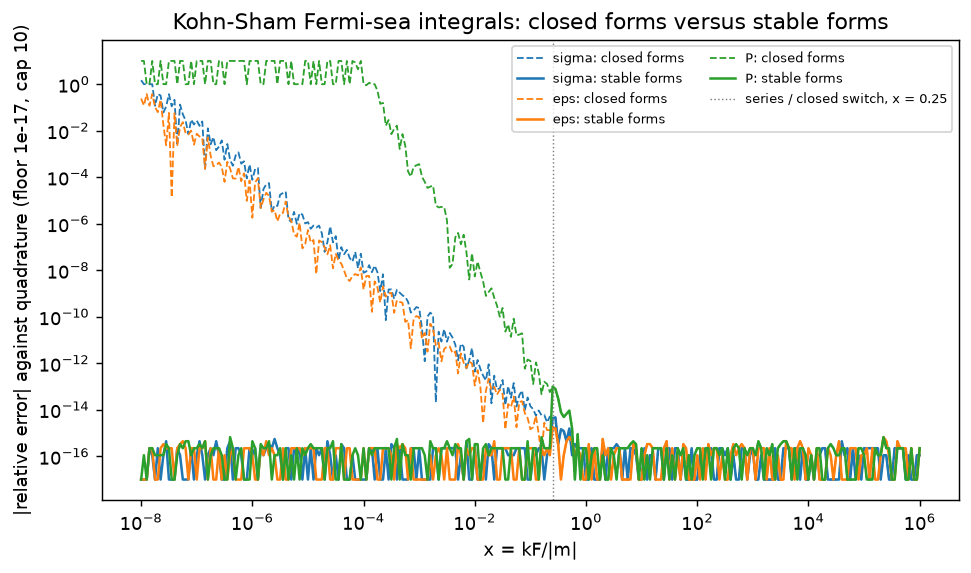
\includegraphics[width=0.9\linewidth]{nb05_ks_accuracy.png}
  \caption{\texttt{fable-cosmology/\allowbreak results/\allowbreak nb05\_ks\_accuracy.png} (notebook 05, section 5.1): the accuracy of
  the stable forms of the Fermi-sea integrals against adaptive quadrature, and of the closed forms.}
  \label{fig:nb05ks}
\end{figure}
\begin{figure}[htbp]
  \centering
  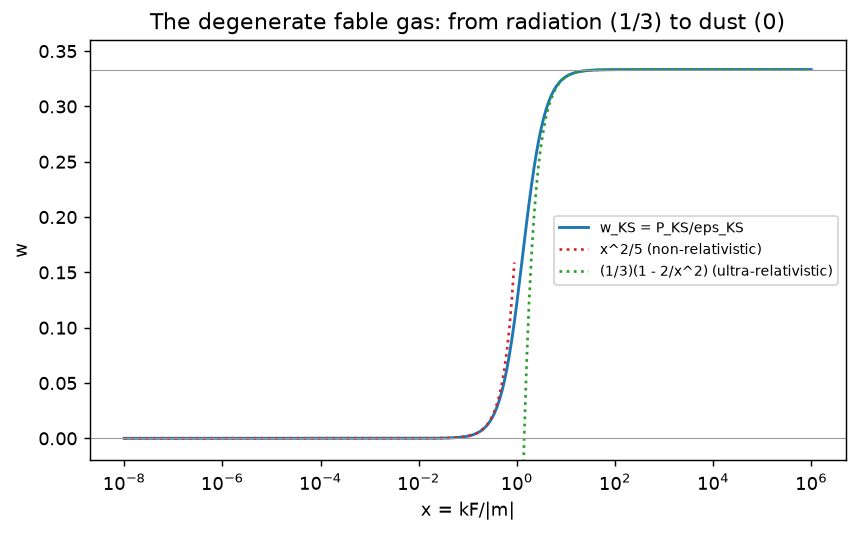
\includegraphics[width=0.75\linewidth]{nb05_w_ks.png}
  \caption{\texttt{fable-cosmology/\allowbreak results/\allowbreak nb05\_w\_ks.png} (notebook 05, section 5.2): $w_{\KS}(x)=\PKS/\epsKS$
  against $x=\kF/|m|$, from 0 (dust) to $1/3$ (radiation).}
  \label{fig:nb05wks}
\end{figure}

\subsubsection{The gap equation: uniqueness, branch selection, parameter domains}
\label{sec:4.5.3}

$f(m)=m-W'\bigl(\sigKS(m,\kF)/v\bigr)$. Since $\sigKS$ is odd and increasing in $m$ with slope
$\chi=d\sigKS/dm\leq\chi_0=g\kF^2/(4\pi^2)$, $f'=1-W''\chi/v$: the root is \textbf{unique} when $W''\leq0$
(attractive, concave $W$) or when $W''\chi_0/v<1$; otherwise there can be several roots [prose nb05 \S4;
file: \file{kohn_sham.rs}, module documentation]. Every potential states where its roots can lie and
whether the root is provably unique there (\cfcode{Potential::gap_plan} in \file{potentials.rs}). The
adopted parameter domains (design review DFT-16): \cfcode{expdamp} $m_0>0$, $s_1>0$ (the gap then pins
$0<\sigma<\min(n,s_1)$ strictly); \cfcode{power} $\lambda>0$, $0<\nu<1$, $\sigma$ in $(0,n)$ (the bare mass
$m_0$ may come out negative: \secref{sec:4.7.8}); \cfcode{quadratic} $\lambda<0$ unique, $\lambda>0$ all
roots enumerated.

\paragraph{Branch selection.} When several roots exist, the solver takes the one of \textbf{lowest}
energy density $\rho$ --- not the minimum of the Kohn--Sham energy $E_n[\sigma]$ over $\sigma$ in $(-n,n)$.
The no-sea functional is a minimax: its kinetic part $T_s=\epsKS(m(\sigma))-m(\sigma)\,\sigma$ is
\textbf{concave} ($d^2T_s/d\sigma^2=-1/\chi<0$), so the physical root is a \textbf{maximum} of $E_n$ over
$\sigma$, and its infimum is the variational collapse $E_n\to-|m_0|\,n$ as $\sigma\to-n$ (every particle
in the negative-mass band, i.e.\ in states of the Dirac sea). For attractive $W$ the auxiliary-field
\textbf{Walecka functional} $\Omega_n(m)=\epsKS(m)+W(\sigma_m)-m\,\sigma_m$, $W'(\sigma_m)=m$, is convex and
minimized at the gap root, with $\Omega_n(m^*)=\rho$. The numbers are in \secref{sec:4.6.1}.

\subsubsection{The energy--momentum tensor's expectation: \texorpdfstring{$\rho$, $P_{\mathrm{obs}}$, $P_{\mathrm{hid}}$}{rho, P\_obs, P\_hid}, and \texorpdfstring{$w$}{w}}
\label{sec:4.5.4}

On the gap:
\begin{align*}
  \rho&=3\PKS/v+W(\sigma_7) &&\text{(Section~29's trace identity $\varepsilon-3P=m\sigma$, per 7-volume)},\\
  \Pobs&=\PKS/v+\sigma_7W'-W,\\
  \Phid=\PC&=\sigma_7W'-W,\\
  \Pobs-\Phid&=\PKS/v\geq0 &&\text{(for every $W$: the Fermi gas can source}\\
  & &&\text{\phantom{(}$a_4''<0$, \secref{sec:4.2.6})},\\
  w_f&=\Pobs/\rho .
\end{align*}
The split $\rho=\rho_{\mathrm{qp}}+\rho_U$ with $\rho_{\mathrm{qp}}:=\epsKS/v$ (quasiparticles,
$w_{\mathrm{qp}}=\wDM=\PKS/\epsKS$ in $[0,1/3]$) and $\rho_U:=W-\sigma_7W'$ (the mean-field condensate,
with $P=-\rho_U$ along \textbf{all seven} spatial directions: an 8-dimensional vacuum energy that varies
with $\sigma$) is a \textbf{convention} [prose nb06 \S3; file: \file{kohn_sham.rs}].
\Secref{sec:4.5.10} defines the dark-matter and dark-energy equations of state built on it.

\subsubsection{Theorem: the Kohn--Sham fluid is exactly conserved in 8-dimensional Bianchi-I}
\label{sec:4.5.5}

The fable number in a comoving 7-volume, $(n_{\KS}/v)\,A^3v=n_{\KS}A^3$, is conserved, so $\kF=k_{F0}/A$.
Take $A$, $B$, $C$ and the mass $m(x_4)>0$ as \textbf{arbitrary} functions and $W$ arbitrary. Then,
identically,
\[
  \rho'+3H_A\,(\rho+\Pobs)+(3H_B+H_C)\,(\rho+\Phid)=\sigma_7\,\frac{d}{dx_4}\bigl[m-W'(\sigma_7)\bigr] .
\]
The right-hand side is the time derivative of the gap equation; on the self-consistent solution it
vanishes at every $x_4$, so the Kohn--Sham fluid obeys \secref{sec:4.3.5}'s conservation law (with
$\PC=\Phid$) \textbf{exactly}, for every $W$ --- the Einstein equations with this source are consistent.
The mechanism: $\rho+\Pobs=\wF\,n_{\KS}/v$ and $\rho+\Phid=\epsKS/v$ hold identically,
$d\varepsilon=\wF\,dn+\sigma\,dm$, and the gap cancels the $\sigma\,dm$ term against the variation of $W$.
Off the gap the fluid is \textbf{not} conserved. \cfproved{VIII \S33}
\begin{itemize}
  \item \cfL{CONSERVATION [definition]: the fable number per comoving 7-volume, (n\_KS/v) A\textasciicircum{}3 B\textasciicircum{}3 C, is constant when kF = kF0/A}
  \item \cfL{CONSERVATION [has content]: rho + P\_obs == wF n\_KS/v and rho + P\_hid == eps\_KS/v identically (no gap needed)}
  \item \cfL{CONSERVATION [THE RESULT]: rho' + 3 H\_A (rho + P\_obs) + (3 H\_B + H\_C)(rho + P\_hid) == sigma7 d/dx4[m - W'(sigma7)] IDENTICALLY, for arbitrary A, B, C, m(x4) > 0 and W: the KS fluid is exactly conserved on the gap}
  \item \cfL{CONSERVATION [control]: without the gap the fluid is NOT conserved -- the left side is not identically zero (witnessed on A = 1 + x4/2, B = 1 + x4/3, C = 1 + x4\textasciicircum{}2/3, m = 2 + x4, W = sigma\textasciicircum{}2, kF0 = 1, g = 8)}
\end{itemize}

The solver's form of the same law: $d\rho_8=\wF\,dn/v-(\varepsilon/v)\,d\ln v$, so at fixed $v$,
$d\rho_8/dn_8=\wF$ [file: \file{kohn_sham.rs}, module documentation]; its unit test
\file{kohn_sham::tests::thermodynamic_identities_at_the_self_consistent_point} and the end-to-end test
\file{covariant_conservation_along_real_fable8d_runs} check it [file: \file{kohn_sham.rs},
\file{tests/cosmology.rs}].

\subsubsection{The hidden-sheet driver}
\label{sec:4.5.6}

With $\PC=\Phid$, \secref{sec:4.3.4}'s evolution equations for $B$ and $C$ both read
\[
  H_B'+H_B\Theta=H_C'+H_C\Theta=\kappa F/6,\qquad F=\rho-3\Pobs+2\Phid .
\]
$F$ is the driver of the hidden sheet:
\begin{center}
\small
\renewcommand{\arraystretch}{1.3}
\begin{tabular}{@{}>{\raggedright\arraybackslash}p{0.52\linewidth}>{\raggedright\arraybackslash}p{0.42\linewidth}@{}}
\toprule
source & $F$\\
\midrule
radiation ($\Pobs=\rho/3$, $\Phid=0$) & $0$\\
dust & $\rho$\\
an 8-dimensional vacuum energy (all seven pressures $-\rho$; a bare $V_0$, the condensate $\rho_U$) & $2\rho$\\
the Kohn--Sham fable, on the gap & $2W-\sigma_7W'$ (off the gap: $\sigma_7(m-W')+2W-\sigma_7W'$)\\
the author's mass term $W=m_0\sigma$ & $m_0\sigma_7$ (like dust)\\
$W=V_0+m_0\sigma$ & $2V_0+m_0\sigma_7$\\
\bottomrule
\end{tabular}
\end{center}
\cfproved{VIII \S33}
\begin{itemize}
  \item \cfL{DRIVER [THE RESULT]: with P\_C = P\_hid, kappa (P\_hid - T/6) == kappa (P\_C - T/6) == kappa F/6, F = rho - 3 P\_obs + 2 P\_hid: the right-hand side of the B and C equations}
  \item \cfL{DRIVER [has content]: F == 0 for radiation, F == rho for dust, F == 2 rho for an 8D vacuum}
  \item \cfL{DRIVER [THE RESULT]: for the KS fluid F == sigma7 (m - W') + 2 W - sigma7 W' identically, i.e. F == 2 W - sigma7 W' on the gap; the mass term gives F == m0 sigma7 (dust-like), W = V0 + m0 sigma gives 2 V0 + m0 sigma7}
\end{itemize}

\subsubsection{Theorem: a frozen hidden sheet makes the fable radiation}
\label{sec:4.5.7}

Given $H_B=H_C=0$ at one time, the hidden sheet stays \textbf{frozen} for all time iff $F=0$ along the
history; for the Kohn--Sham fluid, for all $\sigma_7$ the history sweeps, iff $\sigma W'=2W$, i.e.
$W=c\,\sigma^2$. The gap is then $m=2c\,\sigma_7$, and $m=0$ is always a root. For $c<0$ it is the only one
($m\,\sigKS>0$ for $m\neq0$, so a root $m\neq0$ would give $m^2=2c\,(m\,\sigKS)/v<0$). For $c>0$ a
non-trivial root exists iff $c\,g\,\kF^2/(2\pi^2v)>1$ ($\sigKS/m$ decreases strictly, from $g\kF^2/(4\pi^2)$
at $m\to0$ to 0 at $m\to\infty$), and it has \textbf{higher} energy: on it
$\rho=\bigl(\epsKS(m)-m\,\sigKS(m)/2\bigr)/v$, and $\Delta(m)=\epsKS(m)-m\,\sigKS/2-\epsKS(0)$ vanishes at
$m=0^+$ with
\[
  \frac{d\Delta}{dm}=\frac{g\,m^3}{4\pi^2}\,\Bigl(\mathcal L-\frac{\kF}{\wF}\Bigr)>0
\]
($\mathcal L-\kF/\wF=\varphi(\kF/m)$, $\varphi(x)=\ln\bigl(x+\sqrt{1+x^2}\bigr)-x/\sqrt{1+x^2}$, which
vanishes at 0 and has derivative $x^2/(1+x^2)^{3/2}>0$). So the ground state of a frozen-compatible fable
is the $m=0$ branch, on which $\rho=\epsKS(\kF,0)/v$, $\Pobs=\rho/3$, $\Phid=0$: \textbf{radiation}. A
Kohn--Sham fable compatible with a frozen hidden sheet is neither dark matter nor dark energy.
\cfproved{VIII \S33}
\begin{itemize}
  \item \cfL{FROZEN [THE RESULT]: 2 W - sigma W' == 0 for all sigma iff W == c sigma\textasciicircum{}2 (the general solution of sigma W' == 2 W)}
  \item \cfL{FROZEN [has content]: m sigma\_KS > 0 for m > 0 (zero at kF = 0, kF-derivative g kF\textasciicircum{}2 m\textasciicircum{}2/(2 pi\textasciicircum{}2 wF) > 0; even in m, so also for m < 0); for c < 0 a root m != 0 of m = 2 c sigma\_KS/v would give m\textasciicircum{}2 = 2 c (m sigma\_KS)/v < 0: only m = 0}
  \item \cfL{FROZEN [has content]: phi(x) = Log[x + Sqrt[1 + x\textasciicircum{}2]] - x/Sqrt[1 + x\textasciicircum{}2] is 0 at x = 0 and increasing (derivative x\textasciicircum{}2/(1 + x\textasciicircum{}2)\textasciicircum{}(3/2)), hence positive for x > 0; and L - kF/wF == phi(kF/m)}
  \item \cfL{FROZEN [THE RESULT]: for c > 0, sigma\_KS/m decreases strictly (d/dm = -(g m/(2 pi\textasciicircum{}2))(L - kF/wF)) from g kF\textasciicircum{}2/(4 pi\textasciicircum{}2) at m -> 0 to 0 at m -> infinity: a non-trivial root of 1 = 2 c (sigma\_KS/m)/v exists iff c g kF\textasciicircum{}2/(2 pi\textasciicircum{}2 v) > 1}
  \item \cfL{FROZEN [THE RESULT]: on the non-trivial root (m = 2 c sigma7) rho == (eps\_KS - m sigma\_KS/2)/v, and Delta = eps\_KS(m) - m sigma\_KS/2 - eps\_KS(0) has Delta(0+) = 0 and dDelta/dm = (g m\textasciicircum{}3/(4 pi\textasciicircum{}2))(L - kF/wF) > 0: the m = 0 branch has LOWER rho}
  \item \cfL{FROZEN [has content]: witness numbers -- at g = 8, v = 1, c = 15, kF = 1 the non-trivial root m* exists (gap residual < 10\textasciicircum{}-20) and rho(m = 0) < rho(m*)}
  \item \cfL{FROZEN [THE RESULT]: on the m = 0 branch the frozen-compatible fable is RADIATION: rho = eps\_KS(kF, 0)/v, P\_obs = rho/3, P\_hid = 0}
\end{itemize}
The witness the run prints \cfdisplayed{VIII \S33}, \file{claude-fable/run_fermion_fable_part8.log}:
\begin{Verbatim}[fontsize=\scriptsize]
  frozen-compatible witness (g = 8, v = 1, c = 15, kF = 1): non-trivial root m* = 3.97853200077825223420767254928521681893`12.;  rho(m = 0) = 0.10132118364233777144387946320972763891`12.  <  rho(m*) = 0.28374208489508058306307225309709278221`12.
\end{Verbatim}

\subsubsection{The classical limit, and the sign rule}
\label{sec:4.5.8}

The classical limit is the \textbf{non-relativistic} limit $\kF\ll|m|$ (not a coherent zero mode: the
Pauli principle forbids that). Exactly, on the gap, with $s=H\sigma_7$ and $V(s):=W(s/H)$:
\[
  \rho=V(s)+3\PKS/v,\qquad \Pobs=s\,V'(s)-V(s)+\PKS/v,\qquad \Phid=s\,V'(s)-V(s),
\]
and as $\kF/m\to0$ ($m>0$), $\sigKS/n_{\KS}=1-\tfrac{3}{10}\,\kF^2/m^2+\dots$,
$(\epsKS-n_{\KS}m)/(n_{\KS}\kF^2/m)\to3/10$, $\PKS/(n_{\KS}\kF^2/m)\to1/5$: $\PKS/\rho\to0$ and the quantized
fluid reduces to Part~VI's $\rho=V(s)$, $P=s\,V'(s)-V(s)$ (its $K_h=0$ branch); $\Phid$ is exactly Part~VI's
on-shell pressure. With $s_0=n_{\KS}/v$, exactly on the gap,
\[
  \rho-W(s_0)=(\varepsilon-n\,m)/v-\bigl[W(s_0)-W(\sigma_7)-W'(\sigma_7)\,(s_0-\sigma_7)\bigr]:
\]
a second-order Taylor remainder in $s_0-\sigma_7$. \textbf{The sign rule:} $m\,\sigKS\geq0$, so on every
self-consistent solution $\operatorname{sign}(\sigma_7)=\operatorname{sign}(m)=\operatorname{sign}\bigl(W'(\sigma_7)\bigr)$;
for Part~VI's mass term $W=-2M\sigma$ the gap is $m=-2M$ and $\rho\to2|M|\,n/v>0$ --- the Part~VI branch
$Ms>0$, of negative energy, is not a self-consistent state. \cfproved{VIII \S33}
\begin{itemize}
  \item \cfL{CLASSICAL LIMIT [THE RESULT]: exactly, on the gap and with s = H sigma7, V(s) = W(s/H): rho == V(s) + 3 P\_KS/v, P\_obs == s V'(s) - V(s) + P\_KS/v, P\_hid == s V'(s) - V(s)}
  \item \cfL{CLASSICAL LIMIT [fidelity]: Section 24's on-shell P\_1 (cfP1Fable, re-checked here) is s V'(s) - V(s); evaluated at s = H sigma7 with V(s) = W(s/H) it IS the KS P\_hid = sigma7 W' - W}
  \item \cfL{CLASSICAL LIMIT [THE RESULT]: NR series (kF/m -> 0, m > 0): sigma\_KS/n\_KS = 1 - (3/10) kF\textasciicircum{}2/m\textasciicircum{}2 + ..., (eps\_KS - n\_KS m)/(n\_KS kF\textasciicircum{}2/m) -> 3/10, P\_KS/(n\_KS kF\textasciicircum{}2/m) -> 1/5}
  \item \cfL{CLASSICAL LIMIT [has content]: the design's form, exactly: on the gap (m = W'(sigma7) > 0) rho - W(s0) == (eps - n m)/v - [W(s0) - W(sigma7) - W'(sigma7)(s0 - sigma7)], s0 = n/v -- a second-order Taylor remainder in s0 - sigma7}
  \item \cfL{SIGN RULE [THE RESULT]: m sigma\_KS >= 0 gives sign(sigma7) == sign(m) == sign(W'(sigma7)); for Section 24's mass term W = -2 M sigma the gap is m = -2 M and W(sign(m) n/v) = -2 M sign(-2 M) n/v == 2 |M| n/v > 0}
\end{itemize}
Notebook 05 checks the series at $x=0.001$ and the sign at $m=-2$ \cfnb{nb05 \S5.4}:
\cfcode{(sigma/n - 1)/x^2 = -0.300000 (-3/10)}, \cfcode{(eps/(|m| n) - 1)/x^2 = +0.300000 (+3/10)},
\cfcode{P/(n kF^2/|m|) = 0.200000 (1/5)}; \cfcode{m = -2: sigma/n = -0.999999700: sgn(sigma) = sgn(m)}.

\subsubsection{\texorpdfstring{$w_f\geq-1$}{w\_f >= -1}: no phantom crossing}
\label{sec:4.5.9}

\[
  \rho+\Pobs=\wF\,n_{\KS}/v\geq0\qquad\text{so}\qquad w_f\geq-1\ \text{ wherever } \rho>0 .
\]
The quantized fermion fable \textbf{cannot cross the phantom divide}; the classical crossing of Part~VI
(\secref{sec:3.1.12.7}, at $V'(s^*)=0$) does not survive quantization. \cfproved{VIII \S33}
\cfL{PHANTOM [THE RESULT]: rho + P\_obs == wF n\_KS/v >= 0, so w\_f >= -1 wherever rho > 0 -- the quantized fable cannot cross the phantom divide}. Notebook 05 compared the classical $w_{\mathrm{cl}}=s\,V'/V-1$ of five of
Part~VI's potential shapes with the quantum $w=\Pobs/\rho$ of the lowest-energy gap root, over densities
$10^{-3}\leq n\leq30$ (in units where the classical $s$ equals $n$), for $W=\mathcal A\,V$ with
$\mathcal A=10^4,10^2,1$ --- a large $\mathcal A$ makes the quasiparticles heavy ($m=\mathcal A\,V'$), which
is the classical limit (915 points) \cfnb{nb05 \S5.4, file:
\file{fable-cosmology/results/nb05_classical_vs_quantum.csv}, figure \file{nb05_classical_vs_quantum.png}}
(figure~\ref{fig:nb05cq}):
\begin{center}
\small
\renewcommand{\arraystretch}{1.3}
\begin{tabular}{@{}>{\raggedright\arraybackslash}p{0.36\linewidth}>{\raggedright\arraybackslash}p{0.3\linewidth}>{\raggedright\arraybackslash}p{0.28\linewidth}@{}}
\toprule
potential ($V(s)$) & classical $\min w_{\mathrm{cl}}$ & quantum $\min w$ ($\mathcal A=10^4$, $100$, $1$)\\
\midrule
mass ($s$) & \texttt{+0.0000}, never crosses $-1$ & \texttt{+0.00000}, \texttt{+0.00000}, \texttt{+0.00741}\\
lambda-mass ($0.7+0.3\,s$) & \texttt{-0.9996}, never crosses $-1$ & \texttt{-0.99957}, \texttt{-0.99957}, \texttt{-0.99949}\\
power ($s+s^{0.236}$) & \texttt{-0.7601}, never crosses $-1$ & \texttt{-0.76012}, \texttt{-0.76012}, \texttt{-0.76012}\\
expdamp ($1.566+0.839\,s\,e^{-s/2.21}$) & \texttt{-1.3020}, \textbf{crosses $-1$} at $n=2.2047$ & \texttt{-0.99952}, \texttt{-0.99947}, \texttt{-0.99945}\\
lorentz ($1+s/(1+(s/1.5)^2)$) & \texttt{-1.2481}, \textbf{crosses $-1$} at $n=1.4999$ & \texttt{-0.99900}, \texttt{-0.99900}, \texttt{-0.99898}\\
\bottomrule
\end{tabular}
\end{center}
and it printed \cfcode{the quantum w >= -1 at every density, every A and every potential; the classical expdamp and lorentz cross -1}.
For \cfcode{expdamp} the gap keeps $0<\sigma<\min(n,s_1)$ strictly, with $\sigma\to s_1$ and $m\to0$ only as
$n\to\infty$ (solver test
\file{kohn_sham::tests::expdamp_pins_sigma_below_s1_and_mass_goes_to_zero_at_high_density}).

\begin{figure}[htbp]
  \centering
  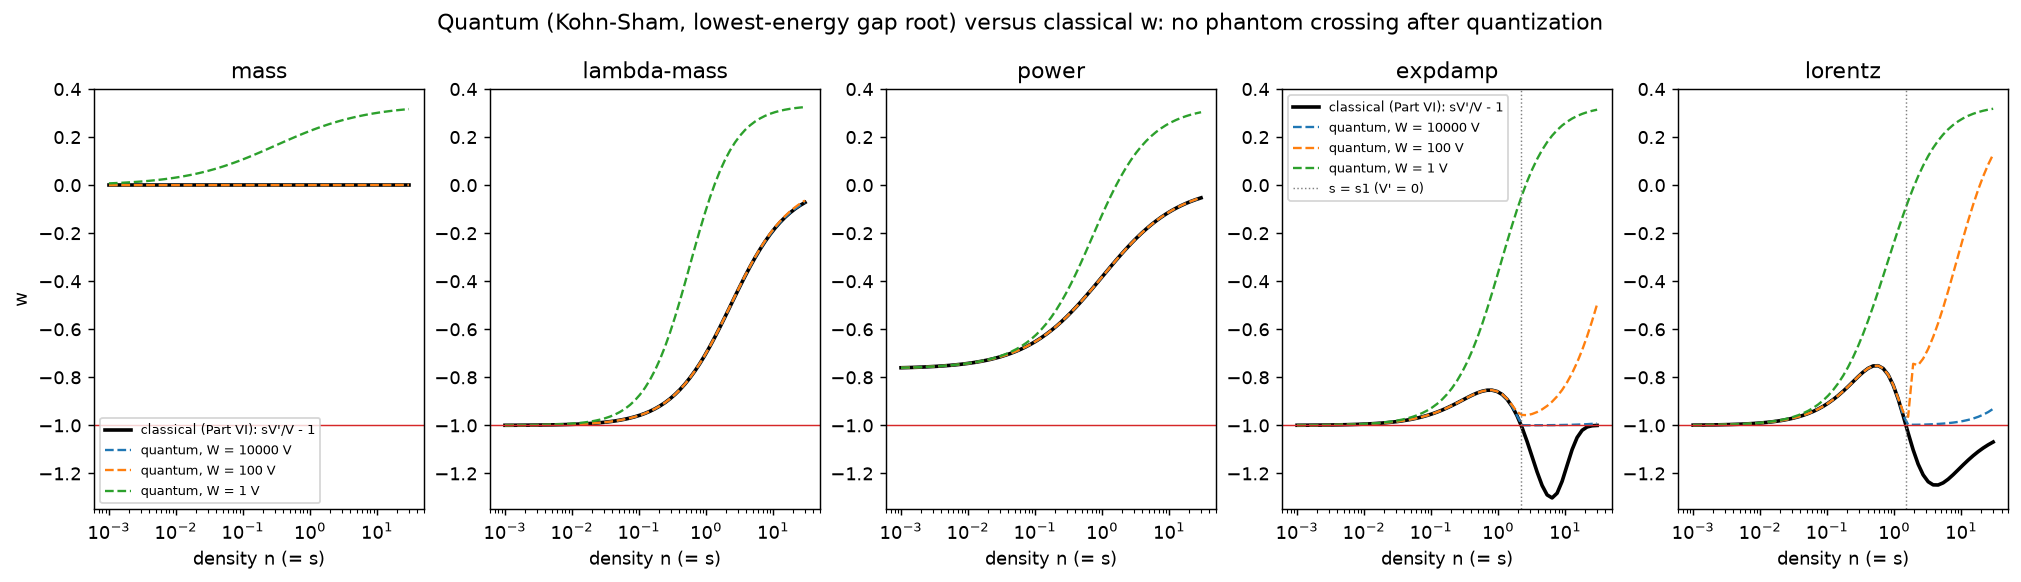
\includegraphics[width=0.95\linewidth]{nb05_classical_vs_quantum.png}
  \caption{\texttt{fable-cosmology/\allowbreak results/\allowbreak nb05\_classical\_vs\_quantum.png} (notebook 05, section 5.4): the
  classical $w_{\mathrm{cl}}=s\,V'/V-1$ against the quantum $w=\Pobs/\rho$ of the lowest-energy gap root.}
  \label{fig:nb05cq}
\end{figure}

\subsubsection{The equations of state an observer can define}
\label{sec:4.5.10}

Four definitions are used, and they must not be confused [file: \file{models.rs}, documentation of the
output columns; prose nb06 \S5]:
\begin{enumerate}
  \item $\boldsymbol{w_f=P_{\mathrm{obs},f}/\rho_f}$ --- the intrinsic equation of state of the whole fable
        fluid;
  \item $\boldsymbol{\wDM=w_{\mathrm{qp}}=\PKS/\epsKS}$ --- the intrinsic equation of state of the
        quasiparticles, in $[0,1/3]$;
  \item $\boldsymbol{\wDMeff=\wDM-\sigKS\,(dm/dN)/(3\epsKS)}$ --- the effective equation of state of the
        quasiparticles when the mass varies, which exchange energy with the condensate at the rate
        $Q=\sigma_8\,dm/dt$ (the exact exchange; $n\,dm/dt$ is its non-relativistic limit);
  \item $\boldsymbol{\wDE}$ --- the dark energy an observer \textbf{infers} by fitting cold dark matter plus
        dark energy: $\rhoDE=H_A^2-\Omega_{r0}A^{-4}-\Omega_{b0}A^{-3}-\mtoday\,n_{\mathrm{today}}A^{-3}$
        (radiation, baryons, and cold dark matter with \textbf{today's} mass $\meffx(A=1)$ subtracted),
        $\wDE=-1-\tfrac13\,d\ln\rhoDE/d\ln A$.
\end{enumerate}
The adiabatic sound speed of the fable is $c_s^2=(dP_{\mathrm{obs},f}/dN)/(d\rho_f/dN)$; $c_s^2<0$ is an
adiabatic instability. The split into dark matter and dark energy is a convention (\secref{sec:4.5.4}): the
condensate is an 8-dimensional vacuum energy.

\subsubsection{The vacuum energy of mass-varying potentials}
\label{sec:4.5.11}

For a constant mass the Dirac-sea energy is a constant; it is absorbed into $V$ and appears as a bare
cosmological constant. \textbf{The cosmological-constant problem is not solved here.} For a mass that
varies along the history the sea energy cannot be absorbed silently (design review DFT-4, adopted). The
renormalized one-loop Dirac-sea energy that the no-sea functional drops (relativistic Hartree
approximation, Chin 1977), per 3-volume, with reference mass $M$ and counterterms through $m^4$, is
\[
  \Evac(m)=-\frac{g}{16\pi^2}\Bigl[m^4\ln\frac mM+M^3(M-m)-\frac72M^2(M-m)^2+\frac{13}{3}M(M-m)^3-\frac{25}{12}(M-m)^4\Bigr]
\]
[file: \file{kohn_sham.rs}, function \cfcode{vacuum_energy}; its test
\file{kohn_sham::tests::vacuum_energy_vanishes_to_fifth_order_at_the_reference_mass}]. At $m=0$ the
bracket is $M^4\bigl(1-\tfrac72+\tfrac{13}{3}-\tfrac{25}{12}\bigr)=-M^4/4$, so
$\Evac(0)-\Evac(M)=g\,M^4/(64\pi^2)$ \cfderived. With $g=8$ and $\Ec=\rhoc^{1/4}=2.46261\times10^{-3}$\,eV
(asserted: \cfL{fable4d RUNS [definition]: the units computed from CODATA 2018 -- E\_c = rho\_c0\textasciicircum{}(1/4) == 2.46261e-3 eV, Omega\_r0 == 9.2096e-5, Omega\_b0 = 0.02237/h\textasciicircum{}2 == 0.049243 (to the quoted digits)}), a mass variation of order $m$ changes the vacuum energy by
\begin{gather*}
  \frac{g\,m^4/(64\pi^2)}{\rhoc}=3.44,\quad 3.44\times10^{4},\quad 3.44\times10^{8},\quad 3.44\times10^{12}\\
  \text{at } m=0.01,\ 0.1,\ 1,\ 10\ \text{eV}\qquad\text{(it scales as $m^4$)}
\end{gather*}
[derived here: $g/(64\pi^2)=0.012665$, $(m/\Ec)^4=271.9$ at $m=0.01$\,eV]. So for $m\gtrsim10$\,meV it
exceeds the critical density; notebook 05 prints the exact threshold \cfnb{nb05 \S5.8}:
\cfcode{Delta E_vac(0; M) = g M^4/(64 pi^2): check 1.000000000000003;  g M^4/(64 pi^2) exceeds rho_c0 for M > (64 pi^2/g)^(1/4) E_c = 7.341 meV},
and at $M=1$\,eV it gives $|\Evac|/\rhoc$ $=$ \texttt{2.760e-02}, \texttt{2.802e+03}, \texttt{9.454e+06},
\texttt{3.444e+08} at $m/M=0.99$, $0.9$, $0.5$, $0$ (the last is the $3.44\times10^{8}$ above); at
$M=1000$\,eV, \texttt{3.444e+20} at $m=0$; the fifth-order zero at $m=M$ is confirmed by the ratio
\texttt{31.9470} ($2^5=32$).

The design review's refinement (DFT-4, adopted): the sea energy \textbf{can} be absorbed formally by
reading $W$ as the fully renormalized effective potential, $\Omega(m)=\epsKS+\Evac+F$ $=$ no-sea with
$\tilde F=F+\Evac$; that reading is a \textbf{fine-tuning} of the bare potential against the sea energy.
The vacuum also adds $\sigma_{\mathrm{vac}}=d\Evac/dm$ to $\langle\bar\Psi\Psi\rangle$. The two options are
(a) to include $\Evac$ in $\rho$ and in the gap equation, or (b) to declare $W$ the renormalized
potential. \textbf{The runs use (b)}, and they print $\Evac(m(t))-\Evac(\mtoday)$ in units of $\rhoc$ (the
solver's column \cfcode{vac_over_rhoc}, $\Evac\bigl(\meffx;M=\meffx(A=1)\bigr)/v$). Along the power run
$\nu=0.236$, $\mtoday=30$\,eV notebook 05 found \cfnb{nb05 \S5.8} (figure~\ref{fig:nb05vac}):
\begin{Verbatim}[fontsize=\scriptsize]
power nu = 0.236, m_today = 30 eV: m_eff/m_today runs from 0.2007 (a = 1e-12) to 1;  max |solver vac_over_rhoc - formula| / (g M^4/(64 pi^2)) = 5.4e-15
   |Delta E_vac(m(t)) - Delta E_vac(m_today)| / rho_total: max over a >= 0.3 = 1.314e+13,  at a = 0.5: 1.149e+13
\end{Verbatim}
\Secref{sec:4.7.6} gives the ratio for every run.

\begin{figure}[htbp]
  \centering
  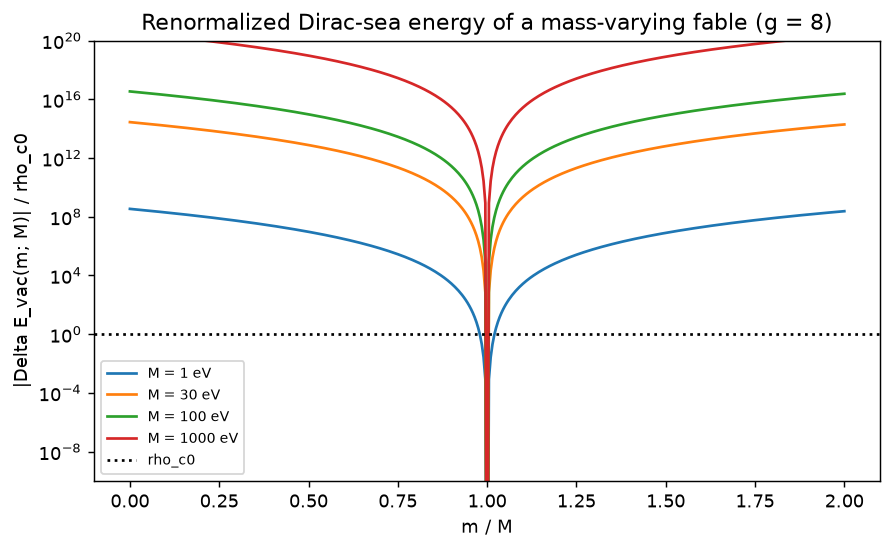
\includegraphics[width=0.9\linewidth]{nb05_vacuum_energy.png}
  \caption{\texttt{fable-cosmology/\allowbreak results/\allowbreak nb05\_vacuum\_energy.png} (notebook 05, section 5.8): the
  renormalized Dirac-sea energy of a mass-varying fable.}
  \label{fig:nb05vac}
\end{figure}

\subsubsection{Exchange and correlation}
\label{sec:4.5.12}

The Kohn--Sham functional of \secref{sec:4.6.1} has $E_{\mathrm{xc}}$ neglected (the Hartree mean field). For
the author's mass term ($W$ linear) the action is bilinear, the theory is free, and the mean field is
\textbf{exact} ($E_{\mathrm{xc}}=0$). For a nonlinear $W$ the design review (DFT-14) estimated that the Fock
exchange of the contact interaction is suppressed relative to the Hartree term by $\sim1/g=1/8$ only in
the non-relativistic regime $\kF\ll m$, and is of order one or larger for $\kF\gtrsim m$; in the
relativistic era its neglect is controlled only by the smallness of the interaction energy relative to
$3\PKS$. That ratio was not computed in the runs; the neglect of $E_{\mathrm{xc}}$ is a stated
approximation of every mass-varying result in this document.

% ===============================================================================================
\subsection{Density-functional theory: the fable ground and first excited states}
\label{sec:4.6}

The author asked to ``use some of the relevant ideas from Density Functional Theory to obtain the fable
ground and first excited states''. Two systems are treated: the \textbf{homogeneous} fable gas of the
present universe (sections~\ref{sec:4.6.1}--\ref{sec:4.6.2}), and the fable \textbf{along the hidden
coordinate $x_0$} of the primordial field, where the wall $x_0=0$ binds discrete states
(sections~\ref{sec:4.6.3}--\ref{sec:4.6.7}). The homogeneous numbers are printed by notebook 05
\cfnb{nb05 \S5.5, \S5.6}; the wall-state numbers are quoted from
\file{fable-cosmology/fermion/waveguide_REPORT.txt} \cfnb{WG n} and its logs, and notebook
\file{07_fable_dft_states.ipynb}, executed and committed in \texttt{aca5102}, reproduces them (a number it
prints again carries the mark \cfnb{nb07 \S n}, with the notebook's section). The development logs that the report names are files under
\file{fable-cosmology/fermion/dev/}, a folder the repository ignores; the report, which is tracked, quotes
them.

\subsubsection{The functional, and the homogeneous Kohn--Sham ground state}
\label{sec:4.6.1}

\paragraph{The functional.} For the conserved charge $n$ and the scalar density $\sigma$ (the
relativistic Hohenberg--Kohn--Sham scheme; the Serot--Walecka mean field is its Hartree limit), the
energy of the gas at fixed $n$ is
\begin{gather*}
  E_n[\sigma]=T_s(\sigma;n)+W(\sigma)+E_{\mathrm{xc}},\qquad T_s=\epsKS\bigl(m(\sigma)\bigr)-m(\sigma)\,\sigma,\qquad
  \sigKS\bigl(m(\sigma),\kF\bigr)=\sigma,\\
  \frac{dE_n}{d\sigma}=W'(\sigma)-m(\sigma)\quad\text{(stationary exactly at the gap roots)},\qquad
  \frac{d^2T_s}{d\sigma^2}=-\frac1\chi<0,
\end{gather*}
with $E_{\mathrm{xc}}$ neglected (\secref{sec:4.5.12}) and the Dirac sea excluded (the no-sea functional; its
energy is \secref{sec:4.5.11}). The Kohn--Sham Slater determinant is the filled Dirac sea (renormalized
away) plus the Fermi sea $|k|<\kF$ of the lowest positive band. \textbf{The ground state is the stationary
point of this minimax functional} --- a maximum in $\sigma$ and a minimum in the occupations --- and
\textbf{never} its minimum over $\sigma$ [prose nb05 \S5.6; solver: design departure D1 of the
development report, and the unit tests
\file{kohn_sham::tests::ks_functional_stationary_point_is_a_maximum_for_the_mass_term},
\file{walecka_functional_is_minimized_at_the_gap_root},
\file{multiple_gap_roots_are_found_and_the_lowest_energy_one_is_taken} in \file{kohn_sham.rs}]. For
linear $W$ the theory is free, $m=m_0$ exactly, and the Kohn--Sham state is the exact ground state.

\paragraph{The minimax, in numbers} \cfnb{nb05 \S5.6, file: \file{fable-cosmology/results/nb05_minimax.csv},
figure \file{nb05_minimax.png}} (figure~\ref{fig:nb05minimax}):
\begin{Verbatim}[fontsize=\scriptsize]
mass term W = 2 sigma, kF = 1.5: n = 0.4559453264, the gap root sigma* = 0.3961298703 (sigma*/n = 0.868810)
E_n(sigma*) = 1.052962422118 = rho = eps_KS(m0) = 1.052962422118;  max of E_n over the grid = 1.052959281278
E_n/n at sigma = -(1 - 1e-7) n: -1.999480  (the collapse value -|m0| = -2.0)

attractive W = sigma - 10 sigma^2, kF = 1: unique gap root m* = 0.2112489356, rho = 0.1211932853;  Omega_n(m*) = 0.121193285306
Omega_n on the grid: minimum 0.121193451922 at m = 0.2100;  second differences all positive (convex): True
\end{Verbatim}
The root of the mass term is the \textbf{maximum} of $E_n$ (the grid maximum lies just below it), and
$E_n/n$ falls to the collapse value $-|m_0|$ as $\sigma\to-n$. For the attractive $W$ the convex Walecka
functional $\Omega_n(m)=\epsKS(m)+W(\sigma_m)-m\,\sigma_m$ has its minimum at the gap root, equal to $\rho$.

\paragraph{Several roots, and a first-order transition.} For the repulsive
$W=m_0\sigma+(\lambda/2)\,\sigma^2$ with $(m_0,\lambda)=(0.05,20)$ at $\kF=1$,
$W''\chi_0=\lambda\,g\,\kF^2/(4\pi^2)=4.0528>1$ and there are three roots; the Rust solver's \cfcode{gap}
command and the Python solver agree \cfnb{nb05 \S5.5}:
\begin{Verbatim}[fontsize=\scriptsize]
# potential Quadratic { v0: 0.0, m0: 0.05, lam: 20.0 }, kF = 1e0, v = 1e0, n8 = 1.3509491152311703e-1, plan = Scan { lo: -2.651898230462341, hi: 2.7518982304623405 }
m,sigma8,rho8,P_obs,P_hid,gap_residual
-2.535353916022531e0,-1.292676958011266e-1,1.909782056219713e-1,1.772147779888931e-1,1.671013717773260e-1,8.506e-17
-1.640336879334347e-2,-3.320168439667173e-3,1.012381942988485e-1,3.387489103006236e-2,1.102351846776195e-4,-1.898e-17
2.644093986040535e0,1.297046993020268e-1,2.039272771420881e-1,1.779694075325236e-1,1.682330902102918e-1,0.000e0
# selected (Lowest): m = -1.640336879334347e-2, rho8 = 1.012381942988485e-1, roots = 3
\end{Verbatim}
with $(\rho+P)/(\wF n)=$ \texttt{1.000000000000} on every root (so $w\geq-1$ on every branch), and
\cfcode{uniqueness criterion lam chi0 < 1 holds for kF < 0.4967; three roots first appear at kF = 0.625 on this grid; the ground state jumps from m = +0.4756 (kF = 0.600) to m = -0.0998 (kF = 0.625)}
\cfnb{nb05 \S5.5, figure \file{nb05_gap_roots.png}} (figure~\ref{fig:nb05gap}): the ground state jumps
between branches --- a first-order transition. That is why the solver refuses a repulsive quadratic run
(\secref{sec:4.7.11}): energy conservation across the jump would need a Maxwell construction, which it does
not implement.

\begin{figure}[htbp]
  \centering
  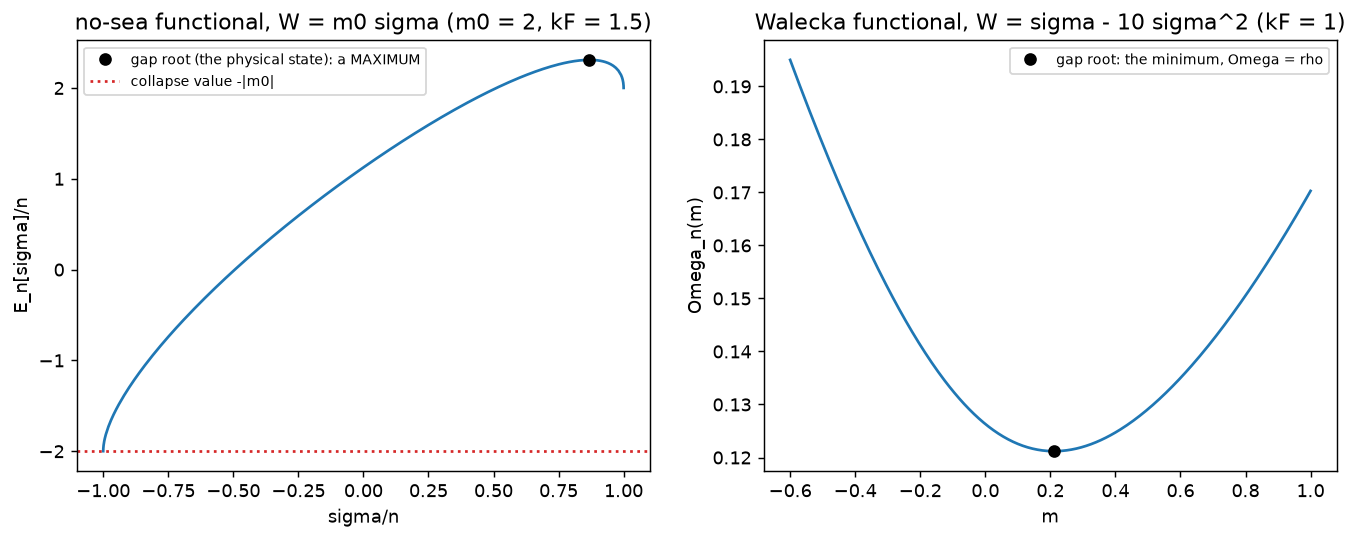
\includegraphics[width=0.95\linewidth]{nb05_minimax.png}
  \caption{\texttt{fable-cosmology/\allowbreak results/\allowbreak nb05\_minimax.png} (notebook 05, section 5.6): the no-sea
  Kohn--Sham functional $E_n[\sigma]$ of the mass term (its gap root is a maximum) and the Walecka
  functional $\Omega_n(m)$ of an attractive $W$ (its gap root is a minimum).}
  \label{fig:nb05minimax}
\end{figure}
\begin{figure}[htbp]
  \centering
  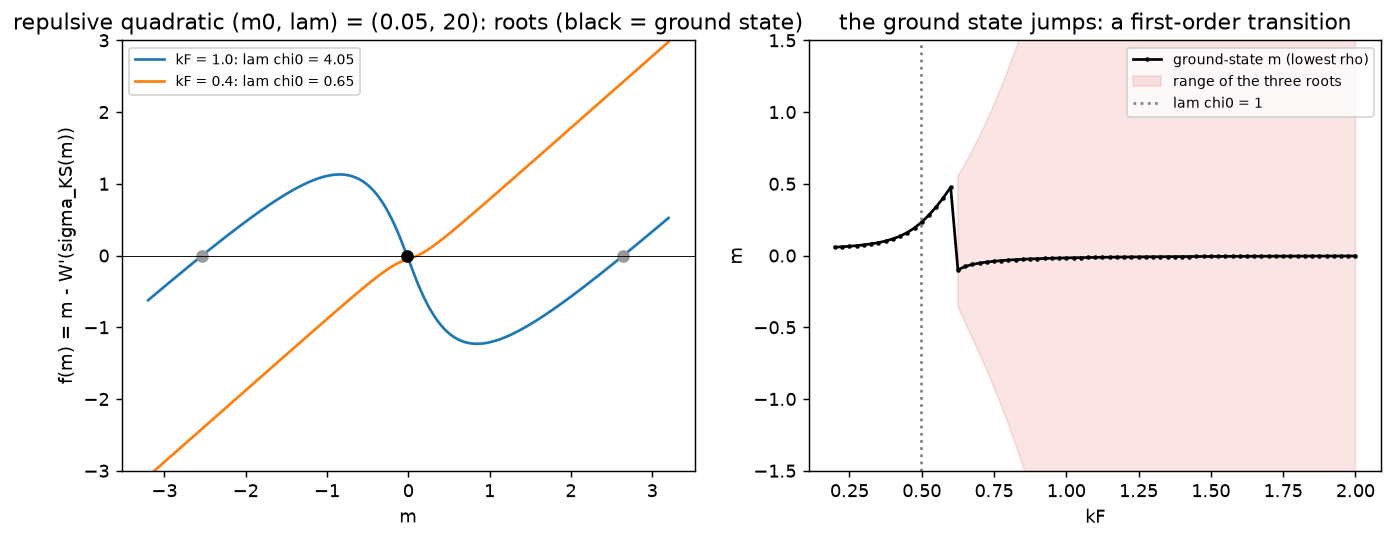
\includegraphics[width=0.95\linewidth]{nb05_gap_roots.png}
  \caption{\texttt{fable-cosmology/\allowbreak results/\allowbreak nb05\_gap\_roots.png} (notebook 05, section 5.5): the roots of the
  gap equation of the repulsive quadratic $W$ against $\kF$, and the jump of the ground state between
  branches.}
  \label{fig:nb05gap}
\end{figure}

\subsubsection{The first excited states of the homogeneous gas}
\label{sec:4.6.2}

The design review (DFT-15, adopted) states them; they are not assertions of the notebook, and the
derivation is short \cfderived:
\begin{itemize}
  \item \textbf{Particle--hole excitations} (a quasiparticle moved from just inside to just outside the
        Fermi surface) are \textbf{gapless}: $\Delta E\to0$ as the momentum transfer goes to zero. The
        lowest excited state of the gas is degenerate with the ground state in the thermodynamic limit,
        and it has no effect on $w$.
  \item \textbf{Pair excitations} create a particle above the Fermi sea (energy $\geq\wF$, momentum
        $|k_1|\geq\kF$) and a hole in the Dirac sea, an antiparticle (energy $\sqrt{k_2^2+m^2}\geq|m|$), with
        total momentum $q=k_1+k_2$. At $q=0$, $k_2=-k_1$, and the threshold is $2\wF$ (Pauli blocking
        pushes it from $2|m|$ to $2\wF$). The absolute threshold is $\wF+|m|$, at $|q|=\kF$ ($|k_1|=\kF$,
        $k_2=0$).
  \item \textbf{Delta-SCF} (moving one quantum and re-solving the gap): in the homogeneous gas one quantum
        changes $\sigma$ by $O(1/\text{volume})$, so the self-consistent excitation energy of one quantum
        equals the single-particle one. A finite effect needs a finite fraction of the particles, which is
        how the wall problem below defines its first excited state (design review DFT-9).
\end{itemize}

\subsubsection[{The states along the hidden coordinate: the problem [WG 2]}]{The states along the hidden coordinate: the problem \cfnb{WG 2}}
\label{sec:4.6.3}

The wall-state solver works at fixed observer's time on the canonical frame, with $a_4$ frozen to a
constant (the adiabatic approximation). The spectrum depends on the transverse momentum $k$ and the frozen
$a_4$ only through $K_\infty=k\,e^{a_4}$, so every number below is a function of $K_\infty$; the code works
with $K_\infty$ directly (internally it sets the frozen constant to zero, which only identifies $k$ with
$K_\infty$; nothing here or in the notebook gives $a_4$ a value). Units: $H=1$, $\hbar=c=1$. Its
derivation, \file{fable-cosmology/fermion/waveguide_derivation.wls}, loads the notebook's own Input cells
1--117 (with \cfcode{DumpSave} blocked) and uses only the notebook's objects (\cfcode{T16},
\cfcode{sigma16}, \cfcode{gammaCurvedCanonical}, \cfcode{GammaSpinCanonical}, \cfcode{cfDcov16},
\cfcode{gCanonical}, \cfcode{RicciScalarCanonical}, \cfcode{eta4488}); its log records
\cfcode{94 checks, 94 PASS, 0 FAIL} in 162.8\,s (\cfcode{total time 162.8 s}, with cells 1--117
evaluated in \cfcode{125. s}, in the run of 2026-09-25 00:06:38 that wrote the committed
\file{waveguide_T16.json}; the first committed run, in \texttt{18a2501}, took 171.4\,s, with 132.3\,s of
loading), and that the notebook's own 142 assertions of cells
1--117 passed while loading [file: \file{fable-cosmology/fermion/waveguide_derivation.log}].

\paragraph{The reduction.} With $\Psi=e^{ikx_1-i\omega x_4}\sqrt{\sin 6Hx_0}\;\Psi'(x_0)$ the Dirac equation
$\gamma^\mu D_\mu\Psi=m\Psi$ ($m=H\,V'(s)$; $m=-2M$ for the author's mass term) becomes \textbf{exactly}
\begin{gather*}
  (\gamma^\mu D_\mu-m)\,\Psi=\sqrt{\sin}\;e^{(\dots)}\Bigl[\cot\,T_0\,\partial_0+i\,k\,e^{A_4}\sin^{1/6}\,T_1-i\,\omega\,T_4-m\Bigr]\Psi',\\
  T_0\,\partial_z\Psi'+i\,K(z)\,T_1\Psi'-i\,\omega\,T_4\Psi'=m\,\Psi',\qquad
  K(z)=K_\infty\bigl(1-e^{-12Hz}\bigr)^{1/12},\qquad K_\infty=k\,e^{a_4}
\end{gather*}
in the proper distance $z=-\ln\cos(6Hx_0)/(6H)$ ($\cot\,d/dx_0=d/dz$; $z=0$ at the wall, a finite proper
distance away; $z\to\infty$ as $6Hx_0\to\pi/2$). The measure is
$\sqrt{|g|}\,|\Psi|^2dx_0=|\Psi'|^2dz$, so the one-particle space is $L^2(dz)$. The transverse term rises
from $K(0)=0$ at the wall ($K=K_\infty(12Hz)^{1/12}(1-Hz/2+\dots)$, $K'$ integrable) to $K_\infty$: a
``pocket'' of width $\sim1/(12H)$ ($K^2/K_\infty^2=0.875776$, $0.942018$, $0.984275$ at $z=0.05$, $0.1$,
$0.2/H$). The wall is a curvature singularity at finite proper distance: $R\,z^2\to-31/24$ as $z\to0$.

\paragraph{Hamiltonian form and the $2\times2$ blocks.} $\omega\,\phi=h\,\phi$,
$h=-i\,\alpha_z\,\partial_z+K(z)\,\alpha_x+m\,\beta$ with $\alpha_z=-T_4T_0$, $\alpha_x=-T_4T_1$,
$\beta=-i\,T_4$ (Hermitian involutions, pairwise anticommuting); $J=-i\,T_0T_1T_2T_3T_4$ commutes with $h$.
$w_3=\alpha_z\alpha_x\beta$ ($w_3^2=-1$) is central; the algebra $\langle\alpha_z,\alpha_x,\beta,J\rangle$ has
dimension 16, and $\mathbb C^{16}$ splits into \textbf{8 invariant 2-dimensional blocks}: 4 with $w_3=-i$
($J=+1$ twice, $J=-1$ twice) and 4 with $w_3=+i$. In an explicit block basis every block has
$\alpha_z=\sigma_y$, $\beta=\sigma_z$, $T_0=\sigma_x$, and with $\phi=(f,g)$:
\begin{align*}
  \text{irrep } w_3=-i:&\qquad f'=-K(z)\,f+(m+\omega)\,g,\qquad g'=K(z)\,g+(m-\omega)\,f,\\
  \text{irrep } w_3=+i:&\qquad \text{the same with } K\to-K .
\end{align*}

\paragraph{The wall conditions.} The self-adjoint conditions of a block are exactly the real lines
$f(0)\cos\vartheta+g(0)\sin\vartheta=0$, $\vartheta$ in $[0,\pi)$, and all of them have zero normal current.
Only $\vartheta=\pm\pi/4$ give $\bar\Psi\Psi=0$ at the wall, and only they are covariant under the wall's
Spin(1,3) of $x_1..x_4$: the MIT (bag) conditions $\Tsix{0}\,\Psi=\pm\Psi$ (MIT$+$: $f=g$; MIT$-$: $f=-g$ in
the basis above). The complete covariant, $J$-preserving family is $P\,\Psi(0)=\Psi(0)$ with
$P=\Tsix{0}\,Q$, $Q$ any Hermitian involution in the 8-dimensional commutant of the Clifford algebra of
$\Tsix{0..4}$ (which contains $J$); all of them have zero normal current and $\bar\Psi\Psi=0$. Flavour
symmetry ($Q$ central: $\pm1$, $\pm J$) together with charge conjugation ($P$ real) select $Q=\pm1$, the
uniform MIT walls; a mixed $Q$ gives one MIT$+$ sector and one MIT$-$ sector with halved multiplicities.
Without $J$-preservation there are more, e.g.\ $P=T_0\exp(i\,v_t\,T_0T_5)$. A \textbf{same-sign} wall is
$\Tsix{0}\,\Psi=\operatorname{sign}(m)\,\Psi$ (the limit of an outside mass of the same sign); an
\textbf{opposite-sign} wall is $\Tsix{0}\,\Psi=-\operatorname{sign}(m)\,\Psi$ (a domain wall); for the
author's mass term $m=-2M$, so both are physically possible.

\paragraph{The structure of the spectrum.} With MIT walls the 16-component spectrum at transverse momentum
$K$ is $S(K)=A(K)\cup\bigl(-A(K)\bigr)$, $A(K)$ the levels of the $w_3=-i$ block equation, symmetric under
$\omega\to-\omega$; a positive level is \textbf{4-fold} per transverse momentum vector (two blocks with
$J=+1$, two with $J=-1$, of one irrep), and 8-fold only when $\omega$ and $-\omega$ both lie in $A(K)$. The
8 states per momentum of the homogeneous gas split at the wall into two generally non-degenerate 4-fold
branches. The bulk continuum is $|\omega|\geq R=\sqrt{m^2+K_\infty^2}$; $z=0$ is a regular (limit-circle)
endpoint and $z\to\infty$ limit point. Second-order form: $f''=\bigl(K^2-K'+m^2-\omega^2\bigr)f$, a
supersymmetric pair with superpotential $K$; for $K>0$ the $f$-channel has the attractive pocket $-K'$.

\paragraph{Exact solutions} (used for validation): constant $K$, MIT$-$: $\omega=-K$, $\phi=e^{-mz}(1,-1)$;
the true profile with $g(0)=0$: $\omega=m$ for \textbf{every} $K_\infty>0$ (a flat band); constant $K$, any
$\vartheta$: a level $\omega=-(m\cos2\vartheta+K\sin2\vartheta)$ exists iff
$\kappa=m\sin2\vartheta-K\cos2\vartheta>0$; constant $K>0$, MIT$+$: \textbf{no} level.

\subsubsection[{Numerical method and its validation [WG 3, WG 5]}]{Numerical method and its validation \cfnb{WG 3, WG 5}}
\label{sec:4.6.4}

The block problem is solved by the Pr\"ufer angle $(f,g)=r\,(\cos p,\sin p)$,
$p'=m\cos2p+K\sin2p-\omega$, $p(0)=\vartheta+\pi/2$, matched to the exact decaying direction of the
constant-coefficient problem beyond $z_a=3/H$ (where $K(z)/K_\infty-1<2\times10^{-17}$). The mismatch
$\Delta(\omega)$ is strictly decreasing in $\omega$, so the number of levels in the gap is exactly
$\#\{\,j:\Delta(+R)<j\pi<\Delta(-R)\,\}$ --- a rigorous count that catches shallow levels. Roots are found on
a logarithmic grid of the decay rate $\kappa$ and refined by Brent's method; two integrators (adaptive
DOP853 at $10^{-12}$, and a 4th-order Magnus propagator) are compared. \cfcode{python waveguide.py validate}
runs 64 checks, all PASS (log \file{dev/waveguide_run_validate.log}, quoted in \file{waveguide_REPORT.txt}
\S3), among them: the exact solutions above (errors $\leq6\times10^{-16}$); Hellmann--Feynman for the scalar
density ($d\omega/dm=\int(f^2-g^2)\,dz$, agreement $3\times10^{-8}$); the full $16\times16$ system with the
notebook's \cfcode{T16}, in which every level has multiplicity exactly 4; and the small-$K$ slope of the
edge band against its closed form $\omega/K_\infty\to-\frac{m}{6H}\,B\bigl(\frac{m}{6H},\frac{13}{12}\bigr)$ ($B$
the Euler beta function): \texttt{-0.980822728} vs \texttt{-0.980822733} at $m=H$.

The independent Mathematica check \file{fable-cosmology/fermion/waveguide_check.wls} (a different language,
\cfcode{NDSolve} at 30 digits, the normalized Wronskian with \cfcode{FindRoot}, \cfcode{NullSpace} for the
asymptotic data) reports \cfcode{11 checks, 11 PASS, 0 FAIL} and agreement with the Python levels to at
most \texttt{4.68e-11} \cfnb{WG 5}. Its level table:

{\small
\begin{longtable}{@{}>{\raggedright\arraybackslash}p{0.31\linewidth}>{\raggedright\arraybackslash}p{0.25\linewidth}>{\raggedright\arraybackslash}p{0.27\linewidth}l@{}}
\toprule
case & \file{waveguide.py} & Mathematica & difference \tabularnewline
\midrule
\endhead
same-sign $K=80$, $n=0$ (irrep $-i$) & \texttt{70.985307229908} \cfnb{nb07 \S5.5} & \texttt{70.98530722995475448906} & \texttt{4.68e-11} \tabularnewline
same-sign $K=80$, $n=1$ (irrep $+i$) & \texttt{78.1442493324274} \cfnb{nb07 \S5.5} & \texttt{78.14424933243057439331} & \texttt{3.17e-12} \tabularnewline
same-sign $K=80$, $n=2$ (irrep $-i$) & \texttt{79.3714957790936} \cfnb{nb07 \S5.5} & \texttt{79.37149577909911904082} & \texttt{5.51e-12} \tabularnewline
same-sign $K=80$, $n=3$ (irrep $+i$) & \texttt{79.9873085520475} \cfnb{nb07 \S5.5} & \texttt{79.98730855204863978335} & \texttt{1.15e-12} \tabularnewline
same-sign $K=8$, shallow (irrep $-i$) & \texttt{8.05383822789729} \cfnb{nb07 \S5.7} & \texttt{8.053838227898042799445} & \texttt{7.53e-13} \tabularnewline
same-sign $K=40$, $n=1$ (irrep $+i$) & \texttt{39.9665602657784} \cfnb{nb07 \S5.7} & \texttt{39.96656026577953705636} & \texttt{1.14e-12} \tabularnewline
opposite-sign $K=3$, edge (irrep $-i$) & \texttt{-2.93849067695725} \cfnb{nb07 \S5.3} & \texttt{-2.938490676960405133909} & \texttt{3.16e-12} \tabularnewline
opposite-sign $K=3$, edge (irrep $+i$) & \texttt{2.9384906769572} \cfnb{nb07 \S5.8} & \texttt{2.938490676960405133909} & \texttt{3.21e-12} \tabularnewline
$g(0)=0$, $K=3$, flat band (irrep $-i$) & \texttt{1.} \cfnb{nb07 \S5.3} & \texttt{1.000000000000000000000} & \texttt{0} \tabularnewline
$\vartheta=1.0$, $K=3$ (irrep $-i$) & \texttt{-2.21043470304386} & \texttt{-2.210434703050103980776} & \texttt{6.24e-12} \tabularnewline
same-sign $m=4$, $K=20$ (irrep $-i$) & \texttt{20.1427411133772} & \texttt{20.14274111338139405878} & \texttt{4.20e-12} \tabularnewline
\bottomrule
\end{longtable}
}

It also confirms the 4-fold multiplicities in the full 16-component system (four singular values below
$10^{-3}$ of the fifth, rising at $\omega\pm d\omega$) and the thresholds $K_c(1)=6.70624065181$ and
$K_c(2)=33.9189585083$ (the Pr\"ufer mismatch crosses an integer multiple of $\pi$ between
$(1-10^{-6})\,K_c$ and $(1+10^{-6})\,K_c$). At $K=80$ \cfcode{NDSolve} on the $16\times8$ matrix system did not
finish within 30 minutes, so there the $16\times16$ check uses an independently written
Magnus/\cfcode{MatrixExp} propagator.

\subsubsection[{The wall levels: ground and first excited states, in tables [WG 4]}]{The wall levels: ground and first excited states, in tables \cfnb{WG 4}}
\label{sec:4.6.5}

All at $m=H=1$ unless stated; the levels are the \textbf{positive} levels of the full 16-component problem,
each 4-fold per transverse momentum vector.

\paragraph{Thresholds of the same-sign wall} (the transverse momentum $K_c(n)$ at which the $n$-th positive
level appears; exact count, bisection to $10^{-9}$; \file{dev/waveguide_run_threshold.log}):

{\small
\begin{longtable}{@{}lllllll@{}}
\toprule
$m/H$ & $K_c(1)/H$ & irrep & $K_c(1)/m$ & $K_c(2)/H$ & irrep & $K_c(2)/m$ \tabularnewline
\midrule
\endhead
0.25 & \texttt{3.39259952} \cfnb{nb07 \S5.6} & $-i$ & \texttt{13.57040} & \texttt{33.87815035} \cfnb{nb07 \S5.6} & $+i$ & \texttt{135.51260} \tabularnewline
0.50 & \texttt{4.77916520} \cfnb{nb07 \S5.6} & $-i$ & \texttt{9.55833} & \texttt{33.89177761} \cfnb{nb07 \S5.6} & $+i$ & \texttt{67.78356} \tabularnewline
1.00 & \texttt{6.70624065} \cfnb{nb07 \S5.6} & $-i$ & \texttt{6.70624} & \texttt{33.91895851} \cfnb{nb07 \S5.6} & $+i$ & \texttt{33.91896} \tabularnewline
2.00 & \texttt{9.33759991} \cfnb{nb07 \S5.6} & $-i$ & \texttt{4.66880} & \texttt{33.97299731} \cfnb{nb07 \S5.6} & $+i$ & \texttt{16.98650} \tabularnewline
4.00 & \texttt{12.80358979} \cfnb{nb07 \S5.6} & $-i$ & \texttt{3.20090} & \texttt{34.07956537} \cfnb{nb07 \S5.6} & $+i$ & \texttt{8.51989} \tabularnewline
8.00 & \texttt{17.04604924} \cfnb{nb07 \S5.6} & $-i$ & \texttt{2.13076} & \texttt{34.28513351} \cfnb{nb07 \S5.6} & $+i$ & \texttt{4.28564} \tabularnewline
\bottomrule
\end{longtable}
}

The first level always appears in irrep $-i$, with $K_c(1)$ growing roughly like $6.7\,(m/H)^{1/2}H$; the
second always in the other irrep, at $K_c(2)=33.9$--$34.3\,H$, almost independent of $m$. Within irrep $-i$
alone the second level appears only at $K=$ \texttt{49.540216755} \cfnb{nb07 \S5.6} ($m=H$).
\textbf{For $K<K_c(1)$ there is no bound level at all} --- the design's first guess (``for $k\neq0$ the wall
region is a potential pocket: bound states below $\sqrt{m^2+k^2e^{2a_4}}$'') was refuted by the review
(DFT-7), and the refutation is confirmed.

\paragraph{Dispersion $\omega_n(K)$ of the same-sign wall} ($[R-\omega]$ = binding below the continuum
$R=\sqrt{m^2+K^2}$; \file{dev/waveguide_dispersion_same_m1.csv}):

{\scriptsize
\begin{longtable}{@{}>{\raggedright\arraybackslash}p{0.04\linewidth}>{\raggedright\arraybackslash}p{0.11\linewidth}*{4}{>{\raggedright\arraybackslash}p{0.18\linewidth}}@{}}
\toprule
$K$ & $R$ & $n=0$ (irrep $-i$) & $n=1$ (irrep $+i$) & $n=2$ (irrep $-i$) & $n=3$ (irrep $+i$) \tabularnewline
\midrule
\endhead
7 & \texttt{7.07106781} & \texttt{7.07061457} \cfnb{nb07 \S5.7} [\texttt{4.53e-4}] &  &  &  \tabularnewline
8 & \texttt{8.06225775} & \texttt{8.05383823} \cfnb{nb07 \S5.7} [\texttt{8.42e-3}] &  &  &  \tabularnewline
10 & \texttt{10.04987562} & \texttt{9.99920505} \cfnb{nb07 \S5.7} [\texttt{0.0507}] &  &  &  \tabularnewline
20 & \texttt{20.02498439} & \texttt{19.39490065} \cfnb{nb07 \S5.7} [\texttt{0.630}] &  &  &  \tabularnewline
34 & \texttt{34.01470270} & \texttt{31.96226139} \cfnb{nb07 \S5.7} [\texttt{2.05}] & \texttt{34.01469386} \cfnb{nb07 \S5.7} [\texttt{8.8e-6}] &  &  \tabularnewline
40 & \texttt{40.01249805} & \texttt{37.21339774} \cfnb{nb07 \S5.7} [\texttt{2.80}] & \texttt{39.96656027} \cfnb{nb07 \S5.7} [\texttt{0.0459}] &  &  \tabularnewline
50 & \texttt{50.00999900} & \texttt{45.83408535} \cfnb{nb07 \S5.7} [\texttt{4.18}] & \texttt{49.72238768} \cfnb{nb07 \S5.7} [\texttt{0.288}] & \texttt{50.00982259} \cfnb{nb07 \S5.7} [\texttt{1.8e-4}] &  \tabularnewline
60 & \texttt{60.00833275} & \texttt{54.32136437} \cfnb{nb07 \S5.7} [\texttt{5.69}] & \texttt{59.31765921} \cfnb{nb07 \S5.7} [\texttt{0.691}] & \texttt{59.92357565} \cfnb{nb07 \S5.7} [\texttt{0.0848}] &  \tabularnewline
80 & \texttt{80.00624976} & \texttt{70.98530723} \cfnb{nb07 \S5.7} [\texttt{9.02}] & \texttt{78.14424933} \cfnb{nb07 \S5.7} [\texttt{1.86}] & \texttt{79.37149578} \cfnb{nb07 \S5.7} [\texttt{0.635}] & \texttt{79.98730855} \cfnb{nb07 \S5.7} [\texttt{0.0189}] \tabularnewline
100 & \texttt{100.00499988} & \texttt{87.32733251} \cfnb{nb07 \S5.7} [\texttt{12.7}] & \texttt{96.59932036} \cfnb{nb07 \S5.7} [\texttt{3.41}] & \texttt{98.43212058} \cfnb{nb07 \S5.7} [\texttt{1.57}] & \texttt{99.66483153} \cfnb{nb07 \S5.7} [\texttt{0.340}] \tabularnewline
\bottomrule
\end{longtable}
}

(at $K=100$ a fifth level \texttt{99.96879653} \cfnb{nb07 \S5.7} [\texttt{0.0362}], irrep $-i$). The band
gap at fixed $K$ ($\omega_1-\omega_0$) of the bare wall: \texttt{2.05243246} \cfnb{nb07 \S5.14} ($K=34$),
\texttt{2.75316253} \cfnb{nb07 \S5.14} (40), \texttt{4.99629484} \cfnb{nb07 \S5.14} (60),
\texttt{7.15894210} \cfnb{nb07 \S5.14} (80), \texttt{9.27198785} (100).

\paragraph{The ground and first excited level at $K=80$} (the case the review examined, DFT-7): in the full
16-component problem the positive levels are \texttt{70.98531} \cfnb{nb07 \S5.5} ($n=0$, irrep $-i$),
\texttt{78.14425} \cfnb{nb07 \S5.5} ($n=1$, from the \textbf{other} irrep, $+i$), \texttt{79.37150}
\cfnb{nb07 \S5.5} ($n=2$, irrep $-i$) and \texttt{79.98731} \cfnb{nb07 \S5.5} ($n=3$, irrep $+i$), each
4-fold. The review's ``$n=1$ at 79.37150'' labelled the second level of one irrep; it is $n=2$ of the full
problem, and the first excited level is \texttt{78.144249332} \cfnb{nb07 \S5.5}. The \cfcode{levels}
command printed, for both irreps,
\cfcode{irrep -i: -79.987308552047, -78.144249332428, +70.985307229908, +79.371495779094; irrep +i: -79.371495779091, -70.985307229895, +78.144249332427, +79.987308552047}
\cfnb{nb07 \S5.5} --- the $\omega\to-\omega$ symmetry between the irreps to $10^{-11}$ \cfnb{WG 1}.

\paragraph{Wavefunctions} (normalized in $L^2(dz)$): at $K=80$, $n=0$ has $\int(f^2-g^2)=$ \texttt{0.24150473}
\cfnb{nb07 \S5.10} with $f$ and $g$ nodeless; $n=1$ ($+i$) \texttt{0.01572127} \cfnb{nb07 \S5.10}, $g$ with one
node; $n=2$ ($-i$) \texttt{0.02345024}, $f$ and $g$ one node each; they live within
$z<0.4/H$ (decay rates $\kappa=36.9$, $17.2$, $10.1$) \cfnb{WG 4.5}.

\paragraph{The opposite-sign wall: a gapless edge band.} For every $K>0$ there is one edge level per block,
deep inside the gap:
$|\omega|/K\to\frac{m}{6H}\,B\bigl(\frac{m}{6H},\frac{13}{12}\bigr)=$ \texttt{0.9808227327} \cfnb{nb07 \S5.8} as
$K\to0$ (exact), \texttt{2.93849068} \cfnb{nb07 \S5.8} at $K=3$, and the ratio falls for larger $K$
\cfnb{WG 4.3}:

{\small
\begin{longtable}{@{}llll@{}}
\toprule
$K$ & $R$ & edge $|\omega|$ & $|\omega|/K$ \tabularnewline
\midrule
\endhead
0.10 & \texttt{1.004988} & \texttt{0.09808212} \cfnb{nb07 \S5.8} & \texttt{0.980821} \tabularnewline
1.00 & \texttt{1.414214} & \texttt{0.98067175} \cfnb{nb07 \S5.8} & \texttt{0.980672} \tabularnewline
3.00 & \texttt{3.162278} & \texttt{2.93849068} \cfnb{nb07 \S5.8} & \texttt{0.979497} \tabularnewline
10.00 & \texttt{10.049876} & \texttt{9.69024420} \cfnb{nb07 \S5.8} & \texttt{0.969024} \tabularnewline
20.00 & \texttt{20.024984} & \texttt{18.99601285} \cfnb{nb07 \S5.8} & \texttt{0.949801} \tabularnewline
40.00 & \texttt{40.012498} & \texttt{36.76546650} \cfnb{nb07 \S5.8} & \texttt{0.919137} \tabularnewline
80.00 & \texttt{80.006250} & \texttt{70.51329445} \cfnb{nb07 \S5.8} & \texttt{0.881416} \tabularnewline
100.00 & \texttt{100.005000} & \texttt{86.85053394} \cfnb{nb07 \S5.8} & \texttt{0.868505} \tabularnewline
\bottomrule
\end{longtable}
}

The edge band lies inside the bulk gap $|\omega|<m$ for $K<{\sim}1.02\,m$: massless fermions bound to the
wall, 4 positive states per transverse momentum, with a small \textbf{negative} scalar density
($\int(f^2-g^2)=$ \texttt{-0.0498} at $K=3$). Further positive levels of the
opposite-sign wall appear at $K=$ \texttt{33.80968834} \cfnb{nb07 \S5.6} (irrep $-i$) and
\texttt{48.79382020} \cfnb{nb07 \S5.6} ($+i$).

\paragraph{The dependence on the wall condition} (the uniform family
$f(0)\cos\vartheta+g(0)\sin\vartheta=0$, symmetry breaking except $\vartheta=\pm\pi/4$): at $K=3$ the levels
sweep the \textbf{whole} gap $(-R,R)$ as $\vartheta$ varies; at $K=80$ the lowest positive level moves from
$\omega=m=1$ \cfnb{nb07 \S5.9} ($\vartheta=-\pi/2$, $g(0)=0$) to \texttt{70.985} \cfnb{nb07 \S5.9}
(MIT$+$) and \texttt{70.513} \cfnb{nb07 \S5.9} (MIT$-$). The wall condition, not the pocket, sets the low
end of the spectrum \cfnb{WG 4.4}.

\paragraph{Convergence:} the reference levels are accurate to about $10^{-10}$ (tolerance-limited; matching
point, \cfcode{rtol} from $10^{-9}$ to $10^{-13}$, $z_a$ from 2 to 6, the $\kappa$ grid and the integrator
each change $\omega$ at $K=80$, $n=0$ by at most $1.0\times10^{-8}$) \cfnb{WG 4.6}.

\subsubsection[{The Kohn--Sham (local-density) treatment of the wall [WG 6]}]{The Kohn--Sham (local-density) treatment of the wall \cfnb{WG 6}}
\label{sec:4.6.6}

\paragraph{Setting.} The functional per 8-volume is $W(\sigma)=m_0\sigma+(\lambda/2)\,\sigma^2$ with the
local mean field $m(z)=W'(\sigma(z))=m_0+\lambda\,\sigma(z)$, $m_0=1\,H$; $\lambda<0$ is attractive. The
admissible modes are zero modes along $x_5..x_7$, normalized over the hidden coordinate volume, chosen as
$\Vhidx=1/H^3$ (so $\lambda$ also stands for the effective 5-dimensional coupling $\lambda/\Vhidx$); $N_s$ is
the number per unit coordinate observed 3-volume. Per transverse momentum each positive level of either
irrep contributes 4 degenerate states; a ``band'' is one level family $\omega_b(k)$. The scalar density of
a block orbital is the Krein-weighted $|f|^2-|g|^2$, the number density $|f|^2+|g|^2$, and since the
transverse proper volume is $1/\mathrm{Sin}(z)$:
\begin{gather*}
  \sigma(z)=\mathrm{Sin}(z)\sum_b4\int\frac{d^3k}{(2\pi)^3}\,\theta(\text{occupied})\,\bigl(f^2-g^2\bigr)_{b,k}(z),\qquad
  n(z)\ \text{likewise with}\ \bigl(f^2+g^2\bigr),\\
  E/A=\sum_{\mathrm{occ}}\omega+\int\bigl(W-\sigma W'\bigr)\frac{dz}{\mathrm{Sin}}
  =\sum_{\mathrm{occ}}\omega+\frac{|\lambda|}{2}\int\frac{\sigma^2}{\mathrm{Sin}}\,dz ,
\end{gather*}
no-sea, $E_{\mathrm{xc}}$ neglected, a common Fermi level $\mu$, Anderson mixing; the particle number is
reproduced to $10^{-8}$ in every iteration.

\paragraph{(a) The author's mass term: exact.} For $W=m_0\sigma$ ($\lambda=0$) the action is bilinear, the
theory is \textbf{free}, the single-particle levels of \secref{sec:4.6.5} are the exact spectrum, and every
many-body eigenstate is a Slater determinant of exact modes; no self-consistency is needed. Consequences:
on the \textbf{same-sign} wall there is \textbf{no} bound positive level for $K<K_c(1)=$ \texttt{6.70624}
\cfnb{nb07 \S5.11}; every wall level lies above $m_0$ by more than
$\sqrt{m_0^2+K_c^2}-m_0=$ \texttt{5.78} $m_0$ \cfnb{nb07 \S5.11: \texttt{5.780388}}, while the bulk continuum starts at
$m_0$. The $N_s$-fermion ground state of the free theory therefore has \textbf{no wall-localized fermions};
the wall levels are excited states. On the \textbf{opposite-sign} wall the gapless edge band lies below
$m_0$ for $K<{\sim}1.02\,m_0$; the free ground state of $N_s\leq\frac{4}{6\pi^2}\,(1.02)^3=$ \texttt{0.072} $H^3$
\cfnb{nb07 \S5.8, \S5.11: \texttt{0.071622}, with $K^*=1.01971543$} fermions fills it --- a genuine wall-bound massless $(3+1)$-dimensional Fermi sea ---
and beyond that the particles spill into the bulk.

\paragraph{(b) Same-sign wall, attractive $W$: the wall-band sector} ($\lambda=-0.01\,H^{-3}$,
$N_s=100\,H^3$, $m_0=1$). The self-consistency \textbf{converges} (9 iterations,
$\max|m_{\mathrm{new}}-m|=1.5\times10^{-10}$). At the box size $Z=30/H$:
\begin{Verbatim}[fontsize=\scriptsize]
E/A = 937.2277360325 H^4   (sum of occupied omega = 936.0540086871, interaction Int(W - sigma W') = 1.1737273454)
E/N = 9.37227736 H        mu = 11.6958993131 H
band n = 0 (irrep -i) holds all N_s: k in [5.45898483, 11.80021359]; band bottom omega = 5.54982120 at the self-consistent threshold k_lo = 5.45898 (bare 6.70624)
\end{Verbatim}
(every number in this block \cfnb{nb07 \S5.17}); the density profile has $\sigma=n=0$ at the wall, a
maximum $\sigma=$ \texttt{23.845616} \cfnb{nb07 \S5.17} (mass minimum $m=$ \texttt{0.761543845}
\cfnb{nb07 \S5.17}) at $z=0.167$, and an inverse-square tail. The truncation at $Z$ converges slowly (a
self-consistent tail $m-m_0=-0.032/z^2$); extrapolated, $E/A\to$ \texttt{936.46}--\texttt{936.53}
, $\mu\to$ \texttt{11.692}, $k_{\mathrm{lo}}\to$ \texttt{5.439}
; grid, quadrature and $k$-grid are converged to $\leq4\times10^{-5}$ in $E/A$
\cfnb{WG 6.5}. \textbf{But this converged state is not the ground state.} (i) $\mu-m_0=10.696>0$: bulk
continuum states lie below the Fermi level, so the global Kohn--Sham ground state has no wall layer at this
coupling. (ii) Even within the wall-band sector the Walecka functional
$\Omega[m]=\sum_{\mathrm{occ}}\omega[m]+\int(m-m_0)^2/(2|\lambda|)\,dz/\mathrm{Sin}$ is \textbf{not
stationary}: along $m=m_0+s\,(m_{\mathrm{sc}}-m_0)$, $\Omega=$ \texttt{938.1963767831}, \texttt{937.2277359473},
\texttt{936.2641446367} \cfnb{nb07 \S5.17} at $s=0.98$, $1.00$, $1.02$ and $d\Omega/ds=$ \texttt{-48.305804}
\cfnb{nb07 \S5.17} --- the threshold term
$\frac{4}{2\pi^2}\,k_{\mathrm{lo}}^2\,(-dk_{\mathrm{lo}}/ds)\,\bigl(R(k_{\mathrm{lo}})-\mu\bigr)=-48.306186$
($dk_{\mathrm{lo}}/ds=-1.301519$, $R(k_{\mathrm{lo}})=5.549821$; agreement to $8\times10^{-6}$ relative): a
deeper well pulls new bound states out of the continuum at the band bottom (energy ${\sim}5.55$) and they
replace Fermi-surface states (energy $\mu=11.70$). So the result is reported as the \textbf{self-consistent
wall-band configuration}, not as a variational ground state.

\paragraph{The first excited state (Delta-SCF)} of that configuration: a fraction $x$ of $N_s$ in band $n=1$
(irrep $+i$), the rest in $n=0$, each band filled from its bottom; all converged to $10^{-9}$:

{\small
\begin{longtable}{@{}llll@{}}
\toprule
$x$ & $E/A$ & $\Delta E/A$ & $\Delta E$ per promoted fermion \tabularnewline
\midrule
\endhead
0.01 & \texttt{957.9790646375} \cfnb{nb07 \S5.17} & \texttt{20.7513286050} & \texttt{20.75132861} \cfnb{nb07 \S5.17} \tabularnewline
0.05 & \texttt{1041.8217858764} \cfnb{nb07 \S5.17} & \texttt{104.5940498439} & \texttt{20.91880997} \cfnb{nb07 \S5.17} \tabularnewline
0.10 & \texttt{1148.4782948320} \cfnb{nb07 \S5.17} & \texttt{211.2505587995} & \texttt{21.12505588} \cfnb{nb07 \S5.17} \tabularnewline
0.20 & \texttt{1367.8210883907} \cfnb{nb07 \S5.17} & \texttt{430.5933523582} & \texttt{21.52966762} \cfnb{nb07 \S5.17} \tabularnewline
\bottomrule
\end{longtable}
}

The lowest Delta-SCF excitation is the $x\to0^+$ limit, about $20.75\,H$ per promoted fermion, close to the
bottom of band $n=1$ ($\omega=31.99$ at $k_{\mathrm{lo}}=31.975$) minus the top of $n=0$ ($11.63$), $=20.36$,
the remaining $0.4$ being the mean-field rearrangement. Intra-band particle--hole excitations are gapless.
The self-consistent band gaps at fixed $k$ ($\omega_1-\omega_0$): \texttt{2.08513398} \cfnb{nb07 \S5.17}
($k=34$), \texttt{2.78024477} \cfnb{nb07 \S5.17} (40), \texttt{5.02368345} \cfnb{nb07 \S5.17} (60),
\texttt{7.18485799} \cfnb{nb07 \S5.17} (80).

\paragraph{(c) Opposite-sign wall: the edge band is a true ground state} ($m_0=1$, $N_s=0.05\,H^3$). The
edge band starts at the Dirac point ($\omega=0$, $k=0$); $N_s=0.05$ fills it to $\kF=$ \texttt{0.90459}
\cfnb{nb07 \S5.12} with $\mu<m_0$: every state below $\mu$ is a bound wall state, so this is a genuine
ground state of $N_s$ fermions.

{\small
\begin{longtable}{@{}>{\raggedright\arraybackslash}p{0.17\linewidth}>{\raggedright\arraybackslash}p{0.36\linewidth}>{\raggedright\arraybackslash}p{0.39\linewidth}@{}}
\toprule
 & $\lambda=-0.01\,H^{-3}$ & $\lambda=-10\,H^{-3}$ \tabularnewline
\midrule
\endhead
iterations & 3 ($\max|dm|<10^{-10}$) & 6 ($\max|dm|<10^{-10}$) \tabularnewline
$E/A$ & \texttt{0.033268937058} $H^4$ \cfnb{nb07 \S5.12} & \texttt{0.033267529405} $H^4$ \cfnb{nb07 \S5.12} \tabularnewline
$E/N$ & \texttt{0.66537874} $H$ \cfnb{nb07 \S5.12} & \texttt{0.66535059} $H$ \cfnb{nb07 \S5.12} \tabularnewline
$\mu$ & \texttt{0.8871343842} $H$ \cfnb{nb07 \S5.12} & \texttt{0.8870591549} $H$ \cfnb{nb07 \S5.12} \tabularnewline
$\sigma(z)$ & in $[$\texttt{-7.964e-4}$,\,0]$ (negative: $f\sim-g$) & in $[$\texttt{-7.986e-4}$,\,0]$ \tabularnewline
$m(z)$ & in $[1,\ $\texttt{1.00000796}$]$ & in $[1,\ $\texttt{1.00798557}$]$ (the attraction \textbf{raises} $m$ near the wall) \tabularnewline
Walecka check & slope \texttt{-1.2e-14}, curvature \texttt{+5.6e-13} & slope \texttt{+2.0e-13}, curvature \texttt{+5.6e-10} \tabularnewline
\bottomrule
\end{longtable}
}

Stationary and a \textbf{minimum}: a variationally consistent Kohn--Sham ground state. $E/N=0.6654$ is the
massless value $\tfrac34\,v\,\kF$ with $v=0.9807$: the wall fermions are essentially massless. It is fully
converged ($Z=45$, a finer grid and more quadrature points change $E/A$ by at most $1.6\times10^{-12}$).
\textbf{Its first excited state}: there is no bound band $n=1$ at the occupied momenta (the next positive
bands of the opposite-sign wall appear only at $K=33.81$ and $48.79$); the lowest excitations are gapless
intra-band particle--hole pairs and promotion into the bulk continuum, which costs at least
$m_0-\mu=$ \texttt{0.113} $H$ \cfnb{nb07 \S5.12: $m_0-\mu$ from its $\mu$} and unbinds the fermion. A Delta-SCF with a finite fraction
in a bound band $n=1$ would require $k\geq33.81$, at $\omega-\mu\geq{\sim}32.9\,H$.

\paragraph{(d) Strong attraction on the same-sign wall (exploratory; $\lambda=-100\,H^{-3}$,
$N_s=0.03\,H^3$): did not converge.} Homogeneous bulk matter is self-bound only for $|\lambda|$ between 60 and
80 $H^{-3}$ or more ($\min E/n-m_0=+0.000033$ for $\lambda=-0.01\dots-60$, $-0.038261$ for $-80$, $-0.072213$
for $-100$). At $\lambda=-100$ the iteration \textbf{failed} (not converged after 60 iterations;
$\max|m_{\mathrm{new}}-m|$ wandered between $6.6\times10^{-3}$ and $0.71$). What was obtained: the layer
\textbf{is} bound ($\mu=0.8796\,H$, $\mu-m_0=-0.1204\,H$), the two irreps are occupied almost equally (the two
4-fold branches become degenerate away from the wall: 8 states per momentum, as in the homogeneous gas),
and the layer drifts \textbf{outward} from $z_c=2.07$ to $3.4$--$3.8$. A rigid-shift diagnostic shows why:
the Walecka energy of the layer decreases monotonically with its distance from the wall ($0.0318696$ at
$z_c=0.6$ to $0.0286926$ at $6.0$): the same-sign wall \textbf{repels} the layer, which has no stationary
position at finite distance. There is no wall-bound Kohn--Sham ground state on the same-sign wall at this
coupling either.

\subsubsection{What the density-functional treatment establishes, and what it does not}
\label{sec:4.6.7}

\begin{itemize}
  \item \textbf{Homogeneous gas.} The Kohn--Sham ground state is the gap root of lowest $\rho$ (a maximum of
        the no-sea $E_n[\sigma]$, a minimum of the Walecka functional for attractive $W$); for the author's
        mass term it is the exact free Fermi sea. The first excitations are gapless particle--hole pairs;
        pair creation starts at $\wF+|m|$ ($q=\kF$) and at $2\wF$ for $q=0$.
  \item \textbf{Along $x_0$.} The geometry binds states only above a transverse-momentum threshold on the
        same-sign wall ($K_c(1)=6.70624\,H$ at $m=H$ \cfnb{nb07 \S5.6}), so the \textbf{ground state of
        the free fable has no wall-bound fermions there}; the wall levels (ground \texttt{70.98531}
        \cfnb{nb07 \S5.5}, first excited \texttt{78.14425} \cfnb{nb07 \S5.5} at $K=80$) are excited
        states of the many-body system. On the opposite-sign wall a gapless edge band of massless wall
        fermions exists at every $K$, and it carries a variationally consistent Kohn--Sham ground state; its
        first excitations are gapless.
  \item \textbf{What did not work} [WG 8]: on the same-sign wall the self-consistent wall-band configuration
        converges but is neither the global ground state nor a variational minimum within its sector; the
        strong-coupling layer does not converge (the wall repels it). A grand-canonical treatment with a bulk
        fable density and a position-constrained iteration were not done. Two runs of the derivation, before
        \cfcode{DumpSave} was blocked, rewrote the notebook's two Part~II \file{.mx} files; their content was
        verified identical to the committed version (the final script blocks \cfcode{DumpSave}).
  \item \textbf{Caveats} [WG 8]: $a_4$ frozen (adiabatic; with $a_4$ varying the momentum redshifts as
        $K_\infty=k\,e^{a_4}$); zero modes along $x_5..x_7$ and along the transverse directions other than
        the momentum; the wall condition is a choice of self-adjoint extension and the results depend
        strongly on it; no-sea, $E_{\mathrm{xc}}$ neglected, local functional $m(z)=W'(\sigma(z))$; the
        Delta-SCF states are stationary configurations with constrained occupations, not eigenstates of an
        exact many-body Hamiltonian.
\end{itemize}

\paragraph{Notebook 07.} \file{fable-cosmology/notebooks/07_fable_dft_states.ipynb} re-runs these
computations with \file{waveguide.py} (its same-sign Kohn--Sham runs at a reduced resolution, compared
in its \S5.17 with the solver's full-resolution run, which it starts in the background), writes their
tables and figures under \file{fable-cosmology/results/nb07_*}, and asserts every number it prints.
Executed and committed in \texttt{aca5102}, it prints again every wall-state number above that carries
the mark \cfnb{nb07 \S n}. The numbers of this section that it does \textbf{not} print again, and which
are therefore quoted from the report alone \cfnb{WG n}, are: the levels \texttt{-2.21043470304386}
($\vartheta=1.0$, $K=3$) and \texttt{20.1427411133772} ($m=4$, $K=20$) of the Mathematica comparison;
the bare band gap \texttt{9.27198785} at $K=100$; $\int(f^2-g^2)=$ \texttt{0.02345024} of the level
$n=2$ at $K=80$ and \texttt{-0.0498} of the opposite-sign edge level at $K=3$; and the extrapolation of
the same-sign Kohn--Sham state to $Z\to\infty$ ($E/A\to$ \texttt{936.46}--\texttt{936.53},
$\mu\to$ \texttt{11.692}, $k_{\mathrm{lo}}\to$ \texttt{5.439}). For that last item notebook~07 prints
instead the larger box $Z=45$:
\cfcode{E/A = 937.06107832 (Z = 30: 937.22904016; difference -0.167962, -1.79e-04 relative); mu = 11.69499658 (-9.07e-04); k_lo = 5.454492}
and the tail \cfcode{sigma(20)/sigma(10) = 0.2529 (an inverse-square tail gives 0.25)}
\cfnb{nb07 \S5.13}, consistent with the slow convergence in $Z$ described above.

% ===============================================================================================
\subsection{Solving the coupled equations from the beginning of the present universe to today}
\label{sec:4.7}

The coupled system of sections~\ref{sec:4.2}--\ref{sec:4.5} is solved three times independently: by the Rust
solver \cfcode{fable_fermion} on the pure-Rust SUNDIALS 7.8.0 CVODE of the rustSolveIt repositories
(\cfcode{fable_fermion 0.1.0, sundials_rs 7.8.0 (pure Rust), CVODE BDF}, its \cfcode{--version} line), by
the independent Python implementation \file{fable-cosmology/fermion/crosscheck.py} (adaptive quadrature,
\cfcode{brentq}, DOP853), and, for two reference cases, by Mathematica (Part~VIII, Section~33, and
\file{fable-cosmology/reference/make_reference_fermion.wls}). The runs, their tables and their figures are
those of notebook 06 \cfnb{nb06}, which writes every file named below under \file{fable-cosmology/results/}.

\subsubsection{The two models, and the system handed to CVODE}
\label{sec:4.7.1}

\paragraph{\texttt{fable8d} --- the unstabilized 8-dimensional system.} The asymptotic region of the
primordial field is the Bianchi-I metric of \secref{sec:4.3.4}; the sources are radiation (on the observed
sheet, $\Pobs=\rho_r/3$, $\Phid=P_{x_0}=0$, $\rho_r=\Omega_{r0}A^{-4}/v$), baryons (dust in every
direction, $\rho_b=\Omega_{b0}A^{-3}/v$) and the Kohn--Sham fable of \secref{sec:4.5} ($\kF=k_{F0}/A$, per
7-volume, the gap solved at every step). The equations are the constraint (monitored, not imposed) and the
evolution equations of \secref{sec:4.3.4} with $\kappa_8\rho\to3\hat\rho$ (densities per 7-volume in $\rhoc$),
so that $\kappa_8\,(P_i-T/6)$ becomes $F/2+3\,(P_i-\Phid)$:
\[
  \frac{dH_A}{dt}=-H_A\Theta+\frac F2+3\,(\Pobs-\Phid),\qquad
  \frac{dH_B}{dt}=-H_B\Theta+\frac F2,\qquad
  \frac{dH_C}{dt}=-H_C\Theta+\frac F2 ,
\]
with the hidden driver $F$ and $\Pobs-\Phid$ formed per source analytically --- radiation $0$ and
$\rho_r/3$, baryons $\rho_b$ and $0$, the fable $2W-\sigma_8W'$ and $\PKS/v$ --- never by subtracting large
numbers. The independent variable is $N=\ln A$; since the physical rates fall like $A^{-2}$ by many orders
of magnitude while $H_B$ and $H_C$ start at exactly zero, CVODE integrates the scaled variables
$h_i=H_iA^2$ and $\tau=t/A^2$, state $y=(\ln B,\ln C,h_A,h_B,h_C,\tau)$:
\[
  \frac{d\ln B}{dN}=\frac{H_B}{H_A},\qquad \frac{d\ln C}{dN}=\frac{H_C}{H_A},\qquad
  \frac{dh_i}{dN}=2h_i+\frac{A^2\,(dH_i/dt)}{H_A},\qquad \frac{d\tau}{dN}=-2\tau+\frac{A^{-2}}{H_A} .
\]
Initial state: $H_B=H_C=0$, $H_A$ from the constraint, $t(a_i)=1/\bigl(2H_A(a_i)\bigr)$. The forward run is a
\textbf{boundary-value problem} ($H_B=H_C=0$ at $a_i$; $H_A=B=C=1$ today), solved by an outer shooting
(bracket and Brent) on the fable's amplitude and an inner secant iteration on $\ln v(a_i)$. It runs forward
only (\secref{sec:4.7.11}). [prose nb06 \S4, \S4.1; file: \file{fable-cosmology/rust/fable_fermion/src/models.rs}
and \file{run.rs}, module documentation.] (The module summary of \file{models.rs} still lists the unscaled
state $(\ln B,\ln C,H_A,H_B,H_C,t)$; its right-hand side and the notebook integrate the scaled one above.)

\paragraph{\texttt{fable4d} --- the stabilized model, the physical one.} \texttt{fable8d} plus a
zero-energy stabilizing stress $\Pstab=-F_{\mathrm{total}}/2$ added to the hidden pressures of $B$ and $C$.
Then $F_{\mathrm{total}}+2\Pstab=0$, $H_B=H_C=0$ is preserved exactly, $v=1$, and the observer's equations
are \textbf{exactly} the Friedmann equations $3H_A^2=\kappa\rho$, $H_A'=-\frac\kappa2\,(\rho+\Pobs)$, with the
hidden equations satisfied identically. The stabilizer is a \textbf{Lagrange multiplier} that enforces the
frozen hidden sheet, not a stress derived from any field; it has zero energy density, drops out of the
conservation law at $H_B=H_C=0$, and it \textbf{violates the null energy condition along $x_0$} whenever
dust is present: for the null vector $k=e_0/C+e_4$ in the $(x_0,x_4)$ plane $T_{\mathrm{stab}}(k,k)=\Pstab=-F/2$,
which is $-\rho_{\mathrm{dust}}/2<0$ for dust alone. \cfproved{VIII \S33}
\begin{itemize}
  \item \cfL{fable4d [THE RESULT]: with P\_stab = -F/2 on B and C, the hidden drivers vanish, F + 2 P\_stab == 0, so H\_B = H\_C = 0 is preserved exactly}
  \item \cfL{fable4d [THE RESULT]: with B = C = 1 (labelled substitution) the Einstein equations are EXACTLY 3 H\_A\textasciicircum{}2 == kappa rho and H\_A' == -(kappa/2)(rho + P\_obs); the x0 and hidden equations then hold with P\_hid + P\_stab}
  \item \cfL{fable4d [has content]: the Friedmann pair is self-consistent -- d/dx4 (3 H\_A\textasciicircum{}2 - kappa rho) == 0 when H\_A' = -(kappa/2)(rho + P\_obs) and rho' = -3 H\_A (rho + P\_obs) (the conservation law at H\_B = H\_C = 0)}
  \item \cfL{fable4d [THE RESULT]: the stabilizer VIOLATES the null energy condition along x0: T\_stab(k, k) == P\_stab == -F/2 for the null k in the (x0, x4) plane, == -rho\_dust/2 < 0 for dust alone}
  \item \cfL{fable4d [has content]: it is a Lagrange multiplier with zero energy -- rho\_stab == 0, and at H\_B = H\_C = 0 it drops out of the conservation law (its term is (3 H\_B + H\_C) P\_stab)}
\end{itemize}
(Without the stabilizer, dust would decelerate as $dH/dt=-\tfrac52H^2$ instead of $-\tfrac32H^2$ [file:
\file{models.rs}, module documentation].) \texttt{fable4d} is \textbf{algebraic} in $a$: $\kF=k_{F0}/a$, the
gap is local, $H_A(a)^2=\Omega_{r0}a^{-4}+\Omega_{b0}a^{-3}+\rho_f(a)$, and only the age $t(a)$ is integrated
($d\tau/dN=-2\tau+A^{-2}/H_A(N)$). \cfcode{fable8d --freeze-hidden} integrates the \texttt{fable8d} system with
the stabilizer ($dH_A/dt=-3H_A^2+\tfrac32(\rho-\Pobs)$, $H_A$ evolved, not algebraic) and must reproduce
\texttt{fable4d}; it does (\secref{sec:4.7.10}).

\paragraph{CVODE settings:} BDF, Newton iteration, a dense Jacobian, \cfcode{rtol = 1e-10},
\cfcode{atol = 1e-12} [prose nb06 \S4.1]. \textbf{Normalization:} \texttt{fable4d} by a closure today,
$\rho_r+\rho_b+\rho_f=1$ at $A=1$, with one shooting parameter per potential (\secref{sec:4.7.3}). \textbf{The
branch:} the gap root of lowest $\rho$ (\secref{sec:4.5.3}).

\paragraph{Units} (\cfcode{fable_fermion --constants}, printed by notebooks 05 and 06; $\hbar=c=k_B=1$):
\begin{Verbatim}[fontsize=\scriptsize]
h                     = 0.674
H0                    = 2.1842852411e-18 1/s = 6.8930799924e-11 1/yr = 1.4377226622e-33 eV
1/H0                  = 1.4507302992e10 yr
M_pl (reduced, from G)= 2.4353234593e27 eV = 2.4353234593e18 GeV
rho_c0 = 3 H0^2 M_pl^2= 3.6777719498e-11 eV^4
E_c = rho_c0^(1/4)    = 2.4626131773e-3 eV   (unit of m, kF; sigma, n in E_c^3; W, rho in E_c^4 = rho_c0)
1 eV                  = 4.0607270732e2 E_c
T_CMB                 = 2.7255 K = 2.3486541806e-4 eV;  T_nu0 = 1.6763891605e-4 eV
Omega_gamma0          = 5.4437728013e-5   (Omega_gamma0 h^2 = 2.4729753331e-5)
Omega_nu(1 species)0  = 1.2363206389e-5
Omega_r0 (N_eff=3.046)= 9.2096054673e-5   (Omega_r0 h^2 = 4.1837027333e-5)
Omega_b0 = 0.02237/h^2 = 4.9243191364e-2
(g_*(T) is not followed: radiation is Omega_r0 A^-4 at all times, which misstates rho_r A^4 by up to a factor ~0.39 before e+e- annihilation and the QCD transition)
g (fable states per momentum) = 8
a_BBN (T = 1 MeV)     = 1.6763891605e-10   (= T_nu0 / 1 MeV)
a_rec (z = 1090)      = 9.1659028414e-4
\end{Verbatim}
and the notebooks recompute it in Python from CODATA and agree to $10^{-9}$. Part~VIII computes the same
constants in Mathematica and asserts them [displayed and proved VIII \S33]:
\cfcode{units:  1/H0 = 1.4507303e10 yr;  M_pl = 2.4353235e18 GeV;  rho_c0 = 3.6777719e-11 eV^4;  E_c = rho_c0^(1/4) = 0.0024626132 eV},
\cfcode{Omega_gamma0 = 0.000054437728,  Omega_r0 = 0.000092096055,  Omega_b0 = 0.049243191};
\cfL{fable4d RUNS [definition]: the units computed from CODATA 2018 -- E\_c = rho\_c0\textasciicircum{}(1/4) == 2.46261e-3 eV, Omega\_r0 == 9.2096e-5, Omega\_b0 = 0.02237/h\textasciicircum{}2 == 0.049243 (to the quoted digits)}. The coupling is $\kappa_{4,0}=\kappa_8/V_{h,0}$ with $v=1$ today, and
$\Omega_i:=\kappa_8\,\rho_{7,i}/(3H_A^2)$.

\paragraph{Assumptions} stated with every run [prose nb06 \S4]: $x_0$ is compactified in the asymptotic
region with a Kaluza--Klein gap far above the temperatures considered; the hidden timelike sheet is a
formal comoving volume (compactifying it gives closed timelike curves); every field is truncated to its zero
modes along the hidden directions; gravity is semiclassical ($G=\kappa\langle\That\rangle$); the
exchange--correlation energy is neglected; the Dirac-sea energy is absorbed into a renormalized $W$
(\secref{sec:4.5.11}); the terms of order $\cot$ and $\cot^2$ of the asymptotic reading are neglected
(\secref{sec:4.3.3}).

\subsubsection{The interval, and why it is the right one}
\label{sec:4.7.2}

\paragraph{``From the beginning of the present universe.''} The present universe is the asymptotic region
of the primordial field (\secref{sec:4.3.3}), in which the primordial field is the 8-dimensional Bianchi-I
metric. Its beginning, for this system, is the earliest time at which the model applies with ordinary
matter: deep in the radiation era, before nucleosynthesis, with the fable ultra-relativistic. The runs start
at
\begin{gather*}
  a_i\leq\min\bigl(10^{-10},\ 0.01\,\anr(m)\bigr)\\
  \bigl(\text{default } a_i=10^{-12}\text{: } T=T_{\mathrm{CMB}}/a_i=234.9\ \text{MeV};\\
  a_{\mathrm{BBN}}=1.6763891605\times10^{-10}\text{ at } T=1\ \text{MeV}\bigr)
\end{gather*}
and end at $A=1$, defined by $T_{\mathrm{CMB}}=2.7255$\,K. The criterion is checked for every run [prose nb06
\S4, \S5.1]. Three facts justify it: (i) before $\anr$ the fable is radiation-like ($w=1/3$ to $10^{-8}$,
asserted for the reference case in Part~VIII) and its history is fixed by its conserved number; (ii) the
pre-universe itself does \textbf{not} fix $a_i$ --- nothing in the notebook ties the author's constant $H$ or
the position along $x_0$ to a time in the present universe (\secref{sec:4.3.3}); (iii) the results do not
depend on $a_i$ \cfnb{nb06 \S5.1, file: \file{fable-cosmology/results/nb06_ai_insensitivity.csv}}:

{\scriptsize
\setlength{\tabcolsep}{2pt}
\begin{longtable}{@{}lllllllll@{}}
\toprule
model & $a_i$ & \parbox[t]{0.9cm}{\raggedright$T(a_i)$\\ {}[MeV]} & $H_B(1)$ & $\rho_U(1)$ & $q_0$ & $t_0$ [$1/H_0$] & $w_f(0.5)$ & \parbox[t]{1.3cm}{\raggedright$G(a_{\mathrm{BBN}})$\\ ${}/G(1)$} \tabularnewline
\midrule
\endhead
fable4d & 1e-12 & 234.9 & \texttt{0.0000e+00} & \texttt{0.685664712581} & \texttt{-0.528451020843} & \texttt{0.951246512174} & \texttt{-0.244385837789} & \texttt{1.000000e+00} \tabularnewline
fable4d & 1e-11 & 23.5 & \texttt{0.0000e+00} & \texttt{0.685664712581} & \texttt{-0.528451020843} & \texttt{0.951246510304} & \texttt{-0.244385846968} & \texttt{1.000000e+00} \tabularnewline
fable4d & 1e-10 & 2.3 & \texttt{0.0000e+00} & \texttt{0.685664712581} & \texttt{-0.528451020843} & \texttt{0.951246512298} & \texttt{-0.244385836589} & \texttt{1.000000e+00} \tabularnewline
fable8d & 1e-12 & 234.9 & \texttt{9.9990e-01} & \texttt{6.684880971343} & \texttt{-0.842486541055} & \texttt{0.652899266076} & \texttt{-0.164884834974} & \texttt{1.046057e+12} \tabularnewline
fable8d & 1e-11 & 23.5 & \texttt{9.9990e-01} & \texttt{6.684880972924} & \texttt{-0.842486540972} & \texttt{0.652899265712} & \texttt{-0.164884977537} & \texttt{1.046057e+12} \tabularnewline
fable8d & 1e-10 & 2.3 & \texttt{9.9990e-01} & \texttt{6.684880970384} & \texttt{-0.842486544662} & \texttt{0.652899266556} & \texttt{-0.164884818972} & \texttt{1.046057e+12} \tabularnewline
\bottomrule
\end{longtable}
}

\noindent(\cfcode{lambda-mass}, $m_0=30$\,eV.) The largest relative change between $a_i=10^{-12}$ and
$10^{-10}$ is $2.0\times10^{-9}$ ($t_0$) and $3.8\times10^{-8}$ ($w_f(0.5)$) in \texttt{fable4d},
$8.6\times10^{-7}$ ($w_f(0.5)$) in \texttt{fable8d}. The one approximation the early start exposes is
$g_*(T)$, which is not followed (the solver's constants line above).

\subsubsection{The potentials, and what each run fixes}
\label{sec:4.7.3}

For the potentials that supply dark energy the split is imposed today: the quasiparticles carry
$\Omegaqp=0.265$ (the dark matter) at the mass $\mtoday=W'(\sigma_t)$, and the amplitude closes the budget
[prose nb06 \S3; file: \file{run.rs}, module documentation]:

{\small
\renewcommand{\arraystretch}{1.3}
\begin{longtable}{@{}>{\raggedright\arraybackslash}p{0.13\linewidth}>{\raggedright\arraybackslash}p{0.2\linewidth}>{\raggedright\arraybackslash}p{0.22\linewidth}>{\raggedright\arraybackslash}p{0.37\linewidth}@{}}
\toprule
name & $W(\sigma)$ & given & shot (to close the budget today) \tabularnewline
\midrule
\endhead
\cfcode{mass} (the author's) & $m_0\sigma$ & $m_0$ & $\ln k_{F0}$; the fable closes the budget alone, $\Omega_{f0}=1-\Omega_{r0}-\Omega_{b0}$ (Einstein--de Sitter-like) \tabularnewline
\cfcode{lambda-mass} & $V_0+m_0\sigma$ & $m_0$, $\Omegaqp=0.265$ & $V_0$ (a bare Lambda, reported as such); $k_{F0}$ from $\epsKS(m_0,k_{F0})=\Omegaqp$ \tabularnewline
\cfcode{power} & $m_0\sigma+\lambda\sigma^\nu$ & $\mtoday$, $\nu$, $\Omegaqp$ & the condensate energy today $U_t=(1-\nu)\,\lambda\,\sigma_t^\nu$; then $\lambda=U_t/\bigl((1-\nu)\,\sigma_t^\nu\bigr)$, $m_0=\mtoday-\nu\lambda\sigma_t^{\nu-1}$ (may be negative) \tabularnewline
\cfcode{expdamp} & $V_0+m_0\,\sigma\,e^{-\sigma/s_1}$ & $\mtoday$, $x_t=\sigma_t/s_1$ (Part~VI's $1/2.21$), $\Omegaqp$ & $V_0$; $s_1=\sigma_t/x_t$, $m_0=\mtoday\,e^{x_t}/(1-x_t)$ \tabularnewline
\cfcode{quadratic} & $V_0+m_0\sigma+(\lambda/2)\,\sigma^2$ & $\mtoday$, $g_q=\lambda\sigma_t/\mtoday$, $\Omegaqp$ & $V_0$; $m_0=\mtoday\,(1-g_q)$ \tabularnewline
\cfcode{lorentz} & $V_0+m_0\sigma/\bigl(1+(\sigma/s_1)^2\bigr)$ & $\mtoday$, $x_t$ (Part~VI's $1/1.5$), $\Omegaqp$ & $V_0$; $m_0=\mtoday\,(1+x_t^2)^2/(1-x_t^2)$ \tabularnewline
\bottomrule
\end{longtable}
}

\noindent(The solver's parameter names: $x_t$ is \cfcode{xt}, $g_q$ is \cfcode{gq}, $\lambda$ is \cfcode{lam},
$\nu$ is \cfcode{nu}.)

\subsubsection{Runs (a): the author's mass term alone --- an Einstein--de Sitter universe with a fable that cools}
\label{sec:4.7.4}

$W=m_0\sigma$, \texttt{fable4d}, $m_0=1$, $30$, $100$, $1000$, $2000$\,eV. There is no condensate ($U=0$): the
fable is a free degenerate gas and, with no Lambda, it closes the budget. Its $w_f=\wDM=\PKS/\epsKS$ runs from
$1/3$ to 0 through $\anr$, the scale factor at which $\kF=m$ \cfnb{nb06 \S5.2, file: \file{results/nb06_runs.csv},
figure \file{results/nb06_a_mass_wdm.png}} (figure~\ref{fig:nb06a}):

{\scriptsize
\setlength{\tabcolsep}{3.5pt}
\begin{longtable}{@{}llllllllll@{}}
\toprule
run & $k_{F0}$ [eV] & $\anr$ & $a_i$ ok & $\DNeff$ BBN & $\DNeff$ rec & $3P/\rho_\nu$ rec & $q_0$ & $t_0$ [Gyr] & $\Omega_{f0}$ \tabularnewline
\midrule
\endhead
mass 1 eV (EdS) & \texttt{6.3727e-04} & \texttt{6.3727e-04} & True & \texttt{36.75} & \texttt{79.96} & \texttt{17.67} & \texttt{0.50005} & \texttt{9.6706} & \texttt{0.95066} \tabularnewline
mass 30 eV (EdS) & \texttt{2.0509e-04} & \texttt{6.8364e-06} & True & \texttt{0.3943} & \texttt{70.49} & \texttt{0.002353} & \texttt{0.50005} & \texttt{9.6707} & \texttt{0.95066} \tabularnewline
mass 100 eV (EdS) & \texttt{1.3730e-04} & \texttt{1.3730e-06} & True & \texttt{0.07918} & \texttt{70.48} & \texttt{9.489e-05} & \texttt{0.50005} & \texttt{9.6707} & \texttt{0.95066} \tabularnewline
mass 1000 eV (EdS) & \texttt{6.3727e-05} & \texttt{6.3727e-08} & True & \texttt{0.003675} & \texttt{70.48} & \texttt{2.044e-07} & \texttt{0.50005} & \texttt{9.6707} & \texttt{0.95066} \tabularnewline
mass 2000 eV (EdS) & \texttt{5.0580e-05} & \texttt{2.5290e-08} & True & \texttt{0.001459} & \texttt{70.48} & \texttt{3.22e-08} & \texttt{0.50005} & \texttt{9.6707} & \texttt{0.95066} \tabularnewline
\bottomrule
\end{longtable}
}

\noindent($\DNeff$ is the whole fable energy in units of one massless neutrino species; at recombination it
is large because the fable is the dark matter there, and $3P/\rho_\nu$ is its radiation-like part.) The
solver's own log of the 30\,eV run (\cfcode{fable_fermion fable4d --potential mass --param m0_ev=30}, printed
in notebook 05):
\cfL{\# NOTE: W = m0 sigma alone (no V0): the closure forces Omega\_f0 = 1 - Omega\_b0 - Omega\_r0 = 0.950665: an Einstein-de Sitter-like universe (q0 = 0.5000, +1/2 for pure dust)},
and
\cfcode{a_nr (kF = |m_eff|) = 6.837070e-6 (z_nr = 1.4626e5), a_eq = 9.2105e-5: WARM / not hot (a_nr between 1e-6 and a_eq)}
\cfnb{nb05 \S5.7}. This model has no dark energy; it is the author's mass term as the only content of the
dark sector.

\begin{figure}[htbp]
  \centering
  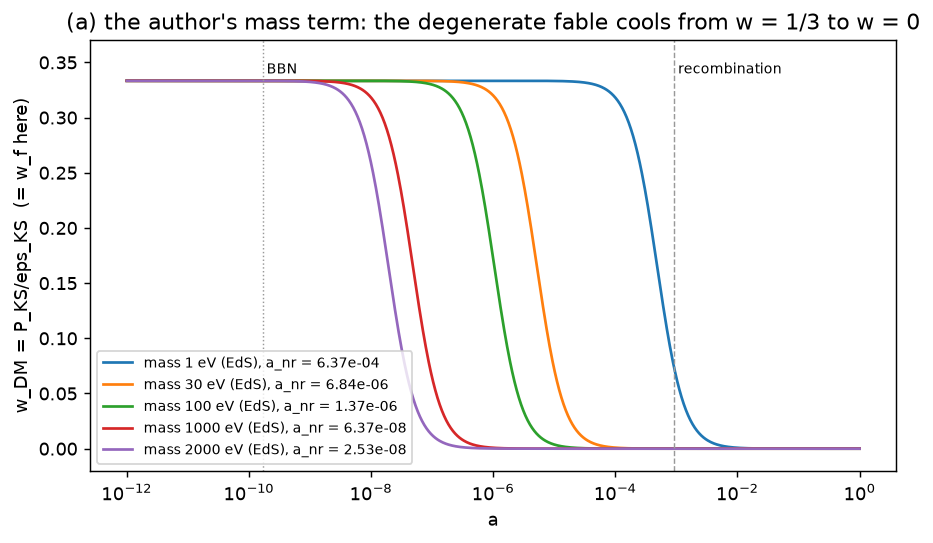
\includegraphics[width=0.75\linewidth]{nb06_a_mass_wdm.png}
  \caption{\texttt{fable-cosmology/\allowbreak results/\allowbreak nb06\_a\_mass\_wdm.png} (notebook 06, section 5.2), runs (a): the
  author's mass term, $\wDM=\PKS/\epsKS$ ($=w_f$ there) against $a$: the degenerate fable cools from $1/3$
  to 0.}
  \label{fig:nb06a}
\end{figure}

\subsubsection{Runs (b): a mass term plus a bare cosmological constant --- \texorpdfstring{$\Lambda$}{Lambda}CDM with fable dark matter}
\label{sec:4.7.5}

$W=V_0+m_0\sigma$, \texttt{fable4d}, $\Omegaqp=0.265$, $V_0$ (a bare Lambda) closing the budget \cfnb{nb06
\S5.3, figure \file{results/nb06_b_lambda_mass.png}} (figure~\ref{fig:nb06b}):

\begin{landscape}
{\scriptsize
\setlength{\tabcolsep}{4pt}
\begin{longtable}{@{}llllllllll@{}}
\toprule
run & $\anr$ & $\DNeff$ BBN & $\DNeff$ rec & CPL $w_f$ $(w_0,w_a)$ & CPL $\wDE$ $(w_0,w_a)$ & $\max|\wDE+1|$, $a\geq0.3$ & $q_0$ & $t_0$ [Gyr] & $V_0=\rho_U$ \tabularnewline
\midrule
\endhead
lambda-mass 30 eV & \texttt{4.4658e-06} & \texttt{0.07179} & \texttt{19.65} & \texttt{(-0.7573, +1.0100)} & \texttt{(-1.0000000003, +1.33e-09)} & \texttt{1.47e-09} & \texttt{-0.52845} & \texttt{13.8000} & \texttt{0.685665} \tabularnewline
lambda-mass 100 eV & \texttt{8.9687e-07} & \texttt{0.01442} & \texttt{19.65} & \texttt{(-0.7573, +1.0100)} & \texttt{(-1.0000000000, +5.34e-11)} & \texttt{5.91e-11} & \texttt{-0.52845} & \texttt{13.8000} & \texttt{0.685665} \tabularnewline
lambda-mass 1000 eV & \texttt{4.1629e-08} & \texttt{0.0006692} & \texttt{19.65} & \texttt{(-0.7573, +1.0100)} & \texttt{(-1.0000000000, +1.16e-13)} & \texttt{1.31e-13} & \texttt{-0.52845} & \texttt{13.8000} & \texttt{0.685665} \tabularnewline
lambda-mass 2000 eV & \texttt{1.6521e-08} & \texttt{0.0002656} & \texttt{19.65} & \texttt{(-0.7573, +1.0100)} & \texttt{(-1.0000000000, +1.72e-14)} & \texttt{2.40e-14} & \texttt{-0.52845} & \texttt{13.8000} & \texttt{0.685665} \tabularnewline
lambda-mass 30 eV (reference) & \texttt{4.4658e-06} & \texttt{0.07179} & \texttt{19.65} & \texttt{(-0.7569, +1.0092)} & \texttt{(-1.0000000003, +1.31e-09)} & \texttt{1.44e-09} & \texttt{-0.52845} & \texttt{13.8000} & \texttt{0.685665} \tabularnewline
\bottomrule
\end{longtable}
}
\end{landscape}

The mass does not vary ($\wDMeff=\wDM$, $Q=0$) and the condensate is the constant $V_0$, so the dark energy an
observer infers \textbf{is a cosmological constant}, to the precision of the quasiparticles' kinetic energy
that the observer counts as dark energy. The intrinsic $w_f$ today is \texttt{-0.72124767} [file:
\file{nb06_runs.csv}] --- it mixes the gas and $V_0$ and is not a dark-energy equation of state. The fifth run
($a_i=10^{-10}$, 701 rows, \file{results/nb06_fable4d_mass30eV.csv}) is Part~VIII's reference case
(\secref{sec:4.7.12}).

\begin{figure}[htbp]
  \centering
  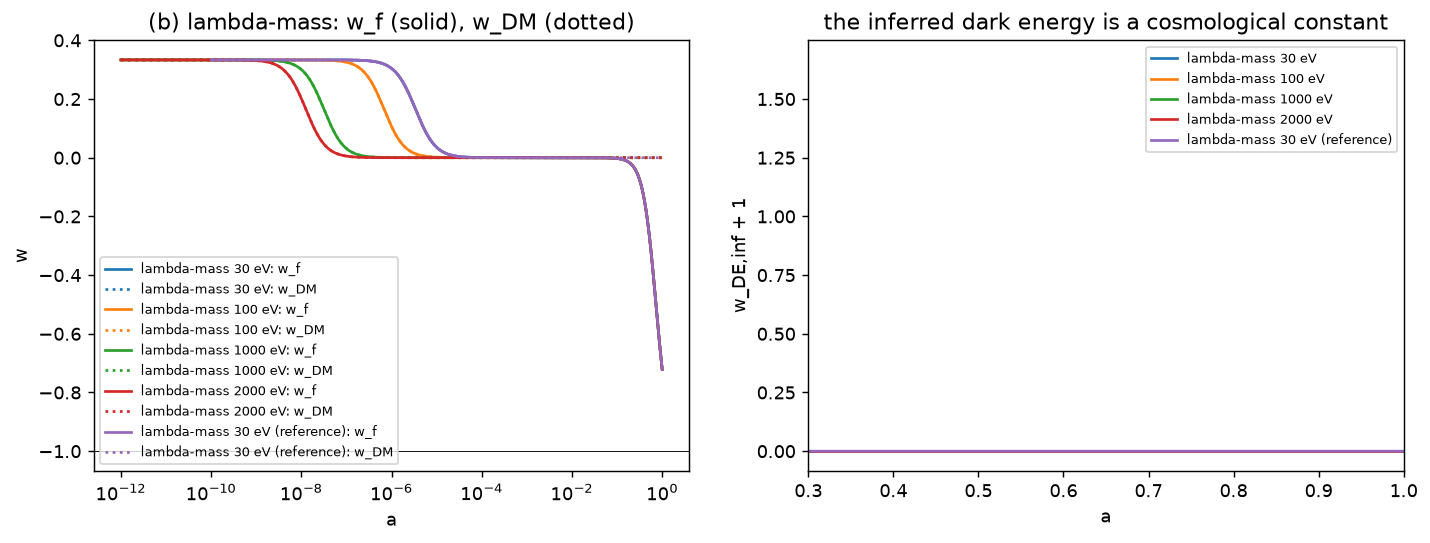
\includegraphics[width=0.95\linewidth]{nb06_b_lambda_mass.png}
  \caption{\texttt{fable-cosmology/\allowbreak results/\allowbreak nb06\_b\_lambda\_mass.png} (notebook 06, section 5.3), runs (b): $w_f$
  (solid) and $\wDM$ (dotted); and $\wDE+1$ on $0.3\leq a\leq1$: the inferred dark energy is a
  cosmological constant.}
  \label{fig:nb06b}
\end{figure}

\subsubsection{Runs (c): potentials with which the fable supplies the dark energy itself}
\label{sec:4.7.6}

\cfcode{power} ($\nu=0.236$, $0.5$), \cfcode{expdamp} (Part~VI's $x_t=1/2.21$), attractive \cfcode{quadratic}
($g_q=-0.5$), each at $\mtoday=30$ and $100$\,eV, \texttt{fable4d}, and Part~VIII's mass-varying reference case
(\cfcode{power}, $\nu=0.5$, $\mtoday=100$\,eV, $\Omegaqp=0.55$, 701 rows, \file{results/nb06_fable4d_power.csv})
\cfnb{nb06 \S5.4, figures \file{results/nb06_c_de_potentials.png},
\file{results/nb06_c_exchange_vacuum_stabilizer.png}} (figures~\ref{fig:nb06c1} and~\ref{fig:nb06c2}):

\begin{landscape}
{\scriptsize
\setlength{\tabcolsep}{3pt}
\begin{longtable}{@{}>{\raggedright\arraybackslash}p{0.11\linewidth}lllllllllll@{}}
\toprule
run & $\anr$ & \parbox[t]{1.6cm}{\raggedright min $m/\mtoday$ ($10^{-3}\leq a\leq0.3$)} & $w_f(1)$ & min $w_f$ & CPL $w_f$ & poles of $\wDE$ & $w=-1$ crossings & \parbox[t]{1.5cm}{\raggedright phantom in $0.3\leq a\leq1$?} & CPL $\wDE$ & fit from $a$ & min $c_s^2$ \tabularnewline
\midrule
\endhead
power nu=0.236, 30 eV & \texttt{2.22e-05} & \texttt{2.01e-01} & \texttt{-0.7212} & \texttt{-0.7212} & \texttt{(-0.783, +0.445)} & \texttt{3.43e-06, 0.533} & \texttt{4.55966e-06, 1} & True & \texttt{(-0.082, -7.986)} & \texttt{0.559} & \texttt{-0.611} \tabularnewline
power nu=0.236, 100 eV & \texttt{4.47e-06} & \texttt{2.01e-01} & \texttt{-0.7212} & \texttt{-0.7212} & \texttt{(-0.783, +0.445)} & \texttt{6.89e-07, 0.533} & \texttt{9.15884e-07, 1} & True & \texttt{(-0.082, -7.986)} & \texttt{0.559} & \texttt{-0.611} \tabularnewline
power nu=0.5, 30 eV & \texttt{0.669} & \texttt{7.91e-12} & \texttt{-0.7212} & \texttt{-1.0000} & \texttt{(-0.804, -0.358)} & \texttt{3.35e-06, 0.619} & \texttt{4.46748e-06, 1} & True & \texttt{(-0.249, -10.191)} & \texttt{0.650} & \texttt{-27} \tabularnewline
power nu=0.5, 100 eV & \texttt{0.669} & \texttt{1.59e-12} & \texttt{-0.7212} & \texttt{-1.0000} & \texttt{(-0.804, -0.359)} & \texttt{6.73e-07, 0.619} & \texttt{8.97015e-07, 1} & True & \texttt{(-0.249, -10.191)} & \texttt{0.650} & \texttt{-27} \tabularnewline
expdamp xt=1/2.21, 30 eV & \texttt{0.712} & \texttt{6.58e-12} & \texttt{-0.7212} & \texttt{-1.0000} & \texttt{(-0.829, -0.317)} & \texttt{3.35e-06, 0.625} & \texttt{4.46748e-06, 1} & True & \texttt{(-0.128, -11.778)} & \texttt{0.656} & \texttt{-21.8} \tabularnewline
expdamp xt=1/2.21, 100 eV & \texttt{0.712} & \texttt{1.32e-12} & \texttt{-0.7212} & \texttt{-1.0000} & \texttt{(-0.829, -0.317)} & \texttt{6.73e-07, 0.625} & \texttt{8.97015e-07, 1} & True & \texttt{(-0.128, -11.779)} & \texttt{0.656} & \texttt{-21.8} \tabularnewline
quadratic gq=$-$0.5, 30 eV & \texttt{0.643} & \texttt{8.93e-12} & \texttt{-0.7212} & \texttt{-1.0000} & \texttt{(-0.730, -0.483)} & \texttt{3.35e-06, 0.602} & \texttt{4.46748e-06, 1} & True & \texttt{(-0.180, -9.321)} & \texttt{0.632} & \texttt{-47.1} \tabularnewline
quadratic gq=$-$0.5, 100 eV & \texttt{0.643} & \texttt{1.79e-12} & \texttt{-0.7212} & \texttt{-1.0000} & \texttt{(-0.730, -0.483)} & \texttt{6.73e-07, 0.602} & \texttt{8.97015e-07, 1} & True & \texttt{(-0.180, -9.321)} & \texttt{0.632} & \texttt{-47.1} \tabularnewline
power nu=0.5, 100 eV, $\Omegaqp=0.55$ & \texttt{4.21e-06} & \texttt{2.72e-01} & \texttt{-0.4215} & \texttt{-0.4215} & \texttt{(-0.448, +0.264)} & \texttt{8.96e-07, 0.63} & \texttt{1.18957e-06, 1} & True & \texttt{(-0.327, -9.682)} & \texttt{0.662} & \texttt{-0.364} \tabularnewline
\bottomrule
\end{longtable}
}

\noindent and, for the same runs \cfnb{nb06 \S5.4}:

{\scriptsize
\setlength{\tabcolsep}{5pt}
\begin{longtable}{@{}llllll@{}}
\toprule
run & $c_s^2<0$ on ($a\geq10^{-3}$) & $\wDMeff$ range ($a\geq10^{-3}$) & $|\Evac|/\rho_{\mathrm{tot}}$, $a\geq0.3$ & $\Pstab(1)$ [$\rhoc$] & $\DNeff$ BBN \tabularnewline
\midrule
\endhead
power nu=0.236, 30 eV & \texttt{[0.00409, 1]} & \texttt{(-0.611, +9.85e-05)} & \texttt{1.314e+13} & \texttt{-0.8428} & \texttt{0.0718} \tabularnewline
power nu=0.236, 100 eV & \texttt{[0.00194, 1]} & \texttt{(-0.611, +3.59e-06)} & \texttt{1.622e+15} & \texttt{-0.8428} & \texttt{0.0144} \tabularnewline
power nu=0.5, 30 eV & \texttt{[0.608, 1]} & \texttt{(-27.6, +0.333)} & \texttt{2.229e+14} & \texttt{-0.8428} & \texttt{0.0718} \tabularnewline
power nu=0.5, 100 eV & \texttt{[0.608, 1]} & \texttt{(-27.7, +0.333)} & \texttt{2.752e+16} & \texttt{-0.8428} & \texttt{0.0144} \tabularnewline
expdamp xt=1/2.21, 30 eV & \texttt{[0.643, 1]} & \texttt{(-21.8, +0.333)} & \texttt{2.327e+14} & \texttt{-0.8428} & \texttt{0.0718} \tabularnewline
expdamp xt=1/2.21, 100 eV & \texttt{[0.643, 1]} & \texttt{(-21.8, +0.333)} & \texttt{2.873e+16} & \texttt{-0.8428} & \texttt{0.0144} \tabularnewline
quadratic gq=$-$0.5, 30 eV & \texttt{[0.592, 1]} & \texttt{(-47.1, +0.333)} & \texttt{2.031e+14} & \texttt{-0.8428} & \texttt{0.0718} \tabularnewline
quadratic gq=$-$0.5, 100 eV & \texttt{[0.592, 1]} & \texttt{(-47.1, +0.333)} & \texttt{2.508e+16} & \texttt{-0.8428} & \texttt{0.0144} \tabularnewline
power nu=0.5, 100 eV, $\Omegaqp=0.55$ & \texttt{[0.001, 1]} & \texttt{(-0.364, -3.89e-05)} & \texttt{2.350e+14} & \texttt{-0.7003} & \texttt{0.0382} \tabularnewline
\bottomrule
\end{longtable}
}
\end{landscape}

\noindent and
\cfcode{smallest w_f over all 9 runs: -0.9999987921 (never below -1);  every run has c_s^2 < 0 somewhere after a = 1e-3: True}.
Reading the tables:
\begin{itemize}
  \item Only the two $\nu=0.236$ runs and the reference run stay \textbf{massive} through the matter era. The
        $\nu=0.5$, \cfcode{expdamp} and \cfcode{quadratic} runs with $\Omegaqp=0.265$ have
        $\min m/\mtoday\sim10^{-12}$: the gap pins their mass near zero and the fable is a \textbf{massless
        gas} (radiation, $w=1/3$) until $\anr=0.64$--$0.71$ --- it supplies no dark matter at recombination
        ($\DNeff$ at recombination equals its BBN value, e.g.\ \texttt{0.071792425} for
        \cfcode{power nu=0.5, 30 eV} [file: \file{nb06_runs.csv}]). Their CPL fits of $w_f$ look like the
        supernova fits $(-0.861,-0.60)$, but they are not viable cosmologies.
  \item The observer's inferred dark energy $\wDE$ has \textbf{poles} (its $\rhoDE$ changes sign) inside
        $0.3\leq a\leq1$ in every run, and it is phantom and crosses $-1$ in every run; a CPL line is not a
        faithful description (the fits above the pole are in \file{results/nb06_cpl_fits.csv}).
  \item $c_s^2<0$ in every run: an \textbf{adiabatic instability}.
  \item The Dirac-sea energy that the no-sea functional drops changes along every run by
        $1.31\times10^{13}$ to $2.87\times10^{16}$ times the total density at $a\geq0.3$.
\end{itemize}

\begin{figure}[htbp]
  \centering
  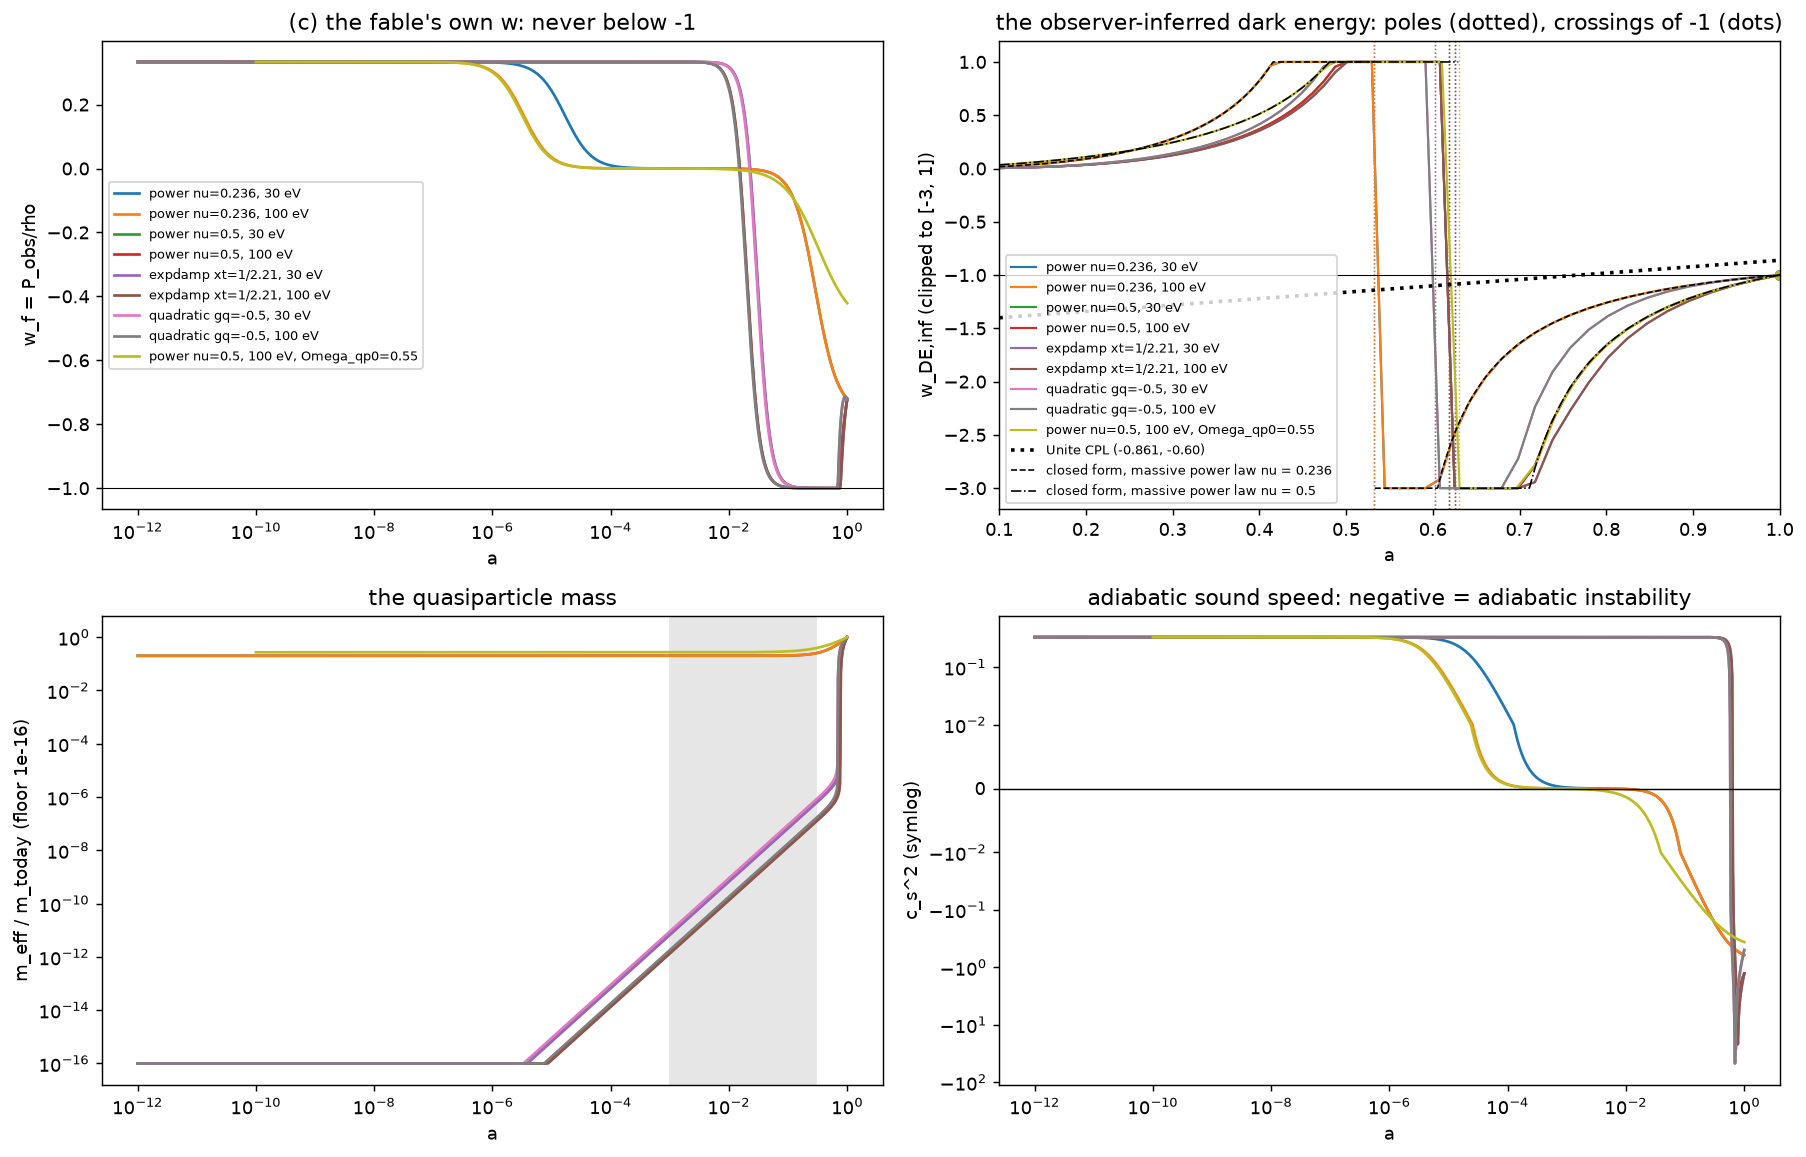
\includegraphics[width=0.95\linewidth]{nb06_c_de_potentials.png}
  \caption{\texttt{fable-cosmology/\allowbreak results/\allowbreak nb06\_c\_de\_potentials.png} (notebook 06, section 5.4), runs (c):
  $w_f$ (never below $-1$), the observer's $\wDE$ (clipped to $[-3,1]$, poles and crossings marked),
  $\meffx/\mtoday$, and $c_s^2$ (negative below the line).}
  \label{fig:nb06c1}
\end{figure}
\begin{figure}[htbp]
  \centering
  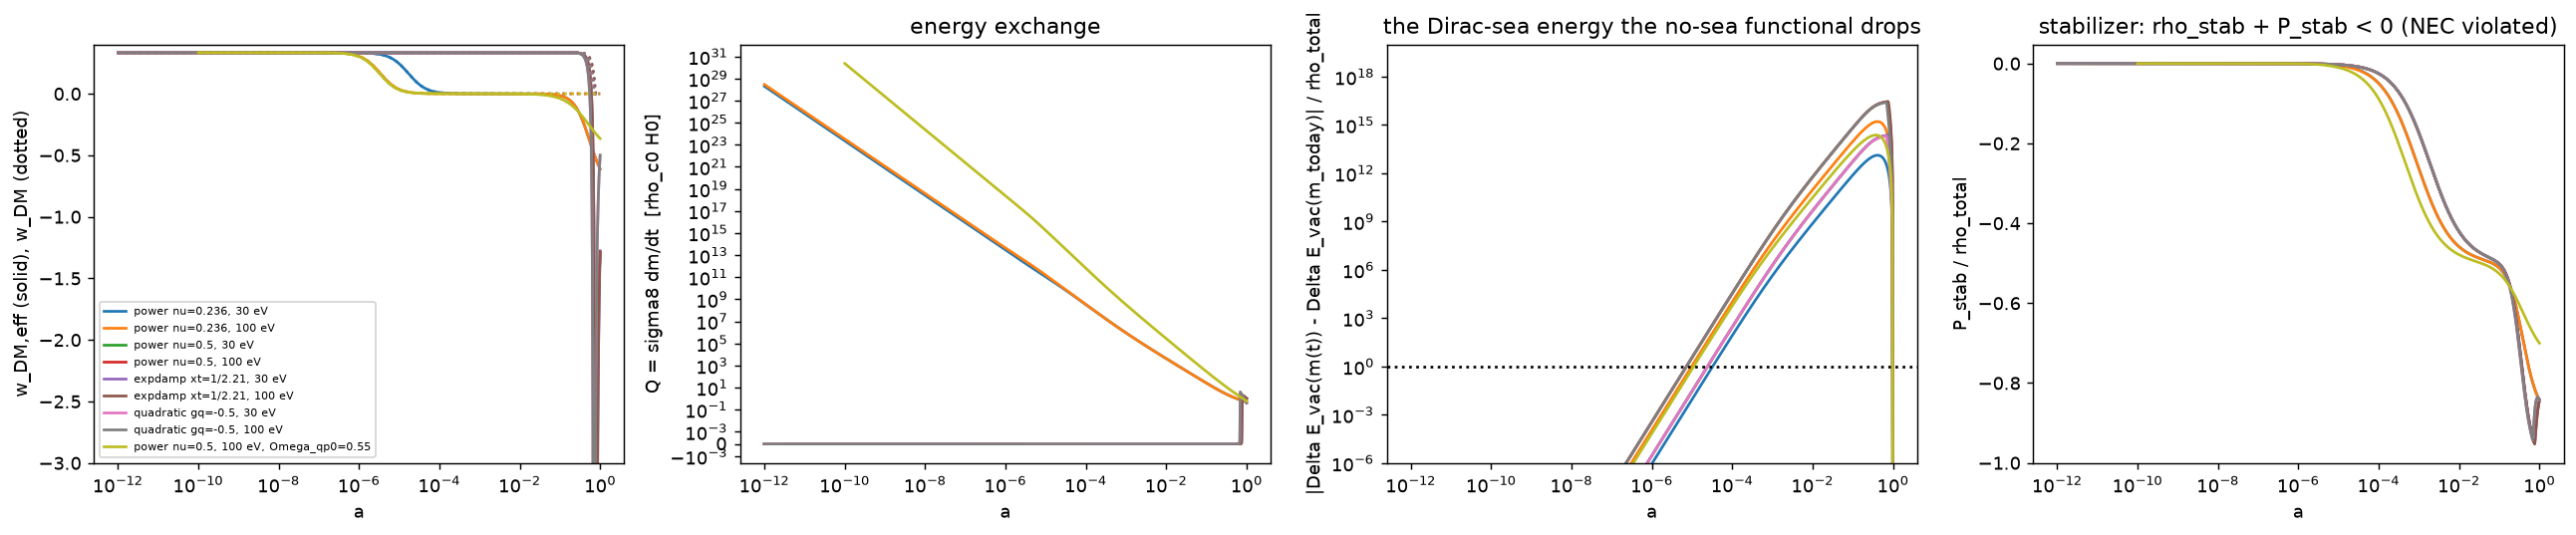
\includegraphics[width=\linewidth]{nb06_c_exchange_vacuum_stabilizer.png}
  \caption{\texttt{fable-cosmology/\allowbreak results/\allowbreak nb06\_c\_exchange\_vacuum\_stabilizer.png} (notebook 06, section 5.4),
  runs (c): $\wDM$ and $\wDMeff$, the exchange $Q$, the Dirac-sea energy relative to the total density, and
  $\Pstab/\rho$.}
  \label{fig:nb06c2}
\end{figure}

\subsubsection{The inferred dark energy of a massive power law, in closed form}
\label{sec:4.7.7}

Once the gas is non-relativistic, $\sigma_8\approx n\propto a^{-3}$, the condensate is $U=U_t\,a^{-3\nu}$ and the
mass $m(a)=m_0+\nu\,U_t\,a^{3(1-\nu)}/\bigl((1-\nu)\,\sigma_t\bigr)$. Subtracting cold dark matter with today's
mass leaves $\rhoDE=U+\bigl(m(a)-\mtoday\bigr)\,n=U_t\bigl[a^{-3\nu}-\nu\,a^{-3}\bigr]/(1-\nu)$ and $P_{\mathrm{DE}}=-U$,
hence
\[
  \wDE(a)=-\frac{1-\nu}{1-\nu\,a^{-3(1-\nu)}} ,
\]
a pole at $a_{\mathrm{pole}}=\nu^{1/(3(1-\nu))}$, $w>0$ before it, phantom ($w<-1$) between it and today, and
$w=-1$ at $a=1$ up to the quasiparticles' kinetic energy, which makes it cross $-1$ just before today. It
depends on $\nu$ alone [prose nb06 \S5.4]. The runs agree \cfnb{nb06 \S5.4}:
\begin{Verbatim}[fontsize=\scriptsize]
power nu=0.236, 30 eV                  w_DE,inf against -(1-nu)/(1 - nu a^(-3(1-nu))) on a >= 0.3: max deviation 1.2e-09;  pole: formula 0.532600, run 0.532723;  crossing of -1: 1.00000000
power nu=0.236, 100 eV                 w_DE,inf against -(1-nu)/(1 - nu a^(-3(1-nu))) on a >= 0.3: max deviation 4.9e-11;  pole: formula 0.532600, run 0.532723;  crossing of -1: 1.00000000
power nu=0.5, 100 eV, Omega_qp0=0.55   w_DE,inf against -(1-nu)/(1 - nu a^(-3(1-nu))) on a >= 0.3: max deviation 4.2e-11;  pole: formula 0.629961, run 0.630028;  crossing of -1: 1.00000000
\end{Verbatim}
The mechanism is that of Das, Corasaniti and Khoury, Phys.\ Rev.\ D \textbf{73}, 083509 (2006): subtracting
cold dark matter with today's mass when the mass was different leaves
$\rho_{\mathrm{DE}}+P_{\mathrm{DE}}\approx\bigl(\meffx(a)-\mtoday\bigr)\,n$, which is negative whenever $\meffx$
grows; an apparent phantom with no phantom field.

\subsubsection{The scans: where does a dark-energy fable stay massive through the matter era?}
\label{sec:4.7.8}

Notebook 06 scanned the shape parameters --- \cfcode{power} $\nu=0.05\dots0.65$, \cfcode{quadratic}
$g_q=-0.95\dots-0.05$, \cfcode{expdamp} $x_t=0.1\dots0.9$, and for \cfcode{power} $\nu=0.3$ and $0.5$ the
quasiparticle share $\Omegaqp=0.265\dots0.8$ --- at $\mtoday=1000$\,eV and $100$\,eV (\texttt{fable4d}, 401
output rows, $45+45$ runs), and re-computed every scan run independently as it ran \cfnb{nb06 \S5.6, files
\file{results/nb06_scan.csv}, figures \file{results/nb06_scan.png}, \file{results/nb06_scan_cpl.png}}
(figures~\ref{fig:nb06scan} and~\ref{fig:nb06scancpl}). Its conclusions, verbatim:
\begin{Verbatim}[fontsize=\scriptsize]
scan points whose fable stays massive through 1e-3 <= a <= 0.3 (min m/m_today > 1e-3): 28 of 90: power, nu=0.05 (1000 eV), power, nu=0.1 (1000 eV), power, nu=0.15 (1000 eV), power, nu=0.2 (1000 eV), power, nu=0.25 (1000 eV), power nu=0.3, Omega_qp0=0.35 (1000 eV), power nu=0.3, Omega_qp0=0.45 (1000 eV), power nu=0.3, Omega_qp0=0.55 (1000 eV), power nu=0.3, Omega_qp0=0.65 (1000 eV), power nu=0.3, Omega_qp0=0.8 (1000 eV), power nu=0.5, Omega_qp0=0.5 (1000 eV), power nu=0.5, Omega_qp0=0.55 (1000 eV), power nu=0.5, Omega_qp0=0.65 (1000 eV), power nu=0.5, Omega_qp0=0.8 (1000 eV), power, nu=0.05 (100 eV), power, nu=0.1 (100 eV), power, nu=0.15 (100 eV), power, nu=0.2 (100 eV), power, nu=0.25 (100 eV), power nu=0.3, Omega_qp0=0.35 (100 eV), power nu=0.3, Omega_qp0=0.45 (100 eV), power nu=0.3, Omega_qp0=0.55 (100 eV), power nu=0.3, Omega_qp0=0.65 (100 eV), power nu=0.3, Omega_qp0=0.8 (100 eV), power nu=0.5, Omega_qp0=0.5 (100 eV), power nu=0.5, Omega_qp0=0.55 (100 eV), power nu=0.5, Omega_qp0=0.65 (100 eV), power nu=0.5, Omega_qp0=0.8 (100 eV)
of these, with c_s^2 >= 0 after a = 1e-3: 0;  smallest c_s^2 among them: -0.6469;  largest: -0.0565
power law: 'massive through the matter era' <=> 'bare m0 > 0' at all 52 power scan points: True
the estimate Omega_qp0/U_t > nu/(1 - nu) agrees with the sign of m0 at 52 of 52 points;  with Omega_qp0 = 0.265 it allows nu < Omega_qp0/(1 - Omega_b0 - Omega_r0) = 0.2788
\end{Verbatim}
So: \textbf{every \cfcode{quadratic} and \cfcode{expdamp} point is massless in the matter era; a power law
stays massive exactly when its bare mass $m_0=\mtoday-\nu\lambda\sigma_t^{\nu-1}$ is positive, i.e.\ when
$\Omegaqp/U_t>\nu/(1-\nu)$; with the observed split $\Omegaqp=0.265$ that requires $\nu<0.2788$} (massive up to
$\nu=0.25$, massless from $\nu=0.3$ in the scan); a larger $\nu$ needs a larger quasiparticle share
($\Omegaqp\geq0.35$ for $\nu=0.3$, $\geq0.5$ for $\nu=0.5$). And every massive point has $c_s^2<0$ after
$a=10^{-3}$. (At high density $\nu\lambda\sigma^{\nu-1}\to0$, so if $m_0<0$ the gap can only be met with $m\to0^+$;
with $\sigma_t\approx n_t$ and $\epsKS\approx\mtoday\,n_t$ today this happens exactly when
$\Omegaqp/U_t<\nu/(1-\nu)$ [prose nb06 \S5.6].) In the massless cases the smallest $c_s^2$ sits at the sharp
release of the pinned gap, and its magnitude depends on how finely the output grid samples that release; its
sign does not [prose nb06 \S5.6]. The largest cross-check difference over the 90 scan runs is
\texttt{4.43e-09} \cfnb{nb06 \S5.10}.

\begin{figure}[htbp]
  \centering
  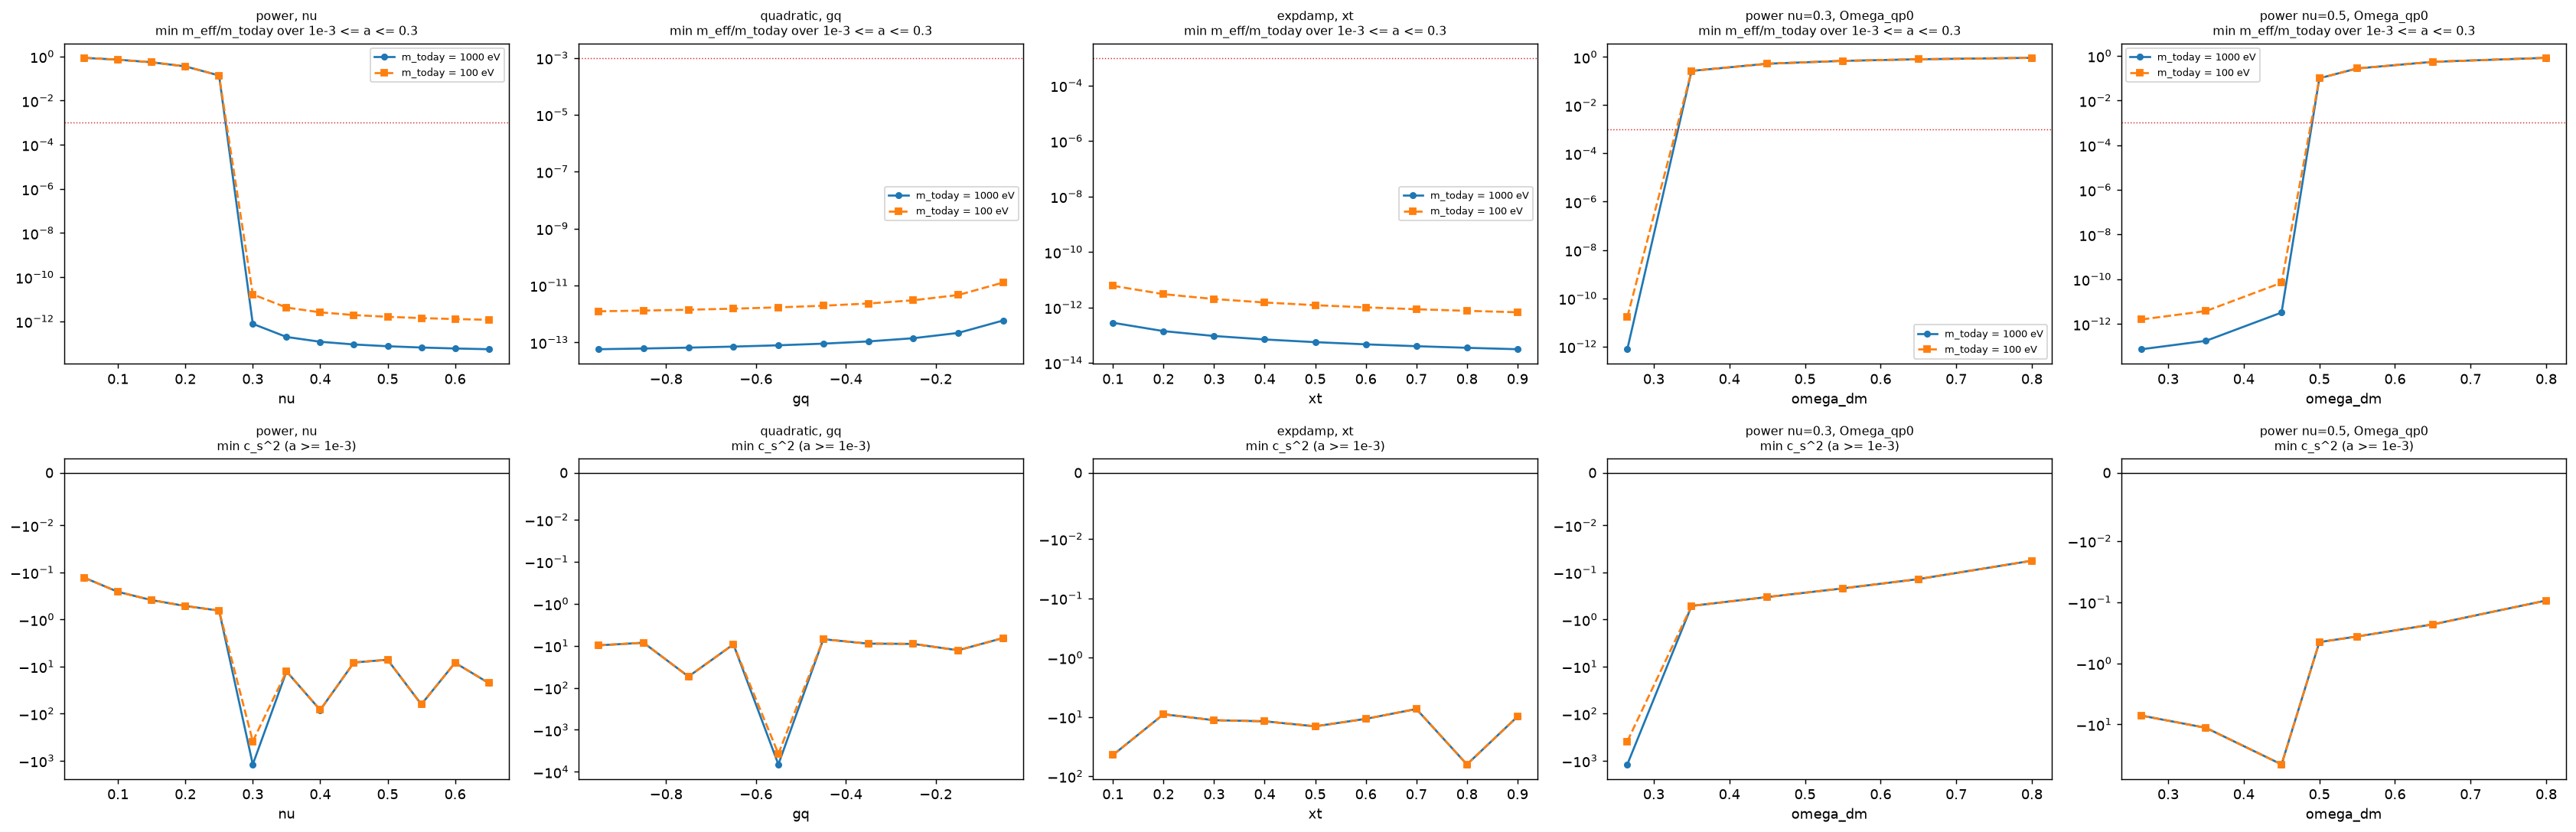
\includegraphics[width=\linewidth]{nb06_scan.png}
  \caption{\texttt{fable-cosmology/\allowbreak results/\allowbreak nb06\_scan.png} (notebook 06, section 5.6), the scans: per family, the
  smallest $\meffx/\mtoday$ over $10^{-3}\leq a\leq0.3$ and the smallest $c_s^2$ ($a\geq10^{-3}$) against the
  scanned parameter.}
  \label{fig:nb06scan}
\end{figure}
\begin{figure}[htbp]
  \centering
  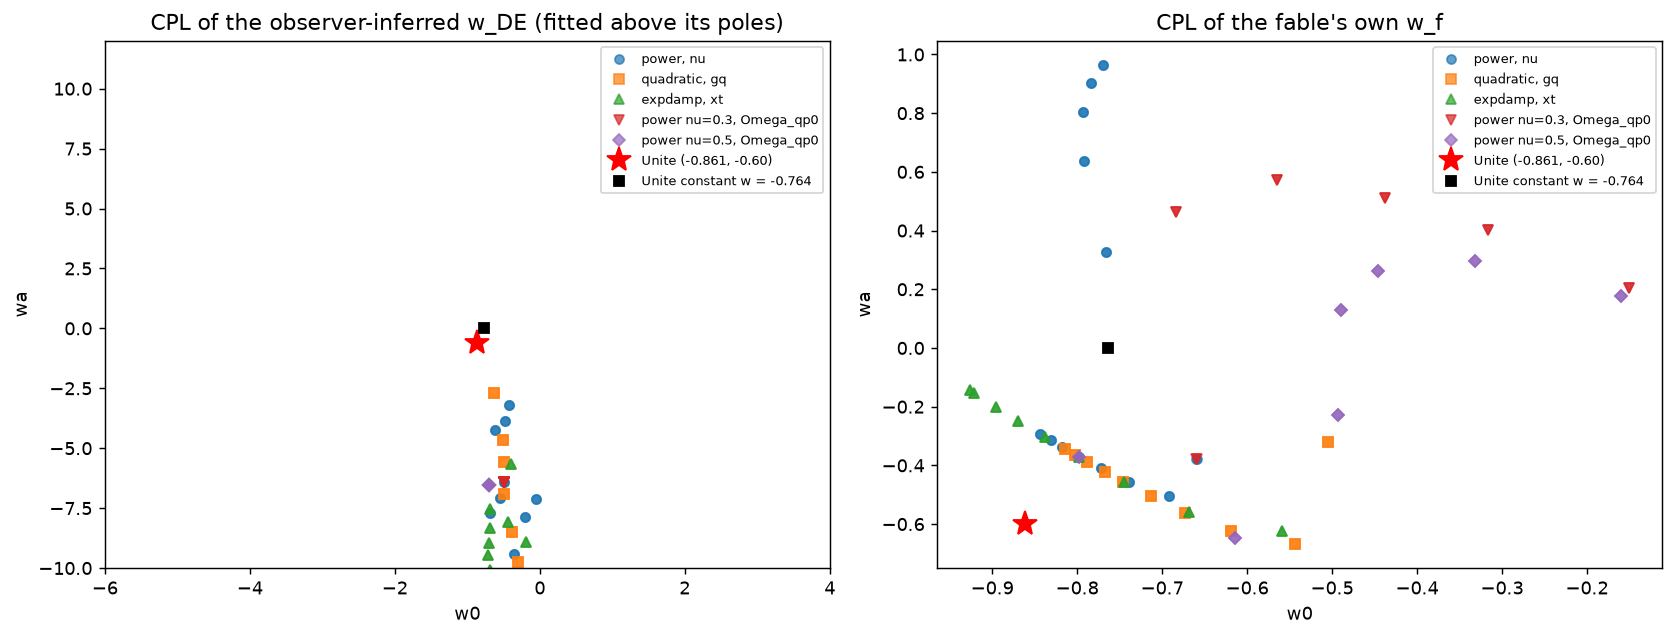
\includegraphics[width=0.95\linewidth]{nb06_scan_cpl.png}
  \caption{\texttt{fable-cosmology/\allowbreak results/\allowbreak nb06\_scan\_cpl.png} (notebook 06, section 5.6), the scans: the CPL
  points $(w_0,w_a)$ of $\wDE$ (fitted above its poles) and of $w_f$.}
  \label{fig:nb06scancpl}
\end{figure}

\subsubsection{How heavy must a fable that is all of the dark matter be?}
\label{sec:4.7.9}

\cfnb{nb06 \S5.7, file \file{results/nb06_dm_mass_bounds.csv}, figure \file{results/nb06_dm_mass_bounds.png}}
(figure~\ref{fig:nb06dm})

{\small
\renewcommand{\arraystretch}{1.3}
\begin{longtable}{@{}>{\raggedright\arraybackslash}p{0.36\linewidth}>{\raggedright\arraybackslash}p{0.17\linewidth}>{\raggedright\arraybackslash}p{0.41\linewidth}@{}}
\toprule
bound & fable mass & detail \tabularnewline
\midrule
\endhead
$\DNeff(\mathrm{BBN})<0.3$ & $m>10.2645$\,eV & fit over 17 runs: $\DNeff=6.6922\,(m/\mathrm{eV})^{-1.33333}$, max $|\ln\text{residual}|=$ \texttt{7.1e-05} \tabularnewline
$\DNeff(\mathrm{BBN})<0.2$ & $m>13.9126$\,eV & same fit \tabularnewline
free streaming: $v_{\mathrm{rms}0}$ matched to thermal WDM of 3.3\,keV (Viel et al.\ 2013) & $m\approx1124.92$\,eV & $v_{\mathrm{rms}0}=$ \texttt{8.2629e-03} km/s \tabularnewline
free streaming: $v_{\mathrm{rms}0}$ matched to thermal WDM of 5.3\,keV (Ir\v{s}i\v{c} et al.\ 2017) & $m\approx1806.69$\,eV & $v_{\mathrm{rms}0}=$ \texttt{4.3932e-03} km/s \tabularnewline
Tremaine--Gunn, $g=8$, $\sigma=10$\,km/s, $r_c=0.3$\,kpc & $m>231.315$\,eV & $m^4>9\,h^3/\bigl(2\,(2\pi)^{5/2}\,g\,G\,\sigma\,r_c^2\bigr)$ \tabularnewline
Tremaine--Gunn, $g=8$, $\sigma=7$\,km/s, $r_c=0.15$\,kpc & $m>357.639$\,eV & same \tabularnewline
\bottomrule
\end{longtable}
}

\noindent$\DNeff\propto m^{-4/3}$ because $\DNeff(\mathrm{BBN})$ depends only on $k_{F0}$, which
$\epsKS(m,k_{F0})=\Omegaqp$ fixes, and $k_{F0}\propto m^{-1/3}$ for a non-relativistic gas today; at 1, 30, 100,
1000, 2000\,eV it is \texttt{6.69227}, \texttt{0.0717924}, \texttt{0.0144181}, \texttt{0.000669238},
\texttt{0.00026561}. A degenerate gas has the velocity dispersion of a filled Fermi sphere,
$v_{\mathrm{rms}}=\sqrt{3/5}\,\kF/m$: \texttt{4.4870e+00}, \texttt{2.6132e+00}, \texttt{2.0827e-01},
\texttt{9.6670e-03}, \texttt{3.8364e-03} km/s at 10, 15, 100, 1000, 2000\,eV. The Lyman-alpha-allowed
thermal-relic warm dark matter ($m_{\mathrm{WDM}}\gtrsim3.3$\,keV and 5.3\,keV) has $v_{\mathrm{rms}0}=$
\texttt{8.2629e-03} and \texttt{4.3932e-03} km/s; a degenerate fable with the same $v_{\mathrm{rms}0}$ needs
$m\approx1.1$--$1.8$\,keV --- a velocity-matching estimate, not a transfer-function computation. The
Tremaine--Gunn bound uses illustrative dwarf-spheroidal values (inputs, not results). The free-streaming
bound is far stronger than $\DNeff$. At such masses the change of $\wDM$ from $1/3$ to 0 happens around
$\anr=4.16\times10^{-8}$ (1\,keV) or $1.65\times10^{-8}$ (2\,keV).

\begin{figure}[htbp]
  \centering
  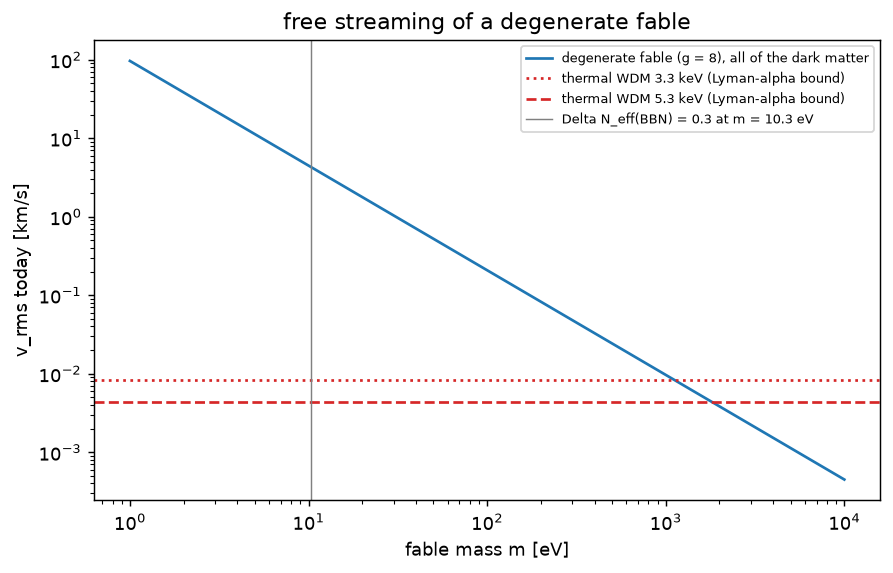
\includegraphics[width=0.75\linewidth]{nb06_dm_mass_bounds.png}
  \caption{\texttt{fable-cosmology/\allowbreak results/\allowbreak nb06\_dm\_mass\_bounds.png} (notebook 06, section 5.7): the free
  streaming of a degenerate fable: $v_{\mathrm{rms}}$ today against the fable mass, with the warm-dark-matter
  velocities.}
  \label{fig:nb06dm}
\end{figure}

\subsubsection{Runs (d): without the stabilizer, the hidden sheet moves and the Newton constant varies}
\label{sec:4.7.10}

\texttt{fable8d} for the mass term at 1 and 100\,eV and \cfcode{lambda-mass} at 30\,eV and 1\,keV, and two
controls: radiation alone (\cfcode{--no-fable --omega-b 0}), which must keep the hidden sheet exactly frozen
($F=0$), and radiation plus baryons (\cfcode{--no-fable}), in which dust alone drives it.
$G(a)/G(1)=1/v$ (the observed Newton constant is $G_4=G_8/\Vhidx\propto1/v$) \cfnb{nb06 \S5.8, file
\file{results/nb06_nogo_8d.csv}, figure \file{results/nb06_d_nogo_8d.png}} (figure~\ref{fig:nb06d}):

\begin{landscape}
{\scriptsize
\setlength{\tabcolsep}{4pt}
\begin{longtable}{@{}>{\raggedright\arraybackslash}p{0.13\linewidth}*{10}{>{\raggedright\arraybackslash}p{0.072\linewidth}}@{}}
\toprule
run & $B(a_i)=C(a_i)$ & $G(a_i)/G(1)$ & $G(\mathrm{BBN})/G(1)$ & $\Delta G/G$ since BBN & $|d\ln G/dt|$ today [/yr] & $H_B/H_A(1)={}$ $H_C/H_A(1)$ & max constraint residual & $\Omega_{\mathrm{sum}}(1)$ & $q_0$ & $t_0$ [Gyr] \tabularnewline
\midrule
\endhead
mass 1 eV, fable8d & \texttt{2.3224e-03} & \texttt{3.4376e+10} & \texttt{3.4376e+10} & \texttt{-1.0000e+00} & \texttt{2.7571e-10} & \texttt{0.999959} & \texttt{1.16e-08} & \texttt{6.99967} & \texttt{2.5000} & \texttt{4.145} \tabularnewline
mass 100 eV, fable8d & \texttt{4.8207e-05} & \texttt{1.8516e+17} & \texttt{1.8516e+17} & \texttt{-1.0000e+00} & \texttt{2.7571e-10} & \texttt{0.999963} & \texttt{2.12e-08} & \texttt{6.99971} & \texttt{2.5000} & \texttt{4.145} \tabularnewline
lambda-mass 30 eV, fable8d & \texttt{9.8881e-04} & \texttt{1.0461e+12} & \texttt{1.0461e+12} & \texttt{-1.0000e+00} & \texttt{2.7570e-10} & \texttt{0.999902} & \texttt{2.47e-08} & \texttt{6.99922} & \texttt{-0.8425} & \texttt{9.472} \tabularnewline
lambda-mass 1 keV, fable8d & \texttt{9.8389e-04} & \texttt{1.0671e+12} & \texttt{1.0671e+12} & \texttt{-1.0000e+00} & \texttt{2.7570e-10} & \texttt{0.999902} & \texttt{2.07e-08} & \texttt{6.99922} & \texttt{-0.8425} & \texttt{9.472} \tabularnewline
radiation only, fable8d & \texttt{1.0000e+00} & \texttt{1.0000e+00} & \texttt{1.0000e+00} & \texttt{0.0000e+00} & \texttt{0.0000e+00} & \texttt{0.000000} & \texttt{9.89e-16} & \texttt{1.00000} & \texttt{1.0000} & \texttt{755.851} \tabularnewline
radiation + baryons, fable8d & \texttt{6.2532e-03} & \texttt{6.5402e+08} & \texttt{6.5402e+08} & \texttt{-1.0000e+00} & \texttt{2.3096e-11} & \texttt{0.994782} & \texttt{1.04e-08} & \texttt{6.95831} & \texttt{2.4935} & \texttt{49.354} \tabularnewline
\bottomrule
\end{longtable}
}
\end{landscape}

Radiation alone keeps $H_B=H_C=0$ exactly (\cfcode{max |H_B/H_A| = 0.0e+00}: $F=0$); dust or vacuum energy drives
the hidden sheet to the 7-dimensional isotropic attractor ($H_B/H_A\to1$), and the observed Newton constant
changes by $\boldsymbol{6.5\times10^{8}}$ \textbf{to} $\boldsymbol{1.9\times10^{17}}$ between the start and
today, with $|d\ln G/dt|$ today $2.3\times10^{-11}$ to $2.76\times10^{-10}$\,/yr against the lunar-laser-ranging
bound $10^{-13}$\,/yr, and $\Delta G/G$ since nucleosynthesis $-1$ against the bound of about $0.1$. The closure
today then needs $\Omega_{\mathrm{sum}}(1)\approx7$
($\sum\Omega_i=1+\bigl(3H_B^2+9H_AH_B+3H_AH_C+3H_BH_C\bigr)/(3H_A^2)$, which is 7 on the attractor). The two
controls have nothing to shoot, so their $H_A$ today is not 1 and their ages are not those of our universe.
\textbf{\texttt{fable8d} is a no-go for observers; that is why the physical model is the stabilized
\texttt{fable4d}.} The last run, \cfcode{fable8d --freeze-hidden} (\cfcode{lambda-mass} 30\,eV), agrees with the
algebraic \texttt{fable4d}:
\cfcode{max |dH_A|/H_A = 4.1e-09, max |dt|/t = 9.8e-09, max |dw_f| = 0.0e+00, max |H_B| = 0.0e+00}.

\begin{figure}[htbp]
  \centering
  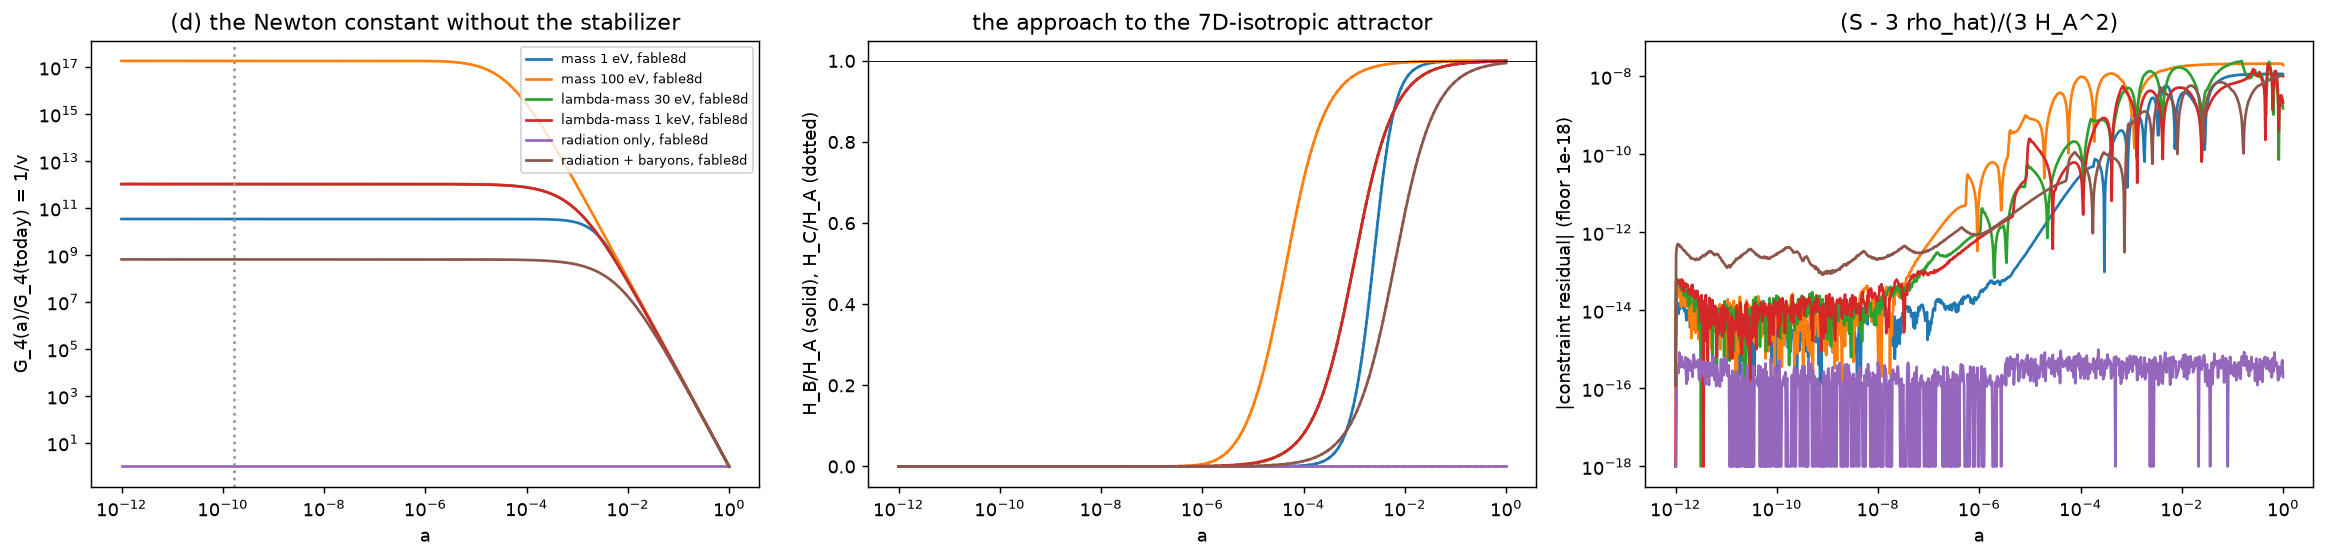
\includegraphics[width=\linewidth]{nb06_d_nogo_8d.png}
  \caption{\texttt{fable-cosmology/\allowbreak results/\allowbreak nb06\_d\_nogo\_8d.png} (notebook 06, section 5.8), runs (d):
  $G_4(a)/G_4(\text{today})=1/v$, $H_B/H_A$ and $H_C/H_A$ (the approach to the 7-dimensional isotropic
  attractor), and the constraint residual $(S-3\hat\rho)/(3H_A^2)$.}
  \label{fig:nb06d}
\end{figure}

\subsubsection{The cases the solver refuses, and why}
\label{sec:4.7.11}

Each exits with code 1 and one line of physical reason \cfnb{nb06 \S5.9}:
\begin{Verbatim}[fontsize=\scriptsize]
$ fable_fermion fable4d --potential lorentz --points 1001
  exit code 1: fable_fermion: rho_hat = H_A^2 <= 0 from N = -0.7597808064 (a = 0.4677689478) on: the Kohn-Sham ground state has negative energy there (m_eff = -3.802078e-2, sigma8 = -9.789374e-4, rho_f = -4.830421e-1 (U = -4.847891e-1) against rho_r + rho_b = 4.830421e-1); H_A^2 = rho_hat is impossible (the onset located past the last accepted CVODE step and bisected)
$ fable_fermion fable4d --potential quadratic --param gq=0.5 --points 1001
  exit code 1: fable_fermion: gap-branch jump at N = -0.0037262796 (a = 0.9962806544): a first-order transition of the Kohn-Sham ground state, the lowest-energy gap root jumps from the branch m_eff = -1.518260e0 (rho_f = 6.856759e-1) to the branch m_eff = 4.083552e2 (rho_f = 9.536521e-1); the right-hand side is discontinuous there, and energy conservation across it would need the Maxwell construction, which this solver does not implement (the transition detected inside the right-hand side and bisected in N to adjacent doubles)
$ fable_fermion fable8d --potential mass --direction backward
  exit code 1: fable_fermion: fable8d runs forward only (design review E4): backward in time the shear modes grow as A^-3 v^-1 relative to H_A ~ A^-2, the solution runs to the 8D Kasner point H_B/H_A = -0.2929 and the constraint drifts to O(1); use fable4d --direction backward
all three refused with exit code 1 and the expected reason
\end{Verbatim}
\cfcode{lorentz}: the Kohn--Sham ground state moves to the negative-$\sigma$ branch, whose energy is negative (a
well of $W$ on $\sigma<0$ that the quantum gas reaches and the classical $s\geq0$ field never did). Repulsive
\cfcode{quadratic}: a first-order transition (\secref{sec:4.6.1}). \texttt{fable8d} backward: the constraint grows
backward (\secref{sec:4.3.4}). (These lines are the output of the committed notebook 06, executed on the final solver of
\cfcode{2bc936d}. That commit detects both the negative-energy onset and the gap-branch jump inside the
right-hand side, on every internal CVODE step, and bisects them to adjacent doubles, independently of the
output grid: \cfcode{lorentz} at $a=0.4677689478$ ``whatever \cfcode{--points} is'', the
repulsive-quadratic jump at $a=0.9962806544$ ``for any grid'', with scipy agreeing to $8\times10^{-12}$
\cfnb{commit 2bc936d}. The first execution of the notebook, at 22:53 PDT on the solver before that
commit, had bracketed the jump only between two output rows and printed
\cfcode{gap-branch jump (sign of m_eff) between N = -0.027631021115929855 and N = 0: m = -3.1667192351800344e-1 -> 4.060727073199006e2};
the \cfcode{lorentz} line was the same then as now.)

\subsubsection{Three implementations, one answer: CVODE, scipy and Mathematica}
\label{sec:4.7.12}

\paragraph{Part~VIII's own solution.} Section~33 solves two \texttt{fable4d} cases in Mathematica,
independently of the reference script: every tenth row (71 of 701) by exact algebra from Section~29's closed
forms (with \cfcode{FindRoot} for the gap), the age of \cfcode{mass30eV} by \cfcode{NIntegrate} between the rows,
and the age of \cfcode{power} by \cfcode{NDSolve} of the pair $(m(N),\ln t(N))$ with the \textbf{differentiated}
gap equation
\[
  \frac{dm}{dN}=-\frac{W''(\sigma)\,(\partial\sigma/\partial\kF)\,\kF}{1-W''(\sigma)\,\partial\sigma/\partial m}
\]
instead of solving it \cfprose{VIII \S33}. The run printed \cfdisplayed{VIII \S33},
\file{claude-fable/run_fermion_fable_part8.log}:
\begin{Verbatim}[fontsize=\scriptsize]
  [0.242 s]  fable4d mass30eV: 71 rows by exact algebra, the age by NIntegrate between the rows
  [0.603 s]  fable4d power: NDSolve of (m(N), ln t(N)) with the differentiated gap equation
  [0.047 s]  fable4d power: 71 rows by exact algebra (FindRoot of the gap at every row)
  mass30eV: m0 = 30 eV = 12182.18122 E_c;  kF0 = 0.0544035545089 E_c = 0.00013397491 eV;  V0 = 0.6856647126;  a_nr = kF0/m0 = 4.46583e-6;  t0 = 0.951246513195 / H0
  power:    m_today = 100 eV;  kF0 = 0.0464558024014 E_c;  lam = 217.736704888;  m0 = 27.15187044 eV;  U_today = 0.4006647126;  w_f(1) = -0.421457436338;  t0 = 0.9218031611 / H0
  P_stab(a) [units of rho_c0] at a = 1e-10, 1e-6, 1e-3, 1:   mass30eV {-2.4626e28, -6.53147e16, -1.57121e8, -0.842786};   power {-2.46243e28, -4.87299e16, -9.93078e7, -0.700286}
\end{Verbatim}
and asserted \cfproved{VIII \S33}
\begin{itemize}
  \item \cfL{fable4d RUNS [THE RESULT]: mass30eV -- flat today (H\_A(1) == 1), eps\_KS(1) == 0.265, ultra-relativistic at the start (w\_f(a\_i) = 1/3 to 1e-8), non-relativistic at a\_nr = kF0/m0 == 4.16e-4 (m/eV)\textasciicircum{}(-4/3) (1\%), and w\_f >= -1 at every row}
  \item \cfL{fable4d RUNS [THE RESULT]: power -- flat today, m\_eff(1) == 100 eV, m0 == 27.15 eV > 0, m\_eff INCREASES monotonically from m0 (early) to m\_today, and w\_f >= -1 at every row}
  \item \cfL{fable4d RUNS [has content]: the differentiated gap equation carries m(N) along the history -- NDSolve's m agrees with the per-row FindRoot to 1e-15 at all 71 rows}
  \item \cfL{fable4d RUNS [THE RESULT]: the stabilizer P\_stab = -F\_total/2 is NEGATIVE at every row of both runs -- the null-energy violation along x0 is present along the whole history}
  \item \cfL{fable4d RUNS [fidelity]: the reference CSVs have the expected header and 701 rows}
  \item \cfL{fable4d RUNS [fidelity]: at every tenth row ALL TEN columns agree with fable-cosmology/reference/mathematica\_fable4d\_mass30eV.csv and \_power.csv to 1e-10 (relative; P\_obs\_f relative to rho\_f; N and w\_f absolute)}
\end{itemize}
The comparison with the reference CSVs printed
\cfcode{max difference per column {0., 0., 0., 0., 0., 0., 0., 0., 0., 0.}} for both files (three-digit
formatting). When this log was recorded the Rust CSVs \file{results/nb06_fable4d_mass30eV.csv} and
\file{nb06_fable4d_power.csv} did not yet exist, and the conditional comparison with them was skipped, not
failed (\cfcode{NOTE  Rust CSV not found; that comparison was skipped, not failed}); notebook 06 now writes
them, and the three-way comparison below includes them. The final run of the notebook (\file{claude-fable/run_fermion_fable_final.log}, commit
\texttt{1671155}), made after notebook 06 had written them, ran both comparisons and passed (the absolute
path before \file{fable-cosmology} shortened to \texttt{...}):
\begin{Verbatim}
Rust ...fable-cosmology\results\nb06_fable4d_mass30eV.csv: 71 rows compared; max difference per column {a, t, H_A, rho_f, P_obs_f, w_f, m_eff, sigma, kF_over_m}: {4.9e-14, 2.35e-9, 3.35e-11, 1.87e-13, 6.22e-15, 6.8e-15, 2.22e-15, 1.39e-13, 4.84e-14}
PASS  fable4d RUNS [fidelity]: the Rust solver's mass30eV run agrees with this cell to 1e-6 in every column, at every one of the rows its grid covers
Rust ...fable-cosmology\results\nb06_fable4d_power.csv: 71 rows compared; max difference per column {a, t, H_A, rho_f, P_obs_f, w_f, m_eff, sigma, kF_over_m}: {4.9e-14, 1.39e-9, 3.36e-11, 1.92e-13, 1.34e-14, 1.39e-14, 5.04e-14, 1.41e-13, 8.82e-14}
PASS  fable4d RUNS [fidelity]: the Rust solver's power run agrees with this cell to 1e-6 in every column, at every one of the rows its grid covers
\end{Verbatim}

\paragraph{The reference script} \file{fable-cosmology/reference/make_reference_fermion.wls} writes
\file{mathematica_fable4d_mass30eV.csv} and \file{mathematica_fable4d_power.csv}: 701 values of $N$ from
$\ln10^{-10}$ to 0, columns \cfcode{N, a, t, H_A, rho_f, P_obs_f, w_f, m_eff, sigma, kF_over_m}; every row is
exact algebra at 40 significant digits (the power-law gap by Brent's method at 45 digits), the age by
\cfcode{NDSolve} at working precision 30 with the stable series of the Fermi-sea integrals for $\kF/|m|<1/4$
[file: its header].

\paragraph{Three-way} \cfnb{nb06 \S5.5, file \file{results/nb06_threeway.csv}} --- CVODE (Rust), scipy (the
independent implementation), and Mathematica (the reference CSVs), column by column, on both reference cases
(the table of the notebook, transposed: one row per compared column):

{\small
\begin{longtable}{@{}lll@{}}
\toprule
column & \file{nb06_fable4d_mass30eV} & \file{nb06_fable4d_power} \tabularnewline
\midrule
\endhead
\multicolumn{3}{@{}l}{\emph{Rust $-$ Mathematica:}} \tabularnewline
$t$ & \texttt{2.352e-09} & \texttt{1.500e-09} \tabularnewline
$H_A$ & \texttt{3.338e-11} & \texttt{3.353e-11} \tabularnewline
$\rho_f$ & \texttt{1.271e-14} & \texttt{5.540e-14} \tabularnewline
$P_{\mathrm{obs},f}$ & \texttt{1.603e-13} & \texttt{6.990e-13} \tabularnewline
$\meffx$ & \texttt{1.792e-15} & \texttt{5.032e-14} \tabularnewline
$\sigma$ & \texttt{9.938e-15} & \texttt{5.242e-14} \tabularnewline
$\kF/m$ & \texttt{6.506e-15} & \texttt{5.128e-14} \tabularnewline
$w_f$ (abs) & \texttt{3.608e-15} & \texttt{8.160e-15} \tabularnewline
\multicolumn{3}{@{}l}{\emph{scipy $-$ Mathematica:}} \tabularnewline
$H_A$ & \texttt{3.347e-11} & \texttt{3.362e-11} \tabularnewline
$\rho_f$ & \texttt{1.419e-12} & \texttt{1.362e-12} \tabularnewline
$P_{\mathrm{obs},f}$ & \texttt{1.172e-12} & \texttt{1.170e-12} \tabularnewline
$\meffx$ & \texttt{2.986e-16} & \texttt{4.586e-14} \tabularnewline
$t(A=1)$ & \texttt{2.665e-14} & \texttt{4.241e-14} \tabularnewline
\bottomrule
\end{longtable}
}

\noindent\cfcode{written: results/nb06_threeway.csv;  CVODE, scipy and Mathematica agree to better than 1e-6 on both reference cases};
in the power case $\meffx$ runs from \cfcode{27.1519 eV (a = 1e-10) to 100.0000 eV (today)}.

\paragraph{Every run re-computed independently} \cfnb{nb06 \S5.10, file \file{results/nb06_crosscheck.csv}}:
the independent implementation takes the normalized parameters from the \cfL{\# params:} line of each CSV and
re-computes the run --- every Fermi-sea integral by adaptive quadrature, every gap root by \cfcode{brentq},
\texttt{fable8d} by DOP853 at \cfcode{rtol = 1e-11}, \texttt{fable4d} algebraically with $t(A=1)$ by adaptive
quadrature --- and checks the Friedmann consistency of the solver's columns and the covariant conservation of
the independently computed fluid (Richardson-extrapolated central differences). The notebook fails if any
difference exceeds $10^{-6}$. It printed
\cfcode{largest difference over the 29 kept runs: 1.08e-08;  over the 90 scan runs: 4.43e-09;  largest conservation residual of the independent fluid: 1.24e-07}.

\subsubsection{The consolidated table of every kept run}
\label{sec:4.7.13}

\cfnb{nb06 \S5.11, files \file{results/nb06_runs.csv} (29 rows, 34 columns), \file{results/nb06_cpl_fits.csv}},
verbatim (table~\ref{tab:consolidated}, on the next landscape page):

\begin{landscape}
\begin{center}
\captionof{table}{The consolidated table of every kept run, as notebook 06 printed it (section 5.11).}
\label{tab:consolidated}
\end{center}
\begin{Verbatim}[fontsize=\scriptsize,xleftmargin=0pt]
run                                 m [eV]      a_nr dNeff BBN           CPL w_f      CPL w_DE,inf   min cs2 vac/rho a>=.3 G(a_i)/G(1) |Gdot/G| /yr
mass 1 eV (EdS)                          1  0.000637     36.75 (-0.000, +0.000) (+nan, +nan)  1.35e-07     0.000e+00   1.000e+00    0.000e+00
mass 30 eV (EdS)                        30  6.84e-06    0.3943 (-0.000, +0.000) (+nan, +nan)  1.56e-11     0.000e+00   1.000e+00    0.000e+00
mass 100 eV (EdS)                      100  1.37e-06   0.07918 (-0.000, +0.000) (+nan, +nan)  6.28e-13     0.000e+00   1.000e+00    0.000e+00
mass 1000 eV (EdS)                    1000  6.37e-08  0.003675 (-0.000, +0.000) (+nan, +nan)  1.35e-15     0.000e+00   1.000e+00    0.000e+00
mass 2000 eV (EdS)                    2000  2.53e-08  0.001459 (-0.000, +0.000) (+nan, +nan)  2.13e-16     0.000e+00   1.000e+00    0.000e+00
lambda-mass 30 eV                       30  4.47e-06   0.07179 (-0.757, +1.010) (-1.000, +0.000)  6.65e-12     0.000e+00   1.000e+00    0.000e+00
lambda-mass 100 eV                     100  8.97e-07   0.01442 (-0.757, +1.010) (-1.000, +0.000)  2.68e-13     0.000e+00   1.000e+00    0.000e+00
lambda-mass 1000 eV                   1000  4.16e-08 0.0006692 (-0.757, +1.010) (-1.000, +0.000)  5.78e-16     0.000e+00   1.000e+00    0.000e+00
lambda-mass 2000 eV                   2000  1.65e-08 0.0002656 (-0.757, +1.010) (-1.000, +0.000)   9.1e-17     0.000e+00   1.000e+00    0.000e+00
lambda-mass 30 eV (reference)           30  4.47e-06   0.07179 (-0.757, +1.009) (-1.000, +0.000)  6.65e-12     0.000e+00   1.000e+00    0.000e+00
power nu=0.236, 30 eV                   30  2.22e-05   0.07179 (-0.783, +0.445) (-0.082, -7.986)    -0.611     1.314e+13   1.000e+00    0.000e+00
power nu=0.236, 100 eV                 100  4.47e-06   0.01442 (-0.783, +0.445) (-0.082, -7.986)    -0.611     1.622e+15   1.000e+00    0.000e+00
power nu=0.5, 30 eV                     30     0.669   0.07179 (-0.804, -0.358) (-0.249, -10.191)       -27     2.229e+14   1.000e+00    0.000e+00
power nu=0.5, 100 eV                   100     0.669   0.01442 (-0.804, -0.359) (-0.249, -10.191)       -27     2.752e+16   1.000e+00    0.000e+00
expdamp xt=1/2.21, 30 eV                30     0.712   0.07179 (-0.829, -0.317) (-0.128, -11.778)     -21.8     2.327e+14   1.000e+00    0.000e+00
expdamp xt=1/2.21, 100 eV              100     0.712   0.01442 (-0.829, -0.317) (-0.128, -11.779)     -21.8     2.873e+16   1.000e+00    0.000e+00
quadratic gq=-0.5, 30 eV                30     0.643   0.07179 (-0.730, -0.483) (-0.180, -9.321)     -47.1     2.031e+14   1.000e+00    0.000e+00
quadratic gq=-0.5, 100 eV              100     0.643   0.01442 (-0.730, -0.483) (-0.180, -9.321)     -47.1     2.508e+16   1.000e+00    0.000e+00
power nu=0.5, 100 eV, Omega_qp0=0.55     100  4.21e-06   0.03817 (-0.448, +0.264) (-0.327, -9.682)    -0.364     2.350e+14   1.000e+00    0.000e+00
power nu=0.236, 1 eV (Delta N_eff)       1   0.00207     6.692 (-0.783, +0.445) (-0.082, -7.985)    -0.611     1.622e+07   1.000e+00    0.000e+00
power nu=0.5, 1 eV (Delta N_eff)         1      0.67     6.692 (-0.807, -0.347) (-0.251, -10.172)     -21.7     2.720e+08   1.000e+00    0.000e+00
expdamp xt=1/2.21, 1 eV (Delta N_eff)       1     0.712     6.692 (-0.832, -0.305) (-0.130, -11.753)     -21.7     2.850e+08   1.000e+00    0.000e+00
quadratic gq=-0.5, 1 eV (Delta N_eff)       1     0.643     6.692 (-0.732, -0.473) (-0.182, -9.306)     -46.4     2.490e+08   1.000e+00    0.000e+00
mass 1 eV, fable8d                       1   0.00124     521.5 (-0.000, +0.000) (+0.394, -8.104)  3.93e-07     0.000e+00   3.438e+10    2.757e-10
mass 100 eV, fable8d                   100  2.66e-06     1.124 (-0.000, +0.000) (+0.394, -8.104)  1.83e-12     0.000e+00   1.852e+17    2.757e-10
lambda-mass 30 eV, fable8d              30  4.47e-06   0.07179 (-1.103, +1.715) (-1.716, +5.459)  5.13e-12     0.000e+00   1.046e+12    2.757e-10
lambda-mass 1 keV, fable8d            1000  4.16e-08 0.0006692 (-1.103, +1.715) (-1.716, +5.459)  4.46e-16     0.000e+00   1.067e+12    2.757e-10
radiation only, fable8d                nan       nan         0 (+nan, +nan) (+nan, +nan)       nan     0.000e+00   1.000e+00    0.000e+00
radiation + baryons, fable8d           nan       nan         0 (+nan, +nan) (+0.386, -8.020)       nan     0.000e+00   6.540e+08    2.310e-11
\end{Verbatim}
\end{landscape}

\noindent(The \cfcode{vac/rho} column is \texttt{0} for constant-mass runs, where the sea energy is a constant
absorbed into $V_0$.)

\subsubsection{The figures}
\label{sec:4.7.14}

All written by notebook 06 under \file{fable-cosmology/results/} (and those of notebook 05, which show the
fluid itself):

{\small
\renewcommand{\arraystretch}{1.25}
\begin{longtable}{@{}>{\raggedright\arraybackslash}p{0.34\linewidth}>{\raggedright\arraybackslash}p{0.6\linewidth}@{}}
\toprule
figure & what it shows \tabularnewline
\midrule
\endhead
\file{nb06_a_mass_wdm.png} (figure~\ref{fig:nb06a}) & runs (a): the author's mass term, $\wDM=\PKS/\epsKS$ ($=w_f$ there) against $a$: the degenerate fable cools from $1/3$ to 0 \tabularnewline
\file{nb06_b_lambda_mass.png} (figure~\ref{fig:nb06b}) & runs (b): $w_f$ (solid) and $\wDM$ (dotted); and $\wDE+1$ on $0.3\leq a\leq1$: the inferred dark energy is a cosmological constant \tabularnewline
\file{nb06_c_de_potentials.png} (figure~\ref{fig:nb06c1}) & runs (c): $w_f$ (never below $-1$), the observer's $\wDE$ (clipped to $[-3,1]$, poles and crossings marked), $\meffx/\mtoday$, and $c_s^2$ (negative below the line) \tabularnewline
\file{nb06_c_exchange_vacuum_stabilizer.png} (figure~\ref{fig:nb06c2}) & runs (c): $\wDM$ and $\wDMeff$, the exchange $Q$, the Dirac-sea energy relative to the total density, and $\Pstab/\rho$ \tabularnewline
\file{nb06_scan.png}, \file{nb06_scan_cpl.png} (figures~\ref{fig:nb06scan}, \ref{fig:nb06scancpl}) & the scans: per family, the smallest $\meffx/\mtoday$ over $10^{-3}\leq a\leq0.3$ and the smallest $c_s^2$ ($a\geq10^{-3}$) against the scanned parameter; the CPL points $(w_0,w_a)$ of $\wDE$ (fitted above its poles) and of $w_f$ \tabularnewline
\file{nb06_dm_mass_bounds.png} (figure~\ref{fig:nb06dm}) & the free streaming of a degenerate fable: $v_{\mathrm{rms}}$ today against the fable mass, with the warm-dark-matter velocities \tabularnewline
\file{nb06_d_nogo_8d.png} (figure~\ref{fig:nb06d}) & runs (d): $G_4(a)/G_4(\text{today})=1/v$, $H_B/H_A$ and $H_C/H_A$ (the approach to the 7-dimensional isotropic attractor), and the constraint residual $(S-3\hat\rho)/(3H_A^2)$ \tabularnewline
\file{nb05_w_ks.png}, \file{nb05_ks_accuracy.png}, \file{nb05_classical_vs_quantum.png}, \file{nb05_gap_roots.png}, \file{nb05_minimax.png}, \file{nb05_preuniverse_cooling.png}, \file{nb05_vacuum_energy.png} (figures~\ref{fig:nb05wks}, \ref{fig:nb05ks}, \ref{fig:nb05cq}, \ref{fig:nb05gap}, \ref{fig:nb05minimax}, \ref{fig:nb05cool}, \ref{fig:nb05vac}) & the Kohn--Sham fluid: $w_{\KS}(x)$, the accuracy of the stable forms, classical vs quantum $w$, the gap roots, the minimax and Walecka functionals, the cooling on the pre-universe, the Dirac-sea energy \tabularnewline
\bottomrule
\end{longtable}
}

\begin{figure}[htbp]
  \centering
  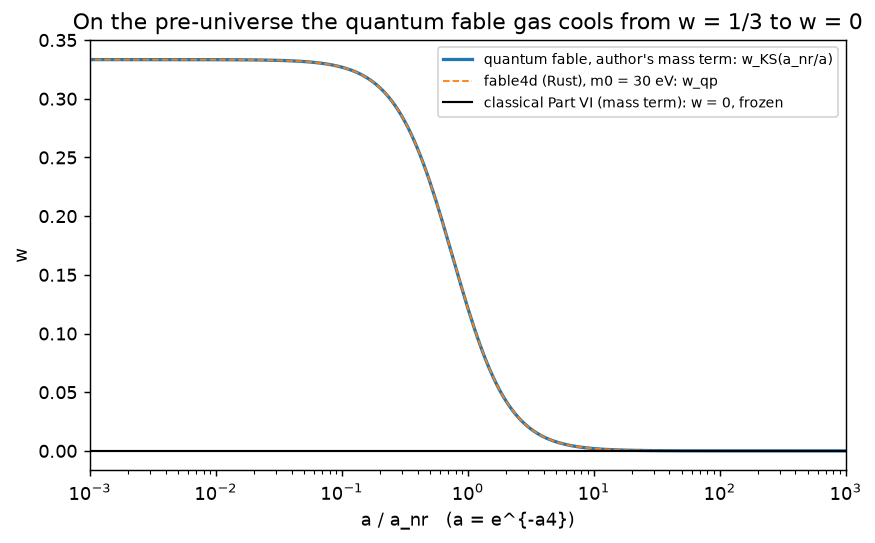
\includegraphics[width=0.75\linewidth]{nb05_preuniverse_cooling.png}
  \caption{\texttt{fable-cosmology/\allowbreak results/\allowbreak nb05\_preuniverse\_cooling.png} (notebook 05): the cooling on the
  pre-universe --- the quantum fable gas of the author's mass term goes from $w=1/3$ to $w=0$ as the observed
  sheet expands, while the classical Part~VI fable's $w=0$ is frozen (\secref{sec:4.1.6}).}
  \label{fig:nb05cool}
\end{figure}

\FloatBarrier

% ===============================================================================================
\subsection{The answers to [1] and [2]}
\label{sec:4.8}

The author asked: \textbf{[1]} ``Does this system provide a physical mechanism for a time-varying dark energy
equation of state (w)?'' \textbf{[2]} ``[\dots] time-varying dark matter equation of state (w)?'' The answers
below rest on the runs of \secref{sec:4.7} and the theorems of sections~\ref{sec:4.2}--\ref{sec:4.5}. Notebook 06
composes its own statement of the answers from its tables and asserts every qualitative claim in it; its
headlines read \cfnb{nb06 \S7}: ``\textbf{Formally yes, in the stabilized model, but in none of the runs is it
a viable one.}'' for [1], and ``\textbf{Yes, intrinsically, but for an allowed mass the variation is over long
before recombination.}'' for [2].

\subsubsection{Answer [1]: a time-varying dark-energy equation of state}
\label{sec:4.8.1}

\textbf{Yes, as a mechanism --- in the stabilized model, and only with a mass-varying potential. None of the
runs is a viable cosmology, and the mechanism carries every one of the following caveats.}

\paragraph{What the mechanism is.} In the Kohn--Sham ground state the fable's energy is
$\rho=\rho_{\mathrm{qp}}+\rho_U$, and the mean-field condensate $\rho_U=W(\sigma_7)-\sigma_7W'(\sigma_7)$ has
$P=-\rho_U$ along all seven spatial directions: a vacuum energy. When $W$ is not linear, $\rho_U$ changes as the
density falls, the quasiparticle mass $\meffx=W'(\sigma_7)$ changes with it, and the two parts exchange energy at
the rate $Q=\sigma_8\,dm/dt$ (\secref{sec:4.5.10}). The dark energy that an observer infers therefore varies in
time. For a massive power law $W=m_0\sigma+\lambda\sigma^\nu$ it is, in closed form and confirmed by the runs to
$1.2\times10^{-9}$,
\[
  \wDE(a)=-\frac{1-\nu}{1-\nu\,a^{-3(1-\nu)}},
\]
with a pole at $a=\nu^{1/(3(1-\nu))}$ ($0.5326$ for $\nu=0.236$) (\secref{sec:4.7.7}). The observer's CPL fits of
the eight dark-energy runs of \secref{sec:4.7.6} lie at distances from the supernova fit
$(w_0,w_a)=(-0.861,-0.60)$ of $7.43$ (\cfcode{power} $\nu=0.236$: $(-0.082,-7.986)$) to $11.2$ (\cfcode{expdamp}:
$(-0.128,-11.778)$) [file: \file{fable-cosmology/results/nb06_cpl_fits.csv}], and the fits are not faithful,
because $\wDE$ has a pole inside $0.3\leq a\leq1$ in all of them.

\paragraph{What does not give it.} With the author's mass term alone there is no dark energy at all: the fable
is a free gas that closes the budget, an Einstein--de Sitter-like universe with $\Omega_{f0}=0.95066$ and
$q_0=0.50005$ (\secref{sec:4.7.4}). With a mass term plus a bare $V_0$ (\cfcode{lambda-mass}), the observer infers
\textbf{exactly a cosmological constant}: CPL $(w_0,w_a)=(-1.000000,\,+1.3\times10^{-9})$,
$(-1.000000,\,+5.3\times10^{-11})$, $(-1.000000,\,+1.2\times10^{-13})$, $(-1.000000,\,+1.7\times10^{-14})$ at 30,
100, 1000, 2000\,eV --- no time variation (\secref{sec:4.7.5}). $V_0$ is a bare cosmological constant and is
reported as such.

\paragraph{The caveats, each quantified:}
\begin{enumerate}
  \item \textbf{No true phantom --- but an apparent phantom and phantom crossing in the observer's fit.} The
        fable's own equation of state never goes below $-1$: $\rho+\Pobs=\wF n/v\geq0$ is an identity
        (\secref{sec:4.5.9}), and the smallest $w_f$ over every run is \texttt{-0.9999987921}. The classical
        Part~VI crossing of $-1$ (at $V'(s^*)=0$, \secref{sec:3.1.12.7}) does \textbf{not} survive quantization.
        The \textbf{observer-inferred} dark energy, however, is phantom or crosses $-1$ inside $0.3\leq a\leq1$
        in 9 of 9 runs of \secref{sec:4.7.6} and in 90 of 90 scan points: subtracting cold dark matter with
        today's mass when the mass was different leaves
        $\rho_{\mathrm{DE}}+P_{\mathrm{DE}}\approx\bigl(\meffx(a)-\mtoday\bigr)\,n$, negative whenever $\meffx$
        grows (the mechanism of Das, Corasaniti and Khoury, Phys.\ Rev.\ D \textbf{73}, 083509 (2006)), with no
        phantom field. For the massive power law the crossing lies in the last output interval before today
        ($a>0.9727$), where the quasiparticles' kinetic energy, of relative size $\tfrac{3}{10}(\kF/m)^2$, finally
        exceeds $\bigl(\mtoday-\meffx(a)\bigr)\,n$ \cfnb{nb06 \S7}.
  \item \textbf{Mass-varying dark energy with massive dark matter needs a power law with $\nu<0.279$.} In the
        scans 28 of 90 points keep the fable massive over $10^{-3}\leq a\leq0.3$, all of them power laws; every
        \cfcode{quadratic} and \cfcode{expdamp} point is a massless gas (radiation) until late times and supplies
        no dark matter at recombination. A power law stays massive exactly when its bare mass $m_0$ is positive,
        i.e.\ when $\Omegaqp/U_t>\nu/(1-\nu)$; with the observed split $\Omegaqp=0.265$ that is $\nu<0.2788$
        (\secref{sec:4.7.8}). The massive mass-varying example with a larger quasiparticle share (Part~VIII's
        case: \cfcode{power}, $\nu=0.5$, $\mtoday=100$\,eV, $\Omegaqp=0.55$, no bare Lambda) has $\meffx$ rising
        from 27.15\,eV to 100.00\,eV, $w_f$ today $-0.4215$, $q_0=-0.1010$, and matter today
        $\Omegaqp+\Omega_{b0}=0.599$, about twice the measured $\Omega_m\approx0.315$ (Planck 2018): it is
        massive because its dark matter outweighs its dark energy, which the observed universe does not allow
        \cfnb{nb06 \S7}.
  \item \textbf{It is adiabatically unstable.} Every scan point that stays massive has $c_s^2<0$ after
        $a=10^{-3}$ (smallest $c_s^2$ between $-0.647$ and $-0.056$), and so do all 9 runs of \secref{sec:4.7.6}
        ($-0.611$ for $\nu=0.236$, $-0.364$ for Part~VIII's case, down to $-47.1$ for \cfcode{quadratic}). This is
        the adiabatic instability of mass-varying fermions (as found by Afshordi, Zaldarriaga and Kohri for
        mass-varying neutrinos).
  \item \textbf{The Dirac-sea vacuum energy demands a fine-tuning.} The renormalized sea energy that the no-sea
        functional drops changes, for a mass variation of order $m$, by $g\,m^4/(64\pi^2)$: $3.44$,
        $3.44\times10^{4}$, $3.44\times10^{8}$, $3.44\times10^{12}$ times $\rhoc$ at $m=0.01$, $0.1$, $1$, $10$\,eV,
        more than the critical density for $m>7.341$\,meV (\secref{sec:4.5.11}). Along every mass-varying run it
        changes by $\boldsymbol{1.31\times10^{13}}$ \textbf{to} $\boldsymbol{2.87\times10^{16}}$ \textbf{times the
        total density at $a\geq0.3$} (over the scans at least $3.79\times10^{9}$) \cfnb{nb06 \S7}. The runs read
        $W$ as the fully renormalized effective potential, which absorbs the sea energy only by fine-tuning the
        bare potential against it to that precision. The cosmological-constant problem is not solved.
  \item \textbf{It needs the stabilizer, which violates the null energy condition.} All of this holds with the
        hidden sheet held by $\Pstab=-F/2$ (today $-0.8428\,\rhoc$ in the $\Lambda$CDM-like runs, $-0.7003$ in
        Part~VIII's power case), a Lagrange multiplier, not a stress derived from any field, with zero energy
        density; it violates the null energy condition along $x_0$ on 100.0\,\% of the output rows of every
        stabilized run (\secref{sec:4.7.1}).
  \item \textbf{Without the stabilizer it is excluded (the \texttt{fable8d} no-go).} Left free, the hidden sheet
        is driven by dust and vacuum energy to the 7-dimensional isotropic attractor, and the observed Newton
        constant $G_4=G_8/\Vhidx$ varies: $G(a_i)/G(1)=$ $3.44\times10^{10}$, $1.85\times10^{17}$,
        $1.05\times10^{12}$, $1.07\times10^{12}$ in the four fable runs and $6.54\times10^{8}$ for radiation plus
        baryons alone; $\Delta G/G$ since nucleosynthesis is $-1$ (against about $0.1$), and $|d\ln G/dt|$ today
        $\geq2.31\times10^{-11}$\,/yr (against the lunar-laser-ranging bound $10^{-13}$\,/yr)
        (\secref{sec:4.7.10}). The only frozen-compatible Kohn--Sham fable is radiation (\secref{sec:4.5.7}).
  \item \textbf{The split into dark matter and dark energy is a convention.} The condensate $\rho_U$ is an
        8-dimensional vacuum energy, with $P=-\rho_U$ along the hidden directions as well; calling it dark
        energy and the quasiparticles dark matter is a choice of bookkeeping (\secref{sec:4.5.4}).
  \item \textbf{The approximations under which all of this holds:} semiclassical gravity
        ($G=\kappa\langle\That\rangle$); the Kohn--Sham mean field with exchange--correlation neglected
        (\secref{sec:4.5.12}); zero modes along $x_0$ and the hidden timelike sheet, with $x_0$ compactified (a
        Kaluza--Klein gap above the temperatures considered) and the hidden timelike sheet a formal comoving
        volume (compactifying it gives closed timelike curves); the asymptotic Bianchi-I reading of the
        primordial field, which neglects terms of order $\cot(6Hx_0)$ and $\cot^2(6Hx_0)$ (\secref{sec:4.3.3});
        $g_*(T)$ not followed.
\end{enumerate}

\subsubsection{Answer [2]: a time-varying dark-matter equation of state}
\label{sec:4.8.2}

\textbf{Yes, intrinsically: the quantized fable's dark-matter equation of state runs from $1/3$ to 0. For an
allowed mass the variation is over long before recombination.}
\begin{enumerate}
  \item \textbf{The mechanism.} The fable's quasiparticles are a degenerate Fermi gas ($g=8$ states per
        momentum), and their equation of state is $\wDM=\PKS/\epsKS$, a function of $x=\kF/|m|$ alone that rises
        monotonically from 0 (dust) to $1/3$ (radiation) (\secref{sec:4.1.6}). As the universe expands,
        $\kF=k_{F0}/a$ falls, and $\wDM$ falls from $1/3$ to 0: \textbf{a time-varying dark-matter equation of
        state}, which is a property of the quantum gas and has no counterpart in the classical Part~VI fable
        (whose $w$ was frozen on the pre-universe and 0 for the mass term). Every run starts at
        $\wDM=0.333333$ and ends today at most $8.1\times10^{-8}$ \cfnb{nb06 \S7}; the transition is at
        $\anr=k_{F0}/m$, $4.466\times10^{-6}$ for 30\,eV and $4.163\times10^{-8}$ for 1\,keV, scaling as
        $m^{-4/3}$ (sections~\ref{sec:4.7.4}--\ref{sec:4.7.5}). The same cooling happens on the pre-universe itself,
        on the canonical frame with $a_4$ free, whenever the observed sheet expands ($a_4'<0$, \secref{sec:4.1.6}).
  \item \textbf{How heavy it must be, and hence when the variation happens.} A fable that is all of the dark
        matter is radiation before $\anr$: $\DNeff(\mathrm{BBN})=6.692\,(m/\mathrm{eV})^{-4/3}<0.3$ requires
        $m>10.3$\,eV ($<0.2$: $m>13.9$\,eV). Free streaming is far more restrictive: matching the rms velocity of
        the Lyman-alpha-allowed thermal warm dark matter requires $m\approx1125$--$1807$\,eV
        (${\sim}1.1$--$1.8$\,keV, a velocity-matching estimate, not a transfer-function computation), and the
        Tremaine--Gunn phase-space bound for illustrative dwarf spheroidals gives $m>231$--$358$\,eV
        (\secref{sec:4.7.9}). At such masses the change of $\wDM$ from $1/3$ to 0 happens around
        $\anr=4.16\times10^{-8}$ (1\,keV) or $1.65\times10^{-8}$ (2\,keV): \textbf{indistinguishable from cold dark
        matter in the late universe}.
  \item \textbf{With a mass-varying potential the effective equation of state varies late.} The quasiparticles
        then exchange energy with the condensate ($Q=\sigma_8\,dm/dt$), and their effective equation of state
        $\wDMeff=\wDM-\sigKS\,(dm/dN)/(3\epsKS)$ ranges, after $a=10^{-3}$, over $[-0.611,\,+9.85\times10^{-5}]$
        (\cfcode{power} $\nu=0.236$, 30\,eV), $[-0.611,\,+3.59\times10^{-6}]$ (100\,eV), $[-27.6,\,+0.333]$ and
        $[-27.7,\,+0.333]$ (\cfcode{power} $\nu=0.5$), $[-21.8,\,+0.333]$ (\cfcode{expdamp}), $[-47.1,\,+0.333]$
        (\cfcode{quadratic}), and $[-0.364,\,-3.89\times10^{-5}]$ (Part~VIII's case) (\secref{sec:4.7.6}). This late
        variation is the same exchange that makes the inferred dark energy vary in [1], and it carries all of
        [1]'s caveats (adiabatic instability, the sea energy, the viability window $\nu<0.2788$).
  \item \textbf{The author's mass term alone is dark matter without dark energy.} $W=m_0\sigma$ gives an
        Einstein--de Sitter-like universe ($q_0=+0.50005$, age 9.67\,Gyr with $H_0=67.4$\,km/s/Mpc), not ours;
        with a bare cosmological constant (\cfcode{lambda-mass}) it is $\Lambda$CDM with fable dark matter
        ($q_0=-0.52845$, age 13.8000\,Gyr) (sections~\ref{sec:4.7.4}--\ref{sec:4.7.5}).
  \item \textbf{The same caveats as [1]} apply: the stabilized model with its NEC-violating stabilizer (without
        it the Newton constant varies by $6.5\times10^{8}$ to $1.9\times10^{17}$); the split into dark matter and
        dark energy is a convention; semiclassical gravity, the Kohn--Sham mean field with $E_{\mathrm{xc}}$
        neglected (exact for the author's mass term, which is free), zero modes along the hidden directions,
        the asymptotic reading of the primordial field.
\end{enumerate}

% ===============================================================================================
\needspace{6\baselineskip}
\section{The design review: four lenses, four skeptics, every finding, and every correction}
\label{sec:5}

Nothing of Efforts A and B was implemented before its design had been attacked. This section records the attack: how it was organized, every finding with its severity and its verdict, what was adopted, the sub-claims of the reviewers that the skeptics refuted, the points the skeptics found that the reviewers had missed, and the corrections that were found only later, by the implementation and the checks. Each adopted correction is named with the section of this page where its content now stands.

\needspace{6\baselineskip}
\subsection{How the review was organized}
\label{sec:5.1}

\needspace{8\baselineskip}
\textbf{The design (revision 1)}, written on 2026-09-24 before any code, fixed the conventions of the notebook (never to be changed), recorded six facts already computed by probes (F1 the Clifford symmetry table; F2 the Grassmann consequences; F3 the Einstein tensor of the canonical metric, which is not a vacuum solution; F4 the generalized warped frame and its (0,4) equation; F5 the 8-dimensional Bianchi-I system; F6 the quantization algebra: $G = -i \sigma_{16} \gamma^{4}$, signature (8,8), $J$, the plane-wave spectrum), stated the physics of Efforts A (A.1 refinement, A.2 Lagrangian, A.3 field equations, A.4 quantization, A.5 EMT, A.6 expectation values, A.7 spin connection) and B (B.1--B.6: the semiclassical system, the canonical ansatz, the present-universe models, the DFT states, the spin connection of the dynamical frames, the answers), gave the implementation plan, and asked the reviewers eight questions to try to break:

{\small
\begin{longtable}{@{}p{0.058\linewidth}p{0.882\linewidth}@{}}
\toprule
\raggedright  & \raggedright question \tabularnewline
\midrule
\endhead
\raggedright Q1 & \raggedright Is the Dirac-bracket anticommutator (factor, sign, $H/\sqrt{g}$, $-i \sigma_{16} \gamma^{4}$) right, including for the symmetrized Lagrangian and on the curved slice? \tabularnewline
\raggedright Q2 & \raggedright Is the Krein/$J$ quantization legitimate (Hermiticity of the interacting $H$ under the $J$-involution; what exactly is lost; does $J$ commute with every term of the admissible-sector Hamiltonian, the spin connection included)? \tabularnewline
\raggedright Q3 & \raggedright Is the impossibility of a Majorana mass / scalar bilinear right for every candidate bilinear, and is ``fermion fable must be complex'' stated with the right scope? \tabularnewline
\raggedright Q4 & \raggedright The EMT operator: sign and normalization against Part VI; symmetrization; the spin-connection-variation argument; conservation with independent $\Psi$, $\bar\Psi$. \tabularnewline
\raggedright Q5 & \raggedright Kohn--Sham thermodynamics: the closed forms, $g = 8$, the classical limit, the no-sea statement, the mass-term conclusions. \tabularnewline
\raggedright Q6 & \raggedright The 8D Einstein equations: F3--F5, the frozen-hidden theorem and its corollary, the conservation law, the units ($\kappa_8$ against $\kappa_4$), the Bianchi-I claim, the negative background energy. \tabularnewline
\raggedright Q7 & \raggedright DFT: the functional $E_{n}[\sigma]$ on $(-n, n)$, uniqueness, the $\Delta$SCF / wall-state construction, the MIT condition in this real-Clifford convention, whether the wall problem is well posed and bound states exist, whether \cftt{expdamp} pins $\sigma \leq s_1$. \tabularnewline
\raggedright Q8 & \raggedright Cosmology: are the runs meaningful ($\Omega$ values, time interval, shooting), the definitions of $w_{\mathrm{DE,eff}}$ and $w_{\mathrm{DM}}$, adiabatic instability, the bounds on $G$; are answers [1] and [2] honest? \tabularnewline
\bottomrule
\end{longtable}
}

\needspace{8\baselineskip}
\textbf{The four lenses.} Each reviewer ran its own probes on the notebook's own state (the Input cells loaded headlessly, or the notebook's $T_{16}$ and $\sigma_{16}$ exported to Python) and wrote findings, each with an ID, a severity (critical, major, minor), a kind (wrong, incomplete, ill-posed, hidden assumption, implementation risk, better formulation), the statement and a proposed fix:

{\small
\begin{longtable}{@{}p{0.486\linewidth}p{0.339\linewidth}p{0.096\linewidth}@{}}
\toprule
\raggedright lens & \raggedright covers & \raggedright findings \tabularnewline
\midrule
\endhead
\raggedright quantization: canonical quantization in 4+4 signature, Grassmann and Majorana algebra, Krein spaces & \raggedright F1, F2, F6; A.1, A.2, A.4; Q1--Q3 & \raggedright \cftt{QK-{}1} \dots{} \cftt{QK-{}11} \tabularnewline
\raggedright field equations, energy--momentum tensor operator, canonical spin connection & \raggedright A.2, A.3, A.5, A.7, B.5; Q4 & \raggedright \cftt{EMT-{}1} \dots{} \cftt{EMT-{}11} \tabularnewline
\raggedright the 8D Einstein equations with fable as source, and the cosmological runs & \raggedright F3, F4, F5; B.1, B.2, B.3, B.6; Q6, Q8 & \raggedright \cftt{E1} \dots{} \cftt{E12} \tabularnewline
\raggedright density-functional theory and the numerics & \raggedright A.6, B.3 sources, B.4; Q5, Q7; the Rust and Python plan & \raggedright \cftt{DFT-{}1} \dots{} \cftt{DFT-{}16} \tabularnewline
\bottomrule
\end{longtable}
}

\textbf{The four skeptics.} Each lens was followed by an independent skeptic, who received the findings and tried to \textbf{refute} each one with computations of its own (its own Riemann-tensor and spin-connection code, its own Python on the exported matrices, its own numerical runs), and returned a verdict per finding --- \emph{confirmed}, \emph{partly confirmed} or \emph{refuted} --- with a corrected fix wherever it disagreed, and a list of what the reviewer had \textbf{missed}.

\textbf{The outcome.} 50 findings: \textbf{30 confirmed, 20 partly confirmed, 0 refuted.} Where a finding was only partly confirmed, the skeptic's corrected fix was adopted. All adopted corrections were written into an addendum to the design (revision 2), which overrides revision 1 wherever they differ, and then implemented. The DFT skeptic's final verdicts came last and override the addendum where they differ.

{\footnotesize
\setlength{\tabcolsep}{3pt}
\begin{longtable}{@{}p{0.345\linewidth}p{0.233\linewidth}p{0.263\linewidth}p{0.059\linewidth}@{}}
\toprule
\raggedright lens & \raggedright confirmed & \raggedright partly confirmed & \raggedright refuted \tabularnewline
\midrule
\endhead
\raggedright quantization (\cftt{QK}) & \raggedright 3 (\cftt{QK-{}2}, \cftt{QK-{}7}, \cftt{QK-{}8}) & \raggedright 8 (\cftt{QK-{}1}, \cftt{3}, \cftt{4}, \cftt{5}, \cftt{6}, \cftt{9}, \cftt{10}, \cftt{11}) & \raggedright 0 \tabularnewline
\raggedright field equations / EMT / spin connection (\cftt{EMT}) & \raggedright 9 (\cftt{EMT-{}1}, \cftt{3}--\cftt{10}) & \raggedright 2 (\cftt{EMT-{}2}, \cftt{EMT-{}11}) & \raggedright 0 \tabularnewline
\raggedright Einstein / cosmology (\cftt{E}) & \raggedright 6 (\cftt{E2}, \cftt{E4}, \cftt{E6}, \cftt{E8}, \cftt{E10}, \cftt{E11}) & \raggedright 6 (\cftt{E1}, \cftt{E3}, \cftt{E5}, \cftt{E7}, \cftt{E9}, \cftt{E12}) & \raggedright 0 \tabularnewline
\raggedright DFT / numerics (\cftt{DFT}) & \raggedright 12 (\cftt{DFT-{}1}--\cftt{3}, \cftt{5}, \cftt{9}--\cftt{16}) & \raggedright 4 (\cftt{DFT-{}4}, \cftt{6}, \cftt{7}, \cftt{8}) & \raggedright 0 \tabularnewline
\bottomrule
\end{longtable}
}

\needspace{10\baselineskip}
\subsection{The quantization lens (\texorpdfstring{\cftt{QK}}{QK})}
\label{sec:5.2}

{\footnotesize
\setlength{\tabcolsep}{3pt}
\begin{longtable}{@{}p{0.055\linewidth}p{0.095\linewidth}p{0.270\linewidth}p{0.310\linewidth}p{0.200\linewidth}@{}}
\toprule
\raggedright ID & \raggedright severity, kind & \raggedright the finding & \raggedright verdict and the skeptic's correction & \raggedright adopted, and where it stands now \tabularnewline
\midrule
\endhead
\raggedright QK-1 & \raggedright major, wrong & \raggedright The admissibility argument had the wrong mechanism: the free theory below threshold can be quantized with a momentum-dependent $J_k$; the real obstruction is \textbf{locality} --- one momentum-independent $J'$ must commute with $\beta = -i T_{16}[4]$ and every one-particle generator $E_k = G h_k$; no positive $J'$ exists once a hidden momentum is present; at threshold $E_k$ is nilpotent (Jordan blocks); above it the modes are $G$-neutral. & \raggedright \textbf{Partly confirmed.} Computed with the notebook's matrices: the boosted $J' = S^{-1} J S$ works for one mixed momentum ($[J', E] = 10^{-15}$, $GJ'$ positive, minimum eigenvalue 0.655); the theorem is about the \textbf{span} $V$ of the mode momenta: positive quantization iff $V$ is spacelike-definite; $J'$ unique (with $J'^{2} = 1$) when $V=\operatorname{span}(x_0..x_3)$. The reviewer's above-threshold frequencies $\pm 1.705872 i$ were wrong: for $k=(0,.75,1,0\,|\,k_5=2)$, $m = 1$ they are $\pm 1.19896 i$. Below threshold the free field is quantizable mode by mode but not uniformly: $\operatorname{cond}(G J_k) = (m + k_5)/(m - k_5)$ = 3, 19, 199, 1999 at $k_5 = .5, .9, .99, .999$. & \raggedright The theorem as corrected, with its proof ingredients as assertions ($[E_k, \beta] = 2 i T_{k}$, the $T_{5}$ anti-congruence, the traceless certificate, the positive boosted $J'$, the rank-8 Jordan block with $E^{2} = 0$): section~\ref{sec:3.5.10} (\cftt{ADMISSIBILITY}). \tabularnewline
\raggedright QK-2 & \raggedright major, ill-posed & \raggedright ``Physical states obey $P_{5} = P_{6} = P_{7} = 0$'' is not a superselection rule: pairs $(k_h, -k_h)$ have $P_h = 0$, and $V(s)$ contains $b^\dagger_{k_h}b^\dagger_{-k_h}b_0b_0$; the admissible theory is a \textbf{truncation} needing a finite hidden volume. & \raggedright \textbf{Confirmed} (derivation; normalization by projection gives $(H/(V_{\mathrm{hid}} \sqrt{g})) G \delta^{4}$). $V_{\mathrm{hid}}$ is a coordinate volume; the truncated theory is a (4,1)-dimensional theory whose Cauchy surface is $x_0..x_3$. & \raggedright The truncation $\Psi=\Psi(x_0..x_4)$ with finite $V_{\mathrm{hid}}$ (closed timelike curves stated); the anticommutator $(H/(V_{\mathrm{hid}} \sqrt{|g|})) G \delta^{4}$; the Tomonaga--Schwinger remark kept only as $[P_4, P_h] = 0$: sections~\ref{sec:3.5.1}, \ref{sec:3.5.4}. \tabularnewline
\raggedright QK-3 & \raggedright major, incomplete & \raggedright Under the $J$-involution, $\Psi^{\ddagger} M \Psi$ is Hermitian iff $[J, M] = 0$ and anti-Hermitian iff $\{J, M\} = 0$; $\hat T_{\mu h}$, $\hat T_{hh'}$ and $j^{h}$ are anti-Hermitian. & \raggedright \textbf{Partly confirmed. Refuted sub-claim:} $\hat T_{hh'}$ ($h \neq h'$) is \textbf{not} anti-Hermitian --- its connection pieces commute with $J$, and for $x_5..x_7$-independent $\Psi$ it vanishes identically on all three frames. The mixed $\hat T_{\mu h}$ are nonzero and anti-Hermitian; an anti-Hermitian operator has a purely imaginary expectation in every state, so $G_{\mu h}=\kappa\langle\hat T_{\mu h}\rangle$ is consistent only where the expectation is 0, which hidden-SO(3) invariance ensures. & \raggedright The Hermiticity table with $\hat T_{hh'}\equiv0$, $\hat T_{hh}=g_{hh}\hat L$, anti-Hermitian $\hat T_{\mu h}$ and $j^{h}$ with zero expectation in hidden-SO(3)-invariant states: sections~\ref{sec:3.5.8}, \ref{sec:3.6.5}. \tabularnewline
\raggedright QK-4 & \raggedright major, implementation risk & \raggedright Part V/VI's ``$\hat L$ with $D$ = $\hat L$ with $\partial$'' holds only for real commuting $\Psi$; for Grassmann fields the unsymmetrized connection term $-3H\cot^2\,\Psi^\ddagger\sigma_{16}T_{16}[0]\Psi$ is nonzero and anti-Hermitian, and the unsymmetrized partial-derivative Lagrangian gives inconsistent equations. & \raggedright \textbf{Partly confirmed. Overstated part:} ``never assert covariant = partial'' is too strong --- for the \textbf{symmetrized} Lagrangian $\hat L_{\mathrm{sym}}(D)-\hat L_{\mathrm{sym}}(\partial)=\frac{1}{2H}\,\bar\Psi\sum_\mu\{\gamma^\mu,\Gamma_\mu\}\Psi$, which is identically 0 on the canonical, warped and Bianchi-I frames, so the identity holds there in symmetrized form. F2(a) (no dynamics for a real Grassmann field) holds on \textbf{every} frame. & \raggedright Only the symmetrized Lagrangian; the four facts (a)--(f) as assertions: section~\ref{sec:3.3} (\cftt{LAGRANGIAN (a)--(f)}), 3.2.3. \tabularnewline
\raggedright QK-5 & \raggedright major, better formulation & \raggedright $J$ has concrete content: $\sigma_{16} = J \beta$, $J = -i \Omega T_{16}[0]$; with $\Psi^\dagger:=\Psi^\ddagger J$ the author's conjugate is the observer's Dirac adjoint; fable is four 4D Dirac flavours with a flavour metric of signature (2,2) replaced by 1; legitimate for fermions, not for bosons. & \raggedright \textbf{Partly confirmed.} Not verified: ``J gives reflection positivity'' --- dropped. The bosonic mechanism is not ``a ghost'': for a commuting field $H$ has 8 negative-frequency modes per $k$ and is unbounded below; making it bounded below turns 4 modes into negative-norm modes. The $J$ *-structure differs from the classical reality structure on $J$-odd observables, so the classical theory is the limit of the $J$-even sector only. \textbf{Missed point:} the prescription $b_u^\dagger:=\eta_u\,b_u^\ddagger$ is basis-dependent (a Krein boost inside a (4,4) eigenspace gives $\|J_k-J\|=4.45$ and a non-Hermitian $s$); the adjoint must be $\Psi^{\ddagger} J$, mode-independent. & \raggedright Sections~\ref{sec:3.5.5}, \ref{sec:3.5.6}, \ref{sec:3.5.13} ($J$, \cftt{KREIN MODES [control]}); two symbols for the classical conjugation and the Hilbert adjoint. \tabularnewline
\raggedright QK-6 & \raggedright minor, wrong & \raggedright The symmetry count: the group commuting with $J$ is Spin(4,1)$\times$Spin(3) (13 generators); the 15 lost are 12 boosts and 3 \textbf{rotations} (the design had called them boosts); chirality $T_{16}[8]$ is lost; $p = \bar\Psi T_{16}[8] \Psi$ is anti-Hermitian; $G$ is Spin(4,3)-invariant (21). & \raggedright \textbf{Partly confirmed. Misleading sub-claim:} the chirality subspaces \textbf{are} orthogonal in the Hilbert product ($T_{16}[8]$ is Hermitian); what is true is that $J$ is chirality-odd, so each chirality subspace is $G$-null and the $J$-vacuum is not chirality-graded. $ip$ is $J$-Hermitian but classically imaginary, so $V$ depends on $s$ only. & \raggedright Section~\ref{sec:3.5.9}, \ref{sec:3.5.7}. \tabularnewline
\raggedright QK-7 & \raggedright minor, incomplete & \raggedright The four candidate matrices are only two ($C_+ T_{8} = \sigma_{16}$); the invariant forms are $\operatorname{span}\{\sigma_{16}, \sigma_{16} T_{8}\}$, both symmetric and chirality-diagonal; Majorana has one quartic scalar and a non-dynamical commuting shadow; complex Weyl spinors do not propagate either; the complex spinor has two scalar bilinears and 6 quartic invariants. & \raggedright \textbf{Confirmed} (full rank table \cftt{S|\allowbreak{}S,\allowbreak{} A|\allowbreak{}S,\allowbreak{} A|\allowbreak{}A,\allowbreak{} S|\allowbreak{}A,\allowbreak{} S|\allowbreak{}S,\allowbreak{} A|\allowbreak{}S,\allowbreak{} A|\allowbreak{}A,\allowbreak{} S|\allowbreak{}A,\allowbreak{} S|\allowbreak{}S} for ranks 0--8; invariant forms of dimension 2; 0 singlets in $\Lambda^{2}(16)$). & \raggedright ``The minimal, not the unique, field'': sections~\ref{sec:3.2.1}--\ref{sec:3.2.8} (\cftt{REFINEMENT (a)}, \cftt{(b)}). \tabularnewline
\raggedright QK-8 & \raggedright minor, hidden assumption & \raggedright When $\sqrt{g}$ depends on $x_{4}$, $\Psi$ is not a canonical Heisenberg field; quantize $\chi = (\sqrt{|g|}/H)^{1/2} \Psi$. & \raggedright \textbf{Confirmed.} & \raggedright Section~\ref{sec:3.5.16}; on the dynamical frames, section~\ref{sec:4.4.6}. \tabularnewline
\raggedright QK-9 & \raggedright minor, hidden assumption & \raggedright Hermiticity needs a $J$-compatible boundary condition in $x_{0}$: the bag condition $T_{16}[0] \Psi = \pm \Psi$. & \raggedright \textbf{Partly confirmed. Overstated:} ``vanishes at both ends'' --- the wall is at finite proper distance ($z\approx3Hx_0^2$), the operator is \textbf{regular} there and needs a condition; at $z \to \infty$ it is limit-point and none can be imposed. & \raggedright One-particle space $L^2(dz)$; the condition at the wall only: section~\ref{sec:3.5.12}. \tabularnewline
\raggedright QK-10 & \raggedright minor, wrong & \raggedright $j^{\mu} = i \bar\Psi \gamma^{\mu} \Psi$ has the wrong sign and normalization to be the number current. & \raggedright \textbf{Partly confirmed:} the calculation is right, ``wrong'' is overstated --- $j^{\mu}$ is a legitimate conserved current that needs its normalization stated. & \raggedright $n^\mu:=-(i/H)\,\bar\Psi\gamma^\mu\Psi$, $n^{4} = \Psi^{\dagger} \Psi/H \geq 0$; a positive-frequency $J$-mode carries $j$-charge \ensuremath{-}1: section~\ref{sec:3.4.10}. \tabularnewline
\raggedright QK-11 & \raggedright minor, better formulation & \raggedright $V(s)$ needs no Weyl ordering in the Hamiltonian (spectral calculus of one Hermitian operator); the ordering appears only in the Heisenberg equation, as an insertion average. & \raggedright \textbf{Partly confirmed:} the design's Weyl-symmetrized product is already identical to the insertion average (Fock check to $1.1\times10^{-16}$); the real addition is that $V({:}s{:})$ needs no ordering. & \raggedright Section~\ref{sec:3.4.9}. \tabularnewline
\bottomrule
\end{longtable}
}

What the quantization lens confirmed as right (11 items): the full Clifford symmetry table; the invariant forms; $G = -i \sigma_{16} \gamma^{4} = J$ Hermitian with $J^{2} = 1$ and signature (8,8); the eightfold $\pm \omega$ modes for admissible momenta; $\omega^{2} = k_s^{2} - k_h^{2} + m^{2}$; the $J$ commutation relations; $\Gamma_{\mu}$ real with $\sigma_{16} \Gamma_{\mu}$ antisymmetric; the real commuting shadow equals Part VI's \cftt{cfLhatFable}; the commutant $M_4(\mathbb{C})$ (four flavours); the Hermiticity of $H_{\mathrm{free}} + \lambda s^{2}$; the rescaling $\sqrt{|g|}=\sec(6Hx_0)$.

\needspace{10\baselineskip}
\subsection{The field-equation, energy--momentum-tensor and spin-connection lens (\texorpdfstring{\cftt{EMT}}{EMT})}
\label{sec:5.3}

{\footnotesize
\setlength{\tabcolsep}{3pt}
\begin{longtable}{@{}p{0.055\linewidth}p{0.095\linewidth}p{0.270\linewidth}p{0.310\linewidth}p{0.200\linewidth}@{}}
\toprule
\raggedright ID & \raggedright severity, kind & \raggedright the finding & \raggedright verdict and the skeptic's correction & \raggedright adopted, and where it stands now \tabularnewline
\midrule
\endhead
\raggedright EMT-1 & \raggedright major, implementation risk & \raggedright The design gave the wrong reason for the covariant derivative in $T_{\mu\nu}$: varying a partial-derivative Lagrangian gives $T_{\mathrm{par}}$, not conserved, differing from $T_{\mathrm{cov}}$ in 21 off-diagonal components; the spin-connection variation is \textbf{identically zero} ($\delta\omega_{[cab]}=0$ for symmetric tetrad variations). & \raggedright \textbf{Confirmed} (own first-order symmetric tetrad perturbation, all 36 functions generic). Addition: on the canonical frame $T_{\mathrm{cov}} = T_{\mathrm{par}}$ on the diagonal \textbf{and} on $(0,4)$; $(5,6)$ vanishes identically; the control needs a non-vacuous pair such as $(1,4)$, $(0,1)$, $(1,5)$, $(5,4)$, $(0,5)$. Do not run the symbolic divergence of $T_{\mathrm{par}}$ (it ran more than 9 minutes). & \raggedright Hilbert = $T_{\mathrm{cov}}$ off shell, the variation piece zero, Hilbert $\neq$ $T_{\mathrm{par}}$ at a non-vacuous pair: sections~\ref{sec:3.6.1}, \ref{sec:3.8.12.5} (\cftt{EMT}). \tabularnewline
\raggedright EMT-2 & \raggedright major, wrong & \raggedright ``The connection commutes with $J$'' holds only for $\gamma^{\mu} \Gamma_{\mu}$ and $\Gamma_0..\Gamma_4$; $\Gamma_{5}, \Gamma_{6}, \Gamma_{7}$ \textbf{anticommute} with $J$. & \raggedright \textbf{Partly confirmed. Part of the finding wrong:} in any Hamiltonian $\Gamma_{h}$ enters only as $\sigma_{16} \gamma^{h} \Gamma_{h}$, and $[J, \gamma^{h} \Gamma_{h}] = 0$ for \textbf{each} $h$ separately; the $J$-odd objects are the bare $\Gamma_{h}$ in $T_{\mathrm{cov}}$ $(0,h)$, $(i,h)$, $(4,h)$ and the hidden momenta. The expectation argument is right and needs $J$-eigenmodes. & \raggedright The full $J$ table, per $\mu$: sections~\ref{sec:3.5.8}, \ref{sec:3.8.12.6}, \ref{sec:4.4.7} (\cftt{J TABLE}). \tabularnewline
\raggedright EMT-3 & \raggedright minor, wrong & \raggedright ``On shell $\hat L=sV'-V$ (bilinear part vanishes)'' is false: the kinetic bilinear equals $s V'(s)$. & \raggedright \textbf{Confirmed.} & \raggedright Section~\ref{sec:3.6.4}. \tabularnewline
\raggedright EMT-4 & \raggedright minor, incomplete & \raggedright The on-shell components were missing: trace $7sV'-8V$; $\rho = V + K_h$; $T^i{}_i=T^h{}_h=sV'-V$; $T^0{}_0=sV'-V+K_h$; $K_h$ symmetrized, 0 on the rescaled $x_{4}$-only solutions. & \raggedright \textbf{Confirmed.} Caveats added: calling $T^h{}_h$ a pressure along the hidden \textbf{timelike} directions is a naming convention; $K_h = 0$ holds on the $x_{4}$-only family, which solves the equation only if $V'' s' = 0$. & \raggedright Section~\ref{sec:3.6.4} (\cftt{EMT ON SHELL}). \tabularnewline
\raggedright EMT-5 & \raggedright minor, hidden assumption & \raggedright Part VI's drop-out mechanism does not carry over to complex fields; in the symmetrized Lagrangian the connection drops iff the \textbf{matrix} $\{\gamma^\mu,\Gamma_\mu\}=\tfrac12\,\omega_{[cab]}\,\gamma^{cab}$ vanishes. & \raggedright \textbf{Confirmed.} & \raggedright Sections~\ref{sec:3.3.3}, \ref{sec:3.8.12.2}. \tabularnewline
\raggedright EMT-6 & \raggedright minor, better formulation & \raggedright With the symmetrized Lagrangian the Hamiltonian density contains \textbf{no} connection; it re-emerges in the equation of motion as $\gamma^{\mu} \Gamma_{\mu} = (1/2)(1/\sqrt{g}) \partial_\mu(\sqrt{g} \gamma^{\mu})$. & \raggedright \textbf{Confirmed.} Addition: the unsymmetrized and symmetrized integrated Hamiltonians differ only by the surface term $(1/2H)\bigl[\csc(6Hx_0)\,\bar\Psi T_{16}[0]\Psi\bigr]$ at the wall, which vanishes exactly when the wall condition kills the normal current. & \raggedright Sections~\ref{sec:3.5.11}, \ref{sec:3.8.12.4}. \tabularnewline
\raggedright EMT-7 & \raggedright minor, incomplete & \raggedright On the dynamical frames $\Gamma_{0} \neq 0$ when $C' \neq 0$; the complete non-zero $\omega$ lists must be asserted. & \raggedright \textbf{Confirmed} (own routine reproduces \cftt{GammaSpinCanonical}; the warped and Bianchi-I lists; $\Gamma_{4} = 0$). & \raggedright Section~\ref{sec:4.4.2} (the complete lists). \tabularnewline
\raggedright EMT-8 & \raggedright minor, hidden assumption & \raggedright The commuting-placeholder conservation proof holds for Grassmann fields only because the on-shell divergence is linear in $\bar\Psi$-left bilinears with coefficients that are functions of the \textbf{even} composites $s$ and $ds$. & \raggedright \textbf{Confirmed} (derivation checked step by step). & \raggedright Section~\ref{sec:3.6.3}. \tabularnewline
\raggedright EMT-9 & \raggedright minor, better formulation & \raggedright The exact 8+8 form with its conjugate rows; $s$ is chirality-diagonal, so the axial phase leaves $V(s)$ invariant but \textbf{not} the kinetic term: the only U(1) is the vector one. & \raggedright \textbf{Confirmed} (the internal-symmetry Lie algebra is 1-dimensional). & \raggedright Sections~\ref{sec:3.4.3}, \ref{sec:3.4.6}, \ref{sec:3.4.11} (\cftt{SYMMETRY}). \tabularnewline
\raggedright EMT-10 & \raggedright minor, better formulation & \raggedright The rescaling theorem in frame-independent form: $\gamma^{\mu} \Gamma_{\mu} = -(1/2) T_\mu \gamma^{\mu}$, $T_\mu$ the Weitzenböck torsion vector; on the warped frame $\Psi=\sqrt{\sin}\,(A^3B^3C)^{-1/2}\chi$ and $\{\chi,\chi^\dagger\}=H\cot(6Hx_0)\,G\,\delta^7$, independent of $x_{4}$. & \raggedright \textbf{Confirmed.} Wording: the $\chi$ anticommutator is $x_{4}$-independent and the dilution is carried by the prefactor; the $\chi$ dynamics stay time-dependent through the frame. & \raggedright Sections~\ref{sec:3.8.12.3}, \ref{sec:4.4.5}, \ref{sec:4.4.6}. \tabularnewline
\raggedright EMT-11 & \raggedright minor, hidden assumption & \raggedright For nonlinear $V$ the operator equation is $\gamma^\mu D_\mu\Psi=H\,{:}V'(s)\Psi{:}$, differing from the naive product by Hartree/Fock contractions. & \raggedright \textbf{Partly confirmed. Imprecise:} the contraction terms are not all c-number multiples of $\Psi$; the J-vacuum sea matrix has a scalar part (divergent, renormalizes $V'$) and a $\gamma^{4}$ part (the sea charge, a constant chemical-potential shift, removed by charge-symmetric ordering or a phase, \textbf{not} by renormalizing $V$). & \raggedright Section~\ref{sec:3.4.9}. \tabularnewline
\bottomrule
\end{longtable}
}

What the skeptic of this lens found \textbf{missed}: the $x_{4}$-only family $\Psi=\sqrt{\sin}\,\Psi'(x_4)$ solves the field equation only if $V'' s' = 0$ (for the complex field $s'$ is conserved, so null data $s' = 0$ give $x_{4}$-only solutions for \textbf{any} $V$, with $\rho = V(0)$) --- section~\ref{sec:3.4.8}; normal ordering on an $x_{4}$-dependent background is ambiguous, and ``$\langle{:}T{:}\rangle=0$ in the vacuum'' holds only for static backgrounds or adiabatically --- section~\ref{sec:3.7.3}; the witness pairs for $T_{\mathrm{cov}}$ against $T_{\mathrm{par}}$ are frame-specific; and the per-$\mu$ identity $\{\gamma^{\mu}, \Gamma_{\mu}\} = 0$ (not only the sum) is what gives the individual pressures --- section~\ref{sec:3.6.4}.

\needspace{10\baselineskip}
\subsection{The Einstein and cosmology lens (\texorpdfstring{\cftt{E}}{E})}
\label{sec:5.4}

{\footnotesize
\setlength{\tabcolsep}{3pt}
\begin{longtable}{@{}p{0.055\linewidth}p{0.095\linewidth}p{0.270\linewidth}p{0.310\linewidth}p{0.200\linewidth}@{}}
\toprule
\raggedright ID & \raggedright severity, kind & \raggedright the finding & \raggedright verdict and the skeptic's correction & \raggedright adopted, and where it stands now \tabularnewline
\midrule
\endhead
\raggedright E1 & \raggedright major, wrong & \raggedright $W = m_0 \sigma + (\lambda/2) \sigma^{2}$ is \textbf{not} frozen-hidden-compatible; the condition holds only for $W = c \sigma^{2}$, and then the gap is nonzero only while $\lambda g k_F^{2}/(4 \pi^{2} v) > 1$. The reviewer wrote the driver as $F = \sigma W' - 2W$. & \raggedright \textbf{Partly confirmed. Sign corrected:} at self-consistency $F = \rho - 3P_{\mathrm{obs}} + 2P_{\mathrm{hid}} = 2W - \sigma W'$ (the reviewer's own number, $F = +m_0 \sigma$, agrees with this sign); with $V_0$, $F=2V_0+m_0\sigma+\dots$. Stronger than stated: the nontrivial root is \textbf{never} the ground state (at $k_F = 1, 0.6, 0.41$: $\rho = 0.2837, 0.01632, 0.0028633$ against the massless $0.1013, 0.01313, 0.0028631$; roots $m = 3.9785, 1.9816, 0.7479, 0.3468$ at $k_F = 1, 0.8, 0.6, 0.5$, none at 0.40, $k_{F,c}=0.40558$). & \raggedright A frozen-compatible fable is radiation: sections~\ref{sec:4.5.6}, \ref{sec:4.5.7} (\cftt{FROZEN}). \tabularnewline
\raggedright E2 & \raggedright critical, implementation risk & \raggedright The Kohn--Sham densities are per observed 3-volume; the 8D source must be per 7-volume ($\sigma_7 = \sigma_{\mathrm{KS}}/v$, gap $m = W'(\sigma_7)$), otherwise conservation fails; $d\rho=\omega_F\,dn$ holds only at fixed $v$. & \raggedright \textbf{Confirmed} (conservation residual $-2.5\times10^{-11}$ per 7-volume against $5.4\times10^{-3}$ per 3-volume). & \raggedright Per-7-volume everywhere, a unit test that the per-3 version fails: sections~\ref{sec:4.5.1}, \ref{sec:4.5.5}, \ref{sec:6.4.2} (\cftt{per\_\allowbreak{}3\_\allowbreak{}volume\_\allowbreak{}mean\_\allowbreak{}field\_\allowbreak{}violates\_\allowbreak{}8d\_\allowbreak{}conservation}). \tabularnewline
\raggedright E3 & \raggedright critical, incomplete & \raggedright In \cftt{fable8d} the variation of $G$ is catastrophic (12 orders of magnitude); any 8D vacuum energy and any dust drive the hidden sheet; a bare 8D $\Lambda$ is not a 4D cosmological constant. Make \cftt{fable4d} (with a zero-energy stabilizer) the physical model. & \raggedright \textbf{Partly confirmed.} The 7D-isotropic attractor is \textbf{not universal}: with baryons plus a frozen-compatible vacuum ($P_{\mathrm{hid}} = -2 \rho$, which must obey $\rho' = (3H_B + H_C) \rho$) the sheet re-freezes, $\dot G/G\approx1.5\times10^{-14}\,/\mathrm{yr}$ (within lunar laser ranging) while $\Delta G/G$ since BBN still fails. The stabilizer $P_{\mathrm{stab}} = -F_{\mathrm{total}}/2$ violates the null energy condition along $x_{0}$ whenever dust is present ($\rho + P_C = -\rho_{\mathrm{dust}}/2$): a Lagrange multiplier, not a derived stress. & \raggedright \cftt{fable4d} as the physical model, \cftt{fable8d} as the no-go, $P_{\mathrm{stab}}$ printed on every run: sections~\ref{sec:4.7.1}, \ref{sec:4.7.10}. \tabularnewline
\raggedright E4 & \raggedright major, ill-posed & \raggedright The backward \cftt{fable8d} run from today is neither anchored nor stable (runs to the 8D Kasner point, the constraint drifts). & \raggedright \textbf{Confirmed} ($H_B/H_A \to -0.2929 = -(1 - 1/\sqrt{2})$; constraint residual $-3.7\times10^{5}$ at $a = 10^{-8}$ with LSODA). & \raggedright The solver refuses it (section~\ref{sec:4.7.11}). \tabularnewline
\raggedright E5 & \raggedright major, better formulation & \raggedright Replace the circular x0-mismatch no-go by three splitting-free theorems: (a) energy, (b) anisotropy, (c) momentum. & \raggedright \textbf{Partly confirmed.} (b) as stated (``$a_{4}'' = 0$ for any fable state'') holds only for c-number configurations; the Kohn--Sham gas has $P_{\mathrm{obs}} - P_{\mathrm{hid}} = P_{\mathrm{KS}}/v > 0$ and allows $a_{4}'' < 0$. & \raggedright (a), (c) as theorems; (b) as $a_{4}'' = -\kappa (P_{\mathrm{obs}} - P_{\mathrm{hid}})/(2H^{2})$: sections~\ref{sec:4.2.4}--\ref{sec:4.2.7}. \tabularnewline
\raggedright E6 & \raggedright major, hidden assumption & \raggedright F4 ``derives'' the volume-preserving $a_{4}$ structure only under $C = 1$, $T^4{}_0=0$ and separability; with $C$ dynamical, $H_C = (H_A + H_B)/2$ and positive-energy expansion is allowed. & \raggedright \textbf{Confirmed.} & \raggedright ``Singled out, not derived'': section~\ref{sec:4.3.2}. \tabularnewline
\raggedright E7 & \raggedright minor, incomplete & \raggedright The decay rates per component; the asymptotic background values; the validity condition; the ghost stiff fluid. The reviewer gave the residual driver as $F_{\mathrm{bg}}=-132H^2\cot^2/(\kappa C^2)$. & \raggedright \textbf{Partly confirmed. $F_{\mathrm{bg}} = -132$ is wrong} (it assumed $P_C = P_{\mathrm{hid}}$); the correct drivers are $\kappa(P_i-T/6)|_{\mathrm{bg}}=-12H^2\cot^2/C^2$ for $A$, $B$ and $-72H^2\cot^2/C^2$ for $C$, and only if $T_{\mathrm{bg}}$ is not included as a source. & \raggedright Section~\ref{sec:4.3.3}, \ref{sec:4.2.8}. \tabularnewline
\raggedright E8 & \raggedright major, hidden assumption & \raggedright $\kappa_4 = \kappa_8/V_{h}$ needs a finite hidden volume: $x_{0}$ has infinite proper length and compact timelike $x_5..x_7$ give closed timelike curves; zero modes along $x_{0}$ need a Kaluza--Klein gap; $\sum \Omega \neq 1$ in \cftt{fable8d}. & \raggedright \textbf{Confirmed.} & \raggedright The assumptions stated: sections~\ref{sec:4.7.1}, \ref{sec:4.7.2}. \tabularnewline
\raggedright E9 & \raggedright major, ill-posed & \raggedright The shooting was misposed (two conditions, one unknown in \cftt{fable8d}; uniqueness needs monotonicity; a branch jump breaks conservation); $W = m_0 \sigma$ forces Einstein--de Sitter. & \raggedright \textbf{Partly confirmed.} ``Hot or warm below about 20 eV'' had no criterion (use $a_{\mathrm{nr}} < a_{\mathrm{eq}}$ for not hot, $a_{\mathrm{nr}} < 10^{-6}$ for cold-like). \textbf{Missed simplification:} \cftt{fable4d} is algebraic in $a$, so the shooting is one root-find and $t(a)$ a quadrature --- an exact cross-check. & \raggedright Sections~\ref{sec:4.7.1}, \ref{sec:4.7.4}. \tabularnewline
\raggedright E10 & \raggedright major, better formulation & \raggedright Four problems with the $w$ definitions; report $w_f$, the observer-inferred $w_{\mathrm{DE,inf}}$ (with a stated constant subtraction) and both $w_{\mathrm{DM}}$ and $w_{\mathrm{DM,eff}}$; the DM/DE split is a convention. & \raggedright \textbf{Confirmed.} & \raggedright Section~\ref{sec:4.5.10}. \tabularnewline
\raggedright E11 & \raggedright minor, wrong & \raggedright $\Omega_{r0} = 9.15\times10^{-5}$ is wrong; at $h = 0.674$, $T_0=2.7255\,\mathrm{K}$, $N_{\mathrm{eff}} = 3.046$ it is $9.21\times10^{-5}$. & \raggedright \textbf{Confirmed} ($9.20961\times10^{-5}$). & \raggedright Computed in the code: section~\ref{sec:4.7.1}, \ref{sec:6.4.3}. \tabularnewline
\raggedright E12 & \raggedright minor, hidden assumption & \raggedright The pre-universe does not define the ``beginning of the present universe''; $a_i$ must be chosen on physical grounds and shown irrelevant. & \raggedright \textbf{Partly confirmed. Two details wrong:} the $g_{*s}$ correction lowers $T(a_i)$ ($T a=T_0(3.909/g_{*s})^{1/3}$), it does not raise it to ``about 0.5 GeV''; the $\rho_r a^{4}$ factor at $a_i = 10^{-12}$ is 0.46--0.71, not 0.386 (that needs $T>100\,\mathrm{GeV}$); ``any $a_i \leq 10^{-8}$'' is too loose (that is after BBN). & \raggedright $a_i \leq \min(10^{-10}, 0.01 a_{\mathrm{nr}}(m))$, insensitivity shown, $g_*(T)$ neglected: section~\ref{sec:4.7.2}. \tabularnewline
\bottomrule
\end{longtable}
}

What the skeptics of this lens found \textbf{missed}: the no-sea functional has a \textbf{maximum} at the physical root (so a global-minimum rule picks a collapsed state; $E = 0.16123, 0.17007, 0.17028, 0.17012, 0.16350, 0.14277$ at $m = 0.5, 0.9, 1.0, 1.1, 2, 10$ for $W = m_0 \sigma$, $k_F = 1$) --- section~\ref{sec:4.6.1}; the spin connection of the warped frame has $\Gamma_{x_0}=+\tfrac12\tan(6Hx_0)\,C'(x_4)\,T_{16}[0]\cdot T_{16}[4]\neq0$ and $[J, \Gamma_{h}] \neq 0$ --- section~\ref{sec:4.4.2}, \ref{sec:4.4.7}; a frozen-compatible vacuum must carry $\rho' = (3H_B + H_C) \rho$, and holding it constant violates the constraint (residual $2.6\times10^{-2}$); the stabilizer's NEC violation; and that ``$\dot G/G$ today'' and ``$\Delta G/G$ since BBN'' test different things and must both be reported --- section~\ref{sec:4.7.10}.

\needspace{10\baselineskip}
\subsection{The density-functional and numerics lens (\texorpdfstring{\cftt{DFT}}{DFT})}
\label{sec:5.5}

{\footnotesize
\setlength{\tabcolsep}{3pt}
\begin{longtable}{@{}p{0.055\linewidth}p{0.095\linewidth}p{0.270\linewidth}p{0.310\linewidth}p{0.200\linewidth}@{}}
\toprule
\raggedright ID & \raggedright severity, kind & \raggedright the finding & \raggedright verdict & \raggedright adopted, and where it stands now \tabularnewline
\midrule
\endhead
\raggedright DFT-1 & \raggedright critical, wrong & \raggedright ``Ground state = global minimum of $E_{n}[\sigma]$'' is wrong: $T_s$ is concave, the mass-term root is the \textbf{maximum}, the infimum is the variational collapse $E\to-|m_0|\,n$. Use the stationary (minimax) point, and for attractive $W$ the convex Walecka functional ($W = \sigma - 10 \sigma^{2}$, $k_F = 1$: $m^*=0.211249$, $\Omega(m^*)=\rho=0.121193$). & \raggedright \textbf{Confirmed.} & \raggedright Sections~\ref{sec:4.6.1}, \ref{sec:3.7.4} (\cftt{KOHN-{}SHAM}), 6.4.2 (\cftt{walecka\_\allowbreak{}functional\_\allowbreak{}is\_\allowbreak{}minimized\_\allowbreak{}at\_\allowbreak{}the\_\allowbreak{}gap\_\allowbreak{}root}, \cftt{ks\_\allowbreak{}functional\_\allowbreak{}stationary\_\allowbreak{}point\_\allowbreak{}is\_\allowbreak{}a\_\allowbreak{}maximum\_\allowbreak{}for\_\allowbreak{}the\_\allowbreak{}mass\_\allowbreak{}term}). \tabularnewline
\raggedright DFT-2 & \raggedright major, wrong & \raggedright Uniqueness holds for $W'' g k_F^{2}/(4 \pi^{2} V) < 1$, not for any monotone $W'$; the repulsive quadratic has three roots, the lowest-energy one of opposite sign. & \raggedright \textbf{Confirmed.} & \raggedright Section~\ref{sec:4.5.3}; \cftt{root\_\allowbreak{}counts\_\allowbreak{}three\_\allowbreak{}for\_\allowbreak{}strong\_\allowbreak{}repulsion\_\allowbreak{}one\_\allowbreak{}for\_\allowbreak{}concave\_\allowbreak{}w}. \tabularnewline
\raggedright DFT-3 & \raggedright major, wrong & \raggedright The frozen-hidden condition gives $W = c \sigma^{2}$ exactly; no massive dark-matter-like fable is frozen-compatible. & \raggedright \textbf{Confirmed.} & \raggedright Section~\ref{sec:4.5.7}. \tabularnewline
\raggedright DFT-4 & \raggedright critical, hidden assumption & \raggedright For mass-varying $W$ the one-loop Dirac-sea energy $\Delta E_{\mathrm{vac}}(m)$ is not absorbable and is enormous. & \raggedright \textbf{Partly confirmed. Overstated:} it \textbf{can} be absorbed formally by reading $W$ as the fully renormalized effective potential --- which is a fine-tuning; the sea also adds $\sigma_{\mathrm{vac}}=d\Delta E_{\mathrm{vac}}/dm$. The runs use that reading and print $\Delta E_{\mathrm{vac}}(m(t)) - \Delta E_{\mathrm{vac}}(m_{\mathrm{today}})$. (A figure slip in this verdict is corrected in section~\ref{sec:5.8}.) & \raggedright Sections~\ref{sec:3.7.3}, \ref{sec:4.5.11}; the column \cftt{vac\_\allowbreak{}over\_\allowbreak{}rhoc}. \tabularnewline
\raggedright DFT-5 & \raggedright major, wrong & \raggedright The classical limit is the \textbf{non-relativistic} limit (Pauli forbids a coherent zero mode), with the expansions and the sign rule that removes Part VI's $M s > 0$ branch. & \raggedright \textbf{Confirmed.} & \raggedright Sections~\ref{sec:3.7.7}, \ref{sec:4.5.8}. \tabularnewline
\raggedright DFT-6 & \raggedright major, incomplete & \raggedright The missed theorem $\rho + P_{\mathrm{obs}} = \omega_F n \geq 0$: the quantized fable cannot cross $w = -1$; the Part VI crossing is excluded by $0 < \sigma < \min(n, s_1)$. & \raggedright \textbf{Partly confirmed, plus missed:} $w_f \geq -1$ holds, but the observer's $w_{\mathrm{DE,eff}}$ \textbf{can} be phantom and cross \ensuremath{-}1 when $m_{\mathrm{eff}}$ grows (the Das--Corasaniti--Khoury mechanism): power $(0.3, 0.05)$, $\nu = 1/2$, $k_{F0} = 0.1$ gives $w_{\mathrm{DE,eff}} = -3.39$ at $a = 0.7$, $-1.21$ at 0.9, crossing near 1. & \raggedright Sections~\ref{sec:3.7.9}, \ref{sec:4.5.9}, \ref{sec:4.8.1}. \tabularnewline
\raggedright DFT-7 & \raggedright major, wrong & \raggedright ``Bound states below $\sqrt{m^{2} + k^{2} e^{2a_{4}}}$ for $k \neq 0$'' is false in general: with the same-sign MIT wall there is no level at $K = 3$; the first appears near $K_\infty \approx 6.71 H$; the opposite-sign wall has an edge band $\omega \approx \mp 0.98 K$. The reviewer gave $n = 0$ and $n = 1$ at $K = 80$ as 70.98531 and 79.37150. & \raggedright \textbf{Partly confirmed. Labelling corrected:} levels must be counted in the full 16-component problem, whose spectrum is $\omega \to -\omega$ symmetric; at $K = 80$ the positive levels are 70.98531 ($n = 0$), \textbf{78.14425} ($n = 1$, from the other irrep) and 79.37150 ($n = 2$). & \raggedright Sections~\ref{sec:4.6.3}--\ref{sec:4.6.5} (see also section~\ref{sec:5.8}). \tabularnewline
\raggedright DFT-8 & \raggedright major, better formulation & \raggedright In this real-Clifford convention MIT is $T_{16}[0] \Psi = \varepsilon \Psi$; zero normal current alone does not single it out; only the MIT pair is Lorentz-covariant; the explicit 2$\times$2 ODE. & \raggedright \textbf{Partly confirmed, refined:} the covariant, $J$-preserving, self-adjoint walls are $P = T_{16}[0] Q$ with $Q$ any Hermitian involution in the 8-dimensional commutant of $T_{16}[0..4]$; flavour symmetry gives $Q = \pm 1$; without $J$-preservation there are more ($T_0 \exp(i \theta T_0 T_{5})$). & \raggedright Section~\ref{sec:4.6.3}; the wall-state derivation selects $Q = \pm 1$ by flavour symmetry and charge conjugation. \tabularnewline
\raggedright DFT-9 & \raggedright major, ill-posed & \raggedright The $\Delta$SCF construction as written is ill-posed (moving one quantum changes $\sigma$ by $O(1/\mathrm{area})$); define it per transverse area with finite fractions; for the mass term the theory is free. & \raggedright \textbf{Confirmed.} & \raggedright Section~\ref{sec:4.6.6}. \tabularnewline
\raggedright DFT-10 & \raggedright major, hidden assumption & \raggedright The gap equation must use the 8D density; couplings run as 4D couplings ($\lambda_4 = \lambda_8/V_{\mathrm{hid}}$). & \raggedright \textbf{Confirmed.} & \raggedright Section~\ref{sec:4.5.1}. \tabularnewline
\raggedright DFT-11 & \raggedright major, incomplete & \raggedright A degenerate dark-matter fable carries extra radiation: $\Delta N_{\mathrm{eff}} = 6.7, 0.31, 0.014$ at 1, 10, 100 eV ($\propto m^{-4/3}$), so $m \gtrsim 15\,\mathrm{eV}$; $\Omega_{r0}$ must be computed. & \raggedright \textbf{Confirmed.} & \raggedright Section~\ref{sec:4.7.9}. \tabularnewline
\raggedright DFT-12 & \raggedright major, implementation risk & \raggedright The log closed forms cancel catastrophically for $x = k_F/|m| \ll 1$; use series for $x < 0.25$, the $\operatorname{asinh}$ forms above, never $\varepsilon - m \sigma$ by subtraction. & \raggedright \textbf{Confirmed.} & \raggedright Sections~\ref{sec:3.7.5}, \ref{sec:4.5.2}; \cftt{fermi\_\allowbreak{}integrals\_\allowbreak{}match\_\allowbreak{}quadrature}. \tabularnewline
\raggedright DFT-13 & \raggedright major, implementation risk & \raggedright The numerical pitfalls: 22 decades of $t$; brackets per potential; the poles of $w_{\mathrm{DE,eff}}$; matching points for the wall states (a fixed $z_m = 0.3$ lost the level \ensuremath{-}70.985 at $K = -80$; a uniform $\omega$ grid missed the shallow level 8.05384 at $K = 8$). & \raggedright \textbf{Confirmed.} & \raggedright Sections~\ref{sec:4.6.4}, \ref{sec:4.7.1}. \tabularnewline
\raggedright DFT-14 & \raggedright minor, wrong & \raggedright $E_x/E_H \to 1/g$ only for $k_F \ll m$; it is O(1) or larger for $k_F \gtrsim m$. & \raggedright \textbf{Confirmed.} & \raggedright Section~\ref{sec:4.5.12}. \tabularnewline
\raggedright DFT-15 & \raggedright minor, incomplete & \raggedright The pair continuum starts at $\omega_F + |m|$ (at $q = k_F$), at $2 \omega_F$ for $q = 0$; particle--hole excitations are gapless. & \raggedright \textbf{Confirmed.} & \raggedright Section~\ref{sec:4.6.2}. \tabularnewline
\raggedright DFT-16 & \raggedright minor, hidden assumption & \raggedright The parameter domains of \cftt{power}, \cftt{expdamp}, \cftt{quadratic}. & \raggedright \textbf{Confirmed.} & \raggedright Section~\ref{sec:4.5.3}. \tabularnewline
\bottomrule
\end{longtable}
}

What the DFT skeptic found \textbf{missed}: the apparent phantom of $w_{\mathrm{DE,eff}}$ (above); the free-streaming bound for a degenerate dark-matter fable ($v_{\mathrm{rms}0} = \sqrt{3/5} k_{F0}/m$ = 4.5, 2.6 and 0.21 km/s at 10, 15 and 100 eV against 0.0094--0.0044 km/s for Lyman-$\alpha$-allowed thermal warm dark matter of 3--5.3 keV, requiring $m\approx1.0\text{--}1.8\,\mathrm{keV}$, far stronger than $\Delta N_{\mathrm{eff}}$; Tremaine--Gunn to be quoted) --- section~\ref{sec:4.7.9}; the wall-condition family $P = T_{16}[0] Q$; the 16-component labelling of the wall levels; the gap solver failing in the non-relativistic limit ($x \lesssim 10^{-7}$: solve in $\delta = 1 - \sigma/n$ with the series for $n - \sigma_{\mathrm{KS}}$); and the \cftt{expdamp} bracket $(0, \min(n, s_1))$, not $(-n, n)$ ($\exp(-\sigma/s_1)$ overflowed near $\sigma = -n$).

\needspace{6\baselineskip}
\subsection{What the review changed in the answers to [1] and [2]}
\label{sec:5.6}

Before the review the design expected a mechanism for a time-varying dark-energy $w$ from the condensate and from the classical phantom crossing. After it, answer [1] had to separate three things --- no true phantom ($w_f \geq -1$), an apparent phantom and a crossing of $-1$ in the observer's inferred dark energy, and the fine-tuning of the Dirac-sea energy --- and to rest on the stabilized model, with its null-energy-condition-violating stabilizer stated, and with \cftt{fable8d} reported as a no-go. Answer [2] had to add the free-streaming and phase-space bounds, which move the allowed mass to about a keV, where the change of $w_{\mathrm{DM}}$ from 1/3 to 0 happens long before recombination. Both answers, as finally computed, are section~\ref{sec:4.8}.

\needspace{6\baselineskip}
\subsection{Corrections to Effort A that the review produced}
\label{sec:5.7}

They are listed with their places in section~\ref{sec:3.9.4} (the table ``The design review, and every correction it made to Effort A'').

\needspace{6\baselineskip}
\subsection{Corrections found after the review, by the implementation and the checks}
\label{sec:5.8}

These are the errors found later --- in the review's own records, in the code, and in earlier pages --- each with how it was found and where it was fixed.

\begin{enumerate}
  \item \textbf{The vacuum-energy slip of $10^{4}$.} The DFT skeptic's verdict on DFT-4 gave the variation $g m^{4}/(64 \pi^{2})$ of the Dirac-sea energy as $3.44\times10^{-4}, 3.44, 3.44\times10^{8}, 3.44\times10^{12} \rho_c$ at $m = 0.01, 0.1, 1, 10\,\mathrm{eV}$. The first two are off by $10^{4}$: the correct values are $3.44$ and $3.44\times10^{4}$ (the quantity scales as $m^{4}$: $g/(64 \pi^{2}) = 0.012665$, $(m/E_c)^{4} = 271.9$ at $m = 0.01\,\mathrm{eV}$). The addendum was corrected in place (``corrected: an earlier line here had 3.44e-4 and 3.44 for the first two''), and the correction is stated in section~\ref{sec:3.7.3}. Notebook 05 prints the exact threshold, \cftt{g M\textasciicircum{}4/\allowbreak{}(64 pi\textasciicircum{}2) exceeds rho\_\allowbreak{}c0 for M \textgreater{} (64 pi\textasciicircum{}2/\allowbreak{}g)\textasciicircum{}(1/\allowbreak{}4) E\_\allowbreak{}c =\allowbreak{} 7.341 meV} \textbf{[nb05 \S{}5.8]}. (This is a different thing from the solver's own rounding noise in the same quantity, item 4 below.)
  \item \textbf{The reviewer's sign of $F$.} Finding E1 wrote the hidden-sheet driver of the Kohn--Sham fluid as $F = \sigma W' - 2W$. The skeptic's computation gives $F = \rho - 3 P_{\mathrm{obs}} + 2 P_{\mathrm{hid}} = 2W - \sigma W'$ ($m_0 \sigma$ for the mass term, $2.1539 = m_0 \sigma + 2V_0$ at $(m_0 = 1, V_0 = 0.3)$, and $5\times10^{-13}$, $-1.7\times10^{-18}$ for the pure quadratic); the notebook asserts that sign (\cftt{F ==\allowbreak{} 2W \ensuremath{-} sigma W\textquotesingle{}}, section~\ref{sec:4.5.6}). Separately, E7's residual background driver $F_{\mathrm{bg}}=-132H^2\cot^2/(\kappa C^2)$ was wrong and replaced by $-12$ (for $A$, $B$) and $-72$ (for $C$) in units of $H^2\cot^2/C^2$ (section~\ref{sec:4.3.3}).
  \item \textbf{The labelling of the first excited wall level (X2).} The review gave $n = 1$ at $K = 80$ as $79.37150$. The wall-state solver, counting the levels exactly in the full 16-component problem, found $n = 1$ at $78.144249332$ (irrep +i) and $79.371495779$ as $n = 2$, and it also refuted the review's ``a second positive level only near $K_\infty \approx 80$'': the second level appears at $K_{c}(2) = 33.91895851 H$, almost independent of $m$ (33.88--34.29 for $m/H = 0.25\ldots 8$) [WG 7, items 10, 11] --- section~\ref{sec:4.6.5}. The same report confirms, refines or refutes 25 claims of the review and of the orchestrator: claim 10 is refuted in part (its $n = 1$) and claim 11 refuted; 6, 14, 16, 17 and 25 are refined; 3 is confirmed with a basis caveat and 15 confirmed and generalized; 19 is confirmed in part (the level exists; the failure of a uniform grid was not re-tested); 20 was not re-tested and 21 not needed by the method; the other thirteen are confirmed [WG 7].
  \item \textbf{The six solver defects of \cftt{2bc936d}}, exposed when notebooks 05 and 06 first ran the solver on every case (22:53 PDT) [commit 2bc936d]: 1. \emph{The negative-energy refusal} now is detected inside the right-hand side on every internal CVODE step, and its onset bisected to adjacent doubles: \cftt{lorentz} refuses with one line at $a = 0.4677689478$ whatever \cftt{-{}-{}points} is. Before, the onset moved with the grid, and \cftt{-{}-{}points 11} died with a CVODE \cftt{mxstep} error. A minimum step, \cftt{CVodeSetMinStep(64 eps max|\allowbreak{}x|\allowbreak{})}, keeps singular approaches fast; successful outputs are byte-identical with it. 2. \emph{The first-order transition} (repulsive quadratic) is also detected inside the right-hand side and bisected, at $a = 0.9962806544$ for any grid; scipy agrees to $8\times10^{-12}$. The message names both branches and the missing Maxwell construction. The gap-root scan now finds the extremum between merging roots, so the root count changes exactly at the fold (before, it lost the pair $1.4\times10^{-7}$ in $N$ early). 3. \emph{The \cftt{fable8d} shooting.} Trial runs no longer use the refusal checks as objective values, and any $|H_A(1) - 1| > 10^{-6}$ is refused instead of reported as converged. For \cftt{lorentz} the old code ``converged'' to $V_0 = 7.5\times10^{13}$ with $H_A(1) = 3.3\times10^{6}$. 4. \emph{\cftt{vac\_\allowbreak{}over\_\allowbreak{}rhoc}} (the renormalized Dirac-sea energy over $\rho_{c0}$) is now evaluated stably in $u = (m - M)/M$: a series for $|u| \leq 0.75$, which starts at order $(m - M)^{5}$, and the closed form with $\operatorname{log1p}$ otherwise. It matches 120-digit references to $1.8\times10^{-15}$. The old closed form left rounding noise of $1.6\times10^{4}\text{--}5\times10^{4} \rho_{c0}$ at 1 keV. 5. \emph{\cftt{gap\_\allowbreak{}residual}} is now measured against the natural scale of $W'$; it is at most $3.3\times10^{-16}$ in every phase, including $m \to 0$. 6. \emph{One $\hbar$} (item 7 below).

The tests went from 21 + 8 to 34/34 (23 unit + 11 integration), and the scipy cross-check still passes (largest difference $1.1\times10^{-8}$).
  \item \textbf{The $T_{16}$ JSON that a fresh clone lacked} [commit aca5102]. The wall-state solver's input \cftt{waveguide\_\allowbreak{}T16.\allowbreak{}json} (the notebook's $T_{16}[0..8]$, $\sigma_{16}$ and the block basis $U$) used to be written into the git-ignored \cftt{fermion/\allowbreak{}dev/}, so a fresh clone without Mathematica could not run \cftt{waveguide.\allowbreak{}py validate} or notebook 07. It is now written next to the solver and committed; the regenerated file is byte-identical, and the derivation log still reports 94 checks, 94 PASS. \cftt{waveguide.\allowbreak{}py validate} no longer returns early when the file is missing (it records one \cftt{FAIL} each for V7 and V8, naming the command that rewrites the file, and still runs its other checks) and exits with status 1 whenever any check fails. Its module docstring, which still cited ``81/81 PASS'' from an earlier version of the derivation, now cites the committed log's \cftt{94 checks,\allowbreak{} 94 PASS,\allowbreak{} 0 FAIL}.
  \item \textbf{The wording of an earlier provenance page} [commit b7ea18d]. The earlier provenance page on the frame field and the canonical spin connection said that the canonical connection ``rotates each spatial frame axis against the hidden-space direction and boosts it against time'' for all six directions it excites. That holds for the observed directions $j = 1, 2, 3$. For the deflating directions $k = 5, 6, 7$ the roles are exchanged, because $x_5..x_7$ are timelike like $x_{4}$: the $(0,k)$ plane is a \textbf{boost} and the $(4,k)$ plane a \textbf{rotation}. Only the prose was wrong; the component table was always right. The fact-check of the spin-connection section of the fermion-fable pages found it; the correct statement is in section~\ref{sec:3.8.6}.
  \item \textbf{The inconsistent $\hbar$} [commit 2bc936d; the constants of the solver]. The solver used to compute $H_0$ in eV with the truncated constant $\hbar=6.582119569\times10^{-16}\,\mathrm{eV\,s}$, and the reduced Planck mass with $\hbar=1.054571817\times10^{-34}\,\mathrm{J\,s}$; the two differ by $6.1\times10^{-10}$. \cftt{HBAR\_EV\_S} is now \cftt{HBAR\_\allowbreak{}J\_\allowbreak{}S/\allowbreak{}EV\_\allowbreak{}J}, one CODATA-2018 value for both (the same as the Mathematica reference script). This moved $E_c$ from $2.46261317798907812\times10^{-3}$ to $2.46261317732986325\times10^{-3}\,\mathrm{eV}$ ($-2.7\times10^{-10}$) and $\Omega_{r0}$ from $9.20960545742757834\times10^{-5}$ to $9.20960546728882807\times10^{-5}$ ($+1.1\times10^{-9}$); the comments no longer call the truncated constants ``exact''; \cftt{fermion/\allowbreak{}crosscheck.\allowbreak{}py} uses the same convention; notebooks 05--07 assert that the unit system recomputed in Python agrees with the solver's to $10^{-9}$.
  \item \textbf{The quantization reviewer's number} (QK-1): the above-threshold frequencies $\pm 1.705872 i$ were wrong; $\pm 1.19896 i$ ($= \sqrt{4 - 2.5625} i$) is right, and notebook 05 prints it \textbf{[nb05 \S{}3.3]}.
  \item \textbf{The direction of the $g_{*s}$ correction} (E12): lower, not higher, temperatures in the past.
  \item \textbf{The fact-check of the page of Effort A} corrected 7 errors in its markdown and LaTeX before it was committed [commit fee5603]; the corrected text is what section~\ref{sec:3} reproduces.
  \item \textbf{The wall-state solver's own bugs}, found by its checks and fixed before its commit: a Magnus grid too coarse near the wall (errors $6\times10^{-5}$ rad; fixed by geometric grading to $z = 0.05/H$), a trapezoid normalization ($10^{-5}$; replaced by Simpson), a wrong identification of the edge branch at $K \geq 80$, a grid mismatch in the band-gap step, and shell escaping in two patches; the first Mathematica check printed \cftt{NDSolveValue::\allowbreak{}precw} (fixed by 20 and 10 extra digits of input) [WG 8].
  \item \textbf{The generator of the notebooks of Effort 0} said four things wrongly; they were corrected (section~\ref{sec:2.5}).
\end{enumerate}

% ===============================================================================================
\needspace{6\baselineskip}
\section{Effort C: the commands that solve the coupled system, and test, verify, execute and display the calculations}
\label{sec:6}

This section is the working manual of the whole solution. It gives \textbf{every command}, in full, in a fenced block; for each one what it does and why, what it needs first, how long it takes, what it prints (quoted from the real logs and outputs, with the file named), and how to tell success from failure. Section~\ref{sec:6.2} gives the order in which to run them. All commands run in \textbf{Git Bash on Windows 11}, where they were run; they are plain POSIX shell and run the same way on Linux and macOS with \cftt{.\allowbreak{}venv/\allowbreak{}bin/\allowbreak{}python} in place of \cftt{.\allowbreak{}venv/\allowbreak{}Scripts/\allowbreak{}python.\allowbreak{}exe} and without the \cftt{.exe} suffix. Where a PowerShell twin exists, it is given too.

\needspace{6\baselineskip}
\subsection{The toolchain, and how to set it up}
\label{sec:6.1}

\needspace{8\baselineskip}
\textbf{What is needed, and the versions that produced every result on this page} [the tools' own \cftt{-{}-{}version} output on the development machine, 2026-09-25; the first line of the run logs]:

{\footnotesize
\setlength{\tabcolsep}{3pt}
\begin{longtable}{@{}p{0.170\linewidth}p{0.240\linewidth}p{0.330\linewidth}p{0.180\linewidth}@{}}
\toprule
\raggedright tool & \raggedright used for & \raggedright version & \raggedright check \tabularnewline
\midrule
\endhead
\raggedright Git (Git for Windows, with Git Bash and Perl) & \raggedright the repository; the shell; Perl for \cftt{latexmk} & \raggedright \cftt{git version 2.51.2.\allowbreak{}windows.\allowbreak{}1} & \raggedright \cftt{git -{}-{}version} \tabularnewline
\raggedright Wolfram Language / \cftt{wolframscript} & \raggedright the notebook (Parts I--VIII), the TeX export, the Mathematica reference runs, the wall-problem derivation and its check & \raggedright \cftt{Wolfram Language 15.0.1 for Microsoft Windows (64-{}bit) (July 2,\allowbreak{} 2026)}; \cftt{WolframScript 1.14.0 for Microsoft Windows (64-{}bit)} & \raggedright \cftt{wolframscript -{}version} \tabularnewline
\raggedright Rust (\cftt{cargo}, \cftt{rustc}, MSVC toolchain on Windows) & \raggedright the solvers \cftt{fable\_\allowbreak{}cosmo} and \cftt{fable\_\allowbreak{}fermion} & \raggedright \cftt{cargo 1.91.1 (ea2d97820 2025-{}10-{}10)}, \cftt{rustc 1.91.1 (ed61e7d7e 2025-{}11-{}07)} & \raggedright \cftt{cargo -{}-{}version} \tabularnewline
\raggedright the engine & \raggedright pure-Rust SUNDIALS 7.8.0 CVODE (\cftt{sundials\_\allowbreak{}rs}), sparse-cloned from the rustSolveIt repository of the platform & \raggedright \cftt{rustSolveIt\_\allowbreak{}Win11\_\allowbreak{}SUNDIALS\_\allowbreak{}7\_\allowbreak{}8\_\allowbreak{}0 @ a8fdff4}; the binaries report \cftt{sundials\_\allowbreak{}rs 7.8.0 (pure Rust),\allowbreak{} CVODE BDF} & \raggedright \cftt{setup.sh} prints \cftt{==\allowbreak{} engine:\allowbreak{} \textless{}url\textgreater{} @ \textless{}commit\textgreater{}} \tabularnewline
\raggedright Python 3.10 or newer, in the virtual environment \cftt{fable-{}\allowbreak{}cosmology/\allowbreak{}.\allowbreak{}venv} & \raggedright the notebooks, the cross-check, the wall-state solver, the notebook builder & \raggedright Python 3.14.5; numpy 2.5.3, scipy 1.18.1, matplotlib 3.11.2, nbconvert 7.17.1, nbclient 0.11.0, nbformat 5.11.1, ipykernel 7.3.0 & \raggedright \cftt{python -{}-{}version} \tabularnewline
\raggedright MiKTeX (TeX Live on Linux/macOS) with \cftt{latexmk} & \raggedright the paper of Effort 0; the LaTeX twins of the provenance pages & \raggedright \cftt{MiKTeX-{}\allowbreak{}pdfTeX 4.27 (MiKTeX 26.5)}; \cftt{Latexmk,\allowbreak{} John Collins,\allowbreak{} 9 March 2026.\allowbreak{} Version 4.88}; MiKTeX installed at \cftt{C:\allowbreak{}/\allowbreak{}Program Files/\allowbreak{}MiKTeX/\allowbreak{}miktex/\allowbreak{}bin/\allowbreak{}x64} & \raggedright \cftt{pdflatex -{}-{}version}, \cftt{latexmk -{}v} \tabularnewline
\bottomrule
\end{longtable}
}

How to install them, per platform: \textbf{Windows 11} --- Git for Windows (\cftt{https:\allowbreak{}//\allowbreak{}git-{}\allowbreak{}scm.\allowbreak{}com/\allowbreak{}download/\allowbreak{}win}); Rust with \cftt{rustup-{}\allowbreak{}init.\allowbreak{}exe} from \cftt{https:\allowbreak{}//\allowbreak{}rustup.\allowbreak{}rs} (it uses the MSVC toolchain, which needs the ``Desktop development with C++'' workload of the Visual Studio Build Tools; rustup offers to install it); Python from \cftt{https:\allowbreak{}//\allowbreak{}www.\allowbreak{}python.\allowbreak{}org/\allowbreak{}downloads/} with ``Add python.exe to PATH'' ticked; MiKTeX from \cftt{https:\allowbreak{}//\allowbreak{}miktex.\allowbreak{}org/\allowbreak{}download}, allowed to install missing packages on the fly; Perl for \cftt{latexmk} is in Git Bash (in PowerShell run \cftt{\$env:\allowbreak{}Path +=\allowbreak{} \textquotedbl{};\allowbreak{}C:\allowbreak{}\textbackslash{}Program Files\textbackslash{}Git\textbackslash{}usr\textbackslash{}bin\textquotedbl{}} or install Strawberry Perl). \textbf{macOS (Apple silicon)} --- \cftt{xcode-{}\allowbreak{}select -{}-{}install}; Rust with \cftt{curl -{}-{}proto \textquotesingle{}=\allowbreak{}https\textquotesingle{} -{}-{}tlsv1.2 -{}sSf https:\allowbreak{}//\allowbreak{}sh.\allowbreak{}rustup.\allowbreak{}rs |\allowbreak{} sh}; Python 3.10+; MacTeX (which contains \cftt{latexmk} and Perl). \textbf{Linux (x86-64, Debian/Ubuntu)} --- \cftt{sudo apt install build-{}\allowbreak{}essential git}; Rust as on macOS; \cftt{sudo apt install python3 python3-{}venv}; \cftt{sudo apt install latexmk lmodern texlive-{}\allowbreak{}latex-{}\allowbreak{}recommended texlive-{}\allowbreak{}latex-{}\allowbreak{}extra texlive-{}\allowbreak{}fonts-{}\allowbreak{}recommended}. Wolfram Mathematica (developed with 15.0.1) is needed only for the Mathematica steps (sections~\ref{sec:6.3}, \ref{sec:6.6.1}, \ref{sec:6.6.4}); everything else runs without it, because the notebook's log, the reference CSVs, the derivation's log and its export \cftt{waveguide\_\allowbreak{}T16.\allowbreak{}json} are committed. An internet connection is needed once, for the setup.

\textbf{Get the repository:}

\begin{Verbatim}
git clone https://github.com/once-ere/Pre-Universe_with_Claude.git
cd Pre-Universe_with_Claude
\end{Verbatim}

The repository carries a \cftt{.\allowbreak{}gitattributes} with \cftt{* -{}text}, so git never rewrites line endings and every file checks out with the bytes that were committed. Every command below starts from the repository root; \cftt{cd \textquotedbl{}\$(git rev-{}\allowbreak{}parse -{}-{}show-{}\allowbreak{}toplevel)\textquotedbl{}} takes you there from anywhere inside it.

\textbf{Set up, once} (Git Bash, macOS, Linux; PowerShell twin below):

\begin{Verbatim}
bash fable-cosmology/setup.sh
\end{Verbatim}

\begin{Verbatim}
powershell -ExecutionPolicy Bypass -File fable-cosmology\setup.ps1
\end{Verbatim}

\begin{itemize}
  \item \textbf{What it does} [file: \cftt{fable-{}\allowbreak{}cosmology/\allowbreak{}setup.\allowbreak{}sh}]. (1) Creates \cftt{fable-{}\allowbreak{}cosmology/\allowbreak{}.\allowbreak{}venv} unless it exists --- with \cftt{python3} when that runs, else \cftt{python} --- upgrades pip, installs \cftt{fable-{}\allowbreak{}cosmology/\allowbreak{}requirements.\allowbreak{}txt} (numpy, scipy, matplotlib, jupyter, nbconvert, nbclient, ipykernel), imports the packages and prints \cftt{python ok:\allowbreak{} numpy \textless{}v\textgreater{} scipy \textless{}v\textgreater{} matplotlib \textless{}v\textgreater{}}. (2) Picks the engine repository for the platform (\cftt{uname -{}s}: \cftt{Linux*} $\to$ \cftt{https:\allowbreak{}//\allowbreak{}github.\allowbreak{}com/\allowbreak{}once-{}\allowbreak{}ere/\allowbreak{}rustSolveIt\_\allowbreak{}linux\_\allowbreak{}SUNDIALS\_\allowbreak{}7\_\allowbreak{}8\_\allowbreak{}0.\allowbreak{}git}, \cftt{Darwin*} $\to$ \cftt{\dots{}/\allowbreak{}rustSolveIt\_\allowbreak{}macos-{}\allowbreak{}silicon\_\allowbreak{}SUNDIALS\_\allowbreak{}7\_\allowbreak{}8\_\allowbreak{}0.\allowbreak{}git}, \cftt{MINGW*|\allowbreak{}MSYS*|\allowbreak{}CYGWIN*} $\to$ \cftt{\dots{}/\allowbreak{}rustSolveIt\_\allowbreak{}Win11\_\allowbreak{}SUNDIALS\_\allowbreak{}7\_\allowbreak{}8\_\allowbreak{}0.\allowbreak{}git}) and, unless \cftt{rust/\allowbreak{}vendor/\allowbreak{}rustSolveIt/\allowbreak{}sundials\_\allowbreak{}rs/\allowbreak{}crates/\allowbreak{}cvode\_\allowbreak{}rs} exists, makes a sparse clone (\cftt{git clone -{}-{}depth 1 -{}-{}filter=\allowbreak{}blob:\allowbreak{}none -{}-{}sparse \textless{}url\textgreater{} rust/\allowbreak{}vendor/\allowbreak{}rustSolveIt}, then \cftt{git sparse-{}\allowbreak{}checkout set sundials\_\allowbreak{}rs}), and prints \cftt{==\allowbreak{} engine:\allowbreak{} \textless{}url\textgreater{} @ \textless{}commit\textgreater{}}. (3) For each of the two solver crates, \cftt{rust/\allowbreak{}fable\_\allowbreak{}cosmo} and \cftt{rust/\allowbreak{}fable\_\allowbreak{}fermion}, runs \cftt{cargo build -{}-{}release} inside the crate's own folder and smoke-tests the binary with \cftt{-{}-{}version}. It ends with \cftt{==\allowbreak{} setup complete}.
  \item \textbf{Why this way.} Both crates depend on the engine by path (\cftt{..\allowbreak{}/\allowbreak{}vendor/\allowbreak{}rustSolveIt/\allowbreak{}sundials\_\allowbreak{}rs/\allowbreak{}crates/\allowbreak{}sundials\_\allowbreak{}core} and \cftt{\dots{}/cvode\_rs}), exactly as rustSolveIt's own \cftt{planet\_\allowbreak{}Mercury/\allowbreak{}mercury\_\allowbreak{}rs} does, and each pins \cftt{-{}C target-{}\allowbreak{}feature=\allowbreak{}+fma} in its own \cftt{.\allowbreak{}cargo/\allowbreak{}config.\allowbreak{}toml} on x86-64, because the engine's deterministic math library uses \cftt{f64::\allowbreak{}mul\_\allowbreak{}add} and requires it. Cargo reads that file from the directory it is invoked in, so \textbf{each solver must be built from inside its own folder}, as the script does.
  \item \textbf{How long.} On the development machine the whole setup from nothing (pip, the engine clone over the network, the builds) took 80 s in a fresh clone; the first build of \cftt{fable\_\allowbreak{}cosmo} took \cftt{Finished release profile [optimized] target(s) in 5.04s} (section~\ref{sec:2.3}).
  \item \textbf{What it prints} in a fresh clone (recorded for \cftt{fable\_\allowbreak{}cosmo} on 2026-09-24, before the second crate existed; the scratch path is shortened to $\dots$):
\end{itemize}

\begin{Verbatim}
== creating .venv
== installing Python requirements into .venv
WARNING: Cache entry deserialization failed, entry ignored
WARNING: Cache entry deserialization failed, entry ignored
WARNING: Cache entry deserialization failed, entry ignored
python ok: numpy 2.5.3 scipy 1.18.1 matplotlib 3.11.2
== cloning the engine (sparse: sundials_rs only) from https://github.com/once-ere/rustSolveIt_Win11_SUNDIALS_7_8_0.git
Cloning into 'rust/vendor/rustSolveIt'...
== engine: https://github.com/once-ere/rustSolveIt_Win11_SUNDIALS_7_8_0.git @ a8fdff4
== building rust/fable_cosmo (release)
   Compiling sundials_core v7.8.0 (…\fc\fable-cosmology\rust\vendor\rustSolveIt\sundials_rs\crates\sundials_core)
   Compiling cvode_rs v7.8.0 (…\fc\fable-cosmology\rust\vendor\rustSolveIt\sundials_rs\crates\cvode_rs)
   Compiling fable_cosmo v0.1.0 (…\fc\fable-cosmology\rust\fable_cosmo)
    Finished `release` profile [optimized] target(s) in 5.04s
fable_cosmo 0.1.0, sundials_rs 7.8.0 (pure Rust), CVODE BDF
== setup complete
\end{Verbatim}

With both crates the script prints, after that, \cftt{==\allowbreak{} building rust/\allowbreak{}fable\_\allowbreak{}fermion (release)}, cargo's lines, and \cftt{fable\_\allowbreak{}fermion 0.1.0,\allowbreak{} sundials\_\allowbreak{}rs 7.8.0 (pure Rust),\allowbreak{} CVODE BDF} before \cftt{==\allowbreak{} setup complete}. The three pip warnings come from pip's local download cache and are harmless. The setup's output in the final fresh clone is recorded in section~\ref{sec:7}. - \textbf{Success and failure.} Success is the two \cftt{-{}-{}version} lines and \cftt{==\allowbreak{} setup complete}, with exit code 0 (\cftt{setup.sh} runs under \cftt{set -{}euo pipefail} and stops at the first failing command; \cftt{setup.ps1} checks \cftt{\$LASTEXITCODE} after each build and each \cftt{-{}-{}version} and throws). Typical failures and their causes: \cftt{python:\allowbreak{} command not found} (neither \cftt{python3} nor \cftt{python} works: install Python or create the environment by hand with \cftt{python3 -{}m venv fable-{}\allowbreak{}cosmology/\allowbreak{}.\allowbreak{}venv}); \cftt{error:\allowbreak{} linker \textquotesingle{}link.\allowbreak{}exe\textquotesingle{} not found} or MSVC errors (the C++ build tools are missing); path errors naming \cftt{vendor/\allowbreak{}rustSolveIt} (the engine clone is incomplete: delete \cftt{fable-{}\allowbreak{}cosmology/\allowbreak{}rust/\allowbreak{}vendor/\allowbreak{}rustSolveIt} and run the setup again); an error about the target feature \cftt{fma} (cargo was run from another directory). - \textbf{Idempotent.} Re-running it changes nothing that is already in place.

The same three steps by hand (replace \cftt{linux} in the URL by \cftt{Win11} or \cftt{macos-{}\allowbreak{}silicon}):

\begin{Verbatim}
cd "$(git rev-parse --show-toplevel)/fable-cosmology"
python3 -m venv .venv                                  # or: python -m venv .venv
.venv/bin/python -m pip install -r requirements.txt    # Windows Git Bash: .venv/Scripts/python.exe
mkdir -p rust/vendor
git clone --depth 1 --filter=blob:none --sparse https://github.com/once-ere/rustSolveIt_linux_SUNDIALS_7_8_0.git rust/vendor/rustSolveIt
( cd rust/vendor/rustSolveIt && git sparse-checkout set sundials_rs )
( cd rust/fable_cosmo && cargo build --release )
rust/fable_cosmo/target/release/fable_cosmo --version
( cd rust/fable_fermion && cargo build --release )
rust/fable_fermion/target/release/fable_fermion --version
\end{Verbatim}

\needspace{10\baselineskip}
\subsection{The order in which to run everything}
\label{sec:6.2}

{\footnotesize
\setlength{\tabcolsep}{3pt}
\begin{longtable}{@{}p{0.040\linewidth}p{0.300\linewidth}p{0.170\linewidth}p{0.170\linewidth}p{0.250\linewidth}@{}}
\toprule
\raggedright step & \raggedright command (section) & \raggedright needs & \raggedright time on the development machine & \raggedright success looks like \tabularnewline
\midrule
\endhead
\raggedright 1 & \raggedright \cftt{bash fable-{}\allowbreak{}cosmology/\allowbreak{}setup.\allowbreak{}sh} (6.1) & \raggedright Git, Rust, Python, network & \raggedright 80 s from nothing & \raggedright \cftt{==\allowbreak{} setup complete} \tabularnewline
\raggedright 2 & \raggedright \cftt{cargo test -{}-{}release} in both crates (6.4.2) & \raggedright step 1 & \raggedright about 45 s (\cftt{fable\_\allowbreak{}fermion}), under 1 s (\cftt{fable\_\allowbreak{}cosmo}) & \raggedright \cftt{test result:\allowbreak{} ok.\allowbreak{} 23 passed}, \cftt{11 passed}; \cftt{7 passed} \tabularnewline
\raggedright 3 & \raggedright \cftt{fable\_\allowbreak{}fermion -{}-{}constants}, one \cftt{gap} solve (6.4.3, 6.4.4) & \raggedright step 1 & \raggedright instant & \raggedright the unit block; three roots \tabularnewline
\raggedright 4 & \raggedright \cftt{python fermion/\allowbreak{}crosscheck.\allowbreak{}py -{}-{}jobs 6} (6.5) & \raggedright step 1 & \raggedright about 10 s & \raggedright \cftt{CROSSCHECK PASSED:\allowbreak{} every difference \textless{} 1e-{}06} \tabularnewline
\raggedright 5 & \raggedright \cftt{python fermion/\allowbreak{}waveguide.\allowbreak{}py validate} (6.6.2) & \raggedright step 1 & \raggedright 31--45 s & \raggedright \cftt{VALIDATION:\allowbreak{} 64 of 64 PASS}, exit code 0 \tabularnewline
\raggedright 6 & \raggedright execute notebooks 05, 06, 07 and check them (6.7) & \raggedright steps 1 (and 5 for 07) & \raggedright 7 s, 93 s, 558 s & \raggedright \cftt{7/\allowbreak{}7 notebooks pass all eight requirements} \tabularnewline
\raggedright 7 & \raggedright or steps 2 and 6 for all seven notebooks, plus the paper: \cftt{bash fable-{}\allowbreak{}cosmology/\allowbreak{}run\_\allowbreak{}all.\allowbreak{}sh} (6.8) & \raggedright step 1 & \raggedright 12 min 18 s & \raggedright \cftt{==\allowbreak{} all done} \tabularnewline
\raggedright 8 & \raggedright \cftt{python build\_\allowbreak{}tools.\allowbreak{}py}, then \cftt{verify\_\allowbreak{}nb.\allowbreak{}wls} (6.3.1, 6.3.2) & \raggedright Python; Mathematica & \raggedright 0.1 s; 4 s & \raggedright byte-identical notebook; \cftt{input cells that FAIL to parse:\allowbreak{} \{\}} \tabularnewline
\raggedright 9 & \raggedright \cftt{wolframscript -{}file run\_\allowbreak{}from\_\allowbreak{}nb.\allowbreak{}wls} (6.3.4) & \raggedright Mathematica; for the full 644, step 6 first (it writes the Rust CSVs Part VIII compares with) & \raggedright 208.715 s & \raggedright \cftt{Assertions run:\allowbreak{} 644 \ \ passed:\allowbreak{} 644 \ \ failed:\allowbreak{} 0}, \cftt{cells w/\allowbreak{} msgs \ \ :\allowbreak{} 0} \tabularnewline
\raggedright 10 & \raggedright the TeX export, the reference runs, the wall-problem derivation and its check (6.3.6, 6.3.7, 6.6.1, 6.6.4) & \raggedright Mathematica & \raggedright a notebook run; not recorded; 163--171 s; 40 s & \raggedright 14 files written; 701 rows each; \cftt{94 checks,\allowbreak{} 94 PASS,\allowbreak{} 0 FAIL}; \cftt{11 checks,\allowbreak{} 11 PASS,\allowbreak{} 0 FAIL} \tabularnewline
\raggedright 11 & \raggedright \cftt{bash provenance-{}\allowbreak{}latex/\allowbreak{}build\_\allowbreak{}all.\allowbreak{}sh} (6.9) & \raggedright MiKTeX or TeX Live & \raggedright --- & \raggedright \cftt{==\allowbreak{} all three PDFs built} \tabularnewline
\raggedright 12 & \raggedright commit, push, \cftt{git ls-{}\allowbreak{}remote}, fresh clone (6.10, 7) & \raggedright everything above & \raggedright --- & \raggedright the local and remote hashes equal; every check reproduced \tabularnewline
\bottomrule
\end{longtable}
}

The Mathematica steps (8--10) and the Python/Rust steps (1--7) are independent, with one exception: Part VIII's comparison with the Rust solver runs only when notebook 06 has written \cftt{results/\allowbreak{}nb06\_\allowbreak{}fable4d\_\allowbreak{}mass30eV.\allowbreak{}csv} and \cftt{results/\allowbreak{}nb06\_\allowbreak{}fable4d\_\allowbreak{}power.\allowbreak{}csv} (otherwise it is skipped, not failed, and the run reports 642/642 instead of 644/644).

\needspace{6\baselineskip}
\subsection{The Mathematica notebook: build, check, map, run, verify, export, reference runs}
\label{sec:6.3}

The notebook \cftt{claude-{}\allowbreak{}fable/\allowbreak{}claude-{}\allowbreak{}fable\_\allowbreak{}Einstein-{}\allowbreak{}Rosen-{}2-{}Planes.\allowbreak{}nb} holds all the symbolic mathematics: Parts I--V (the author's pre-universe, its algebra, the canonical frame and spin connection, the bridges), Part VI (Effort 0's classical fields), Part VII (Effort A) and Part VIII (Effort B's symbolic side). Every claim is an assertion \cftt{cfAssert[label,\allowbreak{} test]}, which prints \cftt{PASS \ label} or \cftt{FAIL \ label}.

\needspace{6\baselineskip}
\subsubsection{Build the notebook from its manifests}
\label{sec:6.3.1}

The notebook is never edited by hand. \cftt{build\_\allowbreak{}tools.\allowbreak{}py} reads every \cftt{claude-{}\allowbreak{}fable/\allowbreak{}cells\_\allowbreak{}part*.\allowbreak{}wl} in order and writes both the notebook and \cftt{run\_\allowbreak{}all.\allowbreak{}wls} (the same Input cells as a script).

\begin{Verbatim}
cd "$(git rev-parse --show-toplevel)/claude-fable"
python build_tools.py          # use python3 where python is absent
\end{Verbatim}

It prints (recorded on 2026-09-24, with the eight committed manifests, in a scratch copy of the directory so that nothing in the repository was touched; it ran in 0.115 s; the last line gives the absolute path of the directory it ran in):

\begin{Verbatim}
manifest files : ['cells_part1.wl', 'cells_part2.wl', 'cells_part3.wl', 'cells_part4.wl', 'cells_part5.wl', 'cells_part6.wl', 'cells_part7.wl', 'cells_part8.wl']
cells parsed   : 384 {'Title': 8, 'Subtitle': 1, 'Subsubtitle': 1, 'Text': 123, 'Section': 34, 'Input': 217}
run_all.wls    : 217 Input cells
notebook       : 384 cells -> <repo>\claude-fable\claude-fable_Einstein-Rosen-2-Planes.nb
\end{Verbatim}

\textbf{Success:} the rebuilt \cftt{claude-{}\allowbreak{}fable\_\allowbreak{}Einstein-{}\allowbreak{}Rosen-{}2-{}Planes.\allowbreak{}nb} and \cftt{run\_\allowbreak{}all.\allowbreak{}wls} are \textbf{byte-identical} to the committed ones (\cftt{cmp} reports no difference; \cftt{git status} shows nothing). With only the seven manifests of Parts I--VII present --- the state in which Part VII was run --- it prints \cftt{cells parsed \ \ :\allowbreak{} 340 \{\textquotesingle{}Title\textquotesingle{}:\allowbreak{} 7,\allowbreak{} \textquotesingle{}Subtitle\textquotesingle{}:\allowbreak{} 1,\allowbreak{} \textquotesingle{}Subsubtitle\textquotesingle{}:\allowbreak{} 1,\allowbreak{} \textquotesingle{}Text\textquotesingle{}:\allowbreak{} 103,\allowbreak{} \textquotesingle{}Section\textquotesingle{}:\allowbreak{} 30,\allowbreak{} \textquotesingle{}Input\textquotesingle{}:\allowbreak{} 198\}} and \cftt{run\_\allowbreak{}all.\allowbreak{}wls \ \ \ :\allowbreak{} 198 Input cells}. The notebook has not changed since \cftt{bc04ed1}.

\needspace{6\baselineskip}
\subsubsection{Check the notebook without evaluating it}
\label{sec:6.3.2}

\begin{Verbatim}
wolframscript -file "$(git rev-parse --show-toplevel)/claude-fable/verify_nb.wls"
\end{Verbatim}

It imports the \cftt{.nb}, counts its cells by style, extracts the Input cells, and checks that every one of them parses. About 4 s (4.118 s when timed). It prints [file: \cftt{claude-{}\allowbreak{}fable/\allowbreak{}verify\_\allowbreak{}nb\_\allowbreak{}part8.\allowbreak{}log}, and identically when re-run on 2026-09-24]:

\begin{Verbatim}
file bytes: 545408
Head: Notebook
cells: 384
style tally: {{Title, 8}, {Subtitle, 1}, {Subsubtitle, 1}, {Text, 123}, {Section, 34}, {Input, 217}}
input cells with plain-string BoxData: 217
total input characters: 347187
input cells that FAIL to parse: {}
first cell: InputForm[(* --- provenance banner, as in the original notebook ------------------------------------]
last cell : InputForm[cfAssert["PART VIII [control]: a4 is STILL UNDEFINED -- nothing in Part VIII gave it a val]
\end{Verbatim}

\textbf{Success:} \cftt{input cells that FAIL to parse:\allowbreak{} \{\}}. For the Part VII notebook it printed (\cftt{claude-{}\allowbreak{}fable/\allowbreak{}verify\_\allowbreak{}nb\_\allowbreak{}part7.\allowbreak{}log}) \cftt{file bytes:\allowbreak{} 440320}, \cftt{cells: 340}, the tally with 198 Input cells, \cftt{total input characters:\allowbreak{} 279955}, \cftt{input cells that FAIL to parse:\allowbreak{} \{\}}, and the last cell \cftt{(* -{}-{}-{} final tally of every assertion made in this notebook,\allowbreak{} Parts I-{}\allowbreak{}VII ...}.

\needspace{6\baselineskip}
\subsubsection{Print the section-to-cell map}
\label{sec:6.3.3}

\begin{Verbatim}
wolframscript -file "$(git rev-parse --show-toplevel)/claude-fable/nb_section_map.wls" > "$(git rev-parse --show-toplevel)/claude-fable/nb_section_map.log"
\end{Verbatim}

It reads the \cftt{.nb} without evaluating anything and prints, in document order, each Part title and each Section with the range of its Input cells (3.340 s when timed). Its output, \cftt{claude-{}\allowbreak{}fable/\allowbreak{}nb\_\allowbreak{}section\_\allowbreak{}map.\allowbreak{}log}, is the table of contents of the notebook and the key to every ``Section n'' on this page:

\begin{Verbatim}
== claude-fable_Einstein-Rosen-2-Planes
0.  What this notebook does, and how it is organized  |  Input cells none
1.  Session setup  |  Input cells 1-6
2.  Coordinates and the flat 4+4 Minkowski metric eta  |  Input cells 7-12
3.  SO(4): self-dual and anti-self-dual antisymmetric 4x4 matrices  |  Input cells 13-15
4.  The real 8x8 Clifford generators tau, their conjugates, and the spinor metric sigma  |  Input cells 16-21
5.  The 16x16 Dirac matrices T16, the chirality operator, sigma16 and the so(4,4) generators  |  Input cells 22-29
6.  A complete basis of the 16x16 matrix algebra  |  Input cells 30-35
7.  A complete basis of the 8x8 matrix algebra, and the induced flat metric  |  Input cells 36-38
8.  The 4x4 Dirac matrices, and a complete basis of the 4x4 matrix algebra  |  Input cells 39-44
9.  Cartan triality: the constant bridge between the vector and spinor realizations,
    and the split-octonion structure constants  |  Input cells 45-52
== PART II  --  The wave function of the un-universe, its field equations, and the 3 generations
10.  Housekeeping: where this notebook lives, and the two helper packages  |  Input cells 53-55
11.  The wave function of the un-universe, and its Lagrangian  |  Input cells 56-60
12.  The Euler-Lagrange equations, the coupling pattern, and the (z,t) chart  |  Input cells 61-66
13.  Decoupling into four blocks of four, and the closed-form solutions  |  Input cells 67-78
14.  Bilinears, the two solution branches, and M6 = 3 generations of Einstein-Rosen 2-planes  |  Input cells 79-90
== PART III  --  The curved 4+4 spacetime, its frame field, and the canonical spin connection
15.  The local flat 4+4 Minkowski coordinate system at every spacetime point  |  Input cells 91-99
16.  The generalized Christoffel symbols, and the canonical spin connection  |  Input cells 100-110
17.  The gauge-covariant derivative of the 16-component spinor  |  Input cells 111-117
== PART IV  --  Three bridges between curved and flat indices: two gauge transformations, and one new connection
18.  Bridge 1 -- a locally boosted frame: the same connection in a local gauge  |  Input cells 118-125
19.  Bridge 2 -- the null (light-cone) frame: the same connection in a constant gauge, and the spinor metric sigma  |  Input cells 126-130
20.  Bridge 3 -- the triality frame with totally antisymmetric split-octonion torsion  |  Input cells 131-139
== PART V  --  The fable-5.1 bridge: the connection in which the frame itself is parallel
21.  The fable-5.1 bridge -- the Weitzenboeck (teleparallel) connection of the canonical frame  |  Input cells 140-148
22.  Master comparison of the five spin connections  |  Input cells 149-152
== PART VI  --  fableScalar and fable: two fields on the pre-universe, and the equation of state of dark energy
23.  fableScalar -- a scalar field on the pre-universe, its energy-momentum tensor, and wScalar  |  Input cells 153-160
24.  fable -- the 16-component spinor field, its energy-momentum tensor, and w  |  Input cells 161-169
25.  Reading the two mechanisms side by side  |  Input cells 170-172
== PART VII  --  fermion fable: the complex 16-spinor, its canonical quantization in 4+4 dimensions, its field equations in the primordial gravitational field, and its energy-momentum tensor operator
26.  The refinement: why fermion fable is a complex 16-spinor  |  Input cells 173-179
27.  The Lagrangian, the field equations in the primordial gravitational field, and the canonical spin connection  |  Input cells 180-184
28.  Canonical quantization in 4+4 dimensions: the Dirac bracket, the Krein structure J, and the admissible sector  |  Input cells 185-191
29.  The energy-momentum tensor operator of fermion fable: definition, conservation, and rho, P and w  |  Input cells 192-198
== PART VIII  --  fable as a source of the Einstein equations of the primordial gravitational field
30.  The Einstein tensor of the canonical metric, and what it demands of its source  |  Input cells 199-203
31.  The generalized warped frame, its asymptotic region, and the 8-dimensional Bianchi-I limit  |  Input cells 204-207
32.  The canonical spin connection of the interacting system  |  Input cells 208-210
33.  The coupled equations of fable and the primordial field, and their solution from the radiation era to today  |  Input cells 211-217
total Input cells: 217
\end{Verbatim}

Where each Section of Parts VII and VIII is discussed on this page:

{\footnotesize
\setlength{\tabcolsep}{3pt}
\begin{longtable}{@{}p{0.133\linewidth}p{0.115\linewidth}p{0.199\linewidth}p{0.310\linewidth}p{0.122\linewidth}@{}}
\toprule
\raggedright notebook Section & \raggedright Input cells & \raggedright assertions & \raggedright seconds (Part VII log; Part VIII log) & \raggedright this page \tabularnewline
\midrule
\endhead
\raggedright 26 & \raggedright 173--179 & \raggedright 38 & \raggedright 1.957 & \raggedright 3.2 \tabularnewline
\raggedright 27 & \raggedright 180--184 & \raggedright 36 & \raggedright 2.291 & \raggedright 3.3, 3.4, 3.8 \tabularnewline
\raggedright 28 & \raggedright 185--191 & \raggedright 56 & \raggedright 12.311 & \raggedright 3.5 \tabularnewline
\raggedright 29 & \raggedright 192--198 & \raggedright 40 & \raggedright 17.874 & \raggedright 3.6, 3.7 \tabularnewline
\raggedright 30 & \raggedright 199--203 & \raggedright 28 & \raggedright 4.119 & \raggedright 4.2 \tabularnewline
\raggedright 31 & \raggedright 204--207 & \raggedright 21 & \raggedright 12.672 & \raggedright 4.3 \tabularnewline
\raggedright 32 & \raggedright 208--210 & \raggedright 26 & \raggedright 4.694 & \raggedright 4.4 \tabularnewline
\raggedright 33 & \raggedright 211--217 & \raggedright 39 (41 in the final run) & \raggedright 2.526 & \raggedright 4.5, 4.7 \tabularnewline
\bottomrule
\end{longtable}
}

\needspace{6\baselineskip}
\subsubsection{Run the notebook end to end, straight out of the \texorpdfstring{\cftt{.nb}}{.nb}}
\label{sec:6.3.4}

\begin{Verbatim}
cd "$(git rev-parse --show-toplevel)/claude-fable"
wolframscript -file run_from_nb.wls > run_fermion_fable_final.log 2>&1
git checkout -- claude-fable_Einstein-Rosen-2-Planes-eLa.mx claude-fable_Einstein-Rosen-2-Planes-eLazt.mx
\end{Verbatim}

\begin{itemize}
  \item \textbf{What it does.} \cftt{run\_\allowbreak{}from\_\allowbreak{}nb.\allowbreak{}wls} imports the \cftt{.nb}, takes its Input cells in order, and evaluates each one as a single unit (a multi-line cell becomes one \cftt{CompoundExpression}, exactly as the front end evaluates it), through the harness \cftt{runner\_\allowbreak{}header.\allowbreak{}wl}. The harness prints \cftt{CELL n \ t=\allowbreak{}...\allowbreak{} s} after each cell, with \cftt{MESSAGES:\allowbreak{} ...} appended if the cell raised any message, prints every \cftt{PASS} or \cftt{FAIL} label, and ends with the run summary and the assertion counts. The script is self-locating (\cftt{\$InputFileName}) and finds the notebook from any directory.
  \item \textbf{Why from inside \cftt{claude-{}\allowbreak{}fable/}.} Run headless, the notebook cannot ask for its own file name, so Section 10 looks for the author's helper packages \cftt{ConvertMapleToMathematicaV2.\allowbreak{}wl} and \cftt{EtoExp.wl} in the working directory (and in \cftt{Pre-{}\allowbreak{}Universe\_\allowbreak{}14SEP26-{}77/} below it, and one level up); they sit in \cftt{claude-{}\allowbreak{}fable/}. The reference CSVs of Parts VI and VIII are found as \cftt{claude-{}\allowbreak{}fable\textbackslash{}..\allowbreak{}\textbackslash{}fable-{}\allowbreak{}cosmology\textbackslash{}reference\textbackslash{}...} (the log prints these paths), and Part VIII's Rust CSVs as \cftt{claude-{}\allowbreak{}fable\textbackslash{}..\allowbreak{}\textbackslash{}fable-{}\allowbreak{}cosmology\textbackslash{}results\textbackslash{}...}.
  \item \textbf{The \cftt{.mx} restore.} Section 12 of the notebook writes \cftt{claude-{}\allowbreak{}fable\_\allowbreak{}Einstein-{}\allowbreak{}Rosen-{}2-{}Planes-{}\allowbreak{}eLa.\allowbreak{}mx} and \cftt{...\allowbreak{}-{}eLazt.\allowbreak{}mx} with \cftt{DumpSave}, whose bytes are not reproducible from run to run (their content is: the wall-state report records that loading the committed and the rewritten files gives \cftt{eLa ===\allowbreak{} eLa} and \cftt{eLazt ===\allowbreak{} eLazt} [WG 1]). The two files are restored to the committed version after every run, as the second command does.
  \item \textbf{How long.} 208.715 s for the 217 cells of the final run (\cftt{total seconds \ \ :\allowbreak{} 208.715}); the earlier runs took 232.146 s (Parts I--VII, 198 cells) and 233.289 s (Parts I--VIII, 217 cells). The slowest cell is Part II's cell 80, the bilinears of the author's closed-form solution (69.797 s in the final run).
  \item \textbf{What it prints.} First \cftt{evaluating 217 Input cells straight out of the .\allowbreak{}nb}, then the provenance banner of the original notebook (\cftt{CopyRight (C) 2022,\allowbreak{} Patrick L.\allowbreak{} Nash,\allowbreak{} under the General Public License.}, \cftt{Please cite this work,\allowbreak{} and this web page,\allowbreak{} if you use it.}, \cftt{Refactored for claude-{}\allowbreak{}fable\_\allowbreak{}Einstein-{}\allowbreak{}Rosen-{}2-{}Planes.\allowbreak{}nb;\allowbreak{} Wolfram Language 15.0.1 for Microsoft Windows (64-{}bit) (July 2,\allowbreak{} 2026)}), then every cell's line, \cftt{PASS} labels and notes. The Part VII portion is quoted in full in section~\ref{sec:3.9.2}. Part VIII's last cell prints the Mathematica solution of the two reference cases (section~\ref{sec:4.7.12}), then the tallies. The final run ends [file: \cftt{claude-{}\allowbreak{}fable/\allowbreak{}run\_\allowbreak{}fermion\_\allowbreak{}fable\_\allowbreak{}final.\allowbreak{}log}]:
\end{itemize}

\begin{Verbatim}
identities accepted on numerical evidence alone : 0   (stage 3 returned True)
non-vanishing witnesses                         : 46   (cfNonZeroWitnessQ found a probe point at which every entry is a
                                                     number and one of them is non-zero: a complete proof of non-vanishing)
  PASS  no identity in this notebook was accepted on numerical evidence alone
Assertions run: 644   passed: 644   failed: 0
CELL 217  t=0.000 s
==================== RUN SUMMARY ====================
cells evaluated : 217
total seconds   : 208.715
cells w/ msgs   : 0
---- slowest cells ----
  cell 80  69.797 s
  cell 88  22.871 s
  cell 204  9.939 s
  cell 191  8.828 s
  cell 86  8.339 s
  cell 87  7.361 s
  cell 137  7.359 s
  cell 121  4.840 s
  cell 196  3.848 s
  cell 160  3.824 s
  cell 107  3.789 s
  cell 193  3.062 s
==================== ASSERTIONS ====================
assertions run  : 644
passed          : 644
FAILED          : 0
====================================================
\end{Verbatim}

\begin{itemize}
  \item \textbf{Success and failure.} Success is \cftt{assertions run \ :\allowbreak{} 644}, \cftt{passed \ \ \ \ \ \ \ \ \ :\allowbreak{} 644}, \cftt{FAILED \ \ \ \ \ \ \ \ \ :\allowbreak{} 0}, \cftt{cells w/\allowbreak{} msgs \ \ :\allowbreak{} 0}, and \cftt{identities accepted on numerical evidence alone :\allowbreak{} 0}. A failed assertion prints \cftt{FAIL \ label} and is counted in \cftt{FAILED}; a cell that raises any message gets \cftt{MESSAGES:\allowbreak{} ...} on its \cftt{CELL} line and is counted in \cftt{cells w/\allowbreak{} msgs}. The run also prints four \cftt{EXPECTED MESSAGE(S)} lines (three in Part II, one in Part V: messages that the original notebook's time budgets or its underdetermined \cftt{Solve} calls may raise, announced in advance) and one \cftt{NOTE} in Part III (that \cftt{a4} is an undefined scalar function inherited from the original notebook); none of them is a message raised by a cell. If the Rust CSVs are absent, Section 33 prints twice \cftt{NOTE \ Rust CSV not found;\allowbreak{} that comparison was skipped,\allowbreak{} not failed}, and the run ends at 642/642 --- that is how \cftt{claude-{}\allowbreak{}fable/\allowbreak{}run\_\allowbreak{}fermion\_\allowbreak{}fable\_\allowbreak{}part8.\allowbreak{}log} ends (\cftt{total seconds \ \ :\allowbreak{} 233.289}), because it was made before notebook 06 wrote them.
\end{itemize}

The three committed logs of the notebook of 2026-09-24/25, and what separates them:

{\footnotesize
\setlength{\tabcolsep}{3pt}
\begin{longtable}{@{}p{0.300\linewidth}p{0.170\linewidth}p{0.070\linewidth}p{0.080\linewidth}p{0.080\linewidth}p{0.080\linewidth}p{0.070\linewidth}@{}}
\toprule
\raggedright log & \raggedright notebook & \raggedright Input cells & \raggedright assertions & \raggedright seconds & \raggedright witnesses & \raggedright commit \tabularnewline
\midrule
\endhead
\raggedright \cftt{claude-{}\allowbreak{}fable/\allowbreak{}run\_\allowbreak{}fermion\_\allowbreak{}fable\_\allowbreak{}part7.\allowbreak{}log} & \raggedright Parts I--VII & \raggedright 198 & \raggedright 528/528 & \raggedright 232.146 & \raggedright 38 & \raggedright \cftt{4fdfc40} \tabularnewline
\raggedright \cftt{claude-{}\allowbreak{}fable/\allowbreak{}run\_\allowbreak{}fermion\_\allowbreak{}fable\_\allowbreak{}part8.\allowbreak{}log} & \raggedright Parts I--VIII, Rust CSVs absent & \raggedright 217 & \raggedright 642/642 & \raggedright 233.289 & \raggedright 46 & \raggedright \cftt{bc04ed1} \tabularnewline
\raggedright \cftt{claude-{}\allowbreak{}fable/\allowbreak{}run\_\allowbreak{}fermion\_\allowbreak{}fable\_\allowbreak{}final.\allowbreak{}log} & \raggedright Parts I--VIII, Rust CSVs present & \raggedright 217 & \raggedright 644/644 & \raggedright 208.715 & \raggedright 46 & \raggedright \cftt{1671155} \tabularnewline
\bottomrule
\end{longtable}
}

The first two end with a line \cftt{RUN-{}DONE} that the wrapper which ran them appended; the final one has none. All three were produced by the same command with the output redirected to the named log.

\needspace{6\baselineskip}
\subsubsection{Check a log}
\label{sec:6.3.5}

\begin{Verbatim}
cd "$(git rev-parse --show-toplevel)/claude-fable"
grep -c '^  PASS' run_fermion_fable_final.log          # 644
grep -c '^  PASS' run_fermion_fable_part8.log          # 642
grep -c '^  PASS' run_fermion_fable_part7.log          # 528
grep -n '^  FAIL' run_fermion_fable_final.log          # no output: no assertion failed
grep -c 'MESSAGES: ' run_fermion_fable_final.log       # 0: no cell raised a message
grep -E 'identities accepted|non-vanishing witnesses' run_fermion_fable_final.log | tail -2
#   identities accepted on numerical evidence alone : 0   (stage 3 returned True)
#   non-vanishing witnesses                         : 46   (cfNonZeroWitnessQ found a probe point at which every entry is a
sed -n '/RUN SUMMARY/,$p' run_fermion_fable_final.log  # the summary quoted in 6.3.4
diff <(grep '^  PASS' run_fermion_fable_part8.log) <(grep '^  PASS' run_fermion_fable_final.log)
#   641a642,643
#   >   PASS  fable4d RUNS [fidelity]: the Rust solver's mass30eV run agrees with this cell to 1e-6 in every column, at every one of the rows its grid covers
#   >   PASS  fable4d RUNS [fidelity]: the Rust solver's power run agrees with this cell to 1e-6 in every column, at every one of the rows its grid covers
\end{Verbatim}

The counts are the results on the committed logs (checked for this page). A plain \cftt{grep FAIL} also finds the summary line \cftt{FAILED \ \ \ \ \ \ \ \ \ :\allowbreak{} 0} and two \cftt{PASS} labels whose text contains the word ``FAILS'' (control assertions that show a wrong sign failing, lines 298 and 921 of both the Part VIII log and the final log); \cftt{grep -{}n \textquotesingle{}\textasciicircum{} \ FAIL\textquotesingle{}} finds only real failures.

\needspace{6\baselineskip}
\subsubsection{Export the field equations, the anticommutator, \texorpdfstring{\cftt{J}}{J} and the equations of state to TeX and text}
\label{sec:6.3.6}

\begin{Verbatim}
wolframscript -file "$(git rev-parse --show-toplevel)/claude-fable/export_fermion_fable_tex.wls"
\end{Verbatim}

It is self-locating and sets its working directory to \cftt{claude-{}\allowbreak{}fable/}, so it runs from anywhere. It evaluates every Input cell of the notebook with the output suppressed (so it takes about as long as a run; its duration was not recorded), prints the assertion count, stops with exit code 1 if the Part VII objects are missing, and writes fourteen files (seven \cftt{.tex} and seven \cftt{.txt}) into \cftt{provenance-{}\allowbreak{}latex/\allowbreak{}generated/}: the 16 component field equations, the 16 adjoint equations, the 8+8 form, the rescaled equations, the anticommutator $\{\Psi_a,\Psi^\ddagger_b\}=H\cos(6Hx_0)\,J_{ab}\,\delta^7$ with its matrix, \cftt{J}, \cftt{beta} and $\sigma_{16} = J \beta$, and the Kohn--Sham closed forms (section~\ref{sec:3.9.6} lists them with the notebook objects they come from). The script does no mathematics of its own beyond formatting. It was run on 2026-09-24 at 20:41 PDT on the 198-cell notebook and printed:

\begin{Verbatim}
evaluating 198 Input cells of C:\Users\nsh\Documents\8-dim\Pre-Universe_14SEP26-77\claude-fable\claude-fable_Einstein-Rosen-2-Planes.nb (output suppressed)
assertions: 528   failed: 0   cells with messages: 0
  wrote C:\Users\nsh\Documents\8-dim\Pre-Universe_14SEP26-77\provenance-latex\generated\fermion_fable_field_equations.tex / .txt
  wrote C:\Users\nsh\Documents\8-dim\Pre-Universe_14SEP26-77\provenance-latex\generated\fermion_fable_adjoint_equations.tex / .txt
  wrote C:\Users\nsh\Documents\8-dim\Pre-Universe_14SEP26-77\provenance-latex\generated\fermion_fable_field_equations_8plus8.tex / .txt
  wrote C:\Users\nsh\Documents\8-dim\Pre-Universe_14SEP26-77\provenance-latex\generated\fermion_fable_field_equations_rescaled.tex / .txt
  wrote C:\Users\nsh\Documents\8-dim\Pre-Universe_14SEP26-77\provenance-latex\generated\fermion_fable_anticommutator.tex / .txt
  wrote C:\Users\nsh\Documents\8-dim\Pre-Universe_14SEP26-77\provenance-latex\generated\fermion_fable_krein_J.tex / .txt
  wrote C:\Users\nsh\Documents\8-dim\Pre-Universe_14SEP26-77\provenance-latex\generated\fermion_fable_eos.tex / .txt
done: 14 files in C:\Users\nsh\Documents\8-dim\Pre-Universe_14SEP26-77\provenance-latex\generated
\end{Verbatim}

(That console output was captured outside the repository; the fourteen files were committed in \cftt{4fdfc40}.) On today's 217-cell notebook the first two lines read \cftt{evaluating 217 Input cells ...} and \cftt{assertions:\allowbreak{} ...}; the Part VII objects it exports are the same. \textbf{Success:} \cftt{done:\allowbreak{} 14 files}, and the \cftt{.txt} files unchanged (\cftt{git status} shows nothing for them); the \cftt{.tex} files carry the date of the run in their header comment, so a re-run on another day changes that one line. Like every evaluation of the notebook it rewrites the two \cftt{.mx} files, which are then restored as in 6.3.4. The \cftt{.txt} files are quoted verbatim in sections~\ref{sec:3.4}, \ref{sec:3.5} and \ref{sec:3.7}; a test document that \cftt{\textbackslash{}input}s all seven \cftt{.tex} fragments (with \cftt{amsmath}) compiled with pdfLaTeX to 9 pages with no errors, warnings or overfull boxes.

\needspace{6\baselineskip}
\subsubsection{The Mathematica reference runs of the coupled system}
\label{sec:6.3.7}

\begin{Verbatim}
wolframscript -file "$(git rev-parse --show-toplevel)/fable-cosmology/reference/make_reference_fermion.wls"
\end{Verbatim}

\begin{itemize}
  \item \textbf{What it does.} An independent Mathematica solution of two \cftt{fable4d} cases, written next to the script as \cftt{mathematica\_\allowbreak{}fable4d\_\allowbreak{}mass30eV.\allowbreak{}csv} and \cftt{mathematica\_\allowbreak{}fable4d\_\allowbreak{}power.\allowbreak{}csv}: 701 values of \cftt{N} from $\ln 10^{-10}$ to 0, columns \cftt{N,\allowbreak{} a,\allowbreak{} t,\allowbreak{} H\_\allowbreak{}A,\allowbreak{} rho\_\allowbreak{}f,\allowbreak{} P\_\allowbreak{}obs\_\allowbreak{}f,\allowbreak{} w\_\allowbreak{}f,\allowbreak{} m\_\allowbreak{}eff,\allowbreak{} sigma,\allowbreak{} kF\_\allowbreak{}over\_\allowbreak{}m}; every row is exact algebra at 40 significant digits (the power-law gap by Brent's method at 45 digits), the age by \cftt{NDSolve} at working precision 30, with the stable series of the Fermi-sea integrals for $k_F/|m| < 1/4$ [file: its header]. Self-locating.
  \item \textbf{What it prints} [file: its \cftt{Print} statements]: the units (\cftt{E\_\allowbreak{}c =\allowbreak{} rho\_\allowbreak{}c0\textasciicircum{}(1/\allowbreak{}4) =\allowbreak{} ...\allowbreak{} eV;\allowbreak{} \ 1/\allowbreak{}H0 =\allowbreak{} ...\allowbreak{} yr}, the three \cftt{Omega}s), the agreement of the series with the closed forms at $k_F/m = 1/5, 1/100$, the parameters of each case (\cftt{mass30eV:\allowbreak{} m0 =\allowbreak{} ...\allowbreak{} E\_\allowbreak{}c =\allowbreak{} 30 eV;\allowbreak{} \ kF0 =\allowbreak{} ...\allowbreak{} E\_\allowbreak{}c =\allowbreak{} ...\allowbreak{} eV;\allowbreak{} \ V0 =\allowbreak{} Omega\_\allowbreak{}Lambda =\allowbreak{} ...}; \cftt{power:\allowbreak{} nu =\allowbreak{} 1/\allowbreak{}2,\allowbreak{} m\_\allowbreak{}today =\allowbreak{} 100 eV,\allowbreak{} eps\_\allowbreak{}today =\allowbreak{} 0.55;\allowbreak{} \ kF0 =\allowbreak{} ...\allowbreak{} E\_\allowbreak{}c;\allowbreak{} \ lam =\allowbreak{} ...}), the timings and checks of each case ($|H_A(1) - 1|$, $w_f(a_i)$, the largest gap residual, $m_{\mathrm{eff}}(a_i)$), and \cftt{wrote mathematica\_\allowbreak{}fable4d\_\allowbreak{}mass30eV.\allowbreak{}csv and mathematica\_\allowbreak{}fable4d\_\allowbreak{}power.\allowbreak{}csv (701 rows each)}. Its console output and its duration were not captured in a repository log.
  \item \textbf{How it is checked.} By Part VIII: \cftt{fable4d RUNS [fidelity]:\allowbreak{} the reference CSVs have the expected header and 701 rows} and \cftt{fable4d RUNS [fidelity]:\allowbreak{} at every tenth row ALL TEN columns agree with fable-{}\allowbreak{}cosmology/\allowbreak{}reference/\allowbreak{}mathematica\_\allowbreak{}fable4d\_\allowbreak{}mass30eV.\allowbreak{}csv and \_\allowbreak{}power.\allowbreak{}csv to 1e-{}10 (relative;\allowbreak{} P\_\allowbreak{}obs\_\allowbreak{}f relative to rho\_\allowbreak{}f;\allowbreak{} N and w\_\allowbreak{}f absolute)} (the log prints \cftt{max difference per column \{0.\allowbreak{},\allowbreak{} 0.\allowbreak{},\allowbreak{} 0.\allowbreak{},\allowbreak{} 0.\allowbreak{},\allowbreak{} 0.\allowbreak{},\allowbreak{} 0.\allowbreak{},\allowbreak{} 0.\allowbreak{},\allowbreak{} 0.\allowbreak{},\allowbreak{} 0.\allowbreak{},\allowbreak{} 0.\allowbreak{}\}} for both), and by notebook 06's three-way comparison (section~\ref{sec:4.7.12}). \textbf{Success:} both CSVs byte-identical to the committed ones after a re-run (\cftt{git status} shows nothing).
\end{itemize}

The classical references of Effort 0 are made the same way, by \cftt{wolframscript -{}file fable-{}\allowbreak{}cosmology/\allowbreak{}reference/\allowbreak{}make\_\allowbreak{}reference.\allowbreak{}wls} (427 s on its first run of 2026-09-24, 366 s after the fix of \cftt{028b379}), which prints exactly two lines (section~\ref{sec:2.2}).

\needspace{6\baselineskip}
\subsection{The Rust solver \texorpdfstring{\cftt{fable\_\allowbreak{}fermion}}{fable\_fermion}: build, test, and every run}
\label{sec:6.4}

The solver of the coupled (quantized fermion fable, 8-dimensional primordial gravitational field) system, on the pure-Rust SUNDIALS 7.8.0 CVODE engine. Its models, equations, units and normalization are section~\ref{sec:4.7.1}; this section is how to drive it.

\needspace{6\baselineskip}
\subsubsection{Build it}
\label{sec:6.4.1}

\begin{Verbatim}
cd "$(git rev-parse --show-toplevel)/fable-cosmology/rust/fable_fermion"
cargo build --release          # -> target/release/fable_fermion(.exe)
./target/release/fable_fermion --version
\end{Verbatim}

It prints \cftt{fable\_\allowbreak{}fermion 0.1.0,\allowbreak{} sundials\_\allowbreak{}rs 7.8.0 (pure Rust),\allowbreak{} CVODE BDF} (the first line of notebooks 05, 06 and 07). Build it from inside its folder: the crate's \cftt{.\allowbreak{}cargo/\allowbreak{}config.\allowbreak{}toml} pins \cftt{rustflags =\allowbreak{} [\textquotedbl{}-{}C\textquotedbl{},\allowbreak{} \textquotedbl{}target-{}\allowbreak{}feature=\allowbreak{}+fma\textquotedbl{}]} on x86-64, which its comment states is \textbf{required} by the vendored engine (its deterministic math library uses \cftt{f64::\allowbreak{}mul\_\allowbreak{}add}), and cargo reads that file only from the directory it is invoked in. \cftt{setup.sh} does the same (section~\ref{sec:6.1}).

\needspace{6\baselineskip}
\subsubsection{Test it}
\label{sec:6.4.2}

\begin{Verbatim}
cd "$(git rev-parse --show-toplevel)/fable-cosmology/rust/fable_fermion"
cargo test --release
\end{Verbatim}

It runs the 23 unit tests of \cftt{src/} and the 11 end-to-end tests of \cftt{tests/\allowbreak{}cosmology.\allowbreak{}rs}; each end-to-end test runs the real binary, writes a CSV and reads it back. About 45 s. The history of the count: $21 + 8$ at the finished solver (\cftt{c5892bd}, ``re-run independently''), \textbf{34/34 (23 unit + 11 integration)} after the six defects were fixed (\cftt{2bc936d}). The 34 tests [listed from the source files]:

{\small
\begin{longtable}{@{}p{0.170\linewidth}p{0.770\linewidth}@{}}
\toprule
\raggedright file & \raggedright tests \tabularnewline
\midrule
\endhead
\raggedright \cftt{src/\allowbreak{}constants.\allowbreak{}rs} & \raggedright \cftt{unit\_\allowbreak{}system\_\allowbreak{}matches\_\allowbreak{}the\_\allowbreak{}standard\_\allowbreak{}values} \tabularnewline
\raggedright \cftt{src/\allowbreak{}cvode\_\allowbreak{}driver.\allowbreak{}rs} & \raggedright \cftt{exponential\_\allowbreak{}decay\_\allowbreak{}forward\_\allowbreak{}and\_\allowbreak{}backward} \tabularnewline
\raggedright \cftt{src/\allowbreak{}numerics.\allowbreak{}rs} & \raggedright \cftt{brent\_\allowbreak{}finds\_\allowbreak{}simple\_\allowbreak{}roots}, \cftt{gauss\_\allowbreak{}kronrod\_\allowbreak{}is\_\allowbreak{}exact\_\allowbreak{}on\_\allowbreak{}smooth\_\allowbreak{}functions} \tabularnewline
\raggedright \cftt{src/\allowbreak{}potentials.\allowbreak{}rs} & \raggedright \cftt{derivatives\_\allowbreak{}match\_\allowbreak{}finite\_\allowbreak{}differences}, \cftt{signs\_\allowbreak{}that\_\allowbreak{}the\_\allowbreak{}bracket\_\allowbreak{}proofs\_\allowbreak{}use} \tabularnewline
\raggedright \cftt{src/\allowbreak{}kohn\_\allowbreak{}sham.\allowbreak{}rs} & \raggedright \cftt{fermi\_\allowbreak{}integrals\_\allowbreak{}match\_\allowbreak{}quadrature}, \cftt{series\_\allowbreak{}and\_\allowbreak{}closed\_\allowbreak{}forms\_\allowbreak{}are\_\allowbreak{}continuous\_\allowbreak{}at\_\allowbreak{}the\_\allowbreak{}switch\_\allowbreak{}points}, \cftt{nonrelativistic\_\allowbreak{}and\_\allowbreak{}ultrarelativistic\_\allowbreak{}limits}, \cftt{per\_\allowbreak{}3\_\allowbreak{}volume\_\allowbreak{}mean\_\allowbreak{}field\_\allowbreak{}violates\_\allowbreak{}8d\_\allowbreak{}conservation}, \cftt{thermodynamic\_\allowbreak{}identities\_\allowbreak{}at\_\allowbreak{}the\_\allowbreak{}self\_\allowbreak{}consistent\_\allowbreak{}point}, \cftt{derivative\_\allowbreak{}along\_\allowbreak{}the\_\allowbreak{}trajectory\_\allowbreak{}matches\_\allowbreak{}finite\_\allowbreak{}differences}, \cftt{expdamp\_\allowbreak{}pins\_\allowbreak{}sigma\_\allowbreak{}below\_\allowbreak{}s1\_\allowbreak{}and\_\allowbreak{}mass\_\allowbreak{}goes\_\allowbreak{}to\_\allowbreak{}zero\_\allowbreak{}at\_\allowbreak{}high\_\allowbreak{}density}, \cftt{multiple\_\allowbreak{}gap\_\allowbreak{}roots\_\allowbreak{}are\_\allowbreak{}found\_\allowbreak{}and\_\allowbreak{}the\_\allowbreak{}lowest\_\allowbreak{}energy\_\allowbreak{}one\_\allowbreak{}is\_\allowbreak{}taken}, \cftt{quadrature\_\allowbreak{}at\_\allowbreak{}the\_\allowbreak{}review\_\allowbreak{}points\_\allowbreak{}and\_\allowbreak{}switch\_\allowbreak{}continuity}, \cftt{nonrelativistic\_\allowbreak{}classical\_\allowbreak{}limit\_\allowbreak{}of\_\allowbreak{}the\_\allowbreak{}mean\_\allowbreak{}field}, \cftt{no\_\allowbreak{}phantom\_\allowbreak{}crossing\_\allowbreak{}rho\_\allowbreak{}plus\_\allowbreak{}p\_\allowbreak{}obs\_\allowbreak{}is\_\allowbreak{}nonnegative}, \cftt{root\_\allowbreak{}counts\_\allowbreak{}three\_\allowbreak{}for\_\allowbreak{}strong\_\allowbreak{}repulsion\_\allowbreak{}one\_\allowbreak{}for\_\allowbreak{}concave\_\allowbreak{}w}, \cftt{walecka\_\allowbreak{}functional\_\allowbreak{}is\_\allowbreak{}minimized\_\allowbreak{}at\_\allowbreak{}the\_\allowbreak{}gap\_\allowbreak{}root}, \cftt{vacuum\_\allowbreak{}energy\_\allowbreak{}vanishes\_\allowbreak{}to\_\allowbreak{}fifth\_\allowbreak{}order\_\allowbreak{}at\_\allowbreak{}the\_\allowbreak{}reference\_\allowbreak{}mass}, \cftt{vacuum\_\allowbreak{}energy\_\allowbreak{}matches\_\allowbreak{}high\_\allowbreak{}precision\_\allowbreak{}references\_\allowbreak{}near\_\allowbreak{}and\_\allowbreak{}far\_\allowbreak{}from\_\allowbreak{}the\_\allowbreak{}reference\_\allowbreak{}mass}, \cftt{gap\_\allowbreak{}residual\_\allowbreak{}is\_\allowbreak{}at\_\allowbreak{}round\_\allowbreak{}off\_\allowbreak{}in\_\allowbreak{}massless\_\allowbreak{}phases}, \cftt{ks\_\allowbreak{}functional\_\allowbreak{}stationary\_\allowbreak{}point\_\allowbreak{}is\_\allowbreak{}a\_\allowbreak{}maximum\_\allowbreak{}for\_\allowbreak{}the\_\allowbreak{}mass\_\allowbreak{}term} \tabularnewline
\raggedright \cftt{tests/\allowbreak{}cosmology.\allowbreak{}rs} & \raggedright \cftt{version\_\allowbreak{}string}, \cftt{covariant\_\allowbreak{}conservation\_\allowbreak{}along\_\allowbreak{}real\_\allowbreak{}fable8d\_\allowbreak{}runs}, \cftt{constraint\_\allowbreak{}residual\_\allowbreak{}stays\_\allowbreak{}small\_\allowbreak{}on\_\allowbreak{}forward\_\allowbreak{}fable8d\_\allowbreak{}runs}, \cftt{frozen\_\allowbreak{}hidden\_\allowbreak{}theorem}, \cftt{fable8d\_\allowbreak{}with\_\allowbreak{}hidden\_\allowbreak{}frozen\_\allowbreak{}by\_\allowbreak{}hand\_\allowbreak{}reproduces\_\allowbreak{}fable4d}, \cftt{backward\_\allowbreak{}runs}, \cftt{physics\_\allowbreak{}checks\_\allowbreak{}along\_\allowbreak{}runs}, \cftt{negative\_\allowbreak{}energy\_\allowbreak{}refusal\_\allowbreak{}is\_\allowbreak{}found\_\allowbreak{}inside\_\allowbreak{}the\_\allowbreak{}rhs\_\allowbreak{}independently\_\allowbreak{}of\_\allowbreak{}the\_\allowbreak{}output\_\allowbreak{}grid}, \cftt{first\_\allowbreak{}order\_\allowbreak{}transition\_\allowbreak{}is\_\allowbreak{}found\_\allowbreak{}inside\_\allowbreak{}the\_\allowbreak{}rhs\_\allowbreak{}independently\_\allowbreak{}of\_\allowbreak{}the\_\allowbreak{}output\_\allowbreak{}grid}, \cftt{gap\_\allowbreak{}residual\_\allowbreak{}and\_\allowbreak{}vacuum\_\allowbreak{}energy\_\allowbreak{}at\_\allowbreak{}round\_\allowbreak{}off\_\allowbreak{}in\_\allowbreak{}1\_\allowbreak{}kev\_\allowbreak{}runs}, \cftt{insensitivity\_\allowbreak{}to\_\allowbreak{}a\_\allowbreak{}start} \tabularnewline
\bottomrule
\end{longtable}
}

What they check, in words: the unit system against standard values; CVODE forward and backward on an exponential; Brent and Gauss--Kronrod; the potentials' derivatives, \cftt{U} and \cftt{F} against finite differences and the signs the bracket proofs use; the Fermi-sea integrals against Gauss--Kronrod quadrature to $10^{-12}$ for $k_F/|m|$ from $10^{-8}$ to $10^{6}$ and both signs of \cftt{m}; the continuity of the series and closed forms at the switch points; the non- and ultra-relativistic limits; $\varepsilon - 3P = m \sigma$, $\varepsilon + P = \omega_F n$, $d \rho/d n_8 = \omega_F$ at the gap; the derivatives along a trajectory; the classical limit of the mean field; $w_f \geq -1$ for every potential; the root counts (three for the repulsive quadratic, one for every concave \cftt{W}); the lowest-energy selection; the \cftt{expdamp} pinning $\sigma_8 < s_1$; the maximum of the no-sea functional at the mass-term root; the minimum of the Walecka functional; the fifth-order zero of the Dirac-sea energy; the violation of 8D conservation by a per-3-volume mean field; the Dirac-sea energy against high-precision references; the gap residual at round-off in massless phases; and, on real runs, covariant conservation along \cftt{fable8d}, the constraint residual, the frozen-hidden theorem (radiation keeps $H_B = 0$; dust drives it), \cftt{fable8d -{}-{}freeze-{}\allowbreak{}hidden} = \cftt{fable4d}, backward runs (refused for \cftt{fable8d}, equal to forward for \cftt{fable4d}), physics checks, insensitivity to \cftt{a\_start}, the two refusals located inside the right-hand side independently of the output grid, and the gap residual and the Dirac-sea energy at round-off in 1 keV runs.

\textbf{What it prints.} For each test binary \cftt{running N tests}, one \cftt{test \textless{}name\textgreater{} ...\allowbreak{} ok} line per test, and a \cftt{test result:} line. \cftt{run\_all.sh} keeps only the \cftt{running}/\cftt{test result} lines; on 2026-09-25 they were [quoted from the recorded run of \cftt{run\_all.sh}]:

\begin{Verbatim}
running 23 tests
test result: ok. 23 passed; 0 failed; 0 ignored; 0 measured; 0 filtered out; finished in 38.31s
running 0 tests
test result: ok. 0 passed; 0 failed; 0 ignored; 0 measured; 0 filtered out; finished in 0.00s
running 11 tests
test result: ok. 11 passed; 0 failed; 0 ignored; 0 measured; 0 filtered out; finished in 0.93s
running 0 tests
test result: ok. 0 passed; 0 failed; 0 ignored; 0 measured; 0 filtered out; finished in 0.00s
\end{Verbatim}

(the four test binaries are the library, the command-line binary, the end-to-end tests and the documentation tests). \textbf{Success:} \cftt{23 passed} and \cftt{11 passed}, \cftt{0 failed}, exit code 0. A failing test prints \cftt{test \textless{}name\textgreater{} ...\allowbreak{} FAILED}, a \cftt{panicked at} line with the assertion that failed, \cftt{test result:\allowbreak{} FAILED}, and exits non-zero (and \cftt{run\_all.sh}, \cftt{run\_\allowbreak{}all.\allowbreak{}ps1} then stop).

The classical solver of Effort 0 is tested the same way from \cftt{fable-{}\allowbreak{}cosmology/\allowbreak{}rust/\allowbreak{}fable\_\allowbreak{}cosmo}: 7 tests (\cftt{scalar\_\allowbreak{}derivatives\_\allowbreak{}match\_\allowbreak{}finite\_\allowbreak{}differences}, \cftt{spinor\_\allowbreak{}derivatives\_\allowbreak{}match\_\allowbreak{}finite\_\allowbreak{}differences\_\allowbreak{}and\_\allowbreak{}w}, \cftt{cpl\_\allowbreak{}closed\_\allowbreak{}form\_\allowbreak{}matches\_\allowbreak{}the\_\allowbreak{}integral}, \cftt{rho\_\allowbreak{}plus\_\allowbreak{}p\_\allowbreak{}is\_\allowbreak{}twice\_\allowbreak{}the\_\allowbreak{}kinetic\_\allowbreak{}energy}, \cftt{friedmann\_\allowbreak{}closure\_\allowbreak{}today}, \cftt{x0\_\allowbreak{}grid\_\allowbreak{}rejects\_\allowbreak{}the\_\allowbreak{}singular\_\allowbreak{}ends}, \cftt{exponential\_\allowbreak{}decay\_\allowbreak{}to\_\allowbreak{}tolerance}), ending \cftt{test result:\allowbreak{} ok.\allowbreak{} 7 passed;\allowbreak{} 0 failed;\allowbreak{} 0 ignored;\allowbreak{} 0 measured;\allowbreak{} 0 filtered out;\allowbreak{} finished in 0.00s}.

\needspace{6\baselineskip}
\subsubsection{The unit system}
\label{sec:6.4.3}

\begin{Verbatim}
cd "$(git rev-parse --show-toplevel)/fable-cosmology"
F=rust/fable_fermion/target/release/fable_fermion        # fable_fermion.exe on Windows
$F --constants
\end{Verbatim}

It prints the unit system the solver computes from CODATA 2018 and IAU constants ($\hbar = c = k_{\mathrm{B}} = 1$; time in $1/H_0$; energy densities per 7-volume in \cftt{rho\_c0}; masses and momenta in $E_c = \rho_{c0}^{1/4}$) [nb05 \S{}5, verbatim]:

\begin{Verbatim}
# fable_fermion unit system (hbar = c = k_B = 1)
h                     = 0.674
H0                    = 2.1842852411e-18 1/s = 6.8930799924e-11 1/yr = 1.4377226622e-33 eV
1/H0                  = 1.4507302992e10 yr
M_pl (reduced, from G)= 2.4353234593e27 eV = 2.4353234593e18 GeV
rho_c0 = 3 H0^2 M_pl^2= 3.6777719498e-11 eV^4
E_c = rho_c0^(1/4)    = 2.4626131773e-3 eV   (unit of m, kF; sigma, n in E_c^3; W, rho in E_c^4 = rho_c0)
1 eV                  = 4.0607270732e2 E_c
T_CMB                 = 2.7255 K = 2.3486541806e-4 eV;  T_nu0 = 1.6763891605e-4 eV
Omega_gamma0          = 5.4437728013e-5   (Omega_gamma0 h^2 = 2.4729753331e-5)
Omega_nu(1 species)0  = 1.2363206389e-5
Omega_r0 (N_eff=3.046)= 9.2096054673e-5   (Omega_r0 h^2 = 4.1837027333e-5)
Omega_b0 = 0.02237/h^2 = 4.9243191364e-2
(g_*(T) is not followed: radiation is Omega_r0 A^-4 at all times, which misstates rho_r A^4 by up to a factor ~0.39 before e+e- annihilation and the QCD transition)
g (fable states per momentum) = 8
a_BBN (T = 1 MeV)     = 1.6763891605e-10   (= T_nu0 / 1 MeV)
a_rec (z = 1090)      = 9.1659028414e-4
\end{Verbatim}

Every notebook of Effort B recomputes this unit system in Python from CODATA and asserts agreement: \cftt{the unit system recomputed in Python from CODATA agrees with the solver\textquotesingle{}s to 1e-{}9 (E\_\allowbreak{}c,\allowbreak{} Omega\_\allowbreak{}r0,\allowbreak{} Omega\_\allowbreak{}nu1,\allowbreak{} Omega\_\allowbreak{}b0)} [nb05 \S{}5, nb06 \S{}5, nb07 \S{}5]. If a notebook fails there, the binary predates the \cftt{hbar} correction of \cftt{2bc936d} (section~\ref{sec:5.8}, item 7): rebuild it.

\needspace{6\baselineskip}
\subsubsection{One gap solve}
\label{sec:6.4.4}

\begin{Verbatim}
$F gap --form quadratic --param m0=0.05 --param lam=20 --kf 1
\end{Verbatim}

It solves the gap equation $m = W'(\sigma_{\mathrm{KS}}(m, k_F)/v)$ once at \cftt{kF} (and \cftt{v}, default 1) for the potential $W = m_0 \sigma + (\lambda/2) \sigma^{2}$, prints every root with \cftt{m,\allowbreak{} sigma8,\allowbreak{} rho8,\allowbreak{} P\_\allowbreak{}obs,\allowbreak{} P\_\allowbreak{}hid,\allowbreak{} gap\_\allowbreak{}residual} (16 significant digits) and the selected root. For this case (the repulsive quadratic, which has three roots) it prints [nb05 \S{}5.5, verbatim]:

\begin{Verbatim}
# potential Quadratic { v0: 0.0, m0: 0.05, lam: 20.0 }, kF = 1e0, v = 1e0, n8 = 1.3509491152311703e-1, plan = Scan { lo: -2.651898230462341, hi: 2.7518982304623405 }
m,sigma8,rho8,P_obs,P_hid,gap_residual
-2.535353916022531e0,-1.292676958011266e-1,1.909782056219713e-1,1.772147779888931e-1,1.671013717773260e-1,8.506e-17
-1.640336879334347e-2,-3.320168439667173e-3,1.012381942988485e-1,3.387489103006236e-2,1.102351846776195e-4,-1.898e-17
2.644093986040535e0,1.297046993020268e-1,2.039272771420881e-1,1.779694075325236e-1,1.682330902102918e-1,0.000e0
# selected (Lowest): m = -1.640336879334347e-2, rho8 = 1.012381942988485e-1, roots = 3
\end{Verbatim}

\textbf{Success:} the roots agree with the independent Python solution (notebook 05 prints the three roots of both codes; they agree to $1.3\times10^{-15}$ in \cftt{rho}) and the lowest-\cftt{rho} root is selected. Notebook 05 also solves the mass term ($m_0 = 1$, so $k_F = x$) at the fifteen $x = k_F/m$ of its accuracy table, with the arguments Python's \cftt{repr} gives:

\begin{Verbatim}
for x in 1e-08 1e-06 0.0001 0.01 0.2 0.25 0.3 0.6 1.0 3.0 10.0 99.0 101.0 10000.0 1000000.0; do
  $F gap --form mass --param m0=1 --kf $x
done
\end{Verbatim}

(the rows \cftt{sigma8}, \cftt{rho8}, \cftt{P\_obs} of the mass term are \cftt{sigma\_KS}, \cftt{eps\_KS}, \cftt{P\_KS}; they agree with the independent Python forms to $3.11\times10^{-14}$: \cftt{largest relative difference Rust -{} Python over these 15 points:\allowbreak{} 3.11e-{}14} [nb05 \S{}5.1]).

\needspace{6\baselineskip}
\subsubsection{The command-line contract}
\label{sec:6.4.5}

The usage the binary prints (to standard error, with exit code 2) on a malformed command line [file: \cftt{fable-{}\allowbreak{}cosmology/\allowbreak{}rust/\allowbreak{}fable\_\allowbreak{}fermion/\allowbreak{}src/\allowbreak{}main.\allowbreak{}rs}]:

\begin{Verbatim}
usage: fable_fermion fable4d|fable8d --potential mass|lambda-mass|power|expdamp|lorentz|quadratic|explicit [--form NAME] [--param KEY=VALUE ...] [--direction forward|backward] [--a-start A] [--points K] [--out FILE.csv] [--rtol R] [--atol A] [--method bdf|adams] [--branch lowest|positive|negative] [--freeze-hidden] [--no-shoot] [--no-fable] [--omega-b X] [--omega-r X]
       fable_fermion gap --form NAME --param ... --kf KF [--v V]
       fable_fermion --constants | --version
\end{Verbatim}

{\small
\begin{longtable}{@{}p{0.179\linewidth}p{0.602\linewidth}p{0.139\linewidth}@{}}
\toprule
\raggedright option & \raggedright meaning & \raggedright default \tabularnewline
\midrule
\endhead
\raggedright \cftt{fable4d}, \cftt{fable8d} & \raggedright the model: stabilized (physical) or unstabilized (the no-go) & \raggedright required \tabularnewline
\raggedright \cftt{gap} & \raggedright solve the gap equation once at \cftt{kF} (and \cftt{v}) for the potential \cftt{-{}-{}form}: every root with \cftt{m,\allowbreak{} sigma8,\allowbreak{} rho8,\allowbreak{} P\_\allowbreak{}obs,\allowbreak{} P\_\allowbreak{}hid,\allowbreak{} gap\_\allowbreak{}residual}, then the selected root & \raggedright --- \tabularnewline
\raggedright \cftt{-{}-{}potential NAME} & \raggedright \cftt{mass}, \cftt{lambda-{}\allowbreak{}mass}, \cftt{power}, \cftt{expdamp}, \cftt{lorentz}, \cftt{quadratic}, \cftt{explicit} & \raggedright \cftt{mass} \tabularnewline
\raggedright \cftt{-{}-{}form NAME} & \raggedright the form of \cftt{W} for \cftt{-{}-{}potential explicit}, \cftt{-{}-{}no-{}shoot} and \cftt{gap} & \raggedright the potential's name \tabularnewline
\raggedright \cftt{-{}-{}param KEY=\allowbreak{}VALUE} & \raggedright one parameter; repeat for more; a mass may be given in eV as \cftt{KEY\_ev} or in \cftt{E\_c} as \cftt{KEY} & \raggedright see below \tabularnewline
\raggedright \cftt{-{}-{}direction} & \raggedright \cftt{forward} (from \cftt{a\_start} to 1) or \cftt{backward} (from today; \cftt{fable4d} only) & \raggedright \cftt{forward} \tabularnewline
\raggedright \cftt{-{}-{}a-{}\allowbreak{}start A} & \raggedright the first scale factor, in $(0, 1)$ & \raggedright $10^{-12}$ \tabularnewline
\raggedright \cftt{-{}-{}points K} & \raggedright output rows, equally spaced in $N = \ln A$, first and last included (at least 2) & \raggedright \cftt{2001} \tabularnewline
\raggedright \cftt{-{}-{}out FILE.\allowbreak{}csv} & \raggedright write the CSV there; \textbf{without it the CSV goes to standard output} & \raggedright standard output \tabularnewline
\raggedright \cftt{-{}-{}rtol R}, \cftt{-{}-{}atol A} & \raggedright CVODE's tolerances & \raggedright $10^{-10}$, $10^{-12}$ \tabularnewline
\raggedright \cftt{-{}-{}method bdf|\allowbreak{}adams} & \raggedright CVODE's family & \raggedright \cftt{bdf} \tabularnewline
\raggedright \cftt{-{}-{}branch} & \raggedright which gap root when there are several: the lowest energy density, the largest positive or the most negative mass & \raggedright \cftt{lowest} \tabularnewline
\raggedright \cftt{-{}-{}freeze-{}\allowbreak{}hidden} & \raggedright \cftt{fable8d} with the stabilizer (\cftt{H\_A} evolved by its equation) & \raggedright off \tabularnewline
\raggedright \cftt{-{}-{}no-{}shoot} & \raggedright take the potential's parameters and \cftt{kf0} (or \cftt{kf0\_ev}) as given & \raggedright shoot \tabularnewline
\raggedright \cftt{-{}-{}no-{}fable} & \raggedright radiation and baryons only (the controls of the no-go runs) & \raggedright with the fable \tabularnewline
\raggedright \cftt{-{}-{}omega-{}\allowbreak{}b X}, \cftt{-{}-{}omega-{}\allowbreak{}r X} & \raggedright override \cftt{Omega\_b0}, \cftt{Omega\_r0} & \raggedright the computed values \tabularnewline
\raggedright \cftt{-{}-{}kf KF}, \cftt{-{}-{}v V} & \raggedright \cftt{gap} only: the Fermi momentum (in \cftt{E\_c}) and the hidden volume factor & \raggedright ---, \cftt{1} \tabularnewline
\bottomrule
\end{longtable}
}

The potentials and their parameters ($W(\sigma)$ in $E_c^{4}$; the ``split'' potentials impose the dark matter today: the quasiparticles carry $\Omega_{\mathrm{qp}0} = \omega_{\mathrm{dm}}$ at the mass \cftt{m\_today}, so \cftt{kF0} follows from $\varepsilon_{\mathrm{KS}}(m_{\mathrm{today}}, k_{F0}) = \omega_{\mathrm{dm}}$):

{\footnotesize
\setlength{\tabcolsep}{3pt}
\begin{longtable}{@{}p{0.150\linewidth}p{0.220\linewidth}p{0.250\linewidth}p{0.300\linewidth}@{}}
\toprule
\raggedright \cftt{-{}-{}potential} & \raggedright $W(\sigma)$ & \raggedright \cftt{-{}-{}param} keys (default) & \raggedright what is shot so that the budget closes today \tabularnewline
\midrule
\endhead
\raggedright \cftt{mass} (the author's term) & \raggedright $m_0 \sigma$ & \raggedright \cftt{m0\_ev} (1) & \raggedright $\ln k_{F0}$ (the fable is all the non-baryonic matter: Einstein--de Sitter) \tabularnewline
\raggedright \cftt{lambda-{}\allowbreak{}mass} & \raggedright $V_0 + m_0 \sigma$ & \raggedright \cftt{m0\_ev} (1), \cftt{omega\_dm} (0.265) & \raggedright \cftt{V0}, a bare cosmological constant \tabularnewline
\raggedright \cftt{power} & \raggedright $m_0 \sigma + \lambda \sigma^{\nu}$ & \raggedright \cftt{m\_today\_ev} (1), \cftt{nu} (0.236), \cftt{omega\_dm} (0.265) & \raggedright $U_t = (1 - \nu) \lambda \sigma_t^{\nu}$, the condensate today; then $\lambda = U_t/((1 - \nu) \sigma_t^{\nu})$, $m_0 = m_{\mathrm{today}} - \nu \lambda \sigma_t^{\nu-1}$ (may be negative) \tabularnewline
\raggedright \cftt{expdamp} & \raggedright $V_0 + m_0 \sigma e^{-\sigma/s_1}$ & \raggedright \cftt{m\_today\_ev} (1), \cftt{xt} (1/2.21), \cftt{omega\_dm} (0.265) & \raggedright \cftt{V0}; $s_1 = \sigma_t/x_t$, $m_0 = m_{\mathrm{today}} e^{x_t}/(1 - x_t)$ \tabularnewline
\raggedright \cftt{lorentz} & \raggedright $V_0 + m_0 \sigma/(1 + (\sigma/s_1)^{2})$ & \raggedright \cftt{m\_today\_ev} (1), \cftt{xt} (1/1.5), \cftt{omega\_dm} (0.265) & \raggedright \cftt{V0}; $s_1 = \sigma_t/x_t$, $m_0 = m_{\mathrm{today}} (1 + x_t^{2})^{2}/(1 - x_t^{2})$ \tabularnewline
\raggedright \cftt{quadratic} & \raggedright $V_0 + m_0 \sigma + (\lambda/2) \sigma^{2}$ & \raggedright \cftt{m\_today\_ev} (1), \cftt{gq} (\ensuremath{-}0.5), \cftt{omega\_dm} (0.265) & \raggedright \cftt{V0}; $\lambda = g_q m_{\mathrm{today}}/\sigma_t$, $m_0 = m_{\mathrm{today}} (1 - g_q)$ \tabularnewline
\raggedright \cftt{explicit} & \raggedright the \cftt{-{}-{}form}'s \cftt{W} & \raggedright \cftt{m0} or \cftt{m0\_ev}, \cftt{v0}, \cftt{lam}, \cftt{nu}, \cftt{s1} & \raggedright $\ln k_{F0}$, after checking that $\rho_f(A = 1; k_{F0})$ is monotonic \tabularnewline
\bottomrule
\end{longtable}
}

Parameter domains: \cftt{power} needs $\lambda > 0$ and $0 < \nu < 1$; \cftt{expdamp} $m_0 > 0$, $s_1 > 0$ ($0 < x_t < 1$); \cftt{lorentz} $s_1 > 0$. The gap root is provably unique for \cftt{mass}, \cftt{lambda-{}\allowbreak{}mass}, \cftt{power}, \cftt{expdamp}, attractive \cftt{quadratic} ($\lambda \leq 0$) and for \cftt{lorentz} while $n_8 \leq s_1$; otherwise all roots are found by a scan and the lowest-energy one is taken.

\needspace{8\baselineskip}
\textbf{The CSV.} A run writes \cftt{\#} comment lines --- the version; a machine-readable \cftt{\# params:} line with every normalized parameter (\cftt{model,\allowbreak{} direction,\allowbreak{} spec,\allowbreak{} a\_\allowbreak{}start,\allowbreak{} omega\_\allowbreak{}r0,\allowbreak{} omega\_\allowbreak{}b0,\allowbreak{} freeze,\allowbreak{} branch,\allowbreak{} lnB\_\allowbreak{}i,\allowbreak{} lnC\_\allowbreak{}i,\allowbreak{} e\_\allowbreak{}c\_\allowbreak{}ev,\allowbreak{} omega\_\allowbreak{}nu1,\allowbreak{} rtol,\allowbreak{} atol,\allowbreak{} kf0,\allowbreak{} potential} and the potential's \cftt{m0,\allowbreak{} v0,\allowbreak{} lam,\allowbreak{} nu,\allowbreak{} s1}, as \cftt{key=value}); \cftt{\# spec:}; one line defining each group of columns --- then a header and one row per output point, every number as \cftt{\{:.14e\}} (15 significant digits). The 47 columns: \cftt{N,\allowbreak{} a,\allowbreak{} z,\allowbreak{} t,\allowbreak{} B,\allowbreak{} C,\allowbreak{} H\_\allowbreak{}A,\allowbreak{} H\_\allowbreak{}B,\allowbreak{} H\_\allowbreak{}C,\allowbreak{} constraint\_\allowbreak{}residual,\allowbreak{} rho\_\allowbreak{}r,\allowbreak{} rho\_\allowbreak{}b,\allowbreak{} rho\_\allowbreak{}f,\allowbreak{} P\_\allowbreak{}obs\_\allowbreak{}f,\allowbreak{} P\_\allowbreak{}hid\_\allowbreak{}f,\allowbreak{} n\_\allowbreak{}f,\allowbreak{} sigma,\allowbreak{} m\_\allowbreak{}eff,\allowbreak{} kF\_\allowbreak{}over\_\allowbreak{}m,\allowbreak{} w\_\allowbreak{}f,\allowbreak{} rho\_\allowbreak{}qp,\allowbreak{} w\_\allowbreak{}qp,\allowbreak{} rho\_\allowbreak{}U,\allowbreak{} w\_\allowbreak{}DE\_\allowbreak{}eff,\allowbreak{} Omega\_\allowbreak{}r,\allowbreak{} Omega\_\allowbreak{}b,\allowbreak{} Omega\_\allowbreak{}f,\allowbreak{} q\_\allowbreak{}dec,\allowbreak{} G\_\allowbreak{}ratio,\allowbreak{} cs2\_\allowbreak{}adiabatic,\allowbreak{} N\_\allowbreak{}eff\_\allowbreak{}extra,\allowbreak{} P\_\allowbreak{}stab,\allowbreak{} Omega\_\allowbreak{}sum,\allowbreak{} rho\_\allowbreak{}DE\_\allowbreak{}inf,\allowbreak{} w\_\allowbreak{}DE\_\allowbreak{}inf,\allowbreak{} w\_\allowbreak{}DM\_\allowbreak{}intrinsic,\allowbreak{} w\_\allowbreak{}DM\_\allowbreak{}eff,\allowbreak{} Q,\allowbreak{} rho\_\allowbreak{}DE\_\allowbreak{}eff,\allowbreak{} F\_\allowbreak{}hidden,\allowbreak{} dm\_\allowbreak{}dN,\allowbreak{} m\_\allowbreak{}eff\_\allowbreak{}eV,\allowbreak{} kF\_\allowbreak{}eV,\allowbreak{} gap\_\allowbreak{}roots,\allowbreak{} branch,\allowbreak{} gap\_\allowbreak{}residual,\allowbreak{} vac\_\allowbreak{}over\_\allowbreak{}rhoc}. Their meanings:

{\small
\begin{longtable}{@{}p{0.268\linewidth}p{0.672\linewidth}@{}}
\toprule
\raggedright column & \raggedright meaning \tabularnewline
\midrule
\endhead
\raggedright \cftt{N}, \cftt{a}, \cftt{z} & \raggedright $\ln A$, \cftt{A}, $1/A - 1$ \tabularnewline
\raggedright \cftt{t} & \raggedright the age in $1/H_0$ ($t(a_{\mathrm{start}}) = 1/(2 H_A(a_{\mathrm{start}}))$, then integrated) \tabularnewline
\raggedright \cftt{B}, \cftt{C} & \raggedright the hidden scale factors (1 today; 1 throughout in \cftt{fable4d}) \tabularnewline
\raggedright \cftt{H\_A}, \cftt{H\_B}, \cftt{H\_C} & \raggedright the expansion rates, in \cftt{H0} \tabularnewline
\raggedright \cftt{constraint\_\allowbreak{}residual} & \raggedright $(S - 3 \hat\rho)/(3 H_A^{2})$, \cftt{S} the pair sum of the constraint \tabularnewline
\raggedright \cftt{rho\_r}, \cftt{rho\_b}, \cftt{rho\_f} & \raggedright energy densities per 7-volume, in \cftt{rho\_c0} \tabularnewline
\raggedright \cftt{P\_obs\_f}, \cftt{P\_hid\_f} & \raggedright the fable's pressures along the observed and the hidden directions ($P_{x_0} = P_{\mathrm{hid}}$) \tabularnewline
\raggedright \cftt{n\_f}, \cftt{sigma} & \raggedright the fable's number density and scalar density \cftt{sigma8} per 7-volume, in $E_c^{3}$ \tabularnewline
\raggedright \cftt{m\_eff}, \cftt{kF\_over\_m} & \raggedright the gap mass in \cftt{E\_c}; $k_F/|m_{\mathrm{eff}}|$ (\cftt{inf} when $m_{\mathrm{eff}} = 0$) \tabularnewline
\raggedright \cftt{w\_f} & \raggedright \cftt{P\_\allowbreak{}obs\_\allowbreak{}f/\allowbreak{}rho\_\allowbreak{}f}, the fable's own equation of state \tabularnewline
\raggedright \cftt{rho\_qp}, \cftt{w\_qp} & \raggedright the quasiparticles: $\varepsilon_{\mathrm{KS}}/v$ and $P_{\mathrm{KS}}/\varepsilon_{\mathrm{KS}}$ \tabularnewline
\raggedright \cftt{rho\_U} & \raggedright the condensate $W - \sigma_8 W'$ (\cftt{P\_\allowbreak{}hid\_\allowbreak{}f =\allowbreak{} \ensuremath{-}rho\_\allowbreak{}U}: an 8-dimensional vacuum energy) \tabularnewline
\raggedright \cftt{w\_DE\_eff}, \cftt{rho\_DE\_eff} & \raggedright \cftt{P\_\allowbreak{}obs\_\allowbreak{}f/\allowbreak{}rho\_\allowbreak{}DE\_\allowbreak{}eff}, \cftt{rho\_\allowbreak{}DE\_\allowbreak{}eff =\allowbreak{} rho\_\allowbreak{}f \ensuremath{-} rho\_\allowbreak{}dust0 A\textasciicircum{}-{}3 v(1)/\allowbreak{}v}, $\rho_{\mathrm{dust}0} = m_{\mathrm{eff}}(1) n_f(1)$ \tabularnewline
\raggedright \cftt{Omega\_r}, \cftt{Omega\_b}, \cftt{Omega\_f}, \cftt{Omega\_sum} & \raggedright $\rho_{X}/H_A^{2}$; $\Omega_{\mathrm{sum}} = \hat\rho/H_A^{2}$ (1 in \cftt{fable4d}) \tabularnewline
\raggedright \cftt{q\_dec} & \raggedright $-1 - (dH_A/dt)/H_A^{2}$ \tabularnewline
\raggedright \cftt{G\_ratio} & \raggedright \cftt{1/\allowbreak{}v =\allowbreak{} G\_\allowbreak{}4(t)/\allowbreak{}G\_\allowbreak{}4(today)} \tabularnewline
\raggedright \cftt{cs2\_\allowbreak{}adiabatic} & \raggedright \cftt{(dP\_\allowbreak{}obs\_\allowbreak{}f/\allowbreak{}dN)/\allowbreak{}(d rho\_\allowbreak{}f/\allowbreak{}dN)} along the solution (analytic, with the differentiated gap equation) \tabularnewline
\raggedright \cftt{N\_\allowbreak{}eff\_\allowbreak{}extra} & \raggedright \cftt{rho\_\allowbreak{}f/\allowbreak{}rho\_\allowbreak{}nu(1 species)} \tabularnewline
\raggedright \cftt{P\_stab} & \raggedright $-F/2$ in \cftt{fable4d} and \cftt{-{}-{}freeze-{}\allowbreak{}hidden}; 0 in \cftt{fable8d} \tabularnewline
\raggedright \cftt{rho\_DE\_inf}, \cftt{w\_DE\_inf} & \raggedright the dark energy an observer infers: $H_A^{2} - \Omega_{r0} A^{-4} - \Omega_{b0} A^{-3} - \rho_{\mathrm{dust}0} A^{-3}$ (cold dark matter subtracted with \textbf{today's} mass $m_{\mathrm{eff}}(1)$), and \cftt{\ensuremath{-}1 \ensuremath{-} (1/\allowbreak{}3) d ln rho\_\allowbreak{}DE\_\allowbreak{}inf/\allowbreak{}d ln A} \tabularnewline
\raggedright \cftt{w\_\allowbreak{}DM\_\allowbreak{}intrinsic}, \cftt{w\_DM\_eff}, \cftt{Q} & \raggedright $P_{\mathrm{KS}}/\varepsilon_{\mathrm{KS}}$; $w_{\mathrm{DM}} - \sigma_{\mathrm{KS}} (dm/dN)/(3 \varepsilon_{\mathrm{KS}})$; $\sigma_8 dm/dt$, the energy the condensate hands to the quasiparticles \tabularnewline
\raggedright \cftt{F\_hidden}, \cftt{dm\_dN} & \raggedright $\rho - 3 P_{\mathrm{obs}} + 2 P_{\mathrm{hid}}$ (all sources); $dm_{\mathrm{eff}}/dN$ \tabularnewline
\raggedright \cftt{m\_eff\_eV}, \cftt{kF\_eV} & \raggedright the mass and the Fermi momentum in eV \tabularnewline
\raggedright \cftt{gap\_roots}, \cftt{branch}, \cftt{gap\_\allowbreak{}residual} & \raggedright the number of gap roots found; the sign of \cftt{m\_eff}; $(m-W'(\sigma_8))/\max(|m|,S_{W'}(\sigma_8))$, $S_{W'}$ the round-off scale of $W'$ \tabularnewline
\raggedright \cftt{vac\_\allowbreak{}over\_\allowbreak{}rhoc} & \raggedright $\Delta E_{\mathrm{vac}}(m_{\mathrm{eff}}; M = m_{\mathrm{eff}}(1))/v$ in \cftt{rho\_c0}: the renormalized Dirac-sea energy (relativistic Hartree) that the no-sea functional drops; reported, not in the dynamics \tabularnewline
\bottomrule
\end{longtable}
}

Read the CSV skipping the \cftt{\#} lines (numpy's \cftt{genfromtxt(...\allowbreak{},\allowbreak{} names=\allowbreak{}True)} would take the first comment for the header).

\textbf{Standard error} carries the run's log, one line each: \cftt{\# normalization:\allowbreak{} \dots{}} (what was shot, and to what value), \cftt{\# ground-{}\allowbreak{}state check:\allowbreak{} \dots{}} (split potentials), \cftt{\# fable today:\allowbreak{} \dots{}}, \cftt{\# result:\allowbreak{} \dots{}} (\cftt{H\_A}, \cftt{B}, \cftt{C} today, \cftt{q0}, the age, the largest constraint and gap residuals), \cftt{\# a\_nr \dots{}} (with its class: hot, warm or cold-like), \cftt{\# the fable is ultra-{}\allowbreak{}relativistic at a\_\allowbreak{}start \dots{}}, \cftt{\# Delta N\_\allowbreak{}eff \dots{}} at nucleosynthesis and recombination, \cftt{\# stabilizer:\allowbreak{} \dots{}} (\cftt{fable4d}), \cftt{\# unstabilized fable8d (the no-{}\allowbreak{}go test):\allowbreak{} \dots{}} (\cftt{fable8d}: the \cftt{G} ratio, $H_B/H_A$ today, $d \ln G/dt$ against $10^{-13}$/yr), \cftt{\# t(A=\allowbreak{}1) cross-{}\allowbreak{}check:\allowbreak{} \dots{}} (CVODE against Gauss--Kronrod quadrature, \cftt{fable4d}), \cftt{\# the DM/\allowbreak{}DE split \dots{} is a convention}, a \cftt{\# stats:} line (CVODE steps, right-hand-side evaluations, Newton iterations, error-test failures, Jacobian evaluations and wall time, summed over every integration of the run, shooting included), and the version.

\textbf{Exit codes} (checked against the binary): \cftt{0} success; \cftt{1} a solver or physics error with a one-line reason starting \cftt{fable\_\allowbreak{}fermion:} (the refusals of 6.4.8, CVODE failures, an unknown \cftt{gap} form, an unwritable output file); \cftt{2} a usage error (an unknown model, option or potential name, a non-numeric value, \cftt{-{}-{}points} below 2, \cftt{-{}-{}no-{}shoot} without \cftt{kf0}), with the usage lines printed.

\needspace{6\baselineskip}
\subsubsection{One complete run and its log}
\label{sec:6.4.6}

The author's mass term at 30 eV, as notebook 05 ran it and printed its whole log [nb05 \S{}5.7, verbatim]:

\begin{Verbatim}
$ fable_fermion fable4d --potential mass --param m0_ev=30 --points 1001 --out results/nb05_fable4d_mass30.csv
  # normalization: closure today (A = B = C = 1): rho_r + rho_b + rho_f = 1; shooting variable [ln kF0 (the fable number density)] = -2.485515249891274e0; rho_f(A=1; kF0) strictly increasing on the Lowest branch over ln kF0 in [-40, 40] (1601 grid points, 0 without a gap solution); unique solution ln kF0 = -2.485515249891274e0
  # fable today (A = 1, v = 1): potential Mass { m0: 12182.181219597018 }, kF0 = 8.3282632088e-2 E_c = 2.050929e-4 eV, m_eff = 1.2182181220e4 E_c = 3.000000e1 eV, rho_qp = 9.5066471258e-1, U = 0.0000000000e0, rho_f = 9.5066471258e-1, w_f = 9.3473556871e-12, gap roots = 1
  # result: H_A(A=1) = 1.000000000000000e0, B(1) = 1.000000000000000e0, C(1) = 1.000000000000000e0, q0 = 5.000460e-1, age t0 = 6.6660643059e-1/H0, max |constraint residual| = 4.303e-16, max |gap residual| = 0.0e0, rows with several gap roots = 0
  # a_nr (kF = |m_eff|) = 6.837070e-6 (z_nr = 1.4626e5), a_eq = 9.2105e-5: WARM / not hot (a_nr between 1e-6 and a_eq)
  # the fable is ultra-relativistic at a_start: kF/|m_eff| = 6.836e6
  # Delta N_eff (fable energy density in units of one massless neutrino species): at BBN (a = 1.6764e-10, T = 1 MeV) = 3.942638e-1, at recombination (a = 9.1659e-4) = 7.048553e1
  # stabilizer: P_stab = -F_hidden/2 ranges over [-2.4622e34, -4.9995e-1] (today -4.999540e-1); it is a Lagrange multiplier with zero energy density and violates the null energy condition along x0 wherever dust is present (rho + P_C = -rho_dust/2)
  # t(A=1) cross-check: CVODE 6.666064305910978e-1 vs Gauss-Kronrod quadrature 6.666064296244345e-1 (rel. diff 1.45e-9, quadrature error estimate 2.4e-14)
  # NOTE: W = m0 sigma alone (no V0): the closure forces Omega_f0 = 1 - Omega_b0 - Omega_r0 = 0.950665: an Einstein-de Sitter-like universe (q0 = 0.5000, +1/2 for pure dust)
  # the DM/DE split (rho_qp = eps/v vs rho_U = W - sigma W') is a convention: the condensate has P = -rho_U in all seven spatial directions, i.e. it is an 8D vacuum energy
  # stats: model=fable4d direction=Forward potential=mass steps=373 rhs_evals=459 nonlin_iters=456 err_test_fails=18 jac_evals=7 wall=0.010s (summed over every CVODE integration of the run, shooting included)
  # fable_fermion 0.1.0, sundials_rs 7.8.0 (pure Rust), CVODE BDF
\end{Verbatim}

How to read it: the shooting found $\ln k_{F0}$ uniquely (the energy density today is strictly increasing in it); today $H_A = B = C = 1$ exactly, the constraint holds to $4.303\times10^{-16}$; the fable became non-relativistic at $a_{\mathrm{nr}} = 6.84\times10^{-6}$; it adds $0.394$ neutrino species at nucleosynthesis; the stabilizer is negative throughout; CVODE's age agrees with an independent quadrature to $1.45\times10^{-9}$; and the run took 373 steps and 10 ms. A \cftt{lambda-{}\allowbreak{}mass} run at 30 eV logs, among its lines, \cftt{\# result:\allowbreak{} H\_\allowbreak{}A(A=\allowbreak{}1) =\allowbreak{} 1.000000000000000e0,\allowbreak{} B(1) =\allowbreak{} 1.000000000000000e0,\allowbreak{} C(1) =\allowbreak{} 1.000000000000000e0,\allowbreak{} q0 =\allowbreak{} -{}5.284510e-{}1,\allowbreak{} age t0 =\allowbreak{} 9.5124651250e-{}1/\allowbreak{}H0,\allowbreak{} max |\allowbreak{}constraint residual|\allowbreak{} =\allowbreak{} 4.291e-{}16,\allowbreak{} max |\allowbreak{}gap residual|\allowbreak{} =\allowbreak{} 0.0e0,\allowbreak{} rows with several gap roots =\allowbreak{} 0} and \cftt{\# t(A=\allowbreak{}1) cross-{}\allowbreak{}check:\allowbreak{} CVODE 9.512465124959659e-{}1 vs Gauss-{}\allowbreak{}Kronrod quadrature 9.512465131954438e-{}1 (rel.\allowbreak{} diff 7.35e-{}10,\allowbreak{} quadrature error estimate 2.4e-{}14)}.

\needspace{6\baselineskip}
\subsubsection{Every run behind the results of this page}
\label{sec:6.4.7}

Run from \cftt{fable-{}\allowbreak{}cosmology/}; each \cftt{\$ fable\_\allowbreak{}fermion} below is \cftt{\$F} of 6.4.3 (the notebooks show the command with the output path relative to \cftt{fable-{}\allowbreak{}cosmology/} and run it with the absolute path). They are listed in the order the committed notebooks ran them, by notebook section, each followed by the line it printed --- the \cftt{\# stats:} line, or the refusal --- exactly as the committed notebooks recorded them (\cftt{aca5102}). Every run takes 3 to 42 ms of CVODE wall time. The \cftt{fable4d} runs take 373--458 CVODE steps; the unstabilized \cftt{fable8d} runs with a fable take 34762--40808, because they integrate the shear of the hidden sheet from \cftt{a\_i} on and shoot on two unknowns (the radiation-plus-baryons control takes 2109, the radiation-only control, whose hidden sheet stays frozen, 7, and \cftt{-{}-{}freeze-{}\allowbreak{}hidden} 395).

\begin{Verbatim}
# notebook 05 §5.7: On the pre-universe: the charge is conserved per coordinate volume, the gas cools from 1/3 to 0
$ fable_fermion fable4d --potential mass --param m0_ev=30 --points 1001 --out results/nb05_fable4d_mass30.csv
#   prints: # stats: model=fable4d direction=Forward potential=mass steps=373 rhs_evals=459 nonlin_iters=456 err_test_fails=18 jac_evals=7 wall=0.010s (summed over every CVODE integration of the run, shooting included)

# notebook 05 §5.8: The Dirac-sea energy of a mass-varying fable
$ fable_fermion fable4d --potential power --param nu=0.236 --param m_today_ev=30 --points 1001 --out results/nb05_fable4d_power0.236_m30.csv
#   prints: # stats: model=fable4d direction=Forward potential=power steps=390 rhs_evals=482 nonlin_iters=479 err_test_fails=20 jac_evals=7 wall=0.010s (summed over every CVODE integration of the run, shooting included)

# notebook 06 §5.1: The interval, and why the starting point does not matter
$ fable_fermion fable4d --potential lambda-mass --param m0_ev=30 --a-start 1e-12 --points 1001
#   prints: # stats: model=fable4d direction=Forward potential=lambda-mass steps=430 rhs_evals=542 nonlin_iters=539 err_test_fails=25 jac_evals=8 wall=0.010s (summed over every CVODE integration of the run, shooting included)
$ fable_fermion fable4d --potential lambda-mass --param m0_ev=30 --a-start 1e-11 --points 1001
#   prints: # stats: model=fable4d direction=Forward potential=lambda-mass steps=433 rhs_evals=549 nonlin_iters=546 err_test_fails=27 jac_evals=8 wall=0.010s (summed over every CVODE integration of the run, shooting included)
$ fable_fermion fable4d --potential lambda-mass --param m0_ev=30 --a-start 1e-10 --points 1001
#   prints: # stats: model=fable4d direction=Forward potential=lambda-mass steps=438 rhs_evals=525 nonlin_iters=522 err_test_fails=20 jac_evals=8 wall=0.010s (summed over every CVODE integration of the run, shooting included)
$ fable_fermion fable8d --potential lambda-mass --param m0_ev=30 --a-start 1e-12 --points 1001
#   prints: # stats: model=fable8d direction=Forward potential=lambda-mass steps=37544 rhs_evals=42447 nonlin_iters=42339 err_test_fails=654 jac_evals=647 wall=0.040s (summed over every CVODE integration of the run, shooting included)
$ fable_fermion fable8d --potential lambda-mass --param m0_ev=30 --a-start 1e-11 --points 1001
#   prints: # stats: model=fable8d direction=Forward potential=lambda-mass steps=36759 rhs_evals=41619 nonlin_iters=41511 err_test_fails=618 jac_evals=634 wall=0.039s (summed over every CVODE integration of the run, shooting included)
$ fable_fermion fable8d --potential lambda-mass --param m0_ev=30 --a-start 1e-10 --points 1001
#   prints: # stats: model=fable8d direction=Forward potential=lambda-mass steps=34762 rhs_evals=39367 nonlin_iters=39262 err_test_fails=576 jac_evals=593 wall=0.037s (summed over every CVODE integration of the run, shooting included)

# notebook 06 §5.2: (a) The author's mass term alone: an Einstein–de Sitter universe with a fable that cools
$ fable_fermion fable4d --potential mass --param m0_ev=1 --points 1001 --out results/nb06_mass_m1_4d.csv
#   prints: # stats: model=fable4d direction=Forward potential=mass steps=392 rhs_evals=480 nonlin_iters=477 err_test_fails=20 jac_evals=7 wall=0.010s (summed over every CVODE integration of the run, shooting included)
$ fable_fermion fable4d --potential mass --param m0_ev=30 --points 1001 --out results/nb06_mass_m30_4d.csv
#   prints: # stats: model=fable4d direction=Forward potential=mass steps=373 rhs_evals=459 nonlin_iters=456 err_test_fails=18 jac_evals=7 wall=0.010s (summed over every CVODE integration of the run, shooting included)
$ fable_fermion fable4d --potential mass --param m0_ev=100 --points 1001 --out results/nb06_mass_m100_4d.csv
#   prints: # stats: model=fable4d direction=Forward potential=mass steps=387 rhs_evals=467 nonlin_iters=464 err_test_fails=16 jac_evals=7 wall=0.010s (summed over every CVODE integration of the run, shooting included)
$ fable_fermion fable4d --potential mass --param m0_ev=1000 --points 1001 --out results/nb06_mass_m1000_4d.csv
#   prints: # stats: model=fable4d direction=Forward potential=mass steps=377 rhs_evals=463 nonlin_iters=460 err_test_fails=19 jac_evals=7 wall=0.010s (summed over every CVODE integration of the run, shooting included)
$ fable_fermion fable4d --potential mass --param m0_ev=2000 --points 1001 --out results/nb06_mass_m2000_4d.csv
#   prints: # stats: model=fable4d direction=Forward potential=mass steps=377 rhs_evals=467 nonlin_iters=464 err_test_fails=18 jac_evals=7 wall=0.010s (summed over every CVODE integration of the run, shooting included)

# notebook 06 §5.3: (b) A mass term plus a bare cosmological constant: ΛCDM with fable dark matter
$ fable_fermion fable4d --potential lambda-mass --param m0_ev=30 --points 1001 --out results/nb06_lm_m30_4d.csv
#   prints: # stats: model=fable4d direction=Forward potential=lambda-mass steps=430 rhs_evals=542 nonlin_iters=539 err_test_fails=25 jac_evals=8 wall=0.010s (summed over every CVODE integration of the run, shooting included)
$ fable_fermion fable4d --potential lambda-mass --param m0_ev=100 --points 1001 --out results/nb06_lm_m100_4d.csv
#   prints: # stats: model=fable4d direction=Forward potential=lambda-mass steps=418 rhs_evals=515 nonlin_iters=512 err_test_fails=21 jac_evals=8 wall=0.010s (summed over every CVODE integration of the run, shooting included)
$ fable_fermion fable4d --potential lambda-mass --param m0_ev=1000 --points 1001 --out results/nb06_lm_m1000_4d.csv
#   prints: # stats: model=fable4d direction=Forward potential=lambda-mass steps=407 rhs_evals=509 nonlin_iters=506 err_test_fails=21 jac_evals=8 wall=0.009s (summed over every CVODE integration of the run, shooting included)
$ fable_fermion fable4d --potential lambda-mass --param m0_ev=2000 --points 1001 --out results/nb06_lm_m2000_4d.csv
#   prints: # stats: model=fable4d direction=Forward potential=lambda-mass steps=425 rhs_evals=527 nonlin_iters=524 err_test_fails=21 jac_evals=8 wall=0.010s (summed over every CVODE integration of the run, shooting included)
$ fable_fermion fable4d --potential lambda-mass --param m0_ev=30 --param omega_dm=0.265 --a-start 1e-10 --points 701 --out results/nb06_fable4d_mass30eV.csv
#   prints: # stats: model=fable4d direction=Forward potential=lambda-mass steps=429 rhs_evals=548 nonlin_iters=545 err_test_fails=29 jac_evals=8 wall=0.008s (summed over every CVODE integration of the run, shooting included)

# notebook 06 §5.4: (c) Potentials with which the fable supplies the dark energy itself
$ fable_fermion fable4d --potential power --param nu=0.236 --param m_today_ev=30 --points 1001 --out results/nb06_power_0.236_m30_4d.csv
#   prints: # stats: model=fable4d direction=Forward potential=power steps=390 rhs_evals=482 nonlin_iters=479 err_test_fails=20 jac_evals=7 wall=0.011s (summed over every CVODE integration of the run, shooting included)
$ fable_fermion fable4d --potential power --param nu=0.236 --param m_today_ev=100 --points 1001 --out results/nb06_power_0.236_m100_4d.csv
#   prints: # stats: model=fable4d direction=Forward potential=power steps=401 rhs_evals=505 nonlin_iters=502 err_test_fails=23 jac_evals=7 wall=0.010s (summed over every CVODE integration of the run, shooting included)
$ fable_fermion fable4d --potential power --param nu=0.5 --param m_today_ev=30 --points 1001 --out results/nb06_power_0.5_m30_4d.csv
#   prints: # stats: model=fable4d direction=Forward potential=power steps=430 rhs_evals=551 nonlin_iters=548 err_test_fails=26 jac_evals=8 wall=0.021s (summed over every CVODE integration of the run, shooting included)
$ fable_fermion fable4d --potential power --param nu=0.5 --param m_today_ev=100 --points 1001 --out results/nb06_power_0.5_m100_4d.csv
#   prints: # stats: model=fable4d direction=Forward potential=power steps=433 rhs_evals=545 nonlin_iters=542 err_test_fails=24 jac_evals=8 wall=0.027s (summed over every CVODE integration of the run, shooting included)
$ fable_fermion fable4d --potential expdamp --param xt=0.4524886877828054 --param m_today_ev=30 --points 1001 --out results/nb06_expdamp_m30_4d.csv
#   prints: # stats: model=fable4d direction=Forward potential=expdamp steps=423 rhs_evals=527 nonlin_iters=524 err_test_fails=21 jac_evals=8 wall=0.019s (summed over every CVODE integration of the run, shooting included)
$ fable_fermion fable4d --potential expdamp --param xt=0.4524886877828054 --param m_today_ev=100 --points 1001 --out results/nb06_expdamp_m100_4d.csv
#   prints: # stats: model=fable4d direction=Forward potential=expdamp steps=434 rhs_evals=542 nonlin_iters=539 err_test_fails=23 jac_evals=8 wall=0.019s (summed over every CVODE integration of the run, shooting included)
$ fable_fermion fable4d --potential quadratic --param gq=-0.5 --param m_today_ev=30 --points 1001 --out results/nb06_quadratic_m30_4d.csv
#   prints: # stats: model=fable4d direction=Forward potential=quadratic steps=451 rhs_evals=562 nonlin_iters=559 err_test_fails=23 jac_evals=8 wall=0.012s (summed over every CVODE integration of the run, shooting included)
$ fable_fermion fable4d --potential quadratic --param gq=-0.5 --param m_today_ev=100 --points 1001 --out results/nb06_quadratic_m100_4d.csv
#   prints: # stats: model=fable4d direction=Forward potential=quadratic steps=451 rhs_evals=558 nonlin_iters=555 err_test_fails=22 jac_evals=8 wall=0.011s (summed over every CVODE integration of the run, shooting included)
$ fable_fermion fable4d --potential power --param m_today_ev=100 --param nu=0.5 --param omega_dm=0.55 --a-start 1e-10 --points 701 --out results/nb06_fable4d_power.csv
#   prints: # stats: model=fable4d direction=Forward potential=power steps=379 rhs_evals=483 nonlin_iters=480 err_test_fails=24 jac_evals=7 wall=0.008s (summed over every CVODE integration of the run, shooting included)

# notebook 06 §5.7: How heavy must a fable that is all of the dark matter be?  `ΔN_eff`, free streaming, phase space
$ fable_fermion fable4d --potential power --param nu=0.236 --param m_today_ev=1 --points 1001 --out results/nb06_power_0.236_m1_4d.csv
#   prints: # stats: model=fable4d direction=Forward potential=power steps=397 rhs_evals=487 nonlin_iters=484 err_test_fails=18 jac_evals=7 wall=0.011s (summed over every CVODE integration of the run, shooting included)
$ fable_fermion fable4d --potential power --param nu=0.5 --param m_today_ev=1 --points 1001 --out results/nb06_power_0.5_m1_4d.csv
#   prints: # stats: model=fable4d direction=Forward potential=power steps=429 rhs_evals=553 nonlin_iters=550 err_test_fails=28 jac_evals=8 wall=0.019s (summed over every CVODE integration of the run, shooting included)
$ fable_fermion fable4d --potential expdamp --param xt=0.4524886877828054 --param m_today_ev=1 --points 1001 --out results/nb06_expdamp_m1_4d.csv
#   prints: # stats: model=fable4d direction=Forward potential=expdamp steps=428 rhs_evals=560 nonlin_iters=557 err_test_fails=32 jac_evals=8 wall=0.018s (summed over every CVODE integration of the run, shooting included)
$ fable_fermion fable4d --potential quadratic --param gq=-0.5 --param m_today_ev=1 --points 1001 --out results/nb06_quadratic_m1_4d.csv
#   prints: # stats: model=fable4d direction=Forward potential=quadratic steps=444 rhs_evals=576 nonlin_iters=573 err_test_fails=30 jac_evals=8 wall=0.011s (summed over every CVODE integration of the run, shooting included)

# notebook 06 §5.8: (d) Without the stabilizer: the hidden sheet moves and the Newton constant varies
$ fable_fermion fable8d --potential mass --param m0_ev=1 --points 1001 --out results/nb06_mass_m1_8d.csv
#   prints: # stats: model=fable8d direction=Forward potential=mass steps=37019 rhs_evals=41186 nonlin_iters=41081 err_test_fails=499 jac_evals=634 wall=0.039s (summed over every CVODE integration of the run, shooting included)
$ fable_fermion fable8d --potential mass --param m0_ev=100 --points 1001 --out results/nb06_mass_m100_8d.csv
#   prints: # stats: model=fable8d direction=Forward potential=mass steps=40808 rhs_evals=45860 nonlin_iters=45758 err_test_fails=474 jac_evals=702 wall=0.042s (summed over every CVODE integration of the run, shooting included)
$ fable_fermion fable8d --potential lambda-mass --param m0_ev=30 --points 1001 --out results/nb06_lm_m30_8d.csv
#   prints: # stats: model=fable8d direction=Forward potential=lambda-mass steps=37544 rhs_evals=42447 nonlin_iters=42339 err_test_fails=654 jac_evals=647 wall=0.039s (summed over every CVODE integration of the run, shooting included)
$ fable_fermion fable8d --potential lambda-mass --param m0_ev=1000 --points 1001 --out results/nb06_lm_m1000_8d.csv
#   prints: # stats: model=fable8d direction=Forward potential=lambda-mass steps=38558 rhs_evals=42762 nonlin_iters=42657 err_test_fails=595 jac_evals=669 wall=0.040s (summed over every CVODE integration of the run, shooting included)
$ fable_fermion fable8d --no-fable --omega-b 0 --points 1001 --out results/nb06_radiation_only_8d.csv
#   prints: # stats: model=fable8d direction=Forward potential=none steps=7 rhs_evals=13 nonlin_iters=7 err_test_fails=0 jac_evals=2 wall=0.008s (summed over every CVODE integration of the run, shooting included)
$ fable_fermion fable8d --no-fable --points 1001 --out results/nb06_radiation_baryons_8d.csv
#   prints: # stats: model=fable8d direction=Forward potential=none steps=2109 rhs_evals=2379 nonlin_iters=2370 err_test_fails=37 jac_evals=38 wall=0.010s (summed over every CVODE integration of the run, shooting included)
$ fable_fermion fable8d --potential lambda-mass --param m0_ev=30 --freeze-hidden --points 1001
#   prints: # stats: model=fable8d direction=Forward potential=lambda-mass steps=395 rhs_evals=475 nonlin_iters=472 err_test_fails=15 jac_evals=7 wall=0.011s (summed over every CVODE integration of the run, shooting included)

# notebook 06 §5.9: The cases the solver refuses, and why
$ fable_fermion fable4d --potential lorentz --points 1001
#   prints: exit code 1: fable_fermion: rho_hat = H_A^2 <= 0 from N = -0.7597808064 (a = 0.4677689478) on: the Kohn-Sham ground state has negative energy there (m_eff = -3.802078e-2, sigma8 = -9.789374e-4, rho_f = -4.830421e-1 (U = -4.847891e-1) against rho_r + rho_b = 4.830421e-1); H_A^2 = rho_hat is impossible (the onset located past the last accepted CVODE step and bisected)
$ fable_fermion fable4d --potential quadratic --param gq=0.5 --points 1001
#   prints: exit code 1: fable_fermion: gap-branch jump at N = -0.0037262796 (a = 0.9962806544): a first-order transition of the Kohn-Sham ground state, the lowest-energy gap root jumps from the branch m_eff = -1.518260e0 (rho_f = 6.856759e-1) to the branch m_eff = 4.083552e2 (rho_f = 9.536521e-1); the right-hand side is discontinuous there, and energy conservation across it would need the Maxwell construction, which this solver does not implement (the transition detected inside the right-hand side and bisected in N to adjacent doubles)
$ fable_fermion fable8d --potential mass --direction backward
#   prints: exit code 1: fable_fermion: fable8d runs forward only (design review E4): backward in time the shear modes grow as A^-3 v^-1 relative to H_A ~ A^-2, the solution runs to the 8D Kasner point H_B/H_A = -0.2929 and the constraint drifts to O(1); use fable4d --direction backward

# notebook 07 §5.18: The cosmological runs follow the homogeneous Kohn–Sham ground state at every epoch
$ fable_fermion fable4d --potential power --param nu=0.236 --param m_today_ev=30 --points 201
#   prints: # stats: model=fable4d direction=Forward potential=power steps=387 rhs_evals=488 nonlin_iters=485 err_test_fails=22 jac_evals=7 wall=0.003s (summed over every CVODE integration of the run, shooting included)
$ fable_fermion fable4d --potential quadratic --param gq=-0.5 --param m_today_ev=30 --points 201
#   prints: # stats: model=fable4d direction=Forward potential=quadratic steps=458 rhs_evals=570 nonlin_iters=567 err_test_fails=26 jac_evals=8 wall=0.003s (summed over every CVODE integration of the run, shooting included)
\end{Verbatim}

\needspace{6\baselineskip}
\subsubsection{The scans, and the refusals}
\label{sec:6.4.8}

The 90 scan runs of section~\ref{sec:4.7.8} (notebook 06, \S{}5.6; the CSV goes to standard output, 401 rows; each run is re-computed by the independent implementation as it runs; their \cftt{\# stats:} lines are not printed):

\begin{Verbatim}
# notebook 06 §5.6: Parameter scans: where does a dark-energy fable stay massive through the matter era?
$ fable_fermion fable4d --potential power --param nu=0.05 --param m_today_ev=1000 --points 401
$ fable_fermion fable4d --potential power --param nu=0.1 --param m_today_ev=1000 --points 401
$ fable_fermion fable4d --potential power --param nu=0.15 --param m_today_ev=1000 --points 401
$ fable_fermion fable4d --potential power --param nu=0.2 --param m_today_ev=1000 --points 401
$ fable_fermion fable4d --potential power --param nu=0.25 --param m_today_ev=1000 --points 401
$ fable_fermion fable4d --potential power --param nu=0.3 --param m_today_ev=1000 --points 401
$ fable_fermion fable4d --potential power --param nu=0.35 --param m_today_ev=1000 --points 401
$ fable_fermion fable4d --potential power --param nu=0.4 --param m_today_ev=1000 --points 401
$ fable_fermion fable4d --potential power --param nu=0.45 --param m_today_ev=1000 --points 401
$ fable_fermion fable4d --potential power --param nu=0.5 --param m_today_ev=1000 --points 401
$ fable_fermion fable4d --potential power --param nu=0.55 --param m_today_ev=1000 --points 401
$ fable_fermion fable4d --potential power --param nu=0.6 --param m_today_ev=1000 --points 401
$ fable_fermion fable4d --potential power --param nu=0.65 --param m_today_ev=1000 --points 401
$ fable_fermion fable4d --potential quadratic --param gq=-0.95 --param m_today_ev=1000 --points 401
$ fable_fermion fable4d --potential quadratic --param gq=-0.85 --param m_today_ev=1000 --points 401
$ fable_fermion fable4d --potential quadratic --param gq=-0.75 --param m_today_ev=1000 --points 401
$ fable_fermion fable4d --potential quadratic --param gq=-0.65 --param m_today_ev=1000 --points 401
$ fable_fermion fable4d --potential quadratic --param gq=-0.55 --param m_today_ev=1000 --points 401
$ fable_fermion fable4d --potential quadratic --param gq=-0.45 --param m_today_ev=1000 --points 401
$ fable_fermion fable4d --potential quadratic --param gq=-0.35 --param m_today_ev=1000 --points 401
$ fable_fermion fable4d --potential quadratic --param gq=-0.25 --param m_today_ev=1000 --points 401
$ fable_fermion fable4d --potential quadratic --param gq=-0.15 --param m_today_ev=1000 --points 401
$ fable_fermion fable4d --potential quadratic --param gq=-0.05 --param m_today_ev=1000 --points 401
$ fable_fermion fable4d --potential expdamp --param xt=0.1 --param m_today_ev=1000 --points 401
$ fable_fermion fable4d --potential expdamp --param xt=0.2 --param m_today_ev=1000 --points 401
$ fable_fermion fable4d --potential expdamp --param xt=0.3 --param m_today_ev=1000 --points 401
$ fable_fermion fable4d --potential expdamp --param xt=0.4 --param m_today_ev=1000 --points 401
$ fable_fermion fable4d --potential expdamp --param xt=0.5 --param m_today_ev=1000 --points 401
$ fable_fermion fable4d --potential expdamp --param xt=0.6 --param m_today_ev=1000 --points 401
$ fable_fermion fable4d --potential expdamp --param xt=0.7 --param m_today_ev=1000 --points 401
$ fable_fermion fable4d --potential expdamp --param xt=0.8 --param m_today_ev=1000 --points 401
$ fable_fermion fable4d --potential expdamp --param xt=0.9 --param m_today_ev=1000 --points 401
$ fable_fermion fable4d --potential power --param omega_dm=0.265 --param nu=0.3 --param m_today_ev=1000 --points 401
$ fable_fermion fable4d --potential power --param omega_dm=0.35 --param nu=0.3 --param m_today_ev=1000 --points 401
$ fable_fermion fable4d --potential power --param omega_dm=0.45 --param nu=0.3 --param m_today_ev=1000 --points 401
$ fable_fermion fable4d --potential power --param omega_dm=0.55 --param nu=0.3 --param m_today_ev=1000 --points 401
$ fable_fermion fable4d --potential power --param omega_dm=0.65 --param nu=0.3 --param m_today_ev=1000 --points 401
$ fable_fermion fable4d --potential power --param omega_dm=0.8 --param nu=0.3 --param m_today_ev=1000 --points 401
$ fable_fermion fable4d --potential power --param omega_dm=0.265 --param nu=0.5 --param m_today_ev=1000 --points 401
$ fable_fermion fable4d --potential power --param omega_dm=0.35 --param nu=0.5 --param m_today_ev=1000 --points 401
$ fable_fermion fable4d --potential power --param omega_dm=0.45 --param nu=0.5 --param m_today_ev=1000 --points 401
$ fable_fermion fable4d --potential power --param omega_dm=0.5 --param nu=0.5 --param m_today_ev=1000 --points 401
$ fable_fermion fable4d --potential power --param omega_dm=0.55 --param nu=0.5 --param m_today_ev=1000 --points 401
$ fable_fermion fable4d --potential power --param omega_dm=0.65 --param nu=0.5 --param m_today_ev=1000 --points 401
$ fable_fermion fable4d --potential power --param omega_dm=0.8 --param nu=0.5 --param m_today_ev=1000 --points 401
$ fable_fermion fable4d --potential power --param nu=0.05 --param m_today_ev=100 --points 401
$ fable_fermion fable4d --potential power --param nu=0.1 --param m_today_ev=100 --points 401
$ fable_fermion fable4d --potential power --param nu=0.15 --param m_today_ev=100 --points 401
$ fable_fermion fable4d --potential power --param nu=0.2 --param m_today_ev=100 --points 401
$ fable_fermion fable4d --potential power --param nu=0.25 --param m_today_ev=100 --points 401
$ fable_fermion fable4d --potential power --param nu=0.3 --param m_today_ev=100 --points 401
$ fable_fermion fable4d --potential power --param nu=0.35 --param m_today_ev=100 --points 401
$ fable_fermion fable4d --potential power --param nu=0.4 --param m_today_ev=100 --points 401
$ fable_fermion fable4d --potential power --param nu=0.45 --param m_today_ev=100 --points 401
$ fable_fermion fable4d --potential power --param nu=0.5 --param m_today_ev=100 --points 401
$ fable_fermion fable4d --potential power --param nu=0.55 --param m_today_ev=100 --points 401
$ fable_fermion fable4d --potential power --param nu=0.6 --param m_today_ev=100 --points 401
$ fable_fermion fable4d --potential power --param nu=0.65 --param m_today_ev=100 --points 401
$ fable_fermion fable4d --potential quadratic --param gq=-0.95 --param m_today_ev=100 --points 401
$ fable_fermion fable4d --potential quadratic --param gq=-0.85 --param m_today_ev=100 --points 401
$ fable_fermion fable4d --potential quadratic --param gq=-0.75 --param m_today_ev=100 --points 401
$ fable_fermion fable4d --potential quadratic --param gq=-0.65 --param m_today_ev=100 --points 401
$ fable_fermion fable4d --potential quadratic --param gq=-0.55 --param m_today_ev=100 --points 401
$ fable_fermion fable4d --potential quadratic --param gq=-0.45 --param m_today_ev=100 --points 401
$ fable_fermion fable4d --potential quadratic --param gq=-0.35 --param m_today_ev=100 --points 401
$ fable_fermion fable4d --potential quadratic --param gq=-0.25 --param m_today_ev=100 --points 401
$ fable_fermion fable4d --potential quadratic --param gq=-0.15 --param m_today_ev=100 --points 401
$ fable_fermion fable4d --potential quadratic --param gq=-0.05 --param m_today_ev=100 --points 401
$ fable_fermion fable4d --potential expdamp --param xt=0.1 --param m_today_ev=100 --points 401
$ fable_fermion fable4d --potential expdamp --param xt=0.2 --param m_today_ev=100 --points 401
$ fable_fermion fable4d --potential expdamp --param xt=0.3 --param m_today_ev=100 --points 401
$ fable_fermion fable4d --potential expdamp --param xt=0.4 --param m_today_ev=100 --points 401
$ fable_fermion fable4d --potential expdamp --param xt=0.5 --param m_today_ev=100 --points 401
$ fable_fermion fable4d --potential expdamp --param xt=0.6 --param m_today_ev=100 --points 401
$ fable_fermion fable4d --potential expdamp --param xt=0.7 --param m_today_ev=100 --points 401
$ fable_fermion fable4d --potential expdamp --param xt=0.8 --param m_today_ev=100 --points 401
$ fable_fermion fable4d --potential expdamp --param xt=0.9 --param m_today_ev=100 --points 401
$ fable_fermion fable4d --potential power --param omega_dm=0.265 --param nu=0.3 --param m_today_ev=100 --points 401
$ fable_fermion fable4d --potential power --param omega_dm=0.35 --param nu=0.3 --param m_today_ev=100 --points 401
$ fable_fermion fable4d --potential power --param omega_dm=0.45 --param nu=0.3 --param m_today_ev=100 --points 401
$ fable_fermion fable4d --potential power --param omega_dm=0.55 --param nu=0.3 --param m_today_ev=100 --points 401
$ fable_fermion fable4d --potential power --param omega_dm=0.65 --param nu=0.3 --param m_today_ev=100 --points 401
$ fable_fermion fable4d --potential power --param omega_dm=0.8 --param nu=0.3 --param m_today_ev=100 --points 401
$ fable_fermion fable4d --potential power --param omega_dm=0.265 --param nu=0.5 --param m_today_ev=100 --points 401
$ fable_fermion fable4d --potential power --param omega_dm=0.35 --param nu=0.5 --param m_today_ev=100 --points 401
$ fable_fermion fable4d --potential power --param omega_dm=0.45 --param nu=0.5 --param m_today_ev=100 --points 401
$ fable_fermion fable4d --potential power --param omega_dm=0.5 --param nu=0.5 --param m_today_ev=100 --points 401
$ fable_fermion fable4d --potential power --param omega_dm=0.55 --param nu=0.5 --param m_today_ev=100 --points 401
$ fable_fermion fable4d --potential power --param omega_dm=0.65 --param nu=0.5 --param m_today_ev=100 --points 401
$ fable_fermion fable4d --potential power --param omega_dm=0.8 --param nu=0.5 --param m_today_ev=100 --points 401
\end{Verbatim}

\textbf{The refusals.} Three runs must fail, and the notebook checks that they do, with exit code 1 and the expected reason (\cftt{all three refused with exit code 1 and the expected reason} [nb06 \S{}5.9]); their messages are in the block of 6.4.7 and discussed in section~\ref{sec:4.7.11}. They are the solver saying no where the physics or the numerics would be meaningless: \cftt{lorentz} (the Kohn--Sham ground state has negative energy from $a = 0.4677689478$ on, so $H_A^{2} = \hat\rho$ is impossible); the repulsive quadratic (a first-order transition at $a = 0.9962806544$, where energy conservation would need the Maxwell construction, which the solver does not implement); and \cftt{fable8d -{}-{}direction backward} (the shear modes grow backward and the solution runs to the 8D Kasner point). The first two are located inside the right-hand side and bisected to adjacent doubles, so the message and the onset do not depend on \cftt{-{}-{}points}.

\needspace{6\baselineskip}
\subsubsection{The classical solver \texorpdfstring{\cftt{fable\_\allowbreak{}cosmo}}{fable\_cosmo} of Effort 0: its command line and every run}
\label{sec:6.4.9}

The notebooks 01--04 drive the solver of the classical fields, \cftt{fable-{}\allowbreak{}cosmology/\allowbreak{}rust/\allowbreak{}fable\_\allowbreak{}cosmo} (built and tested exactly as in 6.4.1--6.4.2, from inside its own folder; \cftt{fable\_\allowbreak{}cosmo 0.1.0,\allowbreak{} sundials\_\allowbreak{}rs 7.8.0 (pure Rust),\allowbreak{} CVODE BDF}). Its usage [file: \cftt{fable-{}\allowbreak{}cosmology/\allowbreak{}rust/\allowbreak{}fable\_\allowbreak{}cosmo/\allowbreak{}src/\allowbreak{}main.\allowbreak{}rs}]:

\begin{Verbatim}
usage: fable_cosmo <scalar-flrw|scalar-cpl|spinor-flrw|scalar-pre|scalar-pre-x0> [--potential NAME] [--param KEY=VALUE ...] [--n0 X0] [--n1 X1] [--points K] [--out FILE.csv] [--no-normalize] [--grid N] [--x0min A] [--x0max B] [--profile-out FILE.csv] [--rtol R] [--atol A] [--method bdf|adams]
       fable_cosmo --version
\end{Verbatim}

The models are Model A (\cftt{scalar-{}\allowbreak{}flrw}: \cftt{fableScalar} in the standard 4-dimensional reference cosmology), Model A$'$ (\cftt{scalar-{}cpl}: the same as a test field on the Unite CPL background), Model B (\cftt{spinor-{}\allowbreak{}flrw}: the classical spinor fable in the reference cosmology), Model C (\cftt{scalar-{}pre}: \cftt{fableScalar} on the 8-dimensional pre-universe itself) and Model D (\cftt{scalar-{}\allowbreak{}pre-{}\allowbreak{}x0}, with \cftt{-{}-{}grid}, \cftt{-{}-{}x0min}, \cftt{-{}-{}x0max} and \cftt{-{}-{}profile-{}\allowbreak{}out} for its dependence on \cftt{x0}); \cftt{-{}-{}n0}, \cftt{-{}-{}n1} set the range of the independent variable, \cftt{-{}-{}no-{}\allowbreak{}normalize} takes the potential's scale as given. Exit code 1 is a solver or physics error (and also an unknown model or potential name), 2 a malformed command line. Every run the committed notebooks 01--04 made, with the line it printed, run from \cftt{fable-{}\allowbreak{}cosmology/} [the committed notebooks 01--04, verbatim]:

\begin{Verbatim}
# notebook 01 §5.1: The exponential potential, `V = V0 e^{−λφ}`, for λ = 0.5, 1, 1.5, 2 and 3
$ fable_cosmo scalar-flrw --potential exp --param lambda=0.5 --out results/nb01_exp_lambda0.5.csv
#   prints: # stats: model=scalar-flrw steps=384 rhs_evals=424 nonlin_iters=421 err_test_fails=5
$ fable_cosmo scalar-flrw --potential exp --param lambda=1 --out results/nb01_exp_lambda1.csv
#   prints: # stats: model=scalar-flrw steps=385 rhs_evals=434 nonlin_iters=431 err_test_fails=5
$ fable_cosmo scalar-flrw --potential exp --param lambda=1.5 --out results/nb01_exp_lambda1.5.csv
#   prints: # stats: model=scalar-flrw steps=399 rhs_evals=452 nonlin_iters=449 err_test_fails=5
$ fable_cosmo scalar-flrw --potential exp --param lambda=2 --out results/nb01_exp_lambda2.csv
#   prints: # stats: model=scalar-flrw steps=433 rhs_evals=498 nonlin_iters=495 err_test_fails=8
$ fable_cosmo scalar-flrw --potential exp --param lambda=3 --out results/nb01_exp_lambda3.csv
#   prints: exit code 1: fable_cosmo: normalisation cannot bracket Omega_phi = 0.699916: Omega(10^-6 V) = 0.0000011107972084367645, Omega(10^6 V) = 0.3375115141492524; choose the scale by hand and pass --no-normalize
$ fable_cosmo scalar-flrw --potential exp --param lambda=3 --no-normalize --param v0=1e6 --out results/nb01_exp_lambda3_scaling.csv
#   prints: # stats: model=scalar-flrw steps=662 rhs_evals=697 nonlin_iters=696 err_test_fails=4

# notebook 01 §5.2: The inverse power potential, `V = V0 φ^{−α}`, α = 1: is the tracker joined?
$ fable_cosmo scalar-flrw --potential invpower --param alpha=1 --out results/nb01_invpower_alpha1.csv
#   prints: # stats: model=scalar-flrw steps=430 rhs_evals=493 nonlin_iters=490 err_test_fails=9
$ fable_cosmo scalar-flrw --potential invpower --param alpha=1 --n0 -25 --points 2501 --out results/nb01_invpower_alpha1_n0-25.csv
#   prints: # stats: model=scalar-flrw steps=517 rhs_evals=619 nonlin_iters=616 err_test_fails=19

# notebook 01 §5.3: The pseudo-Nambu–Goldstone potential, the hilltop, and the constant (the control)
$ fable_cosmo scalar-flrw --potential pngb --param f=1 --out results/nb01_pngb_f1.csv
#   prints: # stats: model=scalar-flrw steps=312 rhs_evals=357 nonlin_iters=354 err_test_fails=5
$ fable_cosmo scalar-flrw --potential pngb --param f=0.5 --param phi_i=0.3 --out results/nb01_pngb_f0.5.csv
#   prints: # stats: model=scalar-flrw steps=313 rhs_evals=356 nonlin_iters=353 err_test_fails=3
$ fable_cosmo scalar-flrw --potential hilltop --param mu=3 --out results/nb01_hilltop_mu3.csv
#   prints: # stats: model=scalar-flrw steps=305 rhs_evals=352 nonlin_iters=349 err_test_fails=4
$ fable_cosmo scalar-flrw --potential const --out results/nb01_const.csv
#   prints: # stats: model=scalar-flrw steps=306 rhs_evals=370 nonlin_iters=367 err_test_fails=13

# notebook 01 §5.4: Model A′: the exponential potential as a test field on the Unite CPL background
$ fable_cosmo scalar-cpl --potential exp --param lambda=1 --out results/nb01_cpl_exp_lambda1.csv
#   prints: # stats: model=scalar-cpl steps=384 rhs_evals=436 nonlin_iters=433 err_test_fails=6
$ fable_cosmo scalar-cpl --potential exp --param lambda=2 --out results/nb01_cpl_exp_lambda2.csv
#   prints: exit code 1: fable_cosmo: normalisation cannot bracket rho_phi(a=1) = 2.099748 (= 3 Omega_DE): rho_phi(10^-6 V) = 0.0000009999995795872962, rho_phi(10^6 V) = 1.0248972437664063; choose the scale by hand and pass --no-normalize
$ fable_cosmo scalar-cpl --potential exp --param lambda=2 --no-normalize --param v0=10 --out results/nb01_cpl_exp_lambda2_hand.csv
#   prints: # stats: model=scalar-cpl steps=459 rhs_evals=517 nonlin_iters=514 err_test_fails=7

# notebook 01 §5.9: A finer scan in λ, to answer "which λ" precisely
$ fable_cosmo scalar-flrw --potential exp --param lambda=0.5
#   prints: # stats: model=scalar-flrw steps=384 rhs_evals=424 nonlin_iters=421 err_test_fails=5
$ fable_cosmo scalar-flrw --potential exp --param lambda=0.6
#   prints: # stats: model=scalar-flrw steps=366 rhs_evals=415 nonlin_iters=412 err_test_fails=6
$ fable_cosmo scalar-flrw --potential exp --param lambda=0.7
#   prints: # stats: model=scalar-flrw steps=365 rhs_evals=410 nonlin_iters=407 err_test_fails=4
$ fable_cosmo scalar-flrw --potential exp --param lambda=0.8
#   prints: # stats: model=scalar-flrw steps=368 rhs_evals=414 nonlin_iters=411 err_test_fails=4
$ fable_cosmo scalar-flrw --potential exp --param lambda=0.9
#   prints: # stats: model=scalar-flrw steps=372 rhs_evals=422 nonlin_iters=419 err_test_fails=5
$ fable_cosmo scalar-flrw --potential exp --param lambda=1.0
#   prints: # stats: model=scalar-flrw steps=385 rhs_evals=434 nonlin_iters=431 err_test_fails=5
$ fable_cosmo scalar-flrw --potential exp --param lambda=1.1
#   prints: # stats: model=scalar-flrw steps=388 rhs_evals=437 nonlin_iters=434 err_test_fails=5
$ fable_cosmo scalar-flrw --potential exp --param lambda=1.2
#   prints: # stats: model=scalar-flrw steps=391 rhs_evals=440 nonlin_iters=437 err_test_fails=5
$ fable_cosmo scalar-flrw --potential exp --param lambda=1.3
#   prints: # stats: model=scalar-flrw steps=411 rhs_evals=461 nonlin_iters=458 err_test_fails=6
$ fable_cosmo scalar-flrw --potential exp --param lambda=1.4
#   prints: # stats: model=scalar-flrw steps=421 rhs_evals=466 nonlin_iters=463 err_test_fails=5
$ fable_cosmo scalar-flrw --potential exp --param lambda=1.5
#   prints: # stats: model=scalar-flrw steps=399 rhs_evals=452 nonlin_iters=449 err_test_fails=5
$ fable_cosmo scalar-flrw --potential exp --param lambda=1.6
#   prints: # stats: model=scalar-flrw steps=389 rhs_evals=440 nonlin_iters=437 err_test_fails=4
$ fable_cosmo scalar-flrw --potential exp --param lambda=1.7
#   prints: # stats: model=scalar-flrw steps=435 rhs_evals=483 nonlin_iters=480 err_test_fails=5
$ fable_cosmo scalar-flrw --potential exp --param lambda=1.8
#   prints: # stats: model=scalar-flrw steps=409 rhs_evals=465 nonlin_iters=462 err_test_fails=7
$ fable_cosmo scalar-flrw --potential exp --param lambda=1.9
#   prints: # stats: model=scalar-flrw steps=436 rhs_evals=492 nonlin_iters=489 err_test_fails=7
$ fable_cosmo scalar-flrw --potential exp --param lambda=2.0
#   prints: # stats: model=scalar-flrw steps=433 rhs_evals=498 nonlin_iters=495 err_test_fails=8

# notebook 02 §5.1: The mass term: dust, exactly
$ fable_cosmo spinor-flrw --potential mass --out results/nb02_mass.csv
#   prints: # stats: model=spinor-flrw steps=811 rhs_evals=869 nonlin_iters=866 err_test_fails=3

# notebook 02 §5.2: `lambda-mass`: dust plus a bare cosmological constant
$ fable_cosmo spinor-flrw --potential lambda-mass --param v0=0.7 --param m=0.3 --out results/nb02_lambda-mass.csv
#   prints: # stats: model=spinor-flrw steps=811 rhs_evals=869 nonlin_iters=866 err_test_fails=3

# notebook 02 §5.3: Power laws: `V = m s + λ s^n`, n = 0.236, 0.5, 0.9
$ fable_cosmo spinor-flrw --potential power --param n=0.236 --out results/nb02_power_n0.236.csv
#   prints: # stats: model=spinor-flrw steps=811 rhs_evals=869 nonlin_iters=866 err_test_fails=3
$ fable_cosmo spinor-flrw --potential power --param n=0.5 --out results/nb02_power_n0.5.csv
#   prints: # stats: model=spinor-flrw steps=811 rhs_evals=869 nonlin_iters=866 err_test_fails=3
$ fable_cosmo spinor-flrw --potential power --param n=0.9 --out results/nb02_power_n0.9.csv
#   prints: # stats: model=spinor-flrw steps=811 rhs_evals=869 nonlin_iters=866 err_test_fails=3
$ fable_cosmo spinor-flrw --potential power --param n=0.236 --n1 6 --points 1301 --out results/nb02_power_n0.236_future.csv
#   prints: # stats: model=spinor-flrw steps=1257 rhs_evals=1390 nonlin_iters=1387 err_test_fails=10

# notebook 02 §5.4: The potentials that cross the phantom divide: `lorentz`, `expdamp`, `hilltop`
$ fable_cosmo spinor-flrw --potential lorentz --param v0=1 --param m=1 --param s1=1.5 --out results/nb02_lorentz.csv
#   prints: # stats: model=spinor-flrw steps=811 rhs_evals=869 nonlin_iters=866 err_test_fails=3
$ fable_cosmo spinor-flrw --potential expdamp --param v0=1.566 --param m=0.839 --param s1=2.21 --no-normalize --out results/nb02_expdamp_ref.csv
#   prints: # stats: model=spinor-flrw steps=811 rhs_evals=869 nonlin_iters=866 err_test_fails=3
$ fable_cosmo spinor-flrw --potential expdamp --param v0=1.566 --param m=0.839 --param s1=1.5 --out results/nb02_expdamp_s1.5.csv
#   prints: # stats: model=spinor-flrw steps=811 rhs_evals=869 nonlin_iters=866 err_test_fails=3
$ fable_cosmo spinor-flrw --potential expdamp --param v0=1.566 --param m=0.839 --param s1=3.0 --out results/nb02_expdamp_s3.csv
#   prints: # stats: model=spinor-flrw steps=811 rhs_evals=869 nonlin_iters=866 err_test_fails=3
$ fable_cosmo spinor-flrw --potential hilltop --param v0=1 --param mu=0.05 --param sstar=1.5 --out results/nb02_hilltop_default_start.csv
#   prints: exit code 1: fable_cosmo: V(s) = -184913370713936540 is not positive at the start (s = 1.3188e9 at N0 = -7): rho_Psi = V(s) must be positive; this potential is only valid at later times -- start at a larger --n0 (the Lorentz potential is positive everywhere)
$ fable_cosmo spinor-flrw --potential hilltop --param v0=1 --param mu=0.05 --param sstar=1.5 --n0 -0.5 --out results/nb02_hilltop.csv
#   prints: # stats: model=spinor-flrw steps=122 rhs_evals=138 nonlin_iters=135 err_test_fails=2

# notebook 03 §5.1: Model C: the quadratic potential, `V = ½ m² φ²`, m = 1, φ_i = 1, to x4 = 100
$ fable_cosmo scalar-pre --potential quadratic --param m=1 --param phi_i=1 --n1 100 --points 2001 --out results/nb03_modelC_quadratic.csv
#   prints: # stats: model=scalar-pre steps=965 rhs_evals=1163 nonlin_iters=1160 err_test_fails=40

# notebook 03 §5.2: Model C: the quartic potential, `V = ¼ λ φ⁴`, λ = 1, and the constant potential
$ fable_cosmo scalar-pre --potential quartic --param lambda=1 --n1 100 --points 2001 --out results/nb03_modelC_quartic.csv
#   prints: # stats: model=scalar-pre steps=2974 rhs_evals=3832 nonlin_iters=3829 err_test_fails=223
$ fable_cosmo scalar-pre --potential const --n1 100 --points 2001 --out results/nb03_modelC_const.csv
#   prints: # stats: model=scalar-pre steps=6 rhs_evals=9 nonlin_iters=6 err_test_fails=0

# notebook 03 §5.3: Cross-check of Model C with scipy (DOP853, rtol = 1e−11)
$ fable_cosmo scalar-pre --potential quartic --param lambda=1 --n1 100 --points 2001 --rtol 1e-12 --atol 1e-14 --out results/nb03_modelC_quartic_tight.csv
#   prints: # stats: model=scalar-pre steps=4247 rhs_evals=5187 nonlin_iters=5185 err_test_fails=242

# notebook 03 §5.4: Model D: a profile along the hidden coordinate, ε = 0.05 and ε = 0.5
$ fable_cosmo scalar-pre-x0 --potential quadratic --param m=1 --param eps=0.05 --grid 61 --n1 30 --points 301 --profile-out results/nb03_profile_eps0.05.csv --out results/nb03_modelD_eps0.05.csv
#   prints: # stats: model=scalar-pre-x0 steps=294095 rhs_evals=321641 nonlin_iters=321639 err_test_fails=2864
$ fable_cosmo scalar-pre-x0 --potential quadratic --param m=1 --param eps=0.5 --grid 61 --n1 30 --points 301 --profile-out results/nb03_profile_eps0.5.csv --out results/nb03_modelD_eps0.5.csv
#   prints: # stats: model=scalar-pre-x0 steps=329282 rhs_evals=368139 nonlin_iters=368138 err_test_fails=5712

# notebook 04 §5.1: The best cases, re-run
$ fable_cosmo scalar-flrw --potential exp --param lambda=1 --out results/nb04_exp_lambda1.csv
#   prints: # stats: model=scalar-flrw steps=385 rhs_evals=434 nonlin_iters=431 err_test_fails=5
$ fable_cosmo scalar-flrw --potential exp --param lambda=1.5 --out results/nb04_exp_lambda1.5.csv
#   prints: # stats: model=scalar-flrw steps=399 rhs_evals=452 nonlin_iters=449 err_test_fails=5
$ fable_cosmo spinor-flrw --potential expdamp --param v0=1.566 --param m=0.839 --param s1=2.21 --no-normalize --out results/nb04_expdamp_ref.csv
#   prints: # stats: model=spinor-flrw steps=811 rhs_evals=869 nonlin_iters=866 err_test_fails=3
$ fable_cosmo spinor-flrw --potential expdamp --param v0=1.566 --param m=0.839 --param s1=3.0 --out results/nb04_expdamp_s3.csv
#   prints: # stats: model=spinor-flrw steps=811 rhs_evals=869 nonlin_iters=866 err_test_fails=3
$ fable_cosmo spinor-flrw --potential lambda-mass --param v0=0.7 --param m=0.3 --out results/nb04_lambda-mass.csv
#   prints: # stats: model=spinor-flrw steps=811 rhs_evals=869 nonlin_iters=866 err_test_fails=3
$ fable_cosmo spinor-flrw --potential power --param n=0.236 --out results/nb04_power_n0.236.csv
#   prints: # stats: model=spinor-flrw steps=811 rhs_evals=869 nonlin_iters=866 err_test_fails=3
$ fable_cosmo spinor-flrw --potential mass --out results/nb04_mass.csv
#   prints: # stats: model=spinor-flrw steps=811 rhs_evals=869 nonlin_iters=866 err_test_fails=3
\end{Verbatim}

The three refusals are deliberate: an exponential potential with $\lambda = 3$ cannot reach the dark-energy fraction today (the scaling solution caps it at $3/\lambda^{2}$), nor can $\lambda = 2$ on the CPL background, so each is re-run with the scale chosen by hand (\cftt{-{}-{}no-{}\allowbreak{}normalize}); and a potential that is negative at the start is refused with the start to be moved later.

\needspace{6\baselineskip}
\subsection{The independent Python implementation, and comparing results}
\label{sec:6.5}

\begin{Verbatim}
cd "$(git rev-parse --show-toplevel)"
fable-cosmology/.venv/Scripts/python.exe fable-cosmology/fermion/crosscheck.py --jobs 6    # .venv/bin/python on Linux/macOS
\end{Verbatim}

\begin{itemize}
  \item \textbf{What it does} [file: its docstring]. An independent implementation of \cftt{fable4d} and \cftt{fable8d} that shares no code with the Rust crate: it recomputes the unit system from CODATA (one CODATA-2018 \cftt{hbar}, as the solver since \cftt{2bc936d}); evaluates every Fermi-sea integral by adaptive quadrature (\cftt{scipy.\allowbreak{}integrate.\allowbreak{}quad}, \cftt{epsrel =\allowbreak{} 1e-{}12}, split at $k = |m|$), not the closed forms; solves every gap by \cftt{brentq} on the documented brackets; integrates \cftt{fable8d} with DOP853 at \cftt{rtol =\allowbreak{} 1e-{}11} (and \cftt{fable4d} algebraically). It runs 13 cases with the solver (\cftt{mass} at 1 and 100 eV, \cftt{lambda-{}\allowbreak{}mass} at 30 eV, \cftt{power} $\nu = 0.236$, \cftt{expdamp}, \cftt{quadratic} $g_q = -0.5$, each as \cftt{fable4d} and \cftt{fable8d}, and \cftt{lambda-{}\allowbreak{}mass} 30 eV \cftt{fable8d -{}-{}freeze-{}\allowbreak{}hidden}), regenerating their CSVs into the ignored \cftt{fable-{}\allowbreak{}cosmology/\allowbreak{}fermion/\allowbreak{}dev/}, reads each CSV's \cftt{\# params:} line, re-computes the run on the same grid, and compares $\max |\Delta w_f|$, $\max |\Delta H_A|/H_A$, $\max |\Delta B|/B$, $\max |\Delta G_{\mathrm{ratio}}|/G_{\mathrm{ratio}}$; it also checks, independently of the Rust shooting, that $H_A(A = 1) = 1$ and $B(1) = C(1) = 1$. \cftt{-{}-{}jobs N} is the number of worker processes (default 4).
  \item \textbf{What it prints.} A \cftt{units:} line (\cftt{Omega\_r0} and \cftt{E\_c} of Python and Rust), one row per case (\cftt{case,\allowbreak{} max|\allowbreak{}dw\_\allowbreak{}f|\allowbreak{},\allowbreak{} max|\allowbreak{}dH\_\allowbreak{}A|\allowbreak{}/\allowbreak{}H,\allowbreak{} max|\allowbreak{}dB|\allowbreak{}/\allowbreak{}B,\allowbreak{} max|\allowbreak{}dG|\allowbreak{}/\allowbreak{}G,\allowbreak{} H\_\allowbreak{}A(1)py,\allowbreak{} B(1)py,\allowbreak{} nfev,\allowbreak{} secs}), and \cftt{CROSSCHECK PASSED:\allowbreak{} every difference \textless{} 1e-{}06}.
  \item \textbf{How long.} About 10 s.
  \item \textbf{Success and failure.} Success is \cftt{CROSSCHECK PASSED} and exit code 0. Any difference above $10^{-6}$, or $H_A(1)$, $B(1)$ not 1, prints \cftt{\textless{}-{}-{} FAIL} on that row and \cftt{CROSSCHECK FAILED:\allowbreak{} some difference exceeds 1e-{}6 (or H\_\allowbreak{}A(1),\allowbreak{} B(1) !=\allowbreak{} 1)}, and exits with code 1. The largest difference on 2026-09-24 was $1.1\times10^{-8}$ ($|dG|/G$ of the \cftt{lambda-{}\allowbreak{}mass 30 eV} \cftt{fable8d} case), recorded in \cftt{c5892bd} (below $10^{-8}$ then) and \cftt{2bc936d} ($1.1\times10^{-8}$ after the fixes).
\end{itemize}

\textbf{Notebook 06 applies the same independent functions to every run} it makes (\cftt{independent implementation imported from fermion/\allowbreak{}crosscheck.\allowbreak{}py}, \cftt{crosscheck.\allowbreak{}units() agrees with the solver\textquotesingle{}s unit system to 1e-{}9} [nb06 \S{}5]) and prints, per run, the differences and the conservation residual of the independently computed fluid, ending \cftt{largest difference over the 29 kept runs:\allowbreak{} 1.08e-{}08;\allowbreak{} \ over the 90 scan runs:\allowbreak{} 4.43e-{}09;\allowbreak{} \ largest conservation residual of the independent fluid:\allowbreak{} 1.24e-{}07} [nb06 \S{}5.10] (section~\ref{sec:4.7.12}).

\textbf{Comparing a re-run with the committed results.} Every CSV and PNG under \cftt{fable-{}\allowbreak{}cosmology/\allowbreak{}results/} is committed as evidence. After a re-run,

\begin{Verbatim}
cd "$(git rev-parse --show-toplevel)"
git diff --stat -- fable-cosmology/results          # lists every result file whose bytes changed
git status --short -- fable-cosmology/results
\end{Verbatim}

lists what changed; on every recorded re-run it listed \textbf{nothing} (all 59 result files of notebooks 01--04 byte-identical on 2026-09-24 and 2026-09-25; the result files of notebooks 05, 06 and 07 written byte-identically by two successive runs: 63 of 05 and 06, 27 of 07). For a CSV that did change, compare it column by column with this script (save it as \cftt{compare\_\allowbreak{}csv.\allowbreak{}py} and run it from the repository root with the file's path, for example \cftt{fable-{}\allowbreak{}cosmology/\allowbreak{}.\allowbreak{}venv/\allowbreak{}Scripts/\allowbreak{}python.\allowbreak{}exe compare\_\allowbreak{}csv.\allowbreak{}py fable-{}\allowbreak{}cosmology/\allowbreak{}results/\allowbreak{}nb06\_\allowbreak{}lm\_\allowbreak{}m30\_\allowbreak{}4d.\allowbreak{}csv}):

\begin{Verbatim}
import csv, io, math, subprocess, sys
path = sys.argv[1].replace('\\', '/')        # a path relative to the repository root
keep = lambda rows: [r for r in rows if r and not r[0].startswith('#')]    # fable_fermion CSVs start with '#' lines
old = keep(csv.reader(io.StringIO(subprocess.run(['git', 'show', f'HEAD:{path}'], capture_output=True, text=True, check=True).stdout)))
new = keep(csv.reader(open(path, newline='')))
if len(old) != len(new):
    print(f'row counts differ: committed {len(old)}, now {len(new)}')

def num(x):
    try:
        v = float(x)
    except ValueError:
        return None
    return None if math.isnan(v) else v

for j, name in enumerate(new[0]):
    pairs = [(num(a[j]), num(b[j])) for a, b in zip(old[1:], new[1:])]
    d = [abs(x - y) for x, y in pairs if x is not None and y is not None]
    print(f'{name:16s} ' + (f'max |difference| = {max(d):.3e}' if d else '(not numeric)'))
\end{Verbatim}

It prints one line per column, \cftt{max |\allowbreak{}difference|\allowbreak{} =\allowbreak{} \dots{}} (text columns are \cftt{(not numeric)}).

\needspace{6\baselineskip}
\subsection{The wall-state solver, its derivation and its Mathematica checks}
\label{sec:6.6}

The discrete states of the fermion fable along the hidden coordinate \cftt{x0} (section~\ref{sec:4.6}). Run from \cftt{fable-{}\allowbreak{}cosmology/\allowbreak{}fermion/}, with the Python of the virtual environment:

\begin{Verbatim}
cd "$(git rev-parse --show-toplevel)/fable-cosmology/fermion"
PY=../.venv/Scripts/python.exe        # ../.venv/bin/python on Linux/macOS
\end{Verbatim}

\needspace{6\baselineskip}
\subsubsection{The derivation (Mathematica)}
\label{sec:6.6.1}

\begin{Verbatim}
wolframscript -file waveguide_derivation.wls > waveguide_derivation.log
\end{Verbatim}

\begin{itemize}
  \item \textbf{What it does.} Loads Input cells 1--117 of the notebook (with \cftt{DumpSave} blocked, so nothing is written into \cftt{claude-{}\allowbreak{}fable/}), and derives the wall problem from the notebook's own objects (\cftt{T16}, \cftt{sigma16}, \cftt{gammaCurvedCanonical}, \cftt{GammaSpinCanonical}, \cftt{cfDcov16}, \cftt{gCanonical}, \cftt{RicciScalarCanonical}, \cftt{eta4488}): the rescaling and the proper distance, the reduction of the 16 components to eight 2$\times$2 blocks, the wall conditions, the symmetries and degeneracies, the endpoints and the exact solutions (section~\ref{sec:4.6.3}). Section 8 of the script (re)writes the committed \cftt{fermion/\allowbreak{}waveguide\_\allowbreak{}T16.\allowbreak{}json} (the notebook's $T_{16}[0..8]$, \cftt{sigma16} and the block basis \cftt{U}, 29 KB), byte-identically.
  \item \textbf{How long.} 162.8 s in the committed run (\cftt{total time 162.8 s}, loading \cftt{125. s}); 171.4 s in the first committed run (\cftt{18a2501}).
  \item \textbf{What it prints} [file: \cftt{fable-{}\allowbreak{}cosmology/\allowbreak{}fermion/\allowbreak{}waveguide\_\allowbreak{}derivation.\allowbreak{}log}]: a header (\cftt{waveguide\_\allowbreak{}derivation.\allowbreak{}wls \ \ 2026-{}09-{}25 00:06:38}, the Mathematica version, the notebook's path), \cftt{[load] DumpSave was blocked while loading:\allowbreak{} nothing was written into claude-{}\allowbreak{}fable/}, \cftt{[load] notebook Input cells:\allowbreak{} 217;\allowbreak{} evaluated cells 1..\allowbreak{}117 in 125.\allowbreak{} s}, \cftt{[load] cells that raised messages while loading (incidental to this script):\allowbreak{} \{\}}, \cftt{[load] the notebook\textquotesingle{}s own assertions in cells 1..\allowbreak{}117:\allowbreak{} 142 run,\allowbreak{} 142 passed;\allowbreak{} not passed:\allowbreak{} \{\}}, then the 94 \cftt{PASS} lines of its eight sections, and at the end
\end{itemize}

\begin{Verbatim}
==================================================================================
 waveguide_derivation.wls: 94 checks, 94 PASS, 0 FAIL
 total time 162.8 s
==================================================================================
\end{Verbatim}

\begin{itemize}
  \item \textbf{Success:} \cftt{94 checks,\allowbreak{} 94 PASS,\allowbreak{} 0 FAIL}, the notebook's own 142 assertions passed while loading, and \cftt{waveguide\_\allowbreak{}T16.\allowbreak{}json} unchanged (\cftt{git status} shows nothing). Notebook 07 re-reads this log and asserts it (\cftt{derivation log:\allowbreak{} 94 PASS lines,\allowbreak{} 0 FAIL lines;\allowbreak{} summary line:\allowbreak{} \textquotedbl{}94 checks,\allowbreak{} 94 PASS,\allowbreak{} 0 FAIL\textquotedbl{}} [nb07 \S{}5.3]).
\end{itemize}

\needspace{6\baselineskip}
\subsubsection{The solver's validation}
\label{sec:6.6.2}

\begin{Verbatim}
$PY waveguide.py validate
\end{Verbatim}

\begin{itemize}
  \item \textbf{What it does.} 64 checks: the analytic cases (constant \cftt{K} with MIT\ensuremath{-}: $\omega = -K$; the closed form for any \cftt{th}; no level for constant \cftt{K} with MIT+; the flat band $\omega = m$ for $g(0) = 0$, absent in the other irrep), the Magnus propagator against DOP853, Hellmann--Feynman ($d \omega/dm = \int (f^{2} - g^{2})$, $d \omega/dK$), the full 16$\times$16 system with the notebook's \cftt{T16} (every level of multiplicity exactly 4, a non-level of multiplicity 0, the level located independently), the edge-band slope against its closed form $(m/6H) B(m/6H, 13/12)$, and the block reduction by \cftt{U}. It reads \cftt{waveguide\_\allowbreak{}T16.\allowbreak{}json}.
  \item \textbf{How long.} \cftt{[done in 31.1 s]} in notebook 07's run; 45 s in the report's development run.
  \item \textbf{What it prints.} \cftt{waveguide.\allowbreak{}py validate \ \ (python 3.14.5,\allowbreak{} numpy 2.5.3)}, one \cftt{PASS}/\cftt{FAIL} line per check with its numbers, \cftt{VALIDATION:\allowbreak{} 64 of 64 PASS} and \cftt{[done in ...\allowbreak{} s]}; notebook 07 \S{}5.3 prints the whole output. Among its lines [nb07 \S{}5.3, verbatim]:
\end{itemize}

\begin{Verbatim}
  PASS  V1 constant K=0.3, MIT- (f=-g): single level w = -K   [w = -0.299999999999999, err = 6.11e-16]
  PASS  V4 true profile K=80.0, g(0)=0: w = m is a level   [|w - m| = 4.55e-13; all levels [-80.00428754, -78.51089497, 1.0, 78.51089497, 80.00428754]]
  PASS  V5 Magnus vs DOP853 mismatch Delta(w), K=80.0, th=-0.785   [max diff 7.50e-09 rad]
  PASS  V6 level w=+70.98530723 (K=80.0, th=-0.785): norm, wall condition, Hellmann-Feynman dw/dm = Int(f^2-g^2), dw/dK = Int 2fg s6   [norm-1=-1.8e-10, bc=0.0e+00, dw/dm=0.24150470 vs 0.24150473, dw/dK=0.82441698 vs 0.82441698]
  PASS  V7 16x16 locates the level independently (K=80.0): w16 = 79.3714959054 vs 2x2 block 79.3714957791   [|diff| = 1.3e-07, multiplicity 4, sv_min 1.5e-08]
  PASS  V9 opposite-sign edge band slope at K -> 0, m = 1.0: omega/K = -(m/6H) B(m/6H, 13/12)   [omega/K at K=1e-4: -0.980822728, exact slope -0.980822733]
  PASS  V8 numeric: U^dag T0(m - iK T1 + i w T4) U = diag of the 8 block matrices (s = +1 for w3=-i, -1 for w3=+i)
VALIDATION: 64 of 64 PASS
[done in 31.1 s]
\end{Verbatim}

\begin{itemize}
  \item \textbf{Success and failure.} \cftt{VALIDATION:\allowbreak{} 64 of 64 PASS} and exit status 0. Any failed check makes the exit status 1 and prints \cftt{waveguide.\allowbreak{}py:\allowbreak{} N validation check(s) FAILED} to standard error. If \cftt{waveguide\_\allowbreak{}T16.\allowbreak{}json} is missing, V7 and V8 each record one \cftt{FAIL} naming the command that rewrites the file (6.6.1), the other checks still run, and the exit status is 1 (section~\ref{sec:5.8}, item 5).
\end{itemize}

\needspace{6\baselineskip}
\subsubsection{The levels, thresholds, dispersion, edge band, wall family, convergence, wavefunctions, reference table}
\label{sec:6.6.3}

\begin{Verbatim}
$PY waveguide.py levels --K 80 --m 1 --wall same   # 1.4 s
$PY waveguide.py threshold                         # 13 s (9.5 s in notebook 07)
$PY waveguide.py figures                           # dispersion + edge + theta + wavefunctions, ~25 s (24.6 s in notebook 07)
$PY waveguide.py dispersion
$PY waveguide.py edge
$PY waveguide.py theta
$PY waveguide.py wavefunctions
$PY waveguide.py convergence                       # 18 s
$PY waveguide.py reference                         # 7 s: the level table read by waveguide_check.wls
$PY waveguide.py all                               # everything except the exploratory dft scenarios
$PY waveguide.py -h                                # every command and option
\end{Verbatim}

The subcommands [file: the module and its argument parser]: \cftt{levels} prints all levels of both irreps at \cftt{-{}-{}K} (the transverse momentum $K_\infty=k\,e^{a_4}$, in units of \cftt{H}; default 80), \cftt{-{}-{}m} (the bulk mass $m/H$; default 1), \cftt{-{}-{}wall same|\allowbreak{}opposite} (the MIT wall sign relative to \cftt{m}), or \cftt{-{}-{}theta th} (a uniform wall angle, overriding \cftt{-{}-{}wall}); \cftt{threshold} prints $K_{c}(1)$, $K_{c}(2)$ against $m/H$; \cftt{dispersion} the levels $\omega_{n}(K)$ for $K=7..100$ and the opposite-sign spectrum; \cftt{edge} the opposite-sign edge band; \cftt{theta} the uniform self-adjoint family at $K = 3$ and 80; \cftt{convergence} the dependence of a level on the matching point, the tolerances, \cftt{z\_a}, the \cftt{kappa} grid and the integrator; \cftt{wavefunctions} the orbitals at $K = 80$; \cftt{figures} the four figure tables at once; \cftt{reference} the level table for the Mathematica check; \cftt{-{}-{}quick} limits \cftt{dft} to one $\Delta$SCF fraction ($x = 0.05$ instead of $0.01, 0.05, 0.10, 0.20$) [file: \cftt{dft\_run}]. Tables go to \cftt{fermion/\allowbreak{}dev/} with the prefix \cftt{waveguide\_} (a folder the repository ignores; notebook 07 writes the final tables and figures into \cftt{results/\allowbreak{}nb07\_\allowbreak{}*}).

\cftt{levels -{}-{}K 80 -{}-{}m 1 -{}-{}wall same} prints, for both irreps, \cftt{irrep -{}i:\allowbreak{} -{}79.987308552047,\allowbreak{} -{}78.144249332428,\allowbreak{} +70.985307229908,\allowbreak{} +79.371495779094;\allowbreak{} irrep +i:\allowbreak{} -{}79.371495779091,\allowbreak{} -{}70.985307229895,\allowbreak{} +78.144249332427,\allowbreak{} +79.987308552047} --- the $\omega \to -\omega$ symmetry between the irreps to $10^{-11}$ [WG 1]. \cftt{threshold} prints the table of section~\ref{sec:4.6.5} (notebook 07 prints it again, \cftt{THRESHOLDS of the same-{}\allowbreak{}sign MIT wall ...}, with $K_{c}(1) = 6.70624065$ and $K_{c}(2) = 33.91895851$ at $m/H = 1$ [nb07 \S{}5.6]); \cftt{figures} prints the dispersion table (\cftt{DISPERSION omega\_\allowbreak{}n(K),\allowbreak{} same-{}\allowbreak{}sign (MIT+) wall,\allowbreak{} m/\allowbreak{}H =\allowbreak{} 1.0,\allowbreak{} H =\allowbreak{} 1:\allowbreak{} ...} [nb07 \S{}5.7]). \textbf{Success} for these is exit status 0 and the tables; they are checked by notebook 07, which asserts what they print, and by the Mathematica check (6.6.4).

\needspace{6\baselineskip}
\subsubsection{The independent Mathematica check}
\label{sec:6.6.4}

\begin{Verbatim}
$PY waveguide.py reference                                          # writes fermion/dev/waveguide_levels_reference.csv
cd "$(git rev-parse --show-toplevel)"
wolframscript -file fable-cosmology/fermion/waveguide_check.wls
\end{Verbatim}

\begin{itemize}
  \item \textbf{What it does.} Recomputes the levels in a different language: \cftt{NDSolve} at 30 digits, the normalized Wronskian with \cftt{FindRoot}, \cftt{NullSpace} for the asymptotic data; the 16-component multiplicities with \cftt{NDSolve} at $K = 3, 8$ and, at $K = 80$ (where \cftt{NDSolve} on the 16$\times$8 matrix system did not finish within 30 minutes), an independently written Magnus/\cftt{MatrixExp} propagator; the thresholds by an independently written Prüfer \cftt{NDSolve} at 30 digits. It reads the committed \cftt{waveguide\_\allowbreak{}T16.\allowbreak{}json} and the Python level table, which is not committed --- so in a fresh clone write it first with \cftt{waveguide.\allowbreak{}py reference}.
  \item \textbf{How long.} 40 s [WG 1].
  \item \textbf{What it prints.} \cftt{Summary:\allowbreak{} 11 checks,\allowbreak{} 11 PASS,\allowbreak{} 0 FAIL,\allowbreak{} no messages}, with its level table (section~\ref{sec:4.6.4}), agreement with the Python levels to at most $4.68\times10^{-11}$, and the thresholds $K_{c}(1) = 6.70624065181$ and $K_{c}(2) = 33.9189585083$ [WG 5]. Notebook 07 quotes the four $K = 80$ Mathematica levels and asserts \cftt{max |\allowbreak{}notebook -{} Mathematica|\allowbreak{} =\allowbreak{} 4.7e-{}11} [nb07 \S{}5.7].
  \item \textbf{Success:} \cftt{11 checks,\allowbreak{} 11 PASS,\allowbreak{} 0 FAIL,\allowbreak{} no messages}.
\end{itemize}

\needspace{6\baselineskip}
\subsubsection{The density-functional runs}
\label{sec:6.6.5}

\begin{Verbatim}
$PY waveguide.py dft                           # 9.3 min (522.4 s in notebook 07's background run)
$PY waveguide.py dft --scenario bulk           # about a second (0.3 s): is homogeneous matter self-bound?
$PY waveguide.py dft --scenario strong         # 10.9 min; exploratory (lam = -100), does not converge
$PY waveguide.py dft --scenario convergence    # 12.1 min
\end{Verbatim}

\begin{itemize}
  \item \textbf{What they do.} The local-density Kohn--Sham self-consistency for $W = m_0 \sigma + (\lambda/2) \sigma^{2}$ along \cftt{z} (section~\ref{sec:4.6.6}): \cftt{[DFT-{}a]} the author's mass term, which is free and exact; \cftt{[DFT-{}b]} the same-sign wall, $\lambda = -0.01$, $N_s = 100$, its variational check and band gaps, and the $\Delta$SCF first excited states at $x = 0.01, 0.05, 0.1, 0.2$; \cftt{[DFT-{}c]} the opposite-sign wall at $\lambda = -0.01$ and $-10$, $N_s = 0.05$. \cftt{-{}-{}scenario} selects \cftt{all} (default), \cftt{free}, \cftt{same}, \cftt{opposite}, \cftt{strong}, \cftt{bulk} or \cftt{convergence}.
  \item \textbf{What \cftt{dft} prints}: every iteration (\cftt{it \ \ n \ max|\allowbreak{}m\_\allowbreak{}new -{} m|\allowbreak{} =\allowbreak{} \dots{} \ E/\allowbreak{}A =\allowbreak{} \dots{} \ mu =\allowbreak{} \dots{} \ N(check) =\allowbreak{} \dots{} \ z\_\allowbreak{}c =\allowbreak{} \dots{}}), then per scenario the converged state, its stability statement, the Walecka variational check and the band structure, ending \cftt{[done in 522.4 s]}. Notebook 07 starts it in the background and prints its whole output in its \S{}5.17 [nb07 \S{}5.17]; for example the same-sign ground state converges in nine iterations, \cftt{it \ \ 9 \ max|\allowbreak{}m\_\allowbreak{}new -{} m|\allowbreak{} =\allowbreak{} 1.537e-{}10 \ E/\allowbreak{}A =\allowbreak{} 937.2277360325 \ mu =\allowbreak{} 11.6958993131 \ N(check) =\allowbreak{} 100.00000000 \ z\_\allowbreak{}c =\allowbreak{} 0.92318}, and its variational check reads \cftt{d Omega/\allowbreak{}ds =\allowbreak{} -{}48.305804:\allowbreak{} NOT stationary.}
  \item \textbf{What \cftt{-{}-{}scenario bulk} prints} [nb07 \S{}5.16, verbatim]:
\end{itemize}

\begin{Verbatim}
[DFT bulk] homogeneous 4D matter (z, x1..x3), g = 8 per 4-momentum, W = m0 sigma + (lam/2) sigma^2, m0 = 1:
   n = kF^4/(4 pi^2), sigma = (m/pi^2) Int_0^kF k^3/w, eps = (1/pi^2) Int_0^kF k^3 w, gap m = m0 + lam sigma, E = eps - (lam/2) sigma^2
   lam =    -0.01: min over kF in [0.01, 10] of (E/n - m0) = +0.000033 at kF = 0.0100, m* = 1.0000, n = 2.533e-10  -> not self-bound (minimum at the lowest density)
   lam =    -1.00: min over kF in [0.01, 10] of (E/n - m0) = +0.000033 at kF = 0.0100, m* = 1.0000, n = 2.533e-10  -> not self-bound (minimum at the lowest density)
   lam =   -10.00: min over kF in [0.01, 10] of (E/n - m0) = +0.000033 at kF = 0.0100, m* = 1.0000, n = 2.533e-10  -> not self-bound (minimum at the lowest density)
   lam =   -30.00: min over kF in [0.01, 10] of (E/n - m0) = +0.000033 at kF = 0.0100, m* = 1.0000, n = 2.533e-10  -> not self-bound (minimum at the lowest density)
   lam =   -60.00: min over kF in [0.01, 10] of (E/n - m0) = +0.000033 at kF = 0.0100, m* = 1.0000, n = 2.533e-10  -> not self-bound (minimum at the lowest density)
   lam =   -80.00: min over kF in [0.01, 10] of (E/n - m0) = -0.038261 at kF = 0.8775, m* = 0.3965, n = 0.01502  -> SELF-BOUND
   lam =  -100.00: min over kF in [0.01, 10] of (E/n - m0) = -0.072213 at kF = 0.8575, m* = 0.3550, n = 0.01369  -> SELF-BOUND
   lam =  -200.00: min over kF in [0.01, 10] of (E/n - m0) = -0.175598 at kF = 0.7819, m* = 0.2568, n = 0.009468  -> SELF-BOUND
[done in 0.3 s]
\end{Verbatim}

\begin{itemize}
  \item \textbf{Success:} the converged scenarios print \cftt{converged=\allowbreak{}True} with the particle number reproduced (\cftt{N(check) =\allowbreak{} 100.00000000}); \cftt{dft} ends with exit code 0 (\cftt{waveguide.\allowbreak{}py dft finished with exit code 0,\allowbreak{} 554 s after it was started} [nb07 \S{}5.17]). The strong-coupling scenario is exploratory and is \textbf{expected not to converge} (section~\ref{sec:4.6.6}).
\end{itemize}

The development logs of all these commands (\cftt{dev/\allowbreak{}waveguide\_\allowbreak{}run\_\allowbreak{}*.\allowbreak{}log}) are in the ignored \cftt{fermion/\allowbreak{}dev/}; the committed report \cftt{fable-{}\allowbreak{}cosmology/\allowbreak{}fermion/\allowbreak{}waveguide\_\allowbreak{}REPORT.\allowbreak{}txt} quotes them, and notebook 07 re-runs and asserts the numbers that matter.

\needspace{6\baselineskip}
\subsection{The Jupyter notebooks: generate, execute, check, and how they display the results}
\label{sec:6.7}

Seven notebooks drive the solvers, display the results and check them: 01--04 for Effort 0, 05--07 for Effort B. They are \textbf{generated}, never edited by hand, executed headlessly, and checked.

\needspace{6\baselineskip}
\subsubsection{Generate them}
\label{sec:6.7.1}

\begin{Verbatim}
cd "$(git rev-parse --show-toplevel)/fable-cosmology"
.venv/Scripts/python.exe notebooks/_build/nbgen.py            # all seven, unexecuted
.venv/Scripts/python.exe notebooks/_build/nbgen.py 05 06 07   # only these
\end{Verbatim}

\cftt{nbgen.py} is the source of truth: it writes \cftt{notebooks/\allowbreak{}0N\_\allowbreak{}*.\allowbreak{}ipynb} (nbformat 4, unexecuted) from its cell manifests, and refuses (with an assertion) a code cell that is not preceded by a markdown cell of at least 80 characters. It prints one line per notebook, \cftt{wrote \textless{}name\textgreater{}.\allowbreak{}ipynb:\allowbreak{} \textless{}n\textgreater{} cells,\allowbreak{} \textless{}m\textgreater{} code cells} [file: its \cftt{build} and \cftt{build\_\allowbreak{}fermion} functions]; for the committed notebooks that is 38 cells (16 code) for 05, 45 (20) for 06 and 73 (34) for 07, and 38 (16), 35 (15), 29 (12), 25 (10) for 01--04 [counted from the committed notebooks]. Generating overwrites the executed notebooks with unexecuted ones, so execute them next.

\needspace{6\baselineskip}
\subsubsection{Execute them, and check them}
\label{sec:6.7.2}

\begin{Verbatim}
cd "$(git rev-parse --show-toplevel)/fable-cosmology"
PY=.venv/Scripts/python.exe                     # .venv/bin/python on Linux/macOS
for nb in notebooks/05_fermion_fable_quantum_eos.ipynb notebooks/06_fable_primordial_gravity_8d.ipynb notebooks/07_fable_dft_states.ipynb; do
  "$PY" -m nbconvert --to notebook --execute --inplace --ExecutePreprocessor.timeout=1800 \
        --ExecutePreprocessor.kernel_name=python3 "$nb"
done
"$PY" notebooks/_build/nbcheck.py
\end{Verbatim}

\begin{itemize}
  \item \textbf{What it does.} Each notebook is executed headlessly by the Jupyter kernel of the virtual environment, and its outputs (text, tables, figures) are written back \textbf{into the \cftt{.ipynb}}. The notebooks locate the solver binary, read the unit system from it (and assert it against CODATA), run every case, write their CSV tables and PNG figures under \cftt{results/}, and \textbf{assert every claim they print}: a failed assertion stops the execution with an \cftt{AssertionError} and \cftt{nbconvert} exits non-zero. Notebook 07 also runs \cftt{fermion/\allowbreak{}waveguide.\allowbreak{}py} and starts its full-resolution \cftt{dft} run in the background (\cftt{\$ python fermion/\allowbreak{}waveguide.\allowbreak{}py dft \ \ \ \ \ started in the background (pid 28636);\allowbreak{} its output goes to fermion/\allowbreak{}dev/\allowbreak{}nb07\_\allowbreak{}waveguide\_\allowbreak{}dft\_\allowbreak{}full.\allowbreak{}log}), which its \S{}5.17 waits for. The per-cell timeout is 1800 s.
  \item \textbf{How long.} From the committed notebooks' cell timestamps (the kernel's time from the first cell's start to the last cell's end): 05 \textbf{6.9 s}, 06 \textbf{92.8 s}, 07 \textbf{557.6 s} (and 01--04: 3.3 s, 2.5 s, 31.4 s, 1.8 s). 07 is the one notebook allowed a cell of more than a minute (the wait for the background run).
  \item \textbf{The two interactive cells.} The last two cells of every notebook ask for a name and open a save dialog; headless, they detect the batch run and print \cftt{Headless execution:\allowbreak{} no prompt;\allowbreak{} the notebook keeps its name 05\_\allowbreak{}fermion\_\allowbreak{}fable\_\allowbreak{}quantum\_\allowbreak{}eos} and \cftt{Headless execution:\allowbreak{} the save dialog is skipped;\allowbreak{} the notebook stays where it is.} (likewise for 06 and 07).
  \item \textbf{The checker.} \cftt{nbcheck.py} checks every notebook against eight requirements: \textbf{R1} it explains how to launch a notebook from a terminal (and how to rebuild its own solver: 05--07 must name the crate \cftt{rust/\allowbreak{}fable\_\allowbreak{}fermion}, and 07 also \cftt{fermion/\allowbreak{}waveguide.\allowbreak{}py}); \textbf{R2} it never sends the reader to another notebook; \textbf{R3} every code cell is preceded by explanatory markdown; \textbf{R4} it asks the user to name the notebook; \textbf{R5} it opens a graphical save dialog, with a fallback; \textbf{R6} it describes the field, its Lagrangian and energy--momentum tensor, the equations of motion and the first-order system actually handed to SUNDIALS, with a glossary of every word of the common list (and, for 05--07, of the fermion list: complex 16-spinor, Grassmann numbers, Dirac conjugate, anticommutator, Krein space, fundamental symmetry \cftt{J}, Fock space, Dirac sea, Kohn--Sham, gap equation, Fermi momentum, degenerate gas, \cftt{DeltaN\_eff}, stabilizing stress, null energy condition, Bianchi-I, hidden sheet, Newton constant variation; for 07, of the wall list: Hohenberg--Kohn theorem, Kohn--Sham reference system, exchange--correlation energy, local-density approximation, self-consistent field, $\Delta$SCF, Walecka functional, minimax, particle--hole excitation, pair continuum, wall, proper distance, transverse momentum, self-adjoint extension, MIT condition, irrep, Prüfer angle, threshold, edge state, band, surface density, Fermi level); \textbf{R7} it is valid nbformat-4, every non-interactive code cell was executed, no cell raised an error, and its metadata pairs it with exactly one solver (\cftt{metadata.\allowbreak{}fable\_\allowbreak{}fermion.\allowbreak{}model}: \cftt{[\textquotedbl{}fable4d\textquotedbl{},\allowbreak{} \textquotedbl{}gap\textquotedbl{}]} for 05, \cftt{[\textquotedbl{}fable4d\textquotedbl{},\allowbreak{} \textquotedbl{}fable8d\textquotedbl{}]} for 06, \cftt{[\textquotedbl{}gap\textquotedbl{},\allowbreak{} \textquotedbl{}fable4d\textquotedbl{},\allowbreak{} \textquotedbl{}waveguide\textquotedbl{}]} for 07); \textbf{R8} it owns its results (a results section naming files under \cftt{results/}) and reads one back with plain Python (the \cftt{csv} module), independently of the solver. It prints a \cftt{FAIL \textless{}notebook\textgreater{}} block with the failed requirements for each failing notebook, and the count.
  \item \textbf{What it prints, and success.} With all seven executed, on 2026-09-25: \cftt{7/\allowbreak{}7 notebooks pass all eight requirements}, exit code 0 (commit \cftt{aca5102}: ``All seven notebooks pass all eight requirements (nbcheck 7/7)''). Earlier states printed \cftt{4/4 \dots{}} (before the fermion notebooks) and \cftt{6/6 \dots{}} (at 23:04 PDT on 2026-09-24, before notebook 07 was executed; 0.11 s).
  \item \textbf{After a run} \cftt{git status} shows the notebooks as modified: the execution timestamps of every cell change on every run, and the kernel may split a cell's printed output into chunks differently; their sources, execution counts, printed text, embedded images and results do not change. Notebook 07 also prints wall-clock times and the process id of its background run, which change from run to run. In a clone at another path, the one line that prints the absolute \cftt{results directory} differs too. \cftt{git checkout -{}-{} fable-{}\allowbreak{}cosmology/\allowbreak{}notebooks} restores the committed notebooks.
\end{itemize}

\needspace{6\baselineskip}
\subsubsection{How the notebooks display the results}
\label{sec:6.7.3}

Every notebook has the same eight-part structure (1 how to open it from a terminal; 2 the words used; 3 the field, its Lagrangian and energy--momentum tensor; 4 the equations of motion and the first-order system handed to SUNDIALS; 5 running the solver, section by section; 6 this notebook's results, read back with plain Python; 7 the conclusions --- ``What the numbers say'' in 05, ``Answers'' in 06, ``What these states mean for the cosmology'' in 07; 8 name and save). Their prose states no numerical result: every number is printed by a cell, and the closing summary is \textbf{composed from the computed values} and displayed as Markdown output, with an assertion behind each qualitative claim. They display in four ways:

\begin{itemize}
  \item \textbf{Printed tables} in the cell output: the solver's command line (\cftt{\$ fable\_\allowbreak{}fermion \dots{}}) and its \cftt{\# stats:} line for every run, then the table the section computes (for example notebook 06's table of the mass runs, \cftt{run \ kF0 [eV] \ a\_\allowbreak{}nr \ a\_\allowbreak{}i ok \ dNeff BBN \ dNeff rec \ 3P/\allowbreak{}rho\_\allowbreak{}nu rec \ q0 \ t0 [Gyr] \ Omega\_\allowbreak{}f0}, or notebook 07's level table at $K = 80$ with each level's irrep, \cftt{kappa}, binding and 16-component multiplicity).
  \item \textbf{Figures}, written as PNG under \cftt{results/} and embedded inline in the executed notebook (7 in 05, 8 in 06, 9 in 07):
\end{itemize}

{\small
\begin{longtable}{@{}p{0.222\linewidth}p{0.718\linewidth}@{}}
\toprule
\raggedright figure & \raggedright what it shows \tabularnewline
\midrule
\endhead
\raggedright \cftt{nb05\_\allowbreak{}ks\_\allowbreak{}accuracy.\allowbreak{}png} & \raggedright ``Kohn-Sham Fermi-sea integrals: closed forms versus stable forms'': the relative error of each against quadrature over $10^{-8}\leq x=k_F/|m|\leq10^{6}$, with the series/closed switch at $x = 0.25$ \tabularnewline
\raggedright \cftt{nb05\_\allowbreak{}w\_\allowbreak{}ks.\allowbreak{}png} & \raggedright ``The degenerate fable gas: from radiation (1/3) to dust (0)'': $w_{\mathrm{KS}}(x) = P_{\mathrm{KS}}/\varepsilon_{\mathrm{KS}}$ with its limits $x^{2}/5$ and $(1/3)(1 - 2/x^{2})$ \tabularnewline
\raggedright \cftt{nb05\_\allowbreak{}classical\_\allowbreak{}vs\_\allowbreak{}quantum.\allowbreak{}png} & \raggedright quantum (Kohn--Sham, lowest-energy gap root) against classical (Part VI, $sV'/V-1$) \cftt{w} for the five potentials against the density: no phantom crossing after quantization \tabularnewline
\raggedright \cftt{nb05\_\allowbreak{}gap\_\allowbreak{}roots.\allowbreak{}png} & \raggedright the gap function $m - W'(\sigma_{\mathrm{KS}}(m))$ of the repulsive quadratic $(0.05, 20)$ and its roots; the ground-state \cftt{m} against \cftt{kF}, which jumps (a first-order transition) \tabularnewline
\raggedright \cftt{nb05\_\allowbreak{}minimax.\allowbreak{}png} & \raggedright the no-sea functional $E_{n}[\sigma]/n$ of $W = m_0 \sigma$ ($m_0 = 2$, $k_F = 1.5$): the gap root is a maximum, the collapse value $-|m_0|$; the Walecka functional of $W = \sigma - 10 \sigma^{2}$ ($k_F = 1$): the gap root is its minimum \tabularnewline
\raggedright \cftt{nb05\_\allowbreak{}preuniverse\_\allowbreak{}cooling.\allowbreak{}png} & \raggedright ``On the pre-universe the quantum fable gas cools from w = 1/3 to w = 0'': $w_{\mathrm{KS}}(a_{\mathrm{nr}}/a)$ against $a/a_{\mathrm{nr}}$ ($a=e^{-a_4}$), the Rust run's \cftt{w\_qp}, and the frozen classical $w = 0$ \tabularnewline
\raggedright \cftt{nb05\_\allowbreak{}vacuum\_\allowbreak{}energy.\allowbreak{}png} & \raggedright ``Renormalized Dirac-sea energy of a mass-varying fable (g = 8)'': $|\Delta E_{\mathrm{vac}}(m; M)|/\rho_{c0}$ against $m/M$ for $M = 1, 30, 100, 1000\,\mathrm{eV}$, with \cftt{rho\_c0} marked \tabularnewline
\raggedright \cftt{nb06\_\allowbreak{}a\_\allowbreak{}mass\_\allowbreak{}wdm.\allowbreak{}png} & \raggedright runs (a): $w_{\mathrm{DM}} = P_{\mathrm{KS}}/\varepsilon_{\mathrm{KS}}$ against \cftt{a}: the degenerate fable cools from 1/3 to 0 \tabularnewline
\raggedright \cftt{nb06\_\allowbreak{}b\_\allowbreak{}lambda\_\allowbreak{}mass.\allowbreak{}png} & \raggedright runs (b): \cftt{w\_f} and \cftt{w\_DM}, and $w_{\mathrm{DE,inf}} + 1$ on $0.3 \leq a \leq 1$: the inferred dark energy is a cosmological constant \tabularnewline
\raggedright \cftt{nb06\_\allowbreak{}c\_\allowbreak{}de\_\allowbreak{}potentials.\allowbreak{}png} & \raggedright runs (c): \cftt{w\_f} (never below \ensuremath{-}1), the observer's $w_{\mathrm{DE,inf}}$ (clipped to $[-3,1]$, poles and crossings marked), $m_{\mathrm{eff}}/m_{\mathrm{today}}$, and $c_s^{2}$ \tabularnewline
\raggedright \cftt{nb06\_\allowbreak{}c\_\allowbreak{}exchange\_\allowbreak{}vacuum\_\allowbreak{}stabilizer.\allowbreak{}png} & \raggedright runs (c): \cftt{w\_DM} and $w_{\mathrm{DM,eff}}$, the exchange \cftt{Q}, the Dirac-sea energy relative to the total density, and $P_{\mathrm{stab}}/\rho$ \tabularnewline
\raggedright \cftt{nb06\_\allowbreak{}scan.\allowbreak{}png}, \cftt{nb06\_\allowbreak{}scan\_\allowbreak{}cpl.\allowbreak{}png} & \raggedright the scans: the smallest $m_{\mathrm{eff}}/m_{\mathrm{today}}$ over $10^{-3} \leq a \leq 0.3$ and the smallest $c_s^{2}$ against the scanned parameter; the CPL points of $w_{\mathrm{DE,inf}}$ and of \cftt{w\_f} \tabularnewline
\raggedright \cftt{nb06\_\allowbreak{}dm\_\allowbreak{}mass\_\allowbreak{}bounds.\allowbreak{}png} & \raggedright free streaming: \cftt{v\_rms} today against the fable mass, with the warm-dark-matter velocities \tabularnewline
\raggedright \cftt{nb06\_\allowbreak{}d\_\allowbreak{}nogo\_\allowbreak{}8d.\allowbreak{}png} & \raggedright runs (d): \cftt{G\_\allowbreak{}4(a)/\allowbreak{}G\_\allowbreak{}4(today) =\allowbreak{} 1/\allowbreak{}v}, $H_B/H_A$ and $H_C/H_A$ (the approach to the 7-dimensional isotropic attractor), and the constraint residual \tabularnewline
\raggedright \cftt{nb07\_\allowbreak{}homogeneous.\allowbreak{}png} & \raggedright the homogeneous Kohn--Sham ground state: the no-sea functional of $W = 2 \sigma$ ($k_F = 1.5$, a maximum), the Walecka functional of $W = \sigma - 10 \sigma^{2}$ ($k_F = 1$, the minimum), and the repulsive quadratic (one root, then three) \tabularnewline
\raggedright \cftt{nb07\_\allowbreak{}excitations.\allowbreak{}png} & \raggedright the particle--hole and pair excitation thresholds of the homogeneous gas ($m = 1$, $k_F = 1.5$) against the total momentum \cftt{Q} \tabularnewline
\raggedright \cftt{nb07\_\allowbreak{}thresholds.\allowbreak{}png} & \raggedright ``same-sign MIT wall: where the wall levels appear'': $K_{c}(1)$ (irrep \ensuremath{-}i) and $K_{c}(2)$ (irrep +i) against $m/H$ \tabularnewline
\raggedright \cftt{nb07\_\allowbreak{}dispersion.\allowbreak{}png} & \raggedright the positive levels $\omega_{n}(K)$ of the same-sign wall ($m = H$, each 4-fold) with the continuum edge $R = \sqrt{m^{2} + K^{2}}$, and their binding $R - \omega_{n}$ \tabularnewline
\raggedright \cftt{nb07\_\allowbreak{}edge\_\allowbreak{}band.\allowbreak{}png} & \raggedright the opposite-sign wall: $|\omega_{\mathrm{edge}}|/K$ against the closed-form slope $(m/6H) B(m/6H, 13/12)$, and the edge level against the continuum edge and the bulk mass (``massless fermions on the wall below K*'') \tabularnewline
\raggedright \cftt{nb07\_\allowbreak{}theta.\allowbreak{}png} & \raggedright ``K = 3, m = H: levels of the self-adjoint wall family'' against $\theta/\pi$, both irreps, with the continuum edges and the MIT walls marked \tabularnewline
\raggedright \cftt{nb07\_\allowbreak{}wavefunctions.\allowbreak{}png} & \raggedright the orbitals $f(z)$, $g(z)$ of $n = 0$ and $n = 1$ at $K = 80$ against the proper distance from the wall \tabularnewline
\raggedright \cftt{nb07\_\allowbreak{}ks\_\allowbreak{}profiles.\allowbreak{}png} & \raggedright the Kohn--Sham profiles $\sigma(z)$, $m(z)$, $n(z)$ of the same-sign ground state, of the $\Delta$SCF state with $x = 0.10$, and of the opposite-sign edge-band ground state ($\lambda = -10$) \tabularnewline
\raggedright \cftt{nb07\_\allowbreak{}strong.\allowbreak{}png} & \raggedright strong attraction ($\lambda = -100$): the residual of the non-converging iteration, the layer centre drifting away from the wall, and the Walecka functional of the shifted well against its centre (``the wall repels the layer'') \tabularnewline
\bottomrule
\end{longtable}
}

\paragraph{The figures of notebook 07.} The fifteen figures of notebooks 05 and 06 are shown in
section~\ref{sec:4}, next to the results they display. The nine figures of notebook 07 follow, exactly as
the notebook wrote them under \file{fable-cosmology/results/}; each caption is the description of the table
above.

\begin{figure}[htbp]
  \centering
  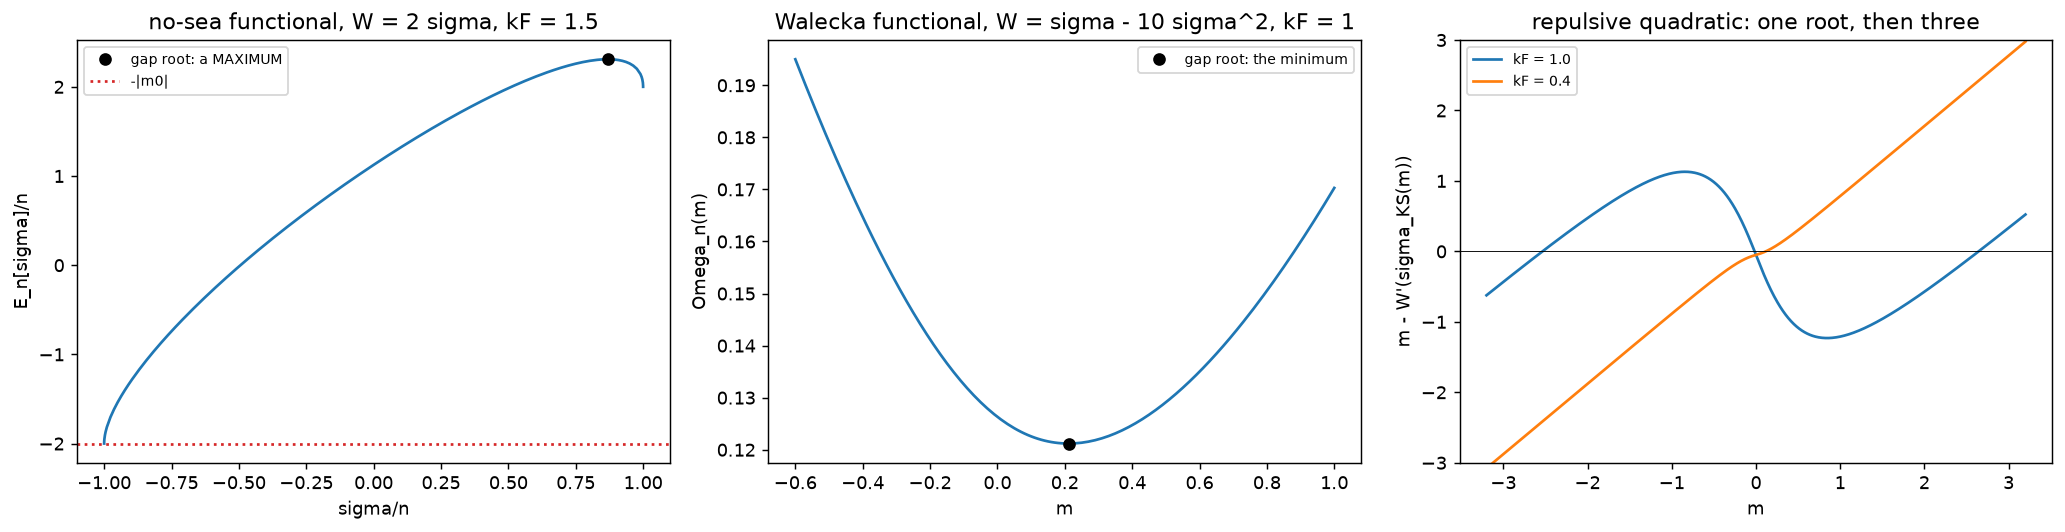
\includegraphics[width=\linewidth]{nb07_homogeneous.png}
  \caption{\texttt{nb07\_homogeneous.png}: the homogeneous Kohn--Sham ground state: the no-sea functional of
  $W=2\sigma$ ($k_F=1.5$, a maximum), the Walecka functional of $W=\sigma-10\sigma^2$ ($k_F=1$, the
  minimum), and the repulsive quadratic (one root, then three).}
  \label{fig:nb07homogeneous}
\end{figure}

\begin{figure}[htbp]
  \centering
  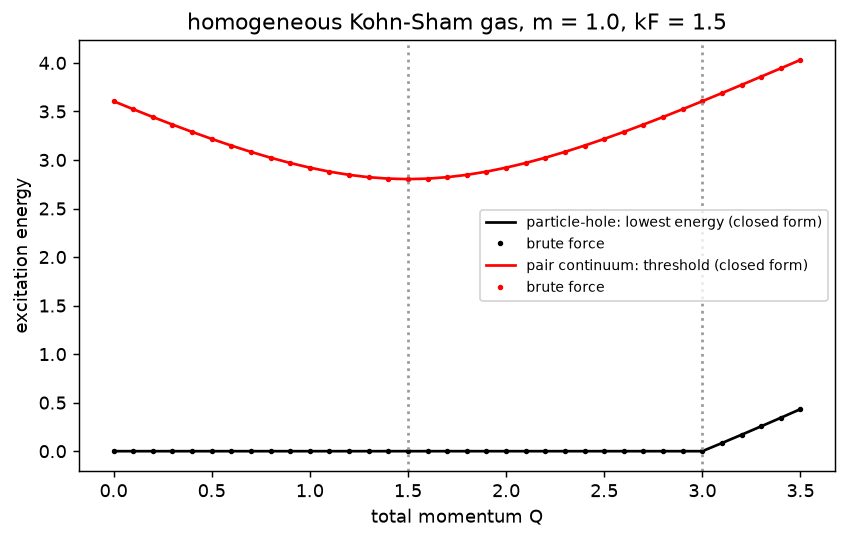
\includegraphics[width=0.6\linewidth]{nb07_excitations.png}
  \caption{\texttt{nb07\_excitations.png}: the particle--hole and pair excitation thresholds of the
  homogeneous gas ($m=1$, $k_F=1.5$) against the total momentum $Q$.}
  \label{fig:nb07excitations}
\end{figure}

\begin{figure}[htbp]
  \centering
  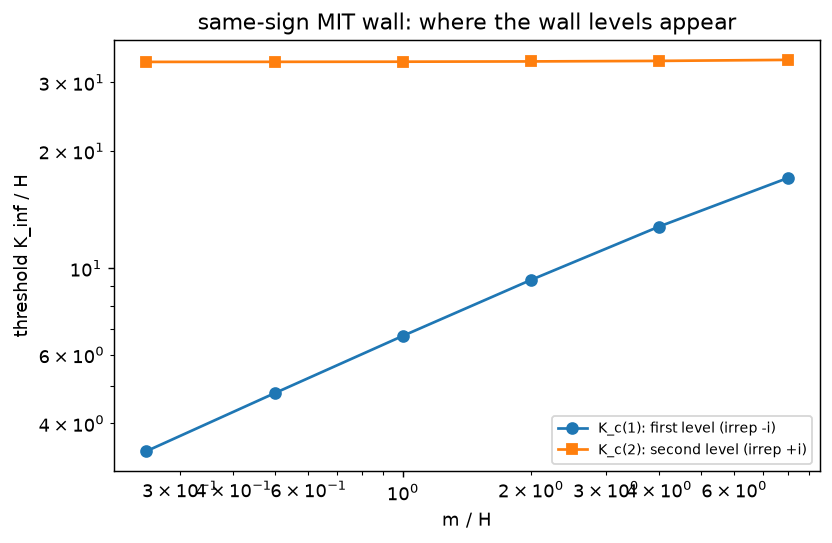
\includegraphics[width=0.6\linewidth]{nb07_thresholds.png}
  \caption{\texttt{nb07\_thresholds.png}: ``same-sign MIT wall: where the wall levels appear'': $K_c(1)$
  (irrep $-i$) and $K_c(2)$ (irrep $+i$) against $m/H$.}
  \label{fig:nb07thresholds}
\end{figure}

\begin{figure}[htbp]
  \centering
  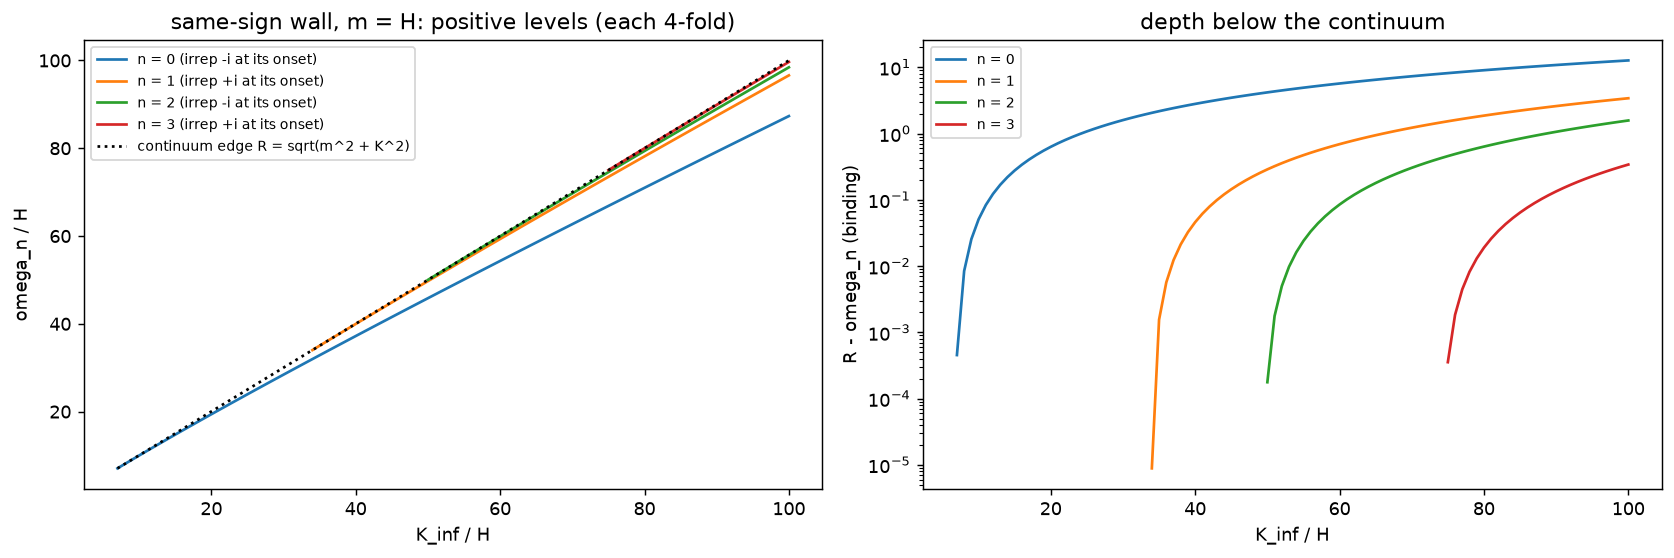
\includegraphics[width=0.95\linewidth]{nb07_dispersion.png}
  \caption{\texttt{nb07\_dispersion.png}: the positive levels $\omega_n(K)$ of the same-sign wall ($m=H$,
  each 4-fold) with the continuum edge $R=\sqrt{m^2+K^2}$, and their binding $R-\omega_n$.}
  \label{fig:nb07dispersion}
\end{figure}

\begin{figure}[htbp]
  \centering
  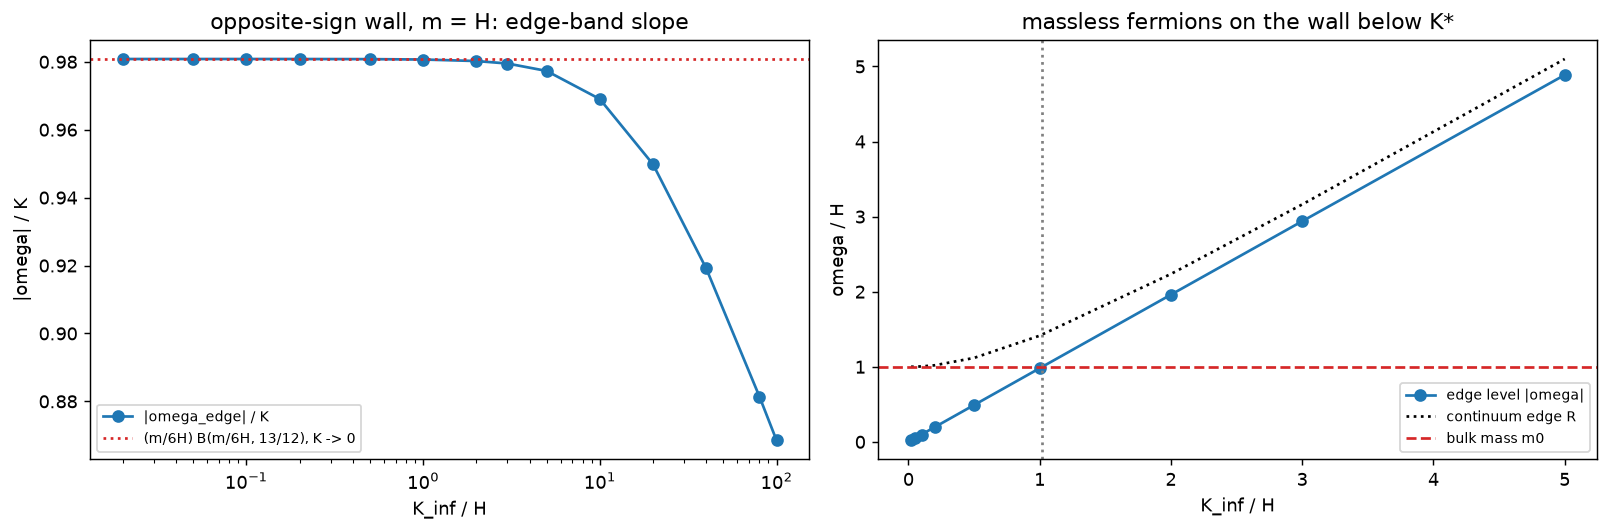
\includegraphics[width=0.95\linewidth]{nb07_edge_band.png}
  \caption{\texttt{nb07\_edge\_band.png}: the opposite-sign wall: $|\omega_{\mathrm{edge}}|/K$ against the
  closed-form slope $(m/6H)\,B(m/6H,13/12)$, and the edge level against the continuum edge and the bulk
  mass (``massless fermions on the wall below K*'').}
  \label{fig:nb07edge}
\end{figure}

\begin{figure}[htbp]
  \centering
  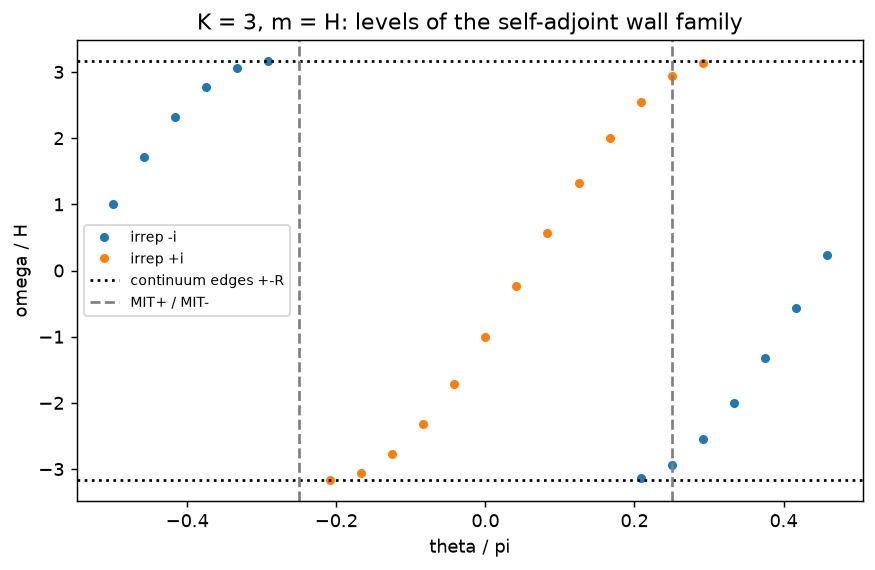
\includegraphics[width=0.6\linewidth]{nb07_theta.png}
  \caption{\texttt{nb07\_theta.png}: ``K = 3, m = H: levels of the self-adjoint wall family'' against
  $\theta/\pi$, both irreps, with the continuum edges and the MIT walls marked.}
  \label{fig:nb07theta}
\end{figure}

\begin{figure}[htbp]
  \centering
  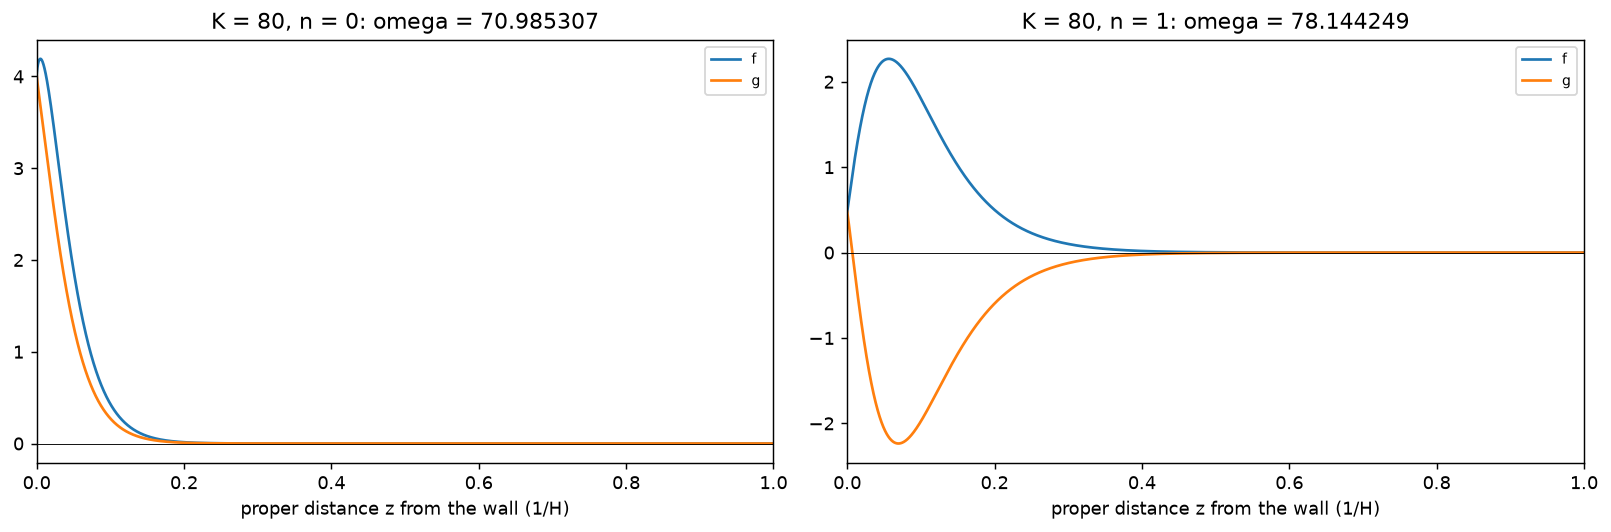
\includegraphics[width=0.95\linewidth]{nb07_wavefunctions.png}
  \caption{\texttt{nb07\_wavefunctions.png}: the orbitals $f(z)$, $g(z)$ of $n=0$ and $n=1$ at $K=80$
  against the proper distance from the wall.}
  \label{fig:nb07wavefunctions}
\end{figure}

\begin{figure}[htbp]
  \centering
  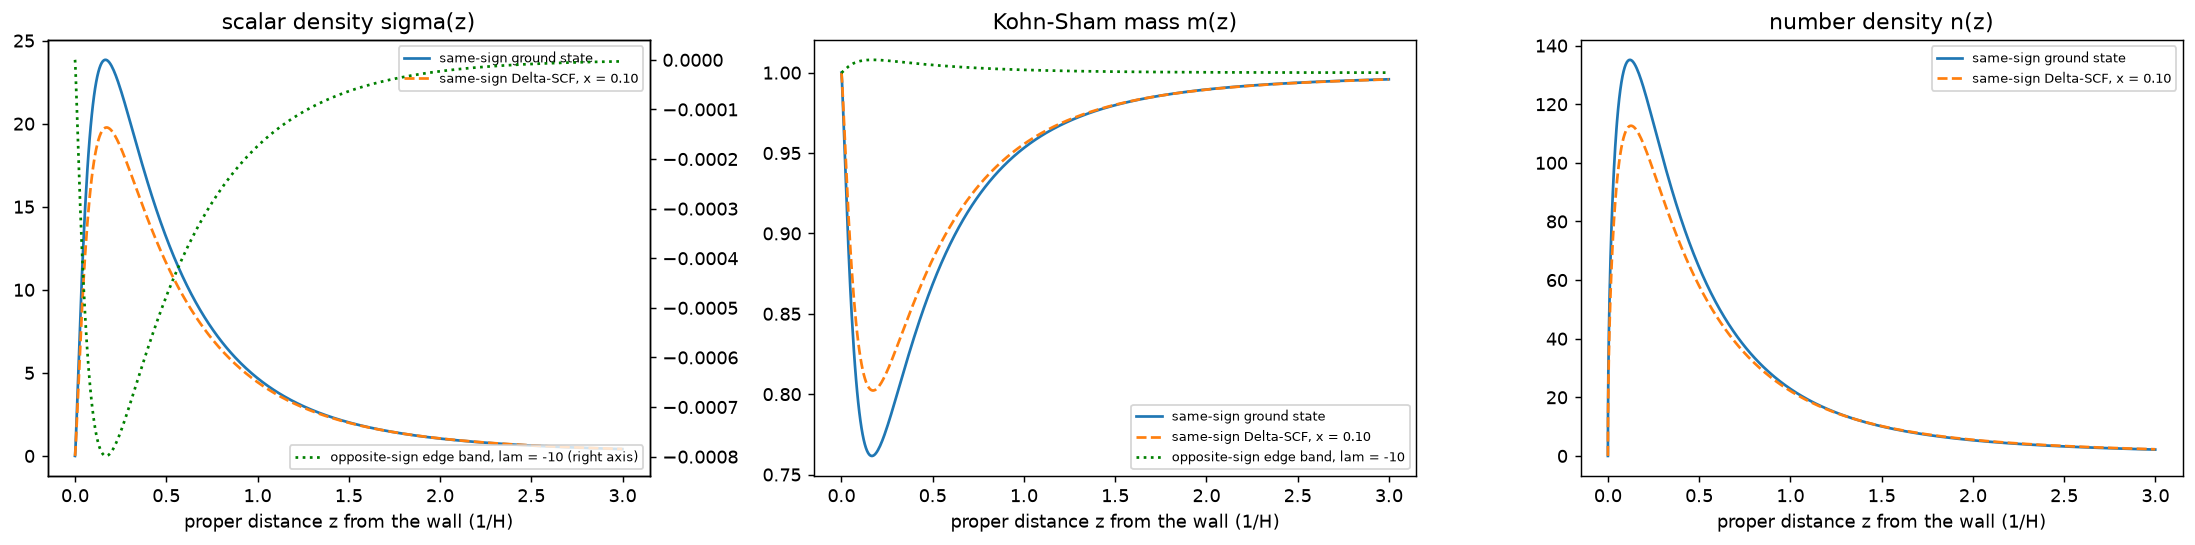
\includegraphics[width=\linewidth]{nb07_ks_profiles.png}
  \caption{\texttt{nb07\_ks\_profiles.png}: the Kohn--Sham profiles $\sigma(z)$, $m(z)$, $n(z)$ of the
  same-sign ground state, of the $\Delta$SCF state with $x=0.10$, and of the opposite-sign edge-band ground
  state ($\lambda=-10$).}
  \label{fig:nb07ksprofiles}
\end{figure}

\begin{figure}[htbp]
  \centering
  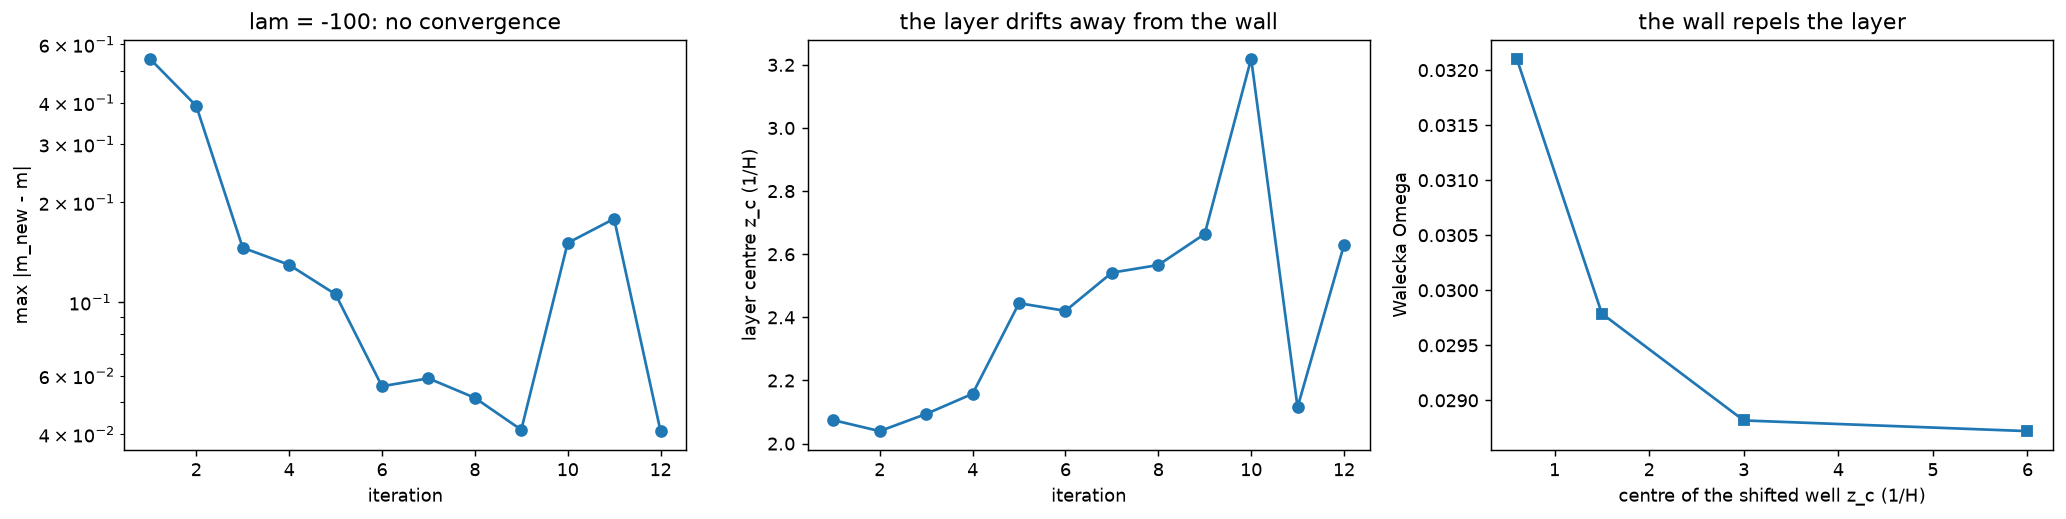
\includegraphics[width=\linewidth]{nb07_strong.png}
  \caption{\texttt{nb07\_strong.png}: strong attraction ($\lambda=-100$): the residual of the non-converging
  iteration, the layer centre drifting away from the wall, and the Walecka functional of the shifted well
  against its centre (``the wall repels the layer'').}
  \label{fig:nb07strong}
\end{figure}
\FloatBarrier

\begin{itemize}
  \item \textbf{Result files}: every table the notebook computes is also written as CSV under \cftt{results/} (\cftt{nb05\_*} 11 files, \cftt{nb06\_*} 37, \cftt{nb07\_*} 18), and \S{}6 of each notebook reads one back with plain Python and prints it (for example \cftt{nb06\_\allowbreak{}runs.\allowbreak{}csv:\allowbreak{} 29 rows,\allowbreak{} 34 columns} and a line per run with \cftt{a\_nr}, \cftt{Delta N\_\allowbreak{}eff(BBN)} and the CPL fit [nb06 \S{}6]).
  \item \textbf{The composed summary}: notebook 05 prints ten numbered statements, notebook 06 its answers to [1] and [2], notebook 07 nine numbered statements, each ending with a line that every statement is asserted (\cftt{every statement of this notebook is backed by the numbers above}, \cftt{every claim of the answers is asserted above}, \cftt{every statement of the summary is asserted in the cells above}). They are restated in sections~\ref{sec:4.5}--\ref{sec:4.8}.
\end{itemize}

\textbf{Troubleshooting} (what a failing notebook prints, and why): \cftt{The solver binary \dots{} does not exist} (the setup did not finish: run it again); an \cftt{AssertionError} naming \cftt{omega\_r0} in \S{}5 of 05 or 06 (the binary predates the \cftt{hbar} correction: rebuild it); \cftt{the Mathematica reference \dots{} is missing} in 06 (restore \cftt{reference/\allowbreak{}mathematica\_\allowbreak{}fable4d\_\allowbreak{}*.\allowbreak{}csv} with \cftt{git checkout}, or regenerate them, 6.3.7); notebook 07 stopping in its \S{}5.3 with \cftt{\dots{}fermion/\allowbreak{}waveguide\_\allowbreak{}T16.\allowbreak{}json is missing} (restore it with \cftt{git checkout -{}-{} fable-{}\allowbreak{}cosmology/\allowbreak{}fermion/\allowbreak{}waveguide\_\allowbreak{}T16.\allowbreak{}json}, or rewrite it, 6.6.1); \cftt{Kernel ...\allowbreak{} not found} or \cftt{No such kernel named python3} (run nbconvert from the \cftt{.venv}, which contains \cftt{ipykernel}); the Windows warnings \cftt{RuntimeWarning:\allowbreak{} Proactor event loop does not implement add\_\allowbreak{}reader \dots{}} and \cftt{[IPKernelApp] WARNING |\allowbreak{} Kernel is running over TCP without encryption} are warnings of the zmq and Jupyter libraries, not errors.

\needspace{6\baselineskip}
\subsection{Reproduce everything with one command}
\label{sec:6.8}

\begin{Verbatim}
bash "$(git rev-parse --show-toplevel)/fable-cosmology/run_all.sh"
\end{Verbatim}

\begin{Verbatim}
powershell -ExecutionPolicy Bypass -File fable-cosmology\run_all.ps1     # make Perl visible first (6.1)
\end{Verbatim}

\begin{itemize}
  \item \textbf{What it does} [file: \cftt{fable-{}\allowbreak{}cosmology/\allowbreak{}run\_\allowbreak{}all.\allowbreak{}sh}], after \cftt{setup.sh}, from any directory, under \cftt{set -{}euo pipefail} (it stops at the first failure): \cftt{==\allowbreak{} 1.\allowbreak{} solver tests} --- \cftt{cargo test -{}-{}release} in \cftt{rust/\allowbreak{}fable\_\allowbreak{}cosmo} (showing its last three lines) and in \cftt{rust/\allowbreak{}fable\_\allowbreak{}fermion} (showing its \cftt{running}, \cftt{test result}, \cftt{FAILED} and \cftt{panicked} lines); \cftt{==\allowbreak{} 2.\allowbreak{} notebooks} --- every \cftt{notebooks/\allowbreak{}0*.\allowbreak{}ipynb} in order, 01 to 07, executed in place with the \cftt{nbconvert} command of 6.7.2; \cftt{==\allowbreak{} 3.\allowbreak{} notebook requirements} --- \cftt{nbcheck.py}; \cftt{==\allowbreak{} 4.\allowbreak{} the paper} --- \cftt{latexmk -{}pdf -{}interaction=\allowbreak{}nonstopmode -{}halt-{}\allowbreak{}on-{}\allowbreak{}error fable\_\allowbreak{}cosmology.\allowbreak{}tex} in \cftt{fable-{}\allowbreak{}cosmology/\allowbreak{}latex/} (its output into \cftt{latex/\allowbreak{}latexmk.\allowbreak{}log}), then the PDF's \cftt{ls -{}la} line; and \cftt{==\allowbreak{} all done}. \cftt{run\_\allowbreak{}all.\allowbreak{}ps1} does the same, shows all of \cftt{cargo test}'s output, and throws on a failing \cftt{cargo test} of either solver (it checks \cftt{\$LASTEXITCODE}), a failing notebook, the checker or the paper build.
  \item \textbf{How long.} 12 min 18 s on 2026-09-25 with the seven notebooks (of which notebook 07 about 9 min and the \cftt{fable\_\allowbreak{}fermion} tests about 45 s; the committed execution of notebook 06 took 92.8 s); 3 min 35 s on 2026-09-24 before notebook 07 existed; 51 s (61 s in a fresh clone) before the fermion-fable work.
  \item \textbf{What it printed} on 2026-09-25 (Windows 11, Git Bash, the seven notebooks, 12 min 18 s), verbatim:
\end{itemize}

\begin{Verbatim}
== 1. solver tests
   rust/fable_cosmo

test result: ok. 7 passed; 0 failed; 0 ignored; 0 measured; 0 filtered out; finished in 0.00s

   rust/fable_fermion
running 23 tests
test result: ok. 23 passed; 0 failed; 0 ignored; 0 measured; 0 filtered out; finished in 38.31s
running 0 tests
test result: ok. 0 passed; 0 failed; 0 ignored; 0 measured; 0 filtered out; finished in 0.00s
running 11 tests
test result: ok. 11 passed; 0 failed; 0 ignored; 0 measured; 0 filtered out; finished in 0.93s
running 0 tests
test result: ok. 0 passed; 0 failed; 0 ignored; 0 measured; 0 filtered out; finished in 0.00s
== 2. notebooks
   executing notebooks/01_fableScalar_quintessence.ipynb
[NbConvertApp] Converting notebook notebooks/01_fableScalar_quintessence.ipynb to notebook
C:\Users\nsh\Documents\8-dim\Pre-Universe_14SEP26-77\fable-cosmology\.venv\Lib\site-packages\zmq\_future.py:718: RuntimeWarning: Proactor event loop does not implement add_reader family of methods required for zmq. Registering an additional selector thread for add_reader support via tornado. Use `asyncio.set_event_loop_policy(WindowsSelectorEventLoopPolicy())` to avoid this warning.
  self._get_loop()
[IPKernelApp] WARNING | Kernel is running over TCP without encryption. All communication (including code and outputs) is sent in plain text and is susceptible to eavesdropping. Use IPC transport or launch with kernel manager-provisioned CurveZMQ keys to enable transport encryption.
[NbConvertApp] Writing 475134 bytes to notebooks\01_fableScalar_quintessence.ipynb
   executing notebooks/02_fable_spinor.ipynb
[NbConvertApp] Converting notebook notebooks/02_fable_spinor.ipynb to notebook
   (the same two warning lines)
[NbConvertApp] Writing 532820 bytes to notebooks\02_fable_spinor.ipynb
   executing notebooks/03_pre-universe_dynamics.ipynb
[NbConvertApp] Converting notebook notebooks/03_pre-universe_dynamics.ipynb to notebook
   (the same two warning lines)
[NbConvertApp] Writing 1090050 bytes to notebooks\03_pre-universe_dynamics.ipynb
   executing notebooks/04_dark_matter_dark_energy.ipynb
[NbConvertApp] Converting notebook notebooks/04_dark_matter_dark_energy.ipynb to notebook
   (the same two warning lines)
[NbConvertApp] Writing 318320 bytes to notebooks\04_dark_matter_dark_energy.ipynb
   executing notebooks/05_fermion_fable_quantum_eos.ipynb
[NbConvertApp] Converting notebook notebooks/05_fermion_fable_quantum_eos.ipynb to notebook
   (the same two warning lines)
[NbConvertApp] Writing 734434 bytes to notebooks\05_fermion_fable_quantum_eos.ipynb
   executing notebooks/06_fable_primordial_gravity_8d.ipynb
[NbConvertApp] Converting notebook notebooks/06_fable_primordial_gravity_8d.ipynb to notebook
   (the same two warning lines)
[NbConvertApp] Writing 1412296 bytes to notebooks\06_fable_primordial_gravity_8d.ipynb
   executing notebooks/07_fable_dft_states.ipynb
[NbConvertApp] Converting notebook notebooks/07_fable_dft_states.ipynb to notebook
   (the same two warning lines)
[NbConvertApp] Writing 905839 bytes to notebooks\07_fable_dft_states.ipynb
== 3. notebook requirements

7/7 notebooks pass all eight requirements
== 4. the paper
-rw-r--r-- 1 nsh 197121 2835044 Sep 24 19:40 fable_cosmology.pdf
== all done
\end{Verbatim}

The only abbreviation is \cftt{(the same two warning lines)}, which stands for the zmq \cftt{RuntimeWarning} (two lines) and the \cftt{[IPKernelApp] WARNING}, repeated verbatim as after notebook 01; they are warnings of the zmq and Jupyter libraries on Windows, not of the notebooks, and they change no output. The empty line after \cftt{rust/\allowbreak{}fable\_\allowbreak{}cosmo} is the first of the three lines that \cftt{cargo test \dots{} |\allowbreak{} tail -{}n 3} keeps. The paper step lists the PDF; latexmk's own output is in \cftt{latex/\allowbreak{}latexmk.\allowbreak{}log}, which ends with \cftt{Latexmk:\allowbreak{} All targets (fable\_\allowbreak{}cosmology.\allowbreak{}pdf) are up-{}\allowbreak{}to-{}\allowbreak{}date} when nothing changed (after three pdflatex passes the first time). - \textbf{Success:} \cftt{==\allowbreak{} all done} with exit code 0, \cftt{7/\allowbreak{}7 notebooks pass all eight requirements}, and \cftt{git diff -{}-{}stat -{}-{} fable-{}\allowbreak{}cosmology/\allowbreak{}results} empty (6.5).

\needspace{6\baselineskip}
\subsection{The LaTeX build}
\label{sec:6.9}

\begin{Verbatim}
bash "$(git rev-parse --show-toplevel)/provenance-latex/build_all.sh"
\end{Verbatim}

\begin{Verbatim}
powershell -ExecutionPolicy Bypass -File provenance-latex\build_all.ps1
\end{Verbatim}

\begin{itemize}
  \item \textbf{What it does} [file: \cftt{provenance-{}\allowbreak{}latex/\allowbreak{}build\_\allowbreak{}all.\allowbreak{}sh}]. For each of the three LaTeX twins of the provenance pages of 2026-09-24 --- \cftt{PROVENANCE-{}14-{}FERMION-{}\allowbreak{}FABLE-{}\allowbreak{}CANONICAL-{}\allowbreak{}QUANTIZATION}, \cftt{PROVENANCE-{}15-{}FERMION-{}\allowbreak{}FABLE-{}\allowbreak{}AND-{}\allowbreak{}THE-{}\allowbreak{}PRIMORDIAL-{}\allowbreak{}GRAVITATIONAL-{}\allowbreak{}FIELD} and \cftt{PROVENANCE-{}16-{}THE-{}\allowbreak{}COMPLETE-{}\allowbreak{}SOLUTION-{}\allowbreak{}AND-{}\allowbreak{}ITS-{}\allowbreak{}COMMANDS} (the twin of this page) --- it runs \cftt{latexmk -{}pdf -{}interaction=\allowbreak{}nonstopmode -{}halt-{}\allowbreak{}on-{}\allowbreak{}error \textless{}doc\textgreater{}.\allowbreak{}tex} (as many pdflatex passes as the cross-references need), with the output in \cftt{provenance-{}\allowbreak{}latex/\allowbreak{}\textless{}doc\textgreater{}.\allowbreak{}latexmk.\allowbreak{}log}; it stops on the first failure, printing \cftt{FAILED;\allowbreak{} see provenance-{}\allowbreak{}latex/\allowbreak{}\textless{}doc\textgreater{}.\allowbreak{}latexmk.\allowbreak{}log and \textless{}doc\textgreater{}.\allowbreak{}log}; it warns (\cftt{WARNING:\allowbreak{} undefined references in \textless{}doc\textgreater{}.\allowbreak{}log}) if the \cftt{.log} contains ``undefined'' or ``Rerun to get''; and it lists each PDF. Every document begins with \cftt{\textbackslash{}input\{preamble\}} (\cftt{provenance-{}\allowbreak{}latex/\allowbreak{}preamble.\allowbreak{}tex}: pdfLaTeX, Latin Modern, A4, 2.5 cm margins, and macros for the notebook's objects, with separate symbols for the classical conjugation \cftt{\textbackslash{}cconj} and the Hilbert adjoint \cftt{\textbackslash{}hadj}); the generated fragments of \cftt{provenance-{}\allowbreak{}latex/\allowbreak{}generated/} are \cftt{\textbackslash{}input} where the equations are quoted. \cftt{build\_\allowbreak{}all.\allowbreak{}ps1} does the same in PowerShell and throws on a failing \cftt{latexmk}. MiKTeX's \cftt{latexmk} needs Perl on the \cftt{PATH}; Git for Windows ships one (\cftt{\$env:\allowbreak{}PATH +=\allowbreak{} \textquotedbl{};\allowbreak{}C:\allowbreak{}\textbackslash{}Program Files\textbackslash{}Git\textbackslash{}usr\textbackslash{}bin\textquotedbl{}} in PowerShell).
  \item \textbf{What it prints:} \cftt{== \textless{}doc\textgreater{}} and an \cftt{ls -{}la} line per document, and finally \cftt{==\allowbreak{} all three PDFs built}.
  \item \textbf{Success:} exit code 0 and that last line; the \cftt{.log} of each document free of errors and undefined references, and no overfull box worse than 10pt (\cftt{grep -{}n -{}E \textquotedbl{}\textasciicircum{}!|\allowbreak{}undefined|\allowbreak{}Overfull\textquotedbl{} \textless{}doc\textgreater{}.\allowbreak{}log}). The twin of the page of Effort A was built this way when it was committed: 110 pages, no errors, no undefined references, no overfull box above 5.5pt [commit fee5603]. The output of the build of all three twins on the final pushed state is recorded with the fresh-clone verification (section~\ref{sec:7}).
\end{itemize}

The paper of Effort 0 is built the same way from \cftt{fable-{}\allowbreak{}cosmology/\allowbreak{}latex}:

\begin{Verbatim}
cd "$(git rev-parse --show-toplevel)/fable-cosmology/latex"
latexmk -pdf -interaction=nonstopmode -halt-on-error fable_cosmology.tex
\end{Verbatim}

A clean build ends with \cftt{Output written on fable\_\allowbreak{}cosmology.\allowbreak{}pdf (24 pages,\allowbreak{} \dots{})} in \cftt{fable\_\allowbreak{}cosmology.\allowbreak{}log}, with no errors, no undefined references and no overfull boxes; \cftt{latexmk -{}c} removes the by-products (which git ignores). Its 16 figures are byte-identical copies of the notebooks' PNGs in \cftt{latex/\allowbreak{}figures/}.

\needspace{6\baselineskip}
\subsection{Git: commit, push, check the remote, clone afresh}
\label{sec:6.10}

\textbf{Commit and push} (every commit of the work was made this way; the notebook's two \cftt{.mx} files are restored first, 6.3.4):

\begin{Verbatim}
cd "$(git rev-parse --show-toplevel)"
git status --short                                   # what changed
git add <the files of the step>                      # named files, never a blanket add
git commit -m "<what the step adds or fixes>" -m "<details>" -m "Co-Authored-By: Claude Opus 5.5 <noreply@anthropic.com>"
git push origin main
\end{Verbatim}

\cftt{origin} is \cftt{https:\allowbreak{}//\allowbreak{}github.\allowbreak{}com/\allowbreak{}once-{}\allowbreak{}ere/\allowbreak{}Pre-{}\allowbreak{}Universe\_\allowbreak{}with\_\allowbreak{}Claude.\allowbreak{}git}; the remote named \cftt{upstream} (the author's other repository) is never pushed to. Since pull request \#1 (section~\ref{sec:2.2}) every commit went directly to \cftt{main}.

\textbf{Check that the remote has what was pushed:}

\begin{Verbatim}
cd "$(git rev-parse --show-toplevel)"
git fetch origin
git rev-parse HEAD origin/main              # both must print the same hash
git ls-remote origin refs/heads/main        # the hash GitHub serves for main
git status --short                          # what is not yet committed
\end{Verbatim}

When this page was written (2026-09-25), \cftt{git ls-{}\allowbreak{}remote origin refs/\allowbreak{}heads/\allowbreak{}main} printed

\begin{Verbatim}
16711556effcf920b28a606f4c365149f126dd4e	refs/heads/main
\end{Verbatim}

which is the local \cftt{main} (\cftt{git rev-{}\allowbreak{}parse HEAD} printed the same hash): \cftt{1671155}, ``Record the final notebook run: 217 Input cells, 644/644 assertions, 0 messages''. Earlier checks printed \cftt{bc04ed16096e134857111ae16df5220d4ff18435} (about 21:28 PDT on 2026-09-24) and \cftt{2bc936d0dfd6f6c1243214fc6b1b9947f5bded6e} (23:26 PDT). The final commits and the \cftt{ls-{}remote} line of the final push are recorded in section~\ref{sec:7.4}.

\textbf{Clone afresh and verify} (\cftt{\textless{}scratch\textgreater{}} is any empty directory outside the repository; section~\ref{sec:7} records the results):

\begin{Verbatim}
cd <scratch>
git clone https://github.com/once-ere/Pre-Universe_with_Claude.git fresh
cd fresh
git log --oneline -1                                   # the hash of the pushed main
cd claude-fable
cp claude-fable_Einstein-Rosen-2-Planes.nb committed.nb
python build_tools.py                                  # the four lines of 6.3.1
cmp claude-fable_Einstein-Rosen-2-Planes.nb committed.nb && echo "notebook rebuilds byte for byte"
wolframscript -file verify_nb.wls                      # 6.3.2
cd ../fable-cosmology
bash setup.sh                                          # 6.1
bash run_all.sh                                        # 6.8: both crates' tests, notebooks 01-07, nbcheck, the paper
git diff --stat -- results                             # empty: every result file reproduced byte for byte
.venv/Scripts/python.exe fermion/crosscheck.py --jobs 6
(cd fermion && ../.venv/Scripts/python.exe waveguide.py validate)
cd ../claude-fable
wolframscript -file run_from_nb.wls > fresh_run.log 2>&1      # after run_all.sh, so the Rust CSVs exist
sed -n '/RUN SUMMARY/,$p' fresh_run.log                # 217 cells, 644/644, cells w/ msgs 0
diff <(grep '^  PASS' fresh_run.log) <(grep '^  PASS' run_fermion_fable_final.log) && echo "every label identical"
git checkout -- claude-fable_Einstein-Rosen-2-Planes-eLa.mx claude-fable_Einstein-Rosen-2-Planes-eLazt.mx
cd .. && bash provenance-latex/build_all.sh            # 6.9
\end{Verbatim}

\textbf{The delivered copy of the notebook} outside the repository, \cftt{C:\allowbreak{}/\allowbreak{}Users/\allowbreak{}nsh/\allowbreak{}Documents/\allowbreak{}8-{}dim/\allowbreak{}claude-{}\allowbreak{}fable\_\allowbreak{}Einstein-{}\allowbreak{}Rosen-{}2-{}Planes.\allowbreak{}nb}, is refreshed from \cftt{claude-{}\allowbreak{}fable/} whenever the notebook changes, next to the author's two helper packages. When this page was written it was 545408 bytes and byte-identical to the repository's notebook (\cftt{cmp} reported no difference); when the page of Effort A was written it was still the 2026-09-16 version (273270 bytes).

% ===============================================================================================
\needspace{6\baselineskip}
\section{Verification of the repository: the push, and a fresh clone of it}
\label{sec:7}

\needspace{6\baselineskip}
\subsection{What was pushed, and what was not yet, when this page was written}
\label{sec:7.1}

\needspace{8\baselineskip}
\textbf{The commits of the work} (\cftt{git log -{}-{}date=\allowbreak{}iso}, PDT; every one pushed to \cftt{origin/\allowbreak{}main} of \cftt{https:\allowbreak{}//\allowbreak{}github.\allowbreak{}com/\allowbreak{}once-{}\allowbreak{}ere/\allowbreak{}Pre-{}\allowbreak{}Universe\_\allowbreak{}with\_\allowbreak{}Claude.\allowbreak{}git}):

{\footnotesize
\setlength{\tabcolsep}{3pt}
\begin{longtable}{@{}p{0.090\linewidth}p{0.130\linewidth}p{0.060\linewidth}p{0.640\linewidth}@{}}
\toprule
\raggedright commit & \raggedright time & \raggedright effort & \raggedright what it contains \tabularnewline
\midrule
\endhead
\raggedright \cftt{e34d454} & \raggedright 2026-09-24 18:52:36 & \raggedright 0 & \raggedright the 2026-09-16 work as it stood: Part VI (172 Input cells, 358/358), \cftt{fable\_\allowbreak{}cosmo}, notebooks 01--04, results, references, setup and run scripts (section~\ref{sec:2.1}) \tabularnewline
\raggedright \cftt{028b379} & \raggedright 19:24:32 & \raggedright 0 & \raggedright the reference generator runs without underflow messages; pull request \#1, merged 19:32:10 (section~\ref{sec:2.2}) \tabularnewline
\raggedright \cftt{2f6d322} & \raggedright 19:57:29 & \raggedright 0 & \raggedright the gaps of 2026-09-16 closed: student instructions, the paper, the provenance page of that work, seven design corrections, \cftt{setup.sh}, \cftt{run\_\allowbreak{}all.\allowbreak{}ps1}; a fresh local clone ran \cftt{setup.sh} and \cftt{run\_all.sh} end to end (section~\ref{sec:2.3}) \tabularnewline
\raggedright \cftt{8459c57} & \raggedright 20:02:04 & \raggedright B & \raggedright a work-in-progress snapshot of the solver crate \cftt{fable\_\allowbreak{}fermion} \tabularnewline
\raggedright \cftt{e130337} & \raggedright 20:14:25 & \raggedright B & \raggedright a second work-in-progress snapshot of that crate \tabularnewline
\raggedright \cftt{0a789e2} & \raggedright 20:17:18 & \raggedright C & \raggedright the LaTeX build tree of the three provenance pages: \cftt{provenance-{}\allowbreak{}latex/\allowbreak{}preamble.\allowbreak{}tex}, \cftt{build\_\allowbreak{}all.\allowbreak{}sh}, \cftt{build\_\allowbreak{}all.\allowbreak{}ps1}; \cftt{.gitignore} names each document's \cftt{.log} and \cftt{.\allowbreak{}latexmk.\allowbreak{}log}; a minimal test document compiled with no warnings \tabularnewline
\raggedright \cftt{d0f2a99} & \raggedright 20:18:53 & \raggedright C & \raggedright \cftt{build\_\allowbreak{}all.\allowbreak{}sh} tracked without the executable bit (mode 100644), like the repository's other scripts \tabularnewline
\raggedright \cftt{c5892bd} & \raggedright 20:38:49 & \raggedright B & \raggedright the finished solver \cftt{fable\_\allowbreak{}fermion} (21 + 8 tests), the independent \cftt{crosscheck.\allowbreak{}py} (every run below $10^{-8}$), \cftt{report.py} \tabularnewline
\raggedright \cftt{4fdfc40} & \raggedright 20:47:28 & \raggedright A & \raggedright Part VII of the notebook (198 Input cells, 528/528, 0 cells with messages), its log, the checker's log, the TeX export and its fourteen generated files \tabularnewline
\raggedright \cftt{b7ea18d} & \raggedright 20:48:42 & \raggedright A & \raggedright the wording correction of an earlier provenance page (section~\ref{sec:5.8}, item 6) \tabularnewline
\raggedright \cftt{bc04ed1} & \raggedright 21:24:04 & \raggedright B & \raggedright Part VIII of the notebook (217 Input cells, 642/642), its log, and the Mathematica reference runs of the coupled system \tabularnewline
\raggedright \cftt{18a2501} & \raggedright 22:13:42 & \raggedright B & \raggedright the wall-state solver, its derivation (94/94), its Mathematica check (11/11), its report \tabularnewline
\raggedright \cftt{fee5603} & \raggedright 22:31:20 & \raggedright A, C & \raggedright the page of Effort A (draft) and its LaTeX twin and PDF (110 pages) \tabularnewline
\raggedright \cftt{2bc936d} & \raggedright 23:12:51 & \raggedright B & \raggedright six solver defects fixed, 34/34 tests (section~\ref{sec:5.8}, item 4) \tabularnewline
\raggedright \cftt{aca5102} & \raggedright 2026-09-25 00:23:46 & \raggedright B, 0 & \raggedright notebooks 05--07 executed, their 90 result files, the integration (nbcheck 7/7, \cftt{run\_all.sh} passing), the fermion sections of the student instructions, \cftt{waveguide\_\allowbreak{}T16.\allowbreak{}json} committed, the \cftt{nbgen.py} corrections of notebooks 01--04 \tabularnewline
\raggedright \cftt{1671155} & \raggedright 00:28:54 & \raggedright B & \raggedright the final full run of the notebook, \cftt{claude-{}\allowbreak{}fable/\allowbreak{}run\_\allowbreak{}fermion\_\allowbreak{}fable\_\allowbreak{}final.\allowbreak{}log} (217 Input cells, 644/644, 0 messages, 208.715 s, 46 witnesses) \tabularnewline
\bottomrule
\end{longtable}
}

When this page was written, \cftt{git ls-{}\allowbreak{}remote origin refs/\allowbreak{}heads/\allowbreak{}main} printed \cftt{16711556effcf920b28a606f4c365149f126dd4e	refs/\allowbreak{}heads/\allowbreak{}main}, the local \cftt{main}. Everything that exists as code, notebook, log, result file or generated file is in that pushed history. \textbf{Not yet committed} at that moment: this page, the page of Effort B and the LaTeX twins and PDFs of the pages of Efforts B and C, and an update of the repository's front page (its table of the notebook's Parts, the final counts, the table of provenance pages). None of the numbers on this page is taken from an uncommitted file: every one comes from the committed notebooks, result files, logs, reports and commit messages named next to it. They are committed together at the end of the work, and that final state is what the fresh clone verifies.

\needspace{6\baselineskip}
\subsection{What the fresh-clone verification consists of}
\label{sec:7.2}

The final pushed \cftt{main} is cloned into an empty directory outside the repository, and everything is rebuilt and re-run there from nothing --- a new virtual environment, a new engine clone from GitHub, new builds --- with the commands of section~\ref{sec:6.10}, in this order, each result compared with the committed record:

{\small
\begin{longtable}{@{}p{0.050\linewidth}p{0.380\linewidth}p{0.480\linewidth}@{}}
\toprule
\raggedright step & \raggedright command & \raggedright compared with \tabularnewline
\midrule
\endhead
\raggedright 1 & \raggedright \cftt{git clone https:\allowbreak{}//\allowbreak{}github.\allowbreak{}com/\allowbreak{}once-{}\allowbreak{}ere/\allowbreak{}Pre-{}\allowbreak{}Universe\_\allowbreak{}with\_\allowbreak{}Claude.\allowbreak{}git fresh}; \cftt{git log -{}-{}oneline -{}1} & \raggedright the hash \cftt{git ls-{}\allowbreak{}remote} reports for \cftt{main} \tabularnewline
\raggedright 2 & \raggedright \cftt{python build\_\allowbreak{}tools.\allowbreak{}py} in \cftt{claude-{}\allowbreak{}fable/}; \cftt{cmp} against the committed notebook & \raggedright byte-identical \cftt{.nb} and \cftt{run\_\allowbreak{}all.\allowbreak{}wls} (6.3.1) \tabularnewline
\raggedright 3 & \raggedright \cftt{wolframscript -{}file verify\_\allowbreak{}nb.\allowbreak{}wls} & \raggedright the output of 6.3.2 (\cftt{input cells that FAIL to parse:\allowbreak{} \{\}}) \tabularnewline
\raggedright 4 & \raggedright \cftt{bash fable-{}\allowbreak{}cosmology/\allowbreak{}setup.\allowbreak{}sh} & \raggedright \cftt{==\allowbreak{} setup complete}, both \cftt{-{}-{}version} lines (6.1) \tabularnewline
\raggedright 5 & \raggedright \cftt{bash fable-{}\allowbreak{}cosmology/\allowbreak{}run\_\allowbreak{}all.\allowbreak{}sh} & \raggedright \cftt{test result:\allowbreak{} ok.\allowbreak{} 7 passed}; \cftt{23 passed}, \cftt{11 passed}; the seven notebooks executed; \cftt{7/\allowbreak{}7 notebooks pass all eight requirements}; the paper built; \cftt{==\allowbreak{} all done} (6.8) \tabularnewline
\raggedright 6 & \raggedright \cftt{git diff -{}-{}stat -{}-{} fable-{}\allowbreak{}cosmology/\allowbreak{}results} & \raggedright empty: all 149 result files (59 of notebooks 01--04, 63 of 05 and 06, 27 of 07) reproduced byte for byte; any CSV that differs compared column by column (6.5) \tabularnewline
\raggedright 7 & \raggedright \cftt{python fermion/\allowbreak{}crosscheck.\allowbreak{}py -{}-{}jobs 6}; \cftt{python fermion/\allowbreak{}waveguide.\allowbreak{}py validate} & \raggedright \cftt{CROSSCHECK PASSED:\allowbreak{} every difference \textless{} 1e-{}06}; \cftt{VALIDATION:\allowbreak{} 64 of 64 PASS} \tabularnewline
\raggedright 8 & \raggedright \cftt{wolframscript -{}file run\_\allowbreak{}from\_\allowbreak{}nb.\allowbreak{}wls} (after step 5, so the Rust CSVs exist) & \raggedright \cftt{cells evaluated :\allowbreak{} 217}, \cftt{assertions run \ :\allowbreak{} 644}, \cftt{passed \ \ \ \ \ \ \ \ \ :\allowbreak{} 644}, \cftt{FAILED \ \ \ \ \ \ \ \ \ :\allowbreak{} 0}, \cftt{cells w/\allowbreak{} msgs \ \ :\allowbreak{} 0}; every \cftt{PASS} label identical to \cftt{claude-{}\allowbreak{}fable/\allowbreak{}run\_\allowbreak{}fermion\_\allowbreak{}fable\_\allowbreak{}final.\allowbreak{}log} (6.3.5) \tabularnewline
\raggedright 9 & \raggedright \cftt{bash provenance-{}\allowbreak{}latex/\allowbreak{}build\_\allowbreak{}all.\allowbreak{}sh} & \raggedright \cftt{==\allowbreak{} all three PDFs built}, no errors, no undefined references, no overfull box worse than 10pt (6.9) \tabularnewline
\raggedright 10 & \raggedright \cftt{git status -{}-{}short} after restoring the two \cftt{.mx} files & \raggedright only the re-executed notebooks (timestamps) and nothing else \tabularnewline
\bottomrule
\end{longtable}
}

\needspace{6\baselineskip}
\subsection{The results of the fresh-clone verification}
\label{sec:7.3}

\texttt{\{\{FRESH-CLONE\}\}}

\needspace{6\baselineskip}
\subsection{The final push}
\label{sec:7.4}

\texttt{\{\{FINAL-PUSH\}\}}

% ===============================================================================================
\needspace{6\baselineskip}
\section{What remains open}
\label{sec:8}

This is the honest list: what the work did not do, what it assumed without deriving, and where its answers stop. Each item names the section where it is discussed.

\needspace{6\baselineskip}
\subsection{Physics that was not done}
\label{sec:8.1}

\begin{enumerate}
  \item \textbf{The Maxwell construction.} For the repulsive quadratic potential ($g_q > 0$) the Kohn--Sham ground state jumps between gap branches at $a = 0.9962806544$ --- a first-order transition. Energy conservation across it needs the Maxwell (coexistence) construction, which the solver does not implement; it \textbf{refuses} the run instead (sections~\ref{sec:4.7.11}, \ref{sec:6.4.8}). The physics of that transition --- coexisting phases, latent heat, bubbles --- is not examined.
  \item \textbf{Exchange and correlation.} $E_{\mathrm{xc}}$ is neglected everywhere (the Hartree mean field). That is exact for the author's mass term, which is free, but for a nonlinear $W$ the Fock exchange of the contact interaction is $1/g$ of the Hartree term only for $k_F \ll m$, and of order one or larger for $k_F \gtrsim m$, the early-universe regime. The ratio of the interaction energy to $3 P_{\mathrm{KS}}$, which alone controls the neglect there, was \textbf{not computed} in the runs (section~\ref{sec:4.5.12}).
  \item \textbf{The vacuum energy is fine-tuned, not solved.} For a constant mass the Dirac-sea energy is a constant, absorbed into $V_0$ as a bare cosmological constant: the cosmological-constant problem is not addressed. For a mass-varying potential the runs read $W$ as the fully renormalized effective potential, which absorbs the sea energy only by fine-tuning: its variation along the runs is $1.31\times10^{13}$ to $2.87\times10^{16}$ times the total density at $a \geq 0.3$ (at least $3.79\times10^{9}$ over the scans). The other option --- including $\Delta E_{\mathrm{vac}}(m)$ in $\rho$ and in the gap equation --- was not run (sections~\ref{sec:3.7.3}, \ref{sec:4.5.11}, \ref{sec:4.8.1}).
  \item \textbf{The origin of the stabilizer is unknown.} Every result of Effort B rests on the stabilized model \cftt{fable4d}, whose hidden sheet is held by $P_{\mathrm{stab}} = -F/2$: a Lagrange multiplier with zero energy density, not a stress derived from any field, which \textbf{violates the null energy condition along $x_{0}$} wherever dust is present ($\rho + P_C = -\rho_{\mathrm{dust}}/2$; negative on every output row of every stabilized run). Without it (\cftt{fable8d}) the Newton constant varies by $6.5\times10^{8}$ to $1.9\times10^{17}$ and the model is excluded. What physical mechanism could stabilize the hidden sheet is not known (sections~\ref{sec:4.7.1}, \ref{sec:4.7.10}).
  \item \textbf{The strong-coupling wall state.} At $\lambda = -100$ homogeneous matter is self-bound, but the Kohn--Sham iteration at the same-sign wall does \textbf{not converge} (residual $4.1\times10^{-2}$ after 12 iterations; the layer drifts from $z_c = 2.07$ to $2.63$), and the wall repels the layer. A position-constrained iteration, to map $E(z_c)$ self-consistently, was not done; only a rigid-shift upper bound was computed (section~\ref{sec:4.6.6}).
  \item \textbf{The same-sign wall's self-consistent state is not a ground state.} At $\lambda = -0.01$, $N_s = 100$ the iteration converges, but $\mu - m_0 = 10.696 > 0$ (bulk states lie below the Fermi level) and the Walecka functional is not stationary ($d\Omega/ds=-48.3$). A grand-canonical treatment with a bulk fable density was not done (section~\ref{sec:4.6.6}).
  \item \textbf{Perturbations were not examined.} Everything is homogeneous background cosmology. Every massive mass-varying case has a negative adiabatic sound speed ($c_s^{2}$ down to $-0.611$ for \cftt{power nu =\allowbreak{} 0.236}, $-27$ for $\nu = 0.5$, $-21.8$ for \cftt{expdamp}, $-47.1$ for \cftt{quadratic}, $-0.364$ in Part VIII's case), which signals an instability of perturbations that is stated but not followed; the free-streaming bound ($m\approx1.1\text{--}1.8\,\mathrm{keV}$) is a velocity-matching estimate, not a transfer-function computation; structure formation, the CMB and lensing are not computed (sections~\ref{sec:4.7.6}, \ref{sec:4.7.9}).
  \item \textbf{Renormalized $\langle T\rangle$ on a time-dependent background.} $\langle0|{:}T{:}|0\rangle=0$ holds only for a static background or adiabatically; a conserved renormalized expectation on an $x_{4}$-dependent background needs adiabatic subtraction or point-splitting, which was not carried out (section~\ref{sec:3.7.3}).
  \item \textbf{Reflection positivity} of the $J$-quantization was claimed in the design, not verified, and dropped (section~\ref{sec:5.2}, QK-5).
  \item \textbf{Other wall conditions.} Only the flavour-symmetric, charge-conjugation-invariant MIT walls $Q = \pm 1$ were solved; the mixed walls $P = T_{16}[0] Q$ and the non-$J$-preserving covariant walls were described, not solved (section~\ref{sec:4.6.3}).
\end{enumerate}

\needspace{6\baselineskip}
\subsection{Assumptions made, not derived}
\label{sec:8.2}

\begin{enumerate}
  \item \textbf{$a_{4}$ is free.} It is never given a value; nothing in the work determines it. The wall states are computed at a frozen $a_{4}$ (the adiabatic approximation, with $K_\infty=k\,e^{a_4}$), and the cosmology uses the asymptotic region of the generalized frame, not $a_{4}$ (sections~\ref{sec:3.1.11}, \ref{sec:4.3.3}, \ref{sec:4.6.3}).
  \item \textbf{The present universe is the asymptotic Bianchi-I region} of the generalized warped frame, valid when $24 (H/H_A)^{2} \cot^{2}/C^{2} \ll 1$; the frozen and dust-driven solutions solve the warped equations only up to $O(e^{-12Hz})$ terms, including an $x_{0}$-momentum flux (sections~\ref{sec:4.3.3}, \ref{sec:4.3.4}).
  \item \textbf{The (0,4) equation singles out, but does not derive, the author's volume-preserving structure} (with $C = 1$ and $T^4{}_0=0$; with $C$ dynamical, positive-energy expansion is allowed) (section~\ref{sec:4.3.2}).
  \item \textbf{The admissible theory is a truncation} to fields independent of $x_5..x_7$ with a finite hidden coordinate volume $V_{\mathrm{hid}}$; compactifying the timelike $x_5..x_7$ produces closed timelike curves; $x_{0}$ is taken as compactified at large $z$ with a Kaluza--Klein gap $1/L_0 \gg T_{\max}$, so that all matter is in zero modes (sections~\ref{sec:3.5.4}, \ref{sec:4.7.1}).
  \item \textbf{The beginning of the present universe} is not fixed by the pre-universe: $a_i \leq \min(10^{-10}, 0.01 a_{\mathrm{nr}}(m))$ is chosen on physical grounds (before nucleosynthesis, fable ultra-relativistic) and shown not to matter; $g_*(T)$ is not followed (a factor $0.46\text{--}0.83$ on $\rho_r a^{4}$ at $a \approx 10^{-12}$) (section~\ref{sec:4.7.2}).
  \item \textbf{Semiclassical gravity} with the Kohn--Sham expectation value as the source; the split of the fable into dark matter and dark energy is a \textbf{convention} (the condensate $\rho_U$ is an 8-dimensional vacuum energy) (sections~\ref{sec:4.2.1}, \ref{sec:4.5.10}).
\end{enumerate}

\needspace{6\baselineskip}
\subsection{Where the answers stop}
\label{sec:8.3}

\begin{itemize}
  \item \textbf{[1]} A time-varying dark-energy equation of state exists formally in the stabilized model with a mass-varying potential, but in no run is it viable: with a bare $\Lambda$ the inferred dark energy is a cosmological constant; with a mass-varying potential the fable's own $w_f$ never goes below \ensuremath{-}1, while the observer-inferred dark energy has a pole and is phantom or crosses \ensuremath{-}1 (apparent, from the dark-sector energy exchange); the fable is massless through the matter era unless it is a power law with a positive bare mass ($\nu < 0.279$ at the observed split), and every massive case is adiabatically unstable; the neglected Dirac-sea energy is enormous; the stabilizer violates the null energy condition; without it $G$ varies far beyond the bounds (section~\ref{sec:4.8.1}). Whether any modification (a derived stabilizer, the sea energy included, perturbations) could make it viable is open.
  \item \textbf{[2]} A time-varying dark-matter equation of state exists intrinsically (1/3 to 0 around $a_{\mathrm{nr}} \propto m^{-4/3}$), but for the masses that free streaming and phase space allow (about 1 keV and above) the change happens around $a_{\mathrm{nr}} \approx 4\times10^{-8}$ to $2\times10^{-8}$, long before recombination: indistinguishable from cold dark matter in the late universe (section~\ref{sec:4.8.2}).
\end{itemize}

\needspace{6\baselineskip}
\subsection{Records that are incomplete}
\label{sec:8.4}

\begin{itemize}
  \item The console output and the duration of the Mathematica reference script of the coupled system (\cftt{make\_\allowbreak{}reference\_\allowbreak{}fermion.\allowbreak{}wls}) and the duration of the TeX export were not captured in a repository log; their products are checked by Part VIII and by notebook 06 instead (sections~\ref{sec:6.3.6}, \ref{sec:6.3.7}).
  \item Two claims of the review about the wall-state numerics (a fixed matching point losing a level, a uniform frequency grid missing a shallow level) were not re-tested, because the method used does not have those weaknesses (section~\ref{sec:5.8}, item 3).
  \item The development logs of the wall-state solver live in the ignored \cftt{fable-{}\allowbreak{}cosmology/\allowbreak{}fermion/\allowbreak{}dev/}; the committed report quotes them, and notebook 07 re-runs what matters.
\end{itemize}

\needspace{6\baselineskip}
\subsection{What is still to be done when this page is written}
\label{sec:8.5}

\begin{itemize}
  \item Section 1, the complete set of ideas of all efforts (identical on the three pages of 2026-09-24), which is filled when every effort's results are in.
  \item The LaTeX twins and PDFs of the pages of Efforts B and C, built with \cftt{build\_\allowbreak{}all.\allowbreak{}sh} (section~\ref{sec:6.9}).
  \item The final commit and push, recorded in section~\ref{sec:7.4}, and the fresh-clone verification of the pushed repository, recorded in section~\ref{sec:7.3}.
\end{itemize}

\end{document}
